\documentclass[a4paper,12pt]{article}

%% Layout
\usepackage[utf8]{inputenc}
\usepackage{palatino}
\usepackage[T1]{fontenc}
\usepackage[8pt]{extsizes}

\usepackage{geometry}
\geometry{
    a4paper,
    total={170mm,257mm},
    left=30mm,
    right=30mm,
    top=30mm,
    bottom=30mm,
 } 

%% Useful packages
\usepackage{amsmath}
\usepackage{amssymb}
\usepackage{mathtools}
\usepackage{microtype}

\usepackage[usenames, dvipsnames]{xcolor}
\usepackage{graphicx}
\usepackage{wrapfig}
\usepackage{subfig}
\usepackage{tabularx}
\usepackage{float}
\usepackage{caption}
\usepackage{multirow}
\usepackage{color, colortbl}
\usepackage{enumerate}

\usepackage{hyperref}
\usepackage{url}

\usepackage[english]{babel}
\usepackage{units}

\usepackage{textcomp}
\usepackage{titling}
\usepackage{blindtext}
\usepackage{listings}

\usepackage{braket}
\usepackage{rotating}

%\setlength{\droptitle}{-4em}     % Eliminate the default vertical space
%\addtolength{\droptitle}{-4pt}

\title{
    \centering
	
\includegraphics[width=0.5\textwidth]{images/Logo_EPFL.png}
    \\[1cm]
	\Huge China Hardware Innovation Camp\\[1cm]
    \huge Semester project report\\
    \rule{3.5cm}{0.9pt}\\[0.5cm]
    \huge HUM - 498 \vfill
    \normalsize
}

\author{
    \textbf{Laboratory group:}\\\\
    Chloe Dickson - \texttt{\href{mailto:chloe.dickson@epfl.ch}{simone.sanso@epfl.ch}} \\
    Matteo Yann Feo -    \texttt{\href{mailto:matteo.feo@epfl.ch}{matteo.feo@epfl.ch}} \\
    Simone Aron Sanso - \texttt{\href{mailto:simone.sanso@epfl.ch}{simone.sanso@epfl.ch}} \\\\
}

\date{\vfill \today}

\lstdefinestyle{Python}{
  language=Python,                % choose the language of the code
  numbers=left,                   % where to put the line-numbers
  stepnumber=1,                   % the step between two line-numbers.        
  numbersep=5pt,                  % how far the line-numbers are from the code
  backgroundcolor=\color{white},  % choose the background color. You must add \usepackage{color}
  showspaces=false,               % show spaces adding particular underscores
  showstringspaces=false,         % underline spaces within strings
  showtabs=false,                 % show tabs within strings adding particular underscores
  tabsize=2,                      % sets default tabsize to 2 spaces
  captionpos=b,                   % sets the caption-position to bottom
  breaklines=true,                % sets automatic line breaking
  breakatwhitespace=true,         % sets if automatic breaks should only happen at whitespace
  frame=single, 
  basicstyle=\ttfamily,
  keywordstyle=\color{Green}\bfseries,
  stringstyle=\color{red}\ttfamily,
  commentstyle=\color{OliveGreen}\ttfamily,
  %morecomment=[l][\color{magenta}]{\#}
}


\begin{document}
\maketitle
\thispagestyle{empty}

\newpage
\thispagestyle{empty}
\setcounter{page}{0}

\tableofcontents

\documentclass[a4paper,12pt]{article}

%% Layout
\usepackage[utf8]{inputenc}
\usepackage{palatino}
\usepackage[T1]{fontenc}
\usepackage[8pt]{extsizes}

\usepackage{geometry}
\geometry{
    a4paper,
    total={170mm,257mm},
    left=30mm,
    right=30mm,
    top=30mm,
    bottom=30mm,
 } 

%% Useful packages
\usepackage{amsmath}
\usepackage{amssymb}
\usepackage{mathtools}
\usepackage{microtype}

\usepackage[usenames, dvipsnames]{xcolor}
\usepackage{graphicx}
\usepackage{wrapfig}
\usepackage{subfig}
\usepackage{tabularx}
\usepackage{float}
\usepackage{caption}
\usepackage{multirow}
\usepackage{color, colortbl}
\usepackage{enumerate}

\usepackage{hyperref}
\usepackage{url}

\usepackage[english]{babel}
\usepackage{units}

\usepackage{textcomp}
\usepackage{titling}
\usepackage{blindtext}
\usepackage{listings}

\usepackage{braket}
\usepackage{rotating}

%\setlength{\droptitle}{-4em}     % Eliminate the default vertical space
%\addtolength{\droptitle}{-4pt}

\title{
    \centering
	
\includegraphics[width=0.5\textwidth]{images/Logo_EPFL.png}
    \\[1cm]
	\Huge China Hardware Innovation Camp\\[1cm]
    \huge Semester project report\\
    \rule{3.5cm}{0.9pt}\\[0.5cm]
    \huge HUM - 498 \vfill
    \normalsize
}

\author{
    \textbf{Laboratory group:}\\\\
    Chloe Dickson - \texttt{\href{mailto:chloe.dickson@epfl.ch}{simone.sanso@epfl.ch}} \\
    Matteo Yann Feo -    \texttt{\href{mailto:matteo.feo@epfl.ch}{matteo.feo@epfl.ch}} \\
    Simone Aron Sanso - \texttt{\href{mailto:simone.sanso@epfl.ch}{simone.sanso@epfl.ch}} \\\\
}

\date{\vfill \today}

\lstdefinestyle{Python}{
  language=Python,                % choose the language of the code
  numbers=left,                   % where to put the line-numbers
  stepnumber=1,                   % the step between two line-numbers.        
  numbersep=5pt,                  % how far the line-numbers are from the code
  backgroundcolor=\color{white},  % choose the background color. You must add \usepackage{color}
  showspaces=false,               % show spaces adding particular underscores
  showstringspaces=false,         % underline spaces within strings
  showtabs=false,                 % show tabs within strings adding particular underscores
  tabsize=2,                      % sets default tabsize to 2 spaces
  captionpos=b,                   % sets the caption-position to bottom
  breaklines=true,                % sets automatic line breaking
  breakatwhitespace=true,         % sets if automatic breaks should only happen at whitespace
  frame=single, 
  basicstyle=\ttfamily,
  keywordstyle=\color{Green}\bfseries,
  stringstyle=\color{red}\ttfamily,
  commentstyle=\color{OliveGreen}\ttfamily,
  %morecomment=[l][\color{magenta}]{\#}
}


\begin{document}
\maketitle
\thispagestyle{empty}

\newpage
\thispagestyle{empty}
\setcounter{page}{0}

\tableofcontents

\documentclass[a4paper,12pt]{article}

%% Layout
\usepackage[utf8]{inputenc}
\usepackage{palatino}
\usepackage[T1]{fontenc}
\usepackage[8pt]{extsizes}

\usepackage{geometry}
\geometry{
    a4paper,
    total={170mm,257mm},
    left=30mm,
    right=30mm,
    top=30mm,
    bottom=30mm,
 } 

%% Useful packages
\usepackage{amsmath}
\usepackage{amssymb}
\usepackage{mathtools}
\usepackage{microtype}

\usepackage[usenames, dvipsnames]{xcolor}
\usepackage{graphicx}
\usepackage{wrapfig}
\usepackage{subfig}
\usepackage{tabularx}
\usepackage{float}
\usepackage{caption}
\usepackage{multirow}
\usepackage{color, colortbl}
\usepackage{enumerate}

\usepackage{hyperref}
\usepackage{url}

\usepackage[english]{babel}
\usepackage{units}

\usepackage{textcomp}
\usepackage{titling}
\usepackage{blindtext}
\usepackage{listings}

\usepackage{braket}
\usepackage{rotating}

%\setlength{\droptitle}{-4em}     % Eliminate the default vertical space
%\addtolength{\droptitle}{-4pt}

\title{
    \centering
	
\includegraphics[width=0.5\textwidth]{images/Logo_EPFL.png}
    \\[1cm]
	\Huge China Hardware Innovation Camp\\[1cm]
    \huge Semester project report\\
    \rule{3.5cm}{0.9pt}\\[0.5cm]
    \huge HUM - 498 \vfill
    \normalsize
}

\author{
    \textbf{Laboratory group:}\\\\
    Chloe Dickson - \texttt{\href{mailto:chloe.dickson@epfl.ch}{simone.sanso@epfl.ch}} \\
    Matteo Yann Feo -    \texttt{\href{mailto:matteo.feo@epfl.ch}{matteo.feo@epfl.ch}} \\
    Simone Aron Sanso - \texttt{\href{mailto:simone.sanso@epfl.ch}{simone.sanso@epfl.ch}} \\\\
}

\date{\vfill \today}

\lstdefinestyle{Python}{
  language=Python,                % choose the language of the code
  numbers=left,                   % where to put the line-numbers
  stepnumber=1,                   % the step between two line-numbers.        
  numbersep=5pt,                  % how far the line-numbers are from the code
  backgroundcolor=\color{white},  % choose the background color. You must add \usepackage{color}
  showspaces=false,               % show spaces adding particular underscores
  showstringspaces=false,         % underline spaces within strings
  showtabs=false,                 % show tabs within strings adding particular underscores
  tabsize=2,                      % sets default tabsize to 2 spaces
  captionpos=b,                   % sets the caption-position to bottom
  breaklines=true,                % sets automatic line breaking
  breakatwhitespace=true,         % sets if automatic breaks should only happen at whitespace
  frame=single, 
  basicstyle=\ttfamily,
  keywordstyle=\color{Green}\bfseries,
  stringstyle=\color{red}\ttfamily,
  commentstyle=\color{OliveGreen}\ttfamily,
  %morecomment=[l][\color{magenta}]{\#}
}


\begin{document}
\maketitle
\thispagestyle{empty}

\newpage
\thispagestyle{empty}
\setcounter{page}{0}

\tableofcontents

\documentclass[a4paper,12pt]{article}

%% Layout
\usepackage[utf8]{inputenc}
\usepackage{palatino}
\usepackage[T1]{fontenc}
\usepackage[8pt]{extsizes}

\usepackage{geometry}
\geometry{
    a4paper,
    total={170mm,257mm},
    left=30mm,
    right=30mm,
    top=30mm,
    bottom=30mm,
 } 

%% Useful packages
\usepackage{amsmath}
\usepackage{amssymb}
\usepackage{mathtools}
\usepackage{microtype}

\usepackage[usenames, dvipsnames]{xcolor}
\usepackage{graphicx}
\usepackage{wrapfig}
\usepackage{subfig}
\usepackage{tabularx}
\usepackage{float}
\usepackage{caption}
\usepackage{multirow}
\usepackage{color, colortbl}
\usepackage{enumerate}

\usepackage{hyperref}
\usepackage{url}

\usepackage[english]{babel}
\usepackage{units}

\usepackage{textcomp}
\usepackage{titling}
\usepackage{blindtext}
\usepackage{listings}

\usepackage{braket}
\usepackage{rotating}

%\setlength{\droptitle}{-4em}     % Eliminate the default vertical space
%\addtolength{\droptitle}{-4pt}

\title{
    \centering
	
\includegraphics[width=0.5\textwidth]{images/Logo_EPFL.png}
    \\[1cm]
	\Huge China Hardware Innovation Camp\\[1cm]
    \huge Semester project report\\
    \rule{3.5cm}{0.9pt}\\[0.5cm]
    \huge HUM - 498 \vfill
    \normalsize
}

\author{
    \textbf{Laboratory group:}\\\\
    Chloe Dickson - \texttt{\href{mailto:chloe.dickson@epfl.ch}{simone.sanso@epfl.ch}} \\
    Matteo Yann Feo -    \texttt{\href{mailto:matteo.feo@epfl.ch}{matteo.feo@epfl.ch}} \\
    Simone Aron Sanso - \texttt{\href{mailto:simone.sanso@epfl.ch}{simone.sanso@epfl.ch}} \\\\
}

\date{\vfill \today}

\lstdefinestyle{Python}{
  language=Python,                % choose the language of the code
  numbers=left,                   % where to put the line-numbers
  stepnumber=1,                   % the step between two line-numbers.        
  numbersep=5pt,                  % how far the line-numbers are from the code
  backgroundcolor=\color{white},  % choose the background color. You must add \usepackage{color}
  showspaces=false,               % show spaces adding particular underscores
  showstringspaces=false,         % underline spaces within strings
  showtabs=false,                 % show tabs within strings adding particular underscores
  tabsize=2,                      % sets default tabsize to 2 spaces
  captionpos=b,                   % sets the caption-position to bottom
  breaklines=true,                % sets automatic line breaking
  breakatwhitespace=true,         % sets if automatic breaks should only happen at whitespace
  frame=single, 
  basicstyle=\ttfamily,
  keywordstyle=\color{Green}\bfseries,
  stringstyle=\color{red}\ttfamily,
  commentstyle=\color{OliveGreen}\ttfamily,
  %morecomment=[l][\color{magenta}]{\#}
}


\begin{document}
\maketitle
\thispagestyle{empty}

\newpage
\thispagestyle{empty}
\setcounter{page}{0}

\tableofcontents

\input{sections/1_introduction/main.tex}

\input{sections/2_structure/main.tex}
    \input{sections/2_structure/subsection_A.tex}
    \input{sections/2_structure/subsection_B.tex}
    \input{sections/2_structure/subsection_C.tex}
    
\input{sections/3_images_tables/main.tex}

\input{sections/4_code/main.tex}

\input{sections/5_conclusion/main.tex}

\input{appendix.tex}

\input{bibliography.tex}

\end{document}


\documentclass[a4paper,12pt]{article}

%% Layout
\usepackage[utf8]{inputenc}
\usepackage{palatino}
\usepackage[T1]{fontenc}
\usepackage[8pt]{extsizes}

\usepackage{geometry}
\geometry{
    a4paper,
    total={170mm,257mm},
    left=30mm,
    right=30mm,
    top=30mm,
    bottom=30mm,
 } 

%% Useful packages
\usepackage{amsmath}
\usepackage{amssymb}
\usepackage{mathtools}
\usepackage{microtype}

\usepackage[usenames, dvipsnames]{xcolor}
\usepackage{graphicx}
\usepackage{wrapfig}
\usepackage{subfig}
\usepackage{tabularx}
\usepackage{float}
\usepackage{caption}
\usepackage{multirow}
\usepackage{color, colortbl}
\usepackage{enumerate}

\usepackage{hyperref}
\usepackage{url}

\usepackage[english]{babel}
\usepackage{units}

\usepackage{textcomp}
\usepackage{titling}
\usepackage{blindtext}
\usepackage{listings}

\usepackage{braket}
\usepackage{rotating}

%\setlength{\droptitle}{-4em}     % Eliminate the default vertical space
%\addtolength{\droptitle}{-4pt}

\title{
    \centering
	
\includegraphics[width=0.5\textwidth]{images/Logo_EPFL.png}
    \\[1cm]
	\Huge China Hardware Innovation Camp\\[1cm]
    \huge Semester project report\\
    \rule{3.5cm}{0.9pt}\\[0.5cm]
    \huge HUM - 498 \vfill
    \normalsize
}

\author{
    \textbf{Laboratory group:}\\\\
    Chloe Dickson - \texttt{\href{mailto:chloe.dickson@epfl.ch}{simone.sanso@epfl.ch}} \\
    Matteo Yann Feo -    \texttt{\href{mailto:matteo.feo@epfl.ch}{matteo.feo@epfl.ch}} \\
    Simone Aron Sanso - \texttt{\href{mailto:simone.sanso@epfl.ch}{simone.sanso@epfl.ch}} \\\\
}

\date{\vfill \today}

\lstdefinestyle{Python}{
  language=Python,                % choose the language of the code
  numbers=left,                   % where to put the line-numbers
  stepnumber=1,                   % the step between two line-numbers.        
  numbersep=5pt,                  % how far the line-numbers are from the code
  backgroundcolor=\color{white},  % choose the background color. You must add \usepackage{color}
  showspaces=false,               % show spaces adding particular underscores
  showstringspaces=false,         % underline spaces within strings
  showtabs=false,                 % show tabs within strings adding particular underscores
  tabsize=2,                      % sets default tabsize to 2 spaces
  captionpos=b,                   % sets the caption-position to bottom
  breaklines=true,                % sets automatic line breaking
  breakatwhitespace=true,         % sets if automatic breaks should only happen at whitespace
  frame=single, 
  basicstyle=\ttfamily,
  keywordstyle=\color{Green}\bfseries,
  stringstyle=\color{red}\ttfamily,
  commentstyle=\color{OliveGreen}\ttfamily,
  %morecomment=[l][\color{magenta}]{\#}
}


\begin{document}
\maketitle
\thispagestyle{empty}

\newpage
\thispagestyle{empty}
\setcounter{page}{0}

\tableofcontents

\input{sections/1_introduction/main.tex}

\input{sections/2_structure/main.tex}
    \input{sections/2_structure/subsection_A.tex}
    \input{sections/2_structure/subsection_B.tex}
    \input{sections/2_structure/subsection_C.tex}
    
\input{sections/3_images_tables/main.tex}

\input{sections/4_code/main.tex}

\input{sections/5_conclusion/main.tex}

\input{appendix.tex}

\input{bibliography.tex}

\end{document}

    %\newpage
\subsection{Subsection A}
\label{subsec:A} 

This is the first subsection. I am saved into a file \textit{subsection\_A.tex} in the same folder as my main file. Pay attention to the format in the label tag in order to reference to the subsection elsewhere. The subsection is called in the main file of the whole document !

\medskip Nunc pulvinar, risus sed gravida pretium, eros tellus vehicula turpis, eget bibendum nisi dolor sed erat. Pellentesque sit amet orci sed ligula dictum cursus. Morbi gravida ligula sapien, non tristique orci semper id. Ut sollicitudin est ut nisi eleifend sollicitudin. Vivamus blandit congue risus id porttitor. Donec sed blandit mauris. Integer est leo, dapibus sed felis et, vulputate sagittis enim. Quisque eget purus vitae metus placerat rhoncus. Nulla eget lacus nec felis tincidunt suscipit ac eget tellus. Ut at augue fermentum, mattis justo sed, consectetur quam. Donec blandit euismod nisi ac auctor.
    %\newpage
\subsection{Subsection B}
\label{subsec:B} 

This is the second subsection. I am also saved into a file \textit{subsection\_B.tex} in the same folder as my main file. Pay attention to the format in the label tag in order to reference to the subsection elsewhere. The subsection is called in the main file of the whole document !

\medskip Nunc pulvinar, risus sed gravida pretium, eros tellus vehicula turpis, eget bibendum nisi dolor sed erat. Pellentesque sit amet orci sed ligula dictum cursus. Morbi gravida ligula sapien, non tristique orci semper id. Ut sollicitudin est ut nisi eleifend sollicitudin. Vivamus blandit congue risus id porttitor. Donec sed blandit mauris. Integer est leo, dapibus sed felis et, vulputate sagittis enim. Quisque eget purus vitae metus placerat rhoncus. Nulla eget lacus nec felis tincidunt suscipit ac eget tellus. Ut at augue fermentum, mattis justo sed, consectetur quam. Donec blandit euismod nisi ac auctor.
    %\newpage
\subsection{Subsection C}
\label{subsec:C} 

Okay, you got it by now ;-)
    
\documentclass[a4paper,12pt]{article}

%% Layout
\usepackage[utf8]{inputenc}
\usepackage{palatino}
\usepackage[T1]{fontenc}
\usepackage[8pt]{extsizes}

\usepackage{geometry}
\geometry{
    a4paper,
    total={170mm,257mm},
    left=30mm,
    right=30mm,
    top=30mm,
    bottom=30mm,
 } 

%% Useful packages
\usepackage{amsmath}
\usepackage{amssymb}
\usepackage{mathtools}
\usepackage{microtype}

\usepackage[usenames, dvipsnames]{xcolor}
\usepackage{graphicx}
\usepackage{wrapfig}
\usepackage{subfig}
\usepackage{tabularx}
\usepackage{float}
\usepackage{caption}
\usepackage{multirow}
\usepackage{color, colortbl}
\usepackage{enumerate}

\usepackage{hyperref}
\usepackage{url}

\usepackage[english]{babel}
\usepackage{units}

\usepackage{textcomp}
\usepackage{titling}
\usepackage{blindtext}
\usepackage{listings}

\usepackage{braket}
\usepackage{rotating}

%\setlength{\droptitle}{-4em}     % Eliminate the default vertical space
%\addtolength{\droptitle}{-4pt}

\title{
    \centering
	
\includegraphics[width=0.5\textwidth]{images/Logo_EPFL.png}
    \\[1cm]
	\Huge China Hardware Innovation Camp\\[1cm]
    \huge Semester project report\\
    \rule{3.5cm}{0.9pt}\\[0.5cm]
    \huge HUM - 498 \vfill
    \normalsize
}

\author{
    \textbf{Laboratory group:}\\\\
    Chloe Dickson - \texttt{\href{mailto:chloe.dickson@epfl.ch}{simone.sanso@epfl.ch}} \\
    Matteo Yann Feo -    \texttt{\href{mailto:matteo.feo@epfl.ch}{matteo.feo@epfl.ch}} \\
    Simone Aron Sanso - \texttt{\href{mailto:simone.sanso@epfl.ch}{simone.sanso@epfl.ch}} \\\\
}

\date{\vfill \today}

\lstdefinestyle{Python}{
  language=Python,                % choose the language of the code
  numbers=left,                   % where to put the line-numbers
  stepnumber=1,                   % the step between two line-numbers.        
  numbersep=5pt,                  % how far the line-numbers are from the code
  backgroundcolor=\color{white},  % choose the background color. You must add \usepackage{color}
  showspaces=false,               % show spaces adding particular underscores
  showstringspaces=false,         % underline spaces within strings
  showtabs=false,                 % show tabs within strings adding particular underscores
  tabsize=2,                      % sets default tabsize to 2 spaces
  captionpos=b,                   % sets the caption-position to bottom
  breaklines=true,                % sets automatic line breaking
  breakatwhitespace=true,         % sets if automatic breaks should only happen at whitespace
  frame=single, 
  basicstyle=\ttfamily,
  keywordstyle=\color{Green}\bfseries,
  stringstyle=\color{red}\ttfamily,
  commentstyle=\color{OliveGreen}\ttfamily,
  %morecomment=[l][\color{magenta}]{\#}
}


\begin{document}
\maketitle
\thispagestyle{empty}

\newpage
\thispagestyle{empty}
\setcounter{page}{0}

\tableofcontents

\input{sections/1_introduction/main.tex}

\input{sections/2_structure/main.tex}
    \input{sections/2_structure/subsection_A.tex}
    \input{sections/2_structure/subsection_B.tex}
    \input{sections/2_structure/subsection_C.tex}
    
\input{sections/3_images_tables/main.tex}

\input{sections/4_code/main.tex}

\input{sections/5_conclusion/main.tex}

\input{appendix.tex}

\input{bibliography.tex}

\end{document}


\documentclass[a4paper,12pt]{article}

%% Layout
\usepackage[utf8]{inputenc}
\usepackage{palatino}
\usepackage[T1]{fontenc}
\usepackage[8pt]{extsizes}

\usepackage{geometry}
\geometry{
    a4paper,
    total={170mm,257mm},
    left=30mm,
    right=30mm,
    top=30mm,
    bottom=30mm,
 } 

%% Useful packages
\usepackage{amsmath}
\usepackage{amssymb}
\usepackage{mathtools}
\usepackage{microtype}

\usepackage[usenames, dvipsnames]{xcolor}
\usepackage{graphicx}
\usepackage{wrapfig}
\usepackage{subfig}
\usepackage{tabularx}
\usepackage{float}
\usepackage{caption}
\usepackage{multirow}
\usepackage{color, colortbl}
\usepackage{enumerate}

\usepackage{hyperref}
\usepackage{url}

\usepackage[english]{babel}
\usepackage{units}

\usepackage{textcomp}
\usepackage{titling}
\usepackage{blindtext}
\usepackage{listings}

\usepackage{braket}
\usepackage{rotating}

%\setlength{\droptitle}{-4em}     % Eliminate the default vertical space
%\addtolength{\droptitle}{-4pt}

\title{
    \centering
	
\includegraphics[width=0.5\textwidth]{images/Logo_EPFL.png}
    \\[1cm]
	\Huge China Hardware Innovation Camp\\[1cm]
    \huge Semester project report\\
    \rule{3.5cm}{0.9pt}\\[0.5cm]
    \huge HUM - 498 \vfill
    \normalsize
}

\author{
    \textbf{Laboratory group:}\\\\
    Chloe Dickson - \texttt{\href{mailto:chloe.dickson@epfl.ch}{simone.sanso@epfl.ch}} \\
    Matteo Yann Feo -    \texttt{\href{mailto:matteo.feo@epfl.ch}{matteo.feo@epfl.ch}} \\
    Simone Aron Sanso - \texttt{\href{mailto:simone.sanso@epfl.ch}{simone.sanso@epfl.ch}} \\\\
}

\date{\vfill \today}

\lstdefinestyle{Python}{
  language=Python,                % choose the language of the code
  numbers=left,                   % where to put the line-numbers
  stepnumber=1,                   % the step between two line-numbers.        
  numbersep=5pt,                  % how far the line-numbers are from the code
  backgroundcolor=\color{white},  % choose the background color. You must add \usepackage{color}
  showspaces=false,               % show spaces adding particular underscores
  showstringspaces=false,         % underline spaces within strings
  showtabs=false,                 % show tabs within strings adding particular underscores
  tabsize=2,                      % sets default tabsize to 2 spaces
  captionpos=b,                   % sets the caption-position to bottom
  breaklines=true,                % sets automatic line breaking
  breakatwhitespace=true,         % sets if automatic breaks should only happen at whitespace
  frame=single, 
  basicstyle=\ttfamily,
  keywordstyle=\color{Green}\bfseries,
  stringstyle=\color{red}\ttfamily,
  commentstyle=\color{OliveGreen}\ttfamily,
  %morecomment=[l][\color{magenta}]{\#}
}


\begin{document}
\maketitle
\thispagestyle{empty}

\newpage
\thispagestyle{empty}
\setcounter{page}{0}

\tableofcontents

\input{sections/1_introduction/main.tex}

\input{sections/2_structure/main.tex}
    \input{sections/2_structure/subsection_A.tex}
    \input{sections/2_structure/subsection_B.tex}
    \input{sections/2_structure/subsection_C.tex}
    
\input{sections/3_images_tables/main.tex}

\input{sections/4_code/main.tex}

\input{sections/5_conclusion/main.tex}

\input{appendix.tex}

\input{bibliography.tex}

\end{document}


\documentclass[a4paper,12pt]{article}

%% Layout
\usepackage[utf8]{inputenc}
\usepackage{palatino}
\usepackage[T1]{fontenc}
\usepackage[8pt]{extsizes}

\usepackage{geometry}
\geometry{
    a4paper,
    total={170mm,257mm},
    left=30mm,
    right=30mm,
    top=30mm,
    bottom=30mm,
 } 

%% Useful packages
\usepackage{amsmath}
\usepackage{amssymb}
\usepackage{mathtools}
\usepackage{microtype}

\usepackage[usenames, dvipsnames]{xcolor}
\usepackage{graphicx}
\usepackage{wrapfig}
\usepackage{subfig}
\usepackage{tabularx}
\usepackage{float}
\usepackage{caption}
\usepackage{multirow}
\usepackage{color, colortbl}
\usepackage{enumerate}

\usepackage{hyperref}
\usepackage{url}

\usepackage[english]{babel}
\usepackage{units}

\usepackage{textcomp}
\usepackage{titling}
\usepackage{blindtext}
\usepackage{listings}

\usepackage{braket}
\usepackage{rotating}

%\setlength{\droptitle}{-4em}     % Eliminate the default vertical space
%\addtolength{\droptitle}{-4pt}

\title{
    \centering
	
\includegraphics[width=0.5\textwidth]{images/Logo_EPFL.png}
    \\[1cm]
	\Huge China Hardware Innovation Camp\\[1cm]
    \huge Semester project report\\
    \rule{3.5cm}{0.9pt}\\[0.5cm]
    \huge HUM - 498 \vfill
    \normalsize
}

\author{
    \textbf{Laboratory group:}\\\\
    Chloe Dickson - \texttt{\href{mailto:chloe.dickson@epfl.ch}{simone.sanso@epfl.ch}} \\
    Matteo Yann Feo -    \texttt{\href{mailto:matteo.feo@epfl.ch}{matteo.feo@epfl.ch}} \\
    Simone Aron Sanso - \texttt{\href{mailto:simone.sanso@epfl.ch}{simone.sanso@epfl.ch}} \\\\
}

\date{\vfill \today}

\lstdefinestyle{Python}{
  language=Python,                % choose the language of the code
  numbers=left,                   % where to put the line-numbers
  stepnumber=1,                   % the step between two line-numbers.        
  numbersep=5pt,                  % how far the line-numbers are from the code
  backgroundcolor=\color{white},  % choose the background color. You must add \usepackage{color}
  showspaces=false,               % show spaces adding particular underscores
  showstringspaces=false,         % underline spaces within strings
  showtabs=false,                 % show tabs within strings adding particular underscores
  tabsize=2,                      % sets default tabsize to 2 spaces
  captionpos=b,                   % sets the caption-position to bottom
  breaklines=true,                % sets automatic line breaking
  breakatwhitespace=true,         % sets if automatic breaks should only happen at whitespace
  frame=single, 
  basicstyle=\ttfamily,
  keywordstyle=\color{Green}\bfseries,
  stringstyle=\color{red}\ttfamily,
  commentstyle=\color{OliveGreen}\ttfamily,
  %morecomment=[l][\color{magenta}]{\#}
}


\begin{document}
\maketitle
\thispagestyle{empty}

\newpage
\thispagestyle{empty}
\setcounter{page}{0}

\tableofcontents

\input{sections/1_introduction/main.tex}

\input{sections/2_structure/main.tex}
    \input{sections/2_structure/subsection_A.tex}
    \input{sections/2_structure/subsection_B.tex}
    \input{sections/2_structure/subsection_C.tex}
    
\input{sections/3_images_tables/main.tex}

\input{sections/4_code/main.tex}

\input{sections/5_conclusion/main.tex}

\input{appendix.tex}

\input{bibliography.tex}

\end{document}


% Appendix of the Report
\appendix

In the following appendix are presented the questions of the survey (... a list of figures and tables) to the reader.

\subsection{Questions of the survey}
\label{appendix:survey_questions}
In this section is shown how the participants were questioned towards the survey. Only the questions in English will be shown here, skipping the French translations.

\medskip \textit{Form about communication technologies :} \\
Realizing a research project about social sciences within EPFL University (Lausanne), we would like to understand the importance of communication between parents and children, when they are at a distance during a continuous period of time.

\vspace{4pt}
1. In what language would like to answer this form?

2. To contextualize, we seek either :

- parents of a child having spent a period of time away from the household,

- children, teenagers and young adults having spent a period of time away from their family.

After having read the description above, do you qualify yourself as a parent or a child?

\vspace{4pt}
\noindent - If "parent" was selected question 2: 

3.a. Are you the mother or the father?

4.a. Have you already been separated from your child for at least 3 days? (Exchange semester abroad, holidays, summer camp, boy-scout, etc.)

5.a. If there were more than one experience of distance parenting, please consider the earliest one of them through the rest of the form (when you were the youngest). What is the reason why your child was distant from you? 

6.a. For how long have you been distant from your child?

7.a. How old was your child at that time?

8.a. What is your child's gender?

9.a. How often did you use a communication technology with your distant child? (Text messages, phone calls, video chat, etc.)

10.a. What kind of information did you seek from communicating with your distant child?

11.a. How would you define the importance of being able to communicate with your distant child?

\vspace{4pt}
\noindent - If "child" was selected question 2: 

3.b. Have you already been separated from your family for at least 3 days? (Exchange semester abroad, holidays, summer camp, boy-scout, etc.)

3.b. If there were more than one experience of separation from your family, please consider the earliest one of them through the rest of the form (when you were the youngest). What is the reason why you were distant from your family? 

4.b. For how long have you been away?

5.b. How old were you at that time?

6.b. What is your gender?

7.b. How often did you use a communication technology with your family? (Text messages, phone calls, video chat, etc.)

8.b. What kind of information did you seek from communicating with your family?

9.b. How would you define the importance of being able to communicate with your family?


\subsection{Additional plots of the results}
\label{appendix:additional-plots}

The following plots have been computed for the analysis of the data collected via the survey on distant-parenting. This appendix contains a set of plots that didn't need particular attention during the discussion, but can still be source of investigation.

\begin{figure}[h!]
    \centering
    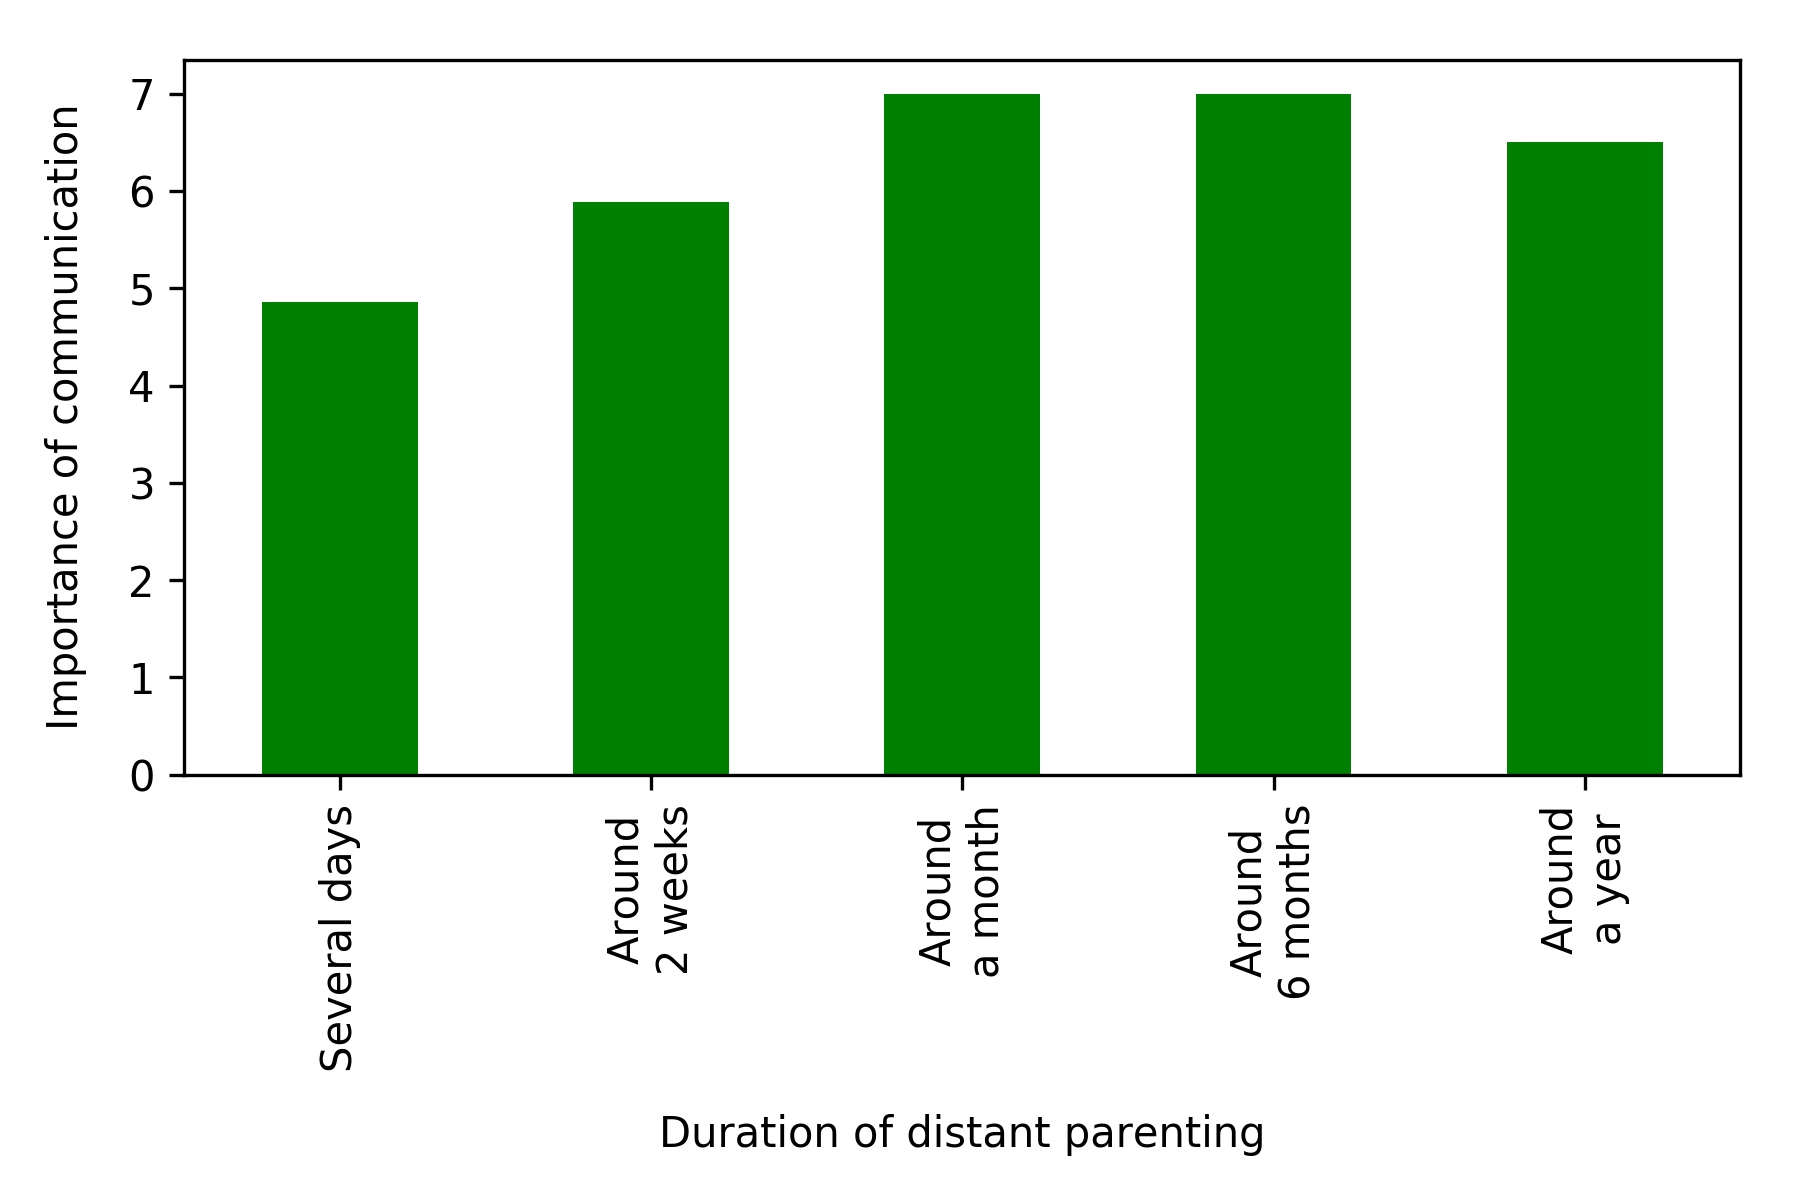
\includegraphics[scale=0.58]{plots/plot_5.png}
    \caption{Importance of communication from the parent point according to duration of distant-parenting experience}
    \label{fig:plot_5}
\end{figure}

\begin{figure}[h!]
    \centering
    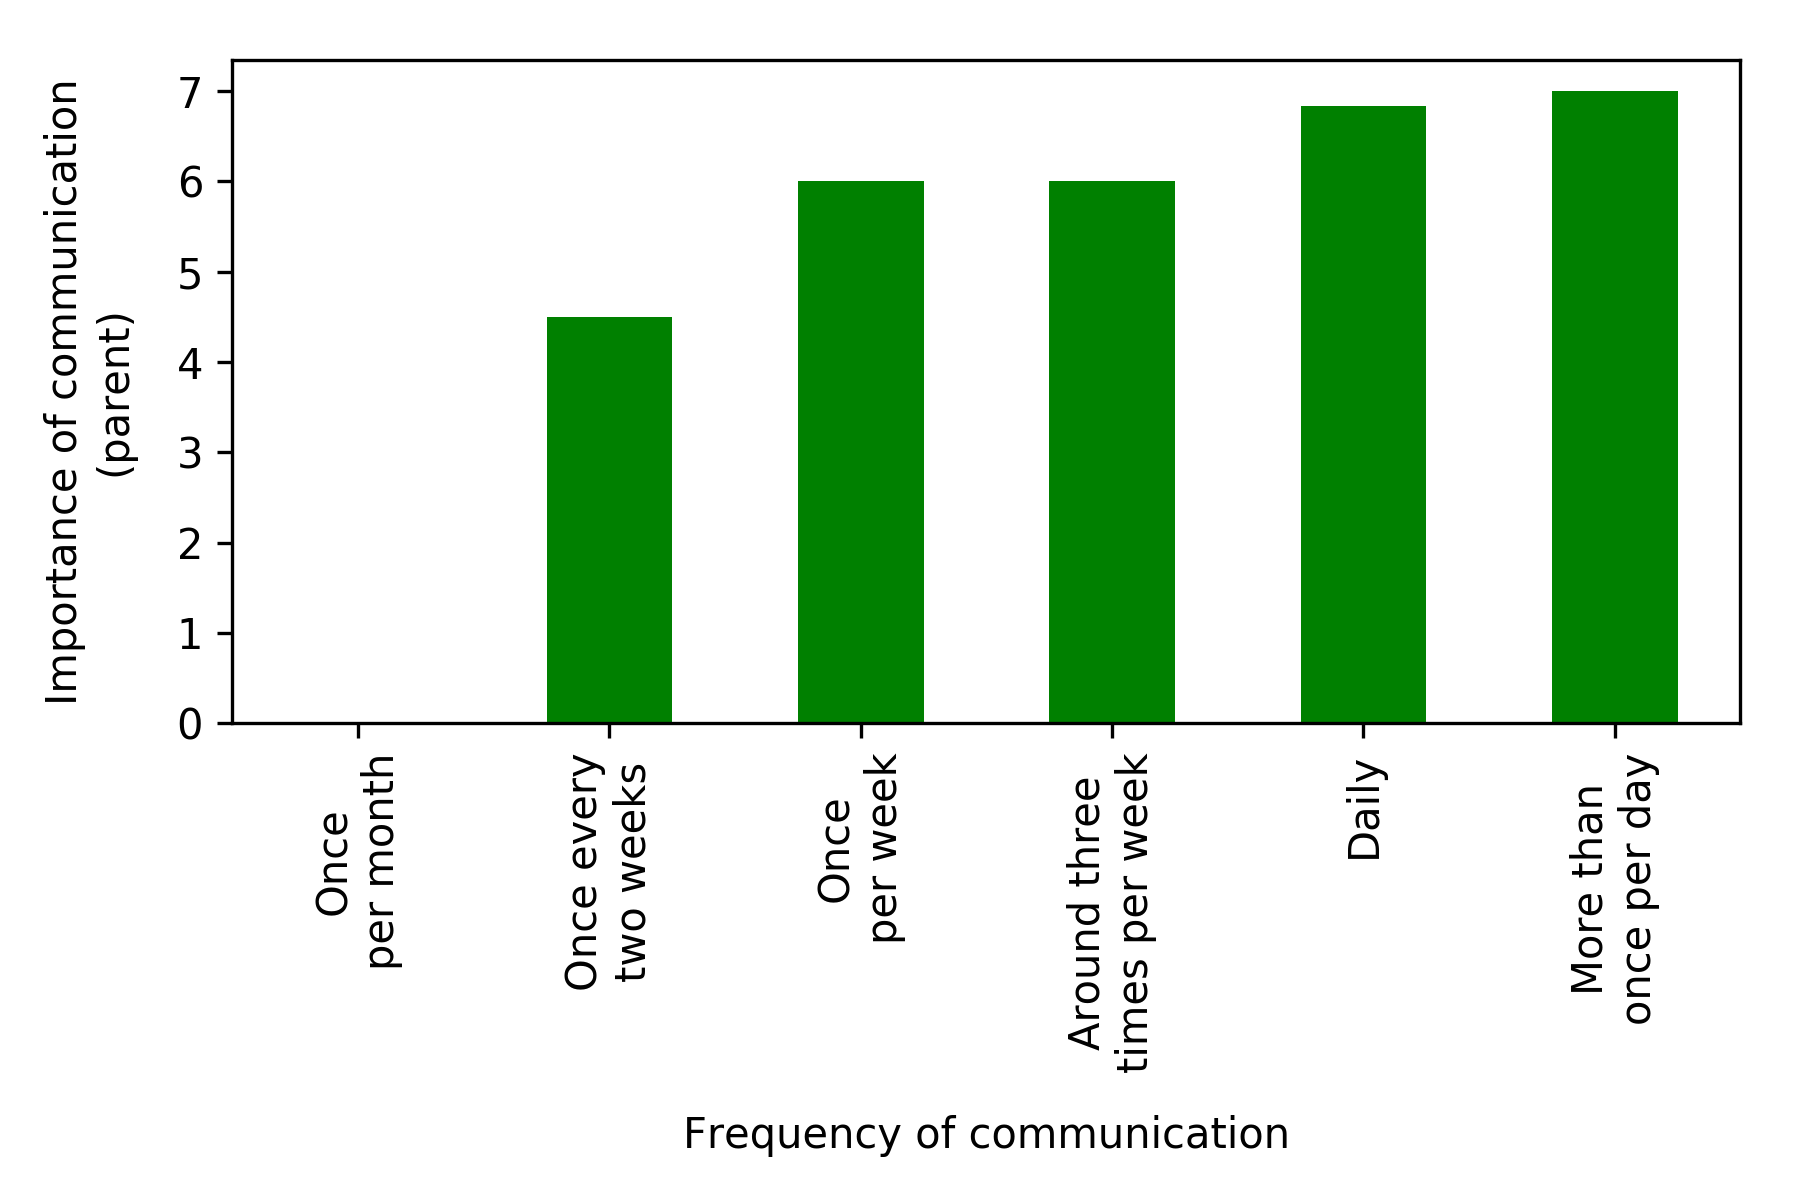
\includegraphics[scale=0.58]{plots/plot_8.png}
    \caption{Importance of communication from the parent point according to frequency of communication during distant-parenting experience}
    \label{fig:plot_8}
\end{figure}


\subsection{Interview protocol}
\label{appendix:interview_protocol}

The following interview protocol has been prepared for the research on “Communication Technologies for Left-Behind Children in Rural China”, in the scope of the “Global perspectives, local realities” SHS course. To continue our research on the Chinese field, by interviewing parents of left behind children, our assumptions could be tested and eventually further analyzed.

\vspace{4pt}
Please, fill in the missing informations as follows before starting the interview session:

Author: Matteo Yann Feo \& Simone Sanso

Session length: 40 minutes 

Participant Name: \hfill \_\_\_\_\_\_\_\_\_\_\_\_\_\_\_\_\_\_\_\_\_\_\_  $\leftarrow$ Fill in

Email: \hfill \_\_\_\_\_\_\_\_\_\_\_\_\_\_\_\_\_\_\_\_\_\_\_\_\_\_\_\_\_\_\_\_ $\leftarrow$ Fill in

Time/Date: \hfill \_\_\_\_\_\_\_\_\_\_\_\_\_\_\_\_\_\_\_\_\_\_\_\_\_\_\_\_ $\leftarrow$ Fill in

Location: \hfill \_\_\_\_\_\_\_\_\_\_\_\_\_\_\_\_\_\_\_\_\_\_\_\_\_\_\_\_\_ $\leftarrow$ Fill in

\vspace{6pt}
\subsubsection{Introduction \& Setup (5 mins)}

The session starts with a short introduction to what this interview is about, the context and the background for which it is being conducted. In the meantime, be sure that everything is setup correctly by double checking the following To-Do list:

\begin{todolist}
    \item Setup the recording tools and check if they work correctly.
    \item Prepare note-taking utilities, such as pen and paper.
    \item Verify the environment, being sure to have a relaxed location for the following 40 mins.
    \item In case a beverage is desired in the meantime, be sure to have it ready and available now.
    \item Be sure that your interviewed person has everything needed.
\end{todolist}

The introduction of the interview could be similar to the following one:

"Good morning and thank you for participating! I am Yann. I am studying at EPFL for a master degree in computer science. My main interest for this interview is to understand whether  a  technology  of  communication embedded in a smart toy could be helpful for parents distant from their children. During the interview, I will be having a conversation with you, asking questions that could help me to achieve my curiosity. In the meantime, my partner, will be assisting me by taking some notes. It is important to always remember that we are not evaluating you or your opinions in any way, there are no possible right and wrong answers that you could give. 
Here is how the session is going to proceed. Firstly, we'll break the ice by asking you a few general questions to know each other. We will record this interview, given your consent. We won't ever share this recording nor use it for anything else but pure support for this interview, so that I can go back and review things later to make sure we got everything right. Your name won't ever be linked to any result, so be relaxed and feel free to share your thoughts with us, without any troubles. Keep in mind that this is completely voluntary, the recording can be stopped whenever you want. Thus, if you don't like this idea, please let me know. 
How does all that sound to you? Do you have any questions at this point?"

\begin{todolist}
    \item Ask the interviewee to sign the written consent for recording purposes.
\end{todolist}

\vspace{2pt}
\subsubsection{Demographics \& Background (5 mins)}

This section will help us to create a background of the interviewee, while allowing him/her to start opening up to our questions. Use this session as a warming-up occasion to break the ice, while catching the first important features. Start to note down details on the interviewee, like gender, age, education level, marital status.

\begin{todolist}
    \item Tell us your name, and a little bit about yourself.
    \item Where do you come from?
    \item What is your occupation? Are you studying or working? In both cases, can you tell us something about it?
    \item Where are you currently living? Do you live with someone, or alone? 
\end{todolist}

\vspace{2pt}
\subsubsection{Main questions (20 mins)}

The following questions can be helpful to interpolate your impressions with the interviewee’s feelings and personal stories. Use them carefully as they might be intimidating for some people. Don’t forget to check for nonverbal behaviors, as they might be critical to have a complete idea of who you are interviewing, especially in this part. Note that the most important questions to be answered are marked with an asterisk (*).

\vspace{2pt}
(*) Pre-interview questions about their children :

\begin{todolist}
    \item How many children do you have?
    \item How old are they?
    \item What gender are they?
    \item Where do you they live?
    \item With who are they staying in your home village? (Lonely, with one of both parents, with grandparents or other relatives)
\end{todolist}

Main interview questions about the interviewed parent :

\begin{todolist}
    \item (*) How often and for how long do you come back home? 
    \item What is the main reason why you live far away from your children?
    \item How do you feel about this situation, not living with your children?
    \item Remember the last time you went back to your home village, how was the contact with your children? Was the meeting with your children as before you left them?
    \item During your childhood, have you ever experienced living far away from one of your parents? If yes, for how long? How did you live the situation? Could you tell us what was the main reason of your parent to out-migrate? How was the contact when meeting again with your parent? Could you communicate together, at that time, while being distant? (Check for non-verbal reactions while interviewee showcase personal experience)
    \item How common is your situation of distant parenting? Do you know any other persons in the same situation as you? How do they live it?
    \item (*) How would you define the importance of living with your children? In your case, is there a trade off between living with your children and having a job position? If yes, imagine that you could live in an ideal world, what would be the best solution? Would you rather work in your home village or be able to bring your children in town?
    \item (*) Do you own electronic devices? If yes, which ones? (Smartphone, computer, more…)
    \item (*) Do your children in your home village own electronic devices? If not, would they have the opportunity to use any? (Neighbourhood, school, etc.)
    \item (*) Do you use electronic devices to contact your children? If yes, how often? In general, are you calling your children when you have time? Or do they also get in touch with you, on their initiative?
    \item (*) From 0 to 7, how would you define the importance of communicating with your children? (0: insignificant, 4: neutral, 7: essential) (Check for non-verbal reactions while interviewee showcase personal experience)
\end{todolist}

\vspace{2pt}
\subsubsection{Interviewee's "show and tell" prototype (8 mins)}

This section is practical and allows us to showcase our project, related to the issue of distant parenting. In the context of CHIC (China Hardware Innovation Camp), a plush toy that encourages social interaction between parents and children, in a distant situation. It is a very resourceful moment, as it could bring additional and authentic feedback on a novel user scenario.

The explanation of the prototype could be similar to the following one:

"We have been working on this prototype. It is a plush toy that encourages social interaction, by having remotely turned on LEDs and sounds from a mobile application. Parents and children can therefore stay longer connected. Letting your children know when you think about them will help you stay 'toygether'\texttrademark."

Showcase the prototype and how it works with the mobile application.

\begin{todolist}
    \item What do you think about the idea?
    \item In your opinion, which are the positive and negative aspects?
    \item If you had the possibility to try this technology, would you be interested?
    \item What would you modify to improve it?
\end{todolist}

\vspace{2pt}
\subsubsection{Closing (2 mins)}

Thank the user at the end for participating to the session. Offer the possibility to ask any kind of question the interviewee might want to address you.  This is his/her time to wear the interviewer's shoes in your regards.

If the interviewee has no additional question, the interview is officially finished. Thank again your interviewee for the time and availability to participate to this session. Underline how useful his/her help has been for the project.
Turn off the recording tools only when you are completely sure that nothing will be added. It is important to not miss anything, so better have some extra recording to cut later.

Take some time to, directly after the end of the interview, write down some impressions you may have about the session. It is important to note down very early impressions about both verbal and physical languages, before they are forgotten. Those are the most authentic resources to get.




\subsection{List of contacts}
\label{appendix:contacts_list}
Below are listed all the contacts that have been reached, to spread as much as possible the survey.

\begin{itemize}
\item AFS programs for adolescents (15-18 years old): \\
Duration: 1 year \\
Kernstrasse 57, CH-8004 Zurich \\
Tel: +41 21 323 19 19 \\
Email: hello@afs.ch \\
https://www.afs.ch/fr/programmes-scolaires/ 

\vspace{4pt}
\item Canada-France exchange (16 years old): \\
Duration : 3 weeks \\
College of Jeanne d'Arc, 15 Rue du Chanoine Brun, 68100 Mulhouse, France \\
Tel: +33 3 89 45 36 31 \\
www.ejda.fr/ 

\vspace{4pt}
\item International exchange programs (14-18 years old): \\
Duration: 1 year \\
Rue Centrale 15, 1003 Lausanne \\
Tel: +41 800 822 811 \\
https://www.efswiss.ch/fr/highschool/ 

\vspace{4pt}
\item National observatory of the Erasmus + impact (1 year or 6 months): \\
Email: observatoire@agence-erasmus.fr \\
http://www.agence-erasmus.fr/page/observatoire/

\vspace{4pt}
\item Journal of international mobility:\\
Email: revue@agence-erasmus.fr \\
https://www.agence-erasmus.fr/page/JIM

\vspace{4pt}
\item Exchange program Brigitte Sauzay (14-17 years old): \\
Duration: 3 months in a host family in Germany and welcome 3 months in the family in France \\
https://www.ofaj.org/contact.html 

\vspace{4pt}
\item Internal exchanges and language stays in Switzerland (14-17 years old): \\
Duration: 1 year \\
College of Delémont, Avenue Station 7, 2800 Delémont \\
Tel: +41 32 421 00 70 \\
Email: info@coldel.org \\
http://www.college-delemont.ch/fr/Aide-aux-eleves/Echanges-et-sejours-linguistiques/Echanges-et-sejours-linguistiques.html \\
Cantonal manager of linguistic exchanges: \\
Patrice KAMBER, Pâquerettes 2, 2822 Courroux \\
- Prof: 032 435 65 92 / Private: 032 422 83 62 

\vspace{4pt}
\item Language Exchange and Mobility - DIP Geneva: \\
Catherine Fernandez Sonino: Head of Exchange \& Mobility DIP of the Cantonal Office for Language Exchange and Mobility \\
Chemin de l'Echo 5a, 1213 Onex \\
Email: catherine.fernandez@etat.ge.ch \\
Tel: +41 22 327 06 43, +41 79 175 56 46 \\
https://edu.ge.ch/site/elem/ 

\vspace{4pt}
\item Service of primary and secondary schools of Lausanne: \\
Place Chauderon 9, 5th floor, PO Box 5032, 1002 Lausanne \\
Tel: +41 21 315 64 11 - Fax: +41 21 315 60 04 \\
Email: seps@lausanne.ch \\
http://www.lausanne.ch/etablissements-scolaires/ 

\vspace{4pt}
\item Summer camp of Neuchatel:\\
Gisèle Nicaty \\
Quartier du Milieu 86, 2127 Les Bayards \\
Tel: +41 79 288 50 41, +41 32 866 17 29\\
Email: giroud.p-a@bluewin.ch\\
http://www.echanges-scolaires.com/index.php/fr/

\vspace{4pt}
\item Summer camp of the Grandes-Roches: \\
1348 le Brassus \\
Tel: +41 21 845 66 90 \\
Email: camps@asime.ch \\
http://www.grandesroches.ch/home 

\vspace{4pt}
\item Association of the Gros-de-Vaud Holiday Camp: \\
Mrs Florence Ethenoz \\
Chemin du Petit Record 60, 1040 Echallens \\
Tel: +41 21 881 10 76 \\
Email: info@colo-gros-de-vaud.ch \\
http://www.colo-gros-de-vaud.ch/clubdesk/www

\vspace{4pt}
\item Summer camp 4Fun: \\
Email: airfred@hotmail.com \\
http://4-fun.ch/ 

\vspace{4pt}
\item Summer camp CPV: \\
Swiss Village Street 14, PO Box 72, 1211 Geneva 8 \\
Tel: +41 22 809 49 79 \\
Email: info@camps.ch \\
http://www.camps.ch/fr/accueil 

\vspace{4pt}
\item Scouts of the Sacred Heart: \\
Jeanne Voruz \& Anne Thiébaud \\
Tel: +41 79 844 92 74 \& +41 79 284 50 38 \\
Email: cg@sacrescout.ch \\
http://www.sacrescout.ch/ 

\vspace{4pt}
\item Village Camps: \\
PO Box 1425, Rue de la Morache 14, 1260 Nyon 1 \\
Tel: +41 22 990 9400 \\
Email: camps@villagecamps.com \\
www.villagecamps.com

\vspace{4pt}
\item Alpadia Language Schools: \\
Grand-Rue 42, PO Box 1206, 1820 Montreux\\
Tel: +41 21 621 88 88\\
Email: info@alpadia.com\\
https://www.alpadia.com/fr/ 

\vspace{4pt}
\item Carol Panchaud Educom sàrl: \\
26 Route of Givrins, CH - 1276 Gingins\\
Tel: +41 22 776 69 15 \\
Email: carolpanchaud@educom.ch \\
http://educom.ch/fr

\vspace{4pt}
\item Caritas-Youth: \\
11, Jean-Violette Street, 1205 Geneva\\
Tel: +41 22 708 04 04\\
Email: info@caritas-jeunesse.ch\\
http://www.caritas-jeunesse.ch/

\vspace{4pt}
\item Holiday Camp St. Gervais: \\
CP 1337, 1211 Geneva 1\\
Tel: +41 78 896 71 84\\
Email: info@colonie-saint-gervais.ch\\
http://www.colonie-saint-gervais.ch/

\vspace{4pt}
\item Summer Camp of Ravoire - Camp Plein Soleil: \\
PO Box 87, CH-1920 Martigny 1\\
Email: info@camp-pleinsoleil.ch

\vspace{4pt}
\item Yverdon-les-Bains youth service and social cohesion: \\
Rue de Neuchâtel 2, 1400 Yverdon-les-Bains\\
Tel: +41 24 423 69 11\\
Email: vacances@yverdon-les-bains.ch\\
http://www.yverdon-les-bains.ch/prestations-deladministration/jeunesse-et-cohesion-sociale/enfanceetfamille/colonies-dete-et-dautomne/

\vspace{4pt}
\item fRilingue GmbH: \\
Stöckackerstrasse 93, 3018 Bern\\
Tel: +41 26 321 34 34 \\
Email: info@frilingue.com

\vspace{4pt}
\item Star Sports: \\
Path of Verger 2, PO Box 101, 1304 Cossonay-Ville\\
Tel: +41 79 356 44 61\\
Email: info@starsports.ch\\
http://www.starsports.ch/

\vspace{4pt}
\item Cap Loisirs Foundation: \\
34, Boulevard de Saint-Georges, 1205 Geneva\\
Tel: +41 22 731 86 00\\
Email: caploisirs@caploisirs.ch\\
http://www.caploisirs.ch/

\vspace{4pt}
\item SCE Holidays \& Events: \\
Rue de Lausanne 58, 1950 Sion\\
Tel: +41 79 693.33.64\\
Email: info@lescamps.ch\\
https://www.lescamps.ch/\\

\end{itemize}



% References of the Report
\thispagestyle{empty}
\vspace{1cm}
\begin{thebibliography}{9}
\addcontentsline{toc}{section}{References}

\bibitem{lab3-report} 
\textit{Lab 3.0 : Camera \& LCD conceptual design}. \\
CS-473 EPFL. Matteo Yann Feo \& Simone Aron Sanso. November 28th, 2017

\bibitem{lcd-controller} 
\textit{ILI9341 - a-Si TFT LCD Single Chip Driver 240RGBx320 Resolution and 262K color}. 
Rev. 1.11. ILI TECHNOLOGY CORP.

\bibitem{lcd-display} 
\textit{LT24 User Manual}. 
Altera. June 2015
 
\bibitem{avalon-interface} 
\textit{Avalon® Interface Specifications}.
MNL-AVABUSREF. Intel. May 2017.
 
\bibitem{fifo} 
\textit{Single- and Dual-Clock FIFO Megafunction}.
Rev. 4.0. Altera. May 2007.

\end{thebibliography}

\end{document}


\documentclass[a4paper,12pt]{article}

%% Layout
\usepackage[utf8]{inputenc}
\usepackage{palatino}
\usepackage[T1]{fontenc}
\usepackage[8pt]{extsizes}

\usepackage{geometry}
\geometry{
    a4paper,
    total={170mm,257mm},
    left=30mm,
    right=30mm,
    top=30mm,
    bottom=30mm,
 } 

%% Useful packages
\usepackage{amsmath}
\usepackage{amssymb}
\usepackage{mathtools}
\usepackage{microtype}

\usepackage[usenames, dvipsnames]{xcolor}
\usepackage{graphicx}
\usepackage{wrapfig}
\usepackage{subfig}
\usepackage{tabularx}
\usepackage{float}
\usepackage{caption}
\usepackage{multirow}
\usepackage{color, colortbl}
\usepackage{enumerate}

\usepackage{hyperref}
\usepackage{url}

\usepackage[english]{babel}
\usepackage{units}

\usepackage{textcomp}
\usepackage{titling}
\usepackage{blindtext}
\usepackage{listings}

\usepackage{braket}
\usepackage{rotating}

%\setlength{\droptitle}{-4em}     % Eliminate the default vertical space
%\addtolength{\droptitle}{-4pt}

\title{
    \centering
	
\includegraphics[width=0.5\textwidth]{images/Logo_EPFL.png}
    \\[1cm]
	\Huge China Hardware Innovation Camp\\[1cm]
    \huge Semester project report\\
    \rule{3.5cm}{0.9pt}\\[0.5cm]
    \huge HUM - 498 \vfill
    \normalsize
}

\author{
    \textbf{Laboratory group:}\\\\
    Chloe Dickson - \texttt{\href{mailto:chloe.dickson@epfl.ch}{simone.sanso@epfl.ch}} \\
    Matteo Yann Feo -    \texttt{\href{mailto:matteo.feo@epfl.ch}{matteo.feo@epfl.ch}} \\
    Simone Aron Sanso - \texttt{\href{mailto:simone.sanso@epfl.ch}{simone.sanso@epfl.ch}} \\\\
}

\date{\vfill \today}

\lstdefinestyle{Python}{
  language=Python,                % choose the language of the code
  numbers=left,                   % where to put the line-numbers
  stepnumber=1,                   % the step between two line-numbers.        
  numbersep=5pt,                  % how far the line-numbers are from the code
  backgroundcolor=\color{white},  % choose the background color. You must add \usepackage{color}
  showspaces=false,               % show spaces adding particular underscores
  showstringspaces=false,         % underline spaces within strings
  showtabs=false,                 % show tabs within strings adding particular underscores
  tabsize=2,                      % sets default tabsize to 2 spaces
  captionpos=b,                   % sets the caption-position to bottom
  breaklines=true,                % sets automatic line breaking
  breakatwhitespace=true,         % sets if automatic breaks should only happen at whitespace
  frame=single, 
  basicstyle=\ttfamily,
  keywordstyle=\color{Green}\bfseries,
  stringstyle=\color{red}\ttfamily,
  commentstyle=\color{OliveGreen}\ttfamily,
  %morecomment=[l][\color{magenta}]{\#}
}


\begin{document}
\maketitle
\thispagestyle{empty}

\newpage
\thispagestyle{empty}
\setcounter{page}{0}

\tableofcontents

\documentclass[a4paper,12pt]{article}

%% Layout
\usepackage[utf8]{inputenc}
\usepackage{palatino}
\usepackage[T1]{fontenc}
\usepackage[8pt]{extsizes}

\usepackage{geometry}
\geometry{
    a4paper,
    total={170mm,257mm},
    left=30mm,
    right=30mm,
    top=30mm,
    bottom=30mm,
 } 

%% Useful packages
\usepackage{amsmath}
\usepackage{amssymb}
\usepackage{mathtools}
\usepackage{microtype}

\usepackage[usenames, dvipsnames]{xcolor}
\usepackage{graphicx}
\usepackage{wrapfig}
\usepackage{subfig}
\usepackage{tabularx}
\usepackage{float}
\usepackage{caption}
\usepackage{multirow}
\usepackage{color, colortbl}
\usepackage{enumerate}

\usepackage{hyperref}
\usepackage{url}

\usepackage[english]{babel}
\usepackage{units}

\usepackage{textcomp}
\usepackage{titling}
\usepackage{blindtext}
\usepackage{listings}

\usepackage{braket}
\usepackage{rotating}

%\setlength{\droptitle}{-4em}     % Eliminate the default vertical space
%\addtolength{\droptitle}{-4pt}

\title{
    \centering
	
\includegraphics[width=0.5\textwidth]{images/Logo_EPFL.png}
    \\[1cm]
	\Huge China Hardware Innovation Camp\\[1cm]
    \huge Semester project report\\
    \rule{3.5cm}{0.9pt}\\[0.5cm]
    \huge HUM - 498 \vfill
    \normalsize
}

\author{
    \textbf{Laboratory group:}\\\\
    Chloe Dickson - \texttt{\href{mailto:chloe.dickson@epfl.ch}{simone.sanso@epfl.ch}} \\
    Matteo Yann Feo -    \texttt{\href{mailto:matteo.feo@epfl.ch}{matteo.feo@epfl.ch}} \\
    Simone Aron Sanso - \texttt{\href{mailto:simone.sanso@epfl.ch}{simone.sanso@epfl.ch}} \\\\
}

\date{\vfill \today}

\lstdefinestyle{Python}{
  language=Python,                % choose the language of the code
  numbers=left,                   % where to put the line-numbers
  stepnumber=1,                   % the step between two line-numbers.        
  numbersep=5pt,                  % how far the line-numbers are from the code
  backgroundcolor=\color{white},  % choose the background color. You must add \usepackage{color}
  showspaces=false,               % show spaces adding particular underscores
  showstringspaces=false,         % underline spaces within strings
  showtabs=false,                 % show tabs within strings adding particular underscores
  tabsize=2,                      % sets default tabsize to 2 spaces
  captionpos=b,                   % sets the caption-position to bottom
  breaklines=true,                % sets automatic line breaking
  breakatwhitespace=true,         % sets if automatic breaks should only happen at whitespace
  frame=single, 
  basicstyle=\ttfamily,
  keywordstyle=\color{Green}\bfseries,
  stringstyle=\color{red}\ttfamily,
  commentstyle=\color{OliveGreen}\ttfamily,
  %morecomment=[l][\color{magenta}]{\#}
}


\begin{document}
\maketitle
\thispagestyle{empty}

\newpage
\thispagestyle{empty}
\setcounter{page}{0}

\tableofcontents

\input{sections/1_introduction/main.tex}

\input{sections/2_structure/main.tex}
    \input{sections/2_structure/subsection_A.tex}
    \input{sections/2_structure/subsection_B.tex}
    \input{sections/2_structure/subsection_C.tex}
    
\input{sections/3_images_tables/main.tex}

\input{sections/4_code/main.tex}

\input{sections/5_conclusion/main.tex}

\input{appendix.tex}

\input{bibliography.tex}

\end{document}


\documentclass[a4paper,12pt]{article}

%% Layout
\usepackage[utf8]{inputenc}
\usepackage{palatino}
\usepackage[T1]{fontenc}
\usepackage[8pt]{extsizes}

\usepackage{geometry}
\geometry{
    a4paper,
    total={170mm,257mm},
    left=30mm,
    right=30mm,
    top=30mm,
    bottom=30mm,
 } 

%% Useful packages
\usepackage{amsmath}
\usepackage{amssymb}
\usepackage{mathtools}
\usepackage{microtype}

\usepackage[usenames, dvipsnames]{xcolor}
\usepackage{graphicx}
\usepackage{wrapfig}
\usepackage{subfig}
\usepackage{tabularx}
\usepackage{float}
\usepackage{caption}
\usepackage{multirow}
\usepackage{color, colortbl}
\usepackage{enumerate}

\usepackage{hyperref}
\usepackage{url}

\usepackage[english]{babel}
\usepackage{units}

\usepackage{textcomp}
\usepackage{titling}
\usepackage{blindtext}
\usepackage{listings}

\usepackage{braket}
\usepackage{rotating}

%\setlength{\droptitle}{-4em}     % Eliminate the default vertical space
%\addtolength{\droptitle}{-4pt}

\title{
    \centering
	
\includegraphics[width=0.5\textwidth]{images/Logo_EPFL.png}
    \\[1cm]
	\Huge China Hardware Innovation Camp\\[1cm]
    \huge Semester project report\\
    \rule{3.5cm}{0.9pt}\\[0.5cm]
    \huge HUM - 498 \vfill
    \normalsize
}

\author{
    \textbf{Laboratory group:}\\\\
    Chloe Dickson - \texttt{\href{mailto:chloe.dickson@epfl.ch}{simone.sanso@epfl.ch}} \\
    Matteo Yann Feo -    \texttt{\href{mailto:matteo.feo@epfl.ch}{matteo.feo@epfl.ch}} \\
    Simone Aron Sanso - \texttt{\href{mailto:simone.sanso@epfl.ch}{simone.sanso@epfl.ch}} \\\\
}

\date{\vfill \today}

\lstdefinestyle{Python}{
  language=Python,                % choose the language of the code
  numbers=left,                   % where to put the line-numbers
  stepnumber=1,                   % the step between two line-numbers.        
  numbersep=5pt,                  % how far the line-numbers are from the code
  backgroundcolor=\color{white},  % choose the background color. You must add \usepackage{color}
  showspaces=false,               % show spaces adding particular underscores
  showstringspaces=false,         % underline spaces within strings
  showtabs=false,                 % show tabs within strings adding particular underscores
  tabsize=2,                      % sets default tabsize to 2 spaces
  captionpos=b,                   % sets the caption-position to bottom
  breaklines=true,                % sets automatic line breaking
  breakatwhitespace=true,         % sets if automatic breaks should only happen at whitespace
  frame=single, 
  basicstyle=\ttfamily,
  keywordstyle=\color{Green}\bfseries,
  stringstyle=\color{red}\ttfamily,
  commentstyle=\color{OliveGreen}\ttfamily,
  %morecomment=[l][\color{magenta}]{\#}
}


\begin{document}
\maketitle
\thispagestyle{empty}

\newpage
\thispagestyle{empty}
\setcounter{page}{0}

\tableofcontents

\input{sections/1_introduction/main.tex}

\input{sections/2_structure/main.tex}
    \input{sections/2_structure/subsection_A.tex}
    \input{sections/2_structure/subsection_B.tex}
    \input{sections/2_structure/subsection_C.tex}
    
\input{sections/3_images_tables/main.tex}

\input{sections/4_code/main.tex}

\input{sections/5_conclusion/main.tex}

\input{appendix.tex}

\input{bibliography.tex}

\end{document}

    %\newpage
\subsection{Subsection A}
\label{subsec:A} 

This is the first subsection. I am saved into a file \textit{subsection\_A.tex} in the same folder as my main file. Pay attention to the format in the label tag in order to reference to the subsection elsewhere. The subsection is called in the main file of the whole document !

\medskip Nunc pulvinar, risus sed gravida pretium, eros tellus vehicula turpis, eget bibendum nisi dolor sed erat. Pellentesque sit amet orci sed ligula dictum cursus. Morbi gravida ligula sapien, non tristique orci semper id. Ut sollicitudin est ut nisi eleifend sollicitudin. Vivamus blandit congue risus id porttitor. Donec sed blandit mauris. Integer est leo, dapibus sed felis et, vulputate sagittis enim. Quisque eget purus vitae metus placerat rhoncus. Nulla eget lacus nec felis tincidunt suscipit ac eget tellus. Ut at augue fermentum, mattis justo sed, consectetur quam. Donec blandit euismod nisi ac auctor.
    %\newpage
\subsection{Subsection B}
\label{subsec:B} 

This is the second subsection. I am also saved into a file \textit{subsection\_B.tex} in the same folder as my main file. Pay attention to the format in the label tag in order to reference to the subsection elsewhere. The subsection is called in the main file of the whole document !

\medskip Nunc pulvinar, risus sed gravida pretium, eros tellus vehicula turpis, eget bibendum nisi dolor sed erat. Pellentesque sit amet orci sed ligula dictum cursus. Morbi gravida ligula sapien, non tristique orci semper id. Ut sollicitudin est ut nisi eleifend sollicitudin. Vivamus blandit congue risus id porttitor. Donec sed blandit mauris. Integer est leo, dapibus sed felis et, vulputate sagittis enim. Quisque eget purus vitae metus placerat rhoncus. Nulla eget lacus nec felis tincidunt suscipit ac eget tellus. Ut at augue fermentum, mattis justo sed, consectetur quam. Donec blandit euismod nisi ac auctor.
    %\newpage
\subsection{Subsection C}
\label{subsec:C} 

Okay, you got it by now ;-)
    
\documentclass[a4paper,12pt]{article}

%% Layout
\usepackage[utf8]{inputenc}
\usepackage{palatino}
\usepackage[T1]{fontenc}
\usepackage[8pt]{extsizes}

\usepackage{geometry}
\geometry{
    a4paper,
    total={170mm,257mm},
    left=30mm,
    right=30mm,
    top=30mm,
    bottom=30mm,
 } 

%% Useful packages
\usepackage{amsmath}
\usepackage{amssymb}
\usepackage{mathtools}
\usepackage{microtype}

\usepackage[usenames, dvipsnames]{xcolor}
\usepackage{graphicx}
\usepackage{wrapfig}
\usepackage{subfig}
\usepackage{tabularx}
\usepackage{float}
\usepackage{caption}
\usepackage{multirow}
\usepackage{color, colortbl}
\usepackage{enumerate}

\usepackage{hyperref}
\usepackage{url}

\usepackage[english]{babel}
\usepackage{units}

\usepackage{textcomp}
\usepackage{titling}
\usepackage{blindtext}
\usepackage{listings}

\usepackage{braket}
\usepackage{rotating}

%\setlength{\droptitle}{-4em}     % Eliminate the default vertical space
%\addtolength{\droptitle}{-4pt}

\title{
    \centering
	
\includegraphics[width=0.5\textwidth]{images/Logo_EPFL.png}
    \\[1cm]
	\Huge China Hardware Innovation Camp\\[1cm]
    \huge Semester project report\\
    \rule{3.5cm}{0.9pt}\\[0.5cm]
    \huge HUM - 498 \vfill
    \normalsize
}

\author{
    \textbf{Laboratory group:}\\\\
    Chloe Dickson - \texttt{\href{mailto:chloe.dickson@epfl.ch}{simone.sanso@epfl.ch}} \\
    Matteo Yann Feo -    \texttt{\href{mailto:matteo.feo@epfl.ch}{matteo.feo@epfl.ch}} \\
    Simone Aron Sanso - \texttt{\href{mailto:simone.sanso@epfl.ch}{simone.sanso@epfl.ch}} \\\\
}

\date{\vfill \today}

\lstdefinestyle{Python}{
  language=Python,                % choose the language of the code
  numbers=left,                   % where to put the line-numbers
  stepnumber=1,                   % the step between two line-numbers.        
  numbersep=5pt,                  % how far the line-numbers are from the code
  backgroundcolor=\color{white},  % choose the background color. You must add \usepackage{color}
  showspaces=false,               % show spaces adding particular underscores
  showstringspaces=false,         % underline spaces within strings
  showtabs=false,                 % show tabs within strings adding particular underscores
  tabsize=2,                      % sets default tabsize to 2 spaces
  captionpos=b,                   % sets the caption-position to bottom
  breaklines=true,                % sets automatic line breaking
  breakatwhitespace=true,         % sets if automatic breaks should only happen at whitespace
  frame=single, 
  basicstyle=\ttfamily,
  keywordstyle=\color{Green}\bfseries,
  stringstyle=\color{red}\ttfamily,
  commentstyle=\color{OliveGreen}\ttfamily,
  %morecomment=[l][\color{magenta}]{\#}
}


\begin{document}
\maketitle
\thispagestyle{empty}

\newpage
\thispagestyle{empty}
\setcounter{page}{0}

\tableofcontents

\input{sections/1_introduction/main.tex}

\input{sections/2_structure/main.tex}
    \input{sections/2_structure/subsection_A.tex}
    \input{sections/2_structure/subsection_B.tex}
    \input{sections/2_structure/subsection_C.tex}
    
\input{sections/3_images_tables/main.tex}

\input{sections/4_code/main.tex}

\input{sections/5_conclusion/main.tex}

\input{appendix.tex}

\input{bibliography.tex}

\end{document}


\documentclass[a4paper,12pt]{article}

%% Layout
\usepackage[utf8]{inputenc}
\usepackage{palatino}
\usepackage[T1]{fontenc}
\usepackage[8pt]{extsizes}

\usepackage{geometry}
\geometry{
    a4paper,
    total={170mm,257mm},
    left=30mm,
    right=30mm,
    top=30mm,
    bottom=30mm,
 } 

%% Useful packages
\usepackage{amsmath}
\usepackage{amssymb}
\usepackage{mathtools}
\usepackage{microtype}

\usepackage[usenames, dvipsnames]{xcolor}
\usepackage{graphicx}
\usepackage{wrapfig}
\usepackage{subfig}
\usepackage{tabularx}
\usepackage{float}
\usepackage{caption}
\usepackage{multirow}
\usepackage{color, colortbl}
\usepackage{enumerate}

\usepackage{hyperref}
\usepackage{url}

\usepackage[english]{babel}
\usepackage{units}

\usepackage{textcomp}
\usepackage{titling}
\usepackage{blindtext}
\usepackage{listings}

\usepackage{braket}
\usepackage{rotating}

%\setlength{\droptitle}{-4em}     % Eliminate the default vertical space
%\addtolength{\droptitle}{-4pt}

\title{
    \centering
	
\includegraphics[width=0.5\textwidth]{images/Logo_EPFL.png}
    \\[1cm]
	\Huge China Hardware Innovation Camp\\[1cm]
    \huge Semester project report\\
    \rule{3.5cm}{0.9pt}\\[0.5cm]
    \huge HUM - 498 \vfill
    \normalsize
}

\author{
    \textbf{Laboratory group:}\\\\
    Chloe Dickson - \texttt{\href{mailto:chloe.dickson@epfl.ch}{simone.sanso@epfl.ch}} \\
    Matteo Yann Feo -    \texttt{\href{mailto:matteo.feo@epfl.ch}{matteo.feo@epfl.ch}} \\
    Simone Aron Sanso - \texttt{\href{mailto:simone.sanso@epfl.ch}{simone.sanso@epfl.ch}} \\\\
}

\date{\vfill \today}

\lstdefinestyle{Python}{
  language=Python,                % choose the language of the code
  numbers=left,                   % where to put the line-numbers
  stepnumber=1,                   % the step between two line-numbers.        
  numbersep=5pt,                  % how far the line-numbers are from the code
  backgroundcolor=\color{white},  % choose the background color. You must add \usepackage{color}
  showspaces=false,               % show spaces adding particular underscores
  showstringspaces=false,         % underline spaces within strings
  showtabs=false,                 % show tabs within strings adding particular underscores
  tabsize=2,                      % sets default tabsize to 2 spaces
  captionpos=b,                   % sets the caption-position to bottom
  breaklines=true,                % sets automatic line breaking
  breakatwhitespace=true,         % sets if automatic breaks should only happen at whitespace
  frame=single, 
  basicstyle=\ttfamily,
  keywordstyle=\color{Green}\bfseries,
  stringstyle=\color{red}\ttfamily,
  commentstyle=\color{OliveGreen}\ttfamily,
  %morecomment=[l][\color{magenta}]{\#}
}


\begin{document}
\maketitle
\thispagestyle{empty}

\newpage
\thispagestyle{empty}
\setcounter{page}{0}

\tableofcontents

\input{sections/1_introduction/main.tex}

\input{sections/2_structure/main.tex}
    \input{sections/2_structure/subsection_A.tex}
    \input{sections/2_structure/subsection_B.tex}
    \input{sections/2_structure/subsection_C.tex}
    
\input{sections/3_images_tables/main.tex}

\input{sections/4_code/main.tex}

\input{sections/5_conclusion/main.tex}

\input{appendix.tex}

\input{bibliography.tex}

\end{document}


\documentclass[a4paper,12pt]{article}

%% Layout
\usepackage[utf8]{inputenc}
\usepackage{palatino}
\usepackage[T1]{fontenc}
\usepackage[8pt]{extsizes}

\usepackage{geometry}
\geometry{
    a4paper,
    total={170mm,257mm},
    left=30mm,
    right=30mm,
    top=30mm,
    bottom=30mm,
 } 

%% Useful packages
\usepackage{amsmath}
\usepackage{amssymb}
\usepackage{mathtools}
\usepackage{microtype}

\usepackage[usenames, dvipsnames]{xcolor}
\usepackage{graphicx}
\usepackage{wrapfig}
\usepackage{subfig}
\usepackage{tabularx}
\usepackage{float}
\usepackage{caption}
\usepackage{multirow}
\usepackage{color, colortbl}
\usepackage{enumerate}

\usepackage{hyperref}
\usepackage{url}

\usepackage[english]{babel}
\usepackage{units}

\usepackage{textcomp}
\usepackage{titling}
\usepackage{blindtext}
\usepackage{listings}

\usepackage{braket}
\usepackage{rotating}

%\setlength{\droptitle}{-4em}     % Eliminate the default vertical space
%\addtolength{\droptitle}{-4pt}

\title{
    \centering
	
\includegraphics[width=0.5\textwidth]{images/Logo_EPFL.png}
    \\[1cm]
	\Huge China Hardware Innovation Camp\\[1cm]
    \huge Semester project report\\
    \rule{3.5cm}{0.9pt}\\[0.5cm]
    \huge HUM - 498 \vfill
    \normalsize
}

\author{
    \textbf{Laboratory group:}\\\\
    Chloe Dickson - \texttt{\href{mailto:chloe.dickson@epfl.ch}{simone.sanso@epfl.ch}} \\
    Matteo Yann Feo -    \texttt{\href{mailto:matteo.feo@epfl.ch}{matteo.feo@epfl.ch}} \\
    Simone Aron Sanso - \texttt{\href{mailto:simone.sanso@epfl.ch}{simone.sanso@epfl.ch}} \\\\
}

\date{\vfill \today}

\lstdefinestyle{Python}{
  language=Python,                % choose the language of the code
  numbers=left,                   % where to put the line-numbers
  stepnumber=1,                   % the step between two line-numbers.        
  numbersep=5pt,                  % how far the line-numbers are from the code
  backgroundcolor=\color{white},  % choose the background color. You must add \usepackage{color}
  showspaces=false,               % show spaces adding particular underscores
  showstringspaces=false,         % underline spaces within strings
  showtabs=false,                 % show tabs within strings adding particular underscores
  tabsize=2,                      % sets default tabsize to 2 spaces
  captionpos=b,                   % sets the caption-position to bottom
  breaklines=true,                % sets automatic line breaking
  breakatwhitespace=true,         % sets if automatic breaks should only happen at whitespace
  frame=single, 
  basicstyle=\ttfamily,
  keywordstyle=\color{Green}\bfseries,
  stringstyle=\color{red}\ttfamily,
  commentstyle=\color{OliveGreen}\ttfamily,
  %morecomment=[l][\color{magenta}]{\#}
}


\begin{document}
\maketitle
\thispagestyle{empty}

\newpage
\thispagestyle{empty}
\setcounter{page}{0}

\tableofcontents

\input{sections/1_introduction/main.tex}

\input{sections/2_structure/main.tex}
    \input{sections/2_structure/subsection_A.tex}
    \input{sections/2_structure/subsection_B.tex}
    \input{sections/2_structure/subsection_C.tex}
    
\input{sections/3_images_tables/main.tex}

\input{sections/4_code/main.tex}

\input{sections/5_conclusion/main.tex}

\input{appendix.tex}

\input{bibliography.tex}

\end{document}


% Appendix of the Report
\appendix

In the following appendix are presented the questions of the survey (... a list of figures and tables) to the reader.

\subsection{Questions of the survey}
\label{appendix:survey_questions}
In this section is shown how the participants were questioned towards the survey. Only the questions in English will be shown here, skipping the French translations.

\medskip \textit{Form about communication technologies :} \\
Realizing a research project about social sciences within EPFL University (Lausanne), we would like to understand the importance of communication between parents and children, when they are at a distance during a continuous period of time.

\vspace{4pt}
1. In what language would like to answer this form?

2. To contextualize, we seek either :

- parents of a child having spent a period of time away from the household,

- children, teenagers and young adults having spent a period of time away from their family.

After having read the description above, do you qualify yourself as a parent or a child?

\vspace{4pt}
\noindent - If "parent" was selected question 2: 

3.a. Are you the mother or the father?

4.a. Have you already been separated from your child for at least 3 days? (Exchange semester abroad, holidays, summer camp, boy-scout, etc.)

5.a. If there were more than one experience of distance parenting, please consider the earliest one of them through the rest of the form (when you were the youngest). What is the reason why your child was distant from you? 

6.a. For how long have you been distant from your child?

7.a. How old was your child at that time?

8.a. What is your child's gender?

9.a. How often did you use a communication technology with your distant child? (Text messages, phone calls, video chat, etc.)

10.a. What kind of information did you seek from communicating with your distant child?

11.a. How would you define the importance of being able to communicate with your distant child?

\vspace{4pt}
\noindent - If "child" was selected question 2: 

3.b. Have you already been separated from your family for at least 3 days? (Exchange semester abroad, holidays, summer camp, boy-scout, etc.)

3.b. If there were more than one experience of separation from your family, please consider the earliest one of them through the rest of the form (when you were the youngest). What is the reason why you were distant from your family? 

4.b. For how long have you been away?

5.b. How old were you at that time?

6.b. What is your gender?

7.b. How often did you use a communication technology with your family? (Text messages, phone calls, video chat, etc.)

8.b. What kind of information did you seek from communicating with your family?

9.b. How would you define the importance of being able to communicate with your family?


\subsection{Additional plots of the results}
\label{appendix:additional-plots}

The following plots have been computed for the analysis of the data collected via the survey on distant-parenting. This appendix contains a set of plots that didn't need particular attention during the discussion, but can still be source of investigation.

\begin{figure}[h!]
    \centering
    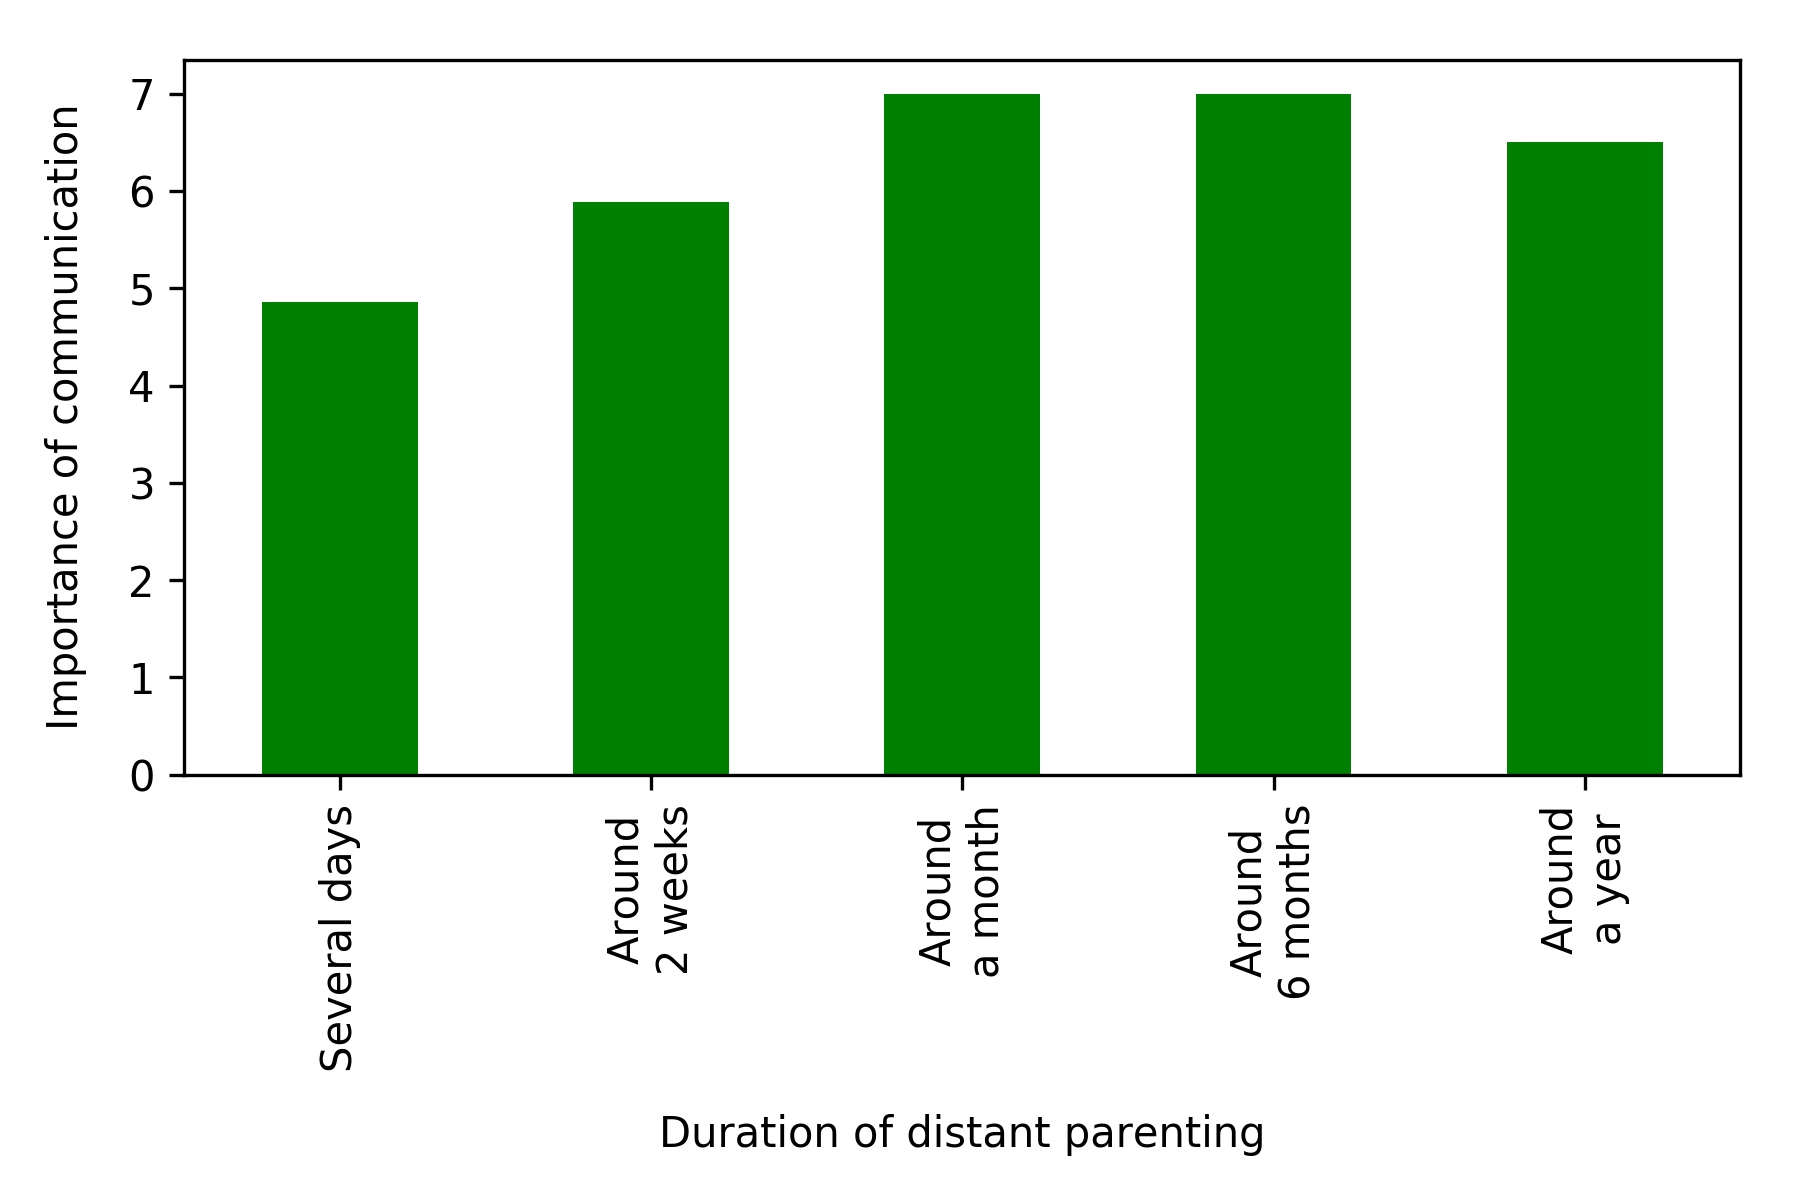
\includegraphics[scale=0.58]{plots/plot_5.png}
    \caption{Importance of communication from the parent point according to duration of distant-parenting experience}
    \label{fig:plot_5}
\end{figure}

\begin{figure}[h!]
    \centering
    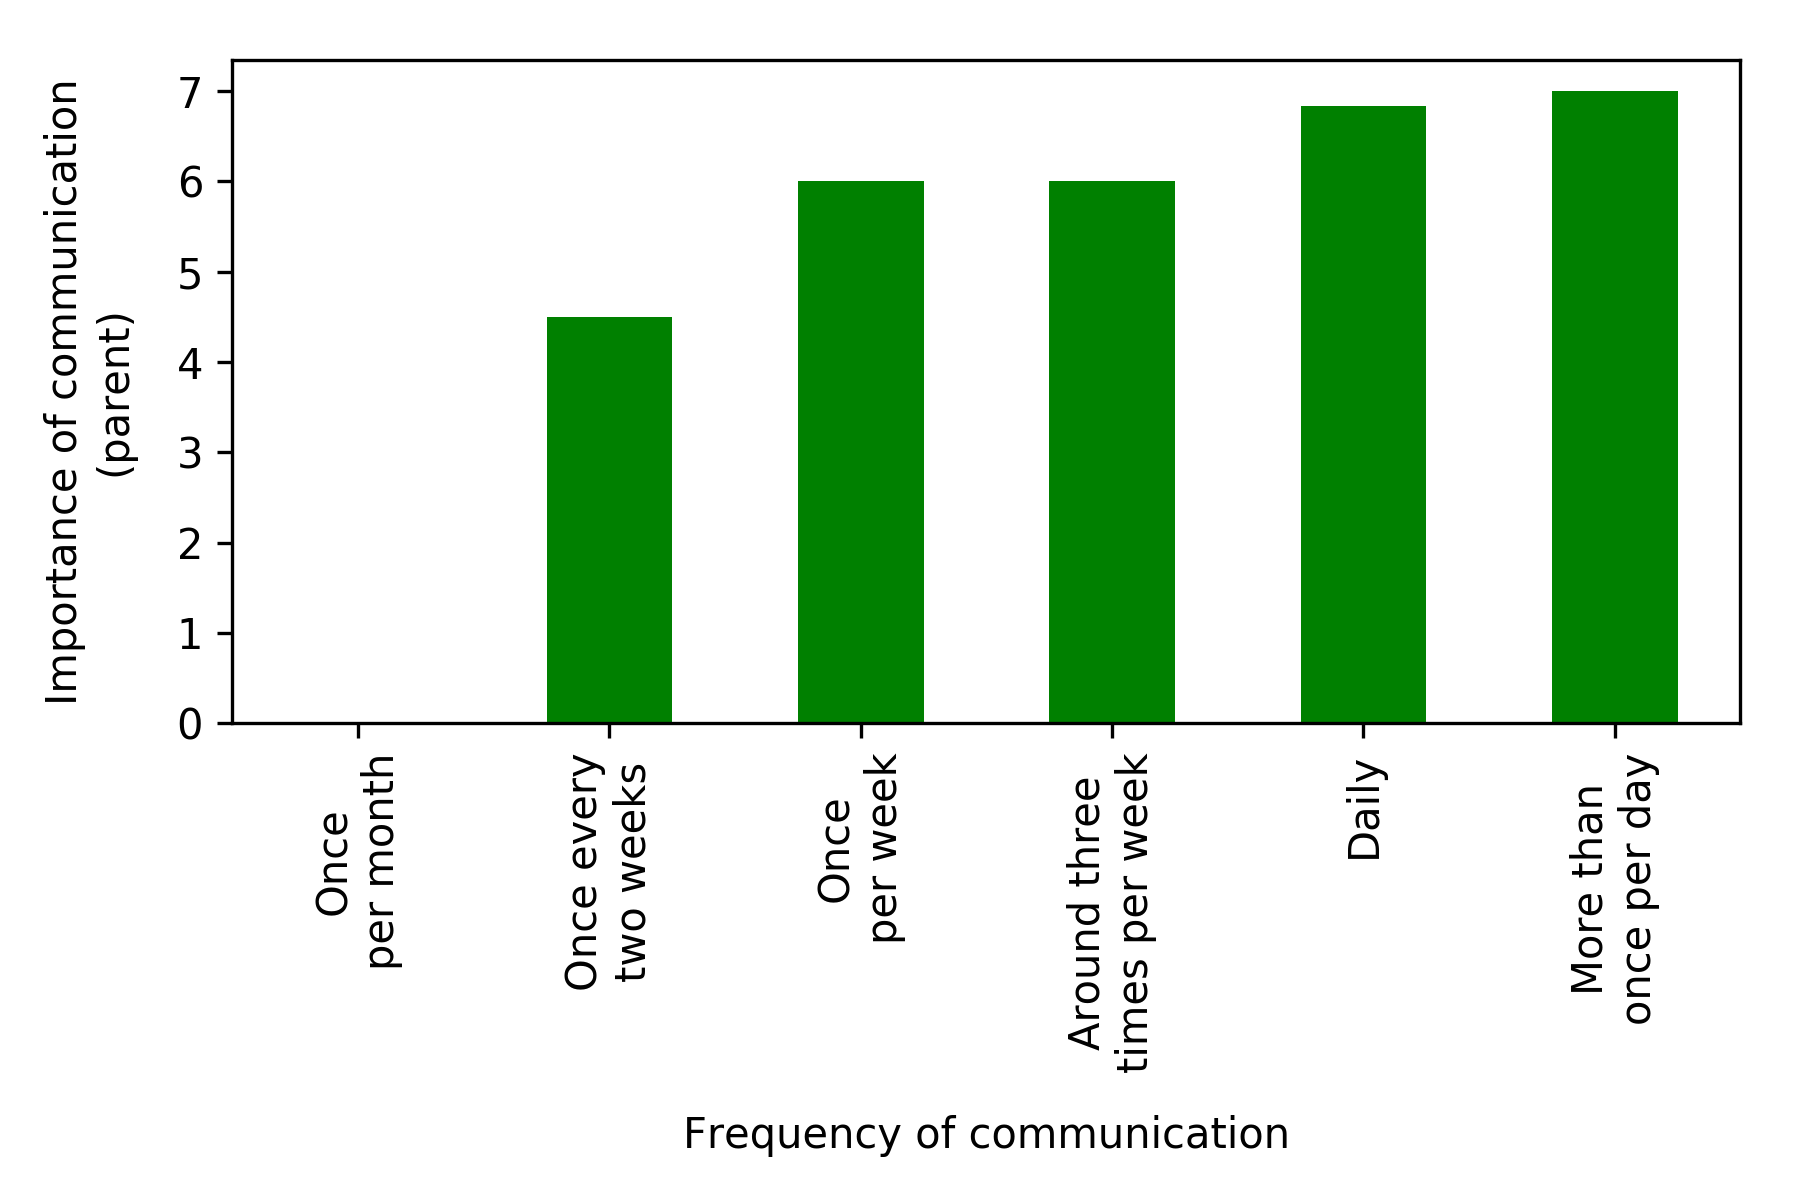
\includegraphics[scale=0.58]{plots/plot_8.png}
    \caption{Importance of communication from the parent point according to frequency of communication during distant-parenting experience}
    \label{fig:plot_8}
\end{figure}


\subsection{Interview protocol}
\label{appendix:interview_protocol}

The following interview protocol has been prepared for the research on “Communication Technologies for Left-Behind Children in Rural China”, in the scope of the “Global perspectives, local realities” SHS course. To continue our research on the Chinese field, by interviewing parents of left behind children, our assumptions could be tested and eventually further analyzed.

\vspace{4pt}
Please, fill in the missing informations as follows before starting the interview session:

Author: Matteo Yann Feo \& Simone Sanso

Session length: 40 minutes 

Participant Name: \hfill \_\_\_\_\_\_\_\_\_\_\_\_\_\_\_\_\_\_\_\_\_\_\_  $\leftarrow$ Fill in

Email: \hfill \_\_\_\_\_\_\_\_\_\_\_\_\_\_\_\_\_\_\_\_\_\_\_\_\_\_\_\_\_\_\_\_ $\leftarrow$ Fill in

Time/Date: \hfill \_\_\_\_\_\_\_\_\_\_\_\_\_\_\_\_\_\_\_\_\_\_\_\_\_\_\_\_ $\leftarrow$ Fill in

Location: \hfill \_\_\_\_\_\_\_\_\_\_\_\_\_\_\_\_\_\_\_\_\_\_\_\_\_\_\_\_\_ $\leftarrow$ Fill in

\vspace{6pt}
\subsubsection{Introduction \& Setup (5 mins)}

The session starts with a short introduction to what this interview is about, the context and the background for which it is being conducted. In the meantime, be sure that everything is setup correctly by double checking the following To-Do list:

\begin{todolist}
    \item Setup the recording tools and check if they work correctly.
    \item Prepare note-taking utilities, such as pen and paper.
    \item Verify the environment, being sure to have a relaxed location for the following 40 mins.
    \item In case a beverage is desired in the meantime, be sure to have it ready and available now.
    \item Be sure that your interviewed person has everything needed.
\end{todolist}

The introduction of the interview could be similar to the following one:

"Good morning and thank you for participating! I am Yann. I am studying at EPFL for a master degree in computer science. My main interest for this interview is to understand whether  a  technology  of  communication embedded in a smart toy could be helpful for parents distant from their children. During the interview, I will be having a conversation with you, asking questions that could help me to achieve my curiosity. In the meantime, my partner, will be assisting me by taking some notes. It is important to always remember that we are not evaluating you or your opinions in any way, there are no possible right and wrong answers that you could give. 
Here is how the session is going to proceed. Firstly, we'll break the ice by asking you a few general questions to know each other. We will record this interview, given your consent. We won't ever share this recording nor use it for anything else but pure support for this interview, so that I can go back and review things later to make sure we got everything right. Your name won't ever be linked to any result, so be relaxed and feel free to share your thoughts with us, without any troubles. Keep in mind that this is completely voluntary, the recording can be stopped whenever you want. Thus, if you don't like this idea, please let me know. 
How does all that sound to you? Do you have any questions at this point?"

\begin{todolist}
    \item Ask the interviewee to sign the written consent for recording purposes.
\end{todolist}

\vspace{2pt}
\subsubsection{Demographics \& Background (5 mins)}

This section will help us to create a background of the interviewee, while allowing him/her to start opening up to our questions. Use this session as a warming-up occasion to break the ice, while catching the first important features. Start to note down details on the interviewee, like gender, age, education level, marital status.

\begin{todolist}
    \item Tell us your name, and a little bit about yourself.
    \item Where do you come from?
    \item What is your occupation? Are you studying or working? In both cases, can you tell us something about it?
    \item Where are you currently living? Do you live with someone, or alone? 
\end{todolist}

\vspace{2pt}
\subsubsection{Main questions (20 mins)}

The following questions can be helpful to interpolate your impressions with the interviewee’s feelings and personal stories. Use them carefully as they might be intimidating for some people. Don’t forget to check for nonverbal behaviors, as they might be critical to have a complete idea of who you are interviewing, especially in this part. Note that the most important questions to be answered are marked with an asterisk (*).

\vspace{2pt}
(*) Pre-interview questions about their children :

\begin{todolist}
    \item How many children do you have?
    \item How old are they?
    \item What gender are they?
    \item Where do you they live?
    \item With who are they staying in your home village? (Lonely, with one of both parents, with grandparents or other relatives)
\end{todolist}

Main interview questions about the interviewed parent :

\begin{todolist}
    \item (*) How often and for how long do you come back home? 
    \item What is the main reason why you live far away from your children?
    \item How do you feel about this situation, not living with your children?
    \item Remember the last time you went back to your home village, how was the contact with your children? Was the meeting with your children as before you left them?
    \item During your childhood, have you ever experienced living far away from one of your parents? If yes, for how long? How did you live the situation? Could you tell us what was the main reason of your parent to out-migrate? How was the contact when meeting again with your parent? Could you communicate together, at that time, while being distant? (Check for non-verbal reactions while interviewee showcase personal experience)
    \item How common is your situation of distant parenting? Do you know any other persons in the same situation as you? How do they live it?
    \item (*) How would you define the importance of living with your children? In your case, is there a trade off between living with your children and having a job position? If yes, imagine that you could live in an ideal world, what would be the best solution? Would you rather work in your home village or be able to bring your children in town?
    \item (*) Do you own electronic devices? If yes, which ones? (Smartphone, computer, more…)
    \item (*) Do your children in your home village own electronic devices? If not, would they have the opportunity to use any? (Neighbourhood, school, etc.)
    \item (*) Do you use electronic devices to contact your children? If yes, how often? In general, are you calling your children when you have time? Or do they also get in touch with you, on their initiative?
    \item (*) From 0 to 7, how would you define the importance of communicating with your children? (0: insignificant, 4: neutral, 7: essential) (Check for non-verbal reactions while interviewee showcase personal experience)
\end{todolist}

\vspace{2pt}
\subsubsection{Interviewee's "show and tell" prototype (8 mins)}

This section is practical and allows us to showcase our project, related to the issue of distant parenting. In the context of CHIC (China Hardware Innovation Camp), a plush toy that encourages social interaction between parents and children, in a distant situation. It is a very resourceful moment, as it could bring additional and authentic feedback on a novel user scenario.

The explanation of the prototype could be similar to the following one:

"We have been working on this prototype. It is a plush toy that encourages social interaction, by having remotely turned on LEDs and sounds from a mobile application. Parents and children can therefore stay longer connected. Letting your children know when you think about them will help you stay 'toygether'\texttrademark."

Showcase the prototype and how it works with the mobile application.

\begin{todolist}
    \item What do you think about the idea?
    \item In your opinion, which are the positive and negative aspects?
    \item If you had the possibility to try this technology, would you be interested?
    \item What would you modify to improve it?
\end{todolist}

\vspace{2pt}
\subsubsection{Closing (2 mins)}

Thank the user at the end for participating to the session. Offer the possibility to ask any kind of question the interviewee might want to address you.  This is his/her time to wear the interviewer's shoes in your regards.

If the interviewee has no additional question, the interview is officially finished. Thank again your interviewee for the time and availability to participate to this session. Underline how useful his/her help has been for the project.
Turn off the recording tools only when you are completely sure that nothing will be added. It is important to not miss anything, so better have some extra recording to cut later.

Take some time to, directly after the end of the interview, write down some impressions you may have about the session. It is important to note down very early impressions about both verbal and physical languages, before they are forgotten. Those are the most authentic resources to get.




\subsection{List of contacts}
\label{appendix:contacts_list}
Below are listed all the contacts that have been reached, to spread as much as possible the survey.

\begin{itemize}
\item AFS programs for adolescents (15-18 years old): \\
Duration: 1 year \\
Kernstrasse 57, CH-8004 Zurich \\
Tel: +41 21 323 19 19 \\
Email: hello@afs.ch \\
https://www.afs.ch/fr/programmes-scolaires/ 

\vspace{4pt}
\item Canada-France exchange (16 years old): \\
Duration : 3 weeks \\
College of Jeanne d'Arc, 15 Rue du Chanoine Brun, 68100 Mulhouse, France \\
Tel: +33 3 89 45 36 31 \\
www.ejda.fr/ 

\vspace{4pt}
\item International exchange programs (14-18 years old): \\
Duration: 1 year \\
Rue Centrale 15, 1003 Lausanne \\
Tel: +41 800 822 811 \\
https://www.efswiss.ch/fr/highschool/ 

\vspace{4pt}
\item National observatory of the Erasmus + impact (1 year or 6 months): \\
Email: observatoire@agence-erasmus.fr \\
http://www.agence-erasmus.fr/page/observatoire/

\vspace{4pt}
\item Journal of international mobility:\\
Email: revue@agence-erasmus.fr \\
https://www.agence-erasmus.fr/page/JIM

\vspace{4pt}
\item Exchange program Brigitte Sauzay (14-17 years old): \\
Duration: 3 months in a host family in Germany and welcome 3 months in the family in France \\
https://www.ofaj.org/contact.html 

\vspace{4pt}
\item Internal exchanges and language stays in Switzerland (14-17 years old): \\
Duration: 1 year \\
College of Delémont, Avenue Station 7, 2800 Delémont \\
Tel: +41 32 421 00 70 \\
Email: info@coldel.org \\
http://www.college-delemont.ch/fr/Aide-aux-eleves/Echanges-et-sejours-linguistiques/Echanges-et-sejours-linguistiques.html \\
Cantonal manager of linguistic exchanges: \\
Patrice KAMBER, Pâquerettes 2, 2822 Courroux \\
- Prof: 032 435 65 92 / Private: 032 422 83 62 

\vspace{4pt}
\item Language Exchange and Mobility - DIP Geneva: \\
Catherine Fernandez Sonino: Head of Exchange \& Mobility DIP of the Cantonal Office for Language Exchange and Mobility \\
Chemin de l'Echo 5a, 1213 Onex \\
Email: catherine.fernandez@etat.ge.ch \\
Tel: +41 22 327 06 43, +41 79 175 56 46 \\
https://edu.ge.ch/site/elem/ 

\vspace{4pt}
\item Service of primary and secondary schools of Lausanne: \\
Place Chauderon 9, 5th floor, PO Box 5032, 1002 Lausanne \\
Tel: +41 21 315 64 11 - Fax: +41 21 315 60 04 \\
Email: seps@lausanne.ch \\
http://www.lausanne.ch/etablissements-scolaires/ 

\vspace{4pt}
\item Summer camp of Neuchatel:\\
Gisèle Nicaty \\
Quartier du Milieu 86, 2127 Les Bayards \\
Tel: +41 79 288 50 41, +41 32 866 17 29\\
Email: giroud.p-a@bluewin.ch\\
http://www.echanges-scolaires.com/index.php/fr/

\vspace{4pt}
\item Summer camp of the Grandes-Roches: \\
1348 le Brassus \\
Tel: +41 21 845 66 90 \\
Email: camps@asime.ch \\
http://www.grandesroches.ch/home 

\vspace{4pt}
\item Association of the Gros-de-Vaud Holiday Camp: \\
Mrs Florence Ethenoz \\
Chemin du Petit Record 60, 1040 Echallens \\
Tel: +41 21 881 10 76 \\
Email: info@colo-gros-de-vaud.ch \\
http://www.colo-gros-de-vaud.ch/clubdesk/www

\vspace{4pt}
\item Summer camp 4Fun: \\
Email: airfred@hotmail.com \\
http://4-fun.ch/ 

\vspace{4pt}
\item Summer camp CPV: \\
Swiss Village Street 14, PO Box 72, 1211 Geneva 8 \\
Tel: +41 22 809 49 79 \\
Email: info@camps.ch \\
http://www.camps.ch/fr/accueil 

\vspace{4pt}
\item Scouts of the Sacred Heart: \\
Jeanne Voruz \& Anne Thiébaud \\
Tel: +41 79 844 92 74 \& +41 79 284 50 38 \\
Email: cg@sacrescout.ch \\
http://www.sacrescout.ch/ 

\vspace{4pt}
\item Village Camps: \\
PO Box 1425, Rue de la Morache 14, 1260 Nyon 1 \\
Tel: +41 22 990 9400 \\
Email: camps@villagecamps.com \\
www.villagecamps.com

\vspace{4pt}
\item Alpadia Language Schools: \\
Grand-Rue 42, PO Box 1206, 1820 Montreux\\
Tel: +41 21 621 88 88\\
Email: info@alpadia.com\\
https://www.alpadia.com/fr/ 

\vspace{4pt}
\item Carol Panchaud Educom sàrl: \\
26 Route of Givrins, CH - 1276 Gingins\\
Tel: +41 22 776 69 15 \\
Email: carolpanchaud@educom.ch \\
http://educom.ch/fr

\vspace{4pt}
\item Caritas-Youth: \\
11, Jean-Violette Street, 1205 Geneva\\
Tel: +41 22 708 04 04\\
Email: info@caritas-jeunesse.ch\\
http://www.caritas-jeunesse.ch/

\vspace{4pt}
\item Holiday Camp St. Gervais: \\
CP 1337, 1211 Geneva 1\\
Tel: +41 78 896 71 84\\
Email: info@colonie-saint-gervais.ch\\
http://www.colonie-saint-gervais.ch/

\vspace{4pt}
\item Summer Camp of Ravoire - Camp Plein Soleil: \\
PO Box 87, CH-1920 Martigny 1\\
Email: info@camp-pleinsoleil.ch

\vspace{4pt}
\item Yverdon-les-Bains youth service and social cohesion: \\
Rue de Neuchâtel 2, 1400 Yverdon-les-Bains\\
Tel: +41 24 423 69 11\\
Email: vacances@yverdon-les-bains.ch\\
http://www.yverdon-les-bains.ch/prestations-deladministration/jeunesse-et-cohesion-sociale/enfanceetfamille/colonies-dete-et-dautomne/

\vspace{4pt}
\item fRilingue GmbH: \\
Stöckackerstrasse 93, 3018 Bern\\
Tel: +41 26 321 34 34 \\
Email: info@frilingue.com

\vspace{4pt}
\item Star Sports: \\
Path of Verger 2, PO Box 101, 1304 Cossonay-Ville\\
Tel: +41 79 356 44 61\\
Email: info@starsports.ch\\
http://www.starsports.ch/

\vspace{4pt}
\item Cap Loisirs Foundation: \\
34, Boulevard de Saint-Georges, 1205 Geneva\\
Tel: +41 22 731 86 00\\
Email: caploisirs@caploisirs.ch\\
http://www.caploisirs.ch/

\vspace{4pt}
\item SCE Holidays \& Events: \\
Rue de Lausanne 58, 1950 Sion\\
Tel: +41 79 693.33.64\\
Email: info@lescamps.ch\\
https://www.lescamps.ch/\\

\end{itemize}



% References of the Report
\thispagestyle{empty}
\vspace{1cm}
\begin{thebibliography}{9}
\addcontentsline{toc}{section}{References}

\bibitem{lab3-report} 
\textit{Lab 3.0 : Camera \& LCD conceptual design}. \\
CS-473 EPFL. Matteo Yann Feo \& Simone Aron Sanso. November 28th, 2017

\bibitem{lcd-controller} 
\textit{ILI9341 - a-Si TFT LCD Single Chip Driver 240RGBx320 Resolution and 262K color}. 
Rev. 1.11. ILI TECHNOLOGY CORP.

\bibitem{lcd-display} 
\textit{LT24 User Manual}. 
Altera. June 2015
 
\bibitem{avalon-interface} 
\textit{Avalon® Interface Specifications}.
MNL-AVABUSREF. Intel. May 2017.
 
\bibitem{fifo} 
\textit{Single- and Dual-Clock FIFO Megafunction}.
Rev. 4.0. Altera. May 2007.

\end{thebibliography}

\end{document}

    %\newpage
\subsection{Subsection A}
\label{subsec:A} 

This is the first subsection. I am saved into a file \textit{subsection\_A.tex} in the same folder as my main file. Pay attention to the format in the label tag in order to reference to the subsection elsewhere. The subsection is called in the main file of the whole document !

\medskip Nunc pulvinar, risus sed gravida pretium, eros tellus vehicula turpis, eget bibendum nisi dolor sed erat. Pellentesque sit amet orci sed ligula dictum cursus. Morbi gravida ligula sapien, non tristique orci semper id. Ut sollicitudin est ut nisi eleifend sollicitudin. Vivamus blandit congue risus id porttitor. Donec sed blandit mauris. Integer est leo, dapibus sed felis et, vulputate sagittis enim. Quisque eget purus vitae metus placerat rhoncus. Nulla eget lacus nec felis tincidunt suscipit ac eget tellus. Ut at augue fermentum, mattis justo sed, consectetur quam. Donec blandit euismod nisi ac auctor.
    %\newpage
\subsection{Subsection B}
\label{subsec:B} 

This is the second subsection. I am also saved into a file \textit{subsection\_B.tex} in the same folder as my main file. Pay attention to the format in the label tag in order to reference to the subsection elsewhere. The subsection is called in the main file of the whole document !

\medskip Nunc pulvinar, risus sed gravida pretium, eros tellus vehicula turpis, eget bibendum nisi dolor sed erat. Pellentesque sit amet orci sed ligula dictum cursus. Morbi gravida ligula sapien, non tristique orci semper id. Ut sollicitudin est ut nisi eleifend sollicitudin. Vivamus blandit congue risus id porttitor. Donec sed blandit mauris. Integer est leo, dapibus sed felis et, vulputate sagittis enim. Quisque eget purus vitae metus placerat rhoncus. Nulla eget lacus nec felis tincidunt suscipit ac eget tellus. Ut at augue fermentum, mattis justo sed, consectetur quam. Donec blandit euismod nisi ac auctor.
    %\newpage
\subsection{Subsection C}
\label{subsec:C} 

Okay, you got it by now ;-)
    
\documentclass[a4paper,12pt]{article}

%% Layout
\usepackage[utf8]{inputenc}
\usepackage{palatino}
\usepackage[T1]{fontenc}
\usepackage[8pt]{extsizes}

\usepackage{geometry}
\geometry{
    a4paper,
    total={170mm,257mm},
    left=30mm,
    right=30mm,
    top=30mm,
    bottom=30mm,
 } 

%% Useful packages
\usepackage{amsmath}
\usepackage{amssymb}
\usepackage{mathtools}
\usepackage{microtype}

\usepackage[usenames, dvipsnames]{xcolor}
\usepackage{graphicx}
\usepackage{wrapfig}
\usepackage{subfig}
\usepackage{tabularx}
\usepackage{float}
\usepackage{caption}
\usepackage{multirow}
\usepackage{color, colortbl}
\usepackage{enumerate}

\usepackage{hyperref}
\usepackage{url}

\usepackage[english]{babel}
\usepackage{units}

\usepackage{textcomp}
\usepackage{titling}
\usepackage{blindtext}
\usepackage{listings}

\usepackage{braket}
\usepackage{rotating}

%\setlength{\droptitle}{-4em}     % Eliminate the default vertical space
%\addtolength{\droptitle}{-4pt}

\title{
    \centering
	
\includegraphics[width=0.5\textwidth]{images/Logo_EPFL.png}
    \\[1cm]
	\Huge China Hardware Innovation Camp\\[1cm]
    \huge Semester project report\\
    \rule{3.5cm}{0.9pt}\\[0.5cm]
    \huge HUM - 498 \vfill
    \normalsize
}

\author{
    \textbf{Laboratory group:}\\\\
    Chloe Dickson - \texttt{\href{mailto:chloe.dickson@epfl.ch}{simone.sanso@epfl.ch}} \\
    Matteo Yann Feo -    \texttt{\href{mailto:matteo.feo@epfl.ch}{matteo.feo@epfl.ch}} \\
    Simone Aron Sanso - \texttt{\href{mailto:simone.sanso@epfl.ch}{simone.sanso@epfl.ch}} \\\\
}

\date{\vfill \today}

\lstdefinestyle{Python}{
  language=Python,                % choose the language of the code
  numbers=left,                   % where to put the line-numbers
  stepnumber=1,                   % the step between two line-numbers.        
  numbersep=5pt,                  % how far the line-numbers are from the code
  backgroundcolor=\color{white},  % choose the background color. You must add \usepackage{color}
  showspaces=false,               % show spaces adding particular underscores
  showstringspaces=false,         % underline spaces within strings
  showtabs=false,                 % show tabs within strings adding particular underscores
  tabsize=2,                      % sets default tabsize to 2 spaces
  captionpos=b,                   % sets the caption-position to bottom
  breaklines=true,                % sets automatic line breaking
  breakatwhitespace=true,         % sets if automatic breaks should only happen at whitespace
  frame=single, 
  basicstyle=\ttfamily,
  keywordstyle=\color{Green}\bfseries,
  stringstyle=\color{red}\ttfamily,
  commentstyle=\color{OliveGreen}\ttfamily,
  %morecomment=[l][\color{magenta}]{\#}
}


\begin{document}
\maketitle
\thispagestyle{empty}

\newpage
\thispagestyle{empty}
\setcounter{page}{0}

\tableofcontents

\documentclass[a4paper,12pt]{article}

%% Layout
\usepackage[utf8]{inputenc}
\usepackage{palatino}
\usepackage[T1]{fontenc}
\usepackage[8pt]{extsizes}

\usepackage{geometry}
\geometry{
    a4paper,
    total={170mm,257mm},
    left=30mm,
    right=30mm,
    top=30mm,
    bottom=30mm,
 } 

%% Useful packages
\usepackage{amsmath}
\usepackage{amssymb}
\usepackage{mathtools}
\usepackage{microtype}

\usepackage[usenames, dvipsnames]{xcolor}
\usepackage{graphicx}
\usepackage{wrapfig}
\usepackage{subfig}
\usepackage{tabularx}
\usepackage{float}
\usepackage{caption}
\usepackage{multirow}
\usepackage{color, colortbl}
\usepackage{enumerate}

\usepackage{hyperref}
\usepackage{url}

\usepackage[english]{babel}
\usepackage{units}

\usepackage{textcomp}
\usepackage{titling}
\usepackage{blindtext}
\usepackage{listings}

\usepackage{braket}
\usepackage{rotating}

%\setlength{\droptitle}{-4em}     % Eliminate the default vertical space
%\addtolength{\droptitle}{-4pt}

\title{
    \centering
	
\includegraphics[width=0.5\textwidth]{images/Logo_EPFL.png}
    \\[1cm]
	\Huge China Hardware Innovation Camp\\[1cm]
    \huge Semester project report\\
    \rule{3.5cm}{0.9pt}\\[0.5cm]
    \huge HUM - 498 \vfill
    \normalsize
}

\author{
    \textbf{Laboratory group:}\\\\
    Chloe Dickson - \texttt{\href{mailto:chloe.dickson@epfl.ch}{simone.sanso@epfl.ch}} \\
    Matteo Yann Feo -    \texttt{\href{mailto:matteo.feo@epfl.ch}{matteo.feo@epfl.ch}} \\
    Simone Aron Sanso - \texttt{\href{mailto:simone.sanso@epfl.ch}{simone.sanso@epfl.ch}} \\\\
}

\date{\vfill \today}

\lstdefinestyle{Python}{
  language=Python,                % choose the language of the code
  numbers=left,                   % where to put the line-numbers
  stepnumber=1,                   % the step between two line-numbers.        
  numbersep=5pt,                  % how far the line-numbers are from the code
  backgroundcolor=\color{white},  % choose the background color. You must add \usepackage{color}
  showspaces=false,               % show spaces adding particular underscores
  showstringspaces=false,         % underline spaces within strings
  showtabs=false,                 % show tabs within strings adding particular underscores
  tabsize=2,                      % sets default tabsize to 2 spaces
  captionpos=b,                   % sets the caption-position to bottom
  breaklines=true,                % sets automatic line breaking
  breakatwhitespace=true,         % sets if automatic breaks should only happen at whitespace
  frame=single, 
  basicstyle=\ttfamily,
  keywordstyle=\color{Green}\bfseries,
  stringstyle=\color{red}\ttfamily,
  commentstyle=\color{OliveGreen}\ttfamily,
  %morecomment=[l][\color{magenta}]{\#}
}


\begin{document}
\maketitle
\thispagestyle{empty}

\newpage
\thispagestyle{empty}
\setcounter{page}{0}

\tableofcontents

\input{sections/1_introduction/main.tex}

\input{sections/2_structure/main.tex}
    \input{sections/2_structure/subsection_A.tex}
    \input{sections/2_structure/subsection_B.tex}
    \input{sections/2_structure/subsection_C.tex}
    
\input{sections/3_images_tables/main.tex}

\input{sections/4_code/main.tex}

\input{sections/5_conclusion/main.tex}

\input{appendix.tex}

\input{bibliography.tex}

\end{document}


\documentclass[a4paper,12pt]{article}

%% Layout
\usepackage[utf8]{inputenc}
\usepackage{palatino}
\usepackage[T1]{fontenc}
\usepackage[8pt]{extsizes}

\usepackage{geometry}
\geometry{
    a4paper,
    total={170mm,257mm},
    left=30mm,
    right=30mm,
    top=30mm,
    bottom=30mm,
 } 

%% Useful packages
\usepackage{amsmath}
\usepackage{amssymb}
\usepackage{mathtools}
\usepackage{microtype}

\usepackage[usenames, dvipsnames]{xcolor}
\usepackage{graphicx}
\usepackage{wrapfig}
\usepackage{subfig}
\usepackage{tabularx}
\usepackage{float}
\usepackage{caption}
\usepackage{multirow}
\usepackage{color, colortbl}
\usepackage{enumerate}

\usepackage{hyperref}
\usepackage{url}

\usepackage[english]{babel}
\usepackage{units}

\usepackage{textcomp}
\usepackage{titling}
\usepackage{blindtext}
\usepackage{listings}

\usepackage{braket}
\usepackage{rotating}

%\setlength{\droptitle}{-4em}     % Eliminate the default vertical space
%\addtolength{\droptitle}{-4pt}

\title{
    \centering
	
\includegraphics[width=0.5\textwidth]{images/Logo_EPFL.png}
    \\[1cm]
	\Huge China Hardware Innovation Camp\\[1cm]
    \huge Semester project report\\
    \rule{3.5cm}{0.9pt}\\[0.5cm]
    \huge HUM - 498 \vfill
    \normalsize
}

\author{
    \textbf{Laboratory group:}\\\\
    Chloe Dickson - \texttt{\href{mailto:chloe.dickson@epfl.ch}{simone.sanso@epfl.ch}} \\
    Matteo Yann Feo -    \texttt{\href{mailto:matteo.feo@epfl.ch}{matteo.feo@epfl.ch}} \\
    Simone Aron Sanso - \texttt{\href{mailto:simone.sanso@epfl.ch}{simone.sanso@epfl.ch}} \\\\
}

\date{\vfill \today}

\lstdefinestyle{Python}{
  language=Python,                % choose the language of the code
  numbers=left,                   % where to put the line-numbers
  stepnumber=1,                   % the step between two line-numbers.        
  numbersep=5pt,                  % how far the line-numbers are from the code
  backgroundcolor=\color{white},  % choose the background color. You must add \usepackage{color}
  showspaces=false,               % show spaces adding particular underscores
  showstringspaces=false,         % underline spaces within strings
  showtabs=false,                 % show tabs within strings adding particular underscores
  tabsize=2,                      % sets default tabsize to 2 spaces
  captionpos=b,                   % sets the caption-position to bottom
  breaklines=true,                % sets automatic line breaking
  breakatwhitespace=true,         % sets if automatic breaks should only happen at whitespace
  frame=single, 
  basicstyle=\ttfamily,
  keywordstyle=\color{Green}\bfseries,
  stringstyle=\color{red}\ttfamily,
  commentstyle=\color{OliveGreen}\ttfamily,
  %morecomment=[l][\color{magenta}]{\#}
}


\begin{document}
\maketitle
\thispagestyle{empty}

\newpage
\thispagestyle{empty}
\setcounter{page}{0}

\tableofcontents

\input{sections/1_introduction/main.tex}

\input{sections/2_structure/main.tex}
    \input{sections/2_structure/subsection_A.tex}
    \input{sections/2_structure/subsection_B.tex}
    \input{sections/2_structure/subsection_C.tex}
    
\input{sections/3_images_tables/main.tex}

\input{sections/4_code/main.tex}

\input{sections/5_conclusion/main.tex}

\input{appendix.tex}

\input{bibliography.tex}

\end{document}

    %\newpage
\subsection{Subsection A}
\label{subsec:A} 

This is the first subsection. I am saved into a file \textit{subsection\_A.tex} in the same folder as my main file. Pay attention to the format in the label tag in order to reference to the subsection elsewhere. The subsection is called in the main file of the whole document !

\medskip Nunc pulvinar, risus sed gravida pretium, eros tellus vehicula turpis, eget bibendum nisi dolor sed erat. Pellentesque sit amet orci sed ligula dictum cursus. Morbi gravida ligula sapien, non tristique orci semper id. Ut sollicitudin est ut nisi eleifend sollicitudin. Vivamus blandit congue risus id porttitor. Donec sed blandit mauris. Integer est leo, dapibus sed felis et, vulputate sagittis enim. Quisque eget purus vitae metus placerat rhoncus. Nulla eget lacus nec felis tincidunt suscipit ac eget tellus. Ut at augue fermentum, mattis justo sed, consectetur quam. Donec blandit euismod nisi ac auctor.
    %\newpage
\subsection{Subsection B}
\label{subsec:B} 

This is the second subsection. I am also saved into a file \textit{subsection\_B.tex} in the same folder as my main file. Pay attention to the format in the label tag in order to reference to the subsection elsewhere. The subsection is called in the main file of the whole document !

\medskip Nunc pulvinar, risus sed gravida pretium, eros tellus vehicula turpis, eget bibendum nisi dolor sed erat. Pellentesque sit amet orci sed ligula dictum cursus. Morbi gravida ligula sapien, non tristique orci semper id. Ut sollicitudin est ut nisi eleifend sollicitudin. Vivamus blandit congue risus id porttitor. Donec sed blandit mauris. Integer est leo, dapibus sed felis et, vulputate sagittis enim. Quisque eget purus vitae metus placerat rhoncus. Nulla eget lacus nec felis tincidunt suscipit ac eget tellus. Ut at augue fermentum, mattis justo sed, consectetur quam. Donec blandit euismod nisi ac auctor.
    %\newpage
\subsection{Subsection C}
\label{subsec:C} 

Okay, you got it by now ;-)
    
\documentclass[a4paper,12pt]{article}

%% Layout
\usepackage[utf8]{inputenc}
\usepackage{palatino}
\usepackage[T1]{fontenc}
\usepackage[8pt]{extsizes}

\usepackage{geometry}
\geometry{
    a4paper,
    total={170mm,257mm},
    left=30mm,
    right=30mm,
    top=30mm,
    bottom=30mm,
 } 

%% Useful packages
\usepackage{amsmath}
\usepackage{amssymb}
\usepackage{mathtools}
\usepackage{microtype}

\usepackage[usenames, dvipsnames]{xcolor}
\usepackage{graphicx}
\usepackage{wrapfig}
\usepackage{subfig}
\usepackage{tabularx}
\usepackage{float}
\usepackage{caption}
\usepackage{multirow}
\usepackage{color, colortbl}
\usepackage{enumerate}

\usepackage{hyperref}
\usepackage{url}

\usepackage[english]{babel}
\usepackage{units}

\usepackage{textcomp}
\usepackage{titling}
\usepackage{blindtext}
\usepackage{listings}

\usepackage{braket}
\usepackage{rotating}

%\setlength{\droptitle}{-4em}     % Eliminate the default vertical space
%\addtolength{\droptitle}{-4pt}

\title{
    \centering
	
\includegraphics[width=0.5\textwidth]{images/Logo_EPFL.png}
    \\[1cm]
	\Huge China Hardware Innovation Camp\\[1cm]
    \huge Semester project report\\
    \rule{3.5cm}{0.9pt}\\[0.5cm]
    \huge HUM - 498 \vfill
    \normalsize
}

\author{
    \textbf{Laboratory group:}\\\\
    Chloe Dickson - \texttt{\href{mailto:chloe.dickson@epfl.ch}{simone.sanso@epfl.ch}} \\
    Matteo Yann Feo -    \texttt{\href{mailto:matteo.feo@epfl.ch}{matteo.feo@epfl.ch}} \\
    Simone Aron Sanso - \texttt{\href{mailto:simone.sanso@epfl.ch}{simone.sanso@epfl.ch}} \\\\
}

\date{\vfill \today}

\lstdefinestyle{Python}{
  language=Python,                % choose the language of the code
  numbers=left,                   % where to put the line-numbers
  stepnumber=1,                   % the step between two line-numbers.        
  numbersep=5pt,                  % how far the line-numbers are from the code
  backgroundcolor=\color{white},  % choose the background color. You must add \usepackage{color}
  showspaces=false,               % show spaces adding particular underscores
  showstringspaces=false,         % underline spaces within strings
  showtabs=false,                 % show tabs within strings adding particular underscores
  tabsize=2,                      % sets default tabsize to 2 spaces
  captionpos=b,                   % sets the caption-position to bottom
  breaklines=true,                % sets automatic line breaking
  breakatwhitespace=true,         % sets if automatic breaks should only happen at whitespace
  frame=single, 
  basicstyle=\ttfamily,
  keywordstyle=\color{Green}\bfseries,
  stringstyle=\color{red}\ttfamily,
  commentstyle=\color{OliveGreen}\ttfamily,
  %morecomment=[l][\color{magenta}]{\#}
}


\begin{document}
\maketitle
\thispagestyle{empty}

\newpage
\thispagestyle{empty}
\setcounter{page}{0}

\tableofcontents

\input{sections/1_introduction/main.tex}

\input{sections/2_structure/main.tex}
    \input{sections/2_structure/subsection_A.tex}
    \input{sections/2_structure/subsection_B.tex}
    \input{sections/2_structure/subsection_C.tex}
    
\input{sections/3_images_tables/main.tex}

\input{sections/4_code/main.tex}

\input{sections/5_conclusion/main.tex}

\input{appendix.tex}

\input{bibliography.tex}

\end{document}


\documentclass[a4paper,12pt]{article}

%% Layout
\usepackage[utf8]{inputenc}
\usepackage{palatino}
\usepackage[T1]{fontenc}
\usepackage[8pt]{extsizes}

\usepackage{geometry}
\geometry{
    a4paper,
    total={170mm,257mm},
    left=30mm,
    right=30mm,
    top=30mm,
    bottom=30mm,
 } 

%% Useful packages
\usepackage{amsmath}
\usepackage{amssymb}
\usepackage{mathtools}
\usepackage{microtype}

\usepackage[usenames, dvipsnames]{xcolor}
\usepackage{graphicx}
\usepackage{wrapfig}
\usepackage{subfig}
\usepackage{tabularx}
\usepackage{float}
\usepackage{caption}
\usepackage{multirow}
\usepackage{color, colortbl}
\usepackage{enumerate}

\usepackage{hyperref}
\usepackage{url}

\usepackage[english]{babel}
\usepackage{units}

\usepackage{textcomp}
\usepackage{titling}
\usepackage{blindtext}
\usepackage{listings}

\usepackage{braket}
\usepackage{rotating}

%\setlength{\droptitle}{-4em}     % Eliminate the default vertical space
%\addtolength{\droptitle}{-4pt}

\title{
    \centering
	
\includegraphics[width=0.5\textwidth]{images/Logo_EPFL.png}
    \\[1cm]
	\Huge China Hardware Innovation Camp\\[1cm]
    \huge Semester project report\\
    \rule{3.5cm}{0.9pt}\\[0.5cm]
    \huge HUM - 498 \vfill
    \normalsize
}

\author{
    \textbf{Laboratory group:}\\\\
    Chloe Dickson - \texttt{\href{mailto:chloe.dickson@epfl.ch}{simone.sanso@epfl.ch}} \\
    Matteo Yann Feo -    \texttt{\href{mailto:matteo.feo@epfl.ch}{matteo.feo@epfl.ch}} \\
    Simone Aron Sanso - \texttt{\href{mailto:simone.sanso@epfl.ch}{simone.sanso@epfl.ch}} \\\\
}

\date{\vfill \today}

\lstdefinestyle{Python}{
  language=Python,                % choose the language of the code
  numbers=left,                   % where to put the line-numbers
  stepnumber=1,                   % the step between two line-numbers.        
  numbersep=5pt,                  % how far the line-numbers are from the code
  backgroundcolor=\color{white},  % choose the background color. You must add \usepackage{color}
  showspaces=false,               % show spaces adding particular underscores
  showstringspaces=false,         % underline spaces within strings
  showtabs=false,                 % show tabs within strings adding particular underscores
  tabsize=2,                      % sets default tabsize to 2 spaces
  captionpos=b,                   % sets the caption-position to bottom
  breaklines=true,                % sets automatic line breaking
  breakatwhitespace=true,         % sets if automatic breaks should only happen at whitespace
  frame=single, 
  basicstyle=\ttfamily,
  keywordstyle=\color{Green}\bfseries,
  stringstyle=\color{red}\ttfamily,
  commentstyle=\color{OliveGreen}\ttfamily,
  %morecomment=[l][\color{magenta}]{\#}
}


\begin{document}
\maketitle
\thispagestyle{empty}

\newpage
\thispagestyle{empty}
\setcounter{page}{0}

\tableofcontents

\input{sections/1_introduction/main.tex}

\input{sections/2_structure/main.tex}
    \input{sections/2_structure/subsection_A.tex}
    \input{sections/2_structure/subsection_B.tex}
    \input{sections/2_structure/subsection_C.tex}
    
\input{sections/3_images_tables/main.tex}

\input{sections/4_code/main.tex}

\input{sections/5_conclusion/main.tex}

\input{appendix.tex}

\input{bibliography.tex}

\end{document}


\documentclass[a4paper,12pt]{article}

%% Layout
\usepackage[utf8]{inputenc}
\usepackage{palatino}
\usepackage[T1]{fontenc}
\usepackage[8pt]{extsizes}

\usepackage{geometry}
\geometry{
    a4paper,
    total={170mm,257mm},
    left=30mm,
    right=30mm,
    top=30mm,
    bottom=30mm,
 } 

%% Useful packages
\usepackage{amsmath}
\usepackage{amssymb}
\usepackage{mathtools}
\usepackage{microtype}

\usepackage[usenames, dvipsnames]{xcolor}
\usepackage{graphicx}
\usepackage{wrapfig}
\usepackage{subfig}
\usepackage{tabularx}
\usepackage{float}
\usepackage{caption}
\usepackage{multirow}
\usepackage{color, colortbl}
\usepackage{enumerate}

\usepackage{hyperref}
\usepackage{url}

\usepackage[english]{babel}
\usepackage{units}

\usepackage{textcomp}
\usepackage{titling}
\usepackage{blindtext}
\usepackage{listings}

\usepackage{braket}
\usepackage{rotating}

%\setlength{\droptitle}{-4em}     % Eliminate the default vertical space
%\addtolength{\droptitle}{-4pt}

\title{
    \centering
	
\includegraphics[width=0.5\textwidth]{images/Logo_EPFL.png}
    \\[1cm]
	\Huge China Hardware Innovation Camp\\[1cm]
    \huge Semester project report\\
    \rule{3.5cm}{0.9pt}\\[0.5cm]
    \huge HUM - 498 \vfill
    \normalsize
}

\author{
    \textbf{Laboratory group:}\\\\
    Chloe Dickson - \texttt{\href{mailto:chloe.dickson@epfl.ch}{simone.sanso@epfl.ch}} \\
    Matteo Yann Feo -    \texttt{\href{mailto:matteo.feo@epfl.ch}{matteo.feo@epfl.ch}} \\
    Simone Aron Sanso - \texttt{\href{mailto:simone.sanso@epfl.ch}{simone.sanso@epfl.ch}} \\\\
}

\date{\vfill \today}

\lstdefinestyle{Python}{
  language=Python,                % choose the language of the code
  numbers=left,                   % where to put the line-numbers
  stepnumber=1,                   % the step between two line-numbers.        
  numbersep=5pt,                  % how far the line-numbers are from the code
  backgroundcolor=\color{white},  % choose the background color. You must add \usepackage{color}
  showspaces=false,               % show spaces adding particular underscores
  showstringspaces=false,         % underline spaces within strings
  showtabs=false,                 % show tabs within strings adding particular underscores
  tabsize=2,                      % sets default tabsize to 2 spaces
  captionpos=b,                   % sets the caption-position to bottom
  breaklines=true,                % sets automatic line breaking
  breakatwhitespace=true,         % sets if automatic breaks should only happen at whitespace
  frame=single, 
  basicstyle=\ttfamily,
  keywordstyle=\color{Green}\bfseries,
  stringstyle=\color{red}\ttfamily,
  commentstyle=\color{OliveGreen}\ttfamily,
  %morecomment=[l][\color{magenta}]{\#}
}


\begin{document}
\maketitle
\thispagestyle{empty}

\newpage
\thispagestyle{empty}
\setcounter{page}{0}

\tableofcontents

\input{sections/1_introduction/main.tex}

\input{sections/2_structure/main.tex}
    \input{sections/2_structure/subsection_A.tex}
    \input{sections/2_structure/subsection_B.tex}
    \input{sections/2_structure/subsection_C.tex}
    
\input{sections/3_images_tables/main.tex}

\input{sections/4_code/main.tex}

\input{sections/5_conclusion/main.tex}

\input{appendix.tex}

\input{bibliography.tex}

\end{document}


% Appendix of the Report
\appendix

In the following appendix are presented the questions of the survey (... a list of figures and tables) to the reader.

\subsection{Questions of the survey}
\label{appendix:survey_questions}
In this section is shown how the participants were questioned towards the survey. Only the questions in English will be shown here, skipping the French translations.

\medskip \textit{Form about communication technologies :} \\
Realizing a research project about social sciences within EPFL University (Lausanne), we would like to understand the importance of communication between parents and children, when they are at a distance during a continuous period of time.

\vspace{4pt}
1. In what language would like to answer this form?

2. To contextualize, we seek either :

- parents of a child having spent a period of time away from the household,

- children, teenagers and young adults having spent a period of time away from their family.

After having read the description above, do you qualify yourself as a parent or a child?

\vspace{4pt}
\noindent - If "parent" was selected question 2: 

3.a. Are you the mother or the father?

4.a. Have you already been separated from your child for at least 3 days? (Exchange semester abroad, holidays, summer camp, boy-scout, etc.)

5.a. If there were more than one experience of distance parenting, please consider the earliest one of them through the rest of the form (when you were the youngest). What is the reason why your child was distant from you? 

6.a. For how long have you been distant from your child?

7.a. How old was your child at that time?

8.a. What is your child's gender?

9.a. How often did you use a communication technology with your distant child? (Text messages, phone calls, video chat, etc.)

10.a. What kind of information did you seek from communicating with your distant child?

11.a. How would you define the importance of being able to communicate with your distant child?

\vspace{4pt}
\noindent - If "child" was selected question 2: 

3.b. Have you already been separated from your family for at least 3 days? (Exchange semester abroad, holidays, summer camp, boy-scout, etc.)

3.b. If there were more than one experience of separation from your family, please consider the earliest one of them through the rest of the form (when you were the youngest). What is the reason why you were distant from your family? 

4.b. For how long have you been away?

5.b. How old were you at that time?

6.b. What is your gender?

7.b. How often did you use a communication technology with your family? (Text messages, phone calls, video chat, etc.)

8.b. What kind of information did you seek from communicating with your family?

9.b. How would you define the importance of being able to communicate with your family?


\subsection{Additional plots of the results}
\label{appendix:additional-plots}

The following plots have been computed for the analysis of the data collected via the survey on distant-parenting. This appendix contains a set of plots that didn't need particular attention during the discussion, but can still be source of investigation.

\begin{figure}[h!]
    \centering
    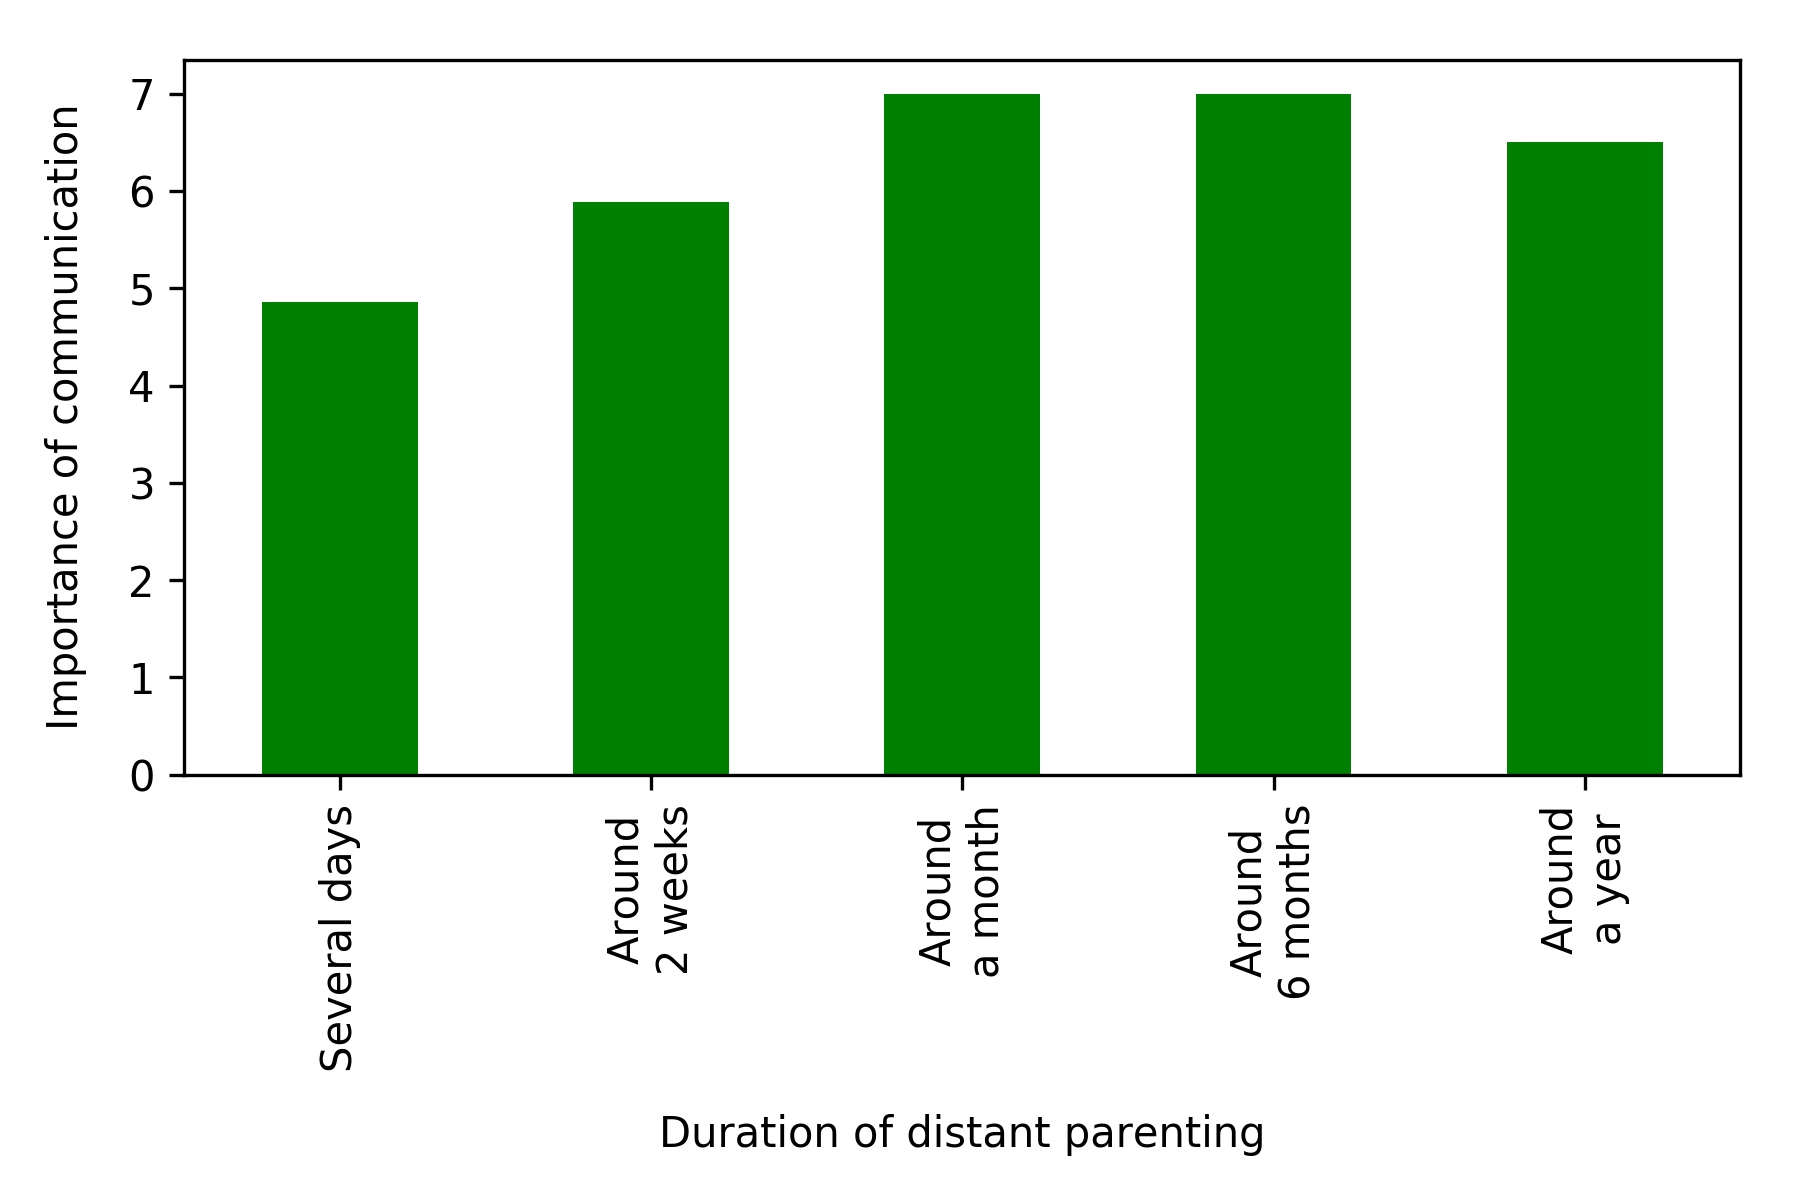
\includegraphics[scale=0.58]{plots/plot_5.png}
    \caption{Importance of communication from the parent point according to duration of distant-parenting experience}
    \label{fig:plot_5}
\end{figure}

\begin{figure}[h!]
    \centering
    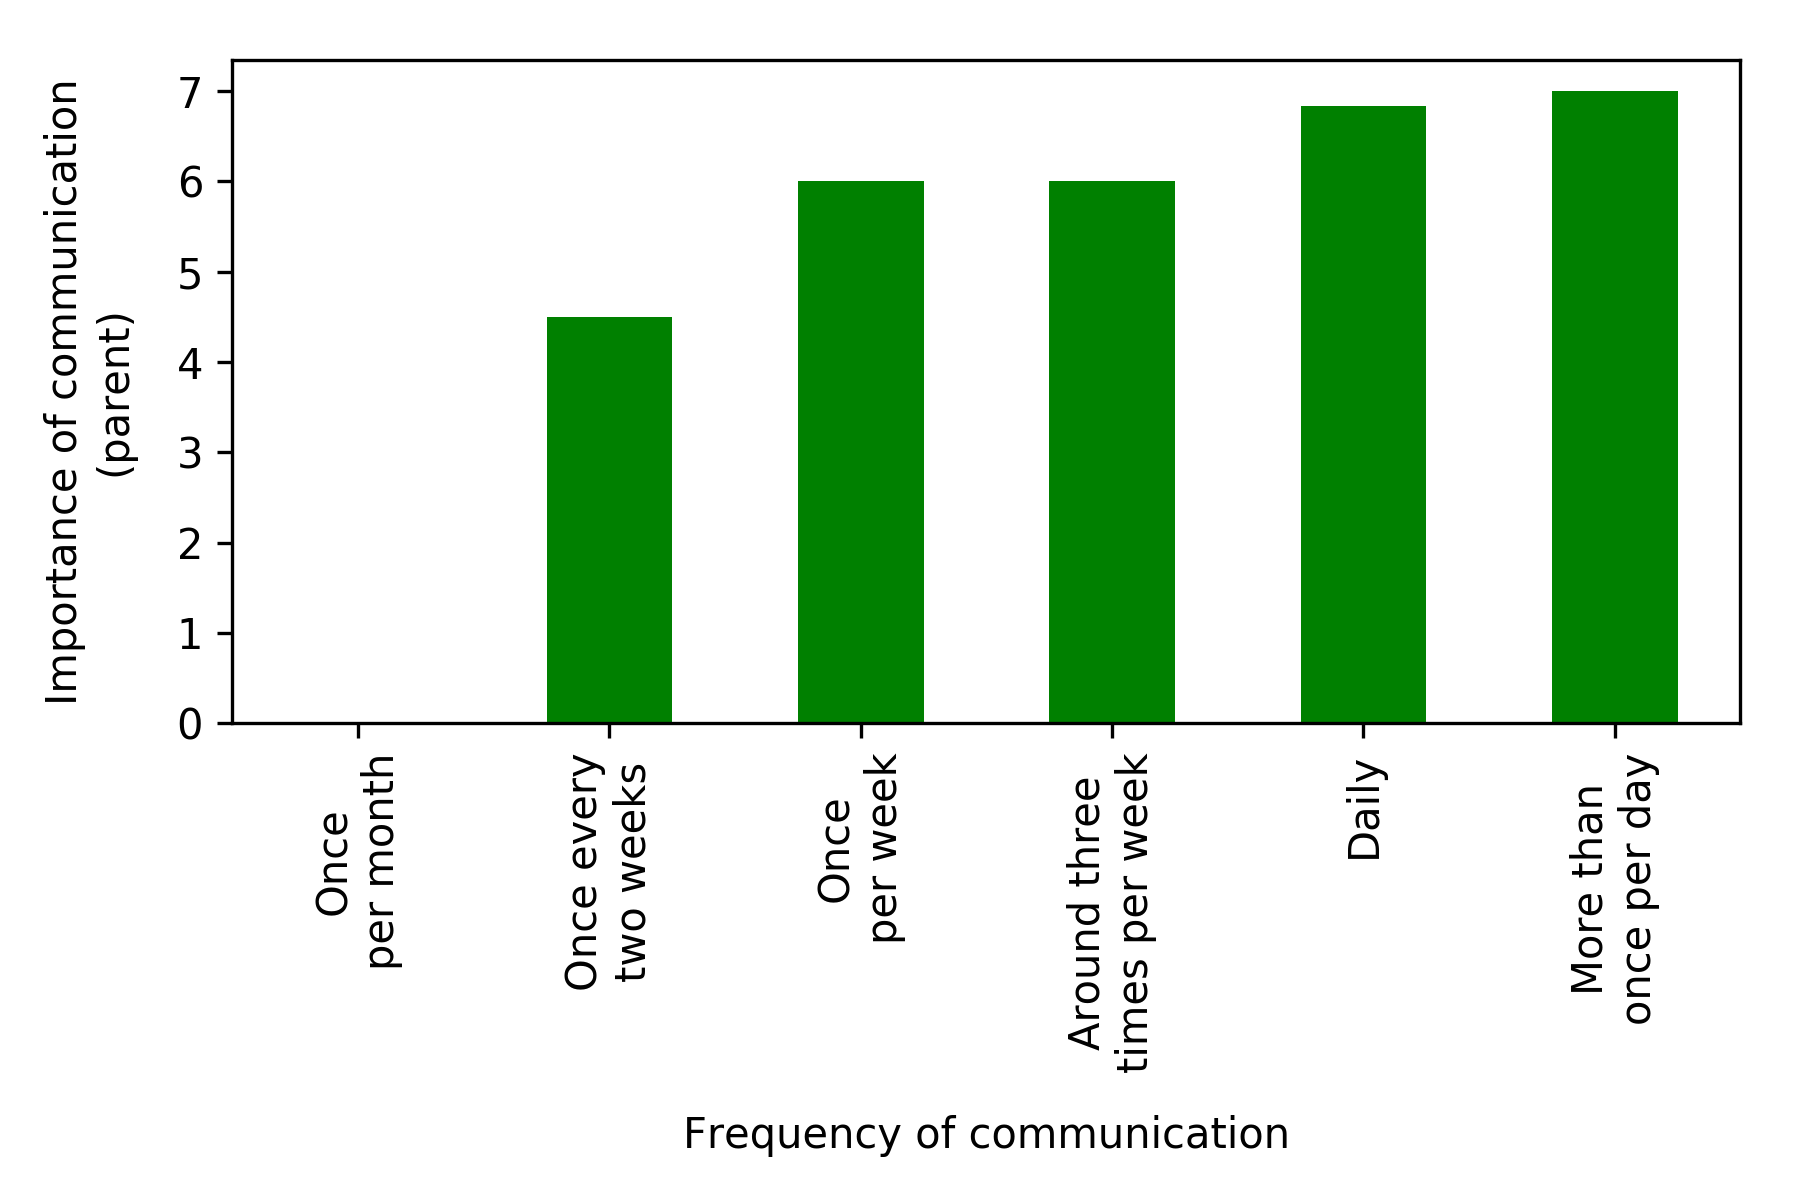
\includegraphics[scale=0.58]{plots/plot_8.png}
    \caption{Importance of communication from the parent point according to frequency of communication during distant-parenting experience}
    \label{fig:plot_8}
\end{figure}


\subsection{Interview protocol}
\label{appendix:interview_protocol}

The following interview protocol has been prepared for the research on “Communication Technologies for Left-Behind Children in Rural China”, in the scope of the “Global perspectives, local realities” SHS course. To continue our research on the Chinese field, by interviewing parents of left behind children, our assumptions could be tested and eventually further analyzed.

\vspace{4pt}
Please, fill in the missing informations as follows before starting the interview session:

Author: Matteo Yann Feo \& Simone Sanso

Session length: 40 minutes 

Participant Name: \hfill \_\_\_\_\_\_\_\_\_\_\_\_\_\_\_\_\_\_\_\_\_\_\_  $\leftarrow$ Fill in

Email: \hfill \_\_\_\_\_\_\_\_\_\_\_\_\_\_\_\_\_\_\_\_\_\_\_\_\_\_\_\_\_\_\_\_ $\leftarrow$ Fill in

Time/Date: \hfill \_\_\_\_\_\_\_\_\_\_\_\_\_\_\_\_\_\_\_\_\_\_\_\_\_\_\_\_ $\leftarrow$ Fill in

Location: \hfill \_\_\_\_\_\_\_\_\_\_\_\_\_\_\_\_\_\_\_\_\_\_\_\_\_\_\_\_\_ $\leftarrow$ Fill in

\vspace{6pt}
\subsubsection{Introduction \& Setup (5 mins)}

The session starts with a short introduction to what this interview is about, the context and the background for which it is being conducted. In the meantime, be sure that everything is setup correctly by double checking the following To-Do list:

\begin{todolist}
    \item Setup the recording tools and check if they work correctly.
    \item Prepare note-taking utilities, such as pen and paper.
    \item Verify the environment, being sure to have a relaxed location for the following 40 mins.
    \item In case a beverage is desired in the meantime, be sure to have it ready and available now.
    \item Be sure that your interviewed person has everything needed.
\end{todolist}

The introduction of the interview could be similar to the following one:

"Good morning and thank you for participating! I am Yann. I am studying at EPFL for a master degree in computer science. My main interest for this interview is to understand whether  a  technology  of  communication embedded in a smart toy could be helpful for parents distant from their children. During the interview, I will be having a conversation with you, asking questions that could help me to achieve my curiosity. In the meantime, my partner, will be assisting me by taking some notes. It is important to always remember that we are not evaluating you or your opinions in any way, there are no possible right and wrong answers that you could give. 
Here is how the session is going to proceed. Firstly, we'll break the ice by asking you a few general questions to know each other. We will record this interview, given your consent. We won't ever share this recording nor use it for anything else but pure support for this interview, so that I can go back and review things later to make sure we got everything right. Your name won't ever be linked to any result, so be relaxed and feel free to share your thoughts with us, without any troubles. Keep in mind that this is completely voluntary, the recording can be stopped whenever you want. Thus, if you don't like this idea, please let me know. 
How does all that sound to you? Do you have any questions at this point?"

\begin{todolist}
    \item Ask the interviewee to sign the written consent for recording purposes.
\end{todolist}

\vspace{2pt}
\subsubsection{Demographics \& Background (5 mins)}

This section will help us to create a background of the interviewee, while allowing him/her to start opening up to our questions. Use this session as a warming-up occasion to break the ice, while catching the first important features. Start to note down details on the interviewee, like gender, age, education level, marital status.

\begin{todolist}
    \item Tell us your name, and a little bit about yourself.
    \item Where do you come from?
    \item What is your occupation? Are you studying or working? In both cases, can you tell us something about it?
    \item Where are you currently living? Do you live with someone, or alone? 
\end{todolist}

\vspace{2pt}
\subsubsection{Main questions (20 mins)}

The following questions can be helpful to interpolate your impressions with the interviewee’s feelings and personal stories. Use them carefully as they might be intimidating for some people. Don’t forget to check for nonverbal behaviors, as they might be critical to have a complete idea of who you are interviewing, especially in this part. Note that the most important questions to be answered are marked with an asterisk (*).

\vspace{2pt}
(*) Pre-interview questions about their children :

\begin{todolist}
    \item How many children do you have?
    \item How old are they?
    \item What gender are they?
    \item Where do you they live?
    \item With who are they staying in your home village? (Lonely, with one of both parents, with grandparents or other relatives)
\end{todolist}

Main interview questions about the interviewed parent :

\begin{todolist}
    \item (*) How often and for how long do you come back home? 
    \item What is the main reason why you live far away from your children?
    \item How do you feel about this situation, not living with your children?
    \item Remember the last time you went back to your home village, how was the contact with your children? Was the meeting with your children as before you left them?
    \item During your childhood, have you ever experienced living far away from one of your parents? If yes, for how long? How did you live the situation? Could you tell us what was the main reason of your parent to out-migrate? How was the contact when meeting again with your parent? Could you communicate together, at that time, while being distant? (Check for non-verbal reactions while interviewee showcase personal experience)
    \item How common is your situation of distant parenting? Do you know any other persons in the same situation as you? How do they live it?
    \item (*) How would you define the importance of living with your children? In your case, is there a trade off between living with your children and having a job position? If yes, imagine that you could live in an ideal world, what would be the best solution? Would you rather work in your home village or be able to bring your children in town?
    \item (*) Do you own electronic devices? If yes, which ones? (Smartphone, computer, more…)
    \item (*) Do your children in your home village own electronic devices? If not, would they have the opportunity to use any? (Neighbourhood, school, etc.)
    \item (*) Do you use electronic devices to contact your children? If yes, how often? In general, are you calling your children when you have time? Or do they also get in touch with you, on their initiative?
    \item (*) From 0 to 7, how would you define the importance of communicating with your children? (0: insignificant, 4: neutral, 7: essential) (Check for non-verbal reactions while interviewee showcase personal experience)
\end{todolist}

\vspace{2pt}
\subsubsection{Interviewee's "show and tell" prototype (8 mins)}

This section is practical and allows us to showcase our project, related to the issue of distant parenting. In the context of CHIC (China Hardware Innovation Camp), a plush toy that encourages social interaction between parents and children, in a distant situation. It is a very resourceful moment, as it could bring additional and authentic feedback on a novel user scenario.

The explanation of the prototype could be similar to the following one:

"We have been working on this prototype. It is a plush toy that encourages social interaction, by having remotely turned on LEDs and sounds from a mobile application. Parents and children can therefore stay longer connected. Letting your children know when you think about them will help you stay 'toygether'\texttrademark."

Showcase the prototype and how it works with the mobile application.

\begin{todolist}
    \item What do you think about the idea?
    \item In your opinion, which are the positive and negative aspects?
    \item If you had the possibility to try this technology, would you be interested?
    \item What would you modify to improve it?
\end{todolist}

\vspace{2pt}
\subsubsection{Closing (2 mins)}

Thank the user at the end for participating to the session. Offer the possibility to ask any kind of question the interviewee might want to address you.  This is his/her time to wear the interviewer's shoes in your regards.

If the interviewee has no additional question, the interview is officially finished. Thank again your interviewee for the time and availability to participate to this session. Underline how useful his/her help has been for the project.
Turn off the recording tools only when you are completely sure that nothing will be added. It is important to not miss anything, so better have some extra recording to cut later.

Take some time to, directly after the end of the interview, write down some impressions you may have about the session. It is important to note down very early impressions about both verbal and physical languages, before they are forgotten. Those are the most authentic resources to get.




\subsection{List of contacts}
\label{appendix:contacts_list}
Below are listed all the contacts that have been reached, to spread as much as possible the survey.

\begin{itemize}
\item AFS programs for adolescents (15-18 years old): \\
Duration: 1 year \\
Kernstrasse 57, CH-8004 Zurich \\
Tel: +41 21 323 19 19 \\
Email: hello@afs.ch \\
https://www.afs.ch/fr/programmes-scolaires/ 

\vspace{4pt}
\item Canada-France exchange (16 years old): \\
Duration : 3 weeks \\
College of Jeanne d'Arc, 15 Rue du Chanoine Brun, 68100 Mulhouse, France \\
Tel: +33 3 89 45 36 31 \\
www.ejda.fr/ 

\vspace{4pt}
\item International exchange programs (14-18 years old): \\
Duration: 1 year \\
Rue Centrale 15, 1003 Lausanne \\
Tel: +41 800 822 811 \\
https://www.efswiss.ch/fr/highschool/ 

\vspace{4pt}
\item National observatory of the Erasmus + impact (1 year or 6 months): \\
Email: observatoire@agence-erasmus.fr \\
http://www.agence-erasmus.fr/page/observatoire/

\vspace{4pt}
\item Journal of international mobility:\\
Email: revue@agence-erasmus.fr \\
https://www.agence-erasmus.fr/page/JIM

\vspace{4pt}
\item Exchange program Brigitte Sauzay (14-17 years old): \\
Duration: 3 months in a host family in Germany and welcome 3 months in the family in France \\
https://www.ofaj.org/contact.html 

\vspace{4pt}
\item Internal exchanges and language stays in Switzerland (14-17 years old): \\
Duration: 1 year \\
College of Delémont, Avenue Station 7, 2800 Delémont \\
Tel: +41 32 421 00 70 \\
Email: info@coldel.org \\
http://www.college-delemont.ch/fr/Aide-aux-eleves/Echanges-et-sejours-linguistiques/Echanges-et-sejours-linguistiques.html \\
Cantonal manager of linguistic exchanges: \\
Patrice KAMBER, Pâquerettes 2, 2822 Courroux \\
- Prof: 032 435 65 92 / Private: 032 422 83 62 

\vspace{4pt}
\item Language Exchange and Mobility - DIP Geneva: \\
Catherine Fernandez Sonino: Head of Exchange \& Mobility DIP of the Cantonal Office for Language Exchange and Mobility \\
Chemin de l'Echo 5a, 1213 Onex \\
Email: catherine.fernandez@etat.ge.ch \\
Tel: +41 22 327 06 43, +41 79 175 56 46 \\
https://edu.ge.ch/site/elem/ 

\vspace{4pt}
\item Service of primary and secondary schools of Lausanne: \\
Place Chauderon 9, 5th floor, PO Box 5032, 1002 Lausanne \\
Tel: +41 21 315 64 11 - Fax: +41 21 315 60 04 \\
Email: seps@lausanne.ch \\
http://www.lausanne.ch/etablissements-scolaires/ 

\vspace{4pt}
\item Summer camp of Neuchatel:\\
Gisèle Nicaty \\
Quartier du Milieu 86, 2127 Les Bayards \\
Tel: +41 79 288 50 41, +41 32 866 17 29\\
Email: giroud.p-a@bluewin.ch\\
http://www.echanges-scolaires.com/index.php/fr/

\vspace{4pt}
\item Summer camp of the Grandes-Roches: \\
1348 le Brassus \\
Tel: +41 21 845 66 90 \\
Email: camps@asime.ch \\
http://www.grandesroches.ch/home 

\vspace{4pt}
\item Association of the Gros-de-Vaud Holiday Camp: \\
Mrs Florence Ethenoz \\
Chemin du Petit Record 60, 1040 Echallens \\
Tel: +41 21 881 10 76 \\
Email: info@colo-gros-de-vaud.ch \\
http://www.colo-gros-de-vaud.ch/clubdesk/www

\vspace{4pt}
\item Summer camp 4Fun: \\
Email: airfred@hotmail.com \\
http://4-fun.ch/ 

\vspace{4pt}
\item Summer camp CPV: \\
Swiss Village Street 14, PO Box 72, 1211 Geneva 8 \\
Tel: +41 22 809 49 79 \\
Email: info@camps.ch \\
http://www.camps.ch/fr/accueil 

\vspace{4pt}
\item Scouts of the Sacred Heart: \\
Jeanne Voruz \& Anne Thiébaud \\
Tel: +41 79 844 92 74 \& +41 79 284 50 38 \\
Email: cg@sacrescout.ch \\
http://www.sacrescout.ch/ 

\vspace{4pt}
\item Village Camps: \\
PO Box 1425, Rue de la Morache 14, 1260 Nyon 1 \\
Tel: +41 22 990 9400 \\
Email: camps@villagecamps.com \\
www.villagecamps.com

\vspace{4pt}
\item Alpadia Language Schools: \\
Grand-Rue 42, PO Box 1206, 1820 Montreux\\
Tel: +41 21 621 88 88\\
Email: info@alpadia.com\\
https://www.alpadia.com/fr/ 

\vspace{4pt}
\item Carol Panchaud Educom sàrl: \\
26 Route of Givrins, CH - 1276 Gingins\\
Tel: +41 22 776 69 15 \\
Email: carolpanchaud@educom.ch \\
http://educom.ch/fr

\vspace{4pt}
\item Caritas-Youth: \\
11, Jean-Violette Street, 1205 Geneva\\
Tel: +41 22 708 04 04\\
Email: info@caritas-jeunesse.ch\\
http://www.caritas-jeunesse.ch/

\vspace{4pt}
\item Holiday Camp St. Gervais: \\
CP 1337, 1211 Geneva 1\\
Tel: +41 78 896 71 84\\
Email: info@colonie-saint-gervais.ch\\
http://www.colonie-saint-gervais.ch/

\vspace{4pt}
\item Summer Camp of Ravoire - Camp Plein Soleil: \\
PO Box 87, CH-1920 Martigny 1\\
Email: info@camp-pleinsoleil.ch

\vspace{4pt}
\item Yverdon-les-Bains youth service and social cohesion: \\
Rue de Neuchâtel 2, 1400 Yverdon-les-Bains\\
Tel: +41 24 423 69 11\\
Email: vacances@yverdon-les-bains.ch\\
http://www.yverdon-les-bains.ch/prestations-deladministration/jeunesse-et-cohesion-sociale/enfanceetfamille/colonies-dete-et-dautomne/

\vspace{4pt}
\item fRilingue GmbH: \\
Stöckackerstrasse 93, 3018 Bern\\
Tel: +41 26 321 34 34 \\
Email: info@frilingue.com

\vspace{4pt}
\item Star Sports: \\
Path of Verger 2, PO Box 101, 1304 Cossonay-Ville\\
Tel: +41 79 356 44 61\\
Email: info@starsports.ch\\
http://www.starsports.ch/

\vspace{4pt}
\item Cap Loisirs Foundation: \\
34, Boulevard de Saint-Georges, 1205 Geneva\\
Tel: +41 22 731 86 00\\
Email: caploisirs@caploisirs.ch\\
http://www.caploisirs.ch/

\vspace{4pt}
\item SCE Holidays \& Events: \\
Rue de Lausanne 58, 1950 Sion\\
Tel: +41 79 693.33.64\\
Email: info@lescamps.ch\\
https://www.lescamps.ch/\\

\end{itemize}



% References of the Report
\thispagestyle{empty}
\vspace{1cm}
\begin{thebibliography}{9}
\addcontentsline{toc}{section}{References}

\bibitem{lab3-report} 
\textit{Lab 3.0 : Camera \& LCD conceptual design}. \\
CS-473 EPFL. Matteo Yann Feo \& Simone Aron Sanso. November 28th, 2017

\bibitem{lcd-controller} 
\textit{ILI9341 - a-Si TFT LCD Single Chip Driver 240RGBx320 Resolution and 262K color}. 
Rev. 1.11. ILI TECHNOLOGY CORP.

\bibitem{lcd-display} 
\textit{LT24 User Manual}. 
Altera. June 2015
 
\bibitem{avalon-interface} 
\textit{Avalon® Interface Specifications}.
MNL-AVABUSREF. Intel. May 2017.
 
\bibitem{fifo} 
\textit{Single- and Dual-Clock FIFO Megafunction}.
Rev. 4.0. Altera. May 2007.

\end{thebibliography}

\end{document}


\documentclass[a4paper,12pt]{article}

%% Layout
\usepackage[utf8]{inputenc}
\usepackage{palatino}
\usepackage[T1]{fontenc}
\usepackage[8pt]{extsizes}

\usepackage{geometry}
\geometry{
    a4paper,
    total={170mm,257mm},
    left=30mm,
    right=30mm,
    top=30mm,
    bottom=30mm,
 } 

%% Useful packages
\usepackage{amsmath}
\usepackage{amssymb}
\usepackage{mathtools}
\usepackage{microtype}

\usepackage[usenames, dvipsnames]{xcolor}
\usepackage{graphicx}
\usepackage{wrapfig}
\usepackage{subfig}
\usepackage{tabularx}
\usepackage{float}
\usepackage{caption}
\usepackage{multirow}
\usepackage{color, colortbl}
\usepackage{enumerate}

\usepackage{hyperref}
\usepackage{url}

\usepackage[english]{babel}
\usepackage{units}

\usepackage{textcomp}
\usepackage{titling}
\usepackage{blindtext}
\usepackage{listings}

\usepackage{braket}
\usepackage{rotating}

%\setlength{\droptitle}{-4em}     % Eliminate the default vertical space
%\addtolength{\droptitle}{-4pt}

\title{
    \centering
	
\includegraphics[width=0.5\textwidth]{images/Logo_EPFL.png}
    \\[1cm]
	\Huge China Hardware Innovation Camp\\[1cm]
    \huge Semester project report\\
    \rule{3.5cm}{0.9pt}\\[0.5cm]
    \huge HUM - 498 \vfill
    \normalsize
}

\author{
    \textbf{Laboratory group:}\\\\
    Chloe Dickson - \texttt{\href{mailto:chloe.dickson@epfl.ch}{simone.sanso@epfl.ch}} \\
    Matteo Yann Feo -    \texttt{\href{mailto:matteo.feo@epfl.ch}{matteo.feo@epfl.ch}} \\
    Simone Aron Sanso - \texttt{\href{mailto:simone.sanso@epfl.ch}{simone.sanso@epfl.ch}} \\\\
}

\date{\vfill \today}

\lstdefinestyle{Python}{
  language=Python,                % choose the language of the code
  numbers=left,                   % where to put the line-numbers
  stepnumber=1,                   % the step between two line-numbers.        
  numbersep=5pt,                  % how far the line-numbers are from the code
  backgroundcolor=\color{white},  % choose the background color. You must add \usepackage{color}
  showspaces=false,               % show spaces adding particular underscores
  showstringspaces=false,         % underline spaces within strings
  showtabs=false,                 % show tabs within strings adding particular underscores
  tabsize=2,                      % sets default tabsize to 2 spaces
  captionpos=b,                   % sets the caption-position to bottom
  breaklines=true,                % sets automatic line breaking
  breakatwhitespace=true,         % sets if automatic breaks should only happen at whitespace
  frame=single, 
  basicstyle=\ttfamily,
  keywordstyle=\color{Green}\bfseries,
  stringstyle=\color{red}\ttfamily,
  commentstyle=\color{OliveGreen}\ttfamily,
  %morecomment=[l][\color{magenta}]{\#}
}


\begin{document}
\maketitle
\thispagestyle{empty}

\newpage
\thispagestyle{empty}
\setcounter{page}{0}

\tableofcontents

\documentclass[a4paper,12pt]{article}

%% Layout
\usepackage[utf8]{inputenc}
\usepackage{palatino}
\usepackage[T1]{fontenc}
\usepackage[8pt]{extsizes}

\usepackage{geometry}
\geometry{
    a4paper,
    total={170mm,257mm},
    left=30mm,
    right=30mm,
    top=30mm,
    bottom=30mm,
 } 

%% Useful packages
\usepackage{amsmath}
\usepackage{amssymb}
\usepackage{mathtools}
\usepackage{microtype}

\usepackage[usenames, dvipsnames]{xcolor}
\usepackage{graphicx}
\usepackage{wrapfig}
\usepackage{subfig}
\usepackage{tabularx}
\usepackage{float}
\usepackage{caption}
\usepackage{multirow}
\usepackage{color, colortbl}
\usepackage{enumerate}

\usepackage{hyperref}
\usepackage{url}

\usepackage[english]{babel}
\usepackage{units}

\usepackage{textcomp}
\usepackage{titling}
\usepackage{blindtext}
\usepackage{listings}

\usepackage{braket}
\usepackage{rotating}

%\setlength{\droptitle}{-4em}     % Eliminate the default vertical space
%\addtolength{\droptitle}{-4pt}

\title{
    \centering
	
\includegraphics[width=0.5\textwidth]{images/Logo_EPFL.png}
    \\[1cm]
	\Huge China Hardware Innovation Camp\\[1cm]
    \huge Semester project report\\
    \rule{3.5cm}{0.9pt}\\[0.5cm]
    \huge HUM - 498 \vfill
    \normalsize
}

\author{
    \textbf{Laboratory group:}\\\\
    Chloe Dickson - \texttt{\href{mailto:chloe.dickson@epfl.ch}{simone.sanso@epfl.ch}} \\
    Matteo Yann Feo -    \texttt{\href{mailto:matteo.feo@epfl.ch}{matteo.feo@epfl.ch}} \\
    Simone Aron Sanso - \texttt{\href{mailto:simone.sanso@epfl.ch}{simone.sanso@epfl.ch}} \\\\
}

\date{\vfill \today}

\lstdefinestyle{Python}{
  language=Python,                % choose the language of the code
  numbers=left,                   % where to put the line-numbers
  stepnumber=1,                   % the step between two line-numbers.        
  numbersep=5pt,                  % how far the line-numbers are from the code
  backgroundcolor=\color{white},  % choose the background color. You must add \usepackage{color}
  showspaces=false,               % show spaces adding particular underscores
  showstringspaces=false,         % underline spaces within strings
  showtabs=false,                 % show tabs within strings adding particular underscores
  tabsize=2,                      % sets default tabsize to 2 spaces
  captionpos=b,                   % sets the caption-position to bottom
  breaklines=true,                % sets automatic line breaking
  breakatwhitespace=true,         % sets if automatic breaks should only happen at whitespace
  frame=single, 
  basicstyle=\ttfamily,
  keywordstyle=\color{Green}\bfseries,
  stringstyle=\color{red}\ttfamily,
  commentstyle=\color{OliveGreen}\ttfamily,
  %morecomment=[l][\color{magenta}]{\#}
}


\begin{document}
\maketitle
\thispagestyle{empty}

\newpage
\thispagestyle{empty}
\setcounter{page}{0}

\tableofcontents

\input{sections/1_introduction/main.tex}

\input{sections/2_structure/main.tex}
    \input{sections/2_structure/subsection_A.tex}
    \input{sections/2_structure/subsection_B.tex}
    \input{sections/2_structure/subsection_C.tex}
    
\input{sections/3_images_tables/main.tex}

\input{sections/4_code/main.tex}

\input{sections/5_conclusion/main.tex}

\input{appendix.tex}

\input{bibliography.tex}

\end{document}


\documentclass[a4paper,12pt]{article}

%% Layout
\usepackage[utf8]{inputenc}
\usepackage{palatino}
\usepackage[T1]{fontenc}
\usepackage[8pt]{extsizes}

\usepackage{geometry}
\geometry{
    a4paper,
    total={170mm,257mm},
    left=30mm,
    right=30mm,
    top=30mm,
    bottom=30mm,
 } 

%% Useful packages
\usepackage{amsmath}
\usepackage{amssymb}
\usepackage{mathtools}
\usepackage{microtype}

\usepackage[usenames, dvipsnames]{xcolor}
\usepackage{graphicx}
\usepackage{wrapfig}
\usepackage{subfig}
\usepackage{tabularx}
\usepackage{float}
\usepackage{caption}
\usepackage{multirow}
\usepackage{color, colortbl}
\usepackage{enumerate}

\usepackage{hyperref}
\usepackage{url}

\usepackage[english]{babel}
\usepackage{units}

\usepackage{textcomp}
\usepackage{titling}
\usepackage{blindtext}
\usepackage{listings}

\usepackage{braket}
\usepackage{rotating}

%\setlength{\droptitle}{-4em}     % Eliminate the default vertical space
%\addtolength{\droptitle}{-4pt}

\title{
    \centering
	
\includegraphics[width=0.5\textwidth]{images/Logo_EPFL.png}
    \\[1cm]
	\Huge China Hardware Innovation Camp\\[1cm]
    \huge Semester project report\\
    \rule{3.5cm}{0.9pt}\\[0.5cm]
    \huge HUM - 498 \vfill
    \normalsize
}

\author{
    \textbf{Laboratory group:}\\\\
    Chloe Dickson - \texttt{\href{mailto:chloe.dickson@epfl.ch}{simone.sanso@epfl.ch}} \\
    Matteo Yann Feo -    \texttt{\href{mailto:matteo.feo@epfl.ch}{matteo.feo@epfl.ch}} \\
    Simone Aron Sanso - \texttt{\href{mailto:simone.sanso@epfl.ch}{simone.sanso@epfl.ch}} \\\\
}

\date{\vfill \today}

\lstdefinestyle{Python}{
  language=Python,                % choose the language of the code
  numbers=left,                   % where to put the line-numbers
  stepnumber=1,                   % the step between two line-numbers.        
  numbersep=5pt,                  % how far the line-numbers are from the code
  backgroundcolor=\color{white},  % choose the background color. You must add \usepackage{color}
  showspaces=false,               % show spaces adding particular underscores
  showstringspaces=false,         % underline spaces within strings
  showtabs=false,                 % show tabs within strings adding particular underscores
  tabsize=2,                      % sets default tabsize to 2 spaces
  captionpos=b,                   % sets the caption-position to bottom
  breaklines=true,                % sets automatic line breaking
  breakatwhitespace=true,         % sets if automatic breaks should only happen at whitespace
  frame=single, 
  basicstyle=\ttfamily,
  keywordstyle=\color{Green}\bfseries,
  stringstyle=\color{red}\ttfamily,
  commentstyle=\color{OliveGreen}\ttfamily,
  %morecomment=[l][\color{magenta}]{\#}
}


\begin{document}
\maketitle
\thispagestyle{empty}

\newpage
\thispagestyle{empty}
\setcounter{page}{0}

\tableofcontents

\input{sections/1_introduction/main.tex}

\input{sections/2_structure/main.tex}
    \input{sections/2_structure/subsection_A.tex}
    \input{sections/2_structure/subsection_B.tex}
    \input{sections/2_structure/subsection_C.tex}
    
\input{sections/3_images_tables/main.tex}

\input{sections/4_code/main.tex}

\input{sections/5_conclusion/main.tex}

\input{appendix.tex}

\input{bibliography.tex}

\end{document}

    %\newpage
\subsection{Subsection A}
\label{subsec:A} 

This is the first subsection. I am saved into a file \textit{subsection\_A.tex} in the same folder as my main file. Pay attention to the format in the label tag in order to reference to the subsection elsewhere. The subsection is called in the main file of the whole document !

\medskip Nunc pulvinar, risus sed gravida pretium, eros tellus vehicula turpis, eget bibendum nisi dolor sed erat. Pellentesque sit amet orci sed ligula dictum cursus. Morbi gravida ligula sapien, non tristique orci semper id. Ut sollicitudin est ut nisi eleifend sollicitudin. Vivamus blandit congue risus id porttitor. Donec sed blandit mauris. Integer est leo, dapibus sed felis et, vulputate sagittis enim. Quisque eget purus vitae metus placerat rhoncus. Nulla eget lacus nec felis tincidunt suscipit ac eget tellus. Ut at augue fermentum, mattis justo sed, consectetur quam. Donec blandit euismod nisi ac auctor.
    %\newpage
\subsection{Subsection B}
\label{subsec:B} 

This is the second subsection. I am also saved into a file \textit{subsection\_B.tex} in the same folder as my main file. Pay attention to the format in the label tag in order to reference to the subsection elsewhere. The subsection is called in the main file of the whole document !

\medskip Nunc pulvinar, risus sed gravida pretium, eros tellus vehicula turpis, eget bibendum nisi dolor sed erat. Pellentesque sit amet orci sed ligula dictum cursus. Morbi gravida ligula sapien, non tristique orci semper id. Ut sollicitudin est ut nisi eleifend sollicitudin. Vivamus blandit congue risus id porttitor. Donec sed blandit mauris. Integer est leo, dapibus sed felis et, vulputate sagittis enim. Quisque eget purus vitae metus placerat rhoncus. Nulla eget lacus nec felis tincidunt suscipit ac eget tellus. Ut at augue fermentum, mattis justo sed, consectetur quam. Donec blandit euismod nisi ac auctor.
    %\newpage
\subsection{Subsection C}
\label{subsec:C} 

Okay, you got it by now ;-)
    
\documentclass[a4paper,12pt]{article}

%% Layout
\usepackage[utf8]{inputenc}
\usepackage{palatino}
\usepackage[T1]{fontenc}
\usepackage[8pt]{extsizes}

\usepackage{geometry}
\geometry{
    a4paper,
    total={170mm,257mm},
    left=30mm,
    right=30mm,
    top=30mm,
    bottom=30mm,
 } 

%% Useful packages
\usepackage{amsmath}
\usepackage{amssymb}
\usepackage{mathtools}
\usepackage{microtype}

\usepackage[usenames, dvipsnames]{xcolor}
\usepackage{graphicx}
\usepackage{wrapfig}
\usepackage{subfig}
\usepackage{tabularx}
\usepackage{float}
\usepackage{caption}
\usepackage{multirow}
\usepackage{color, colortbl}
\usepackage{enumerate}

\usepackage{hyperref}
\usepackage{url}

\usepackage[english]{babel}
\usepackage{units}

\usepackage{textcomp}
\usepackage{titling}
\usepackage{blindtext}
\usepackage{listings}

\usepackage{braket}
\usepackage{rotating}

%\setlength{\droptitle}{-4em}     % Eliminate the default vertical space
%\addtolength{\droptitle}{-4pt}

\title{
    \centering
	
\includegraphics[width=0.5\textwidth]{images/Logo_EPFL.png}
    \\[1cm]
	\Huge China Hardware Innovation Camp\\[1cm]
    \huge Semester project report\\
    \rule{3.5cm}{0.9pt}\\[0.5cm]
    \huge HUM - 498 \vfill
    \normalsize
}

\author{
    \textbf{Laboratory group:}\\\\
    Chloe Dickson - \texttt{\href{mailto:chloe.dickson@epfl.ch}{simone.sanso@epfl.ch}} \\
    Matteo Yann Feo -    \texttt{\href{mailto:matteo.feo@epfl.ch}{matteo.feo@epfl.ch}} \\
    Simone Aron Sanso - \texttt{\href{mailto:simone.sanso@epfl.ch}{simone.sanso@epfl.ch}} \\\\
}

\date{\vfill \today}

\lstdefinestyle{Python}{
  language=Python,                % choose the language of the code
  numbers=left,                   % where to put the line-numbers
  stepnumber=1,                   % the step between two line-numbers.        
  numbersep=5pt,                  % how far the line-numbers are from the code
  backgroundcolor=\color{white},  % choose the background color. You must add \usepackage{color}
  showspaces=false,               % show spaces adding particular underscores
  showstringspaces=false,         % underline spaces within strings
  showtabs=false,                 % show tabs within strings adding particular underscores
  tabsize=2,                      % sets default tabsize to 2 spaces
  captionpos=b,                   % sets the caption-position to bottom
  breaklines=true,                % sets automatic line breaking
  breakatwhitespace=true,         % sets if automatic breaks should only happen at whitespace
  frame=single, 
  basicstyle=\ttfamily,
  keywordstyle=\color{Green}\bfseries,
  stringstyle=\color{red}\ttfamily,
  commentstyle=\color{OliveGreen}\ttfamily,
  %morecomment=[l][\color{magenta}]{\#}
}


\begin{document}
\maketitle
\thispagestyle{empty}

\newpage
\thispagestyle{empty}
\setcounter{page}{0}

\tableofcontents

\input{sections/1_introduction/main.tex}

\input{sections/2_structure/main.tex}
    \input{sections/2_structure/subsection_A.tex}
    \input{sections/2_structure/subsection_B.tex}
    \input{sections/2_structure/subsection_C.tex}
    
\input{sections/3_images_tables/main.tex}

\input{sections/4_code/main.tex}

\input{sections/5_conclusion/main.tex}

\input{appendix.tex}

\input{bibliography.tex}

\end{document}


\documentclass[a4paper,12pt]{article}

%% Layout
\usepackage[utf8]{inputenc}
\usepackage{palatino}
\usepackage[T1]{fontenc}
\usepackage[8pt]{extsizes}

\usepackage{geometry}
\geometry{
    a4paper,
    total={170mm,257mm},
    left=30mm,
    right=30mm,
    top=30mm,
    bottom=30mm,
 } 

%% Useful packages
\usepackage{amsmath}
\usepackage{amssymb}
\usepackage{mathtools}
\usepackage{microtype}

\usepackage[usenames, dvipsnames]{xcolor}
\usepackage{graphicx}
\usepackage{wrapfig}
\usepackage{subfig}
\usepackage{tabularx}
\usepackage{float}
\usepackage{caption}
\usepackage{multirow}
\usepackage{color, colortbl}
\usepackage{enumerate}

\usepackage{hyperref}
\usepackage{url}

\usepackage[english]{babel}
\usepackage{units}

\usepackage{textcomp}
\usepackage{titling}
\usepackage{blindtext}
\usepackage{listings}

\usepackage{braket}
\usepackage{rotating}

%\setlength{\droptitle}{-4em}     % Eliminate the default vertical space
%\addtolength{\droptitle}{-4pt}

\title{
    \centering
	
\includegraphics[width=0.5\textwidth]{images/Logo_EPFL.png}
    \\[1cm]
	\Huge China Hardware Innovation Camp\\[1cm]
    \huge Semester project report\\
    \rule{3.5cm}{0.9pt}\\[0.5cm]
    \huge HUM - 498 \vfill
    \normalsize
}

\author{
    \textbf{Laboratory group:}\\\\
    Chloe Dickson - \texttt{\href{mailto:chloe.dickson@epfl.ch}{simone.sanso@epfl.ch}} \\
    Matteo Yann Feo -    \texttt{\href{mailto:matteo.feo@epfl.ch}{matteo.feo@epfl.ch}} \\
    Simone Aron Sanso - \texttt{\href{mailto:simone.sanso@epfl.ch}{simone.sanso@epfl.ch}} \\\\
}

\date{\vfill \today}

\lstdefinestyle{Python}{
  language=Python,                % choose the language of the code
  numbers=left,                   % where to put the line-numbers
  stepnumber=1,                   % the step between two line-numbers.        
  numbersep=5pt,                  % how far the line-numbers are from the code
  backgroundcolor=\color{white},  % choose the background color. You must add \usepackage{color}
  showspaces=false,               % show spaces adding particular underscores
  showstringspaces=false,         % underline spaces within strings
  showtabs=false,                 % show tabs within strings adding particular underscores
  tabsize=2,                      % sets default tabsize to 2 spaces
  captionpos=b,                   % sets the caption-position to bottom
  breaklines=true,                % sets automatic line breaking
  breakatwhitespace=true,         % sets if automatic breaks should only happen at whitespace
  frame=single, 
  basicstyle=\ttfamily,
  keywordstyle=\color{Green}\bfseries,
  stringstyle=\color{red}\ttfamily,
  commentstyle=\color{OliveGreen}\ttfamily,
  %morecomment=[l][\color{magenta}]{\#}
}


\begin{document}
\maketitle
\thispagestyle{empty}

\newpage
\thispagestyle{empty}
\setcounter{page}{0}

\tableofcontents

\input{sections/1_introduction/main.tex}

\input{sections/2_structure/main.tex}
    \input{sections/2_structure/subsection_A.tex}
    \input{sections/2_structure/subsection_B.tex}
    \input{sections/2_structure/subsection_C.tex}
    
\input{sections/3_images_tables/main.tex}

\input{sections/4_code/main.tex}

\input{sections/5_conclusion/main.tex}

\input{appendix.tex}

\input{bibliography.tex}

\end{document}


\documentclass[a4paper,12pt]{article}

%% Layout
\usepackage[utf8]{inputenc}
\usepackage{palatino}
\usepackage[T1]{fontenc}
\usepackage[8pt]{extsizes}

\usepackage{geometry}
\geometry{
    a4paper,
    total={170mm,257mm},
    left=30mm,
    right=30mm,
    top=30mm,
    bottom=30mm,
 } 

%% Useful packages
\usepackage{amsmath}
\usepackage{amssymb}
\usepackage{mathtools}
\usepackage{microtype}

\usepackage[usenames, dvipsnames]{xcolor}
\usepackage{graphicx}
\usepackage{wrapfig}
\usepackage{subfig}
\usepackage{tabularx}
\usepackage{float}
\usepackage{caption}
\usepackage{multirow}
\usepackage{color, colortbl}
\usepackage{enumerate}

\usepackage{hyperref}
\usepackage{url}

\usepackage[english]{babel}
\usepackage{units}

\usepackage{textcomp}
\usepackage{titling}
\usepackage{blindtext}
\usepackage{listings}

\usepackage{braket}
\usepackage{rotating}

%\setlength{\droptitle}{-4em}     % Eliminate the default vertical space
%\addtolength{\droptitle}{-4pt}

\title{
    \centering
	
\includegraphics[width=0.5\textwidth]{images/Logo_EPFL.png}
    \\[1cm]
	\Huge China Hardware Innovation Camp\\[1cm]
    \huge Semester project report\\
    \rule{3.5cm}{0.9pt}\\[0.5cm]
    \huge HUM - 498 \vfill
    \normalsize
}

\author{
    \textbf{Laboratory group:}\\\\
    Chloe Dickson - \texttt{\href{mailto:chloe.dickson@epfl.ch}{simone.sanso@epfl.ch}} \\
    Matteo Yann Feo -    \texttt{\href{mailto:matteo.feo@epfl.ch}{matteo.feo@epfl.ch}} \\
    Simone Aron Sanso - \texttt{\href{mailto:simone.sanso@epfl.ch}{simone.sanso@epfl.ch}} \\\\
}

\date{\vfill \today}

\lstdefinestyle{Python}{
  language=Python,                % choose the language of the code
  numbers=left,                   % where to put the line-numbers
  stepnumber=1,                   % the step between two line-numbers.        
  numbersep=5pt,                  % how far the line-numbers are from the code
  backgroundcolor=\color{white},  % choose the background color. You must add \usepackage{color}
  showspaces=false,               % show spaces adding particular underscores
  showstringspaces=false,         % underline spaces within strings
  showtabs=false,                 % show tabs within strings adding particular underscores
  tabsize=2,                      % sets default tabsize to 2 spaces
  captionpos=b,                   % sets the caption-position to bottom
  breaklines=true,                % sets automatic line breaking
  breakatwhitespace=true,         % sets if automatic breaks should only happen at whitespace
  frame=single, 
  basicstyle=\ttfamily,
  keywordstyle=\color{Green}\bfseries,
  stringstyle=\color{red}\ttfamily,
  commentstyle=\color{OliveGreen}\ttfamily,
  %morecomment=[l][\color{magenta}]{\#}
}


\begin{document}
\maketitle
\thispagestyle{empty}

\newpage
\thispagestyle{empty}
\setcounter{page}{0}

\tableofcontents

\input{sections/1_introduction/main.tex}

\input{sections/2_structure/main.tex}
    \input{sections/2_structure/subsection_A.tex}
    \input{sections/2_structure/subsection_B.tex}
    \input{sections/2_structure/subsection_C.tex}
    
\input{sections/3_images_tables/main.tex}

\input{sections/4_code/main.tex}

\input{sections/5_conclusion/main.tex}

\input{appendix.tex}

\input{bibliography.tex}

\end{document}


% Appendix of the Report
\appendix

In the following appendix are presented the questions of the survey (... a list of figures and tables) to the reader.

\subsection{Questions of the survey}
\label{appendix:survey_questions}
In this section is shown how the participants were questioned towards the survey. Only the questions in English will be shown here, skipping the French translations.

\medskip \textit{Form about communication technologies :} \\
Realizing a research project about social sciences within EPFL University (Lausanne), we would like to understand the importance of communication between parents and children, when they are at a distance during a continuous period of time.

\vspace{4pt}
1. In what language would like to answer this form?

2. To contextualize, we seek either :

- parents of a child having spent a period of time away from the household,

- children, teenagers and young adults having spent a period of time away from their family.

After having read the description above, do you qualify yourself as a parent or a child?

\vspace{4pt}
\noindent - If "parent" was selected question 2: 

3.a. Are you the mother or the father?

4.a. Have you already been separated from your child for at least 3 days? (Exchange semester abroad, holidays, summer camp, boy-scout, etc.)

5.a. If there were more than one experience of distance parenting, please consider the earliest one of them through the rest of the form (when you were the youngest). What is the reason why your child was distant from you? 

6.a. For how long have you been distant from your child?

7.a. How old was your child at that time?

8.a. What is your child's gender?

9.a. How often did you use a communication technology with your distant child? (Text messages, phone calls, video chat, etc.)

10.a. What kind of information did you seek from communicating with your distant child?

11.a. How would you define the importance of being able to communicate with your distant child?

\vspace{4pt}
\noindent - If "child" was selected question 2: 

3.b. Have you already been separated from your family for at least 3 days? (Exchange semester abroad, holidays, summer camp, boy-scout, etc.)

3.b. If there were more than one experience of separation from your family, please consider the earliest one of them through the rest of the form (when you were the youngest). What is the reason why you were distant from your family? 

4.b. For how long have you been away?

5.b. How old were you at that time?

6.b. What is your gender?

7.b. How often did you use a communication technology with your family? (Text messages, phone calls, video chat, etc.)

8.b. What kind of information did you seek from communicating with your family?

9.b. How would you define the importance of being able to communicate with your family?


\subsection{Additional plots of the results}
\label{appendix:additional-plots}

The following plots have been computed for the analysis of the data collected via the survey on distant-parenting. This appendix contains a set of plots that didn't need particular attention during the discussion, but can still be source of investigation.

\begin{figure}[h!]
    \centering
    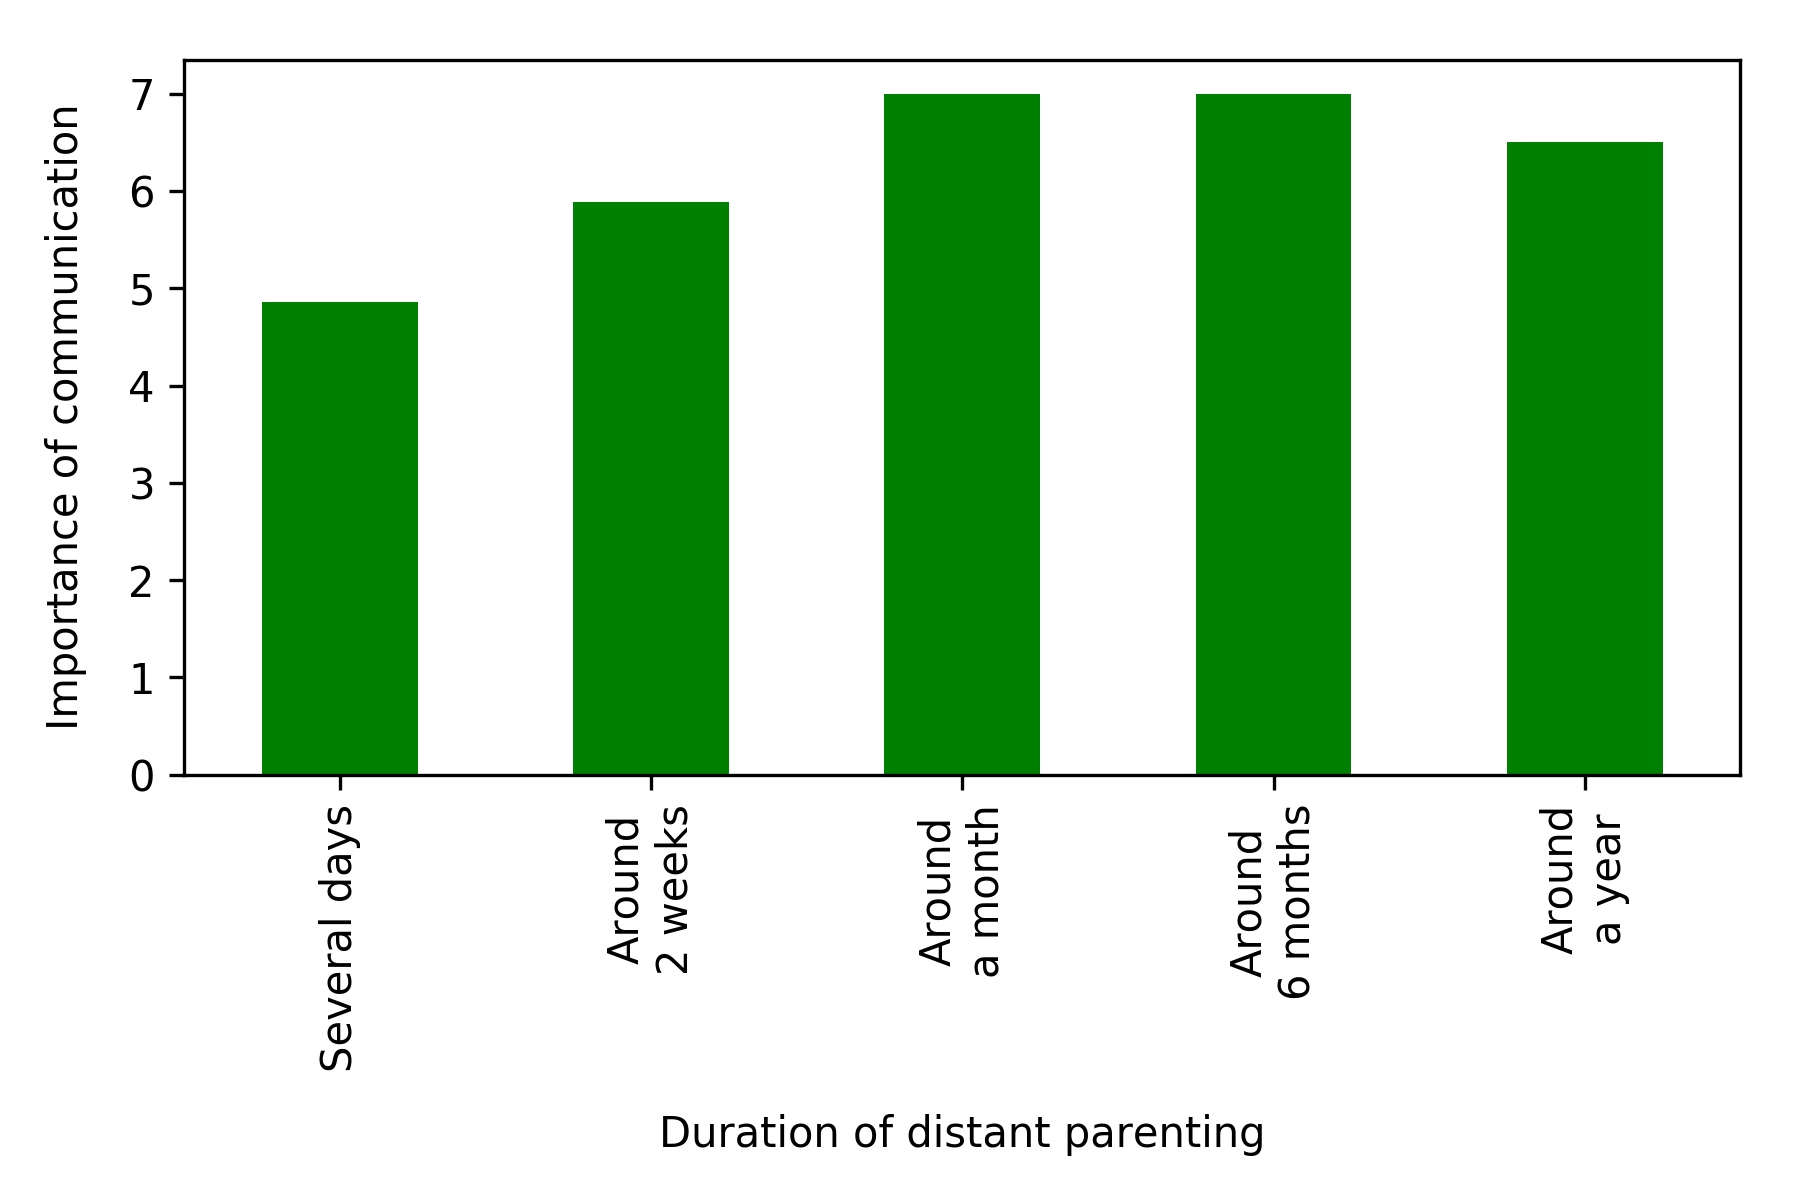
\includegraphics[scale=0.58]{plots/plot_5.png}
    \caption{Importance of communication from the parent point according to duration of distant-parenting experience}
    \label{fig:plot_5}
\end{figure}

\begin{figure}[h!]
    \centering
    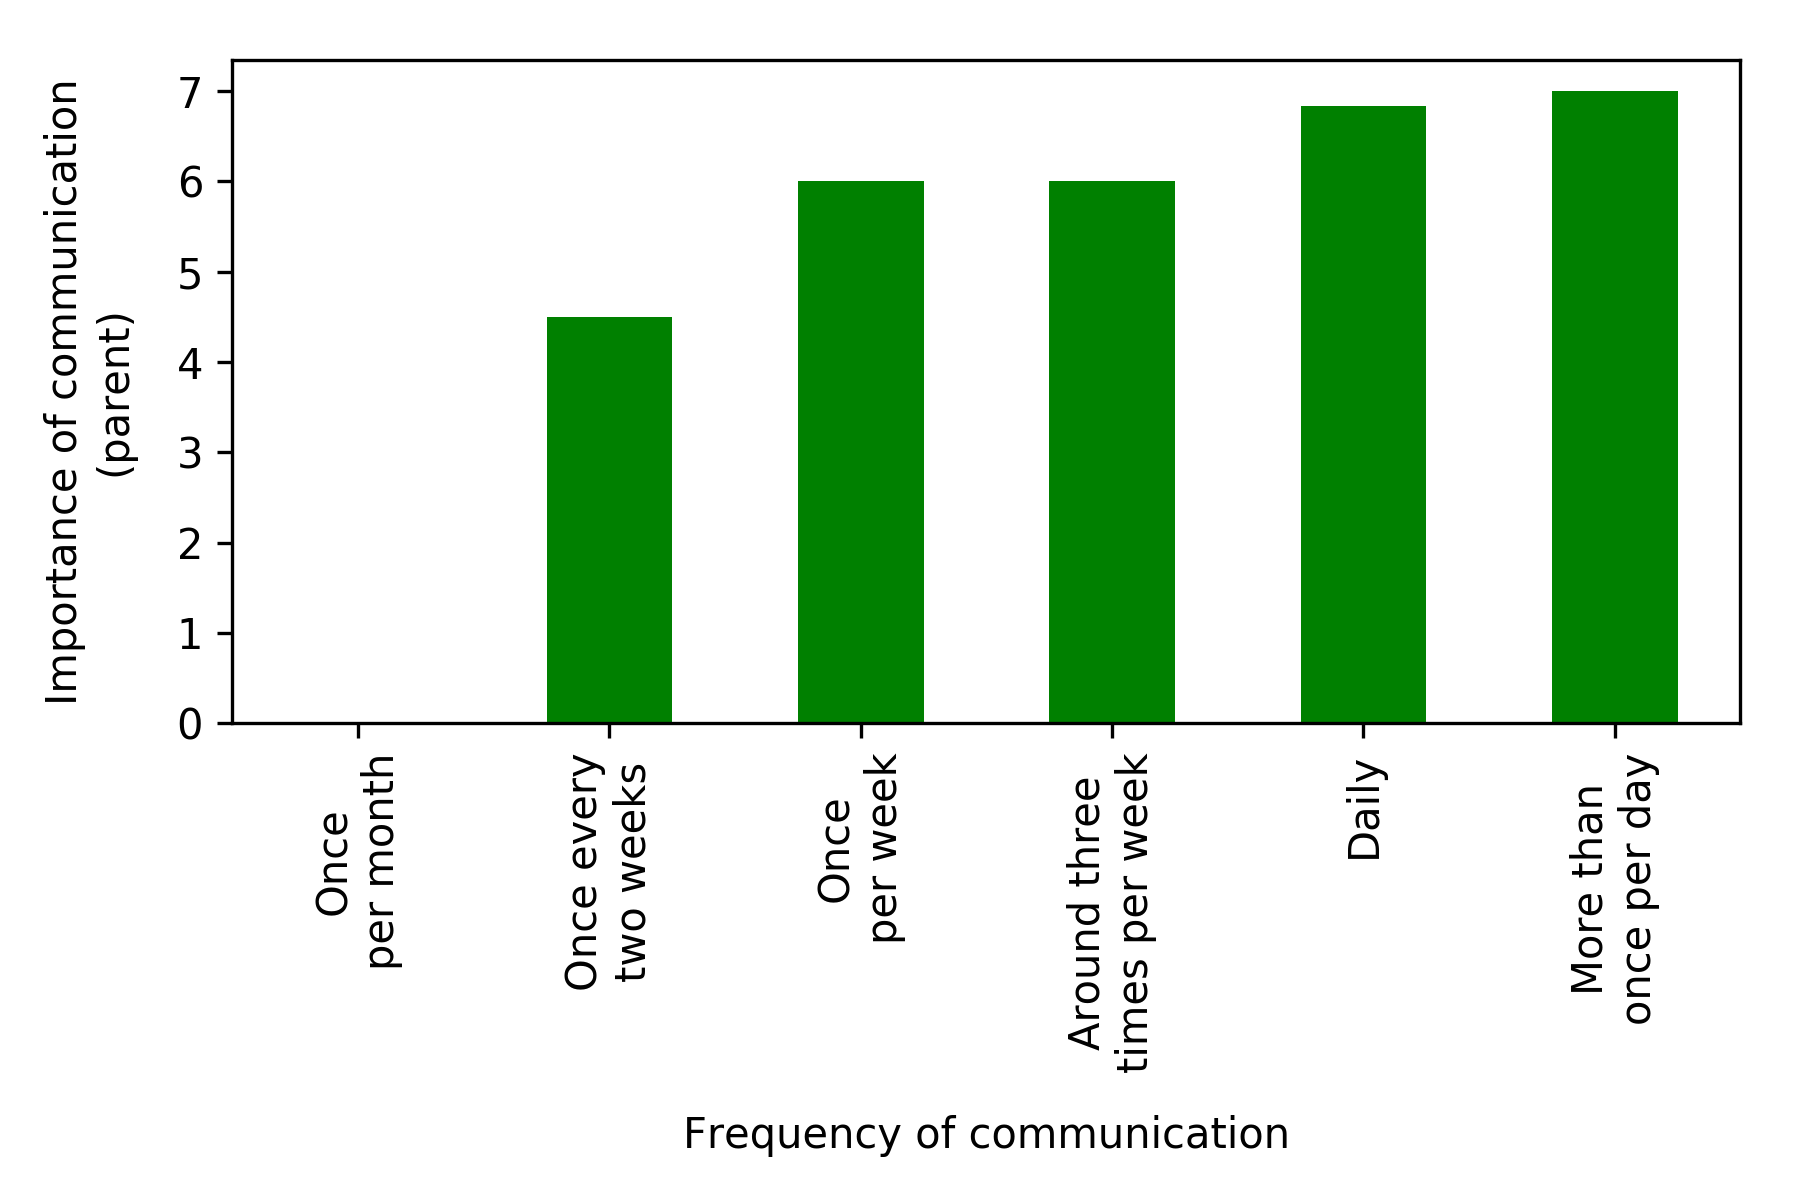
\includegraphics[scale=0.58]{plots/plot_8.png}
    \caption{Importance of communication from the parent point according to frequency of communication during distant-parenting experience}
    \label{fig:plot_8}
\end{figure}


\subsection{Interview protocol}
\label{appendix:interview_protocol}

The following interview protocol has been prepared for the research on “Communication Technologies for Left-Behind Children in Rural China”, in the scope of the “Global perspectives, local realities” SHS course. To continue our research on the Chinese field, by interviewing parents of left behind children, our assumptions could be tested and eventually further analyzed.

\vspace{4pt}
Please, fill in the missing informations as follows before starting the interview session:

Author: Matteo Yann Feo \& Simone Sanso

Session length: 40 minutes 

Participant Name: \hfill \_\_\_\_\_\_\_\_\_\_\_\_\_\_\_\_\_\_\_\_\_\_\_  $\leftarrow$ Fill in

Email: \hfill \_\_\_\_\_\_\_\_\_\_\_\_\_\_\_\_\_\_\_\_\_\_\_\_\_\_\_\_\_\_\_\_ $\leftarrow$ Fill in

Time/Date: \hfill \_\_\_\_\_\_\_\_\_\_\_\_\_\_\_\_\_\_\_\_\_\_\_\_\_\_\_\_ $\leftarrow$ Fill in

Location: \hfill \_\_\_\_\_\_\_\_\_\_\_\_\_\_\_\_\_\_\_\_\_\_\_\_\_\_\_\_\_ $\leftarrow$ Fill in

\vspace{6pt}
\subsubsection{Introduction \& Setup (5 mins)}

The session starts with a short introduction to what this interview is about, the context and the background for which it is being conducted. In the meantime, be sure that everything is setup correctly by double checking the following To-Do list:

\begin{todolist}
    \item Setup the recording tools and check if they work correctly.
    \item Prepare note-taking utilities, such as pen and paper.
    \item Verify the environment, being sure to have a relaxed location for the following 40 mins.
    \item In case a beverage is desired in the meantime, be sure to have it ready and available now.
    \item Be sure that your interviewed person has everything needed.
\end{todolist}

The introduction of the interview could be similar to the following one:

"Good morning and thank you for participating! I am Yann. I am studying at EPFL for a master degree in computer science. My main interest for this interview is to understand whether  a  technology  of  communication embedded in a smart toy could be helpful for parents distant from their children. During the interview, I will be having a conversation with you, asking questions that could help me to achieve my curiosity. In the meantime, my partner, will be assisting me by taking some notes. It is important to always remember that we are not evaluating you or your opinions in any way, there are no possible right and wrong answers that you could give. 
Here is how the session is going to proceed. Firstly, we'll break the ice by asking you a few general questions to know each other. We will record this interview, given your consent. We won't ever share this recording nor use it for anything else but pure support for this interview, so that I can go back and review things later to make sure we got everything right. Your name won't ever be linked to any result, so be relaxed and feel free to share your thoughts with us, without any troubles. Keep in mind that this is completely voluntary, the recording can be stopped whenever you want. Thus, if you don't like this idea, please let me know. 
How does all that sound to you? Do you have any questions at this point?"

\begin{todolist}
    \item Ask the interviewee to sign the written consent for recording purposes.
\end{todolist}

\vspace{2pt}
\subsubsection{Demographics \& Background (5 mins)}

This section will help us to create a background of the interviewee, while allowing him/her to start opening up to our questions. Use this session as a warming-up occasion to break the ice, while catching the first important features. Start to note down details on the interviewee, like gender, age, education level, marital status.

\begin{todolist}
    \item Tell us your name, and a little bit about yourself.
    \item Where do you come from?
    \item What is your occupation? Are you studying or working? In both cases, can you tell us something about it?
    \item Where are you currently living? Do you live with someone, or alone? 
\end{todolist}

\vspace{2pt}
\subsubsection{Main questions (20 mins)}

The following questions can be helpful to interpolate your impressions with the interviewee’s feelings and personal stories. Use them carefully as they might be intimidating for some people. Don’t forget to check for nonverbal behaviors, as they might be critical to have a complete idea of who you are interviewing, especially in this part. Note that the most important questions to be answered are marked with an asterisk (*).

\vspace{2pt}
(*) Pre-interview questions about their children :

\begin{todolist}
    \item How many children do you have?
    \item How old are they?
    \item What gender are they?
    \item Where do you they live?
    \item With who are they staying in your home village? (Lonely, with one of both parents, with grandparents or other relatives)
\end{todolist}

Main interview questions about the interviewed parent :

\begin{todolist}
    \item (*) How often and for how long do you come back home? 
    \item What is the main reason why you live far away from your children?
    \item How do you feel about this situation, not living with your children?
    \item Remember the last time you went back to your home village, how was the contact with your children? Was the meeting with your children as before you left them?
    \item During your childhood, have you ever experienced living far away from one of your parents? If yes, for how long? How did you live the situation? Could you tell us what was the main reason of your parent to out-migrate? How was the contact when meeting again with your parent? Could you communicate together, at that time, while being distant? (Check for non-verbal reactions while interviewee showcase personal experience)
    \item How common is your situation of distant parenting? Do you know any other persons in the same situation as you? How do they live it?
    \item (*) How would you define the importance of living with your children? In your case, is there a trade off between living with your children and having a job position? If yes, imagine that you could live in an ideal world, what would be the best solution? Would you rather work in your home village or be able to bring your children in town?
    \item (*) Do you own electronic devices? If yes, which ones? (Smartphone, computer, more…)
    \item (*) Do your children in your home village own electronic devices? If not, would they have the opportunity to use any? (Neighbourhood, school, etc.)
    \item (*) Do you use electronic devices to contact your children? If yes, how often? In general, are you calling your children when you have time? Or do they also get in touch with you, on their initiative?
    \item (*) From 0 to 7, how would you define the importance of communicating with your children? (0: insignificant, 4: neutral, 7: essential) (Check for non-verbal reactions while interviewee showcase personal experience)
\end{todolist}

\vspace{2pt}
\subsubsection{Interviewee's "show and tell" prototype (8 mins)}

This section is practical and allows us to showcase our project, related to the issue of distant parenting. In the context of CHIC (China Hardware Innovation Camp), a plush toy that encourages social interaction between parents and children, in a distant situation. It is a very resourceful moment, as it could bring additional and authentic feedback on a novel user scenario.

The explanation of the prototype could be similar to the following one:

"We have been working on this prototype. It is a plush toy that encourages social interaction, by having remotely turned on LEDs and sounds from a mobile application. Parents and children can therefore stay longer connected. Letting your children know when you think about them will help you stay 'toygether'\texttrademark."

Showcase the prototype and how it works with the mobile application.

\begin{todolist}
    \item What do you think about the idea?
    \item In your opinion, which are the positive and negative aspects?
    \item If you had the possibility to try this technology, would you be interested?
    \item What would you modify to improve it?
\end{todolist}

\vspace{2pt}
\subsubsection{Closing (2 mins)}

Thank the user at the end for participating to the session. Offer the possibility to ask any kind of question the interviewee might want to address you.  This is his/her time to wear the interviewer's shoes in your regards.

If the interviewee has no additional question, the interview is officially finished. Thank again your interviewee for the time and availability to participate to this session. Underline how useful his/her help has been for the project.
Turn off the recording tools only when you are completely sure that nothing will be added. It is important to not miss anything, so better have some extra recording to cut later.

Take some time to, directly after the end of the interview, write down some impressions you may have about the session. It is important to note down very early impressions about both verbal and physical languages, before they are forgotten. Those are the most authentic resources to get.




\subsection{List of contacts}
\label{appendix:contacts_list}
Below are listed all the contacts that have been reached, to spread as much as possible the survey.

\begin{itemize}
\item AFS programs for adolescents (15-18 years old): \\
Duration: 1 year \\
Kernstrasse 57, CH-8004 Zurich \\
Tel: +41 21 323 19 19 \\
Email: hello@afs.ch \\
https://www.afs.ch/fr/programmes-scolaires/ 

\vspace{4pt}
\item Canada-France exchange (16 years old): \\
Duration : 3 weeks \\
College of Jeanne d'Arc, 15 Rue du Chanoine Brun, 68100 Mulhouse, France \\
Tel: +33 3 89 45 36 31 \\
www.ejda.fr/ 

\vspace{4pt}
\item International exchange programs (14-18 years old): \\
Duration: 1 year \\
Rue Centrale 15, 1003 Lausanne \\
Tel: +41 800 822 811 \\
https://www.efswiss.ch/fr/highschool/ 

\vspace{4pt}
\item National observatory of the Erasmus + impact (1 year or 6 months): \\
Email: observatoire@agence-erasmus.fr \\
http://www.agence-erasmus.fr/page/observatoire/

\vspace{4pt}
\item Journal of international mobility:\\
Email: revue@agence-erasmus.fr \\
https://www.agence-erasmus.fr/page/JIM

\vspace{4pt}
\item Exchange program Brigitte Sauzay (14-17 years old): \\
Duration: 3 months in a host family in Germany and welcome 3 months in the family in France \\
https://www.ofaj.org/contact.html 

\vspace{4pt}
\item Internal exchanges and language stays in Switzerland (14-17 years old): \\
Duration: 1 year \\
College of Delémont, Avenue Station 7, 2800 Delémont \\
Tel: +41 32 421 00 70 \\
Email: info@coldel.org \\
http://www.college-delemont.ch/fr/Aide-aux-eleves/Echanges-et-sejours-linguistiques/Echanges-et-sejours-linguistiques.html \\
Cantonal manager of linguistic exchanges: \\
Patrice KAMBER, Pâquerettes 2, 2822 Courroux \\
- Prof: 032 435 65 92 / Private: 032 422 83 62 

\vspace{4pt}
\item Language Exchange and Mobility - DIP Geneva: \\
Catherine Fernandez Sonino: Head of Exchange \& Mobility DIP of the Cantonal Office for Language Exchange and Mobility \\
Chemin de l'Echo 5a, 1213 Onex \\
Email: catherine.fernandez@etat.ge.ch \\
Tel: +41 22 327 06 43, +41 79 175 56 46 \\
https://edu.ge.ch/site/elem/ 

\vspace{4pt}
\item Service of primary and secondary schools of Lausanne: \\
Place Chauderon 9, 5th floor, PO Box 5032, 1002 Lausanne \\
Tel: +41 21 315 64 11 - Fax: +41 21 315 60 04 \\
Email: seps@lausanne.ch \\
http://www.lausanne.ch/etablissements-scolaires/ 

\vspace{4pt}
\item Summer camp of Neuchatel:\\
Gisèle Nicaty \\
Quartier du Milieu 86, 2127 Les Bayards \\
Tel: +41 79 288 50 41, +41 32 866 17 29\\
Email: giroud.p-a@bluewin.ch\\
http://www.echanges-scolaires.com/index.php/fr/

\vspace{4pt}
\item Summer camp of the Grandes-Roches: \\
1348 le Brassus \\
Tel: +41 21 845 66 90 \\
Email: camps@asime.ch \\
http://www.grandesroches.ch/home 

\vspace{4pt}
\item Association of the Gros-de-Vaud Holiday Camp: \\
Mrs Florence Ethenoz \\
Chemin du Petit Record 60, 1040 Echallens \\
Tel: +41 21 881 10 76 \\
Email: info@colo-gros-de-vaud.ch \\
http://www.colo-gros-de-vaud.ch/clubdesk/www

\vspace{4pt}
\item Summer camp 4Fun: \\
Email: airfred@hotmail.com \\
http://4-fun.ch/ 

\vspace{4pt}
\item Summer camp CPV: \\
Swiss Village Street 14, PO Box 72, 1211 Geneva 8 \\
Tel: +41 22 809 49 79 \\
Email: info@camps.ch \\
http://www.camps.ch/fr/accueil 

\vspace{4pt}
\item Scouts of the Sacred Heart: \\
Jeanne Voruz \& Anne Thiébaud \\
Tel: +41 79 844 92 74 \& +41 79 284 50 38 \\
Email: cg@sacrescout.ch \\
http://www.sacrescout.ch/ 

\vspace{4pt}
\item Village Camps: \\
PO Box 1425, Rue de la Morache 14, 1260 Nyon 1 \\
Tel: +41 22 990 9400 \\
Email: camps@villagecamps.com \\
www.villagecamps.com

\vspace{4pt}
\item Alpadia Language Schools: \\
Grand-Rue 42, PO Box 1206, 1820 Montreux\\
Tel: +41 21 621 88 88\\
Email: info@alpadia.com\\
https://www.alpadia.com/fr/ 

\vspace{4pt}
\item Carol Panchaud Educom sàrl: \\
26 Route of Givrins, CH - 1276 Gingins\\
Tel: +41 22 776 69 15 \\
Email: carolpanchaud@educom.ch \\
http://educom.ch/fr

\vspace{4pt}
\item Caritas-Youth: \\
11, Jean-Violette Street, 1205 Geneva\\
Tel: +41 22 708 04 04\\
Email: info@caritas-jeunesse.ch\\
http://www.caritas-jeunesse.ch/

\vspace{4pt}
\item Holiday Camp St. Gervais: \\
CP 1337, 1211 Geneva 1\\
Tel: +41 78 896 71 84\\
Email: info@colonie-saint-gervais.ch\\
http://www.colonie-saint-gervais.ch/

\vspace{4pt}
\item Summer Camp of Ravoire - Camp Plein Soleil: \\
PO Box 87, CH-1920 Martigny 1\\
Email: info@camp-pleinsoleil.ch

\vspace{4pt}
\item Yverdon-les-Bains youth service and social cohesion: \\
Rue de Neuchâtel 2, 1400 Yverdon-les-Bains\\
Tel: +41 24 423 69 11\\
Email: vacances@yverdon-les-bains.ch\\
http://www.yverdon-les-bains.ch/prestations-deladministration/jeunesse-et-cohesion-sociale/enfanceetfamille/colonies-dete-et-dautomne/

\vspace{4pt}
\item fRilingue GmbH: \\
Stöckackerstrasse 93, 3018 Bern\\
Tel: +41 26 321 34 34 \\
Email: info@frilingue.com

\vspace{4pt}
\item Star Sports: \\
Path of Verger 2, PO Box 101, 1304 Cossonay-Ville\\
Tel: +41 79 356 44 61\\
Email: info@starsports.ch\\
http://www.starsports.ch/

\vspace{4pt}
\item Cap Loisirs Foundation: \\
34, Boulevard de Saint-Georges, 1205 Geneva\\
Tel: +41 22 731 86 00\\
Email: caploisirs@caploisirs.ch\\
http://www.caploisirs.ch/

\vspace{4pt}
\item SCE Holidays \& Events: \\
Rue de Lausanne 58, 1950 Sion\\
Tel: +41 79 693.33.64\\
Email: info@lescamps.ch\\
https://www.lescamps.ch/\\

\end{itemize}



% References of the Report
\thispagestyle{empty}
\vspace{1cm}
\begin{thebibliography}{9}
\addcontentsline{toc}{section}{References}

\bibitem{lab3-report} 
\textit{Lab 3.0 : Camera \& LCD conceptual design}. \\
CS-473 EPFL. Matteo Yann Feo \& Simone Aron Sanso. November 28th, 2017

\bibitem{lcd-controller} 
\textit{ILI9341 - a-Si TFT LCD Single Chip Driver 240RGBx320 Resolution and 262K color}. 
Rev. 1.11. ILI TECHNOLOGY CORP.

\bibitem{lcd-display} 
\textit{LT24 User Manual}. 
Altera. June 2015
 
\bibitem{avalon-interface} 
\textit{Avalon® Interface Specifications}.
MNL-AVABUSREF. Intel. May 2017.
 
\bibitem{fifo} 
\textit{Single- and Dual-Clock FIFO Megafunction}.
Rev. 4.0. Altera. May 2007.

\end{thebibliography}

\end{document}


\documentclass[a4paper,12pt]{article}

%% Layout
\usepackage[utf8]{inputenc}
\usepackage{palatino}
\usepackage[T1]{fontenc}
\usepackage[8pt]{extsizes}

\usepackage{geometry}
\geometry{
    a4paper,
    total={170mm,257mm},
    left=30mm,
    right=30mm,
    top=30mm,
    bottom=30mm,
 } 

%% Useful packages
\usepackage{amsmath}
\usepackage{amssymb}
\usepackage{mathtools}
\usepackage{microtype}

\usepackage[usenames, dvipsnames]{xcolor}
\usepackage{graphicx}
\usepackage{wrapfig}
\usepackage{subfig}
\usepackage{tabularx}
\usepackage{float}
\usepackage{caption}
\usepackage{multirow}
\usepackage{color, colortbl}
\usepackage{enumerate}

\usepackage{hyperref}
\usepackage{url}

\usepackage[english]{babel}
\usepackage{units}

\usepackage{textcomp}
\usepackage{titling}
\usepackage{blindtext}
\usepackage{listings}

\usepackage{braket}
\usepackage{rotating}

%\setlength{\droptitle}{-4em}     % Eliminate the default vertical space
%\addtolength{\droptitle}{-4pt}

\title{
    \centering
	
\includegraphics[width=0.5\textwidth]{images/Logo_EPFL.png}
    \\[1cm]
	\Huge China Hardware Innovation Camp\\[1cm]
    \huge Semester project report\\
    \rule{3.5cm}{0.9pt}\\[0.5cm]
    \huge HUM - 498 \vfill
    \normalsize
}

\author{
    \textbf{Laboratory group:}\\\\
    Chloe Dickson - \texttt{\href{mailto:chloe.dickson@epfl.ch}{simone.sanso@epfl.ch}} \\
    Matteo Yann Feo -    \texttt{\href{mailto:matteo.feo@epfl.ch}{matteo.feo@epfl.ch}} \\
    Simone Aron Sanso - \texttt{\href{mailto:simone.sanso@epfl.ch}{simone.sanso@epfl.ch}} \\\\
}

\date{\vfill \today}

\lstdefinestyle{Python}{
  language=Python,                % choose the language of the code
  numbers=left,                   % where to put the line-numbers
  stepnumber=1,                   % the step between two line-numbers.        
  numbersep=5pt,                  % how far the line-numbers are from the code
  backgroundcolor=\color{white},  % choose the background color. You must add \usepackage{color}
  showspaces=false,               % show spaces adding particular underscores
  showstringspaces=false,         % underline spaces within strings
  showtabs=false,                 % show tabs within strings adding particular underscores
  tabsize=2,                      % sets default tabsize to 2 spaces
  captionpos=b,                   % sets the caption-position to bottom
  breaklines=true,                % sets automatic line breaking
  breakatwhitespace=true,         % sets if automatic breaks should only happen at whitespace
  frame=single, 
  basicstyle=\ttfamily,
  keywordstyle=\color{Green}\bfseries,
  stringstyle=\color{red}\ttfamily,
  commentstyle=\color{OliveGreen}\ttfamily,
  %morecomment=[l][\color{magenta}]{\#}
}


\begin{document}
\maketitle
\thispagestyle{empty}

\newpage
\thispagestyle{empty}
\setcounter{page}{0}

\tableofcontents

\documentclass[a4paper,12pt]{article}

%% Layout
\usepackage[utf8]{inputenc}
\usepackage{palatino}
\usepackage[T1]{fontenc}
\usepackage[8pt]{extsizes}

\usepackage{geometry}
\geometry{
    a4paper,
    total={170mm,257mm},
    left=30mm,
    right=30mm,
    top=30mm,
    bottom=30mm,
 } 

%% Useful packages
\usepackage{amsmath}
\usepackage{amssymb}
\usepackage{mathtools}
\usepackage{microtype}

\usepackage[usenames, dvipsnames]{xcolor}
\usepackage{graphicx}
\usepackage{wrapfig}
\usepackage{subfig}
\usepackage{tabularx}
\usepackage{float}
\usepackage{caption}
\usepackage{multirow}
\usepackage{color, colortbl}
\usepackage{enumerate}

\usepackage{hyperref}
\usepackage{url}

\usepackage[english]{babel}
\usepackage{units}

\usepackage{textcomp}
\usepackage{titling}
\usepackage{blindtext}
\usepackage{listings}

\usepackage{braket}
\usepackage{rotating}

%\setlength{\droptitle}{-4em}     % Eliminate the default vertical space
%\addtolength{\droptitle}{-4pt}

\title{
    \centering
	
\includegraphics[width=0.5\textwidth]{images/Logo_EPFL.png}
    \\[1cm]
	\Huge China Hardware Innovation Camp\\[1cm]
    \huge Semester project report\\
    \rule{3.5cm}{0.9pt}\\[0.5cm]
    \huge HUM - 498 \vfill
    \normalsize
}

\author{
    \textbf{Laboratory group:}\\\\
    Chloe Dickson - \texttt{\href{mailto:chloe.dickson@epfl.ch}{simone.sanso@epfl.ch}} \\
    Matteo Yann Feo -    \texttt{\href{mailto:matteo.feo@epfl.ch}{matteo.feo@epfl.ch}} \\
    Simone Aron Sanso - \texttt{\href{mailto:simone.sanso@epfl.ch}{simone.sanso@epfl.ch}} \\\\
}

\date{\vfill \today}

\lstdefinestyle{Python}{
  language=Python,                % choose the language of the code
  numbers=left,                   % where to put the line-numbers
  stepnumber=1,                   % the step between two line-numbers.        
  numbersep=5pt,                  % how far the line-numbers are from the code
  backgroundcolor=\color{white},  % choose the background color. You must add \usepackage{color}
  showspaces=false,               % show spaces adding particular underscores
  showstringspaces=false,         % underline spaces within strings
  showtabs=false,                 % show tabs within strings adding particular underscores
  tabsize=2,                      % sets default tabsize to 2 spaces
  captionpos=b,                   % sets the caption-position to bottom
  breaklines=true,                % sets automatic line breaking
  breakatwhitespace=true,         % sets if automatic breaks should only happen at whitespace
  frame=single, 
  basicstyle=\ttfamily,
  keywordstyle=\color{Green}\bfseries,
  stringstyle=\color{red}\ttfamily,
  commentstyle=\color{OliveGreen}\ttfamily,
  %morecomment=[l][\color{magenta}]{\#}
}


\begin{document}
\maketitle
\thispagestyle{empty}

\newpage
\thispagestyle{empty}
\setcounter{page}{0}

\tableofcontents

\input{sections/1_introduction/main.tex}

\input{sections/2_structure/main.tex}
    \input{sections/2_structure/subsection_A.tex}
    \input{sections/2_structure/subsection_B.tex}
    \input{sections/2_structure/subsection_C.tex}
    
\input{sections/3_images_tables/main.tex}

\input{sections/4_code/main.tex}

\input{sections/5_conclusion/main.tex}

\input{appendix.tex}

\input{bibliography.tex}

\end{document}


\documentclass[a4paper,12pt]{article}

%% Layout
\usepackage[utf8]{inputenc}
\usepackage{palatino}
\usepackage[T1]{fontenc}
\usepackage[8pt]{extsizes}

\usepackage{geometry}
\geometry{
    a4paper,
    total={170mm,257mm},
    left=30mm,
    right=30mm,
    top=30mm,
    bottom=30mm,
 } 

%% Useful packages
\usepackage{amsmath}
\usepackage{amssymb}
\usepackage{mathtools}
\usepackage{microtype}

\usepackage[usenames, dvipsnames]{xcolor}
\usepackage{graphicx}
\usepackage{wrapfig}
\usepackage{subfig}
\usepackage{tabularx}
\usepackage{float}
\usepackage{caption}
\usepackage{multirow}
\usepackage{color, colortbl}
\usepackage{enumerate}

\usepackage{hyperref}
\usepackage{url}

\usepackage[english]{babel}
\usepackage{units}

\usepackage{textcomp}
\usepackage{titling}
\usepackage{blindtext}
\usepackage{listings}

\usepackage{braket}
\usepackage{rotating}

%\setlength{\droptitle}{-4em}     % Eliminate the default vertical space
%\addtolength{\droptitle}{-4pt}

\title{
    \centering
	
\includegraphics[width=0.5\textwidth]{images/Logo_EPFL.png}
    \\[1cm]
	\Huge China Hardware Innovation Camp\\[1cm]
    \huge Semester project report\\
    \rule{3.5cm}{0.9pt}\\[0.5cm]
    \huge HUM - 498 \vfill
    \normalsize
}

\author{
    \textbf{Laboratory group:}\\\\
    Chloe Dickson - \texttt{\href{mailto:chloe.dickson@epfl.ch}{simone.sanso@epfl.ch}} \\
    Matteo Yann Feo -    \texttt{\href{mailto:matteo.feo@epfl.ch}{matteo.feo@epfl.ch}} \\
    Simone Aron Sanso - \texttt{\href{mailto:simone.sanso@epfl.ch}{simone.sanso@epfl.ch}} \\\\
}

\date{\vfill \today}

\lstdefinestyle{Python}{
  language=Python,                % choose the language of the code
  numbers=left,                   % where to put the line-numbers
  stepnumber=1,                   % the step between two line-numbers.        
  numbersep=5pt,                  % how far the line-numbers are from the code
  backgroundcolor=\color{white},  % choose the background color. You must add \usepackage{color}
  showspaces=false,               % show spaces adding particular underscores
  showstringspaces=false,         % underline spaces within strings
  showtabs=false,                 % show tabs within strings adding particular underscores
  tabsize=2,                      % sets default tabsize to 2 spaces
  captionpos=b,                   % sets the caption-position to bottom
  breaklines=true,                % sets automatic line breaking
  breakatwhitespace=true,         % sets if automatic breaks should only happen at whitespace
  frame=single, 
  basicstyle=\ttfamily,
  keywordstyle=\color{Green}\bfseries,
  stringstyle=\color{red}\ttfamily,
  commentstyle=\color{OliveGreen}\ttfamily,
  %morecomment=[l][\color{magenta}]{\#}
}


\begin{document}
\maketitle
\thispagestyle{empty}

\newpage
\thispagestyle{empty}
\setcounter{page}{0}

\tableofcontents

\input{sections/1_introduction/main.tex}

\input{sections/2_structure/main.tex}
    \input{sections/2_structure/subsection_A.tex}
    \input{sections/2_structure/subsection_B.tex}
    \input{sections/2_structure/subsection_C.tex}
    
\input{sections/3_images_tables/main.tex}

\input{sections/4_code/main.tex}

\input{sections/5_conclusion/main.tex}

\input{appendix.tex}

\input{bibliography.tex}

\end{document}

    %\newpage
\subsection{Subsection A}
\label{subsec:A} 

This is the first subsection. I am saved into a file \textit{subsection\_A.tex} in the same folder as my main file. Pay attention to the format in the label tag in order to reference to the subsection elsewhere. The subsection is called in the main file of the whole document !

\medskip Nunc pulvinar, risus sed gravida pretium, eros tellus vehicula turpis, eget bibendum nisi dolor sed erat. Pellentesque sit amet orci sed ligula dictum cursus. Morbi gravida ligula sapien, non tristique orci semper id. Ut sollicitudin est ut nisi eleifend sollicitudin. Vivamus blandit congue risus id porttitor. Donec sed blandit mauris. Integer est leo, dapibus sed felis et, vulputate sagittis enim. Quisque eget purus vitae metus placerat rhoncus. Nulla eget lacus nec felis tincidunt suscipit ac eget tellus. Ut at augue fermentum, mattis justo sed, consectetur quam. Donec blandit euismod nisi ac auctor.
    %\newpage
\subsection{Subsection B}
\label{subsec:B} 

This is the second subsection. I am also saved into a file \textit{subsection\_B.tex} in the same folder as my main file. Pay attention to the format in the label tag in order to reference to the subsection elsewhere. The subsection is called in the main file of the whole document !

\medskip Nunc pulvinar, risus sed gravida pretium, eros tellus vehicula turpis, eget bibendum nisi dolor sed erat. Pellentesque sit amet orci sed ligula dictum cursus. Morbi gravida ligula sapien, non tristique orci semper id. Ut sollicitudin est ut nisi eleifend sollicitudin. Vivamus blandit congue risus id porttitor. Donec sed blandit mauris. Integer est leo, dapibus sed felis et, vulputate sagittis enim. Quisque eget purus vitae metus placerat rhoncus. Nulla eget lacus nec felis tincidunt suscipit ac eget tellus. Ut at augue fermentum, mattis justo sed, consectetur quam. Donec blandit euismod nisi ac auctor.
    %\newpage
\subsection{Subsection C}
\label{subsec:C} 

Okay, you got it by now ;-)
    
\documentclass[a4paper,12pt]{article}

%% Layout
\usepackage[utf8]{inputenc}
\usepackage{palatino}
\usepackage[T1]{fontenc}
\usepackage[8pt]{extsizes}

\usepackage{geometry}
\geometry{
    a4paper,
    total={170mm,257mm},
    left=30mm,
    right=30mm,
    top=30mm,
    bottom=30mm,
 } 

%% Useful packages
\usepackage{amsmath}
\usepackage{amssymb}
\usepackage{mathtools}
\usepackage{microtype}

\usepackage[usenames, dvipsnames]{xcolor}
\usepackage{graphicx}
\usepackage{wrapfig}
\usepackage{subfig}
\usepackage{tabularx}
\usepackage{float}
\usepackage{caption}
\usepackage{multirow}
\usepackage{color, colortbl}
\usepackage{enumerate}

\usepackage{hyperref}
\usepackage{url}

\usepackage[english]{babel}
\usepackage{units}

\usepackage{textcomp}
\usepackage{titling}
\usepackage{blindtext}
\usepackage{listings}

\usepackage{braket}
\usepackage{rotating}

%\setlength{\droptitle}{-4em}     % Eliminate the default vertical space
%\addtolength{\droptitle}{-4pt}

\title{
    \centering
	
\includegraphics[width=0.5\textwidth]{images/Logo_EPFL.png}
    \\[1cm]
	\Huge China Hardware Innovation Camp\\[1cm]
    \huge Semester project report\\
    \rule{3.5cm}{0.9pt}\\[0.5cm]
    \huge HUM - 498 \vfill
    \normalsize
}

\author{
    \textbf{Laboratory group:}\\\\
    Chloe Dickson - \texttt{\href{mailto:chloe.dickson@epfl.ch}{simone.sanso@epfl.ch}} \\
    Matteo Yann Feo -    \texttt{\href{mailto:matteo.feo@epfl.ch}{matteo.feo@epfl.ch}} \\
    Simone Aron Sanso - \texttt{\href{mailto:simone.sanso@epfl.ch}{simone.sanso@epfl.ch}} \\\\
}

\date{\vfill \today}

\lstdefinestyle{Python}{
  language=Python,                % choose the language of the code
  numbers=left,                   % where to put the line-numbers
  stepnumber=1,                   % the step between two line-numbers.        
  numbersep=5pt,                  % how far the line-numbers are from the code
  backgroundcolor=\color{white},  % choose the background color. You must add \usepackage{color}
  showspaces=false,               % show spaces adding particular underscores
  showstringspaces=false,         % underline spaces within strings
  showtabs=false,                 % show tabs within strings adding particular underscores
  tabsize=2,                      % sets default tabsize to 2 spaces
  captionpos=b,                   % sets the caption-position to bottom
  breaklines=true,                % sets automatic line breaking
  breakatwhitespace=true,         % sets if automatic breaks should only happen at whitespace
  frame=single, 
  basicstyle=\ttfamily,
  keywordstyle=\color{Green}\bfseries,
  stringstyle=\color{red}\ttfamily,
  commentstyle=\color{OliveGreen}\ttfamily,
  %morecomment=[l][\color{magenta}]{\#}
}


\begin{document}
\maketitle
\thispagestyle{empty}

\newpage
\thispagestyle{empty}
\setcounter{page}{0}

\tableofcontents

\input{sections/1_introduction/main.tex}

\input{sections/2_structure/main.tex}
    \input{sections/2_structure/subsection_A.tex}
    \input{sections/2_structure/subsection_B.tex}
    \input{sections/2_structure/subsection_C.tex}
    
\input{sections/3_images_tables/main.tex}

\input{sections/4_code/main.tex}

\input{sections/5_conclusion/main.tex}

\input{appendix.tex}

\input{bibliography.tex}

\end{document}


\documentclass[a4paper,12pt]{article}

%% Layout
\usepackage[utf8]{inputenc}
\usepackage{palatino}
\usepackage[T1]{fontenc}
\usepackage[8pt]{extsizes}

\usepackage{geometry}
\geometry{
    a4paper,
    total={170mm,257mm},
    left=30mm,
    right=30mm,
    top=30mm,
    bottom=30mm,
 } 

%% Useful packages
\usepackage{amsmath}
\usepackage{amssymb}
\usepackage{mathtools}
\usepackage{microtype}

\usepackage[usenames, dvipsnames]{xcolor}
\usepackage{graphicx}
\usepackage{wrapfig}
\usepackage{subfig}
\usepackage{tabularx}
\usepackage{float}
\usepackage{caption}
\usepackage{multirow}
\usepackage{color, colortbl}
\usepackage{enumerate}

\usepackage{hyperref}
\usepackage{url}

\usepackage[english]{babel}
\usepackage{units}

\usepackage{textcomp}
\usepackage{titling}
\usepackage{blindtext}
\usepackage{listings}

\usepackage{braket}
\usepackage{rotating}

%\setlength{\droptitle}{-4em}     % Eliminate the default vertical space
%\addtolength{\droptitle}{-4pt}

\title{
    \centering
	
\includegraphics[width=0.5\textwidth]{images/Logo_EPFL.png}
    \\[1cm]
	\Huge China Hardware Innovation Camp\\[1cm]
    \huge Semester project report\\
    \rule{3.5cm}{0.9pt}\\[0.5cm]
    \huge HUM - 498 \vfill
    \normalsize
}

\author{
    \textbf{Laboratory group:}\\\\
    Chloe Dickson - \texttt{\href{mailto:chloe.dickson@epfl.ch}{simone.sanso@epfl.ch}} \\
    Matteo Yann Feo -    \texttt{\href{mailto:matteo.feo@epfl.ch}{matteo.feo@epfl.ch}} \\
    Simone Aron Sanso - \texttt{\href{mailto:simone.sanso@epfl.ch}{simone.sanso@epfl.ch}} \\\\
}

\date{\vfill \today}

\lstdefinestyle{Python}{
  language=Python,                % choose the language of the code
  numbers=left,                   % where to put the line-numbers
  stepnumber=1,                   % the step between two line-numbers.        
  numbersep=5pt,                  % how far the line-numbers are from the code
  backgroundcolor=\color{white},  % choose the background color. You must add \usepackage{color}
  showspaces=false,               % show spaces adding particular underscores
  showstringspaces=false,         % underline spaces within strings
  showtabs=false,                 % show tabs within strings adding particular underscores
  tabsize=2,                      % sets default tabsize to 2 spaces
  captionpos=b,                   % sets the caption-position to bottom
  breaklines=true,                % sets automatic line breaking
  breakatwhitespace=true,         % sets if automatic breaks should only happen at whitespace
  frame=single, 
  basicstyle=\ttfamily,
  keywordstyle=\color{Green}\bfseries,
  stringstyle=\color{red}\ttfamily,
  commentstyle=\color{OliveGreen}\ttfamily,
  %morecomment=[l][\color{magenta}]{\#}
}


\begin{document}
\maketitle
\thispagestyle{empty}

\newpage
\thispagestyle{empty}
\setcounter{page}{0}

\tableofcontents

\input{sections/1_introduction/main.tex}

\input{sections/2_structure/main.tex}
    \input{sections/2_structure/subsection_A.tex}
    \input{sections/2_structure/subsection_B.tex}
    \input{sections/2_structure/subsection_C.tex}
    
\input{sections/3_images_tables/main.tex}

\input{sections/4_code/main.tex}

\input{sections/5_conclusion/main.tex}

\input{appendix.tex}

\input{bibliography.tex}

\end{document}


\documentclass[a4paper,12pt]{article}

%% Layout
\usepackage[utf8]{inputenc}
\usepackage{palatino}
\usepackage[T1]{fontenc}
\usepackage[8pt]{extsizes}

\usepackage{geometry}
\geometry{
    a4paper,
    total={170mm,257mm},
    left=30mm,
    right=30mm,
    top=30mm,
    bottom=30mm,
 } 

%% Useful packages
\usepackage{amsmath}
\usepackage{amssymb}
\usepackage{mathtools}
\usepackage{microtype}

\usepackage[usenames, dvipsnames]{xcolor}
\usepackage{graphicx}
\usepackage{wrapfig}
\usepackage{subfig}
\usepackage{tabularx}
\usepackage{float}
\usepackage{caption}
\usepackage{multirow}
\usepackage{color, colortbl}
\usepackage{enumerate}

\usepackage{hyperref}
\usepackage{url}

\usepackage[english]{babel}
\usepackage{units}

\usepackage{textcomp}
\usepackage{titling}
\usepackage{blindtext}
\usepackage{listings}

\usepackage{braket}
\usepackage{rotating}

%\setlength{\droptitle}{-4em}     % Eliminate the default vertical space
%\addtolength{\droptitle}{-4pt}

\title{
    \centering
	
\includegraphics[width=0.5\textwidth]{images/Logo_EPFL.png}
    \\[1cm]
	\Huge China Hardware Innovation Camp\\[1cm]
    \huge Semester project report\\
    \rule{3.5cm}{0.9pt}\\[0.5cm]
    \huge HUM - 498 \vfill
    \normalsize
}

\author{
    \textbf{Laboratory group:}\\\\
    Chloe Dickson - \texttt{\href{mailto:chloe.dickson@epfl.ch}{simone.sanso@epfl.ch}} \\
    Matteo Yann Feo -    \texttt{\href{mailto:matteo.feo@epfl.ch}{matteo.feo@epfl.ch}} \\
    Simone Aron Sanso - \texttt{\href{mailto:simone.sanso@epfl.ch}{simone.sanso@epfl.ch}} \\\\
}

\date{\vfill \today}

\lstdefinestyle{Python}{
  language=Python,                % choose the language of the code
  numbers=left,                   % where to put the line-numbers
  stepnumber=1,                   % the step between two line-numbers.        
  numbersep=5pt,                  % how far the line-numbers are from the code
  backgroundcolor=\color{white},  % choose the background color. You must add \usepackage{color}
  showspaces=false,               % show spaces adding particular underscores
  showstringspaces=false,         % underline spaces within strings
  showtabs=false,                 % show tabs within strings adding particular underscores
  tabsize=2,                      % sets default tabsize to 2 spaces
  captionpos=b,                   % sets the caption-position to bottom
  breaklines=true,                % sets automatic line breaking
  breakatwhitespace=true,         % sets if automatic breaks should only happen at whitespace
  frame=single, 
  basicstyle=\ttfamily,
  keywordstyle=\color{Green}\bfseries,
  stringstyle=\color{red}\ttfamily,
  commentstyle=\color{OliveGreen}\ttfamily,
  %morecomment=[l][\color{magenta}]{\#}
}


\begin{document}
\maketitle
\thispagestyle{empty}

\newpage
\thispagestyle{empty}
\setcounter{page}{0}

\tableofcontents

\input{sections/1_introduction/main.tex}

\input{sections/2_structure/main.tex}
    \input{sections/2_structure/subsection_A.tex}
    \input{sections/2_structure/subsection_B.tex}
    \input{sections/2_structure/subsection_C.tex}
    
\input{sections/3_images_tables/main.tex}

\input{sections/4_code/main.tex}

\input{sections/5_conclusion/main.tex}

\input{appendix.tex}

\input{bibliography.tex}

\end{document}


% Appendix of the Report
\appendix

In the following appendix are presented the questions of the survey (... a list of figures and tables) to the reader.

\subsection{Questions of the survey}
\label{appendix:survey_questions}
In this section is shown how the participants were questioned towards the survey. Only the questions in English will be shown here, skipping the French translations.

\medskip \textit{Form about communication technologies :} \\
Realizing a research project about social sciences within EPFL University (Lausanne), we would like to understand the importance of communication between parents and children, when they are at a distance during a continuous period of time.

\vspace{4pt}
1. In what language would like to answer this form?

2. To contextualize, we seek either :

- parents of a child having spent a period of time away from the household,

- children, teenagers and young adults having spent a period of time away from their family.

After having read the description above, do you qualify yourself as a parent or a child?

\vspace{4pt}
\noindent - If "parent" was selected question 2: 

3.a. Are you the mother or the father?

4.a. Have you already been separated from your child for at least 3 days? (Exchange semester abroad, holidays, summer camp, boy-scout, etc.)

5.a. If there were more than one experience of distance parenting, please consider the earliest one of them through the rest of the form (when you were the youngest). What is the reason why your child was distant from you? 

6.a. For how long have you been distant from your child?

7.a. How old was your child at that time?

8.a. What is your child's gender?

9.a. How often did you use a communication technology with your distant child? (Text messages, phone calls, video chat, etc.)

10.a. What kind of information did you seek from communicating with your distant child?

11.a. How would you define the importance of being able to communicate with your distant child?

\vspace{4pt}
\noindent - If "child" was selected question 2: 

3.b. Have you already been separated from your family for at least 3 days? (Exchange semester abroad, holidays, summer camp, boy-scout, etc.)

3.b. If there were more than one experience of separation from your family, please consider the earliest one of them through the rest of the form (when you were the youngest). What is the reason why you were distant from your family? 

4.b. For how long have you been away?

5.b. How old were you at that time?

6.b. What is your gender?

7.b. How often did you use a communication technology with your family? (Text messages, phone calls, video chat, etc.)

8.b. What kind of information did you seek from communicating with your family?

9.b. How would you define the importance of being able to communicate with your family?


\subsection{Additional plots of the results}
\label{appendix:additional-plots}

The following plots have been computed for the analysis of the data collected via the survey on distant-parenting. This appendix contains a set of plots that didn't need particular attention during the discussion, but can still be source of investigation.

\begin{figure}[h!]
    \centering
    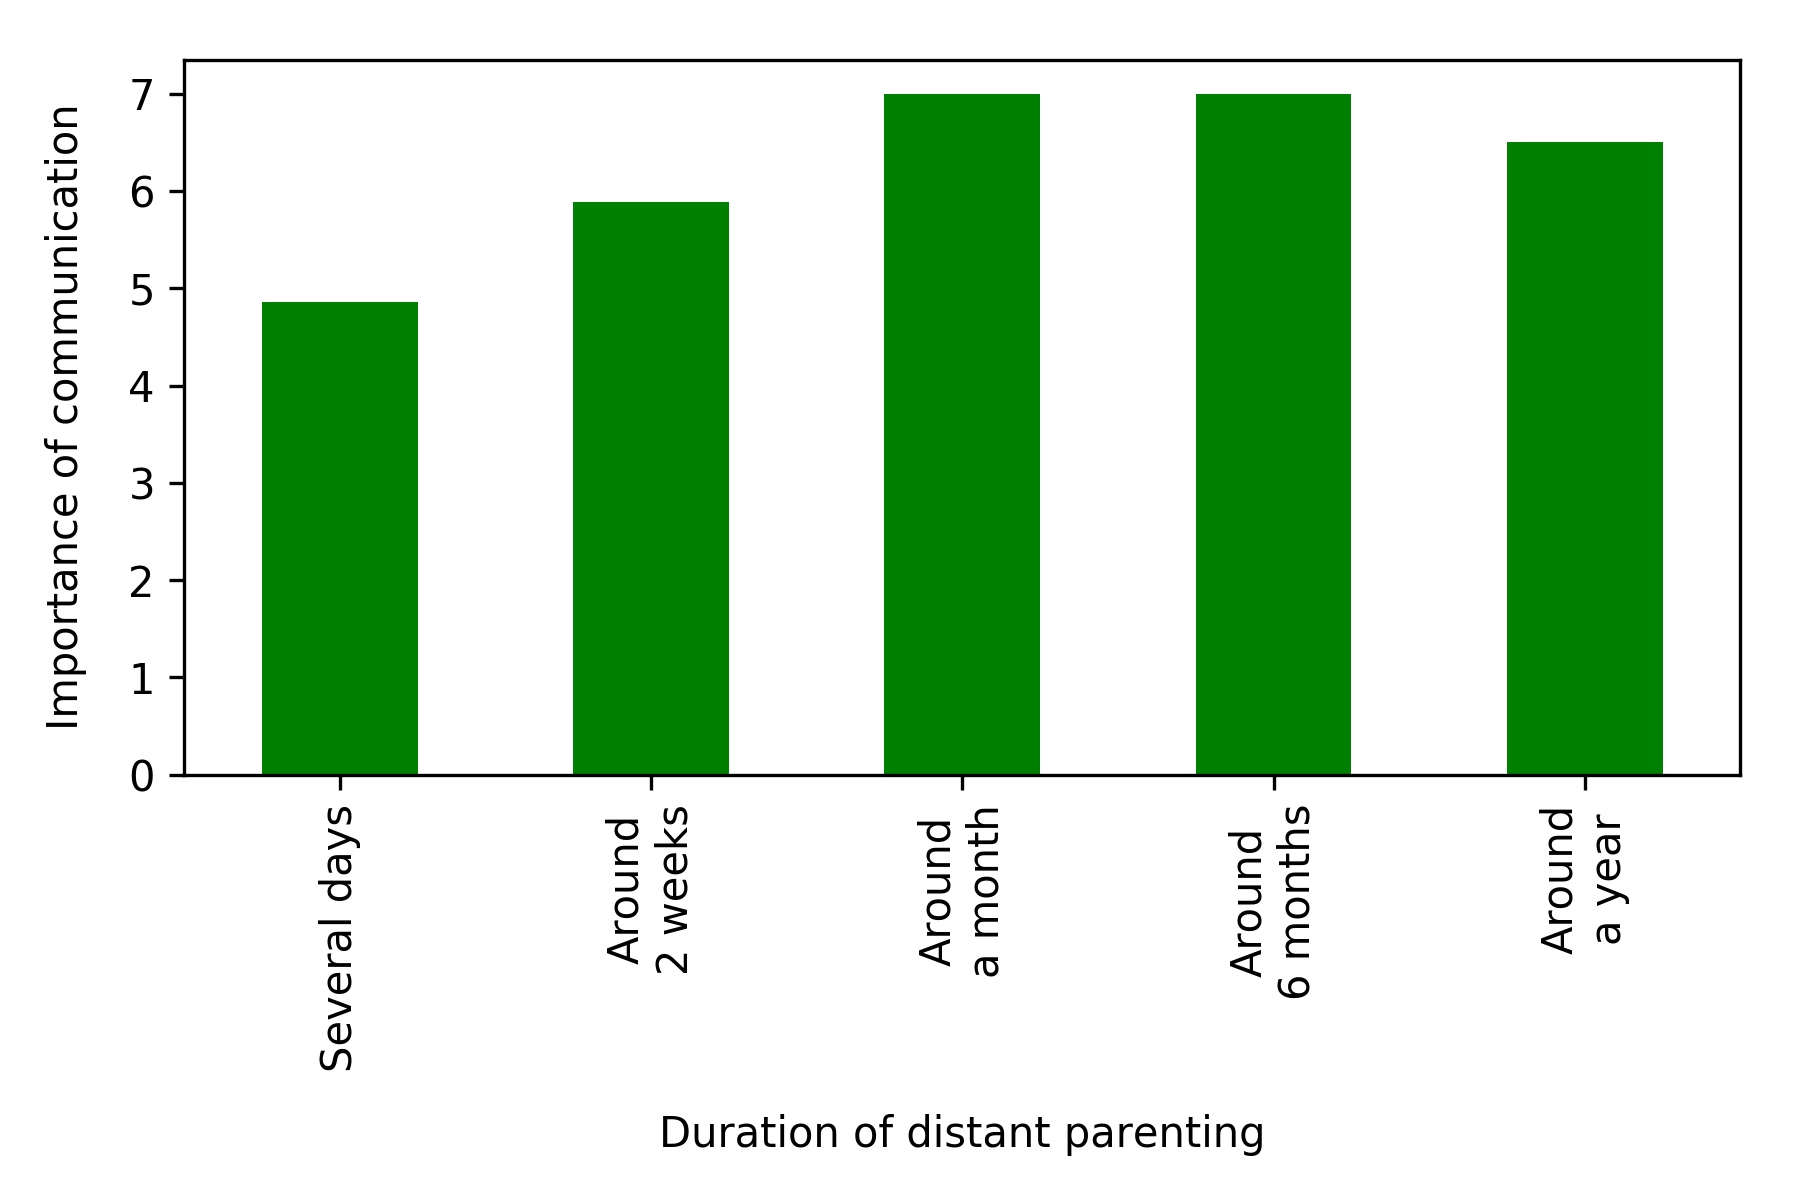
\includegraphics[scale=0.58]{plots/plot_5.png}
    \caption{Importance of communication from the parent point according to duration of distant-parenting experience}
    \label{fig:plot_5}
\end{figure}

\begin{figure}[h!]
    \centering
    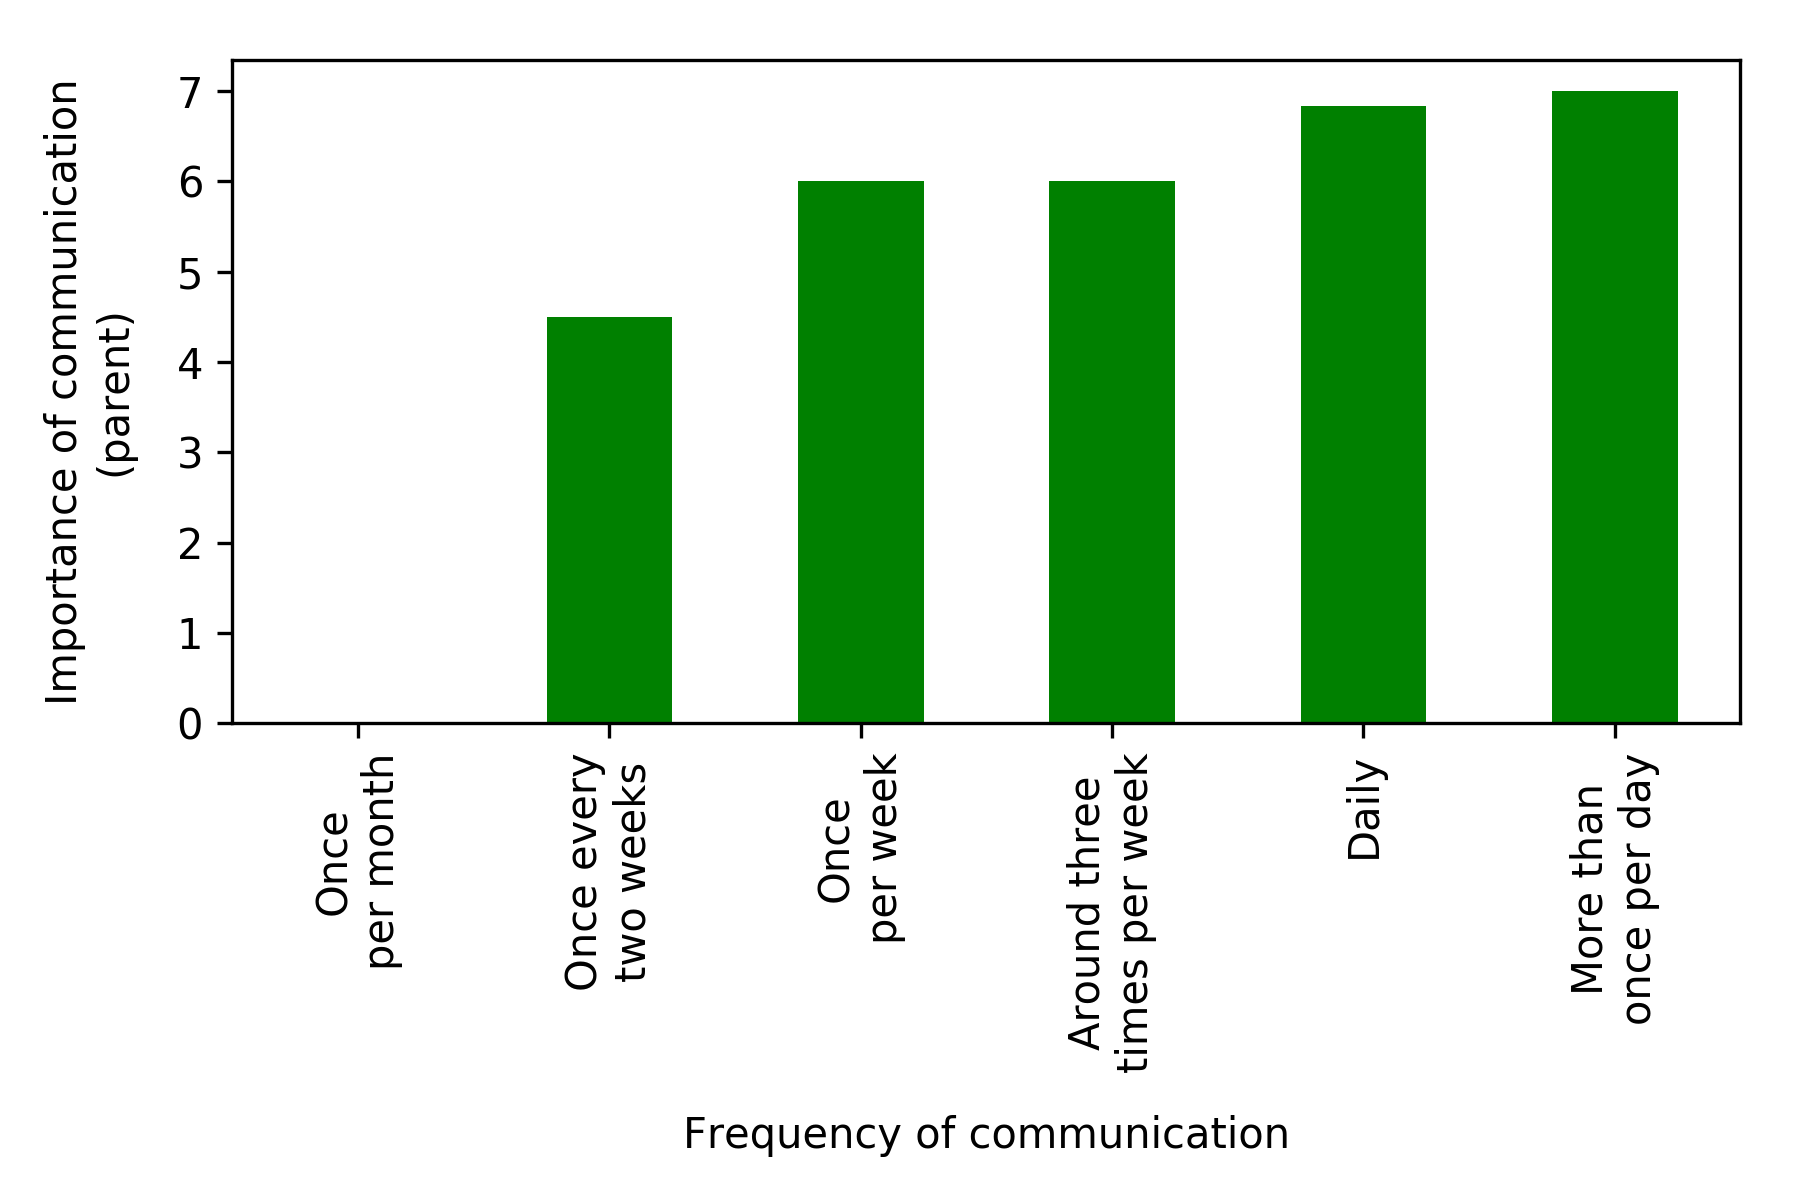
\includegraphics[scale=0.58]{plots/plot_8.png}
    \caption{Importance of communication from the parent point according to frequency of communication during distant-parenting experience}
    \label{fig:plot_8}
\end{figure}


\subsection{Interview protocol}
\label{appendix:interview_protocol}

The following interview protocol has been prepared for the research on “Communication Technologies for Left-Behind Children in Rural China”, in the scope of the “Global perspectives, local realities” SHS course. To continue our research on the Chinese field, by interviewing parents of left behind children, our assumptions could be tested and eventually further analyzed.

\vspace{4pt}
Please, fill in the missing informations as follows before starting the interview session:

Author: Matteo Yann Feo \& Simone Sanso

Session length: 40 minutes 

Participant Name: \hfill \_\_\_\_\_\_\_\_\_\_\_\_\_\_\_\_\_\_\_\_\_\_\_  $\leftarrow$ Fill in

Email: \hfill \_\_\_\_\_\_\_\_\_\_\_\_\_\_\_\_\_\_\_\_\_\_\_\_\_\_\_\_\_\_\_\_ $\leftarrow$ Fill in

Time/Date: \hfill \_\_\_\_\_\_\_\_\_\_\_\_\_\_\_\_\_\_\_\_\_\_\_\_\_\_\_\_ $\leftarrow$ Fill in

Location: \hfill \_\_\_\_\_\_\_\_\_\_\_\_\_\_\_\_\_\_\_\_\_\_\_\_\_\_\_\_\_ $\leftarrow$ Fill in

\vspace{6pt}
\subsubsection{Introduction \& Setup (5 mins)}

The session starts with a short introduction to what this interview is about, the context and the background for which it is being conducted. In the meantime, be sure that everything is setup correctly by double checking the following To-Do list:

\begin{todolist}
    \item Setup the recording tools and check if they work correctly.
    \item Prepare note-taking utilities, such as pen and paper.
    \item Verify the environment, being sure to have a relaxed location for the following 40 mins.
    \item In case a beverage is desired in the meantime, be sure to have it ready and available now.
    \item Be sure that your interviewed person has everything needed.
\end{todolist}

The introduction of the interview could be similar to the following one:

"Good morning and thank you for participating! I am Yann. I am studying at EPFL for a master degree in computer science. My main interest for this interview is to understand whether  a  technology  of  communication embedded in a smart toy could be helpful for parents distant from their children. During the interview, I will be having a conversation with you, asking questions that could help me to achieve my curiosity. In the meantime, my partner, will be assisting me by taking some notes. It is important to always remember that we are not evaluating you or your opinions in any way, there are no possible right and wrong answers that you could give. 
Here is how the session is going to proceed. Firstly, we'll break the ice by asking you a few general questions to know each other. We will record this interview, given your consent. We won't ever share this recording nor use it for anything else but pure support for this interview, so that I can go back and review things later to make sure we got everything right. Your name won't ever be linked to any result, so be relaxed and feel free to share your thoughts with us, without any troubles. Keep in mind that this is completely voluntary, the recording can be stopped whenever you want. Thus, if you don't like this idea, please let me know. 
How does all that sound to you? Do you have any questions at this point?"

\begin{todolist}
    \item Ask the interviewee to sign the written consent for recording purposes.
\end{todolist}

\vspace{2pt}
\subsubsection{Demographics \& Background (5 mins)}

This section will help us to create a background of the interviewee, while allowing him/her to start opening up to our questions. Use this session as a warming-up occasion to break the ice, while catching the first important features. Start to note down details on the interviewee, like gender, age, education level, marital status.

\begin{todolist}
    \item Tell us your name, and a little bit about yourself.
    \item Where do you come from?
    \item What is your occupation? Are you studying or working? In both cases, can you tell us something about it?
    \item Where are you currently living? Do you live with someone, or alone? 
\end{todolist}

\vspace{2pt}
\subsubsection{Main questions (20 mins)}

The following questions can be helpful to interpolate your impressions with the interviewee’s feelings and personal stories. Use them carefully as they might be intimidating for some people. Don’t forget to check for nonverbal behaviors, as they might be critical to have a complete idea of who you are interviewing, especially in this part. Note that the most important questions to be answered are marked with an asterisk (*).

\vspace{2pt}
(*) Pre-interview questions about their children :

\begin{todolist}
    \item How many children do you have?
    \item How old are they?
    \item What gender are they?
    \item Where do you they live?
    \item With who are they staying in your home village? (Lonely, with one of both parents, with grandparents or other relatives)
\end{todolist}

Main interview questions about the interviewed parent :

\begin{todolist}
    \item (*) How often and for how long do you come back home? 
    \item What is the main reason why you live far away from your children?
    \item How do you feel about this situation, not living with your children?
    \item Remember the last time you went back to your home village, how was the contact with your children? Was the meeting with your children as before you left them?
    \item During your childhood, have you ever experienced living far away from one of your parents? If yes, for how long? How did you live the situation? Could you tell us what was the main reason of your parent to out-migrate? How was the contact when meeting again with your parent? Could you communicate together, at that time, while being distant? (Check for non-verbal reactions while interviewee showcase personal experience)
    \item How common is your situation of distant parenting? Do you know any other persons in the same situation as you? How do they live it?
    \item (*) How would you define the importance of living with your children? In your case, is there a trade off between living with your children and having a job position? If yes, imagine that you could live in an ideal world, what would be the best solution? Would you rather work in your home village or be able to bring your children in town?
    \item (*) Do you own electronic devices? If yes, which ones? (Smartphone, computer, more…)
    \item (*) Do your children in your home village own electronic devices? If not, would they have the opportunity to use any? (Neighbourhood, school, etc.)
    \item (*) Do you use electronic devices to contact your children? If yes, how often? In general, are you calling your children when you have time? Or do they also get in touch with you, on their initiative?
    \item (*) From 0 to 7, how would you define the importance of communicating with your children? (0: insignificant, 4: neutral, 7: essential) (Check for non-verbal reactions while interviewee showcase personal experience)
\end{todolist}

\vspace{2pt}
\subsubsection{Interviewee's "show and tell" prototype (8 mins)}

This section is practical and allows us to showcase our project, related to the issue of distant parenting. In the context of CHIC (China Hardware Innovation Camp), a plush toy that encourages social interaction between parents and children, in a distant situation. It is a very resourceful moment, as it could bring additional and authentic feedback on a novel user scenario.

The explanation of the prototype could be similar to the following one:

"We have been working on this prototype. It is a plush toy that encourages social interaction, by having remotely turned on LEDs and sounds from a mobile application. Parents and children can therefore stay longer connected. Letting your children know when you think about them will help you stay 'toygether'\texttrademark."

Showcase the prototype and how it works with the mobile application.

\begin{todolist}
    \item What do you think about the idea?
    \item In your opinion, which are the positive and negative aspects?
    \item If you had the possibility to try this technology, would you be interested?
    \item What would you modify to improve it?
\end{todolist}

\vspace{2pt}
\subsubsection{Closing (2 mins)}

Thank the user at the end for participating to the session. Offer the possibility to ask any kind of question the interviewee might want to address you.  This is his/her time to wear the interviewer's shoes in your regards.

If the interviewee has no additional question, the interview is officially finished. Thank again your interviewee for the time and availability to participate to this session. Underline how useful his/her help has been for the project.
Turn off the recording tools only when you are completely sure that nothing will be added. It is important to not miss anything, so better have some extra recording to cut later.

Take some time to, directly after the end of the interview, write down some impressions you may have about the session. It is important to note down very early impressions about both verbal and physical languages, before they are forgotten. Those are the most authentic resources to get.




\subsection{List of contacts}
\label{appendix:contacts_list}
Below are listed all the contacts that have been reached, to spread as much as possible the survey.

\begin{itemize}
\item AFS programs for adolescents (15-18 years old): \\
Duration: 1 year \\
Kernstrasse 57, CH-8004 Zurich \\
Tel: +41 21 323 19 19 \\
Email: hello@afs.ch \\
https://www.afs.ch/fr/programmes-scolaires/ 

\vspace{4pt}
\item Canada-France exchange (16 years old): \\
Duration : 3 weeks \\
College of Jeanne d'Arc, 15 Rue du Chanoine Brun, 68100 Mulhouse, France \\
Tel: +33 3 89 45 36 31 \\
www.ejda.fr/ 

\vspace{4pt}
\item International exchange programs (14-18 years old): \\
Duration: 1 year \\
Rue Centrale 15, 1003 Lausanne \\
Tel: +41 800 822 811 \\
https://www.efswiss.ch/fr/highschool/ 

\vspace{4pt}
\item National observatory of the Erasmus + impact (1 year or 6 months): \\
Email: observatoire@agence-erasmus.fr \\
http://www.agence-erasmus.fr/page/observatoire/

\vspace{4pt}
\item Journal of international mobility:\\
Email: revue@agence-erasmus.fr \\
https://www.agence-erasmus.fr/page/JIM

\vspace{4pt}
\item Exchange program Brigitte Sauzay (14-17 years old): \\
Duration: 3 months in a host family in Germany and welcome 3 months in the family in France \\
https://www.ofaj.org/contact.html 

\vspace{4pt}
\item Internal exchanges and language stays in Switzerland (14-17 years old): \\
Duration: 1 year \\
College of Delémont, Avenue Station 7, 2800 Delémont \\
Tel: +41 32 421 00 70 \\
Email: info@coldel.org \\
http://www.college-delemont.ch/fr/Aide-aux-eleves/Echanges-et-sejours-linguistiques/Echanges-et-sejours-linguistiques.html \\
Cantonal manager of linguistic exchanges: \\
Patrice KAMBER, Pâquerettes 2, 2822 Courroux \\
- Prof: 032 435 65 92 / Private: 032 422 83 62 

\vspace{4pt}
\item Language Exchange and Mobility - DIP Geneva: \\
Catherine Fernandez Sonino: Head of Exchange \& Mobility DIP of the Cantonal Office for Language Exchange and Mobility \\
Chemin de l'Echo 5a, 1213 Onex \\
Email: catherine.fernandez@etat.ge.ch \\
Tel: +41 22 327 06 43, +41 79 175 56 46 \\
https://edu.ge.ch/site/elem/ 

\vspace{4pt}
\item Service of primary and secondary schools of Lausanne: \\
Place Chauderon 9, 5th floor, PO Box 5032, 1002 Lausanne \\
Tel: +41 21 315 64 11 - Fax: +41 21 315 60 04 \\
Email: seps@lausanne.ch \\
http://www.lausanne.ch/etablissements-scolaires/ 

\vspace{4pt}
\item Summer camp of Neuchatel:\\
Gisèle Nicaty \\
Quartier du Milieu 86, 2127 Les Bayards \\
Tel: +41 79 288 50 41, +41 32 866 17 29\\
Email: giroud.p-a@bluewin.ch\\
http://www.echanges-scolaires.com/index.php/fr/

\vspace{4pt}
\item Summer camp of the Grandes-Roches: \\
1348 le Brassus \\
Tel: +41 21 845 66 90 \\
Email: camps@asime.ch \\
http://www.grandesroches.ch/home 

\vspace{4pt}
\item Association of the Gros-de-Vaud Holiday Camp: \\
Mrs Florence Ethenoz \\
Chemin du Petit Record 60, 1040 Echallens \\
Tel: +41 21 881 10 76 \\
Email: info@colo-gros-de-vaud.ch \\
http://www.colo-gros-de-vaud.ch/clubdesk/www

\vspace{4pt}
\item Summer camp 4Fun: \\
Email: airfred@hotmail.com \\
http://4-fun.ch/ 

\vspace{4pt}
\item Summer camp CPV: \\
Swiss Village Street 14, PO Box 72, 1211 Geneva 8 \\
Tel: +41 22 809 49 79 \\
Email: info@camps.ch \\
http://www.camps.ch/fr/accueil 

\vspace{4pt}
\item Scouts of the Sacred Heart: \\
Jeanne Voruz \& Anne Thiébaud \\
Tel: +41 79 844 92 74 \& +41 79 284 50 38 \\
Email: cg@sacrescout.ch \\
http://www.sacrescout.ch/ 

\vspace{4pt}
\item Village Camps: \\
PO Box 1425, Rue de la Morache 14, 1260 Nyon 1 \\
Tel: +41 22 990 9400 \\
Email: camps@villagecamps.com \\
www.villagecamps.com

\vspace{4pt}
\item Alpadia Language Schools: \\
Grand-Rue 42, PO Box 1206, 1820 Montreux\\
Tel: +41 21 621 88 88\\
Email: info@alpadia.com\\
https://www.alpadia.com/fr/ 

\vspace{4pt}
\item Carol Panchaud Educom sàrl: \\
26 Route of Givrins, CH - 1276 Gingins\\
Tel: +41 22 776 69 15 \\
Email: carolpanchaud@educom.ch \\
http://educom.ch/fr

\vspace{4pt}
\item Caritas-Youth: \\
11, Jean-Violette Street, 1205 Geneva\\
Tel: +41 22 708 04 04\\
Email: info@caritas-jeunesse.ch\\
http://www.caritas-jeunesse.ch/

\vspace{4pt}
\item Holiday Camp St. Gervais: \\
CP 1337, 1211 Geneva 1\\
Tel: +41 78 896 71 84\\
Email: info@colonie-saint-gervais.ch\\
http://www.colonie-saint-gervais.ch/

\vspace{4pt}
\item Summer Camp of Ravoire - Camp Plein Soleil: \\
PO Box 87, CH-1920 Martigny 1\\
Email: info@camp-pleinsoleil.ch

\vspace{4pt}
\item Yverdon-les-Bains youth service and social cohesion: \\
Rue de Neuchâtel 2, 1400 Yverdon-les-Bains\\
Tel: +41 24 423 69 11\\
Email: vacances@yverdon-les-bains.ch\\
http://www.yverdon-les-bains.ch/prestations-deladministration/jeunesse-et-cohesion-sociale/enfanceetfamille/colonies-dete-et-dautomne/

\vspace{4pt}
\item fRilingue GmbH: \\
Stöckackerstrasse 93, 3018 Bern\\
Tel: +41 26 321 34 34 \\
Email: info@frilingue.com

\vspace{4pt}
\item Star Sports: \\
Path of Verger 2, PO Box 101, 1304 Cossonay-Ville\\
Tel: +41 79 356 44 61\\
Email: info@starsports.ch\\
http://www.starsports.ch/

\vspace{4pt}
\item Cap Loisirs Foundation: \\
34, Boulevard de Saint-Georges, 1205 Geneva\\
Tel: +41 22 731 86 00\\
Email: caploisirs@caploisirs.ch\\
http://www.caploisirs.ch/

\vspace{4pt}
\item SCE Holidays \& Events: \\
Rue de Lausanne 58, 1950 Sion\\
Tel: +41 79 693.33.64\\
Email: info@lescamps.ch\\
https://www.lescamps.ch/\\

\end{itemize}



% References of the Report
\thispagestyle{empty}
\vspace{1cm}
\begin{thebibliography}{9}
\addcontentsline{toc}{section}{References}

\bibitem{lab3-report} 
\textit{Lab 3.0 : Camera \& LCD conceptual design}. \\
CS-473 EPFL. Matteo Yann Feo \& Simone Aron Sanso. November 28th, 2017

\bibitem{lcd-controller} 
\textit{ILI9341 - a-Si TFT LCD Single Chip Driver 240RGBx320 Resolution and 262K color}. 
Rev. 1.11. ILI TECHNOLOGY CORP.

\bibitem{lcd-display} 
\textit{LT24 User Manual}. 
Altera. June 2015
 
\bibitem{avalon-interface} 
\textit{Avalon® Interface Specifications}.
MNL-AVABUSREF. Intel. May 2017.
 
\bibitem{fifo} 
\textit{Single- and Dual-Clock FIFO Megafunction}.
Rev. 4.0. Altera. May 2007.

\end{thebibliography}

\end{document}


% Appendix of the Report
\appendix

In the following appendix are presented the questions of the survey (... a list of figures and tables) to the reader.

\subsection{Questions of the survey}
\label{appendix:survey_questions}
In this section is shown how the participants were questioned towards the survey. Only the questions in English will be shown here, skipping the French translations.

\medskip \textit{Form about communication technologies :} \\
Realizing a research project about social sciences within EPFL University (Lausanne), we would like to understand the importance of communication between parents and children, when they are at a distance during a continuous period of time.

\vspace{4pt}
1. In what language would like to answer this form?

2. To contextualize, we seek either :

- parents of a child having spent a period of time away from the household,

- children, teenagers and young adults having spent a period of time away from their family.

After having read the description above, do you qualify yourself as a parent or a child?

\vspace{4pt}
\noindent - If "parent" was selected question 2: 

3.a. Are you the mother or the father?

4.a. Have you already been separated from your child for at least 3 days? (Exchange semester abroad, holidays, summer camp, boy-scout, etc.)

5.a. If there were more than one experience of distance parenting, please consider the earliest one of them through the rest of the form (when you were the youngest). What is the reason why your child was distant from you? 

6.a. For how long have you been distant from your child?

7.a. How old was your child at that time?

8.a. What is your child's gender?

9.a. How often did you use a communication technology with your distant child? (Text messages, phone calls, video chat, etc.)

10.a. What kind of information did you seek from communicating with your distant child?

11.a. How would you define the importance of being able to communicate with your distant child?

\vspace{4pt}
\noindent - If "child" was selected question 2: 

3.b. Have you already been separated from your family for at least 3 days? (Exchange semester abroad, holidays, summer camp, boy-scout, etc.)

3.b. If there were more than one experience of separation from your family, please consider the earliest one of them through the rest of the form (when you were the youngest). What is the reason why you were distant from your family? 

4.b. For how long have you been away?

5.b. How old were you at that time?

6.b. What is your gender?

7.b. How often did you use a communication technology with your family? (Text messages, phone calls, video chat, etc.)

8.b. What kind of information did you seek from communicating with your family?

9.b. How would you define the importance of being able to communicate with your family?


\subsection{Additional plots of the results}
\label{appendix:additional-plots}

The following plots have been computed for the analysis of the data collected via the survey on distant-parenting. This appendix contains a set of plots that didn't need particular attention during the discussion, but can still be source of investigation.

\begin{figure}[h!]
    \centering
    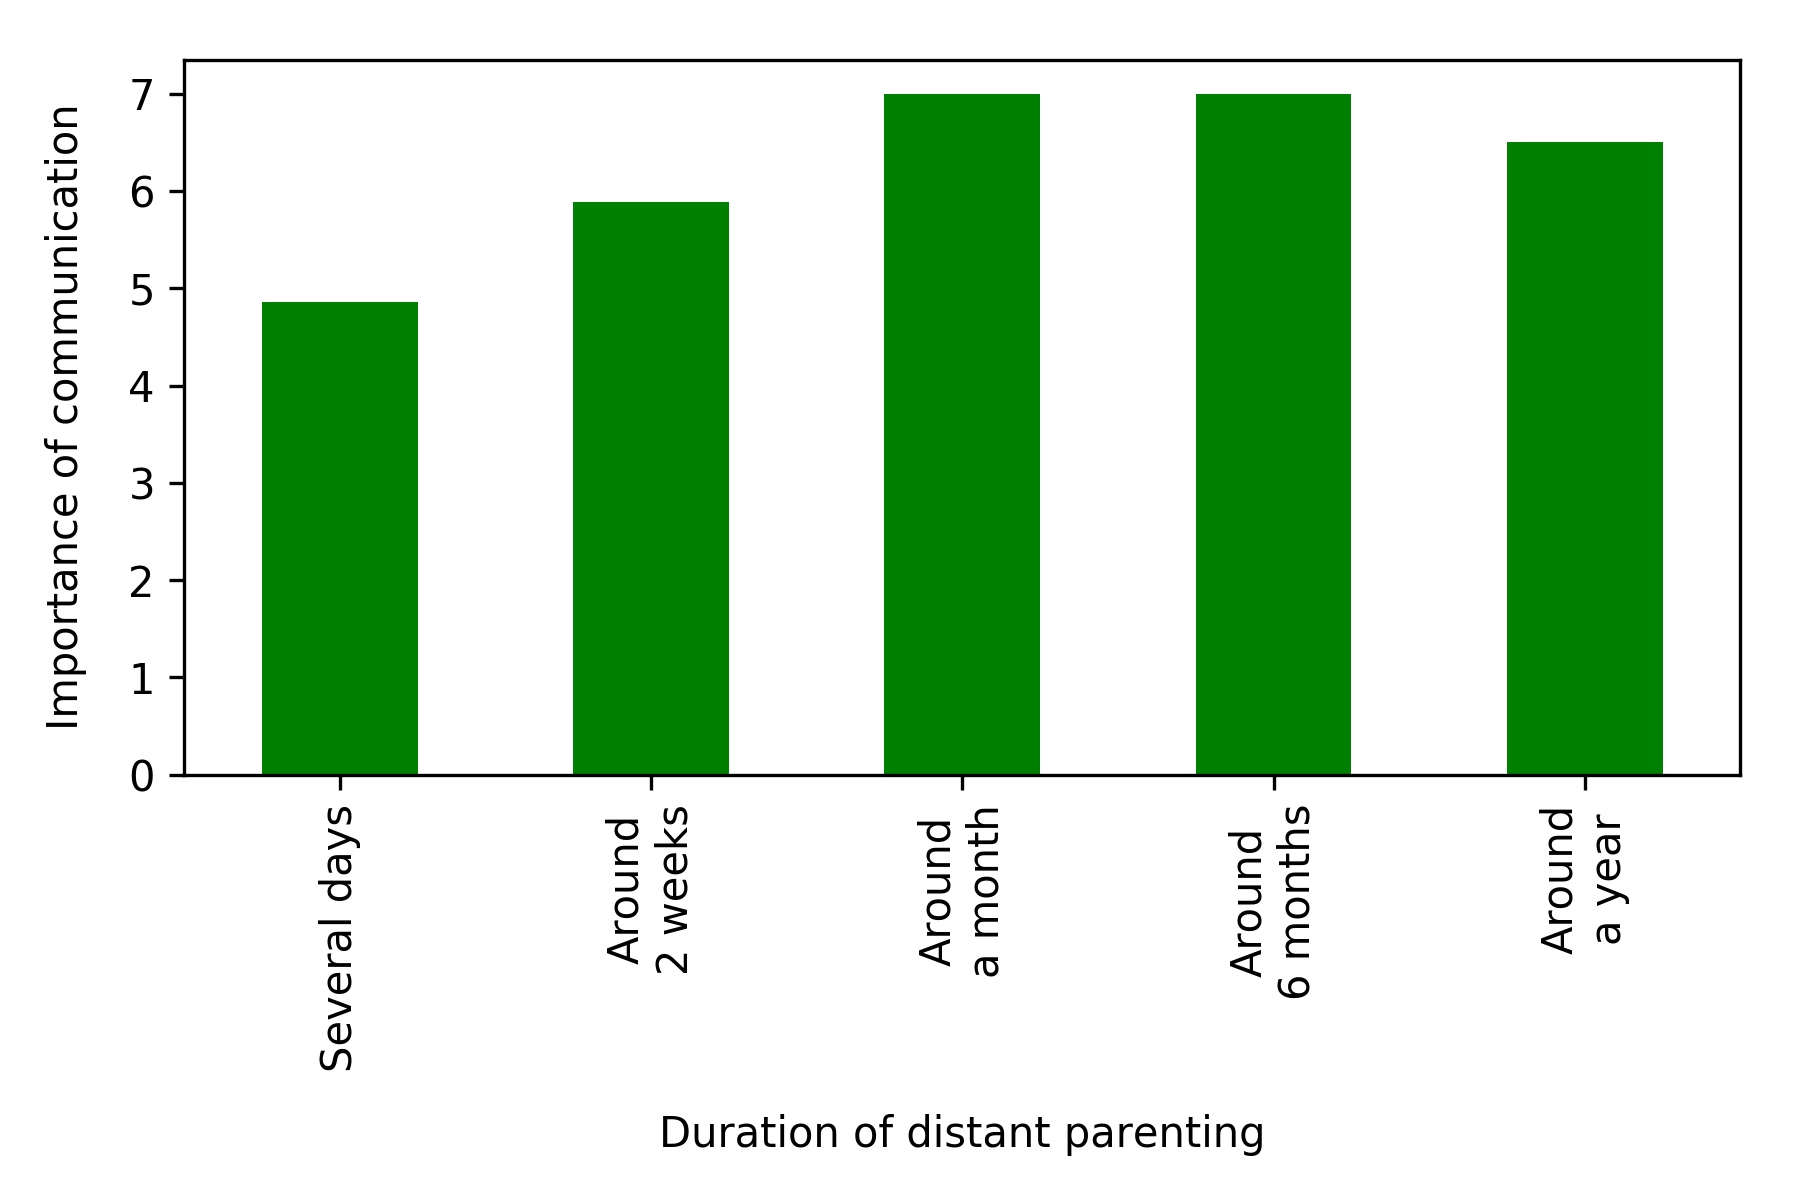
\includegraphics[scale=0.58]{plots/plot_5.png}
    \caption{Importance of communication from the parent point according to duration of distant-parenting experience}
    \label{fig:plot_5}
\end{figure}

\begin{figure}[h!]
    \centering
    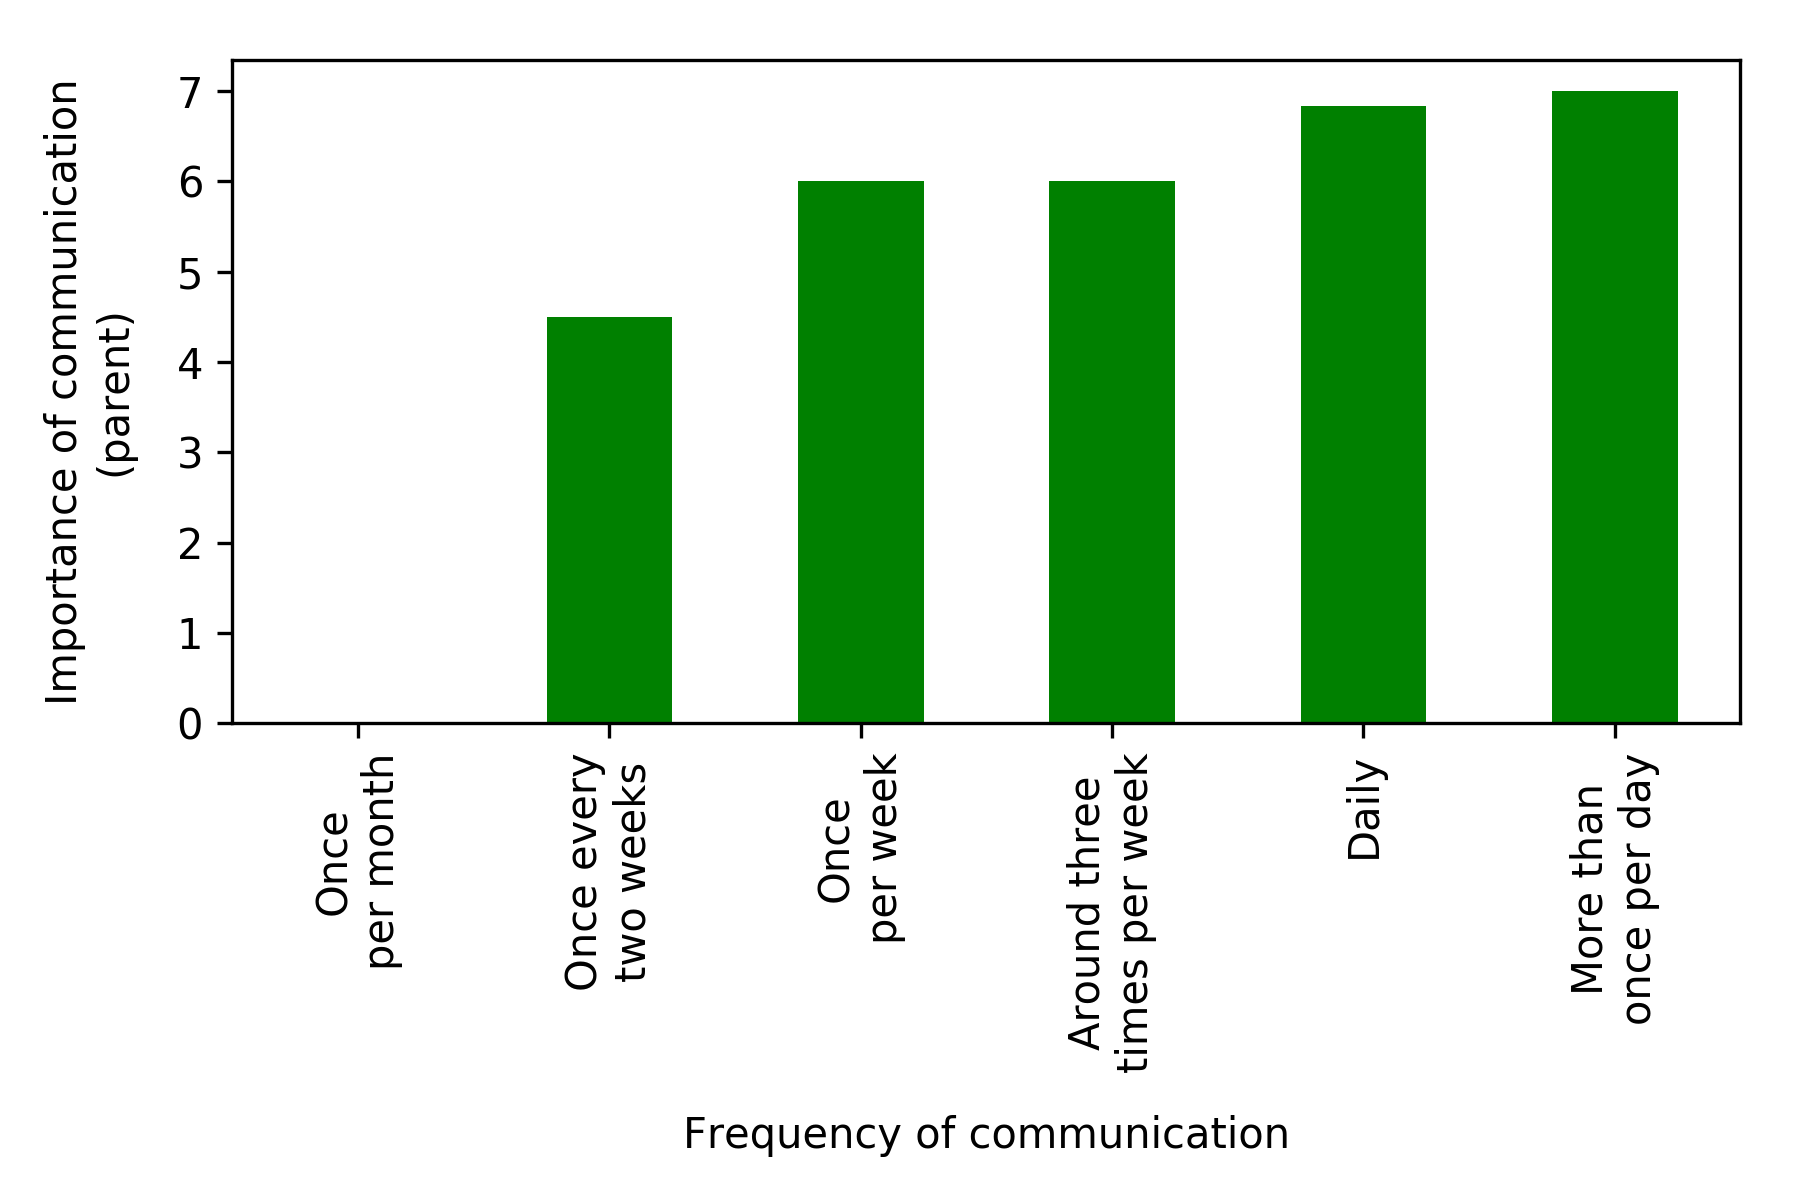
\includegraphics[scale=0.58]{plots/plot_8.png}
    \caption{Importance of communication from the parent point according to frequency of communication during distant-parenting experience}
    \label{fig:plot_8}
\end{figure}


\subsection{Interview protocol}
\label{appendix:interview_protocol}

The following interview protocol has been prepared for the research on “Communication Technologies for Left-Behind Children in Rural China”, in the scope of the “Global perspectives, local realities” SHS course. To continue our research on the Chinese field, by interviewing parents of left behind children, our assumptions could be tested and eventually further analyzed.

\vspace{4pt}
Please, fill in the missing informations as follows before starting the interview session:

Author: Matteo Yann Feo \& Simone Sanso

Session length: 40 minutes 

Participant Name: \hfill \_\_\_\_\_\_\_\_\_\_\_\_\_\_\_\_\_\_\_\_\_\_\_  $\leftarrow$ Fill in

Email: \hfill \_\_\_\_\_\_\_\_\_\_\_\_\_\_\_\_\_\_\_\_\_\_\_\_\_\_\_\_\_\_\_\_ $\leftarrow$ Fill in

Time/Date: \hfill \_\_\_\_\_\_\_\_\_\_\_\_\_\_\_\_\_\_\_\_\_\_\_\_\_\_\_\_ $\leftarrow$ Fill in

Location: \hfill \_\_\_\_\_\_\_\_\_\_\_\_\_\_\_\_\_\_\_\_\_\_\_\_\_\_\_\_\_ $\leftarrow$ Fill in

\vspace{6pt}
\subsubsection{Introduction \& Setup (5 mins)}

The session starts with a short introduction to what this interview is about, the context and the background for which it is being conducted. In the meantime, be sure that everything is setup correctly by double checking the following To-Do list:

\begin{todolist}
    \item Setup the recording tools and check if they work correctly.
    \item Prepare note-taking utilities, such as pen and paper.
    \item Verify the environment, being sure to have a relaxed location for the following 40 mins.
    \item In case a beverage is desired in the meantime, be sure to have it ready and available now.
    \item Be sure that your interviewed person has everything needed.
\end{todolist}

The introduction of the interview could be similar to the following one:

"Good morning and thank you for participating! I am Yann. I am studying at EPFL for a master degree in computer science. My main interest for this interview is to understand whether  a  technology  of  communication embedded in a smart toy could be helpful for parents distant from their children. During the interview, I will be having a conversation with you, asking questions that could help me to achieve my curiosity. In the meantime, my partner, will be assisting me by taking some notes. It is important to always remember that we are not evaluating you or your opinions in any way, there are no possible right and wrong answers that you could give. 
Here is how the session is going to proceed. Firstly, we'll break the ice by asking you a few general questions to know each other. We will record this interview, given your consent. We won't ever share this recording nor use it for anything else but pure support for this interview, so that I can go back and review things later to make sure we got everything right. Your name won't ever be linked to any result, so be relaxed and feel free to share your thoughts with us, without any troubles. Keep in mind that this is completely voluntary, the recording can be stopped whenever you want. Thus, if you don't like this idea, please let me know. 
How does all that sound to you? Do you have any questions at this point?"

\begin{todolist}
    \item Ask the interviewee to sign the written consent for recording purposes.
\end{todolist}

\vspace{2pt}
\subsubsection{Demographics \& Background (5 mins)}

This section will help us to create a background of the interviewee, while allowing him/her to start opening up to our questions. Use this session as a warming-up occasion to break the ice, while catching the first important features. Start to note down details on the interviewee, like gender, age, education level, marital status.

\begin{todolist}
    \item Tell us your name, and a little bit about yourself.
    \item Where do you come from?
    \item What is your occupation? Are you studying or working? In both cases, can you tell us something about it?
    \item Where are you currently living? Do you live with someone, or alone? 
\end{todolist}

\vspace{2pt}
\subsubsection{Main questions (20 mins)}

The following questions can be helpful to interpolate your impressions with the interviewee’s feelings and personal stories. Use them carefully as they might be intimidating for some people. Don’t forget to check for nonverbal behaviors, as they might be critical to have a complete idea of who you are interviewing, especially in this part. Note that the most important questions to be answered are marked with an asterisk (*).

\vspace{2pt}
(*) Pre-interview questions about their children :

\begin{todolist}
    \item How many children do you have?
    \item How old are they?
    \item What gender are they?
    \item Where do you they live?
    \item With who are they staying in your home village? (Lonely, with one of both parents, with grandparents or other relatives)
\end{todolist}

Main interview questions about the interviewed parent :

\begin{todolist}
    \item (*) How often and for how long do you come back home? 
    \item What is the main reason why you live far away from your children?
    \item How do you feel about this situation, not living with your children?
    \item Remember the last time you went back to your home village, how was the contact with your children? Was the meeting with your children as before you left them?
    \item During your childhood, have you ever experienced living far away from one of your parents? If yes, for how long? How did you live the situation? Could you tell us what was the main reason of your parent to out-migrate? How was the contact when meeting again with your parent? Could you communicate together, at that time, while being distant? (Check for non-verbal reactions while interviewee showcase personal experience)
    \item How common is your situation of distant parenting? Do you know any other persons in the same situation as you? How do they live it?
    \item (*) How would you define the importance of living with your children? In your case, is there a trade off between living with your children and having a job position? If yes, imagine that you could live in an ideal world, what would be the best solution? Would you rather work in your home village or be able to bring your children in town?
    \item (*) Do you own electronic devices? If yes, which ones? (Smartphone, computer, more…)
    \item (*) Do your children in your home village own electronic devices? If not, would they have the opportunity to use any? (Neighbourhood, school, etc.)
    \item (*) Do you use electronic devices to contact your children? If yes, how often? In general, are you calling your children when you have time? Or do they also get in touch with you, on their initiative?
    \item (*) From 0 to 7, how would you define the importance of communicating with your children? (0: insignificant, 4: neutral, 7: essential) (Check for non-verbal reactions while interviewee showcase personal experience)
\end{todolist}

\vspace{2pt}
\subsubsection{Interviewee's "show and tell" prototype (8 mins)}

This section is practical and allows us to showcase our project, related to the issue of distant parenting. In the context of CHIC (China Hardware Innovation Camp), a plush toy that encourages social interaction between parents and children, in a distant situation. It is a very resourceful moment, as it could bring additional and authentic feedback on a novel user scenario.

The explanation of the prototype could be similar to the following one:

"We have been working on this prototype. It is a plush toy that encourages social interaction, by having remotely turned on LEDs and sounds from a mobile application. Parents and children can therefore stay longer connected. Letting your children know when you think about them will help you stay 'toygether'\texttrademark."

Showcase the prototype and how it works with the mobile application.

\begin{todolist}
    \item What do you think about the idea?
    \item In your opinion, which are the positive and negative aspects?
    \item If you had the possibility to try this technology, would you be interested?
    \item What would you modify to improve it?
\end{todolist}

\vspace{2pt}
\subsubsection{Closing (2 mins)}

Thank the user at the end for participating to the session. Offer the possibility to ask any kind of question the interviewee might want to address you.  This is his/her time to wear the interviewer's shoes in your regards.

If the interviewee has no additional question, the interview is officially finished. Thank again your interviewee for the time and availability to participate to this session. Underline how useful his/her help has been for the project.
Turn off the recording tools only when you are completely sure that nothing will be added. It is important to not miss anything, so better have some extra recording to cut later.

Take some time to, directly after the end of the interview, write down some impressions you may have about the session. It is important to note down very early impressions about both verbal and physical languages, before they are forgotten. Those are the most authentic resources to get.




\subsection{List of contacts}
\label{appendix:contacts_list}
Below are listed all the contacts that have been reached, to spread as much as possible the survey.

\begin{itemize}
\item AFS programs for adolescents (15-18 years old): \\
Duration: 1 year \\
Kernstrasse 57, CH-8004 Zurich \\
Tel: +41 21 323 19 19 \\
Email: hello@afs.ch \\
https://www.afs.ch/fr/programmes-scolaires/ 

\vspace{4pt}
\item Canada-France exchange (16 years old): \\
Duration : 3 weeks \\
College of Jeanne d'Arc, 15 Rue du Chanoine Brun, 68100 Mulhouse, France \\
Tel: +33 3 89 45 36 31 \\
www.ejda.fr/ 

\vspace{4pt}
\item International exchange programs (14-18 years old): \\
Duration: 1 year \\
Rue Centrale 15, 1003 Lausanne \\
Tel: +41 800 822 811 \\
https://www.efswiss.ch/fr/highschool/ 

\vspace{4pt}
\item National observatory of the Erasmus + impact (1 year or 6 months): \\
Email: observatoire@agence-erasmus.fr \\
http://www.agence-erasmus.fr/page/observatoire/

\vspace{4pt}
\item Journal of international mobility:\\
Email: revue@agence-erasmus.fr \\
https://www.agence-erasmus.fr/page/JIM

\vspace{4pt}
\item Exchange program Brigitte Sauzay (14-17 years old): \\
Duration: 3 months in a host family in Germany and welcome 3 months in the family in France \\
https://www.ofaj.org/contact.html 

\vspace{4pt}
\item Internal exchanges and language stays in Switzerland (14-17 years old): \\
Duration: 1 year \\
College of Delémont, Avenue Station 7, 2800 Delémont \\
Tel: +41 32 421 00 70 \\
Email: info@coldel.org \\
http://www.college-delemont.ch/fr/Aide-aux-eleves/Echanges-et-sejours-linguistiques/Echanges-et-sejours-linguistiques.html \\
Cantonal manager of linguistic exchanges: \\
Patrice KAMBER, Pâquerettes 2, 2822 Courroux \\
- Prof: 032 435 65 92 / Private: 032 422 83 62 

\vspace{4pt}
\item Language Exchange and Mobility - DIP Geneva: \\
Catherine Fernandez Sonino: Head of Exchange \& Mobility DIP of the Cantonal Office for Language Exchange and Mobility \\
Chemin de l'Echo 5a, 1213 Onex \\
Email: catherine.fernandez@etat.ge.ch \\
Tel: +41 22 327 06 43, +41 79 175 56 46 \\
https://edu.ge.ch/site/elem/ 

\vspace{4pt}
\item Service of primary and secondary schools of Lausanne: \\
Place Chauderon 9, 5th floor, PO Box 5032, 1002 Lausanne \\
Tel: +41 21 315 64 11 - Fax: +41 21 315 60 04 \\
Email: seps@lausanne.ch \\
http://www.lausanne.ch/etablissements-scolaires/ 

\vspace{4pt}
\item Summer camp of Neuchatel:\\
Gisèle Nicaty \\
Quartier du Milieu 86, 2127 Les Bayards \\
Tel: +41 79 288 50 41, +41 32 866 17 29\\
Email: giroud.p-a@bluewin.ch\\
http://www.echanges-scolaires.com/index.php/fr/

\vspace{4pt}
\item Summer camp of the Grandes-Roches: \\
1348 le Brassus \\
Tel: +41 21 845 66 90 \\
Email: camps@asime.ch \\
http://www.grandesroches.ch/home 

\vspace{4pt}
\item Association of the Gros-de-Vaud Holiday Camp: \\
Mrs Florence Ethenoz \\
Chemin du Petit Record 60, 1040 Echallens \\
Tel: +41 21 881 10 76 \\
Email: info@colo-gros-de-vaud.ch \\
http://www.colo-gros-de-vaud.ch/clubdesk/www

\vspace{4pt}
\item Summer camp 4Fun: \\
Email: airfred@hotmail.com \\
http://4-fun.ch/ 

\vspace{4pt}
\item Summer camp CPV: \\
Swiss Village Street 14, PO Box 72, 1211 Geneva 8 \\
Tel: +41 22 809 49 79 \\
Email: info@camps.ch \\
http://www.camps.ch/fr/accueil 

\vspace{4pt}
\item Scouts of the Sacred Heart: \\
Jeanne Voruz \& Anne Thiébaud \\
Tel: +41 79 844 92 74 \& +41 79 284 50 38 \\
Email: cg@sacrescout.ch \\
http://www.sacrescout.ch/ 

\vspace{4pt}
\item Village Camps: \\
PO Box 1425, Rue de la Morache 14, 1260 Nyon 1 \\
Tel: +41 22 990 9400 \\
Email: camps@villagecamps.com \\
www.villagecamps.com

\vspace{4pt}
\item Alpadia Language Schools: \\
Grand-Rue 42, PO Box 1206, 1820 Montreux\\
Tel: +41 21 621 88 88\\
Email: info@alpadia.com\\
https://www.alpadia.com/fr/ 

\vspace{4pt}
\item Carol Panchaud Educom sàrl: \\
26 Route of Givrins, CH - 1276 Gingins\\
Tel: +41 22 776 69 15 \\
Email: carolpanchaud@educom.ch \\
http://educom.ch/fr

\vspace{4pt}
\item Caritas-Youth: \\
11, Jean-Violette Street, 1205 Geneva\\
Tel: +41 22 708 04 04\\
Email: info@caritas-jeunesse.ch\\
http://www.caritas-jeunesse.ch/

\vspace{4pt}
\item Holiday Camp St. Gervais: \\
CP 1337, 1211 Geneva 1\\
Tel: +41 78 896 71 84\\
Email: info@colonie-saint-gervais.ch\\
http://www.colonie-saint-gervais.ch/

\vspace{4pt}
\item Summer Camp of Ravoire - Camp Plein Soleil: \\
PO Box 87, CH-1920 Martigny 1\\
Email: info@camp-pleinsoleil.ch

\vspace{4pt}
\item Yverdon-les-Bains youth service and social cohesion: \\
Rue de Neuchâtel 2, 1400 Yverdon-les-Bains\\
Tel: +41 24 423 69 11\\
Email: vacances@yverdon-les-bains.ch\\
http://www.yverdon-les-bains.ch/prestations-deladministration/jeunesse-et-cohesion-sociale/enfanceetfamille/colonies-dete-et-dautomne/

\vspace{4pt}
\item fRilingue GmbH: \\
Stöckackerstrasse 93, 3018 Bern\\
Tel: +41 26 321 34 34 \\
Email: info@frilingue.com

\vspace{4pt}
\item Star Sports: \\
Path of Verger 2, PO Box 101, 1304 Cossonay-Ville\\
Tel: +41 79 356 44 61\\
Email: info@starsports.ch\\
http://www.starsports.ch/

\vspace{4pt}
\item Cap Loisirs Foundation: \\
34, Boulevard de Saint-Georges, 1205 Geneva\\
Tel: +41 22 731 86 00\\
Email: caploisirs@caploisirs.ch\\
http://www.caploisirs.ch/

\vspace{4pt}
\item SCE Holidays \& Events: \\
Rue de Lausanne 58, 1950 Sion\\
Tel: +41 79 693.33.64\\
Email: info@lescamps.ch\\
https://www.lescamps.ch/\\

\end{itemize}



% References of the Report
\thispagestyle{empty}
\vspace{1cm}
\begin{thebibliography}{9}
\addcontentsline{toc}{section}{References}

\bibitem{lab3-report} 
\textit{Lab 3.0 : Camera \& LCD conceptual design}. \\
CS-473 EPFL. Matteo Yann Feo \& Simone Aron Sanso. November 28th, 2017

\bibitem{lcd-controller} 
\textit{ILI9341 - a-Si TFT LCD Single Chip Driver 240RGBx320 Resolution and 262K color}. 
Rev. 1.11. ILI TECHNOLOGY CORP.

\bibitem{lcd-display} 
\textit{LT24 User Manual}. 
Altera. June 2015
 
\bibitem{avalon-interface} 
\textit{Avalon® Interface Specifications}.
MNL-AVABUSREF. Intel. May 2017.
 
\bibitem{fifo} 
\textit{Single- and Dual-Clock FIFO Megafunction}.
Rev. 4.0. Altera. May 2007.

\end{thebibliography}

\end{document}


\documentclass[a4paper,12pt]{article}

%% Layout
\usepackage[utf8]{inputenc}
\usepackage{palatino}
\usepackage[T1]{fontenc}
\usepackage[8pt]{extsizes}

\usepackage{geometry}
\geometry{
    a4paper,
    total={170mm,257mm},
    left=30mm,
    right=30mm,
    top=30mm,
    bottom=30mm,
 } 

%% Useful packages
\usepackage{amsmath}
\usepackage{amssymb}
\usepackage{mathtools}
\usepackage{microtype}

\usepackage[usenames, dvipsnames]{xcolor}
\usepackage{graphicx}
\usepackage{wrapfig}
\usepackage{subfig}
\usepackage{tabularx}
\usepackage{float}
\usepackage{caption}
\usepackage{multirow}
\usepackage{color, colortbl}
\usepackage{enumerate}

\usepackage{hyperref}
\usepackage{url}

\usepackage[english]{babel}
\usepackage{units}

\usepackage{textcomp}
\usepackage{titling}
\usepackage{blindtext}
\usepackage{listings}

\usepackage{braket}
\usepackage{rotating}

%\setlength{\droptitle}{-4em}     % Eliminate the default vertical space
%\addtolength{\droptitle}{-4pt}

\title{
    \centering
	
\includegraphics[width=0.5\textwidth]{images/Logo_EPFL.png}
    \\[1cm]
	\Huge China Hardware Innovation Camp\\[1cm]
    \huge Semester project report\\
    \rule{3.5cm}{0.9pt}\\[0.5cm]
    \huge HUM - 498 \vfill
    \normalsize
}

\author{
    \textbf{Laboratory group:}\\\\
    Chloe Dickson - \texttt{\href{mailto:chloe.dickson@epfl.ch}{simone.sanso@epfl.ch}} \\
    Matteo Yann Feo -    \texttt{\href{mailto:matteo.feo@epfl.ch}{matteo.feo@epfl.ch}} \\
    Simone Aron Sanso - \texttt{\href{mailto:simone.sanso@epfl.ch}{simone.sanso@epfl.ch}} \\\\
}

\date{\vfill \today}

\lstdefinestyle{Python}{
  language=Python,                % choose the language of the code
  numbers=left,                   % where to put the line-numbers
  stepnumber=1,                   % the step between two line-numbers.        
  numbersep=5pt,                  % how far the line-numbers are from the code
  backgroundcolor=\color{white},  % choose the background color. You must add \usepackage{color}
  showspaces=false,               % show spaces adding particular underscores
  showstringspaces=false,         % underline spaces within strings
  showtabs=false,                 % show tabs within strings adding particular underscores
  tabsize=2,                      % sets default tabsize to 2 spaces
  captionpos=b,                   % sets the caption-position to bottom
  breaklines=true,                % sets automatic line breaking
  breakatwhitespace=true,         % sets if automatic breaks should only happen at whitespace
  frame=single, 
  basicstyle=\ttfamily,
  keywordstyle=\color{Green}\bfseries,
  stringstyle=\color{red}\ttfamily,
  commentstyle=\color{OliveGreen}\ttfamily,
  %morecomment=[l][\color{magenta}]{\#}
}


\begin{document}
\maketitle
\thispagestyle{empty}

\newpage
\thispagestyle{empty}
\setcounter{page}{0}

\tableofcontents

\documentclass[a4paper,12pt]{article}

%% Layout
\usepackage[utf8]{inputenc}
\usepackage{palatino}
\usepackage[T1]{fontenc}
\usepackage[8pt]{extsizes}

\usepackage{geometry}
\geometry{
    a4paper,
    total={170mm,257mm},
    left=30mm,
    right=30mm,
    top=30mm,
    bottom=30mm,
 } 

%% Useful packages
\usepackage{amsmath}
\usepackage{amssymb}
\usepackage{mathtools}
\usepackage{microtype}

\usepackage[usenames, dvipsnames]{xcolor}
\usepackage{graphicx}
\usepackage{wrapfig}
\usepackage{subfig}
\usepackage{tabularx}
\usepackage{float}
\usepackage{caption}
\usepackage{multirow}
\usepackage{color, colortbl}
\usepackage{enumerate}

\usepackage{hyperref}
\usepackage{url}

\usepackage[english]{babel}
\usepackage{units}

\usepackage{textcomp}
\usepackage{titling}
\usepackage{blindtext}
\usepackage{listings}

\usepackage{braket}
\usepackage{rotating}

%\setlength{\droptitle}{-4em}     % Eliminate the default vertical space
%\addtolength{\droptitle}{-4pt}

\title{
    \centering
	
\includegraphics[width=0.5\textwidth]{images/Logo_EPFL.png}
    \\[1cm]
	\Huge China Hardware Innovation Camp\\[1cm]
    \huge Semester project report\\
    \rule{3.5cm}{0.9pt}\\[0.5cm]
    \huge HUM - 498 \vfill
    \normalsize
}

\author{
    \textbf{Laboratory group:}\\\\
    Chloe Dickson - \texttt{\href{mailto:chloe.dickson@epfl.ch}{simone.sanso@epfl.ch}} \\
    Matteo Yann Feo -    \texttt{\href{mailto:matteo.feo@epfl.ch}{matteo.feo@epfl.ch}} \\
    Simone Aron Sanso - \texttt{\href{mailto:simone.sanso@epfl.ch}{simone.sanso@epfl.ch}} \\\\
}

\date{\vfill \today}

\lstdefinestyle{Python}{
  language=Python,                % choose the language of the code
  numbers=left,                   % where to put the line-numbers
  stepnumber=1,                   % the step between two line-numbers.        
  numbersep=5pt,                  % how far the line-numbers are from the code
  backgroundcolor=\color{white},  % choose the background color. You must add \usepackage{color}
  showspaces=false,               % show spaces adding particular underscores
  showstringspaces=false,         % underline spaces within strings
  showtabs=false,                 % show tabs within strings adding particular underscores
  tabsize=2,                      % sets default tabsize to 2 spaces
  captionpos=b,                   % sets the caption-position to bottom
  breaklines=true,                % sets automatic line breaking
  breakatwhitespace=true,         % sets if automatic breaks should only happen at whitespace
  frame=single, 
  basicstyle=\ttfamily,
  keywordstyle=\color{Green}\bfseries,
  stringstyle=\color{red}\ttfamily,
  commentstyle=\color{OliveGreen}\ttfamily,
  %morecomment=[l][\color{magenta}]{\#}
}


\begin{document}
\maketitle
\thispagestyle{empty}

\newpage
\thispagestyle{empty}
\setcounter{page}{0}

\tableofcontents

\documentclass[a4paper,12pt]{article}

%% Layout
\usepackage[utf8]{inputenc}
\usepackage{palatino}
\usepackage[T1]{fontenc}
\usepackage[8pt]{extsizes}

\usepackage{geometry}
\geometry{
    a4paper,
    total={170mm,257mm},
    left=30mm,
    right=30mm,
    top=30mm,
    bottom=30mm,
 } 

%% Useful packages
\usepackage{amsmath}
\usepackage{amssymb}
\usepackage{mathtools}
\usepackage{microtype}

\usepackage[usenames, dvipsnames]{xcolor}
\usepackage{graphicx}
\usepackage{wrapfig}
\usepackage{subfig}
\usepackage{tabularx}
\usepackage{float}
\usepackage{caption}
\usepackage{multirow}
\usepackage{color, colortbl}
\usepackage{enumerate}

\usepackage{hyperref}
\usepackage{url}

\usepackage[english]{babel}
\usepackage{units}

\usepackage{textcomp}
\usepackage{titling}
\usepackage{blindtext}
\usepackage{listings}

\usepackage{braket}
\usepackage{rotating}

%\setlength{\droptitle}{-4em}     % Eliminate the default vertical space
%\addtolength{\droptitle}{-4pt}

\title{
    \centering
	
\includegraphics[width=0.5\textwidth]{images/Logo_EPFL.png}
    \\[1cm]
	\Huge China Hardware Innovation Camp\\[1cm]
    \huge Semester project report\\
    \rule{3.5cm}{0.9pt}\\[0.5cm]
    \huge HUM - 498 \vfill
    \normalsize
}

\author{
    \textbf{Laboratory group:}\\\\
    Chloe Dickson - \texttt{\href{mailto:chloe.dickson@epfl.ch}{simone.sanso@epfl.ch}} \\
    Matteo Yann Feo -    \texttt{\href{mailto:matteo.feo@epfl.ch}{matteo.feo@epfl.ch}} \\
    Simone Aron Sanso - \texttt{\href{mailto:simone.sanso@epfl.ch}{simone.sanso@epfl.ch}} \\\\
}

\date{\vfill \today}

\lstdefinestyle{Python}{
  language=Python,                % choose the language of the code
  numbers=left,                   % where to put the line-numbers
  stepnumber=1,                   % the step between two line-numbers.        
  numbersep=5pt,                  % how far the line-numbers are from the code
  backgroundcolor=\color{white},  % choose the background color. You must add \usepackage{color}
  showspaces=false,               % show spaces adding particular underscores
  showstringspaces=false,         % underline spaces within strings
  showtabs=false,                 % show tabs within strings adding particular underscores
  tabsize=2,                      % sets default tabsize to 2 spaces
  captionpos=b,                   % sets the caption-position to bottom
  breaklines=true,                % sets automatic line breaking
  breakatwhitespace=true,         % sets if automatic breaks should only happen at whitespace
  frame=single, 
  basicstyle=\ttfamily,
  keywordstyle=\color{Green}\bfseries,
  stringstyle=\color{red}\ttfamily,
  commentstyle=\color{OliveGreen}\ttfamily,
  %morecomment=[l][\color{magenta}]{\#}
}


\begin{document}
\maketitle
\thispagestyle{empty}

\newpage
\thispagestyle{empty}
\setcounter{page}{0}

\tableofcontents

\input{sections/1_introduction/main.tex}

\input{sections/2_structure/main.tex}
    \input{sections/2_structure/subsection_A.tex}
    \input{sections/2_structure/subsection_B.tex}
    \input{sections/2_structure/subsection_C.tex}
    
\input{sections/3_images_tables/main.tex}

\input{sections/4_code/main.tex}

\input{sections/5_conclusion/main.tex}

\input{appendix.tex}

\input{bibliography.tex}

\end{document}


\documentclass[a4paper,12pt]{article}

%% Layout
\usepackage[utf8]{inputenc}
\usepackage{palatino}
\usepackage[T1]{fontenc}
\usepackage[8pt]{extsizes}

\usepackage{geometry}
\geometry{
    a4paper,
    total={170mm,257mm},
    left=30mm,
    right=30mm,
    top=30mm,
    bottom=30mm,
 } 

%% Useful packages
\usepackage{amsmath}
\usepackage{amssymb}
\usepackage{mathtools}
\usepackage{microtype}

\usepackage[usenames, dvipsnames]{xcolor}
\usepackage{graphicx}
\usepackage{wrapfig}
\usepackage{subfig}
\usepackage{tabularx}
\usepackage{float}
\usepackage{caption}
\usepackage{multirow}
\usepackage{color, colortbl}
\usepackage{enumerate}

\usepackage{hyperref}
\usepackage{url}

\usepackage[english]{babel}
\usepackage{units}

\usepackage{textcomp}
\usepackage{titling}
\usepackage{blindtext}
\usepackage{listings}

\usepackage{braket}
\usepackage{rotating}

%\setlength{\droptitle}{-4em}     % Eliminate the default vertical space
%\addtolength{\droptitle}{-4pt}

\title{
    \centering
	
\includegraphics[width=0.5\textwidth]{images/Logo_EPFL.png}
    \\[1cm]
	\Huge China Hardware Innovation Camp\\[1cm]
    \huge Semester project report\\
    \rule{3.5cm}{0.9pt}\\[0.5cm]
    \huge HUM - 498 \vfill
    \normalsize
}

\author{
    \textbf{Laboratory group:}\\\\
    Chloe Dickson - \texttt{\href{mailto:chloe.dickson@epfl.ch}{simone.sanso@epfl.ch}} \\
    Matteo Yann Feo -    \texttt{\href{mailto:matteo.feo@epfl.ch}{matteo.feo@epfl.ch}} \\
    Simone Aron Sanso - \texttt{\href{mailto:simone.sanso@epfl.ch}{simone.sanso@epfl.ch}} \\\\
}

\date{\vfill \today}

\lstdefinestyle{Python}{
  language=Python,                % choose the language of the code
  numbers=left,                   % where to put the line-numbers
  stepnumber=1,                   % the step between two line-numbers.        
  numbersep=5pt,                  % how far the line-numbers are from the code
  backgroundcolor=\color{white},  % choose the background color. You must add \usepackage{color}
  showspaces=false,               % show spaces adding particular underscores
  showstringspaces=false,         % underline spaces within strings
  showtabs=false,                 % show tabs within strings adding particular underscores
  tabsize=2,                      % sets default tabsize to 2 spaces
  captionpos=b,                   % sets the caption-position to bottom
  breaklines=true,                % sets automatic line breaking
  breakatwhitespace=true,         % sets if automatic breaks should only happen at whitespace
  frame=single, 
  basicstyle=\ttfamily,
  keywordstyle=\color{Green}\bfseries,
  stringstyle=\color{red}\ttfamily,
  commentstyle=\color{OliveGreen}\ttfamily,
  %morecomment=[l][\color{magenta}]{\#}
}


\begin{document}
\maketitle
\thispagestyle{empty}

\newpage
\thispagestyle{empty}
\setcounter{page}{0}

\tableofcontents

\input{sections/1_introduction/main.tex}

\input{sections/2_structure/main.tex}
    \input{sections/2_structure/subsection_A.tex}
    \input{sections/2_structure/subsection_B.tex}
    \input{sections/2_structure/subsection_C.tex}
    
\input{sections/3_images_tables/main.tex}

\input{sections/4_code/main.tex}

\input{sections/5_conclusion/main.tex}

\input{appendix.tex}

\input{bibliography.tex}

\end{document}

    %\newpage
\subsection{Subsection A}
\label{subsec:A} 

This is the first subsection. I am saved into a file \textit{subsection\_A.tex} in the same folder as my main file. Pay attention to the format in the label tag in order to reference to the subsection elsewhere. The subsection is called in the main file of the whole document !

\medskip Nunc pulvinar, risus sed gravida pretium, eros tellus vehicula turpis, eget bibendum nisi dolor sed erat. Pellentesque sit amet orci sed ligula dictum cursus. Morbi gravida ligula sapien, non tristique orci semper id. Ut sollicitudin est ut nisi eleifend sollicitudin. Vivamus blandit congue risus id porttitor. Donec sed blandit mauris. Integer est leo, dapibus sed felis et, vulputate sagittis enim. Quisque eget purus vitae metus placerat rhoncus. Nulla eget lacus nec felis tincidunt suscipit ac eget tellus. Ut at augue fermentum, mattis justo sed, consectetur quam. Donec blandit euismod nisi ac auctor.
    %\newpage
\subsection{Subsection B}
\label{subsec:B} 

This is the second subsection. I am also saved into a file \textit{subsection\_B.tex} in the same folder as my main file. Pay attention to the format in the label tag in order to reference to the subsection elsewhere. The subsection is called in the main file of the whole document !

\medskip Nunc pulvinar, risus sed gravida pretium, eros tellus vehicula turpis, eget bibendum nisi dolor sed erat. Pellentesque sit amet orci sed ligula dictum cursus. Morbi gravida ligula sapien, non tristique orci semper id. Ut sollicitudin est ut nisi eleifend sollicitudin. Vivamus blandit congue risus id porttitor. Donec sed blandit mauris. Integer est leo, dapibus sed felis et, vulputate sagittis enim. Quisque eget purus vitae metus placerat rhoncus. Nulla eget lacus nec felis tincidunt suscipit ac eget tellus. Ut at augue fermentum, mattis justo sed, consectetur quam. Donec blandit euismod nisi ac auctor.
    %\newpage
\subsection{Subsection C}
\label{subsec:C} 

Okay, you got it by now ;-)
    
\documentclass[a4paper,12pt]{article}

%% Layout
\usepackage[utf8]{inputenc}
\usepackage{palatino}
\usepackage[T1]{fontenc}
\usepackage[8pt]{extsizes}

\usepackage{geometry}
\geometry{
    a4paper,
    total={170mm,257mm},
    left=30mm,
    right=30mm,
    top=30mm,
    bottom=30mm,
 } 

%% Useful packages
\usepackage{amsmath}
\usepackage{amssymb}
\usepackage{mathtools}
\usepackage{microtype}

\usepackage[usenames, dvipsnames]{xcolor}
\usepackage{graphicx}
\usepackage{wrapfig}
\usepackage{subfig}
\usepackage{tabularx}
\usepackage{float}
\usepackage{caption}
\usepackage{multirow}
\usepackage{color, colortbl}
\usepackage{enumerate}

\usepackage{hyperref}
\usepackage{url}

\usepackage[english]{babel}
\usepackage{units}

\usepackage{textcomp}
\usepackage{titling}
\usepackage{blindtext}
\usepackage{listings}

\usepackage{braket}
\usepackage{rotating}

%\setlength{\droptitle}{-4em}     % Eliminate the default vertical space
%\addtolength{\droptitle}{-4pt}

\title{
    \centering
	
\includegraphics[width=0.5\textwidth]{images/Logo_EPFL.png}
    \\[1cm]
	\Huge China Hardware Innovation Camp\\[1cm]
    \huge Semester project report\\
    \rule{3.5cm}{0.9pt}\\[0.5cm]
    \huge HUM - 498 \vfill
    \normalsize
}

\author{
    \textbf{Laboratory group:}\\\\
    Chloe Dickson - \texttt{\href{mailto:chloe.dickson@epfl.ch}{simone.sanso@epfl.ch}} \\
    Matteo Yann Feo -    \texttt{\href{mailto:matteo.feo@epfl.ch}{matteo.feo@epfl.ch}} \\
    Simone Aron Sanso - \texttt{\href{mailto:simone.sanso@epfl.ch}{simone.sanso@epfl.ch}} \\\\
}

\date{\vfill \today}

\lstdefinestyle{Python}{
  language=Python,                % choose the language of the code
  numbers=left,                   % where to put the line-numbers
  stepnumber=1,                   % the step between two line-numbers.        
  numbersep=5pt,                  % how far the line-numbers are from the code
  backgroundcolor=\color{white},  % choose the background color. You must add \usepackage{color}
  showspaces=false,               % show spaces adding particular underscores
  showstringspaces=false,         % underline spaces within strings
  showtabs=false,                 % show tabs within strings adding particular underscores
  tabsize=2,                      % sets default tabsize to 2 spaces
  captionpos=b,                   % sets the caption-position to bottom
  breaklines=true,                % sets automatic line breaking
  breakatwhitespace=true,         % sets if automatic breaks should only happen at whitespace
  frame=single, 
  basicstyle=\ttfamily,
  keywordstyle=\color{Green}\bfseries,
  stringstyle=\color{red}\ttfamily,
  commentstyle=\color{OliveGreen}\ttfamily,
  %morecomment=[l][\color{magenta}]{\#}
}


\begin{document}
\maketitle
\thispagestyle{empty}

\newpage
\thispagestyle{empty}
\setcounter{page}{0}

\tableofcontents

\input{sections/1_introduction/main.tex}

\input{sections/2_structure/main.tex}
    \input{sections/2_structure/subsection_A.tex}
    \input{sections/2_structure/subsection_B.tex}
    \input{sections/2_structure/subsection_C.tex}
    
\input{sections/3_images_tables/main.tex}

\input{sections/4_code/main.tex}

\input{sections/5_conclusion/main.tex}

\input{appendix.tex}

\input{bibliography.tex}

\end{document}


\documentclass[a4paper,12pt]{article}

%% Layout
\usepackage[utf8]{inputenc}
\usepackage{palatino}
\usepackage[T1]{fontenc}
\usepackage[8pt]{extsizes}

\usepackage{geometry}
\geometry{
    a4paper,
    total={170mm,257mm},
    left=30mm,
    right=30mm,
    top=30mm,
    bottom=30mm,
 } 

%% Useful packages
\usepackage{amsmath}
\usepackage{amssymb}
\usepackage{mathtools}
\usepackage{microtype}

\usepackage[usenames, dvipsnames]{xcolor}
\usepackage{graphicx}
\usepackage{wrapfig}
\usepackage{subfig}
\usepackage{tabularx}
\usepackage{float}
\usepackage{caption}
\usepackage{multirow}
\usepackage{color, colortbl}
\usepackage{enumerate}

\usepackage{hyperref}
\usepackage{url}

\usepackage[english]{babel}
\usepackage{units}

\usepackage{textcomp}
\usepackage{titling}
\usepackage{blindtext}
\usepackage{listings}

\usepackage{braket}
\usepackage{rotating}

%\setlength{\droptitle}{-4em}     % Eliminate the default vertical space
%\addtolength{\droptitle}{-4pt}

\title{
    \centering
	
\includegraphics[width=0.5\textwidth]{images/Logo_EPFL.png}
    \\[1cm]
	\Huge China Hardware Innovation Camp\\[1cm]
    \huge Semester project report\\
    \rule{3.5cm}{0.9pt}\\[0.5cm]
    \huge HUM - 498 \vfill
    \normalsize
}

\author{
    \textbf{Laboratory group:}\\\\
    Chloe Dickson - \texttt{\href{mailto:chloe.dickson@epfl.ch}{simone.sanso@epfl.ch}} \\
    Matteo Yann Feo -    \texttt{\href{mailto:matteo.feo@epfl.ch}{matteo.feo@epfl.ch}} \\
    Simone Aron Sanso - \texttt{\href{mailto:simone.sanso@epfl.ch}{simone.sanso@epfl.ch}} \\\\
}

\date{\vfill \today}

\lstdefinestyle{Python}{
  language=Python,                % choose the language of the code
  numbers=left,                   % where to put the line-numbers
  stepnumber=1,                   % the step between two line-numbers.        
  numbersep=5pt,                  % how far the line-numbers are from the code
  backgroundcolor=\color{white},  % choose the background color. You must add \usepackage{color}
  showspaces=false,               % show spaces adding particular underscores
  showstringspaces=false,         % underline spaces within strings
  showtabs=false,                 % show tabs within strings adding particular underscores
  tabsize=2,                      % sets default tabsize to 2 spaces
  captionpos=b,                   % sets the caption-position to bottom
  breaklines=true,                % sets automatic line breaking
  breakatwhitespace=true,         % sets if automatic breaks should only happen at whitespace
  frame=single, 
  basicstyle=\ttfamily,
  keywordstyle=\color{Green}\bfseries,
  stringstyle=\color{red}\ttfamily,
  commentstyle=\color{OliveGreen}\ttfamily,
  %morecomment=[l][\color{magenta}]{\#}
}


\begin{document}
\maketitle
\thispagestyle{empty}

\newpage
\thispagestyle{empty}
\setcounter{page}{0}

\tableofcontents

\input{sections/1_introduction/main.tex}

\input{sections/2_structure/main.tex}
    \input{sections/2_structure/subsection_A.tex}
    \input{sections/2_structure/subsection_B.tex}
    \input{sections/2_structure/subsection_C.tex}
    
\input{sections/3_images_tables/main.tex}

\input{sections/4_code/main.tex}

\input{sections/5_conclusion/main.tex}

\input{appendix.tex}

\input{bibliography.tex}

\end{document}


\documentclass[a4paper,12pt]{article}

%% Layout
\usepackage[utf8]{inputenc}
\usepackage{palatino}
\usepackage[T1]{fontenc}
\usepackage[8pt]{extsizes}

\usepackage{geometry}
\geometry{
    a4paper,
    total={170mm,257mm},
    left=30mm,
    right=30mm,
    top=30mm,
    bottom=30mm,
 } 

%% Useful packages
\usepackage{amsmath}
\usepackage{amssymb}
\usepackage{mathtools}
\usepackage{microtype}

\usepackage[usenames, dvipsnames]{xcolor}
\usepackage{graphicx}
\usepackage{wrapfig}
\usepackage{subfig}
\usepackage{tabularx}
\usepackage{float}
\usepackage{caption}
\usepackage{multirow}
\usepackage{color, colortbl}
\usepackage{enumerate}

\usepackage{hyperref}
\usepackage{url}

\usepackage[english]{babel}
\usepackage{units}

\usepackage{textcomp}
\usepackage{titling}
\usepackage{blindtext}
\usepackage{listings}

\usepackage{braket}
\usepackage{rotating}

%\setlength{\droptitle}{-4em}     % Eliminate the default vertical space
%\addtolength{\droptitle}{-4pt}

\title{
    \centering
	\includegraphics[width=0.5\textwidth]{images/Logo_EPFL.png}
    \\[1cm]
	\Huge China Hardware Innovation Camp\\[1cm]
    \huge Semester project report\\
    \rule{3.5cm}{0.9pt}\\[0.5cm]
    \huge HUM - 498 \vfill
    \normalsize
}

\author{
    \textbf{Laboratory group:}\\\\
    Chloe Dickson - \texttt{\href{mailto:chloe.dickson@epfl.ch}{simone.sanso@epfl.ch}} \\
    Matteo Yann Feo -    \texttt{\href{mailto:matteo.feo@epfl.ch}{matteo.feo@epfl.ch}} \\
    Simone Aron Sanso - \texttt{\href{mailto:simone.sanso@epfl.ch}{simone.sanso@epfl.ch}} \\\\
}

\date{\vfill \today}

\lstdefinestyle{Python}{
  language=Python,                % choose the language of the code
  numbers=left,                   % where to put the line-numbers
  stepnumber=1,                   % the step between two line-numbers.        
  numbersep=5pt,                  % how far the line-numbers are from the code
  backgroundcolor=\color{white},  % choose the background color. You must add \usepackage{color}
  showspaces=false,               % show spaces adding particular underscores
  showstringspaces=false,         % underline spaces within strings
  showtabs=false,                 % show tabs within strings adding particular underscores
  tabsize=2,                      % sets default tabsize to 2 spaces
  captionpos=b,                   % sets the caption-position to bottom
  breaklines=true,                % sets automatic line breaking
  breakatwhitespace=true,         % sets if automatic breaks should only happen at whitespace
  frame=single, 
  basicstyle=\ttfamily,
  keywordstyle=\color{Green}\bfseries,
  stringstyle=\color{red}\ttfamily,
  commentstyle=\color{OliveGreen}\ttfamily,
  %morecomment=[l][\color{magenta}]{\#}
}


\begin{document}
\maketitle
\thispagestyle{empty}

\newpage
\thispagestyle{empty}
\setcounter{page}{0}

\tableofcontents

\input{sections/1_introduction/main.tex}

\input{sections/2_structure/main.tex}
    \input{sections/2_structure/subsection_A.tex}
    \input{sections/2_structure/subsection_B.tex}
    \input{sections/2_structure/subsection_C.tex}
    
\input{sections/3_images_tables/main.tex}

\input{sections/4_code/main.tex}

\input{sections/5_conclusion/main.tex}

\input{appendix.tex}

\input{bibliography.tex}

\end{document}


% Appendix of the Report
\appendix

In the following appendix are presented the questions of the survey (... a list of figures and tables) to the reader.

\subsection{Questions of the survey}
\label{appendix:survey_questions}
In this section is shown how the participants were questioned towards the survey. Only the questions in English will be shown here, skipping the French translations.

\medskip \textit{Form about communication technologies :} \\
Realizing a research project about social sciences within EPFL University (Lausanne), we would like to understand the importance of communication between parents and children, when they are at a distance during a continuous period of time.

\vspace{4pt}
1. In what language would like to answer this form?

2. To contextualize, we seek either :

- parents of a child having spent a period of time away from the household,

- children, teenagers and young adults having spent a period of time away from their family.

After having read the description above, do you qualify yourself as a parent or a child?

\vspace{4pt}
\noindent - If "parent" was selected question 2: 

3.a. Are you the mother or the father?

4.a. Have you already been separated from your child for at least 3 days? (Exchange semester abroad, holidays, summer camp, boy-scout, etc.)

5.a. If there were more than one experience of distance parenting, please consider the earliest one of them through the rest of the form (when you were the youngest). What is the reason why your child was distant from you? 

6.a. For how long have you been distant from your child?

7.a. How old was your child at that time?

8.a. What is your child's gender?

9.a. How often did you use a communication technology with your distant child? (Text messages, phone calls, video chat, etc.)

10.a. What kind of information did you seek from communicating with your distant child?

11.a. How would you define the importance of being able to communicate with your distant child?

\vspace{4pt}
\noindent - If "child" was selected question 2: 

3.b. Have you already been separated from your family for at least 3 days? (Exchange semester abroad, holidays, summer camp, boy-scout, etc.)

3.b. If there were more than one experience of separation from your family, please consider the earliest one of them through the rest of the form (when you were the youngest). What is the reason why you were distant from your family? 

4.b. For how long have you been away?

5.b. How old were you at that time?

6.b. What is your gender?

7.b. How often did you use a communication technology with your family? (Text messages, phone calls, video chat, etc.)

8.b. What kind of information did you seek from communicating with your family?

9.b. How would you define the importance of being able to communicate with your family?


\subsection{Additional plots of the results}
\label{appendix:additional-plots}

The following plots have been computed for the analysis of the data collected via the survey on distant-parenting. This appendix contains a set of plots that didn't need particular attention during the discussion, but can still be source of investigation.

\begin{figure}[h!]
    \centering
    \includegraphics[scale=0.58]{plots/plot_5.png}
    \caption{Importance of communication from the parent point according to duration of distant-parenting experience}
    \label{fig:plot_5}
\end{figure}

\begin{figure}[h!]
    \centering
    \includegraphics[scale=0.58]{plots/plot_8.png}
    \caption{Importance of communication from the parent point according to frequency of communication during distant-parenting experience}
    \label{fig:plot_8}
\end{figure}


\subsection{Interview protocol}
\label{appendix:interview_protocol}

The following interview protocol has been prepared for the research on “Communication Technologies for Left-Behind Children in Rural China”, in the scope of the “Global perspectives, local realities” SHS course. To continue our research on the Chinese field, by interviewing parents of left behind children, our assumptions could be tested and eventually further analyzed.

\vspace{4pt}
Please, fill in the missing informations as follows before starting the interview session:

Author: Matteo Yann Feo \& Simone Sanso

Session length: 40 minutes 

Participant Name: \hfill \_\_\_\_\_\_\_\_\_\_\_\_\_\_\_\_\_\_\_\_\_\_\_  $\leftarrow$ Fill in

Email: \hfill \_\_\_\_\_\_\_\_\_\_\_\_\_\_\_\_\_\_\_\_\_\_\_\_\_\_\_\_\_\_\_\_ $\leftarrow$ Fill in

Time/Date: \hfill \_\_\_\_\_\_\_\_\_\_\_\_\_\_\_\_\_\_\_\_\_\_\_\_\_\_\_\_ $\leftarrow$ Fill in

Location: \hfill \_\_\_\_\_\_\_\_\_\_\_\_\_\_\_\_\_\_\_\_\_\_\_\_\_\_\_\_\_ $\leftarrow$ Fill in

\vspace{6pt}
\subsubsection{Introduction \& Setup (5 mins)}

The session starts with a short introduction to what this interview is about, the context and the background for which it is being conducted. In the meantime, be sure that everything is setup correctly by double checking the following To-Do list:

\begin{todolist}
    \item Setup the recording tools and check if they work correctly.
    \item Prepare note-taking utilities, such as pen and paper.
    \item Verify the environment, being sure to have a relaxed location for the following 40 mins.
    \item In case a beverage is desired in the meantime, be sure to have it ready and available now.
    \item Be sure that your interviewed person has everything needed.
\end{todolist}

The introduction of the interview could be similar to the following one:

"Good morning and thank you for participating! I am Yann. I am studying at EPFL for a master degree in computer science. My main interest for this interview is to understand whether  a  technology  of  communication embedded in a smart toy could be helpful for parents distant from their children. During the interview, I will be having a conversation with you, asking questions that could help me to achieve my curiosity. In the meantime, my partner, will be assisting me by taking some notes. It is important to always remember that we are not evaluating you or your opinions in any way, there are no possible right and wrong answers that you could give. 
Here is how the session is going to proceed. Firstly, we'll break the ice by asking you a few general questions to know each other. We will record this interview, given your consent. We won't ever share this recording nor use it for anything else but pure support for this interview, so that I can go back and review things later to make sure we got everything right. Your name won't ever be linked to any result, so be relaxed and feel free to share your thoughts with us, without any troubles. Keep in mind that this is completely voluntary, the recording can be stopped whenever you want. Thus, if you don't like this idea, please let me know. 
How does all that sound to you? Do you have any questions at this point?"

\begin{todolist}
    \item Ask the interviewee to sign the written consent for recording purposes.
\end{todolist}

\vspace{2pt}
\subsubsection{Demographics \& Background (5 mins)}

This section will help us to create a background of the interviewee, while allowing him/her to start opening up to our questions. Use this session as a warming-up occasion to break the ice, while catching the first important features. Start to note down details on the interviewee, like gender, age, education level, marital status.

\begin{todolist}
    \item Tell us your name, and a little bit about yourself.
    \item Where do you come from?
    \item What is your occupation? Are you studying or working? In both cases, can you tell us something about it?
    \item Where are you currently living? Do you live with someone, or alone? 
\end{todolist}

\vspace{2pt}
\subsubsection{Main questions (20 mins)}

The following questions can be helpful to interpolate your impressions with the interviewee’s feelings and personal stories. Use them carefully as they might be intimidating for some people. Don’t forget to check for nonverbal behaviors, as they might be critical to have a complete idea of who you are interviewing, especially in this part. Note that the most important questions to be answered are marked with an asterisk (*).

\vspace{2pt}
(*) Pre-interview questions about their children :

\begin{todolist}
    \item How many children do you have?
    \item How old are they?
    \item What gender are they?
    \item Where do you they live?
    \item With who are they staying in your home village? (Lonely, with one of both parents, with grandparents or other relatives)
\end{todolist}

Main interview questions about the interviewed parent :

\begin{todolist}
    \item (*) How often and for how long do you come back home? 
    \item What is the main reason why you live far away from your children?
    \item How do you feel about this situation, not living with your children?
    \item Remember the last time you went back to your home village, how was the contact with your children? Was the meeting with your children as before you left them?
    \item During your childhood, have you ever experienced living far away from one of your parents? If yes, for how long? How did you live the situation? Could you tell us what was the main reason of your parent to out-migrate? How was the contact when meeting again with your parent? Could you communicate together, at that time, while being distant? (Check for non-verbal reactions while interviewee showcase personal experience)
    \item How common is your situation of distant parenting? Do you know any other persons in the same situation as you? How do they live it?
    \item (*) How would you define the importance of living with your children? In your case, is there a trade off between living with your children and having a job position? If yes, imagine that you could live in an ideal world, what would be the best solution? Would you rather work in your home village or be able to bring your children in town?
    \item (*) Do you own electronic devices? If yes, which ones? (Smartphone, computer, more…)
    \item (*) Do your children in your home village own electronic devices? If not, would they have the opportunity to use any? (Neighbourhood, school, etc.)
    \item (*) Do you use electronic devices to contact your children? If yes, how often? In general, are you calling your children when you have time? Or do they also get in touch with you, on their initiative?
    \item (*) From 0 to 7, how would you define the importance of communicating with your children? (0: insignificant, 4: neutral, 7: essential) (Check for non-verbal reactions while interviewee showcase personal experience)
\end{todolist}

\vspace{2pt}
\subsubsection{Interviewee's "show and tell" prototype (8 mins)}

This section is practical and allows us to showcase our project, related to the issue of distant parenting. In the context of CHIC (China Hardware Innovation Camp), a plush toy that encourages social interaction between parents and children, in a distant situation. It is a very resourceful moment, as it could bring additional and authentic feedback on a novel user scenario.

The explanation of the prototype could be similar to the following one:

"We have been working on this prototype. It is a plush toy that encourages social interaction, by having remotely turned on LEDs and sounds from a mobile application. Parents and children can therefore stay longer connected. Letting your children know when you think about them will help you stay 'toygether'\texttrademark."

Showcase the prototype and how it works with the mobile application.

\begin{todolist}
    \item What do you think about the idea?
    \item In your opinion, which are the positive and negative aspects?
    \item If you had the possibility to try this technology, would you be interested?
    \item What would you modify to improve it?
\end{todolist}

\vspace{2pt}
\subsubsection{Closing (2 mins)}

Thank the user at the end for participating to the session. Offer the possibility to ask any kind of question the interviewee might want to address you.  This is his/her time to wear the interviewer's shoes in your regards.

If the interviewee has no additional question, the interview is officially finished. Thank again your interviewee for the time and availability to participate to this session. Underline how useful his/her help has been for the project.
Turn off the recording tools only when you are completely sure that nothing will be added. It is important to not miss anything, so better have some extra recording to cut later.

Take some time to, directly after the end of the interview, write down some impressions you may have about the session. It is important to note down very early impressions about both verbal and physical languages, before they are forgotten. Those are the most authentic resources to get.




\subsection{List of contacts}
\label{appendix:contacts_list}
Below are listed all the contacts that have been reached, to spread as much as possible the survey.

\begin{itemize}
\item AFS programs for adolescents (15-18 years old): \\
Duration: 1 year \\
Kernstrasse 57, CH-8004 Zurich \\
Tel: +41 21 323 19 19 \\
Email: hello@afs.ch \\
https://www.afs.ch/fr/programmes-scolaires/ 

\vspace{4pt}
\item Canada-France exchange (16 years old): \\
Duration : 3 weeks \\
College of Jeanne d'Arc, 15 Rue du Chanoine Brun, 68100 Mulhouse, France \\
Tel: +33 3 89 45 36 31 \\
www.ejda.fr/ 

\vspace{4pt}
\item International exchange programs (14-18 years old): \\
Duration: 1 year \\
Rue Centrale 15, 1003 Lausanne \\
Tel: +41 800 822 811 \\
https://www.efswiss.ch/fr/highschool/ 

\vspace{4pt}
\item National observatory of the Erasmus + impact (1 year or 6 months): \\
Email: observatoire@agence-erasmus.fr \\
http://www.agence-erasmus.fr/page/observatoire/

\vspace{4pt}
\item Journal of international mobility:\\
Email: revue@agence-erasmus.fr \\
https://www.agence-erasmus.fr/page/JIM

\vspace{4pt}
\item Exchange program Brigitte Sauzay (14-17 years old): \\
Duration: 3 months in a host family in Germany and welcome 3 months in the family in France \\
https://www.ofaj.org/contact.html 

\vspace{4pt}
\item Internal exchanges and language stays in Switzerland (14-17 years old): \\
Duration: 1 year \\
College of Delémont, Avenue Station 7, 2800 Delémont \\
Tel: +41 32 421 00 70 \\
Email: info@coldel.org \\
http://www.college-delemont.ch/fr/Aide-aux-eleves/Echanges-et-sejours-linguistiques/Echanges-et-sejours-linguistiques.html \\
Cantonal manager of linguistic exchanges: \\
Patrice KAMBER, Pâquerettes 2, 2822 Courroux \\
- Prof: 032 435 65 92 / Private: 032 422 83 62 

\vspace{4pt}
\item Language Exchange and Mobility - DIP Geneva: \\
Catherine Fernandez Sonino: Head of Exchange \& Mobility DIP of the Cantonal Office for Language Exchange and Mobility \\
Chemin de l'Echo 5a, 1213 Onex \\
Email: catherine.fernandez@etat.ge.ch \\
Tel: +41 22 327 06 43, +41 79 175 56 46 \\
https://edu.ge.ch/site/elem/ 

\vspace{4pt}
\item Service of primary and secondary schools of Lausanne: \\
Place Chauderon 9, 5th floor, PO Box 5032, 1002 Lausanne \\
Tel: +41 21 315 64 11 - Fax: +41 21 315 60 04 \\
Email: seps@lausanne.ch \\
http://www.lausanne.ch/etablissements-scolaires/ 

\vspace{4pt}
\item Summer camp of Neuchatel:\\
Gisèle Nicaty \\
Quartier du Milieu 86, 2127 Les Bayards \\
Tel: +41 79 288 50 41, +41 32 866 17 29\\
Email: giroud.p-a@bluewin.ch\\
http://www.echanges-scolaires.com/index.php/fr/

\vspace{4pt}
\item Summer camp of the Grandes-Roches: \\
1348 le Brassus \\
Tel: +41 21 845 66 90 \\
Email: camps@asime.ch \\
http://www.grandesroches.ch/home 

\vspace{4pt}
\item Association of the Gros-de-Vaud Holiday Camp: \\
Mrs Florence Ethenoz \\
Chemin du Petit Record 60, 1040 Echallens \\
Tel: +41 21 881 10 76 \\
Email: info@colo-gros-de-vaud.ch \\
http://www.colo-gros-de-vaud.ch/clubdesk/www

\vspace{4pt}
\item Summer camp 4Fun: \\
Email: airfred@hotmail.com \\
http://4-fun.ch/ 

\vspace{4pt}
\item Summer camp CPV: \\
Swiss Village Street 14, PO Box 72, 1211 Geneva 8 \\
Tel: +41 22 809 49 79 \\
Email: info@camps.ch \\
http://www.camps.ch/fr/accueil 

\vspace{4pt}
\item Scouts of the Sacred Heart: \\
Jeanne Voruz \& Anne Thiébaud \\
Tel: +41 79 844 92 74 \& +41 79 284 50 38 \\
Email: cg@sacrescout.ch \\
http://www.sacrescout.ch/ 

\vspace{4pt}
\item Village Camps: \\
PO Box 1425, Rue de la Morache 14, 1260 Nyon 1 \\
Tel: +41 22 990 9400 \\
Email: camps@villagecamps.com \\
www.villagecamps.com

\vspace{4pt}
\item Alpadia Language Schools: \\
Grand-Rue 42, PO Box 1206, 1820 Montreux\\
Tel: +41 21 621 88 88\\
Email: info@alpadia.com\\
https://www.alpadia.com/fr/ 

\vspace{4pt}
\item Carol Panchaud Educom sàrl: \\
26 Route of Givrins, CH - 1276 Gingins\\
Tel: +41 22 776 69 15 \\
Email: carolpanchaud@educom.ch \\
http://educom.ch/fr

\vspace{4pt}
\item Caritas-Youth: \\
11, Jean-Violette Street, 1205 Geneva\\
Tel: +41 22 708 04 04\\
Email: info@caritas-jeunesse.ch\\
http://www.caritas-jeunesse.ch/

\vspace{4pt}
\item Holiday Camp St. Gervais: \\
CP 1337, 1211 Geneva 1\\
Tel: +41 78 896 71 84\\
Email: info@colonie-saint-gervais.ch\\
http://www.colonie-saint-gervais.ch/

\vspace{4pt}
\item Summer Camp of Ravoire - Camp Plein Soleil: \\
PO Box 87, CH-1920 Martigny 1\\
Email: info@camp-pleinsoleil.ch

\vspace{4pt}
\item Yverdon-les-Bains youth service and social cohesion: \\
Rue de Neuchâtel 2, 1400 Yverdon-les-Bains\\
Tel: +41 24 423 69 11\\
Email: vacances@yverdon-les-bains.ch\\
http://www.yverdon-les-bains.ch/prestations-deladministration/jeunesse-et-cohesion-sociale/enfanceetfamille/colonies-dete-et-dautomne/

\vspace{4pt}
\item fRilingue GmbH: \\
Stöckackerstrasse 93, 3018 Bern\\
Tel: +41 26 321 34 34 \\
Email: info@frilingue.com

\vspace{4pt}
\item Star Sports: \\
Path of Verger 2, PO Box 101, 1304 Cossonay-Ville\\
Tel: +41 79 356 44 61\\
Email: info@starsports.ch\\
http://www.starsports.ch/

\vspace{4pt}
\item Cap Loisirs Foundation: \\
34, Boulevard de Saint-Georges, 1205 Geneva\\
Tel: +41 22 731 86 00\\
Email: caploisirs@caploisirs.ch\\
http://www.caploisirs.ch/

\vspace{4pt}
\item SCE Holidays \& Events: \\
Rue de Lausanne 58, 1950 Sion\\
Tel: +41 79 693.33.64\\
Email: info@lescamps.ch\\
https://www.lescamps.ch/\\

\end{itemize}



% References of the Report
\thispagestyle{empty}
\vspace{1cm}
\begin{thebibliography}{9}
\addcontentsline{toc}{section}{References}

\bibitem{lab3-report} 
\textit{Lab 3.0 : Camera \& LCD conceptual design}. \\
CS-473 EPFL. Matteo Yann Feo \& Simone Aron Sanso. November 28th, 2017

\bibitem{lcd-controller} 
\textit{ILI9341 - a-Si TFT LCD Single Chip Driver 240RGBx320 Resolution and 262K color}. 
Rev. 1.11. ILI TECHNOLOGY CORP.

\bibitem{lcd-display} 
\textit{LT24 User Manual}. 
Altera. June 2015
 
\bibitem{avalon-interface} 
\textit{Avalon® Interface Specifications}.
MNL-AVABUSREF. Intel. May 2017.
 
\bibitem{fifo} 
\textit{Single- and Dual-Clock FIFO Megafunction}.
Rev. 4.0. Altera. May 2007.

\end{thebibliography}

\end{document}


\documentclass[a4paper,12pt]{article}

%% Layout
\usepackage[utf8]{inputenc}
\usepackage{palatino}
\usepackage[T1]{fontenc}
\usepackage[8pt]{extsizes}

\usepackage{geometry}
\geometry{
    a4paper,
    total={170mm,257mm},
    left=30mm,
    right=30mm,
    top=30mm,
    bottom=30mm,
 } 

%% Useful packages
\usepackage{amsmath}
\usepackage{amssymb}
\usepackage{mathtools}
\usepackage{microtype}

\usepackage[usenames, dvipsnames]{xcolor}
\usepackage{graphicx}
\usepackage{wrapfig}
\usepackage{subfig}
\usepackage{tabularx}
\usepackage{float}
\usepackage{caption}
\usepackage{multirow}
\usepackage{color, colortbl}
\usepackage{enumerate}

\usepackage{hyperref}
\usepackage{url}

\usepackage[english]{babel}
\usepackage{units}

\usepackage{textcomp}
\usepackage{titling}
\usepackage{blindtext}
\usepackage{listings}

\usepackage{braket}
\usepackage{rotating}

%\setlength{\droptitle}{-4em}     % Eliminate the default vertical space
%\addtolength{\droptitle}{-4pt}

\title{
    \centering
	\includegraphics[width=0.5\textwidth]{images/Logo_EPFL.png}
    \\[1cm]
	\Huge China Hardware Innovation Camp\\[1cm]
    \huge Semester project report\\
    \rule{3.5cm}{0.9pt}\\[0.5cm]
    \huge HUM - 498 \vfill
    \normalsize
}

\author{
    \textbf{Laboratory group:}\\\\
    Chloe Dickson - \texttt{\href{mailto:chloe.dickson@epfl.ch}{simone.sanso@epfl.ch}} \\
    Matteo Yann Feo -    \texttt{\href{mailto:matteo.feo@epfl.ch}{matteo.feo@epfl.ch}} \\
    Simone Aron Sanso - \texttt{\href{mailto:simone.sanso@epfl.ch}{simone.sanso@epfl.ch}} \\\\
}

\date{\vfill \today}

\lstdefinestyle{Python}{
  language=Python,                % choose the language of the code
  numbers=left,                   % where to put the line-numbers
  stepnumber=1,                   % the step between two line-numbers.        
  numbersep=5pt,                  % how far the line-numbers are from the code
  backgroundcolor=\color{white},  % choose the background color. You must add \usepackage{color}
  showspaces=false,               % show spaces adding particular underscores
  showstringspaces=false,         % underline spaces within strings
  showtabs=false,                 % show tabs within strings adding particular underscores
  tabsize=2,                      % sets default tabsize to 2 spaces
  captionpos=b,                   % sets the caption-position to bottom
  breaklines=true,                % sets automatic line breaking
  breakatwhitespace=true,         % sets if automatic breaks should only happen at whitespace
  frame=single, 
  basicstyle=\ttfamily,
  keywordstyle=\color{Green}\bfseries,
  stringstyle=\color{red}\ttfamily,
  commentstyle=\color{OliveGreen}\ttfamily,
  %morecomment=[l][\color{magenta}]{\#}
}


\begin{document}
\maketitle
\thispagestyle{empty}

\newpage
\thispagestyle{empty}
\setcounter{page}{0}

\tableofcontents

\documentclass[a4paper,12pt]{article}

%% Layout
\usepackage[utf8]{inputenc}
\usepackage{palatino}
\usepackage[T1]{fontenc}
\usepackage[8pt]{extsizes}

\usepackage{geometry}
\geometry{
    a4paper,
    total={170mm,257mm},
    left=30mm,
    right=30mm,
    top=30mm,
    bottom=30mm,
 } 

%% Useful packages
\usepackage{amsmath}
\usepackage{amssymb}
\usepackage{mathtools}
\usepackage{microtype}

\usepackage[usenames, dvipsnames]{xcolor}
\usepackage{graphicx}
\usepackage{wrapfig}
\usepackage{subfig}
\usepackage{tabularx}
\usepackage{float}
\usepackage{caption}
\usepackage{multirow}
\usepackage{color, colortbl}
\usepackage{enumerate}

\usepackage{hyperref}
\usepackage{url}

\usepackage[english]{babel}
\usepackage{units}

\usepackage{textcomp}
\usepackage{titling}
\usepackage{blindtext}
\usepackage{listings}

\usepackage{braket}
\usepackage{rotating}

%\setlength{\droptitle}{-4em}     % Eliminate the default vertical space
%\addtolength{\droptitle}{-4pt}

\title{
    \centering
	\includegraphics[width=0.5\textwidth]{images/Logo_EPFL.png}
    \\[1cm]
	\Huge China Hardware Innovation Camp\\[1cm]
    \huge Semester project report\\
    \rule{3.5cm}{0.9pt}\\[0.5cm]
    \huge HUM - 498 \vfill
    \normalsize
}

\author{
    \textbf{Laboratory group:}\\\\
    Chloe Dickson - \texttt{\href{mailto:chloe.dickson@epfl.ch}{simone.sanso@epfl.ch}} \\
    Matteo Yann Feo -    \texttt{\href{mailto:matteo.feo@epfl.ch}{matteo.feo@epfl.ch}} \\
    Simone Aron Sanso - \texttt{\href{mailto:simone.sanso@epfl.ch}{simone.sanso@epfl.ch}} \\\\
}

\date{\vfill \today}

\lstdefinestyle{Python}{
  language=Python,                % choose the language of the code
  numbers=left,                   % where to put the line-numbers
  stepnumber=1,                   % the step between two line-numbers.        
  numbersep=5pt,                  % how far the line-numbers are from the code
  backgroundcolor=\color{white},  % choose the background color. You must add \usepackage{color}
  showspaces=false,               % show spaces adding particular underscores
  showstringspaces=false,         % underline spaces within strings
  showtabs=false,                 % show tabs within strings adding particular underscores
  tabsize=2,                      % sets default tabsize to 2 spaces
  captionpos=b,                   % sets the caption-position to bottom
  breaklines=true,                % sets automatic line breaking
  breakatwhitespace=true,         % sets if automatic breaks should only happen at whitespace
  frame=single, 
  basicstyle=\ttfamily,
  keywordstyle=\color{Green}\bfseries,
  stringstyle=\color{red}\ttfamily,
  commentstyle=\color{OliveGreen}\ttfamily,
  %morecomment=[l][\color{magenta}]{\#}
}


\begin{document}
\maketitle
\thispagestyle{empty}

\newpage
\thispagestyle{empty}
\setcounter{page}{0}

\tableofcontents

\input{sections/1_introduction/main.tex}

\input{sections/2_structure/main.tex}
    \input{sections/2_structure/subsection_A.tex}
    \input{sections/2_structure/subsection_B.tex}
    \input{sections/2_structure/subsection_C.tex}
    
\input{sections/3_images_tables/main.tex}

\input{sections/4_code/main.tex}

\input{sections/5_conclusion/main.tex}

\input{appendix.tex}

\input{bibliography.tex}

\end{document}


\documentclass[a4paper,12pt]{article}

%% Layout
\usepackage[utf8]{inputenc}
\usepackage{palatino}
\usepackage[T1]{fontenc}
\usepackage[8pt]{extsizes}

\usepackage{geometry}
\geometry{
    a4paper,
    total={170mm,257mm},
    left=30mm,
    right=30mm,
    top=30mm,
    bottom=30mm,
 } 

%% Useful packages
\usepackage{amsmath}
\usepackage{amssymb}
\usepackage{mathtools}
\usepackage{microtype}

\usepackage[usenames, dvipsnames]{xcolor}
\usepackage{graphicx}
\usepackage{wrapfig}
\usepackage{subfig}
\usepackage{tabularx}
\usepackage{float}
\usepackage{caption}
\usepackage{multirow}
\usepackage{color, colortbl}
\usepackage{enumerate}

\usepackage{hyperref}
\usepackage{url}

\usepackage[english]{babel}
\usepackage{units}

\usepackage{textcomp}
\usepackage{titling}
\usepackage{blindtext}
\usepackage{listings}

\usepackage{braket}
\usepackage{rotating}

%\setlength{\droptitle}{-4em}     % Eliminate the default vertical space
%\addtolength{\droptitle}{-4pt}

\title{
    \centering
	\includegraphics[width=0.5\textwidth]{images/Logo_EPFL.png}
    \\[1cm]
	\Huge China Hardware Innovation Camp\\[1cm]
    \huge Semester project report\\
    \rule{3.5cm}{0.9pt}\\[0.5cm]
    \huge HUM - 498 \vfill
    \normalsize
}

\author{
    \textbf{Laboratory group:}\\\\
    Chloe Dickson - \texttt{\href{mailto:chloe.dickson@epfl.ch}{simone.sanso@epfl.ch}} \\
    Matteo Yann Feo -    \texttt{\href{mailto:matteo.feo@epfl.ch}{matteo.feo@epfl.ch}} \\
    Simone Aron Sanso - \texttt{\href{mailto:simone.sanso@epfl.ch}{simone.sanso@epfl.ch}} \\\\
}

\date{\vfill \today}

\lstdefinestyle{Python}{
  language=Python,                % choose the language of the code
  numbers=left,                   % where to put the line-numbers
  stepnumber=1,                   % the step between two line-numbers.        
  numbersep=5pt,                  % how far the line-numbers are from the code
  backgroundcolor=\color{white},  % choose the background color. You must add \usepackage{color}
  showspaces=false,               % show spaces adding particular underscores
  showstringspaces=false,         % underline spaces within strings
  showtabs=false,                 % show tabs within strings adding particular underscores
  tabsize=2,                      % sets default tabsize to 2 spaces
  captionpos=b,                   % sets the caption-position to bottom
  breaklines=true,                % sets automatic line breaking
  breakatwhitespace=true,         % sets if automatic breaks should only happen at whitespace
  frame=single, 
  basicstyle=\ttfamily,
  keywordstyle=\color{Green}\bfseries,
  stringstyle=\color{red}\ttfamily,
  commentstyle=\color{OliveGreen}\ttfamily,
  %morecomment=[l][\color{magenta}]{\#}
}


\begin{document}
\maketitle
\thispagestyle{empty}

\newpage
\thispagestyle{empty}
\setcounter{page}{0}

\tableofcontents

\input{sections/1_introduction/main.tex}

\input{sections/2_structure/main.tex}
    \input{sections/2_structure/subsection_A.tex}
    \input{sections/2_structure/subsection_B.tex}
    \input{sections/2_structure/subsection_C.tex}
    
\input{sections/3_images_tables/main.tex}

\input{sections/4_code/main.tex}

\input{sections/5_conclusion/main.tex}

\input{appendix.tex}

\input{bibliography.tex}

\end{document}

    %\newpage
\subsection{Subsection A}
\label{subsec:A} 

This is the first subsection. I am saved into a file \textit{subsection\_A.tex} in the same folder as my main file. Pay attention to the format in the label tag in order to reference to the subsection elsewhere. The subsection is called in the main file of the whole document !

\medskip Nunc pulvinar, risus sed gravida pretium, eros tellus vehicula turpis, eget bibendum nisi dolor sed erat. Pellentesque sit amet orci sed ligula dictum cursus. Morbi gravida ligula sapien, non tristique orci semper id. Ut sollicitudin est ut nisi eleifend sollicitudin. Vivamus blandit congue risus id porttitor. Donec sed blandit mauris. Integer est leo, dapibus sed felis et, vulputate sagittis enim. Quisque eget purus vitae metus placerat rhoncus. Nulla eget lacus nec felis tincidunt suscipit ac eget tellus. Ut at augue fermentum, mattis justo sed, consectetur quam. Donec blandit euismod nisi ac auctor.
    %\newpage
\subsection{Subsection B}
\label{subsec:B} 

This is the second subsection. I am also saved into a file \textit{subsection\_B.tex} in the same folder as my main file. Pay attention to the format in the label tag in order to reference to the subsection elsewhere. The subsection is called in the main file of the whole document !

\medskip Nunc pulvinar, risus sed gravida pretium, eros tellus vehicula turpis, eget bibendum nisi dolor sed erat. Pellentesque sit amet orci sed ligula dictum cursus. Morbi gravida ligula sapien, non tristique orci semper id. Ut sollicitudin est ut nisi eleifend sollicitudin. Vivamus blandit congue risus id porttitor. Donec sed blandit mauris. Integer est leo, dapibus sed felis et, vulputate sagittis enim. Quisque eget purus vitae metus placerat rhoncus. Nulla eget lacus nec felis tincidunt suscipit ac eget tellus. Ut at augue fermentum, mattis justo sed, consectetur quam. Donec blandit euismod nisi ac auctor.
    %\newpage
\subsection{Subsection C}
\label{subsec:C} 

Okay, you got it by now ;-)
    
\documentclass[a4paper,12pt]{article}

%% Layout
\usepackage[utf8]{inputenc}
\usepackage{palatino}
\usepackage[T1]{fontenc}
\usepackage[8pt]{extsizes}

\usepackage{geometry}
\geometry{
    a4paper,
    total={170mm,257mm},
    left=30mm,
    right=30mm,
    top=30mm,
    bottom=30mm,
 } 

%% Useful packages
\usepackage{amsmath}
\usepackage{amssymb}
\usepackage{mathtools}
\usepackage{microtype}

\usepackage[usenames, dvipsnames]{xcolor}
\usepackage{graphicx}
\usepackage{wrapfig}
\usepackage{subfig}
\usepackage{tabularx}
\usepackage{float}
\usepackage{caption}
\usepackage{multirow}
\usepackage{color, colortbl}
\usepackage{enumerate}

\usepackage{hyperref}
\usepackage{url}

\usepackage[english]{babel}
\usepackage{units}

\usepackage{textcomp}
\usepackage{titling}
\usepackage{blindtext}
\usepackage{listings}

\usepackage{braket}
\usepackage{rotating}

%\setlength{\droptitle}{-4em}     % Eliminate the default vertical space
%\addtolength{\droptitle}{-4pt}

\title{
    \centering
	\includegraphics[width=0.5\textwidth]{images/Logo_EPFL.png}
    \\[1cm]
	\Huge China Hardware Innovation Camp\\[1cm]
    \huge Semester project report\\
    \rule{3.5cm}{0.9pt}\\[0.5cm]
    \huge HUM - 498 \vfill
    \normalsize
}

\author{
    \textbf{Laboratory group:}\\\\
    Chloe Dickson - \texttt{\href{mailto:chloe.dickson@epfl.ch}{simone.sanso@epfl.ch}} \\
    Matteo Yann Feo -    \texttt{\href{mailto:matteo.feo@epfl.ch}{matteo.feo@epfl.ch}} \\
    Simone Aron Sanso - \texttt{\href{mailto:simone.sanso@epfl.ch}{simone.sanso@epfl.ch}} \\\\
}

\date{\vfill \today}

\lstdefinestyle{Python}{
  language=Python,                % choose the language of the code
  numbers=left,                   % where to put the line-numbers
  stepnumber=1,                   % the step between two line-numbers.        
  numbersep=5pt,                  % how far the line-numbers are from the code
  backgroundcolor=\color{white},  % choose the background color. You must add \usepackage{color}
  showspaces=false,               % show spaces adding particular underscores
  showstringspaces=false,         % underline spaces within strings
  showtabs=false,                 % show tabs within strings adding particular underscores
  tabsize=2,                      % sets default tabsize to 2 spaces
  captionpos=b,                   % sets the caption-position to bottom
  breaklines=true,                % sets automatic line breaking
  breakatwhitespace=true,         % sets if automatic breaks should only happen at whitespace
  frame=single, 
  basicstyle=\ttfamily,
  keywordstyle=\color{Green}\bfseries,
  stringstyle=\color{red}\ttfamily,
  commentstyle=\color{OliveGreen}\ttfamily,
  %morecomment=[l][\color{magenta}]{\#}
}


\begin{document}
\maketitle
\thispagestyle{empty}

\newpage
\thispagestyle{empty}
\setcounter{page}{0}

\tableofcontents

\input{sections/1_introduction/main.tex}

\input{sections/2_structure/main.tex}
    \input{sections/2_structure/subsection_A.tex}
    \input{sections/2_structure/subsection_B.tex}
    \input{sections/2_structure/subsection_C.tex}
    
\input{sections/3_images_tables/main.tex}

\input{sections/4_code/main.tex}

\input{sections/5_conclusion/main.tex}

\input{appendix.tex}

\input{bibliography.tex}

\end{document}


\documentclass[a4paper,12pt]{article}

%% Layout
\usepackage[utf8]{inputenc}
\usepackage{palatino}
\usepackage[T1]{fontenc}
\usepackage[8pt]{extsizes}

\usepackage{geometry}
\geometry{
    a4paper,
    total={170mm,257mm},
    left=30mm,
    right=30mm,
    top=30mm,
    bottom=30mm,
 } 

%% Useful packages
\usepackage{amsmath}
\usepackage{amssymb}
\usepackage{mathtools}
\usepackage{microtype}

\usepackage[usenames, dvipsnames]{xcolor}
\usepackage{graphicx}
\usepackage{wrapfig}
\usepackage{subfig}
\usepackage{tabularx}
\usepackage{float}
\usepackage{caption}
\usepackage{multirow}
\usepackage{color, colortbl}
\usepackage{enumerate}

\usepackage{hyperref}
\usepackage{url}

\usepackage[english]{babel}
\usepackage{units}

\usepackage{textcomp}
\usepackage{titling}
\usepackage{blindtext}
\usepackage{listings}

\usepackage{braket}
\usepackage{rotating}

%\setlength{\droptitle}{-4em}     % Eliminate the default vertical space
%\addtolength{\droptitle}{-4pt}

\title{
    \centering
	\includegraphics[width=0.5\textwidth]{images/Logo_EPFL.png}
    \\[1cm]
	\Huge China Hardware Innovation Camp\\[1cm]
    \huge Semester project report\\
    \rule{3.5cm}{0.9pt}\\[0.5cm]
    \huge HUM - 498 \vfill
    \normalsize
}

\author{
    \textbf{Laboratory group:}\\\\
    Chloe Dickson - \texttt{\href{mailto:chloe.dickson@epfl.ch}{simone.sanso@epfl.ch}} \\
    Matteo Yann Feo -    \texttt{\href{mailto:matteo.feo@epfl.ch}{matteo.feo@epfl.ch}} \\
    Simone Aron Sanso - \texttt{\href{mailto:simone.sanso@epfl.ch}{simone.sanso@epfl.ch}} \\\\
}

\date{\vfill \today}

\lstdefinestyle{Python}{
  language=Python,                % choose the language of the code
  numbers=left,                   % where to put the line-numbers
  stepnumber=1,                   % the step between two line-numbers.        
  numbersep=5pt,                  % how far the line-numbers are from the code
  backgroundcolor=\color{white},  % choose the background color. You must add \usepackage{color}
  showspaces=false,               % show spaces adding particular underscores
  showstringspaces=false,         % underline spaces within strings
  showtabs=false,                 % show tabs within strings adding particular underscores
  tabsize=2,                      % sets default tabsize to 2 spaces
  captionpos=b,                   % sets the caption-position to bottom
  breaklines=true,                % sets automatic line breaking
  breakatwhitespace=true,         % sets if automatic breaks should only happen at whitespace
  frame=single, 
  basicstyle=\ttfamily,
  keywordstyle=\color{Green}\bfseries,
  stringstyle=\color{red}\ttfamily,
  commentstyle=\color{OliveGreen}\ttfamily,
  %morecomment=[l][\color{magenta}]{\#}
}


\begin{document}
\maketitle
\thispagestyle{empty}

\newpage
\thispagestyle{empty}
\setcounter{page}{0}

\tableofcontents

\input{sections/1_introduction/main.tex}

\input{sections/2_structure/main.tex}
    \input{sections/2_structure/subsection_A.tex}
    \input{sections/2_structure/subsection_B.tex}
    \input{sections/2_structure/subsection_C.tex}
    
\input{sections/3_images_tables/main.tex}

\input{sections/4_code/main.tex}

\input{sections/5_conclusion/main.tex}

\input{appendix.tex}

\input{bibliography.tex}

\end{document}


\documentclass[a4paper,12pt]{article}

%% Layout
\usepackage[utf8]{inputenc}
\usepackage{palatino}
\usepackage[T1]{fontenc}
\usepackage[8pt]{extsizes}

\usepackage{geometry}
\geometry{
    a4paper,
    total={170mm,257mm},
    left=30mm,
    right=30mm,
    top=30mm,
    bottom=30mm,
 } 

%% Useful packages
\usepackage{amsmath}
\usepackage{amssymb}
\usepackage{mathtools}
\usepackage{microtype}

\usepackage[usenames, dvipsnames]{xcolor}
\usepackage{graphicx}
\usepackage{wrapfig}
\usepackage{subfig}
\usepackage{tabularx}
\usepackage{float}
\usepackage{caption}
\usepackage{multirow}
\usepackage{color, colortbl}
\usepackage{enumerate}

\usepackage{hyperref}
\usepackage{url}

\usepackage[english]{babel}
\usepackage{units}

\usepackage{textcomp}
\usepackage{titling}
\usepackage{blindtext}
\usepackage{listings}

\usepackage{braket}
\usepackage{rotating}

%\setlength{\droptitle}{-4em}     % Eliminate the default vertical space
%\addtolength{\droptitle}{-4pt}

\title{
    \centering
	\includegraphics[width=0.5\textwidth]{images/Logo_EPFL.png}
    \\[1cm]
	\Huge China Hardware Innovation Camp\\[1cm]
    \huge Semester project report\\
    \rule{3.5cm}{0.9pt}\\[0.5cm]
    \huge HUM - 498 \vfill
    \normalsize
}

\author{
    \textbf{Laboratory group:}\\\\
    Chloe Dickson - \texttt{\href{mailto:chloe.dickson@epfl.ch}{simone.sanso@epfl.ch}} \\
    Matteo Yann Feo -    \texttt{\href{mailto:matteo.feo@epfl.ch}{matteo.feo@epfl.ch}} \\
    Simone Aron Sanso - \texttt{\href{mailto:simone.sanso@epfl.ch}{simone.sanso@epfl.ch}} \\\\
}

\date{\vfill \today}

\lstdefinestyle{Python}{
  language=Python,                % choose the language of the code
  numbers=left,                   % where to put the line-numbers
  stepnumber=1,                   % the step between two line-numbers.        
  numbersep=5pt,                  % how far the line-numbers are from the code
  backgroundcolor=\color{white},  % choose the background color. You must add \usepackage{color}
  showspaces=false,               % show spaces adding particular underscores
  showstringspaces=false,         % underline spaces within strings
  showtabs=false,                 % show tabs within strings adding particular underscores
  tabsize=2,                      % sets default tabsize to 2 spaces
  captionpos=b,                   % sets the caption-position to bottom
  breaklines=true,                % sets automatic line breaking
  breakatwhitespace=true,         % sets if automatic breaks should only happen at whitespace
  frame=single, 
  basicstyle=\ttfamily,
  keywordstyle=\color{Green}\bfseries,
  stringstyle=\color{red}\ttfamily,
  commentstyle=\color{OliveGreen}\ttfamily,
  %morecomment=[l][\color{magenta}]{\#}
}


\begin{document}
\maketitle
\thispagestyle{empty}

\newpage
\thispagestyle{empty}
\setcounter{page}{0}

\tableofcontents

\input{sections/1_introduction/main.tex}

\input{sections/2_structure/main.tex}
    \input{sections/2_structure/subsection_A.tex}
    \input{sections/2_structure/subsection_B.tex}
    \input{sections/2_structure/subsection_C.tex}
    
\input{sections/3_images_tables/main.tex}

\input{sections/4_code/main.tex}

\input{sections/5_conclusion/main.tex}

\input{appendix.tex}

\input{bibliography.tex}

\end{document}


% Appendix of the Report
\appendix

In the following appendix are presented the questions of the survey (... a list of figures and tables) to the reader.

\subsection{Questions of the survey}
\label{appendix:survey_questions}
In this section is shown how the participants were questioned towards the survey. Only the questions in English will be shown here, skipping the French translations.

\medskip \textit{Form about communication technologies :} \\
Realizing a research project about social sciences within EPFL University (Lausanne), we would like to understand the importance of communication between parents and children, when they are at a distance during a continuous period of time.

\vspace{4pt}
1. In what language would like to answer this form?

2. To contextualize, we seek either :

- parents of a child having spent a period of time away from the household,

- children, teenagers and young adults having spent a period of time away from their family.

After having read the description above, do you qualify yourself as a parent or a child?

\vspace{4pt}
\noindent - If "parent" was selected question 2: 

3.a. Are you the mother or the father?

4.a. Have you already been separated from your child for at least 3 days? (Exchange semester abroad, holidays, summer camp, boy-scout, etc.)

5.a. If there were more than one experience of distance parenting, please consider the earliest one of them through the rest of the form (when you were the youngest). What is the reason why your child was distant from you? 

6.a. For how long have you been distant from your child?

7.a. How old was your child at that time?

8.a. What is your child's gender?

9.a. How often did you use a communication technology with your distant child? (Text messages, phone calls, video chat, etc.)

10.a. What kind of information did you seek from communicating with your distant child?

11.a. How would you define the importance of being able to communicate with your distant child?

\vspace{4pt}
\noindent - If "child" was selected question 2: 

3.b. Have you already been separated from your family for at least 3 days? (Exchange semester abroad, holidays, summer camp, boy-scout, etc.)

3.b. If there were more than one experience of separation from your family, please consider the earliest one of them through the rest of the form (when you were the youngest). What is the reason why you were distant from your family? 

4.b. For how long have you been away?

5.b. How old were you at that time?

6.b. What is your gender?

7.b. How often did you use a communication technology with your family? (Text messages, phone calls, video chat, etc.)

8.b. What kind of information did you seek from communicating with your family?

9.b. How would you define the importance of being able to communicate with your family?


\subsection{Additional plots of the results}
\label{appendix:additional-plots}

The following plots have been computed for the analysis of the data collected via the survey on distant-parenting. This appendix contains a set of plots that didn't need particular attention during the discussion, but can still be source of investigation.

\begin{figure}[h!]
    \centering
    \includegraphics[scale=0.58]{plots/plot_5.png}
    \caption{Importance of communication from the parent point according to duration of distant-parenting experience}
    \label{fig:plot_5}
\end{figure}

\begin{figure}[h!]
    \centering
    \includegraphics[scale=0.58]{plots/plot_8.png}
    \caption{Importance of communication from the parent point according to frequency of communication during distant-parenting experience}
    \label{fig:plot_8}
\end{figure}


\subsection{Interview protocol}
\label{appendix:interview_protocol}

The following interview protocol has been prepared for the research on “Communication Technologies for Left-Behind Children in Rural China”, in the scope of the “Global perspectives, local realities” SHS course. To continue our research on the Chinese field, by interviewing parents of left behind children, our assumptions could be tested and eventually further analyzed.

\vspace{4pt}
Please, fill in the missing informations as follows before starting the interview session:

Author: Matteo Yann Feo \& Simone Sanso

Session length: 40 minutes 

Participant Name: \hfill \_\_\_\_\_\_\_\_\_\_\_\_\_\_\_\_\_\_\_\_\_\_\_  $\leftarrow$ Fill in

Email: \hfill \_\_\_\_\_\_\_\_\_\_\_\_\_\_\_\_\_\_\_\_\_\_\_\_\_\_\_\_\_\_\_\_ $\leftarrow$ Fill in

Time/Date: \hfill \_\_\_\_\_\_\_\_\_\_\_\_\_\_\_\_\_\_\_\_\_\_\_\_\_\_\_\_ $\leftarrow$ Fill in

Location: \hfill \_\_\_\_\_\_\_\_\_\_\_\_\_\_\_\_\_\_\_\_\_\_\_\_\_\_\_\_\_ $\leftarrow$ Fill in

\vspace{6pt}
\subsubsection{Introduction \& Setup (5 mins)}

The session starts with a short introduction to what this interview is about, the context and the background for which it is being conducted. In the meantime, be sure that everything is setup correctly by double checking the following To-Do list:

\begin{todolist}
    \item Setup the recording tools and check if they work correctly.
    \item Prepare note-taking utilities, such as pen and paper.
    \item Verify the environment, being sure to have a relaxed location for the following 40 mins.
    \item In case a beverage is desired in the meantime, be sure to have it ready and available now.
    \item Be sure that your interviewed person has everything needed.
\end{todolist}

The introduction of the interview could be similar to the following one:

"Good morning and thank you for participating! I am Yann. I am studying at EPFL for a master degree in computer science. My main interest for this interview is to understand whether  a  technology  of  communication embedded in a smart toy could be helpful for parents distant from their children. During the interview, I will be having a conversation with you, asking questions that could help me to achieve my curiosity. In the meantime, my partner, will be assisting me by taking some notes. It is important to always remember that we are not evaluating you or your opinions in any way, there are no possible right and wrong answers that you could give. 
Here is how the session is going to proceed. Firstly, we'll break the ice by asking you a few general questions to know each other. We will record this interview, given your consent. We won't ever share this recording nor use it for anything else but pure support for this interview, so that I can go back and review things later to make sure we got everything right. Your name won't ever be linked to any result, so be relaxed and feel free to share your thoughts with us, without any troubles. Keep in mind that this is completely voluntary, the recording can be stopped whenever you want. Thus, if you don't like this idea, please let me know. 
How does all that sound to you? Do you have any questions at this point?"

\begin{todolist}
    \item Ask the interviewee to sign the written consent for recording purposes.
\end{todolist}

\vspace{2pt}
\subsubsection{Demographics \& Background (5 mins)}

This section will help us to create a background of the interviewee, while allowing him/her to start opening up to our questions. Use this session as a warming-up occasion to break the ice, while catching the first important features. Start to note down details on the interviewee, like gender, age, education level, marital status.

\begin{todolist}
    \item Tell us your name, and a little bit about yourself.
    \item Where do you come from?
    \item What is your occupation? Are you studying or working? In both cases, can you tell us something about it?
    \item Where are you currently living? Do you live with someone, or alone? 
\end{todolist}

\vspace{2pt}
\subsubsection{Main questions (20 mins)}

The following questions can be helpful to interpolate your impressions with the interviewee’s feelings and personal stories. Use them carefully as they might be intimidating for some people. Don’t forget to check for nonverbal behaviors, as they might be critical to have a complete idea of who you are interviewing, especially in this part. Note that the most important questions to be answered are marked with an asterisk (*).

\vspace{2pt}
(*) Pre-interview questions about their children :

\begin{todolist}
    \item How many children do you have?
    \item How old are they?
    \item What gender are they?
    \item Where do you they live?
    \item With who are they staying in your home village? (Lonely, with one of both parents, with grandparents or other relatives)
\end{todolist}

Main interview questions about the interviewed parent :

\begin{todolist}
    \item (*) How often and for how long do you come back home? 
    \item What is the main reason why you live far away from your children?
    \item How do you feel about this situation, not living with your children?
    \item Remember the last time you went back to your home village, how was the contact with your children? Was the meeting with your children as before you left them?
    \item During your childhood, have you ever experienced living far away from one of your parents? If yes, for how long? How did you live the situation? Could you tell us what was the main reason of your parent to out-migrate? How was the contact when meeting again with your parent? Could you communicate together, at that time, while being distant? (Check for non-verbal reactions while interviewee showcase personal experience)
    \item How common is your situation of distant parenting? Do you know any other persons in the same situation as you? How do they live it?
    \item (*) How would you define the importance of living with your children? In your case, is there a trade off between living with your children and having a job position? If yes, imagine that you could live in an ideal world, what would be the best solution? Would you rather work in your home village or be able to bring your children in town?
    \item (*) Do you own electronic devices? If yes, which ones? (Smartphone, computer, more…)
    \item (*) Do your children in your home village own electronic devices? If not, would they have the opportunity to use any? (Neighbourhood, school, etc.)
    \item (*) Do you use electronic devices to contact your children? If yes, how often? In general, are you calling your children when you have time? Or do they also get in touch with you, on their initiative?
    \item (*) From 0 to 7, how would you define the importance of communicating with your children? (0: insignificant, 4: neutral, 7: essential) (Check for non-verbal reactions while interviewee showcase personal experience)
\end{todolist}

\vspace{2pt}
\subsubsection{Interviewee's "show and tell" prototype (8 mins)}

This section is practical and allows us to showcase our project, related to the issue of distant parenting. In the context of CHIC (China Hardware Innovation Camp), a plush toy that encourages social interaction between parents and children, in a distant situation. It is a very resourceful moment, as it could bring additional and authentic feedback on a novel user scenario.

The explanation of the prototype could be similar to the following one:

"We have been working on this prototype. It is a plush toy that encourages social interaction, by having remotely turned on LEDs and sounds from a mobile application. Parents and children can therefore stay longer connected. Letting your children know when you think about them will help you stay 'toygether'\texttrademark."

Showcase the prototype and how it works with the mobile application.

\begin{todolist}
    \item What do you think about the idea?
    \item In your opinion, which are the positive and negative aspects?
    \item If you had the possibility to try this technology, would you be interested?
    \item What would you modify to improve it?
\end{todolist}

\vspace{2pt}
\subsubsection{Closing (2 mins)}

Thank the user at the end for participating to the session. Offer the possibility to ask any kind of question the interviewee might want to address you.  This is his/her time to wear the interviewer's shoes in your regards.

If the interviewee has no additional question, the interview is officially finished. Thank again your interviewee for the time and availability to participate to this session. Underline how useful his/her help has been for the project.
Turn off the recording tools only when you are completely sure that nothing will be added. It is important to not miss anything, so better have some extra recording to cut later.

Take some time to, directly after the end of the interview, write down some impressions you may have about the session. It is important to note down very early impressions about both verbal and physical languages, before they are forgotten. Those are the most authentic resources to get.




\subsection{List of contacts}
\label{appendix:contacts_list}
Below are listed all the contacts that have been reached, to spread as much as possible the survey.

\begin{itemize}
\item AFS programs for adolescents (15-18 years old): \\
Duration: 1 year \\
Kernstrasse 57, CH-8004 Zurich \\
Tel: +41 21 323 19 19 \\
Email: hello@afs.ch \\
https://www.afs.ch/fr/programmes-scolaires/ 

\vspace{4pt}
\item Canada-France exchange (16 years old): \\
Duration : 3 weeks \\
College of Jeanne d'Arc, 15 Rue du Chanoine Brun, 68100 Mulhouse, France \\
Tel: +33 3 89 45 36 31 \\
www.ejda.fr/ 

\vspace{4pt}
\item International exchange programs (14-18 years old): \\
Duration: 1 year \\
Rue Centrale 15, 1003 Lausanne \\
Tel: +41 800 822 811 \\
https://www.efswiss.ch/fr/highschool/ 

\vspace{4pt}
\item National observatory of the Erasmus + impact (1 year or 6 months): \\
Email: observatoire@agence-erasmus.fr \\
http://www.agence-erasmus.fr/page/observatoire/

\vspace{4pt}
\item Journal of international mobility:\\
Email: revue@agence-erasmus.fr \\
https://www.agence-erasmus.fr/page/JIM

\vspace{4pt}
\item Exchange program Brigitte Sauzay (14-17 years old): \\
Duration: 3 months in a host family in Germany and welcome 3 months in the family in France \\
https://www.ofaj.org/contact.html 

\vspace{4pt}
\item Internal exchanges and language stays in Switzerland (14-17 years old): \\
Duration: 1 year \\
College of Delémont, Avenue Station 7, 2800 Delémont \\
Tel: +41 32 421 00 70 \\
Email: info@coldel.org \\
http://www.college-delemont.ch/fr/Aide-aux-eleves/Echanges-et-sejours-linguistiques/Echanges-et-sejours-linguistiques.html \\
Cantonal manager of linguistic exchanges: \\
Patrice KAMBER, Pâquerettes 2, 2822 Courroux \\
- Prof: 032 435 65 92 / Private: 032 422 83 62 

\vspace{4pt}
\item Language Exchange and Mobility - DIP Geneva: \\
Catherine Fernandez Sonino: Head of Exchange \& Mobility DIP of the Cantonal Office for Language Exchange and Mobility \\
Chemin de l'Echo 5a, 1213 Onex \\
Email: catherine.fernandez@etat.ge.ch \\
Tel: +41 22 327 06 43, +41 79 175 56 46 \\
https://edu.ge.ch/site/elem/ 

\vspace{4pt}
\item Service of primary and secondary schools of Lausanne: \\
Place Chauderon 9, 5th floor, PO Box 5032, 1002 Lausanne \\
Tel: +41 21 315 64 11 - Fax: +41 21 315 60 04 \\
Email: seps@lausanne.ch \\
http://www.lausanne.ch/etablissements-scolaires/ 

\vspace{4pt}
\item Summer camp of Neuchatel:\\
Gisèle Nicaty \\
Quartier du Milieu 86, 2127 Les Bayards \\
Tel: +41 79 288 50 41, +41 32 866 17 29\\
Email: giroud.p-a@bluewin.ch\\
http://www.echanges-scolaires.com/index.php/fr/

\vspace{4pt}
\item Summer camp of the Grandes-Roches: \\
1348 le Brassus \\
Tel: +41 21 845 66 90 \\
Email: camps@asime.ch \\
http://www.grandesroches.ch/home 

\vspace{4pt}
\item Association of the Gros-de-Vaud Holiday Camp: \\
Mrs Florence Ethenoz \\
Chemin du Petit Record 60, 1040 Echallens \\
Tel: +41 21 881 10 76 \\
Email: info@colo-gros-de-vaud.ch \\
http://www.colo-gros-de-vaud.ch/clubdesk/www

\vspace{4pt}
\item Summer camp 4Fun: \\
Email: airfred@hotmail.com \\
http://4-fun.ch/ 

\vspace{4pt}
\item Summer camp CPV: \\
Swiss Village Street 14, PO Box 72, 1211 Geneva 8 \\
Tel: +41 22 809 49 79 \\
Email: info@camps.ch \\
http://www.camps.ch/fr/accueil 

\vspace{4pt}
\item Scouts of the Sacred Heart: \\
Jeanne Voruz \& Anne Thiébaud \\
Tel: +41 79 844 92 74 \& +41 79 284 50 38 \\
Email: cg@sacrescout.ch \\
http://www.sacrescout.ch/ 

\vspace{4pt}
\item Village Camps: \\
PO Box 1425, Rue de la Morache 14, 1260 Nyon 1 \\
Tel: +41 22 990 9400 \\
Email: camps@villagecamps.com \\
www.villagecamps.com

\vspace{4pt}
\item Alpadia Language Schools: \\
Grand-Rue 42, PO Box 1206, 1820 Montreux\\
Tel: +41 21 621 88 88\\
Email: info@alpadia.com\\
https://www.alpadia.com/fr/ 

\vspace{4pt}
\item Carol Panchaud Educom sàrl: \\
26 Route of Givrins, CH - 1276 Gingins\\
Tel: +41 22 776 69 15 \\
Email: carolpanchaud@educom.ch \\
http://educom.ch/fr

\vspace{4pt}
\item Caritas-Youth: \\
11, Jean-Violette Street, 1205 Geneva\\
Tel: +41 22 708 04 04\\
Email: info@caritas-jeunesse.ch\\
http://www.caritas-jeunesse.ch/

\vspace{4pt}
\item Holiday Camp St. Gervais: \\
CP 1337, 1211 Geneva 1\\
Tel: +41 78 896 71 84\\
Email: info@colonie-saint-gervais.ch\\
http://www.colonie-saint-gervais.ch/

\vspace{4pt}
\item Summer Camp of Ravoire - Camp Plein Soleil: \\
PO Box 87, CH-1920 Martigny 1\\
Email: info@camp-pleinsoleil.ch

\vspace{4pt}
\item Yverdon-les-Bains youth service and social cohesion: \\
Rue de Neuchâtel 2, 1400 Yverdon-les-Bains\\
Tel: +41 24 423 69 11\\
Email: vacances@yverdon-les-bains.ch\\
http://www.yverdon-les-bains.ch/prestations-deladministration/jeunesse-et-cohesion-sociale/enfanceetfamille/colonies-dete-et-dautomne/

\vspace{4pt}
\item fRilingue GmbH: \\
Stöckackerstrasse 93, 3018 Bern\\
Tel: +41 26 321 34 34 \\
Email: info@frilingue.com

\vspace{4pt}
\item Star Sports: \\
Path of Verger 2, PO Box 101, 1304 Cossonay-Ville\\
Tel: +41 79 356 44 61\\
Email: info@starsports.ch\\
http://www.starsports.ch/

\vspace{4pt}
\item Cap Loisirs Foundation: \\
34, Boulevard de Saint-Georges, 1205 Geneva\\
Tel: +41 22 731 86 00\\
Email: caploisirs@caploisirs.ch\\
http://www.caploisirs.ch/

\vspace{4pt}
\item SCE Holidays \& Events: \\
Rue de Lausanne 58, 1950 Sion\\
Tel: +41 79 693.33.64\\
Email: info@lescamps.ch\\
https://www.lescamps.ch/\\

\end{itemize}



% References of the Report
\thispagestyle{empty}
\vspace{1cm}
\begin{thebibliography}{9}
\addcontentsline{toc}{section}{References}

\bibitem{lab3-report} 
\textit{Lab 3.0 : Camera \& LCD conceptual design}. \\
CS-473 EPFL. Matteo Yann Feo \& Simone Aron Sanso. November 28th, 2017

\bibitem{lcd-controller} 
\textit{ILI9341 - a-Si TFT LCD Single Chip Driver 240RGBx320 Resolution and 262K color}. 
Rev. 1.11. ILI TECHNOLOGY CORP.

\bibitem{lcd-display} 
\textit{LT24 User Manual}. 
Altera. June 2015
 
\bibitem{avalon-interface} 
\textit{Avalon® Interface Specifications}.
MNL-AVABUSREF. Intel. May 2017.
 
\bibitem{fifo} 
\textit{Single- and Dual-Clock FIFO Megafunction}.
Rev. 4.0. Altera. May 2007.

\end{thebibliography}

\end{document}

    %\newpage
\subsection{Subsection A}
\label{subsec:A} 

This is the first subsection. I am saved into a file \textit{subsection\_A.tex} in the same folder as my main file. Pay attention to the format in the label tag in order to reference to the subsection elsewhere. The subsection is called in the main file of the whole document !

\medskip Nunc pulvinar, risus sed gravida pretium, eros tellus vehicula turpis, eget bibendum nisi dolor sed erat. Pellentesque sit amet orci sed ligula dictum cursus. Morbi gravida ligula sapien, non tristique orci semper id. Ut sollicitudin est ut nisi eleifend sollicitudin. Vivamus blandit congue risus id porttitor. Donec sed blandit mauris. Integer est leo, dapibus sed felis et, vulputate sagittis enim. Quisque eget purus vitae metus placerat rhoncus. Nulla eget lacus nec felis tincidunt suscipit ac eget tellus. Ut at augue fermentum, mattis justo sed, consectetur quam. Donec blandit euismod nisi ac auctor.
    %\newpage
\subsection{Subsection B}
\label{subsec:B} 

This is the second subsection. I am also saved into a file \textit{subsection\_B.tex} in the same folder as my main file. Pay attention to the format in the label tag in order to reference to the subsection elsewhere. The subsection is called in the main file of the whole document !

\medskip Nunc pulvinar, risus sed gravida pretium, eros tellus vehicula turpis, eget bibendum nisi dolor sed erat. Pellentesque sit amet orci sed ligula dictum cursus. Morbi gravida ligula sapien, non tristique orci semper id. Ut sollicitudin est ut nisi eleifend sollicitudin. Vivamus blandit congue risus id porttitor. Donec sed blandit mauris. Integer est leo, dapibus sed felis et, vulputate sagittis enim. Quisque eget purus vitae metus placerat rhoncus. Nulla eget lacus nec felis tincidunt suscipit ac eget tellus. Ut at augue fermentum, mattis justo sed, consectetur quam. Donec blandit euismod nisi ac auctor.
    %\newpage
\subsection{Subsection C}
\label{subsec:C} 

Okay, you got it by now ;-)
    
\documentclass[a4paper,12pt]{article}

%% Layout
\usepackage[utf8]{inputenc}
\usepackage{palatino}
\usepackage[T1]{fontenc}
\usepackage[8pt]{extsizes}

\usepackage{geometry}
\geometry{
    a4paper,
    total={170mm,257mm},
    left=30mm,
    right=30mm,
    top=30mm,
    bottom=30mm,
 } 

%% Useful packages
\usepackage{amsmath}
\usepackage{amssymb}
\usepackage{mathtools}
\usepackage{microtype}

\usepackage[usenames, dvipsnames]{xcolor}
\usepackage{graphicx}
\usepackage{wrapfig}
\usepackage{subfig}
\usepackage{tabularx}
\usepackage{float}
\usepackage{caption}
\usepackage{multirow}
\usepackage{color, colortbl}
\usepackage{enumerate}

\usepackage{hyperref}
\usepackage{url}

\usepackage[english]{babel}
\usepackage{units}

\usepackage{textcomp}
\usepackage{titling}
\usepackage{blindtext}
\usepackage{listings}

\usepackage{braket}
\usepackage{rotating}

%\setlength{\droptitle}{-4em}     % Eliminate the default vertical space
%\addtolength{\droptitle}{-4pt}

\title{
    \centering
	\includegraphics[width=0.5\textwidth]{images/Logo_EPFL.png}
    \\[1cm]
	\Huge China Hardware Innovation Camp\\[1cm]
    \huge Semester project report\\
    \rule{3.5cm}{0.9pt}\\[0.5cm]
    \huge HUM - 498 \vfill
    \normalsize
}

\author{
    \textbf{Laboratory group:}\\\\
    Chloe Dickson - \texttt{\href{mailto:chloe.dickson@epfl.ch}{simone.sanso@epfl.ch}} \\
    Matteo Yann Feo -    \texttt{\href{mailto:matteo.feo@epfl.ch}{matteo.feo@epfl.ch}} \\
    Simone Aron Sanso - \texttt{\href{mailto:simone.sanso@epfl.ch}{simone.sanso@epfl.ch}} \\\\
}

\date{\vfill \today}

\lstdefinestyle{Python}{
  language=Python,                % choose the language of the code
  numbers=left,                   % where to put the line-numbers
  stepnumber=1,                   % the step between two line-numbers.        
  numbersep=5pt,                  % how far the line-numbers are from the code
  backgroundcolor=\color{white},  % choose the background color. You must add \usepackage{color}
  showspaces=false,               % show spaces adding particular underscores
  showstringspaces=false,         % underline spaces within strings
  showtabs=false,                 % show tabs within strings adding particular underscores
  tabsize=2,                      % sets default tabsize to 2 spaces
  captionpos=b,                   % sets the caption-position to bottom
  breaklines=true,                % sets automatic line breaking
  breakatwhitespace=true,         % sets if automatic breaks should only happen at whitespace
  frame=single, 
  basicstyle=\ttfamily,
  keywordstyle=\color{Green}\bfseries,
  stringstyle=\color{red}\ttfamily,
  commentstyle=\color{OliveGreen}\ttfamily,
  %morecomment=[l][\color{magenta}]{\#}
}


\begin{document}
\maketitle
\thispagestyle{empty}

\newpage
\thispagestyle{empty}
\setcounter{page}{0}

\tableofcontents

\documentclass[a4paper,12pt]{article}

%% Layout
\usepackage[utf8]{inputenc}
\usepackage{palatino}
\usepackage[T1]{fontenc}
\usepackage[8pt]{extsizes}

\usepackage{geometry}
\geometry{
    a4paper,
    total={170mm,257mm},
    left=30mm,
    right=30mm,
    top=30mm,
    bottom=30mm,
 } 

%% Useful packages
\usepackage{amsmath}
\usepackage{amssymb}
\usepackage{mathtools}
\usepackage{microtype}

\usepackage[usenames, dvipsnames]{xcolor}
\usepackage{graphicx}
\usepackage{wrapfig}
\usepackage{subfig}
\usepackage{tabularx}
\usepackage{float}
\usepackage{caption}
\usepackage{multirow}
\usepackage{color, colortbl}
\usepackage{enumerate}

\usepackage{hyperref}
\usepackage{url}

\usepackage[english]{babel}
\usepackage{units}

\usepackage{textcomp}
\usepackage{titling}
\usepackage{blindtext}
\usepackage{listings}

\usepackage{braket}
\usepackage{rotating}

%\setlength{\droptitle}{-4em}     % Eliminate the default vertical space
%\addtolength{\droptitle}{-4pt}

\title{
    \centering
	\includegraphics[width=0.5\textwidth]{images/Logo_EPFL.png}
    \\[1cm]
	\Huge China Hardware Innovation Camp\\[1cm]
    \huge Semester project report\\
    \rule{3.5cm}{0.9pt}\\[0.5cm]
    \huge HUM - 498 \vfill
    \normalsize
}

\author{
    \textbf{Laboratory group:}\\\\
    Chloe Dickson - \texttt{\href{mailto:chloe.dickson@epfl.ch}{simone.sanso@epfl.ch}} \\
    Matteo Yann Feo -    \texttt{\href{mailto:matteo.feo@epfl.ch}{matteo.feo@epfl.ch}} \\
    Simone Aron Sanso - \texttt{\href{mailto:simone.sanso@epfl.ch}{simone.sanso@epfl.ch}} \\\\
}

\date{\vfill \today}

\lstdefinestyle{Python}{
  language=Python,                % choose the language of the code
  numbers=left,                   % where to put the line-numbers
  stepnumber=1,                   % the step between two line-numbers.        
  numbersep=5pt,                  % how far the line-numbers are from the code
  backgroundcolor=\color{white},  % choose the background color. You must add \usepackage{color}
  showspaces=false,               % show spaces adding particular underscores
  showstringspaces=false,         % underline spaces within strings
  showtabs=false,                 % show tabs within strings adding particular underscores
  tabsize=2,                      % sets default tabsize to 2 spaces
  captionpos=b,                   % sets the caption-position to bottom
  breaklines=true,                % sets automatic line breaking
  breakatwhitespace=true,         % sets if automatic breaks should only happen at whitespace
  frame=single, 
  basicstyle=\ttfamily,
  keywordstyle=\color{Green}\bfseries,
  stringstyle=\color{red}\ttfamily,
  commentstyle=\color{OliveGreen}\ttfamily,
  %morecomment=[l][\color{magenta}]{\#}
}


\begin{document}
\maketitle
\thispagestyle{empty}

\newpage
\thispagestyle{empty}
\setcounter{page}{0}

\tableofcontents

\input{sections/1_introduction/main.tex}

\input{sections/2_structure/main.tex}
    \input{sections/2_structure/subsection_A.tex}
    \input{sections/2_structure/subsection_B.tex}
    \input{sections/2_structure/subsection_C.tex}
    
\input{sections/3_images_tables/main.tex}

\input{sections/4_code/main.tex}

\input{sections/5_conclusion/main.tex}

\input{appendix.tex}

\input{bibliography.tex}

\end{document}


\documentclass[a4paper,12pt]{article}

%% Layout
\usepackage[utf8]{inputenc}
\usepackage{palatino}
\usepackage[T1]{fontenc}
\usepackage[8pt]{extsizes}

\usepackage{geometry}
\geometry{
    a4paper,
    total={170mm,257mm},
    left=30mm,
    right=30mm,
    top=30mm,
    bottom=30mm,
 } 

%% Useful packages
\usepackage{amsmath}
\usepackage{amssymb}
\usepackage{mathtools}
\usepackage{microtype}

\usepackage[usenames, dvipsnames]{xcolor}
\usepackage{graphicx}
\usepackage{wrapfig}
\usepackage{subfig}
\usepackage{tabularx}
\usepackage{float}
\usepackage{caption}
\usepackage{multirow}
\usepackage{color, colortbl}
\usepackage{enumerate}

\usepackage{hyperref}
\usepackage{url}

\usepackage[english]{babel}
\usepackage{units}

\usepackage{textcomp}
\usepackage{titling}
\usepackage{blindtext}
\usepackage{listings}

\usepackage{braket}
\usepackage{rotating}

%\setlength{\droptitle}{-4em}     % Eliminate the default vertical space
%\addtolength{\droptitle}{-4pt}

\title{
    \centering
	\includegraphics[width=0.5\textwidth]{images/Logo_EPFL.png}
    \\[1cm]
	\Huge China Hardware Innovation Camp\\[1cm]
    \huge Semester project report\\
    \rule{3.5cm}{0.9pt}\\[0.5cm]
    \huge HUM - 498 \vfill
    \normalsize
}

\author{
    \textbf{Laboratory group:}\\\\
    Chloe Dickson - \texttt{\href{mailto:chloe.dickson@epfl.ch}{simone.sanso@epfl.ch}} \\
    Matteo Yann Feo -    \texttt{\href{mailto:matteo.feo@epfl.ch}{matteo.feo@epfl.ch}} \\
    Simone Aron Sanso - \texttt{\href{mailto:simone.sanso@epfl.ch}{simone.sanso@epfl.ch}} \\\\
}

\date{\vfill \today}

\lstdefinestyle{Python}{
  language=Python,                % choose the language of the code
  numbers=left,                   % where to put the line-numbers
  stepnumber=1,                   % the step between two line-numbers.        
  numbersep=5pt,                  % how far the line-numbers are from the code
  backgroundcolor=\color{white},  % choose the background color. You must add \usepackage{color}
  showspaces=false,               % show spaces adding particular underscores
  showstringspaces=false,         % underline spaces within strings
  showtabs=false,                 % show tabs within strings adding particular underscores
  tabsize=2,                      % sets default tabsize to 2 spaces
  captionpos=b,                   % sets the caption-position to bottom
  breaklines=true,                % sets automatic line breaking
  breakatwhitespace=true,         % sets if automatic breaks should only happen at whitespace
  frame=single, 
  basicstyle=\ttfamily,
  keywordstyle=\color{Green}\bfseries,
  stringstyle=\color{red}\ttfamily,
  commentstyle=\color{OliveGreen}\ttfamily,
  %morecomment=[l][\color{magenta}]{\#}
}


\begin{document}
\maketitle
\thispagestyle{empty}

\newpage
\thispagestyle{empty}
\setcounter{page}{0}

\tableofcontents

\input{sections/1_introduction/main.tex}

\input{sections/2_structure/main.tex}
    \input{sections/2_structure/subsection_A.tex}
    \input{sections/2_structure/subsection_B.tex}
    \input{sections/2_structure/subsection_C.tex}
    
\input{sections/3_images_tables/main.tex}

\input{sections/4_code/main.tex}

\input{sections/5_conclusion/main.tex}

\input{appendix.tex}

\input{bibliography.tex}

\end{document}

    %\newpage
\subsection{Subsection A}
\label{subsec:A} 

This is the first subsection. I am saved into a file \textit{subsection\_A.tex} in the same folder as my main file. Pay attention to the format in the label tag in order to reference to the subsection elsewhere. The subsection is called in the main file of the whole document !

\medskip Nunc pulvinar, risus sed gravida pretium, eros tellus vehicula turpis, eget bibendum nisi dolor sed erat. Pellentesque sit amet orci sed ligula dictum cursus. Morbi gravida ligula sapien, non tristique orci semper id. Ut sollicitudin est ut nisi eleifend sollicitudin. Vivamus blandit congue risus id porttitor. Donec sed blandit mauris. Integer est leo, dapibus sed felis et, vulputate sagittis enim. Quisque eget purus vitae metus placerat rhoncus. Nulla eget lacus nec felis tincidunt suscipit ac eget tellus. Ut at augue fermentum, mattis justo sed, consectetur quam. Donec blandit euismod nisi ac auctor.
    %\newpage
\subsection{Subsection B}
\label{subsec:B} 

This is the second subsection. I am also saved into a file \textit{subsection\_B.tex} in the same folder as my main file. Pay attention to the format in the label tag in order to reference to the subsection elsewhere. The subsection is called in the main file of the whole document !

\medskip Nunc pulvinar, risus sed gravida pretium, eros tellus vehicula turpis, eget bibendum nisi dolor sed erat. Pellentesque sit amet orci sed ligula dictum cursus. Morbi gravida ligula sapien, non tristique orci semper id. Ut sollicitudin est ut nisi eleifend sollicitudin. Vivamus blandit congue risus id porttitor. Donec sed blandit mauris. Integer est leo, dapibus sed felis et, vulputate sagittis enim. Quisque eget purus vitae metus placerat rhoncus. Nulla eget lacus nec felis tincidunt suscipit ac eget tellus. Ut at augue fermentum, mattis justo sed, consectetur quam. Donec blandit euismod nisi ac auctor.
    %\newpage
\subsection{Subsection C}
\label{subsec:C} 

Okay, you got it by now ;-)
    
\documentclass[a4paper,12pt]{article}

%% Layout
\usepackage[utf8]{inputenc}
\usepackage{palatino}
\usepackage[T1]{fontenc}
\usepackage[8pt]{extsizes}

\usepackage{geometry}
\geometry{
    a4paper,
    total={170mm,257mm},
    left=30mm,
    right=30mm,
    top=30mm,
    bottom=30mm,
 } 

%% Useful packages
\usepackage{amsmath}
\usepackage{amssymb}
\usepackage{mathtools}
\usepackage{microtype}

\usepackage[usenames, dvipsnames]{xcolor}
\usepackage{graphicx}
\usepackage{wrapfig}
\usepackage{subfig}
\usepackage{tabularx}
\usepackage{float}
\usepackage{caption}
\usepackage{multirow}
\usepackage{color, colortbl}
\usepackage{enumerate}

\usepackage{hyperref}
\usepackage{url}

\usepackage[english]{babel}
\usepackage{units}

\usepackage{textcomp}
\usepackage{titling}
\usepackage{blindtext}
\usepackage{listings}

\usepackage{braket}
\usepackage{rotating}

%\setlength{\droptitle}{-4em}     % Eliminate the default vertical space
%\addtolength{\droptitle}{-4pt}

\title{
    \centering
	\includegraphics[width=0.5\textwidth]{images/Logo_EPFL.png}
    \\[1cm]
	\Huge China Hardware Innovation Camp\\[1cm]
    \huge Semester project report\\
    \rule{3.5cm}{0.9pt}\\[0.5cm]
    \huge HUM - 498 \vfill
    \normalsize
}

\author{
    \textbf{Laboratory group:}\\\\
    Chloe Dickson - \texttt{\href{mailto:chloe.dickson@epfl.ch}{simone.sanso@epfl.ch}} \\
    Matteo Yann Feo -    \texttt{\href{mailto:matteo.feo@epfl.ch}{matteo.feo@epfl.ch}} \\
    Simone Aron Sanso - \texttt{\href{mailto:simone.sanso@epfl.ch}{simone.sanso@epfl.ch}} \\\\
}

\date{\vfill \today}

\lstdefinestyle{Python}{
  language=Python,                % choose the language of the code
  numbers=left,                   % where to put the line-numbers
  stepnumber=1,                   % the step between two line-numbers.        
  numbersep=5pt,                  % how far the line-numbers are from the code
  backgroundcolor=\color{white},  % choose the background color. You must add \usepackage{color}
  showspaces=false,               % show spaces adding particular underscores
  showstringspaces=false,         % underline spaces within strings
  showtabs=false,                 % show tabs within strings adding particular underscores
  tabsize=2,                      % sets default tabsize to 2 spaces
  captionpos=b,                   % sets the caption-position to bottom
  breaklines=true,                % sets automatic line breaking
  breakatwhitespace=true,         % sets if automatic breaks should only happen at whitespace
  frame=single, 
  basicstyle=\ttfamily,
  keywordstyle=\color{Green}\bfseries,
  stringstyle=\color{red}\ttfamily,
  commentstyle=\color{OliveGreen}\ttfamily,
  %morecomment=[l][\color{magenta}]{\#}
}


\begin{document}
\maketitle
\thispagestyle{empty}

\newpage
\thispagestyle{empty}
\setcounter{page}{0}

\tableofcontents

\input{sections/1_introduction/main.tex}

\input{sections/2_structure/main.tex}
    \input{sections/2_structure/subsection_A.tex}
    \input{sections/2_structure/subsection_B.tex}
    \input{sections/2_structure/subsection_C.tex}
    
\input{sections/3_images_tables/main.tex}

\input{sections/4_code/main.tex}

\input{sections/5_conclusion/main.tex}

\input{appendix.tex}

\input{bibliography.tex}

\end{document}


\documentclass[a4paper,12pt]{article}

%% Layout
\usepackage[utf8]{inputenc}
\usepackage{palatino}
\usepackage[T1]{fontenc}
\usepackage[8pt]{extsizes}

\usepackage{geometry}
\geometry{
    a4paper,
    total={170mm,257mm},
    left=30mm,
    right=30mm,
    top=30mm,
    bottom=30mm,
 } 

%% Useful packages
\usepackage{amsmath}
\usepackage{amssymb}
\usepackage{mathtools}
\usepackage{microtype}

\usepackage[usenames, dvipsnames]{xcolor}
\usepackage{graphicx}
\usepackage{wrapfig}
\usepackage{subfig}
\usepackage{tabularx}
\usepackage{float}
\usepackage{caption}
\usepackage{multirow}
\usepackage{color, colortbl}
\usepackage{enumerate}

\usepackage{hyperref}
\usepackage{url}

\usepackage[english]{babel}
\usepackage{units}

\usepackage{textcomp}
\usepackage{titling}
\usepackage{blindtext}
\usepackage{listings}

\usepackage{braket}
\usepackage{rotating}

%\setlength{\droptitle}{-4em}     % Eliminate the default vertical space
%\addtolength{\droptitle}{-4pt}

\title{
    \centering
	\includegraphics[width=0.5\textwidth]{images/Logo_EPFL.png}
    \\[1cm]
	\Huge China Hardware Innovation Camp\\[1cm]
    \huge Semester project report\\
    \rule{3.5cm}{0.9pt}\\[0.5cm]
    \huge HUM - 498 \vfill
    \normalsize
}

\author{
    \textbf{Laboratory group:}\\\\
    Chloe Dickson - \texttt{\href{mailto:chloe.dickson@epfl.ch}{simone.sanso@epfl.ch}} \\
    Matteo Yann Feo -    \texttt{\href{mailto:matteo.feo@epfl.ch}{matteo.feo@epfl.ch}} \\
    Simone Aron Sanso - \texttt{\href{mailto:simone.sanso@epfl.ch}{simone.sanso@epfl.ch}} \\\\
}

\date{\vfill \today}

\lstdefinestyle{Python}{
  language=Python,                % choose the language of the code
  numbers=left,                   % where to put the line-numbers
  stepnumber=1,                   % the step between two line-numbers.        
  numbersep=5pt,                  % how far the line-numbers are from the code
  backgroundcolor=\color{white},  % choose the background color. You must add \usepackage{color}
  showspaces=false,               % show spaces adding particular underscores
  showstringspaces=false,         % underline spaces within strings
  showtabs=false,                 % show tabs within strings adding particular underscores
  tabsize=2,                      % sets default tabsize to 2 spaces
  captionpos=b,                   % sets the caption-position to bottom
  breaklines=true,                % sets automatic line breaking
  breakatwhitespace=true,         % sets if automatic breaks should only happen at whitespace
  frame=single, 
  basicstyle=\ttfamily,
  keywordstyle=\color{Green}\bfseries,
  stringstyle=\color{red}\ttfamily,
  commentstyle=\color{OliveGreen}\ttfamily,
  %morecomment=[l][\color{magenta}]{\#}
}


\begin{document}
\maketitle
\thispagestyle{empty}

\newpage
\thispagestyle{empty}
\setcounter{page}{0}

\tableofcontents

\input{sections/1_introduction/main.tex}

\input{sections/2_structure/main.tex}
    \input{sections/2_structure/subsection_A.tex}
    \input{sections/2_structure/subsection_B.tex}
    \input{sections/2_structure/subsection_C.tex}
    
\input{sections/3_images_tables/main.tex}

\input{sections/4_code/main.tex}

\input{sections/5_conclusion/main.tex}

\input{appendix.tex}

\input{bibliography.tex}

\end{document}


\documentclass[a4paper,12pt]{article}

%% Layout
\usepackage[utf8]{inputenc}
\usepackage{palatino}
\usepackage[T1]{fontenc}
\usepackage[8pt]{extsizes}

\usepackage{geometry}
\geometry{
    a4paper,
    total={170mm,257mm},
    left=30mm,
    right=30mm,
    top=30mm,
    bottom=30mm,
 } 

%% Useful packages
\usepackage{amsmath}
\usepackage{amssymb}
\usepackage{mathtools}
\usepackage{microtype}

\usepackage[usenames, dvipsnames]{xcolor}
\usepackage{graphicx}
\usepackage{wrapfig}
\usepackage{subfig}
\usepackage{tabularx}
\usepackage{float}
\usepackage{caption}
\usepackage{multirow}
\usepackage{color, colortbl}
\usepackage{enumerate}

\usepackage{hyperref}
\usepackage{url}

\usepackage[english]{babel}
\usepackage{units}

\usepackage{textcomp}
\usepackage{titling}
\usepackage{blindtext}
\usepackage{listings}

\usepackage{braket}
\usepackage{rotating}

%\setlength{\droptitle}{-4em}     % Eliminate the default vertical space
%\addtolength{\droptitle}{-4pt}

\title{
    \centering
	\includegraphics[width=0.5\textwidth]{images/Logo_EPFL.png}
    \\[1cm]
	\Huge China Hardware Innovation Camp\\[1cm]
    \huge Semester project report\\
    \rule{3.5cm}{0.9pt}\\[0.5cm]
    \huge HUM - 498 \vfill
    \normalsize
}

\author{
    \textbf{Laboratory group:}\\\\
    Chloe Dickson - \texttt{\href{mailto:chloe.dickson@epfl.ch}{simone.sanso@epfl.ch}} \\
    Matteo Yann Feo -    \texttt{\href{mailto:matteo.feo@epfl.ch}{matteo.feo@epfl.ch}} \\
    Simone Aron Sanso - \texttt{\href{mailto:simone.sanso@epfl.ch}{simone.sanso@epfl.ch}} \\\\
}

\date{\vfill \today}

\lstdefinestyle{Python}{
  language=Python,                % choose the language of the code
  numbers=left,                   % where to put the line-numbers
  stepnumber=1,                   % the step between two line-numbers.        
  numbersep=5pt,                  % how far the line-numbers are from the code
  backgroundcolor=\color{white},  % choose the background color. You must add \usepackage{color}
  showspaces=false,               % show spaces adding particular underscores
  showstringspaces=false,         % underline spaces within strings
  showtabs=false,                 % show tabs within strings adding particular underscores
  tabsize=2,                      % sets default tabsize to 2 spaces
  captionpos=b,                   % sets the caption-position to bottom
  breaklines=true,                % sets automatic line breaking
  breakatwhitespace=true,         % sets if automatic breaks should only happen at whitespace
  frame=single, 
  basicstyle=\ttfamily,
  keywordstyle=\color{Green}\bfseries,
  stringstyle=\color{red}\ttfamily,
  commentstyle=\color{OliveGreen}\ttfamily,
  %morecomment=[l][\color{magenta}]{\#}
}


\begin{document}
\maketitle
\thispagestyle{empty}

\newpage
\thispagestyle{empty}
\setcounter{page}{0}

\tableofcontents

\input{sections/1_introduction/main.tex}

\input{sections/2_structure/main.tex}
    \input{sections/2_structure/subsection_A.tex}
    \input{sections/2_structure/subsection_B.tex}
    \input{sections/2_structure/subsection_C.tex}
    
\input{sections/3_images_tables/main.tex}

\input{sections/4_code/main.tex}

\input{sections/5_conclusion/main.tex}

\input{appendix.tex}

\input{bibliography.tex}

\end{document}


% Appendix of the Report
\appendix

In the following appendix are presented the questions of the survey (... a list of figures and tables) to the reader.

\subsection{Questions of the survey}
\label{appendix:survey_questions}
In this section is shown how the participants were questioned towards the survey. Only the questions in English will be shown here, skipping the French translations.

\medskip \textit{Form about communication technologies :} \\
Realizing a research project about social sciences within EPFL University (Lausanne), we would like to understand the importance of communication between parents and children, when they are at a distance during a continuous period of time.

\vspace{4pt}
1. In what language would like to answer this form?

2. To contextualize, we seek either :

- parents of a child having spent a period of time away from the household,

- children, teenagers and young adults having spent a period of time away from their family.

After having read the description above, do you qualify yourself as a parent or a child?

\vspace{4pt}
\noindent - If "parent" was selected question 2: 

3.a. Are you the mother or the father?

4.a. Have you already been separated from your child for at least 3 days? (Exchange semester abroad, holidays, summer camp, boy-scout, etc.)

5.a. If there were more than one experience of distance parenting, please consider the earliest one of them through the rest of the form (when you were the youngest). What is the reason why your child was distant from you? 

6.a. For how long have you been distant from your child?

7.a. How old was your child at that time?

8.a. What is your child's gender?

9.a. How often did you use a communication technology with your distant child? (Text messages, phone calls, video chat, etc.)

10.a. What kind of information did you seek from communicating with your distant child?

11.a. How would you define the importance of being able to communicate with your distant child?

\vspace{4pt}
\noindent - If "child" was selected question 2: 

3.b. Have you already been separated from your family for at least 3 days? (Exchange semester abroad, holidays, summer camp, boy-scout, etc.)

3.b. If there were more than one experience of separation from your family, please consider the earliest one of them through the rest of the form (when you were the youngest). What is the reason why you were distant from your family? 

4.b. For how long have you been away?

5.b. How old were you at that time?

6.b. What is your gender?

7.b. How often did you use a communication technology with your family? (Text messages, phone calls, video chat, etc.)

8.b. What kind of information did you seek from communicating with your family?

9.b. How would you define the importance of being able to communicate with your family?


\subsection{Additional plots of the results}
\label{appendix:additional-plots}

The following plots have been computed for the analysis of the data collected via the survey on distant-parenting. This appendix contains a set of plots that didn't need particular attention during the discussion, but can still be source of investigation.

\begin{figure}[h!]
    \centering
    \includegraphics[scale=0.58]{plots/plot_5.png}
    \caption{Importance of communication from the parent point according to duration of distant-parenting experience}
    \label{fig:plot_5}
\end{figure}

\begin{figure}[h!]
    \centering
    \includegraphics[scale=0.58]{plots/plot_8.png}
    \caption{Importance of communication from the parent point according to frequency of communication during distant-parenting experience}
    \label{fig:plot_8}
\end{figure}


\subsection{Interview protocol}
\label{appendix:interview_protocol}

The following interview protocol has been prepared for the research on “Communication Technologies for Left-Behind Children in Rural China”, in the scope of the “Global perspectives, local realities” SHS course. To continue our research on the Chinese field, by interviewing parents of left behind children, our assumptions could be tested and eventually further analyzed.

\vspace{4pt}
Please, fill in the missing informations as follows before starting the interview session:

Author: Matteo Yann Feo \& Simone Sanso

Session length: 40 minutes 

Participant Name: \hfill \_\_\_\_\_\_\_\_\_\_\_\_\_\_\_\_\_\_\_\_\_\_\_  $\leftarrow$ Fill in

Email: \hfill \_\_\_\_\_\_\_\_\_\_\_\_\_\_\_\_\_\_\_\_\_\_\_\_\_\_\_\_\_\_\_\_ $\leftarrow$ Fill in

Time/Date: \hfill \_\_\_\_\_\_\_\_\_\_\_\_\_\_\_\_\_\_\_\_\_\_\_\_\_\_\_\_ $\leftarrow$ Fill in

Location: \hfill \_\_\_\_\_\_\_\_\_\_\_\_\_\_\_\_\_\_\_\_\_\_\_\_\_\_\_\_\_ $\leftarrow$ Fill in

\vspace{6pt}
\subsubsection{Introduction \& Setup (5 mins)}

The session starts with a short introduction to what this interview is about, the context and the background for which it is being conducted. In the meantime, be sure that everything is setup correctly by double checking the following To-Do list:

\begin{todolist}
    \item Setup the recording tools and check if they work correctly.
    \item Prepare note-taking utilities, such as pen and paper.
    \item Verify the environment, being sure to have a relaxed location for the following 40 mins.
    \item In case a beverage is desired in the meantime, be sure to have it ready and available now.
    \item Be sure that your interviewed person has everything needed.
\end{todolist}

The introduction of the interview could be similar to the following one:

"Good morning and thank you for participating! I am Yann. I am studying at EPFL for a master degree in computer science. My main interest for this interview is to understand whether  a  technology  of  communication embedded in a smart toy could be helpful for parents distant from their children. During the interview, I will be having a conversation with you, asking questions that could help me to achieve my curiosity. In the meantime, my partner, will be assisting me by taking some notes. It is important to always remember that we are not evaluating you or your opinions in any way, there are no possible right and wrong answers that you could give. 
Here is how the session is going to proceed. Firstly, we'll break the ice by asking you a few general questions to know each other. We will record this interview, given your consent. We won't ever share this recording nor use it for anything else but pure support for this interview, so that I can go back and review things later to make sure we got everything right. Your name won't ever be linked to any result, so be relaxed and feel free to share your thoughts with us, without any troubles. Keep in mind that this is completely voluntary, the recording can be stopped whenever you want. Thus, if you don't like this idea, please let me know. 
How does all that sound to you? Do you have any questions at this point?"

\begin{todolist}
    \item Ask the interviewee to sign the written consent for recording purposes.
\end{todolist}

\vspace{2pt}
\subsubsection{Demographics \& Background (5 mins)}

This section will help us to create a background of the interviewee, while allowing him/her to start opening up to our questions. Use this session as a warming-up occasion to break the ice, while catching the first important features. Start to note down details on the interviewee, like gender, age, education level, marital status.

\begin{todolist}
    \item Tell us your name, and a little bit about yourself.
    \item Where do you come from?
    \item What is your occupation? Are you studying or working? In both cases, can you tell us something about it?
    \item Where are you currently living? Do you live with someone, or alone? 
\end{todolist}

\vspace{2pt}
\subsubsection{Main questions (20 mins)}

The following questions can be helpful to interpolate your impressions with the interviewee’s feelings and personal stories. Use them carefully as they might be intimidating for some people. Don’t forget to check for nonverbal behaviors, as they might be critical to have a complete idea of who you are interviewing, especially in this part. Note that the most important questions to be answered are marked with an asterisk (*).

\vspace{2pt}
(*) Pre-interview questions about their children :

\begin{todolist}
    \item How many children do you have?
    \item How old are they?
    \item What gender are they?
    \item Where do you they live?
    \item With who are they staying in your home village? (Lonely, with one of both parents, with grandparents or other relatives)
\end{todolist}

Main interview questions about the interviewed parent :

\begin{todolist}
    \item (*) How often and for how long do you come back home? 
    \item What is the main reason why you live far away from your children?
    \item How do you feel about this situation, not living with your children?
    \item Remember the last time you went back to your home village, how was the contact with your children? Was the meeting with your children as before you left them?
    \item During your childhood, have you ever experienced living far away from one of your parents? If yes, for how long? How did you live the situation? Could you tell us what was the main reason of your parent to out-migrate? How was the contact when meeting again with your parent? Could you communicate together, at that time, while being distant? (Check for non-verbal reactions while interviewee showcase personal experience)
    \item How common is your situation of distant parenting? Do you know any other persons in the same situation as you? How do they live it?
    \item (*) How would you define the importance of living with your children? In your case, is there a trade off between living with your children and having a job position? If yes, imagine that you could live in an ideal world, what would be the best solution? Would you rather work in your home village or be able to bring your children in town?
    \item (*) Do you own electronic devices? If yes, which ones? (Smartphone, computer, more…)
    \item (*) Do your children in your home village own electronic devices? If not, would they have the opportunity to use any? (Neighbourhood, school, etc.)
    \item (*) Do you use electronic devices to contact your children? If yes, how often? In general, are you calling your children when you have time? Or do they also get in touch with you, on their initiative?
    \item (*) From 0 to 7, how would you define the importance of communicating with your children? (0: insignificant, 4: neutral, 7: essential) (Check for non-verbal reactions while interviewee showcase personal experience)
\end{todolist}

\vspace{2pt}
\subsubsection{Interviewee's "show and tell" prototype (8 mins)}

This section is practical and allows us to showcase our project, related to the issue of distant parenting. In the context of CHIC (China Hardware Innovation Camp), a plush toy that encourages social interaction between parents and children, in a distant situation. It is a very resourceful moment, as it could bring additional and authentic feedback on a novel user scenario.

The explanation of the prototype could be similar to the following one:

"We have been working on this prototype. It is a plush toy that encourages social interaction, by having remotely turned on LEDs and sounds from a mobile application. Parents and children can therefore stay longer connected. Letting your children know when you think about them will help you stay 'toygether'\texttrademark."

Showcase the prototype and how it works with the mobile application.

\begin{todolist}
    \item What do you think about the idea?
    \item In your opinion, which are the positive and negative aspects?
    \item If you had the possibility to try this technology, would you be interested?
    \item What would you modify to improve it?
\end{todolist}

\vspace{2pt}
\subsubsection{Closing (2 mins)}

Thank the user at the end for participating to the session. Offer the possibility to ask any kind of question the interviewee might want to address you.  This is his/her time to wear the interviewer's shoes in your regards.

If the interviewee has no additional question, the interview is officially finished. Thank again your interviewee for the time and availability to participate to this session. Underline how useful his/her help has been for the project.
Turn off the recording tools only when you are completely sure that nothing will be added. It is important to not miss anything, so better have some extra recording to cut later.

Take some time to, directly after the end of the interview, write down some impressions you may have about the session. It is important to note down very early impressions about both verbal and physical languages, before they are forgotten. Those are the most authentic resources to get.




\subsection{List of contacts}
\label{appendix:contacts_list}
Below are listed all the contacts that have been reached, to spread as much as possible the survey.

\begin{itemize}
\item AFS programs for adolescents (15-18 years old): \\
Duration: 1 year \\
Kernstrasse 57, CH-8004 Zurich \\
Tel: +41 21 323 19 19 \\
Email: hello@afs.ch \\
https://www.afs.ch/fr/programmes-scolaires/ 

\vspace{4pt}
\item Canada-France exchange (16 years old): \\
Duration : 3 weeks \\
College of Jeanne d'Arc, 15 Rue du Chanoine Brun, 68100 Mulhouse, France \\
Tel: +33 3 89 45 36 31 \\
www.ejda.fr/ 

\vspace{4pt}
\item International exchange programs (14-18 years old): \\
Duration: 1 year \\
Rue Centrale 15, 1003 Lausanne \\
Tel: +41 800 822 811 \\
https://www.efswiss.ch/fr/highschool/ 

\vspace{4pt}
\item National observatory of the Erasmus + impact (1 year or 6 months): \\
Email: observatoire@agence-erasmus.fr \\
http://www.agence-erasmus.fr/page/observatoire/

\vspace{4pt}
\item Journal of international mobility:\\
Email: revue@agence-erasmus.fr \\
https://www.agence-erasmus.fr/page/JIM

\vspace{4pt}
\item Exchange program Brigitte Sauzay (14-17 years old): \\
Duration: 3 months in a host family in Germany and welcome 3 months in the family in France \\
https://www.ofaj.org/contact.html 

\vspace{4pt}
\item Internal exchanges and language stays in Switzerland (14-17 years old): \\
Duration: 1 year \\
College of Delémont, Avenue Station 7, 2800 Delémont \\
Tel: +41 32 421 00 70 \\
Email: info@coldel.org \\
http://www.college-delemont.ch/fr/Aide-aux-eleves/Echanges-et-sejours-linguistiques/Echanges-et-sejours-linguistiques.html \\
Cantonal manager of linguistic exchanges: \\
Patrice KAMBER, Pâquerettes 2, 2822 Courroux \\
- Prof: 032 435 65 92 / Private: 032 422 83 62 

\vspace{4pt}
\item Language Exchange and Mobility - DIP Geneva: \\
Catherine Fernandez Sonino: Head of Exchange \& Mobility DIP of the Cantonal Office for Language Exchange and Mobility \\
Chemin de l'Echo 5a, 1213 Onex \\
Email: catherine.fernandez@etat.ge.ch \\
Tel: +41 22 327 06 43, +41 79 175 56 46 \\
https://edu.ge.ch/site/elem/ 

\vspace{4pt}
\item Service of primary and secondary schools of Lausanne: \\
Place Chauderon 9, 5th floor, PO Box 5032, 1002 Lausanne \\
Tel: +41 21 315 64 11 - Fax: +41 21 315 60 04 \\
Email: seps@lausanne.ch \\
http://www.lausanne.ch/etablissements-scolaires/ 

\vspace{4pt}
\item Summer camp of Neuchatel:\\
Gisèle Nicaty \\
Quartier du Milieu 86, 2127 Les Bayards \\
Tel: +41 79 288 50 41, +41 32 866 17 29\\
Email: giroud.p-a@bluewin.ch\\
http://www.echanges-scolaires.com/index.php/fr/

\vspace{4pt}
\item Summer camp of the Grandes-Roches: \\
1348 le Brassus \\
Tel: +41 21 845 66 90 \\
Email: camps@asime.ch \\
http://www.grandesroches.ch/home 

\vspace{4pt}
\item Association of the Gros-de-Vaud Holiday Camp: \\
Mrs Florence Ethenoz \\
Chemin du Petit Record 60, 1040 Echallens \\
Tel: +41 21 881 10 76 \\
Email: info@colo-gros-de-vaud.ch \\
http://www.colo-gros-de-vaud.ch/clubdesk/www

\vspace{4pt}
\item Summer camp 4Fun: \\
Email: airfred@hotmail.com \\
http://4-fun.ch/ 

\vspace{4pt}
\item Summer camp CPV: \\
Swiss Village Street 14, PO Box 72, 1211 Geneva 8 \\
Tel: +41 22 809 49 79 \\
Email: info@camps.ch \\
http://www.camps.ch/fr/accueil 

\vspace{4pt}
\item Scouts of the Sacred Heart: \\
Jeanne Voruz \& Anne Thiébaud \\
Tel: +41 79 844 92 74 \& +41 79 284 50 38 \\
Email: cg@sacrescout.ch \\
http://www.sacrescout.ch/ 

\vspace{4pt}
\item Village Camps: \\
PO Box 1425, Rue de la Morache 14, 1260 Nyon 1 \\
Tel: +41 22 990 9400 \\
Email: camps@villagecamps.com \\
www.villagecamps.com

\vspace{4pt}
\item Alpadia Language Schools: \\
Grand-Rue 42, PO Box 1206, 1820 Montreux\\
Tel: +41 21 621 88 88\\
Email: info@alpadia.com\\
https://www.alpadia.com/fr/ 

\vspace{4pt}
\item Carol Panchaud Educom sàrl: \\
26 Route of Givrins, CH - 1276 Gingins\\
Tel: +41 22 776 69 15 \\
Email: carolpanchaud@educom.ch \\
http://educom.ch/fr

\vspace{4pt}
\item Caritas-Youth: \\
11, Jean-Violette Street, 1205 Geneva\\
Tel: +41 22 708 04 04\\
Email: info@caritas-jeunesse.ch\\
http://www.caritas-jeunesse.ch/

\vspace{4pt}
\item Holiday Camp St. Gervais: \\
CP 1337, 1211 Geneva 1\\
Tel: +41 78 896 71 84\\
Email: info@colonie-saint-gervais.ch\\
http://www.colonie-saint-gervais.ch/

\vspace{4pt}
\item Summer Camp of Ravoire - Camp Plein Soleil: \\
PO Box 87, CH-1920 Martigny 1\\
Email: info@camp-pleinsoleil.ch

\vspace{4pt}
\item Yverdon-les-Bains youth service and social cohesion: \\
Rue de Neuchâtel 2, 1400 Yverdon-les-Bains\\
Tel: +41 24 423 69 11\\
Email: vacances@yverdon-les-bains.ch\\
http://www.yverdon-les-bains.ch/prestations-deladministration/jeunesse-et-cohesion-sociale/enfanceetfamille/colonies-dete-et-dautomne/

\vspace{4pt}
\item fRilingue GmbH: \\
Stöckackerstrasse 93, 3018 Bern\\
Tel: +41 26 321 34 34 \\
Email: info@frilingue.com

\vspace{4pt}
\item Star Sports: \\
Path of Verger 2, PO Box 101, 1304 Cossonay-Ville\\
Tel: +41 79 356 44 61\\
Email: info@starsports.ch\\
http://www.starsports.ch/

\vspace{4pt}
\item Cap Loisirs Foundation: \\
34, Boulevard de Saint-Georges, 1205 Geneva\\
Tel: +41 22 731 86 00\\
Email: caploisirs@caploisirs.ch\\
http://www.caploisirs.ch/

\vspace{4pt}
\item SCE Holidays \& Events: \\
Rue de Lausanne 58, 1950 Sion\\
Tel: +41 79 693.33.64\\
Email: info@lescamps.ch\\
https://www.lescamps.ch/\\

\end{itemize}



% References of the Report
\thispagestyle{empty}
\vspace{1cm}
\begin{thebibliography}{9}
\addcontentsline{toc}{section}{References}

\bibitem{lab3-report} 
\textit{Lab 3.0 : Camera \& LCD conceptual design}. \\
CS-473 EPFL. Matteo Yann Feo \& Simone Aron Sanso. November 28th, 2017

\bibitem{lcd-controller} 
\textit{ILI9341 - a-Si TFT LCD Single Chip Driver 240RGBx320 Resolution and 262K color}. 
Rev. 1.11. ILI TECHNOLOGY CORP.

\bibitem{lcd-display} 
\textit{LT24 User Manual}. 
Altera. June 2015
 
\bibitem{avalon-interface} 
\textit{Avalon® Interface Specifications}.
MNL-AVABUSREF. Intel. May 2017.
 
\bibitem{fifo} 
\textit{Single- and Dual-Clock FIFO Megafunction}.
Rev. 4.0. Altera. May 2007.

\end{thebibliography}

\end{document}


\documentclass[a4paper,12pt]{article}

%% Layout
\usepackage[utf8]{inputenc}
\usepackage{palatino}
\usepackage[T1]{fontenc}
\usepackage[8pt]{extsizes}

\usepackage{geometry}
\geometry{
    a4paper,
    total={170mm,257mm},
    left=30mm,
    right=30mm,
    top=30mm,
    bottom=30mm,
 } 

%% Useful packages
\usepackage{amsmath}
\usepackage{amssymb}
\usepackage{mathtools}
\usepackage{microtype}

\usepackage[usenames, dvipsnames]{xcolor}
\usepackage{graphicx}
\usepackage{wrapfig}
\usepackage{subfig}
\usepackage{tabularx}
\usepackage{float}
\usepackage{caption}
\usepackage{multirow}
\usepackage{color, colortbl}
\usepackage{enumerate}

\usepackage{hyperref}
\usepackage{url}

\usepackage[english]{babel}
\usepackage{units}

\usepackage{textcomp}
\usepackage{titling}
\usepackage{blindtext}
\usepackage{listings}

\usepackage{braket}
\usepackage{rotating}

%\setlength{\droptitle}{-4em}     % Eliminate the default vertical space
%\addtolength{\droptitle}{-4pt}

\title{
    \centering
	\includegraphics[width=0.5\textwidth]{images/Logo_EPFL.png}
    \\[1cm]
	\Huge China Hardware Innovation Camp\\[1cm]
    \huge Semester project report\\
    \rule{3.5cm}{0.9pt}\\[0.5cm]
    \huge HUM - 498 \vfill
    \normalsize
}

\author{
    \textbf{Laboratory group:}\\\\
    Chloe Dickson - \texttt{\href{mailto:chloe.dickson@epfl.ch}{simone.sanso@epfl.ch}} \\
    Matteo Yann Feo -    \texttt{\href{mailto:matteo.feo@epfl.ch}{matteo.feo@epfl.ch}} \\
    Simone Aron Sanso - \texttt{\href{mailto:simone.sanso@epfl.ch}{simone.sanso@epfl.ch}} \\\\
}

\date{\vfill \today}

\lstdefinestyle{Python}{
  language=Python,                % choose the language of the code
  numbers=left,                   % where to put the line-numbers
  stepnumber=1,                   % the step between two line-numbers.        
  numbersep=5pt,                  % how far the line-numbers are from the code
  backgroundcolor=\color{white},  % choose the background color. You must add \usepackage{color}
  showspaces=false,               % show spaces adding particular underscores
  showstringspaces=false,         % underline spaces within strings
  showtabs=false,                 % show tabs within strings adding particular underscores
  tabsize=2,                      % sets default tabsize to 2 spaces
  captionpos=b,                   % sets the caption-position to bottom
  breaklines=true,                % sets automatic line breaking
  breakatwhitespace=true,         % sets if automatic breaks should only happen at whitespace
  frame=single, 
  basicstyle=\ttfamily,
  keywordstyle=\color{Green}\bfseries,
  stringstyle=\color{red}\ttfamily,
  commentstyle=\color{OliveGreen}\ttfamily,
  %morecomment=[l][\color{magenta}]{\#}
}


\begin{document}
\maketitle
\thispagestyle{empty}

\newpage
\thispagestyle{empty}
\setcounter{page}{0}

\tableofcontents

\documentclass[a4paper,12pt]{article}

%% Layout
\usepackage[utf8]{inputenc}
\usepackage{palatino}
\usepackage[T1]{fontenc}
\usepackage[8pt]{extsizes}

\usepackage{geometry}
\geometry{
    a4paper,
    total={170mm,257mm},
    left=30mm,
    right=30mm,
    top=30mm,
    bottom=30mm,
 } 

%% Useful packages
\usepackage{amsmath}
\usepackage{amssymb}
\usepackage{mathtools}
\usepackage{microtype}

\usepackage[usenames, dvipsnames]{xcolor}
\usepackage{graphicx}
\usepackage{wrapfig}
\usepackage{subfig}
\usepackage{tabularx}
\usepackage{float}
\usepackage{caption}
\usepackage{multirow}
\usepackage{color, colortbl}
\usepackage{enumerate}

\usepackage{hyperref}
\usepackage{url}

\usepackage[english]{babel}
\usepackage{units}

\usepackage{textcomp}
\usepackage{titling}
\usepackage{blindtext}
\usepackage{listings}

\usepackage{braket}
\usepackage{rotating}

%\setlength{\droptitle}{-4em}     % Eliminate the default vertical space
%\addtolength{\droptitle}{-4pt}

\title{
    \centering
	\includegraphics[width=0.5\textwidth]{images/Logo_EPFL.png}
    \\[1cm]
	\Huge China Hardware Innovation Camp\\[1cm]
    \huge Semester project report\\
    \rule{3.5cm}{0.9pt}\\[0.5cm]
    \huge HUM - 498 \vfill
    \normalsize
}

\author{
    \textbf{Laboratory group:}\\\\
    Chloe Dickson - \texttt{\href{mailto:chloe.dickson@epfl.ch}{simone.sanso@epfl.ch}} \\
    Matteo Yann Feo -    \texttt{\href{mailto:matteo.feo@epfl.ch}{matteo.feo@epfl.ch}} \\
    Simone Aron Sanso - \texttt{\href{mailto:simone.sanso@epfl.ch}{simone.sanso@epfl.ch}} \\\\
}

\date{\vfill \today}

\lstdefinestyle{Python}{
  language=Python,                % choose the language of the code
  numbers=left,                   % where to put the line-numbers
  stepnumber=1,                   % the step between two line-numbers.        
  numbersep=5pt,                  % how far the line-numbers are from the code
  backgroundcolor=\color{white},  % choose the background color. You must add \usepackage{color}
  showspaces=false,               % show spaces adding particular underscores
  showstringspaces=false,         % underline spaces within strings
  showtabs=false,                 % show tabs within strings adding particular underscores
  tabsize=2,                      % sets default tabsize to 2 spaces
  captionpos=b,                   % sets the caption-position to bottom
  breaklines=true,                % sets automatic line breaking
  breakatwhitespace=true,         % sets if automatic breaks should only happen at whitespace
  frame=single, 
  basicstyle=\ttfamily,
  keywordstyle=\color{Green}\bfseries,
  stringstyle=\color{red}\ttfamily,
  commentstyle=\color{OliveGreen}\ttfamily,
  %morecomment=[l][\color{magenta}]{\#}
}


\begin{document}
\maketitle
\thispagestyle{empty}

\newpage
\thispagestyle{empty}
\setcounter{page}{0}

\tableofcontents

\input{sections/1_introduction/main.tex}

\input{sections/2_structure/main.tex}
    \input{sections/2_structure/subsection_A.tex}
    \input{sections/2_structure/subsection_B.tex}
    \input{sections/2_structure/subsection_C.tex}
    
\input{sections/3_images_tables/main.tex}

\input{sections/4_code/main.tex}

\input{sections/5_conclusion/main.tex}

\input{appendix.tex}

\input{bibliography.tex}

\end{document}


\documentclass[a4paper,12pt]{article}

%% Layout
\usepackage[utf8]{inputenc}
\usepackage{palatino}
\usepackage[T1]{fontenc}
\usepackage[8pt]{extsizes}

\usepackage{geometry}
\geometry{
    a4paper,
    total={170mm,257mm},
    left=30mm,
    right=30mm,
    top=30mm,
    bottom=30mm,
 } 

%% Useful packages
\usepackage{amsmath}
\usepackage{amssymb}
\usepackage{mathtools}
\usepackage{microtype}

\usepackage[usenames, dvipsnames]{xcolor}
\usepackage{graphicx}
\usepackage{wrapfig}
\usepackage{subfig}
\usepackage{tabularx}
\usepackage{float}
\usepackage{caption}
\usepackage{multirow}
\usepackage{color, colortbl}
\usepackage{enumerate}

\usepackage{hyperref}
\usepackage{url}

\usepackage[english]{babel}
\usepackage{units}

\usepackage{textcomp}
\usepackage{titling}
\usepackage{blindtext}
\usepackage{listings}

\usepackage{braket}
\usepackage{rotating}

%\setlength{\droptitle}{-4em}     % Eliminate the default vertical space
%\addtolength{\droptitle}{-4pt}

\title{
    \centering
	\includegraphics[width=0.5\textwidth]{images/Logo_EPFL.png}
    \\[1cm]
	\Huge China Hardware Innovation Camp\\[1cm]
    \huge Semester project report\\
    \rule{3.5cm}{0.9pt}\\[0.5cm]
    \huge HUM - 498 \vfill
    \normalsize
}

\author{
    \textbf{Laboratory group:}\\\\
    Chloe Dickson - \texttt{\href{mailto:chloe.dickson@epfl.ch}{simone.sanso@epfl.ch}} \\
    Matteo Yann Feo -    \texttt{\href{mailto:matteo.feo@epfl.ch}{matteo.feo@epfl.ch}} \\
    Simone Aron Sanso - \texttt{\href{mailto:simone.sanso@epfl.ch}{simone.sanso@epfl.ch}} \\\\
}

\date{\vfill \today}

\lstdefinestyle{Python}{
  language=Python,                % choose the language of the code
  numbers=left,                   % where to put the line-numbers
  stepnumber=1,                   % the step between two line-numbers.        
  numbersep=5pt,                  % how far the line-numbers are from the code
  backgroundcolor=\color{white},  % choose the background color. You must add \usepackage{color}
  showspaces=false,               % show spaces adding particular underscores
  showstringspaces=false,         % underline spaces within strings
  showtabs=false,                 % show tabs within strings adding particular underscores
  tabsize=2,                      % sets default tabsize to 2 spaces
  captionpos=b,                   % sets the caption-position to bottom
  breaklines=true,                % sets automatic line breaking
  breakatwhitespace=true,         % sets if automatic breaks should only happen at whitespace
  frame=single, 
  basicstyle=\ttfamily,
  keywordstyle=\color{Green}\bfseries,
  stringstyle=\color{red}\ttfamily,
  commentstyle=\color{OliveGreen}\ttfamily,
  %morecomment=[l][\color{magenta}]{\#}
}


\begin{document}
\maketitle
\thispagestyle{empty}

\newpage
\thispagestyle{empty}
\setcounter{page}{0}

\tableofcontents

\input{sections/1_introduction/main.tex}

\input{sections/2_structure/main.tex}
    \input{sections/2_structure/subsection_A.tex}
    \input{sections/2_structure/subsection_B.tex}
    \input{sections/2_structure/subsection_C.tex}
    
\input{sections/3_images_tables/main.tex}

\input{sections/4_code/main.tex}

\input{sections/5_conclusion/main.tex}

\input{appendix.tex}

\input{bibliography.tex}

\end{document}

    %\newpage
\subsection{Subsection A}
\label{subsec:A} 

This is the first subsection. I am saved into a file \textit{subsection\_A.tex} in the same folder as my main file. Pay attention to the format in the label tag in order to reference to the subsection elsewhere. The subsection is called in the main file of the whole document !

\medskip Nunc pulvinar, risus sed gravida pretium, eros tellus vehicula turpis, eget bibendum nisi dolor sed erat. Pellentesque sit amet orci sed ligula dictum cursus. Morbi gravida ligula sapien, non tristique orci semper id. Ut sollicitudin est ut nisi eleifend sollicitudin. Vivamus blandit congue risus id porttitor. Donec sed blandit mauris. Integer est leo, dapibus sed felis et, vulputate sagittis enim. Quisque eget purus vitae metus placerat rhoncus. Nulla eget lacus nec felis tincidunt suscipit ac eget tellus. Ut at augue fermentum, mattis justo sed, consectetur quam. Donec blandit euismod nisi ac auctor.
    %\newpage
\subsection{Subsection B}
\label{subsec:B} 

This is the second subsection. I am also saved into a file \textit{subsection\_B.tex} in the same folder as my main file. Pay attention to the format in the label tag in order to reference to the subsection elsewhere. The subsection is called in the main file of the whole document !

\medskip Nunc pulvinar, risus sed gravida pretium, eros tellus vehicula turpis, eget bibendum nisi dolor sed erat. Pellentesque sit amet orci sed ligula dictum cursus. Morbi gravida ligula sapien, non tristique orci semper id. Ut sollicitudin est ut nisi eleifend sollicitudin. Vivamus blandit congue risus id porttitor. Donec sed blandit mauris. Integer est leo, dapibus sed felis et, vulputate sagittis enim. Quisque eget purus vitae metus placerat rhoncus. Nulla eget lacus nec felis tincidunt suscipit ac eget tellus. Ut at augue fermentum, mattis justo sed, consectetur quam. Donec blandit euismod nisi ac auctor.
    %\newpage
\subsection{Subsection C}
\label{subsec:C} 

Okay, you got it by now ;-)
    
\documentclass[a4paper,12pt]{article}

%% Layout
\usepackage[utf8]{inputenc}
\usepackage{palatino}
\usepackage[T1]{fontenc}
\usepackage[8pt]{extsizes}

\usepackage{geometry}
\geometry{
    a4paper,
    total={170mm,257mm},
    left=30mm,
    right=30mm,
    top=30mm,
    bottom=30mm,
 } 

%% Useful packages
\usepackage{amsmath}
\usepackage{amssymb}
\usepackage{mathtools}
\usepackage{microtype}

\usepackage[usenames, dvipsnames]{xcolor}
\usepackage{graphicx}
\usepackage{wrapfig}
\usepackage{subfig}
\usepackage{tabularx}
\usepackage{float}
\usepackage{caption}
\usepackage{multirow}
\usepackage{color, colortbl}
\usepackage{enumerate}

\usepackage{hyperref}
\usepackage{url}

\usepackage[english]{babel}
\usepackage{units}

\usepackage{textcomp}
\usepackage{titling}
\usepackage{blindtext}
\usepackage{listings}

\usepackage{braket}
\usepackage{rotating}

%\setlength{\droptitle}{-4em}     % Eliminate the default vertical space
%\addtolength{\droptitle}{-4pt}

\title{
    \centering
	\includegraphics[width=0.5\textwidth]{images/Logo_EPFL.png}
    \\[1cm]
	\Huge China Hardware Innovation Camp\\[1cm]
    \huge Semester project report\\
    \rule{3.5cm}{0.9pt}\\[0.5cm]
    \huge HUM - 498 \vfill
    \normalsize
}

\author{
    \textbf{Laboratory group:}\\\\
    Chloe Dickson - \texttt{\href{mailto:chloe.dickson@epfl.ch}{simone.sanso@epfl.ch}} \\
    Matteo Yann Feo -    \texttt{\href{mailto:matteo.feo@epfl.ch}{matteo.feo@epfl.ch}} \\
    Simone Aron Sanso - \texttt{\href{mailto:simone.sanso@epfl.ch}{simone.sanso@epfl.ch}} \\\\
}

\date{\vfill \today}

\lstdefinestyle{Python}{
  language=Python,                % choose the language of the code
  numbers=left,                   % where to put the line-numbers
  stepnumber=1,                   % the step between two line-numbers.        
  numbersep=5pt,                  % how far the line-numbers are from the code
  backgroundcolor=\color{white},  % choose the background color. You must add \usepackage{color}
  showspaces=false,               % show spaces adding particular underscores
  showstringspaces=false,         % underline spaces within strings
  showtabs=false,                 % show tabs within strings adding particular underscores
  tabsize=2,                      % sets default tabsize to 2 spaces
  captionpos=b,                   % sets the caption-position to bottom
  breaklines=true,                % sets automatic line breaking
  breakatwhitespace=true,         % sets if automatic breaks should only happen at whitespace
  frame=single, 
  basicstyle=\ttfamily,
  keywordstyle=\color{Green}\bfseries,
  stringstyle=\color{red}\ttfamily,
  commentstyle=\color{OliveGreen}\ttfamily,
  %morecomment=[l][\color{magenta}]{\#}
}


\begin{document}
\maketitle
\thispagestyle{empty}

\newpage
\thispagestyle{empty}
\setcounter{page}{0}

\tableofcontents

\input{sections/1_introduction/main.tex}

\input{sections/2_structure/main.tex}
    \input{sections/2_structure/subsection_A.tex}
    \input{sections/2_structure/subsection_B.tex}
    \input{sections/2_structure/subsection_C.tex}
    
\input{sections/3_images_tables/main.tex}

\input{sections/4_code/main.tex}

\input{sections/5_conclusion/main.tex}

\input{appendix.tex}

\input{bibliography.tex}

\end{document}


\documentclass[a4paper,12pt]{article}

%% Layout
\usepackage[utf8]{inputenc}
\usepackage{palatino}
\usepackage[T1]{fontenc}
\usepackage[8pt]{extsizes}

\usepackage{geometry}
\geometry{
    a4paper,
    total={170mm,257mm},
    left=30mm,
    right=30mm,
    top=30mm,
    bottom=30mm,
 } 

%% Useful packages
\usepackage{amsmath}
\usepackage{amssymb}
\usepackage{mathtools}
\usepackage{microtype}

\usepackage[usenames, dvipsnames]{xcolor}
\usepackage{graphicx}
\usepackage{wrapfig}
\usepackage{subfig}
\usepackage{tabularx}
\usepackage{float}
\usepackage{caption}
\usepackage{multirow}
\usepackage{color, colortbl}
\usepackage{enumerate}

\usepackage{hyperref}
\usepackage{url}

\usepackage[english]{babel}
\usepackage{units}

\usepackage{textcomp}
\usepackage{titling}
\usepackage{blindtext}
\usepackage{listings}

\usepackage{braket}
\usepackage{rotating}

%\setlength{\droptitle}{-4em}     % Eliminate the default vertical space
%\addtolength{\droptitle}{-4pt}

\title{
    \centering
	\includegraphics[width=0.5\textwidth]{images/Logo_EPFL.png}
    \\[1cm]
	\Huge China Hardware Innovation Camp\\[1cm]
    \huge Semester project report\\
    \rule{3.5cm}{0.9pt}\\[0.5cm]
    \huge HUM - 498 \vfill
    \normalsize
}

\author{
    \textbf{Laboratory group:}\\\\
    Chloe Dickson - \texttt{\href{mailto:chloe.dickson@epfl.ch}{simone.sanso@epfl.ch}} \\
    Matteo Yann Feo -    \texttt{\href{mailto:matteo.feo@epfl.ch}{matteo.feo@epfl.ch}} \\
    Simone Aron Sanso - \texttt{\href{mailto:simone.sanso@epfl.ch}{simone.sanso@epfl.ch}} \\\\
}

\date{\vfill \today}

\lstdefinestyle{Python}{
  language=Python,                % choose the language of the code
  numbers=left,                   % where to put the line-numbers
  stepnumber=1,                   % the step between two line-numbers.        
  numbersep=5pt,                  % how far the line-numbers are from the code
  backgroundcolor=\color{white},  % choose the background color. You must add \usepackage{color}
  showspaces=false,               % show spaces adding particular underscores
  showstringspaces=false,         % underline spaces within strings
  showtabs=false,                 % show tabs within strings adding particular underscores
  tabsize=2,                      % sets default tabsize to 2 spaces
  captionpos=b,                   % sets the caption-position to bottom
  breaklines=true,                % sets automatic line breaking
  breakatwhitespace=true,         % sets if automatic breaks should only happen at whitespace
  frame=single, 
  basicstyle=\ttfamily,
  keywordstyle=\color{Green}\bfseries,
  stringstyle=\color{red}\ttfamily,
  commentstyle=\color{OliveGreen}\ttfamily,
  %morecomment=[l][\color{magenta}]{\#}
}


\begin{document}
\maketitle
\thispagestyle{empty}

\newpage
\thispagestyle{empty}
\setcounter{page}{0}

\tableofcontents

\input{sections/1_introduction/main.tex}

\input{sections/2_structure/main.tex}
    \input{sections/2_structure/subsection_A.tex}
    \input{sections/2_structure/subsection_B.tex}
    \input{sections/2_structure/subsection_C.tex}
    
\input{sections/3_images_tables/main.tex}

\input{sections/4_code/main.tex}

\input{sections/5_conclusion/main.tex}

\input{appendix.tex}

\input{bibliography.tex}

\end{document}


\documentclass[a4paper,12pt]{article}

%% Layout
\usepackage[utf8]{inputenc}
\usepackage{palatino}
\usepackage[T1]{fontenc}
\usepackage[8pt]{extsizes}

\usepackage{geometry}
\geometry{
    a4paper,
    total={170mm,257mm},
    left=30mm,
    right=30mm,
    top=30mm,
    bottom=30mm,
 } 

%% Useful packages
\usepackage{amsmath}
\usepackage{amssymb}
\usepackage{mathtools}
\usepackage{microtype}

\usepackage[usenames, dvipsnames]{xcolor}
\usepackage{graphicx}
\usepackage{wrapfig}
\usepackage{subfig}
\usepackage{tabularx}
\usepackage{float}
\usepackage{caption}
\usepackage{multirow}
\usepackage{color, colortbl}
\usepackage{enumerate}

\usepackage{hyperref}
\usepackage{url}

\usepackage[english]{babel}
\usepackage{units}

\usepackage{textcomp}
\usepackage{titling}
\usepackage{blindtext}
\usepackage{listings}

\usepackage{braket}
\usepackage{rotating}

%\setlength{\droptitle}{-4em}     % Eliminate the default vertical space
%\addtolength{\droptitle}{-4pt}

\title{
    \centering
	\includegraphics[width=0.5\textwidth]{images/Logo_EPFL.png}
    \\[1cm]
	\Huge China Hardware Innovation Camp\\[1cm]
    \huge Semester project report\\
    \rule{3.5cm}{0.9pt}\\[0.5cm]
    \huge HUM - 498 \vfill
    \normalsize
}

\author{
    \textbf{Laboratory group:}\\\\
    Chloe Dickson - \texttt{\href{mailto:chloe.dickson@epfl.ch}{simone.sanso@epfl.ch}} \\
    Matteo Yann Feo -    \texttt{\href{mailto:matteo.feo@epfl.ch}{matteo.feo@epfl.ch}} \\
    Simone Aron Sanso - \texttt{\href{mailto:simone.sanso@epfl.ch}{simone.sanso@epfl.ch}} \\\\
}

\date{\vfill \today}

\lstdefinestyle{Python}{
  language=Python,                % choose the language of the code
  numbers=left,                   % where to put the line-numbers
  stepnumber=1,                   % the step between two line-numbers.        
  numbersep=5pt,                  % how far the line-numbers are from the code
  backgroundcolor=\color{white},  % choose the background color. You must add \usepackage{color}
  showspaces=false,               % show spaces adding particular underscores
  showstringspaces=false,         % underline spaces within strings
  showtabs=false,                 % show tabs within strings adding particular underscores
  tabsize=2,                      % sets default tabsize to 2 spaces
  captionpos=b,                   % sets the caption-position to bottom
  breaklines=true,                % sets automatic line breaking
  breakatwhitespace=true,         % sets if automatic breaks should only happen at whitespace
  frame=single, 
  basicstyle=\ttfamily,
  keywordstyle=\color{Green}\bfseries,
  stringstyle=\color{red}\ttfamily,
  commentstyle=\color{OliveGreen}\ttfamily,
  %morecomment=[l][\color{magenta}]{\#}
}


\begin{document}
\maketitle
\thispagestyle{empty}

\newpage
\thispagestyle{empty}
\setcounter{page}{0}

\tableofcontents

\input{sections/1_introduction/main.tex}

\input{sections/2_structure/main.tex}
    \input{sections/2_structure/subsection_A.tex}
    \input{sections/2_structure/subsection_B.tex}
    \input{sections/2_structure/subsection_C.tex}
    
\input{sections/3_images_tables/main.tex}

\input{sections/4_code/main.tex}

\input{sections/5_conclusion/main.tex}

\input{appendix.tex}

\input{bibliography.tex}

\end{document}


% Appendix of the Report
\appendix

In the following appendix are presented the questions of the survey (... a list of figures and tables) to the reader.

\subsection{Questions of the survey}
\label{appendix:survey_questions}
In this section is shown how the participants were questioned towards the survey. Only the questions in English will be shown here, skipping the French translations.

\medskip \textit{Form about communication technologies :} \\
Realizing a research project about social sciences within EPFL University (Lausanne), we would like to understand the importance of communication between parents and children, when they are at a distance during a continuous period of time.

\vspace{4pt}
1. In what language would like to answer this form?

2. To contextualize, we seek either :

- parents of a child having spent a period of time away from the household,

- children, teenagers and young adults having spent a period of time away from their family.

After having read the description above, do you qualify yourself as a parent or a child?

\vspace{4pt}
\noindent - If "parent" was selected question 2: 

3.a. Are you the mother or the father?

4.a. Have you already been separated from your child for at least 3 days? (Exchange semester abroad, holidays, summer camp, boy-scout, etc.)

5.a. If there were more than one experience of distance parenting, please consider the earliest one of them through the rest of the form (when you were the youngest). What is the reason why your child was distant from you? 

6.a. For how long have you been distant from your child?

7.a. How old was your child at that time?

8.a. What is your child's gender?

9.a. How often did you use a communication technology with your distant child? (Text messages, phone calls, video chat, etc.)

10.a. What kind of information did you seek from communicating with your distant child?

11.a. How would you define the importance of being able to communicate with your distant child?

\vspace{4pt}
\noindent - If "child" was selected question 2: 

3.b. Have you already been separated from your family for at least 3 days? (Exchange semester abroad, holidays, summer camp, boy-scout, etc.)

3.b. If there were more than one experience of separation from your family, please consider the earliest one of them through the rest of the form (when you were the youngest). What is the reason why you were distant from your family? 

4.b. For how long have you been away?

5.b. How old were you at that time?

6.b. What is your gender?

7.b. How often did you use a communication technology with your family? (Text messages, phone calls, video chat, etc.)

8.b. What kind of information did you seek from communicating with your family?

9.b. How would you define the importance of being able to communicate with your family?


\subsection{Additional plots of the results}
\label{appendix:additional-plots}

The following plots have been computed for the analysis of the data collected via the survey on distant-parenting. This appendix contains a set of plots that didn't need particular attention during the discussion, but can still be source of investigation.

\begin{figure}[h!]
    \centering
    \includegraphics[scale=0.58]{plots/plot_5.png}
    \caption{Importance of communication from the parent point according to duration of distant-parenting experience}
    \label{fig:plot_5}
\end{figure}

\begin{figure}[h!]
    \centering
    \includegraphics[scale=0.58]{plots/plot_8.png}
    \caption{Importance of communication from the parent point according to frequency of communication during distant-parenting experience}
    \label{fig:plot_8}
\end{figure}


\subsection{Interview protocol}
\label{appendix:interview_protocol}

The following interview protocol has been prepared for the research on “Communication Technologies for Left-Behind Children in Rural China”, in the scope of the “Global perspectives, local realities” SHS course. To continue our research on the Chinese field, by interviewing parents of left behind children, our assumptions could be tested and eventually further analyzed.

\vspace{4pt}
Please, fill in the missing informations as follows before starting the interview session:

Author: Matteo Yann Feo \& Simone Sanso

Session length: 40 minutes 

Participant Name: \hfill \_\_\_\_\_\_\_\_\_\_\_\_\_\_\_\_\_\_\_\_\_\_\_  $\leftarrow$ Fill in

Email: \hfill \_\_\_\_\_\_\_\_\_\_\_\_\_\_\_\_\_\_\_\_\_\_\_\_\_\_\_\_\_\_\_\_ $\leftarrow$ Fill in

Time/Date: \hfill \_\_\_\_\_\_\_\_\_\_\_\_\_\_\_\_\_\_\_\_\_\_\_\_\_\_\_\_ $\leftarrow$ Fill in

Location: \hfill \_\_\_\_\_\_\_\_\_\_\_\_\_\_\_\_\_\_\_\_\_\_\_\_\_\_\_\_\_ $\leftarrow$ Fill in

\vspace{6pt}
\subsubsection{Introduction \& Setup (5 mins)}

The session starts with a short introduction to what this interview is about, the context and the background for which it is being conducted. In the meantime, be sure that everything is setup correctly by double checking the following To-Do list:

\begin{todolist}
    \item Setup the recording tools and check if they work correctly.
    \item Prepare note-taking utilities, such as pen and paper.
    \item Verify the environment, being sure to have a relaxed location for the following 40 mins.
    \item In case a beverage is desired in the meantime, be sure to have it ready and available now.
    \item Be sure that your interviewed person has everything needed.
\end{todolist}

The introduction of the interview could be similar to the following one:

"Good morning and thank you for participating! I am Yann. I am studying at EPFL for a master degree in computer science. My main interest for this interview is to understand whether  a  technology  of  communication embedded in a smart toy could be helpful for parents distant from their children. During the interview, I will be having a conversation with you, asking questions that could help me to achieve my curiosity. In the meantime, my partner, will be assisting me by taking some notes. It is important to always remember that we are not evaluating you or your opinions in any way, there are no possible right and wrong answers that you could give. 
Here is how the session is going to proceed. Firstly, we'll break the ice by asking you a few general questions to know each other. We will record this interview, given your consent. We won't ever share this recording nor use it for anything else but pure support for this interview, so that I can go back and review things later to make sure we got everything right. Your name won't ever be linked to any result, so be relaxed and feel free to share your thoughts with us, without any troubles. Keep in mind that this is completely voluntary, the recording can be stopped whenever you want. Thus, if you don't like this idea, please let me know. 
How does all that sound to you? Do you have any questions at this point?"

\begin{todolist}
    \item Ask the interviewee to sign the written consent for recording purposes.
\end{todolist}

\vspace{2pt}
\subsubsection{Demographics \& Background (5 mins)}

This section will help us to create a background of the interviewee, while allowing him/her to start opening up to our questions. Use this session as a warming-up occasion to break the ice, while catching the first important features. Start to note down details on the interviewee, like gender, age, education level, marital status.

\begin{todolist}
    \item Tell us your name, and a little bit about yourself.
    \item Where do you come from?
    \item What is your occupation? Are you studying or working? In both cases, can you tell us something about it?
    \item Where are you currently living? Do you live with someone, or alone? 
\end{todolist}

\vspace{2pt}
\subsubsection{Main questions (20 mins)}

The following questions can be helpful to interpolate your impressions with the interviewee’s feelings and personal stories. Use them carefully as they might be intimidating for some people. Don’t forget to check for nonverbal behaviors, as they might be critical to have a complete idea of who you are interviewing, especially in this part. Note that the most important questions to be answered are marked with an asterisk (*).

\vspace{2pt}
(*) Pre-interview questions about their children :

\begin{todolist}
    \item How many children do you have?
    \item How old are they?
    \item What gender are they?
    \item Where do you they live?
    \item With who are they staying in your home village? (Lonely, with one of both parents, with grandparents or other relatives)
\end{todolist}

Main interview questions about the interviewed parent :

\begin{todolist}
    \item (*) How often and for how long do you come back home? 
    \item What is the main reason why you live far away from your children?
    \item How do you feel about this situation, not living with your children?
    \item Remember the last time you went back to your home village, how was the contact with your children? Was the meeting with your children as before you left them?
    \item During your childhood, have you ever experienced living far away from one of your parents? If yes, for how long? How did you live the situation? Could you tell us what was the main reason of your parent to out-migrate? How was the contact when meeting again with your parent? Could you communicate together, at that time, while being distant? (Check for non-verbal reactions while interviewee showcase personal experience)
    \item How common is your situation of distant parenting? Do you know any other persons in the same situation as you? How do they live it?
    \item (*) How would you define the importance of living with your children? In your case, is there a trade off between living with your children and having a job position? If yes, imagine that you could live in an ideal world, what would be the best solution? Would you rather work in your home village or be able to bring your children in town?
    \item (*) Do you own electronic devices? If yes, which ones? (Smartphone, computer, more…)
    \item (*) Do your children in your home village own electronic devices? If not, would they have the opportunity to use any? (Neighbourhood, school, etc.)
    \item (*) Do you use electronic devices to contact your children? If yes, how often? In general, are you calling your children when you have time? Or do they also get in touch with you, on their initiative?
    \item (*) From 0 to 7, how would you define the importance of communicating with your children? (0: insignificant, 4: neutral, 7: essential) (Check for non-verbal reactions while interviewee showcase personal experience)
\end{todolist}

\vspace{2pt}
\subsubsection{Interviewee's "show and tell" prototype (8 mins)}

This section is practical and allows us to showcase our project, related to the issue of distant parenting. In the context of CHIC (China Hardware Innovation Camp), a plush toy that encourages social interaction between parents and children, in a distant situation. It is a very resourceful moment, as it could bring additional and authentic feedback on a novel user scenario.

The explanation of the prototype could be similar to the following one:

"We have been working on this prototype. It is a plush toy that encourages social interaction, by having remotely turned on LEDs and sounds from a mobile application. Parents and children can therefore stay longer connected. Letting your children know when you think about them will help you stay 'toygether'\texttrademark."

Showcase the prototype and how it works with the mobile application.

\begin{todolist}
    \item What do you think about the idea?
    \item In your opinion, which are the positive and negative aspects?
    \item If you had the possibility to try this technology, would you be interested?
    \item What would you modify to improve it?
\end{todolist}

\vspace{2pt}
\subsubsection{Closing (2 mins)}

Thank the user at the end for participating to the session. Offer the possibility to ask any kind of question the interviewee might want to address you.  This is his/her time to wear the interviewer's shoes in your regards.

If the interviewee has no additional question, the interview is officially finished. Thank again your interviewee for the time and availability to participate to this session. Underline how useful his/her help has been for the project.
Turn off the recording tools only when you are completely sure that nothing will be added. It is important to not miss anything, so better have some extra recording to cut later.

Take some time to, directly after the end of the interview, write down some impressions you may have about the session. It is important to note down very early impressions about both verbal and physical languages, before they are forgotten. Those are the most authentic resources to get.




\subsection{List of contacts}
\label{appendix:contacts_list}
Below are listed all the contacts that have been reached, to spread as much as possible the survey.

\begin{itemize}
\item AFS programs for adolescents (15-18 years old): \\
Duration: 1 year \\
Kernstrasse 57, CH-8004 Zurich \\
Tel: +41 21 323 19 19 \\
Email: hello@afs.ch \\
https://www.afs.ch/fr/programmes-scolaires/ 

\vspace{4pt}
\item Canada-France exchange (16 years old): \\
Duration : 3 weeks \\
College of Jeanne d'Arc, 15 Rue du Chanoine Brun, 68100 Mulhouse, France \\
Tel: +33 3 89 45 36 31 \\
www.ejda.fr/ 

\vspace{4pt}
\item International exchange programs (14-18 years old): \\
Duration: 1 year \\
Rue Centrale 15, 1003 Lausanne \\
Tel: +41 800 822 811 \\
https://www.efswiss.ch/fr/highschool/ 

\vspace{4pt}
\item National observatory of the Erasmus + impact (1 year or 6 months): \\
Email: observatoire@agence-erasmus.fr \\
http://www.agence-erasmus.fr/page/observatoire/

\vspace{4pt}
\item Journal of international mobility:\\
Email: revue@agence-erasmus.fr \\
https://www.agence-erasmus.fr/page/JIM

\vspace{4pt}
\item Exchange program Brigitte Sauzay (14-17 years old): \\
Duration: 3 months in a host family in Germany and welcome 3 months in the family in France \\
https://www.ofaj.org/contact.html 

\vspace{4pt}
\item Internal exchanges and language stays in Switzerland (14-17 years old): \\
Duration: 1 year \\
College of Delémont, Avenue Station 7, 2800 Delémont \\
Tel: +41 32 421 00 70 \\
Email: info@coldel.org \\
http://www.college-delemont.ch/fr/Aide-aux-eleves/Echanges-et-sejours-linguistiques/Echanges-et-sejours-linguistiques.html \\
Cantonal manager of linguistic exchanges: \\
Patrice KAMBER, Pâquerettes 2, 2822 Courroux \\
- Prof: 032 435 65 92 / Private: 032 422 83 62 

\vspace{4pt}
\item Language Exchange and Mobility - DIP Geneva: \\
Catherine Fernandez Sonino: Head of Exchange \& Mobility DIP of the Cantonal Office for Language Exchange and Mobility \\
Chemin de l'Echo 5a, 1213 Onex \\
Email: catherine.fernandez@etat.ge.ch \\
Tel: +41 22 327 06 43, +41 79 175 56 46 \\
https://edu.ge.ch/site/elem/ 

\vspace{4pt}
\item Service of primary and secondary schools of Lausanne: \\
Place Chauderon 9, 5th floor, PO Box 5032, 1002 Lausanne \\
Tel: +41 21 315 64 11 - Fax: +41 21 315 60 04 \\
Email: seps@lausanne.ch \\
http://www.lausanne.ch/etablissements-scolaires/ 

\vspace{4pt}
\item Summer camp of Neuchatel:\\
Gisèle Nicaty \\
Quartier du Milieu 86, 2127 Les Bayards \\
Tel: +41 79 288 50 41, +41 32 866 17 29\\
Email: giroud.p-a@bluewin.ch\\
http://www.echanges-scolaires.com/index.php/fr/

\vspace{4pt}
\item Summer camp of the Grandes-Roches: \\
1348 le Brassus \\
Tel: +41 21 845 66 90 \\
Email: camps@asime.ch \\
http://www.grandesroches.ch/home 

\vspace{4pt}
\item Association of the Gros-de-Vaud Holiday Camp: \\
Mrs Florence Ethenoz \\
Chemin du Petit Record 60, 1040 Echallens \\
Tel: +41 21 881 10 76 \\
Email: info@colo-gros-de-vaud.ch \\
http://www.colo-gros-de-vaud.ch/clubdesk/www

\vspace{4pt}
\item Summer camp 4Fun: \\
Email: airfred@hotmail.com \\
http://4-fun.ch/ 

\vspace{4pt}
\item Summer camp CPV: \\
Swiss Village Street 14, PO Box 72, 1211 Geneva 8 \\
Tel: +41 22 809 49 79 \\
Email: info@camps.ch \\
http://www.camps.ch/fr/accueil 

\vspace{4pt}
\item Scouts of the Sacred Heart: \\
Jeanne Voruz \& Anne Thiébaud \\
Tel: +41 79 844 92 74 \& +41 79 284 50 38 \\
Email: cg@sacrescout.ch \\
http://www.sacrescout.ch/ 

\vspace{4pt}
\item Village Camps: \\
PO Box 1425, Rue de la Morache 14, 1260 Nyon 1 \\
Tel: +41 22 990 9400 \\
Email: camps@villagecamps.com \\
www.villagecamps.com

\vspace{4pt}
\item Alpadia Language Schools: \\
Grand-Rue 42, PO Box 1206, 1820 Montreux\\
Tel: +41 21 621 88 88\\
Email: info@alpadia.com\\
https://www.alpadia.com/fr/ 

\vspace{4pt}
\item Carol Panchaud Educom sàrl: \\
26 Route of Givrins, CH - 1276 Gingins\\
Tel: +41 22 776 69 15 \\
Email: carolpanchaud@educom.ch \\
http://educom.ch/fr

\vspace{4pt}
\item Caritas-Youth: \\
11, Jean-Violette Street, 1205 Geneva\\
Tel: +41 22 708 04 04\\
Email: info@caritas-jeunesse.ch\\
http://www.caritas-jeunesse.ch/

\vspace{4pt}
\item Holiday Camp St. Gervais: \\
CP 1337, 1211 Geneva 1\\
Tel: +41 78 896 71 84\\
Email: info@colonie-saint-gervais.ch\\
http://www.colonie-saint-gervais.ch/

\vspace{4pt}
\item Summer Camp of Ravoire - Camp Plein Soleil: \\
PO Box 87, CH-1920 Martigny 1\\
Email: info@camp-pleinsoleil.ch

\vspace{4pt}
\item Yverdon-les-Bains youth service and social cohesion: \\
Rue de Neuchâtel 2, 1400 Yverdon-les-Bains\\
Tel: +41 24 423 69 11\\
Email: vacances@yverdon-les-bains.ch\\
http://www.yverdon-les-bains.ch/prestations-deladministration/jeunesse-et-cohesion-sociale/enfanceetfamille/colonies-dete-et-dautomne/

\vspace{4pt}
\item fRilingue GmbH: \\
Stöckackerstrasse 93, 3018 Bern\\
Tel: +41 26 321 34 34 \\
Email: info@frilingue.com

\vspace{4pt}
\item Star Sports: \\
Path of Verger 2, PO Box 101, 1304 Cossonay-Ville\\
Tel: +41 79 356 44 61\\
Email: info@starsports.ch\\
http://www.starsports.ch/

\vspace{4pt}
\item Cap Loisirs Foundation: \\
34, Boulevard de Saint-Georges, 1205 Geneva\\
Tel: +41 22 731 86 00\\
Email: caploisirs@caploisirs.ch\\
http://www.caploisirs.ch/

\vspace{4pt}
\item SCE Holidays \& Events: \\
Rue de Lausanne 58, 1950 Sion\\
Tel: +41 79 693.33.64\\
Email: info@lescamps.ch\\
https://www.lescamps.ch/\\

\end{itemize}



% References of the Report
\thispagestyle{empty}
\vspace{1cm}
\begin{thebibliography}{9}
\addcontentsline{toc}{section}{References}

\bibitem{lab3-report} 
\textit{Lab 3.0 : Camera \& LCD conceptual design}. \\
CS-473 EPFL. Matteo Yann Feo \& Simone Aron Sanso. November 28th, 2017

\bibitem{lcd-controller} 
\textit{ILI9341 - a-Si TFT LCD Single Chip Driver 240RGBx320 Resolution and 262K color}. 
Rev. 1.11. ILI TECHNOLOGY CORP.

\bibitem{lcd-display} 
\textit{LT24 User Manual}. 
Altera. June 2015
 
\bibitem{avalon-interface} 
\textit{Avalon® Interface Specifications}.
MNL-AVABUSREF. Intel. May 2017.
 
\bibitem{fifo} 
\textit{Single- and Dual-Clock FIFO Megafunction}.
Rev. 4.0. Altera. May 2007.

\end{thebibliography}

\end{document}


\documentclass[a4paper,12pt]{article}

%% Layout
\usepackage[utf8]{inputenc}
\usepackage{palatino}
\usepackage[T1]{fontenc}
\usepackage[8pt]{extsizes}

\usepackage{geometry}
\geometry{
    a4paper,
    total={170mm,257mm},
    left=30mm,
    right=30mm,
    top=30mm,
    bottom=30mm,
 } 

%% Useful packages
\usepackage{amsmath}
\usepackage{amssymb}
\usepackage{mathtools}
\usepackage{microtype}

\usepackage[usenames, dvipsnames]{xcolor}
\usepackage{graphicx}
\usepackage{wrapfig}
\usepackage{subfig}
\usepackage{tabularx}
\usepackage{float}
\usepackage{caption}
\usepackage{multirow}
\usepackage{color, colortbl}
\usepackage{enumerate}

\usepackage{hyperref}
\usepackage{url}

\usepackage[english]{babel}
\usepackage{units}

\usepackage{textcomp}
\usepackage{titling}
\usepackage{blindtext}
\usepackage{listings}

\usepackage{braket}
\usepackage{rotating}

%\setlength{\droptitle}{-4em}     % Eliminate the default vertical space
%\addtolength{\droptitle}{-4pt}

\title{
    \centering
	\includegraphics[width=0.5\textwidth]{images/Logo_EPFL.png}
    \\[1cm]
	\Huge China Hardware Innovation Camp\\[1cm]
    \huge Semester project report\\
    \rule{3.5cm}{0.9pt}\\[0.5cm]
    \huge HUM - 498 \vfill
    \normalsize
}

\author{
    \textbf{Laboratory group:}\\\\
    Chloe Dickson - \texttt{\href{mailto:chloe.dickson@epfl.ch}{simone.sanso@epfl.ch}} \\
    Matteo Yann Feo -    \texttt{\href{mailto:matteo.feo@epfl.ch}{matteo.feo@epfl.ch}} \\
    Simone Aron Sanso - \texttt{\href{mailto:simone.sanso@epfl.ch}{simone.sanso@epfl.ch}} \\\\
}

\date{\vfill \today}

\lstdefinestyle{Python}{
  language=Python,                % choose the language of the code
  numbers=left,                   % where to put the line-numbers
  stepnumber=1,                   % the step between two line-numbers.        
  numbersep=5pt,                  % how far the line-numbers are from the code
  backgroundcolor=\color{white},  % choose the background color. You must add \usepackage{color}
  showspaces=false,               % show spaces adding particular underscores
  showstringspaces=false,         % underline spaces within strings
  showtabs=false,                 % show tabs within strings adding particular underscores
  tabsize=2,                      % sets default tabsize to 2 spaces
  captionpos=b,                   % sets the caption-position to bottom
  breaklines=true,                % sets automatic line breaking
  breakatwhitespace=true,         % sets if automatic breaks should only happen at whitespace
  frame=single, 
  basicstyle=\ttfamily,
  keywordstyle=\color{Green}\bfseries,
  stringstyle=\color{red}\ttfamily,
  commentstyle=\color{OliveGreen}\ttfamily,
  %morecomment=[l][\color{magenta}]{\#}
}


\begin{document}
\maketitle
\thispagestyle{empty}

\newpage
\thispagestyle{empty}
\setcounter{page}{0}

\tableofcontents

\documentclass[a4paper,12pt]{article}

%% Layout
\usepackage[utf8]{inputenc}
\usepackage{palatino}
\usepackage[T1]{fontenc}
\usepackage[8pt]{extsizes}

\usepackage{geometry}
\geometry{
    a4paper,
    total={170mm,257mm},
    left=30mm,
    right=30mm,
    top=30mm,
    bottom=30mm,
 } 

%% Useful packages
\usepackage{amsmath}
\usepackage{amssymb}
\usepackage{mathtools}
\usepackage{microtype}

\usepackage[usenames, dvipsnames]{xcolor}
\usepackage{graphicx}
\usepackage{wrapfig}
\usepackage{subfig}
\usepackage{tabularx}
\usepackage{float}
\usepackage{caption}
\usepackage{multirow}
\usepackage{color, colortbl}
\usepackage{enumerate}

\usepackage{hyperref}
\usepackage{url}

\usepackage[english]{babel}
\usepackage{units}

\usepackage{textcomp}
\usepackage{titling}
\usepackage{blindtext}
\usepackage{listings}

\usepackage{braket}
\usepackage{rotating}

%\setlength{\droptitle}{-4em}     % Eliminate the default vertical space
%\addtolength{\droptitle}{-4pt}

\title{
    \centering
	\includegraphics[width=0.5\textwidth]{images/Logo_EPFL.png}
    \\[1cm]
	\Huge China Hardware Innovation Camp\\[1cm]
    \huge Semester project report\\
    \rule{3.5cm}{0.9pt}\\[0.5cm]
    \huge HUM - 498 \vfill
    \normalsize
}

\author{
    \textbf{Laboratory group:}\\\\
    Chloe Dickson - \texttt{\href{mailto:chloe.dickson@epfl.ch}{simone.sanso@epfl.ch}} \\
    Matteo Yann Feo -    \texttt{\href{mailto:matteo.feo@epfl.ch}{matteo.feo@epfl.ch}} \\
    Simone Aron Sanso - \texttt{\href{mailto:simone.sanso@epfl.ch}{simone.sanso@epfl.ch}} \\\\
}

\date{\vfill \today}

\lstdefinestyle{Python}{
  language=Python,                % choose the language of the code
  numbers=left,                   % where to put the line-numbers
  stepnumber=1,                   % the step between two line-numbers.        
  numbersep=5pt,                  % how far the line-numbers are from the code
  backgroundcolor=\color{white},  % choose the background color. You must add \usepackage{color}
  showspaces=false,               % show spaces adding particular underscores
  showstringspaces=false,         % underline spaces within strings
  showtabs=false,                 % show tabs within strings adding particular underscores
  tabsize=2,                      % sets default tabsize to 2 spaces
  captionpos=b,                   % sets the caption-position to bottom
  breaklines=true,                % sets automatic line breaking
  breakatwhitespace=true,         % sets if automatic breaks should only happen at whitespace
  frame=single, 
  basicstyle=\ttfamily,
  keywordstyle=\color{Green}\bfseries,
  stringstyle=\color{red}\ttfamily,
  commentstyle=\color{OliveGreen}\ttfamily,
  %morecomment=[l][\color{magenta}]{\#}
}


\begin{document}
\maketitle
\thispagestyle{empty}

\newpage
\thispagestyle{empty}
\setcounter{page}{0}

\tableofcontents

\input{sections/1_introduction/main.tex}

\input{sections/2_structure/main.tex}
    \input{sections/2_structure/subsection_A.tex}
    \input{sections/2_structure/subsection_B.tex}
    \input{sections/2_structure/subsection_C.tex}
    
\input{sections/3_images_tables/main.tex}

\input{sections/4_code/main.tex}

\input{sections/5_conclusion/main.tex}

\input{appendix.tex}

\input{bibliography.tex}

\end{document}


\documentclass[a4paper,12pt]{article}

%% Layout
\usepackage[utf8]{inputenc}
\usepackage{palatino}
\usepackage[T1]{fontenc}
\usepackage[8pt]{extsizes}

\usepackage{geometry}
\geometry{
    a4paper,
    total={170mm,257mm},
    left=30mm,
    right=30mm,
    top=30mm,
    bottom=30mm,
 } 

%% Useful packages
\usepackage{amsmath}
\usepackage{amssymb}
\usepackage{mathtools}
\usepackage{microtype}

\usepackage[usenames, dvipsnames]{xcolor}
\usepackage{graphicx}
\usepackage{wrapfig}
\usepackage{subfig}
\usepackage{tabularx}
\usepackage{float}
\usepackage{caption}
\usepackage{multirow}
\usepackage{color, colortbl}
\usepackage{enumerate}

\usepackage{hyperref}
\usepackage{url}

\usepackage[english]{babel}
\usepackage{units}

\usepackage{textcomp}
\usepackage{titling}
\usepackage{blindtext}
\usepackage{listings}

\usepackage{braket}
\usepackage{rotating}

%\setlength{\droptitle}{-4em}     % Eliminate the default vertical space
%\addtolength{\droptitle}{-4pt}

\title{
    \centering
	\includegraphics[width=0.5\textwidth]{images/Logo_EPFL.png}
    \\[1cm]
	\Huge China Hardware Innovation Camp\\[1cm]
    \huge Semester project report\\
    \rule{3.5cm}{0.9pt}\\[0.5cm]
    \huge HUM - 498 \vfill
    \normalsize
}

\author{
    \textbf{Laboratory group:}\\\\
    Chloe Dickson - \texttt{\href{mailto:chloe.dickson@epfl.ch}{simone.sanso@epfl.ch}} \\
    Matteo Yann Feo -    \texttt{\href{mailto:matteo.feo@epfl.ch}{matteo.feo@epfl.ch}} \\
    Simone Aron Sanso - \texttt{\href{mailto:simone.sanso@epfl.ch}{simone.sanso@epfl.ch}} \\\\
}

\date{\vfill \today}

\lstdefinestyle{Python}{
  language=Python,                % choose the language of the code
  numbers=left,                   % where to put the line-numbers
  stepnumber=1,                   % the step between two line-numbers.        
  numbersep=5pt,                  % how far the line-numbers are from the code
  backgroundcolor=\color{white},  % choose the background color. You must add \usepackage{color}
  showspaces=false,               % show spaces adding particular underscores
  showstringspaces=false,         % underline spaces within strings
  showtabs=false,                 % show tabs within strings adding particular underscores
  tabsize=2,                      % sets default tabsize to 2 spaces
  captionpos=b,                   % sets the caption-position to bottom
  breaklines=true,                % sets automatic line breaking
  breakatwhitespace=true,         % sets if automatic breaks should only happen at whitespace
  frame=single, 
  basicstyle=\ttfamily,
  keywordstyle=\color{Green}\bfseries,
  stringstyle=\color{red}\ttfamily,
  commentstyle=\color{OliveGreen}\ttfamily,
  %morecomment=[l][\color{magenta}]{\#}
}


\begin{document}
\maketitle
\thispagestyle{empty}

\newpage
\thispagestyle{empty}
\setcounter{page}{0}

\tableofcontents

\input{sections/1_introduction/main.tex}

\input{sections/2_structure/main.tex}
    \input{sections/2_structure/subsection_A.tex}
    \input{sections/2_structure/subsection_B.tex}
    \input{sections/2_structure/subsection_C.tex}
    
\input{sections/3_images_tables/main.tex}

\input{sections/4_code/main.tex}

\input{sections/5_conclusion/main.tex}

\input{appendix.tex}

\input{bibliography.tex}

\end{document}

    %\newpage
\subsection{Subsection A}
\label{subsec:A} 

This is the first subsection. I am saved into a file \textit{subsection\_A.tex} in the same folder as my main file. Pay attention to the format in the label tag in order to reference to the subsection elsewhere. The subsection is called in the main file of the whole document !

\medskip Nunc pulvinar, risus sed gravida pretium, eros tellus vehicula turpis, eget bibendum nisi dolor sed erat. Pellentesque sit amet orci sed ligula dictum cursus. Morbi gravida ligula sapien, non tristique orci semper id. Ut sollicitudin est ut nisi eleifend sollicitudin. Vivamus blandit congue risus id porttitor. Donec sed blandit mauris. Integer est leo, dapibus sed felis et, vulputate sagittis enim. Quisque eget purus vitae metus placerat rhoncus. Nulla eget lacus nec felis tincidunt suscipit ac eget tellus. Ut at augue fermentum, mattis justo sed, consectetur quam. Donec blandit euismod nisi ac auctor.
    %\newpage
\subsection{Subsection B}
\label{subsec:B} 

This is the second subsection. I am also saved into a file \textit{subsection\_B.tex} in the same folder as my main file. Pay attention to the format in the label tag in order to reference to the subsection elsewhere. The subsection is called in the main file of the whole document !

\medskip Nunc pulvinar, risus sed gravida pretium, eros tellus vehicula turpis, eget bibendum nisi dolor sed erat. Pellentesque sit amet orci sed ligula dictum cursus. Morbi gravida ligula sapien, non tristique orci semper id. Ut sollicitudin est ut nisi eleifend sollicitudin. Vivamus blandit congue risus id porttitor. Donec sed blandit mauris. Integer est leo, dapibus sed felis et, vulputate sagittis enim. Quisque eget purus vitae metus placerat rhoncus. Nulla eget lacus nec felis tincidunt suscipit ac eget tellus. Ut at augue fermentum, mattis justo sed, consectetur quam. Donec blandit euismod nisi ac auctor.
    %\newpage
\subsection{Subsection C}
\label{subsec:C} 

Okay, you got it by now ;-)
    
\documentclass[a4paper,12pt]{article}

%% Layout
\usepackage[utf8]{inputenc}
\usepackage{palatino}
\usepackage[T1]{fontenc}
\usepackage[8pt]{extsizes}

\usepackage{geometry}
\geometry{
    a4paper,
    total={170mm,257mm},
    left=30mm,
    right=30mm,
    top=30mm,
    bottom=30mm,
 } 

%% Useful packages
\usepackage{amsmath}
\usepackage{amssymb}
\usepackage{mathtools}
\usepackage{microtype}

\usepackage[usenames, dvipsnames]{xcolor}
\usepackage{graphicx}
\usepackage{wrapfig}
\usepackage{subfig}
\usepackage{tabularx}
\usepackage{float}
\usepackage{caption}
\usepackage{multirow}
\usepackage{color, colortbl}
\usepackage{enumerate}

\usepackage{hyperref}
\usepackage{url}

\usepackage[english]{babel}
\usepackage{units}

\usepackage{textcomp}
\usepackage{titling}
\usepackage{blindtext}
\usepackage{listings}

\usepackage{braket}
\usepackage{rotating}

%\setlength{\droptitle}{-4em}     % Eliminate the default vertical space
%\addtolength{\droptitle}{-4pt}

\title{
    \centering
	\includegraphics[width=0.5\textwidth]{images/Logo_EPFL.png}
    \\[1cm]
	\Huge China Hardware Innovation Camp\\[1cm]
    \huge Semester project report\\
    \rule{3.5cm}{0.9pt}\\[0.5cm]
    \huge HUM - 498 \vfill
    \normalsize
}

\author{
    \textbf{Laboratory group:}\\\\
    Chloe Dickson - \texttt{\href{mailto:chloe.dickson@epfl.ch}{simone.sanso@epfl.ch}} \\
    Matteo Yann Feo -    \texttt{\href{mailto:matteo.feo@epfl.ch}{matteo.feo@epfl.ch}} \\
    Simone Aron Sanso - \texttt{\href{mailto:simone.sanso@epfl.ch}{simone.sanso@epfl.ch}} \\\\
}

\date{\vfill \today}

\lstdefinestyle{Python}{
  language=Python,                % choose the language of the code
  numbers=left,                   % where to put the line-numbers
  stepnumber=1,                   % the step between two line-numbers.        
  numbersep=5pt,                  % how far the line-numbers are from the code
  backgroundcolor=\color{white},  % choose the background color. You must add \usepackage{color}
  showspaces=false,               % show spaces adding particular underscores
  showstringspaces=false,         % underline spaces within strings
  showtabs=false,                 % show tabs within strings adding particular underscores
  tabsize=2,                      % sets default tabsize to 2 spaces
  captionpos=b,                   % sets the caption-position to bottom
  breaklines=true,                % sets automatic line breaking
  breakatwhitespace=true,         % sets if automatic breaks should only happen at whitespace
  frame=single, 
  basicstyle=\ttfamily,
  keywordstyle=\color{Green}\bfseries,
  stringstyle=\color{red}\ttfamily,
  commentstyle=\color{OliveGreen}\ttfamily,
  %morecomment=[l][\color{magenta}]{\#}
}


\begin{document}
\maketitle
\thispagestyle{empty}

\newpage
\thispagestyle{empty}
\setcounter{page}{0}

\tableofcontents

\input{sections/1_introduction/main.tex}

\input{sections/2_structure/main.tex}
    \input{sections/2_structure/subsection_A.tex}
    \input{sections/2_structure/subsection_B.tex}
    \input{sections/2_structure/subsection_C.tex}
    
\input{sections/3_images_tables/main.tex}

\input{sections/4_code/main.tex}

\input{sections/5_conclusion/main.tex}

\input{appendix.tex}

\input{bibliography.tex}

\end{document}


\documentclass[a4paper,12pt]{article}

%% Layout
\usepackage[utf8]{inputenc}
\usepackage{palatino}
\usepackage[T1]{fontenc}
\usepackage[8pt]{extsizes}

\usepackage{geometry}
\geometry{
    a4paper,
    total={170mm,257mm},
    left=30mm,
    right=30mm,
    top=30mm,
    bottom=30mm,
 } 

%% Useful packages
\usepackage{amsmath}
\usepackage{amssymb}
\usepackage{mathtools}
\usepackage{microtype}

\usepackage[usenames, dvipsnames]{xcolor}
\usepackage{graphicx}
\usepackage{wrapfig}
\usepackage{subfig}
\usepackage{tabularx}
\usepackage{float}
\usepackage{caption}
\usepackage{multirow}
\usepackage{color, colortbl}
\usepackage{enumerate}

\usepackage{hyperref}
\usepackage{url}

\usepackage[english]{babel}
\usepackage{units}

\usepackage{textcomp}
\usepackage{titling}
\usepackage{blindtext}
\usepackage{listings}

\usepackage{braket}
\usepackage{rotating}

%\setlength{\droptitle}{-4em}     % Eliminate the default vertical space
%\addtolength{\droptitle}{-4pt}

\title{
    \centering
	\includegraphics[width=0.5\textwidth]{images/Logo_EPFL.png}
    \\[1cm]
	\Huge China Hardware Innovation Camp\\[1cm]
    \huge Semester project report\\
    \rule{3.5cm}{0.9pt}\\[0.5cm]
    \huge HUM - 498 \vfill
    \normalsize
}

\author{
    \textbf{Laboratory group:}\\\\
    Chloe Dickson - \texttt{\href{mailto:chloe.dickson@epfl.ch}{simone.sanso@epfl.ch}} \\
    Matteo Yann Feo -    \texttt{\href{mailto:matteo.feo@epfl.ch}{matteo.feo@epfl.ch}} \\
    Simone Aron Sanso - \texttt{\href{mailto:simone.sanso@epfl.ch}{simone.sanso@epfl.ch}} \\\\
}

\date{\vfill \today}

\lstdefinestyle{Python}{
  language=Python,                % choose the language of the code
  numbers=left,                   % where to put the line-numbers
  stepnumber=1,                   % the step between two line-numbers.        
  numbersep=5pt,                  % how far the line-numbers are from the code
  backgroundcolor=\color{white},  % choose the background color. You must add \usepackage{color}
  showspaces=false,               % show spaces adding particular underscores
  showstringspaces=false,         % underline spaces within strings
  showtabs=false,                 % show tabs within strings adding particular underscores
  tabsize=2,                      % sets default tabsize to 2 spaces
  captionpos=b,                   % sets the caption-position to bottom
  breaklines=true,                % sets automatic line breaking
  breakatwhitespace=true,         % sets if automatic breaks should only happen at whitespace
  frame=single, 
  basicstyle=\ttfamily,
  keywordstyle=\color{Green}\bfseries,
  stringstyle=\color{red}\ttfamily,
  commentstyle=\color{OliveGreen}\ttfamily,
  %morecomment=[l][\color{magenta}]{\#}
}


\begin{document}
\maketitle
\thispagestyle{empty}

\newpage
\thispagestyle{empty}
\setcounter{page}{0}

\tableofcontents

\input{sections/1_introduction/main.tex}

\input{sections/2_structure/main.tex}
    \input{sections/2_structure/subsection_A.tex}
    \input{sections/2_structure/subsection_B.tex}
    \input{sections/2_structure/subsection_C.tex}
    
\input{sections/3_images_tables/main.tex}

\input{sections/4_code/main.tex}

\input{sections/5_conclusion/main.tex}

\input{appendix.tex}

\input{bibliography.tex}

\end{document}


\documentclass[a4paper,12pt]{article}

%% Layout
\usepackage[utf8]{inputenc}
\usepackage{palatino}
\usepackage[T1]{fontenc}
\usepackage[8pt]{extsizes}

\usepackage{geometry}
\geometry{
    a4paper,
    total={170mm,257mm},
    left=30mm,
    right=30mm,
    top=30mm,
    bottom=30mm,
 } 

%% Useful packages
\usepackage{amsmath}
\usepackage{amssymb}
\usepackage{mathtools}
\usepackage{microtype}

\usepackage[usenames, dvipsnames]{xcolor}
\usepackage{graphicx}
\usepackage{wrapfig}
\usepackage{subfig}
\usepackage{tabularx}
\usepackage{float}
\usepackage{caption}
\usepackage{multirow}
\usepackage{color, colortbl}
\usepackage{enumerate}

\usepackage{hyperref}
\usepackage{url}

\usepackage[english]{babel}
\usepackage{units}

\usepackage{textcomp}
\usepackage{titling}
\usepackage{blindtext}
\usepackage{listings}

\usepackage{braket}
\usepackage{rotating}

%\setlength{\droptitle}{-4em}     % Eliminate the default vertical space
%\addtolength{\droptitle}{-4pt}

\title{
    \centering
	\includegraphics[width=0.5\textwidth]{images/Logo_EPFL.png}
    \\[1cm]
	\Huge China Hardware Innovation Camp\\[1cm]
    \huge Semester project report\\
    \rule{3.5cm}{0.9pt}\\[0.5cm]
    \huge HUM - 498 \vfill
    \normalsize
}

\author{
    \textbf{Laboratory group:}\\\\
    Chloe Dickson - \texttt{\href{mailto:chloe.dickson@epfl.ch}{simone.sanso@epfl.ch}} \\
    Matteo Yann Feo -    \texttt{\href{mailto:matteo.feo@epfl.ch}{matteo.feo@epfl.ch}} \\
    Simone Aron Sanso - \texttt{\href{mailto:simone.sanso@epfl.ch}{simone.sanso@epfl.ch}} \\\\
}

\date{\vfill \today}

\lstdefinestyle{Python}{
  language=Python,                % choose the language of the code
  numbers=left,                   % where to put the line-numbers
  stepnumber=1,                   % the step between two line-numbers.        
  numbersep=5pt,                  % how far the line-numbers are from the code
  backgroundcolor=\color{white},  % choose the background color. You must add \usepackage{color}
  showspaces=false,               % show spaces adding particular underscores
  showstringspaces=false,         % underline spaces within strings
  showtabs=false,                 % show tabs within strings adding particular underscores
  tabsize=2,                      % sets default tabsize to 2 spaces
  captionpos=b,                   % sets the caption-position to bottom
  breaklines=true,                % sets automatic line breaking
  breakatwhitespace=true,         % sets if automatic breaks should only happen at whitespace
  frame=single, 
  basicstyle=\ttfamily,
  keywordstyle=\color{Green}\bfseries,
  stringstyle=\color{red}\ttfamily,
  commentstyle=\color{OliveGreen}\ttfamily,
  %morecomment=[l][\color{magenta}]{\#}
}


\begin{document}
\maketitle
\thispagestyle{empty}

\newpage
\thispagestyle{empty}
\setcounter{page}{0}

\tableofcontents

\input{sections/1_introduction/main.tex}

\input{sections/2_structure/main.tex}
    \input{sections/2_structure/subsection_A.tex}
    \input{sections/2_structure/subsection_B.tex}
    \input{sections/2_structure/subsection_C.tex}
    
\input{sections/3_images_tables/main.tex}

\input{sections/4_code/main.tex}

\input{sections/5_conclusion/main.tex}

\input{appendix.tex}

\input{bibliography.tex}

\end{document}


% Appendix of the Report
\appendix

In the following appendix are presented the questions of the survey (... a list of figures and tables) to the reader.

\subsection{Questions of the survey}
\label{appendix:survey_questions}
In this section is shown how the participants were questioned towards the survey. Only the questions in English will be shown here, skipping the French translations.

\medskip \textit{Form about communication technologies :} \\
Realizing a research project about social sciences within EPFL University (Lausanne), we would like to understand the importance of communication between parents and children, when they are at a distance during a continuous period of time.

\vspace{4pt}
1. In what language would like to answer this form?

2. To contextualize, we seek either :

- parents of a child having spent a period of time away from the household,

- children, teenagers and young adults having spent a period of time away from their family.

After having read the description above, do you qualify yourself as a parent or a child?

\vspace{4pt}
\noindent - If "parent" was selected question 2: 

3.a. Are you the mother or the father?

4.a. Have you already been separated from your child for at least 3 days? (Exchange semester abroad, holidays, summer camp, boy-scout, etc.)

5.a. If there were more than one experience of distance parenting, please consider the earliest one of them through the rest of the form (when you were the youngest). What is the reason why your child was distant from you? 

6.a. For how long have you been distant from your child?

7.a. How old was your child at that time?

8.a. What is your child's gender?

9.a. How often did you use a communication technology with your distant child? (Text messages, phone calls, video chat, etc.)

10.a. What kind of information did you seek from communicating with your distant child?

11.a. How would you define the importance of being able to communicate with your distant child?

\vspace{4pt}
\noindent - If "child" was selected question 2: 

3.b. Have you already been separated from your family for at least 3 days? (Exchange semester abroad, holidays, summer camp, boy-scout, etc.)

3.b. If there were more than one experience of separation from your family, please consider the earliest one of them through the rest of the form (when you were the youngest). What is the reason why you were distant from your family? 

4.b. For how long have you been away?

5.b. How old were you at that time?

6.b. What is your gender?

7.b. How often did you use a communication technology with your family? (Text messages, phone calls, video chat, etc.)

8.b. What kind of information did you seek from communicating with your family?

9.b. How would you define the importance of being able to communicate with your family?


\subsection{Additional plots of the results}
\label{appendix:additional-plots}

The following plots have been computed for the analysis of the data collected via the survey on distant-parenting. This appendix contains a set of plots that didn't need particular attention during the discussion, but can still be source of investigation.

\begin{figure}[h!]
    \centering
    \includegraphics[scale=0.58]{plots/plot_5.png}
    \caption{Importance of communication from the parent point according to duration of distant-parenting experience}
    \label{fig:plot_5}
\end{figure}

\begin{figure}[h!]
    \centering
    \includegraphics[scale=0.58]{plots/plot_8.png}
    \caption{Importance of communication from the parent point according to frequency of communication during distant-parenting experience}
    \label{fig:plot_8}
\end{figure}


\subsection{Interview protocol}
\label{appendix:interview_protocol}

The following interview protocol has been prepared for the research on “Communication Technologies for Left-Behind Children in Rural China”, in the scope of the “Global perspectives, local realities” SHS course. To continue our research on the Chinese field, by interviewing parents of left behind children, our assumptions could be tested and eventually further analyzed.

\vspace{4pt}
Please, fill in the missing informations as follows before starting the interview session:

Author: Matteo Yann Feo \& Simone Sanso

Session length: 40 minutes 

Participant Name: \hfill \_\_\_\_\_\_\_\_\_\_\_\_\_\_\_\_\_\_\_\_\_\_\_  $\leftarrow$ Fill in

Email: \hfill \_\_\_\_\_\_\_\_\_\_\_\_\_\_\_\_\_\_\_\_\_\_\_\_\_\_\_\_\_\_\_\_ $\leftarrow$ Fill in

Time/Date: \hfill \_\_\_\_\_\_\_\_\_\_\_\_\_\_\_\_\_\_\_\_\_\_\_\_\_\_\_\_ $\leftarrow$ Fill in

Location: \hfill \_\_\_\_\_\_\_\_\_\_\_\_\_\_\_\_\_\_\_\_\_\_\_\_\_\_\_\_\_ $\leftarrow$ Fill in

\vspace{6pt}
\subsubsection{Introduction \& Setup (5 mins)}

The session starts with a short introduction to what this interview is about, the context and the background for which it is being conducted. In the meantime, be sure that everything is setup correctly by double checking the following To-Do list:

\begin{todolist}
    \item Setup the recording tools and check if they work correctly.
    \item Prepare note-taking utilities, such as pen and paper.
    \item Verify the environment, being sure to have a relaxed location for the following 40 mins.
    \item In case a beverage is desired in the meantime, be sure to have it ready and available now.
    \item Be sure that your interviewed person has everything needed.
\end{todolist}

The introduction of the interview could be similar to the following one:

"Good morning and thank you for participating! I am Yann. I am studying at EPFL for a master degree in computer science. My main interest for this interview is to understand whether  a  technology  of  communication embedded in a smart toy could be helpful for parents distant from their children. During the interview, I will be having a conversation with you, asking questions that could help me to achieve my curiosity. In the meantime, my partner, will be assisting me by taking some notes. It is important to always remember that we are not evaluating you or your opinions in any way, there are no possible right and wrong answers that you could give. 
Here is how the session is going to proceed. Firstly, we'll break the ice by asking you a few general questions to know each other. We will record this interview, given your consent. We won't ever share this recording nor use it for anything else but pure support for this interview, so that I can go back and review things later to make sure we got everything right. Your name won't ever be linked to any result, so be relaxed and feel free to share your thoughts with us, without any troubles. Keep in mind that this is completely voluntary, the recording can be stopped whenever you want. Thus, if you don't like this idea, please let me know. 
How does all that sound to you? Do you have any questions at this point?"

\begin{todolist}
    \item Ask the interviewee to sign the written consent for recording purposes.
\end{todolist}

\vspace{2pt}
\subsubsection{Demographics \& Background (5 mins)}

This section will help us to create a background of the interviewee, while allowing him/her to start opening up to our questions. Use this session as a warming-up occasion to break the ice, while catching the first important features. Start to note down details on the interviewee, like gender, age, education level, marital status.

\begin{todolist}
    \item Tell us your name, and a little bit about yourself.
    \item Where do you come from?
    \item What is your occupation? Are you studying or working? In both cases, can you tell us something about it?
    \item Where are you currently living? Do you live with someone, or alone? 
\end{todolist}

\vspace{2pt}
\subsubsection{Main questions (20 mins)}

The following questions can be helpful to interpolate your impressions with the interviewee’s feelings and personal stories. Use them carefully as they might be intimidating for some people. Don’t forget to check for nonverbal behaviors, as they might be critical to have a complete idea of who you are interviewing, especially in this part. Note that the most important questions to be answered are marked with an asterisk (*).

\vspace{2pt}
(*) Pre-interview questions about their children :

\begin{todolist}
    \item How many children do you have?
    \item How old are they?
    \item What gender are they?
    \item Where do you they live?
    \item With who are they staying in your home village? (Lonely, with one of both parents, with grandparents or other relatives)
\end{todolist}

Main interview questions about the interviewed parent :

\begin{todolist}
    \item (*) How often and for how long do you come back home? 
    \item What is the main reason why you live far away from your children?
    \item How do you feel about this situation, not living with your children?
    \item Remember the last time you went back to your home village, how was the contact with your children? Was the meeting with your children as before you left them?
    \item During your childhood, have you ever experienced living far away from one of your parents? If yes, for how long? How did you live the situation? Could you tell us what was the main reason of your parent to out-migrate? How was the contact when meeting again with your parent? Could you communicate together, at that time, while being distant? (Check for non-verbal reactions while interviewee showcase personal experience)
    \item How common is your situation of distant parenting? Do you know any other persons in the same situation as you? How do they live it?
    \item (*) How would you define the importance of living with your children? In your case, is there a trade off between living with your children and having a job position? If yes, imagine that you could live in an ideal world, what would be the best solution? Would you rather work in your home village or be able to bring your children in town?
    \item (*) Do you own electronic devices? If yes, which ones? (Smartphone, computer, more…)
    \item (*) Do your children in your home village own electronic devices? If not, would they have the opportunity to use any? (Neighbourhood, school, etc.)
    \item (*) Do you use electronic devices to contact your children? If yes, how often? In general, are you calling your children when you have time? Or do they also get in touch with you, on their initiative?
    \item (*) From 0 to 7, how would you define the importance of communicating with your children? (0: insignificant, 4: neutral, 7: essential) (Check for non-verbal reactions while interviewee showcase personal experience)
\end{todolist}

\vspace{2pt}
\subsubsection{Interviewee's "show and tell" prototype (8 mins)}

This section is practical and allows us to showcase our project, related to the issue of distant parenting. In the context of CHIC (China Hardware Innovation Camp), a plush toy that encourages social interaction between parents and children, in a distant situation. It is a very resourceful moment, as it could bring additional and authentic feedback on a novel user scenario.

The explanation of the prototype could be similar to the following one:

"We have been working on this prototype. It is a plush toy that encourages social interaction, by having remotely turned on LEDs and sounds from a mobile application. Parents and children can therefore stay longer connected. Letting your children know when you think about them will help you stay 'toygether'\texttrademark."

Showcase the prototype and how it works with the mobile application.

\begin{todolist}
    \item What do you think about the idea?
    \item In your opinion, which are the positive and negative aspects?
    \item If you had the possibility to try this technology, would you be interested?
    \item What would you modify to improve it?
\end{todolist}

\vspace{2pt}
\subsubsection{Closing (2 mins)}

Thank the user at the end for participating to the session. Offer the possibility to ask any kind of question the interviewee might want to address you.  This is his/her time to wear the interviewer's shoes in your regards.

If the interviewee has no additional question, the interview is officially finished. Thank again your interviewee for the time and availability to participate to this session. Underline how useful his/her help has been for the project.
Turn off the recording tools only when you are completely sure that nothing will be added. It is important to not miss anything, so better have some extra recording to cut later.

Take some time to, directly after the end of the interview, write down some impressions you may have about the session. It is important to note down very early impressions about both verbal and physical languages, before they are forgotten. Those are the most authentic resources to get.




\subsection{List of contacts}
\label{appendix:contacts_list}
Below are listed all the contacts that have been reached, to spread as much as possible the survey.

\begin{itemize}
\item AFS programs for adolescents (15-18 years old): \\
Duration: 1 year \\
Kernstrasse 57, CH-8004 Zurich \\
Tel: +41 21 323 19 19 \\
Email: hello@afs.ch \\
https://www.afs.ch/fr/programmes-scolaires/ 

\vspace{4pt}
\item Canada-France exchange (16 years old): \\
Duration : 3 weeks \\
College of Jeanne d'Arc, 15 Rue du Chanoine Brun, 68100 Mulhouse, France \\
Tel: +33 3 89 45 36 31 \\
www.ejda.fr/ 

\vspace{4pt}
\item International exchange programs (14-18 years old): \\
Duration: 1 year \\
Rue Centrale 15, 1003 Lausanne \\
Tel: +41 800 822 811 \\
https://www.efswiss.ch/fr/highschool/ 

\vspace{4pt}
\item National observatory of the Erasmus + impact (1 year or 6 months): \\
Email: observatoire@agence-erasmus.fr \\
http://www.agence-erasmus.fr/page/observatoire/

\vspace{4pt}
\item Journal of international mobility:\\
Email: revue@agence-erasmus.fr \\
https://www.agence-erasmus.fr/page/JIM

\vspace{4pt}
\item Exchange program Brigitte Sauzay (14-17 years old): \\
Duration: 3 months in a host family in Germany and welcome 3 months in the family in France \\
https://www.ofaj.org/contact.html 

\vspace{4pt}
\item Internal exchanges and language stays in Switzerland (14-17 years old): \\
Duration: 1 year \\
College of Delémont, Avenue Station 7, 2800 Delémont \\
Tel: +41 32 421 00 70 \\
Email: info@coldel.org \\
http://www.college-delemont.ch/fr/Aide-aux-eleves/Echanges-et-sejours-linguistiques/Echanges-et-sejours-linguistiques.html \\
Cantonal manager of linguistic exchanges: \\
Patrice KAMBER, Pâquerettes 2, 2822 Courroux \\
- Prof: 032 435 65 92 / Private: 032 422 83 62 

\vspace{4pt}
\item Language Exchange and Mobility - DIP Geneva: \\
Catherine Fernandez Sonino: Head of Exchange \& Mobility DIP of the Cantonal Office for Language Exchange and Mobility \\
Chemin de l'Echo 5a, 1213 Onex \\
Email: catherine.fernandez@etat.ge.ch \\
Tel: +41 22 327 06 43, +41 79 175 56 46 \\
https://edu.ge.ch/site/elem/ 

\vspace{4pt}
\item Service of primary and secondary schools of Lausanne: \\
Place Chauderon 9, 5th floor, PO Box 5032, 1002 Lausanne \\
Tel: +41 21 315 64 11 - Fax: +41 21 315 60 04 \\
Email: seps@lausanne.ch \\
http://www.lausanne.ch/etablissements-scolaires/ 

\vspace{4pt}
\item Summer camp of Neuchatel:\\
Gisèle Nicaty \\
Quartier du Milieu 86, 2127 Les Bayards \\
Tel: +41 79 288 50 41, +41 32 866 17 29\\
Email: giroud.p-a@bluewin.ch\\
http://www.echanges-scolaires.com/index.php/fr/

\vspace{4pt}
\item Summer camp of the Grandes-Roches: \\
1348 le Brassus \\
Tel: +41 21 845 66 90 \\
Email: camps@asime.ch \\
http://www.grandesroches.ch/home 

\vspace{4pt}
\item Association of the Gros-de-Vaud Holiday Camp: \\
Mrs Florence Ethenoz \\
Chemin du Petit Record 60, 1040 Echallens \\
Tel: +41 21 881 10 76 \\
Email: info@colo-gros-de-vaud.ch \\
http://www.colo-gros-de-vaud.ch/clubdesk/www

\vspace{4pt}
\item Summer camp 4Fun: \\
Email: airfred@hotmail.com \\
http://4-fun.ch/ 

\vspace{4pt}
\item Summer camp CPV: \\
Swiss Village Street 14, PO Box 72, 1211 Geneva 8 \\
Tel: +41 22 809 49 79 \\
Email: info@camps.ch \\
http://www.camps.ch/fr/accueil 

\vspace{4pt}
\item Scouts of the Sacred Heart: \\
Jeanne Voruz \& Anne Thiébaud \\
Tel: +41 79 844 92 74 \& +41 79 284 50 38 \\
Email: cg@sacrescout.ch \\
http://www.sacrescout.ch/ 

\vspace{4pt}
\item Village Camps: \\
PO Box 1425, Rue de la Morache 14, 1260 Nyon 1 \\
Tel: +41 22 990 9400 \\
Email: camps@villagecamps.com \\
www.villagecamps.com

\vspace{4pt}
\item Alpadia Language Schools: \\
Grand-Rue 42, PO Box 1206, 1820 Montreux\\
Tel: +41 21 621 88 88\\
Email: info@alpadia.com\\
https://www.alpadia.com/fr/ 

\vspace{4pt}
\item Carol Panchaud Educom sàrl: \\
26 Route of Givrins, CH - 1276 Gingins\\
Tel: +41 22 776 69 15 \\
Email: carolpanchaud@educom.ch \\
http://educom.ch/fr

\vspace{4pt}
\item Caritas-Youth: \\
11, Jean-Violette Street, 1205 Geneva\\
Tel: +41 22 708 04 04\\
Email: info@caritas-jeunesse.ch\\
http://www.caritas-jeunesse.ch/

\vspace{4pt}
\item Holiday Camp St. Gervais: \\
CP 1337, 1211 Geneva 1\\
Tel: +41 78 896 71 84\\
Email: info@colonie-saint-gervais.ch\\
http://www.colonie-saint-gervais.ch/

\vspace{4pt}
\item Summer Camp of Ravoire - Camp Plein Soleil: \\
PO Box 87, CH-1920 Martigny 1\\
Email: info@camp-pleinsoleil.ch

\vspace{4pt}
\item Yverdon-les-Bains youth service and social cohesion: \\
Rue de Neuchâtel 2, 1400 Yverdon-les-Bains\\
Tel: +41 24 423 69 11\\
Email: vacances@yverdon-les-bains.ch\\
http://www.yverdon-les-bains.ch/prestations-deladministration/jeunesse-et-cohesion-sociale/enfanceetfamille/colonies-dete-et-dautomne/

\vspace{4pt}
\item fRilingue GmbH: \\
Stöckackerstrasse 93, 3018 Bern\\
Tel: +41 26 321 34 34 \\
Email: info@frilingue.com

\vspace{4pt}
\item Star Sports: \\
Path of Verger 2, PO Box 101, 1304 Cossonay-Ville\\
Tel: +41 79 356 44 61\\
Email: info@starsports.ch\\
http://www.starsports.ch/

\vspace{4pt}
\item Cap Loisirs Foundation: \\
34, Boulevard de Saint-Georges, 1205 Geneva\\
Tel: +41 22 731 86 00\\
Email: caploisirs@caploisirs.ch\\
http://www.caploisirs.ch/

\vspace{4pt}
\item SCE Holidays \& Events: \\
Rue de Lausanne 58, 1950 Sion\\
Tel: +41 79 693.33.64\\
Email: info@lescamps.ch\\
https://www.lescamps.ch/\\

\end{itemize}



% References of the Report
\thispagestyle{empty}
\vspace{1cm}
\begin{thebibliography}{9}
\addcontentsline{toc}{section}{References}

\bibitem{lab3-report} 
\textit{Lab 3.0 : Camera \& LCD conceptual design}. \\
CS-473 EPFL. Matteo Yann Feo \& Simone Aron Sanso. November 28th, 2017

\bibitem{lcd-controller} 
\textit{ILI9341 - a-Si TFT LCD Single Chip Driver 240RGBx320 Resolution and 262K color}. 
Rev. 1.11. ILI TECHNOLOGY CORP.

\bibitem{lcd-display} 
\textit{LT24 User Manual}. 
Altera. June 2015
 
\bibitem{avalon-interface} 
\textit{Avalon® Interface Specifications}.
MNL-AVABUSREF. Intel. May 2017.
 
\bibitem{fifo} 
\textit{Single- and Dual-Clock FIFO Megafunction}.
Rev. 4.0. Altera. May 2007.

\end{thebibliography}

\end{document}


% Appendix of the Report
\appendix

In the following appendix are presented the questions of the survey (... a list of figures and tables) to the reader.

\subsection{Questions of the survey}
\label{appendix:survey_questions}
In this section is shown how the participants were questioned towards the survey. Only the questions in English will be shown here, skipping the French translations.

\medskip \textit{Form about communication technologies :} \\
Realizing a research project about social sciences within EPFL University (Lausanne), we would like to understand the importance of communication between parents and children, when they are at a distance during a continuous period of time.

\vspace{4pt}
1. In what language would like to answer this form?

2. To contextualize, we seek either :

- parents of a child having spent a period of time away from the household,

- children, teenagers and young adults having spent a period of time away from their family.

After having read the description above, do you qualify yourself as a parent or a child?

\vspace{4pt}
\noindent - If "parent" was selected question 2: 

3.a. Are you the mother or the father?

4.a. Have you already been separated from your child for at least 3 days? (Exchange semester abroad, holidays, summer camp, boy-scout, etc.)

5.a. If there were more than one experience of distance parenting, please consider the earliest one of them through the rest of the form (when you were the youngest). What is the reason why your child was distant from you? 

6.a. For how long have you been distant from your child?

7.a. How old was your child at that time?

8.a. What is your child's gender?

9.a. How often did you use a communication technology with your distant child? (Text messages, phone calls, video chat, etc.)

10.a. What kind of information did you seek from communicating with your distant child?

11.a. How would you define the importance of being able to communicate with your distant child?

\vspace{4pt}
\noindent - If "child" was selected question 2: 

3.b. Have you already been separated from your family for at least 3 days? (Exchange semester abroad, holidays, summer camp, boy-scout, etc.)

3.b. If there were more than one experience of separation from your family, please consider the earliest one of them through the rest of the form (when you were the youngest). What is the reason why you were distant from your family? 

4.b. For how long have you been away?

5.b. How old were you at that time?

6.b. What is your gender?

7.b. How often did you use a communication technology with your family? (Text messages, phone calls, video chat, etc.)

8.b. What kind of information did you seek from communicating with your family?

9.b. How would you define the importance of being able to communicate with your family?


\subsection{Additional plots of the results}
\label{appendix:additional-plots}

The following plots have been computed for the analysis of the data collected via the survey on distant-parenting. This appendix contains a set of plots that didn't need particular attention during the discussion, but can still be source of investigation.

\begin{figure}[h!]
    \centering
    \includegraphics[scale=0.58]{plots/plot_5.png}
    \caption{Importance of communication from the parent point according to duration of distant-parenting experience}
    \label{fig:plot_5}
\end{figure}

\begin{figure}[h!]
    \centering
    \includegraphics[scale=0.58]{plots/plot_8.png}
    \caption{Importance of communication from the parent point according to frequency of communication during distant-parenting experience}
    \label{fig:plot_8}
\end{figure}


\subsection{Interview protocol}
\label{appendix:interview_protocol}

The following interview protocol has been prepared for the research on “Communication Technologies for Left-Behind Children in Rural China”, in the scope of the “Global perspectives, local realities” SHS course. To continue our research on the Chinese field, by interviewing parents of left behind children, our assumptions could be tested and eventually further analyzed.

\vspace{4pt}
Please, fill in the missing informations as follows before starting the interview session:

Author: Matteo Yann Feo \& Simone Sanso

Session length: 40 minutes 

Participant Name: \hfill \_\_\_\_\_\_\_\_\_\_\_\_\_\_\_\_\_\_\_\_\_\_\_  $\leftarrow$ Fill in

Email: \hfill \_\_\_\_\_\_\_\_\_\_\_\_\_\_\_\_\_\_\_\_\_\_\_\_\_\_\_\_\_\_\_\_ $\leftarrow$ Fill in

Time/Date: \hfill \_\_\_\_\_\_\_\_\_\_\_\_\_\_\_\_\_\_\_\_\_\_\_\_\_\_\_\_ $\leftarrow$ Fill in

Location: \hfill \_\_\_\_\_\_\_\_\_\_\_\_\_\_\_\_\_\_\_\_\_\_\_\_\_\_\_\_\_ $\leftarrow$ Fill in

\vspace{6pt}
\subsubsection{Introduction \& Setup (5 mins)}

The session starts with a short introduction to what this interview is about, the context and the background for which it is being conducted. In the meantime, be sure that everything is setup correctly by double checking the following To-Do list:

\begin{todolist}
    \item Setup the recording tools and check if they work correctly.
    \item Prepare note-taking utilities, such as pen and paper.
    \item Verify the environment, being sure to have a relaxed location for the following 40 mins.
    \item In case a beverage is desired in the meantime, be sure to have it ready and available now.
    \item Be sure that your interviewed person has everything needed.
\end{todolist}

The introduction of the interview could be similar to the following one:

"Good morning and thank you for participating! I am Yann. I am studying at EPFL for a master degree in computer science. My main interest for this interview is to understand whether  a  technology  of  communication embedded in a smart toy could be helpful for parents distant from their children. During the interview, I will be having a conversation with you, asking questions that could help me to achieve my curiosity. In the meantime, my partner, will be assisting me by taking some notes. It is important to always remember that we are not evaluating you or your opinions in any way, there are no possible right and wrong answers that you could give. 
Here is how the session is going to proceed. Firstly, we'll break the ice by asking you a few general questions to know each other. We will record this interview, given your consent. We won't ever share this recording nor use it for anything else but pure support for this interview, so that I can go back and review things later to make sure we got everything right. Your name won't ever be linked to any result, so be relaxed and feel free to share your thoughts with us, without any troubles. Keep in mind that this is completely voluntary, the recording can be stopped whenever you want. Thus, if you don't like this idea, please let me know. 
How does all that sound to you? Do you have any questions at this point?"

\begin{todolist}
    \item Ask the interviewee to sign the written consent for recording purposes.
\end{todolist}

\vspace{2pt}
\subsubsection{Demographics \& Background (5 mins)}

This section will help us to create a background of the interviewee, while allowing him/her to start opening up to our questions. Use this session as a warming-up occasion to break the ice, while catching the first important features. Start to note down details on the interviewee, like gender, age, education level, marital status.

\begin{todolist}
    \item Tell us your name, and a little bit about yourself.
    \item Where do you come from?
    \item What is your occupation? Are you studying or working? In both cases, can you tell us something about it?
    \item Where are you currently living? Do you live with someone, or alone? 
\end{todolist}

\vspace{2pt}
\subsubsection{Main questions (20 mins)}

The following questions can be helpful to interpolate your impressions with the interviewee’s feelings and personal stories. Use them carefully as they might be intimidating for some people. Don’t forget to check for nonverbal behaviors, as they might be critical to have a complete idea of who you are interviewing, especially in this part. Note that the most important questions to be answered are marked with an asterisk (*).

\vspace{2pt}
(*) Pre-interview questions about their children :

\begin{todolist}
    \item How many children do you have?
    \item How old are they?
    \item What gender are they?
    \item Where do you they live?
    \item With who are they staying in your home village? (Lonely, with one of both parents, with grandparents or other relatives)
\end{todolist}

Main interview questions about the interviewed parent :

\begin{todolist}
    \item (*) How often and for how long do you come back home? 
    \item What is the main reason why you live far away from your children?
    \item How do you feel about this situation, not living with your children?
    \item Remember the last time you went back to your home village, how was the contact with your children? Was the meeting with your children as before you left them?
    \item During your childhood, have you ever experienced living far away from one of your parents? If yes, for how long? How did you live the situation? Could you tell us what was the main reason of your parent to out-migrate? How was the contact when meeting again with your parent? Could you communicate together, at that time, while being distant? (Check for non-verbal reactions while interviewee showcase personal experience)
    \item How common is your situation of distant parenting? Do you know any other persons in the same situation as you? How do they live it?
    \item (*) How would you define the importance of living with your children? In your case, is there a trade off between living with your children and having a job position? If yes, imagine that you could live in an ideal world, what would be the best solution? Would you rather work in your home village or be able to bring your children in town?
    \item (*) Do you own electronic devices? If yes, which ones? (Smartphone, computer, more…)
    \item (*) Do your children in your home village own electronic devices? If not, would they have the opportunity to use any? (Neighbourhood, school, etc.)
    \item (*) Do you use electronic devices to contact your children? If yes, how often? In general, are you calling your children when you have time? Or do they also get in touch with you, on their initiative?
    \item (*) From 0 to 7, how would you define the importance of communicating with your children? (0: insignificant, 4: neutral, 7: essential) (Check for non-verbal reactions while interviewee showcase personal experience)
\end{todolist}

\vspace{2pt}
\subsubsection{Interviewee's "show and tell" prototype (8 mins)}

This section is practical and allows us to showcase our project, related to the issue of distant parenting. In the context of CHIC (China Hardware Innovation Camp), a plush toy that encourages social interaction between parents and children, in a distant situation. It is a very resourceful moment, as it could bring additional and authentic feedback on a novel user scenario.

The explanation of the prototype could be similar to the following one:

"We have been working on this prototype. It is a plush toy that encourages social interaction, by having remotely turned on LEDs and sounds from a mobile application. Parents and children can therefore stay longer connected. Letting your children know when you think about them will help you stay 'toygether'\texttrademark."

Showcase the prototype and how it works with the mobile application.

\begin{todolist}
    \item What do you think about the idea?
    \item In your opinion, which are the positive and negative aspects?
    \item If you had the possibility to try this technology, would you be interested?
    \item What would you modify to improve it?
\end{todolist}

\vspace{2pt}
\subsubsection{Closing (2 mins)}

Thank the user at the end for participating to the session. Offer the possibility to ask any kind of question the interviewee might want to address you.  This is his/her time to wear the interviewer's shoes in your regards.

If the interviewee has no additional question, the interview is officially finished. Thank again your interviewee for the time and availability to participate to this session. Underline how useful his/her help has been for the project.
Turn off the recording tools only when you are completely sure that nothing will be added. It is important to not miss anything, so better have some extra recording to cut later.

Take some time to, directly after the end of the interview, write down some impressions you may have about the session. It is important to note down very early impressions about both verbal and physical languages, before they are forgotten. Those are the most authentic resources to get.




\subsection{List of contacts}
\label{appendix:contacts_list}
Below are listed all the contacts that have been reached, to spread as much as possible the survey.

\begin{itemize}
\item AFS programs for adolescents (15-18 years old): \\
Duration: 1 year \\
Kernstrasse 57, CH-8004 Zurich \\
Tel: +41 21 323 19 19 \\
Email: hello@afs.ch \\
https://www.afs.ch/fr/programmes-scolaires/ 

\vspace{4pt}
\item Canada-France exchange (16 years old): \\
Duration : 3 weeks \\
College of Jeanne d'Arc, 15 Rue du Chanoine Brun, 68100 Mulhouse, France \\
Tel: +33 3 89 45 36 31 \\
www.ejda.fr/ 

\vspace{4pt}
\item International exchange programs (14-18 years old): \\
Duration: 1 year \\
Rue Centrale 15, 1003 Lausanne \\
Tel: +41 800 822 811 \\
https://www.efswiss.ch/fr/highschool/ 

\vspace{4pt}
\item National observatory of the Erasmus + impact (1 year or 6 months): \\
Email: observatoire@agence-erasmus.fr \\
http://www.agence-erasmus.fr/page/observatoire/

\vspace{4pt}
\item Journal of international mobility:\\
Email: revue@agence-erasmus.fr \\
https://www.agence-erasmus.fr/page/JIM

\vspace{4pt}
\item Exchange program Brigitte Sauzay (14-17 years old): \\
Duration: 3 months in a host family in Germany and welcome 3 months in the family in France \\
https://www.ofaj.org/contact.html 

\vspace{4pt}
\item Internal exchanges and language stays in Switzerland (14-17 years old): \\
Duration: 1 year \\
College of Delémont, Avenue Station 7, 2800 Delémont \\
Tel: +41 32 421 00 70 \\
Email: info@coldel.org \\
http://www.college-delemont.ch/fr/Aide-aux-eleves/Echanges-et-sejours-linguistiques/Echanges-et-sejours-linguistiques.html \\
Cantonal manager of linguistic exchanges: \\
Patrice KAMBER, Pâquerettes 2, 2822 Courroux \\
- Prof: 032 435 65 92 / Private: 032 422 83 62 

\vspace{4pt}
\item Language Exchange and Mobility - DIP Geneva: \\
Catherine Fernandez Sonino: Head of Exchange \& Mobility DIP of the Cantonal Office for Language Exchange and Mobility \\
Chemin de l'Echo 5a, 1213 Onex \\
Email: catherine.fernandez@etat.ge.ch \\
Tel: +41 22 327 06 43, +41 79 175 56 46 \\
https://edu.ge.ch/site/elem/ 

\vspace{4pt}
\item Service of primary and secondary schools of Lausanne: \\
Place Chauderon 9, 5th floor, PO Box 5032, 1002 Lausanne \\
Tel: +41 21 315 64 11 - Fax: +41 21 315 60 04 \\
Email: seps@lausanne.ch \\
http://www.lausanne.ch/etablissements-scolaires/ 

\vspace{4pt}
\item Summer camp of Neuchatel:\\
Gisèle Nicaty \\
Quartier du Milieu 86, 2127 Les Bayards \\
Tel: +41 79 288 50 41, +41 32 866 17 29\\
Email: giroud.p-a@bluewin.ch\\
http://www.echanges-scolaires.com/index.php/fr/

\vspace{4pt}
\item Summer camp of the Grandes-Roches: \\
1348 le Brassus \\
Tel: +41 21 845 66 90 \\
Email: camps@asime.ch \\
http://www.grandesroches.ch/home 

\vspace{4pt}
\item Association of the Gros-de-Vaud Holiday Camp: \\
Mrs Florence Ethenoz \\
Chemin du Petit Record 60, 1040 Echallens \\
Tel: +41 21 881 10 76 \\
Email: info@colo-gros-de-vaud.ch \\
http://www.colo-gros-de-vaud.ch/clubdesk/www

\vspace{4pt}
\item Summer camp 4Fun: \\
Email: airfred@hotmail.com \\
http://4-fun.ch/ 

\vspace{4pt}
\item Summer camp CPV: \\
Swiss Village Street 14, PO Box 72, 1211 Geneva 8 \\
Tel: +41 22 809 49 79 \\
Email: info@camps.ch \\
http://www.camps.ch/fr/accueil 

\vspace{4pt}
\item Scouts of the Sacred Heart: \\
Jeanne Voruz \& Anne Thiébaud \\
Tel: +41 79 844 92 74 \& +41 79 284 50 38 \\
Email: cg@sacrescout.ch \\
http://www.sacrescout.ch/ 

\vspace{4pt}
\item Village Camps: \\
PO Box 1425, Rue de la Morache 14, 1260 Nyon 1 \\
Tel: +41 22 990 9400 \\
Email: camps@villagecamps.com \\
www.villagecamps.com

\vspace{4pt}
\item Alpadia Language Schools: \\
Grand-Rue 42, PO Box 1206, 1820 Montreux\\
Tel: +41 21 621 88 88\\
Email: info@alpadia.com\\
https://www.alpadia.com/fr/ 

\vspace{4pt}
\item Carol Panchaud Educom sàrl: \\
26 Route of Givrins, CH - 1276 Gingins\\
Tel: +41 22 776 69 15 \\
Email: carolpanchaud@educom.ch \\
http://educom.ch/fr

\vspace{4pt}
\item Caritas-Youth: \\
11, Jean-Violette Street, 1205 Geneva\\
Tel: +41 22 708 04 04\\
Email: info@caritas-jeunesse.ch\\
http://www.caritas-jeunesse.ch/

\vspace{4pt}
\item Holiday Camp St. Gervais: \\
CP 1337, 1211 Geneva 1\\
Tel: +41 78 896 71 84\\
Email: info@colonie-saint-gervais.ch\\
http://www.colonie-saint-gervais.ch/

\vspace{4pt}
\item Summer Camp of Ravoire - Camp Plein Soleil: \\
PO Box 87, CH-1920 Martigny 1\\
Email: info@camp-pleinsoleil.ch

\vspace{4pt}
\item Yverdon-les-Bains youth service and social cohesion: \\
Rue de Neuchâtel 2, 1400 Yverdon-les-Bains\\
Tel: +41 24 423 69 11\\
Email: vacances@yverdon-les-bains.ch\\
http://www.yverdon-les-bains.ch/prestations-deladministration/jeunesse-et-cohesion-sociale/enfanceetfamille/colonies-dete-et-dautomne/

\vspace{4pt}
\item fRilingue GmbH: \\
Stöckackerstrasse 93, 3018 Bern\\
Tel: +41 26 321 34 34 \\
Email: info@frilingue.com

\vspace{4pt}
\item Star Sports: \\
Path of Verger 2, PO Box 101, 1304 Cossonay-Ville\\
Tel: +41 79 356 44 61\\
Email: info@starsports.ch\\
http://www.starsports.ch/

\vspace{4pt}
\item Cap Loisirs Foundation: \\
34, Boulevard de Saint-Georges, 1205 Geneva\\
Tel: +41 22 731 86 00\\
Email: caploisirs@caploisirs.ch\\
http://www.caploisirs.ch/

\vspace{4pt}
\item SCE Holidays \& Events: \\
Rue de Lausanne 58, 1950 Sion\\
Tel: +41 79 693.33.64\\
Email: info@lescamps.ch\\
https://www.lescamps.ch/\\

\end{itemize}



% References of the Report
\thispagestyle{empty}
\vspace{1cm}
\begin{thebibliography}{9}
\addcontentsline{toc}{section}{References}

\bibitem{lab3-report} 
\textit{Lab 3.0 : Camera \& LCD conceptual design}. \\
CS-473 EPFL. Matteo Yann Feo \& Simone Aron Sanso. November 28th, 2017

\bibitem{lcd-controller} 
\textit{ILI9341 - a-Si TFT LCD Single Chip Driver 240RGBx320 Resolution and 262K color}. 
Rev. 1.11. ILI TECHNOLOGY CORP.

\bibitem{lcd-display} 
\textit{LT24 User Manual}. 
Altera. June 2015
 
\bibitem{avalon-interface} 
\textit{Avalon® Interface Specifications}.
MNL-AVABUSREF. Intel. May 2017.
 
\bibitem{fifo} 
\textit{Single- and Dual-Clock FIFO Megafunction}.
Rev. 4.0. Altera. May 2007.

\end{thebibliography}

\end{document}

    %\newpage
\subsection{Subsection A}
\label{subsec:A} 

This is the first subsection. I am saved into a file \textit{subsection\_A.tex} in the same folder as my main file. Pay attention to the format in the label tag in order to reference to the subsection elsewhere. The subsection is called in the main file of the whole document !

\medskip Nunc pulvinar, risus sed gravida pretium, eros tellus vehicula turpis, eget bibendum nisi dolor sed erat. Pellentesque sit amet orci sed ligula dictum cursus. Morbi gravida ligula sapien, non tristique orci semper id. Ut sollicitudin est ut nisi eleifend sollicitudin. Vivamus blandit congue risus id porttitor. Donec sed blandit mauris. Integer est leo, dapibus sed felis et, vulputate sagittis enim. Quisque eget purus vitae metus placerat rhoncus. Nulla eget lacus nec felis tincidunt suscipit ac eget tellus. Ut at augue fermentum, mattis justo sed, consectetur quam. Donec blandit euismod nisi ac auctor.
    %\newpage
\subsection{Subsection B}
\label{subsec:B} 

This is the second subsection. I am also saved into a file \textit{subsection\_B.tex} in the same folder as my main file. Pay attention to the format in the label tag in order to reference to the subsection elsewhere. The subsection is called in the main file of the whole document !

\medskip Nunc pulvinar, risus sed gravida pretium, eros tellus vehicula turpis, eget bibendum nisi dolor sed erat. Pellentesque sit amet orci sed ligula dictum cursus. Morbi gravida ligula sapien, non tristique orci semper id. Ut sollicitudin est ut nisi eleifend sollicitudin. Vivamus blandit congue risus id porttitor. Donec sed blandit mauris. Integer est leo, dapibus sed felis et, vulputate sagittis enim. Quisque eget purus vitae metus placerat rhoncus. Nulla eget lacus nec felis tincidunt suscipit ac eget tellus. Ut at augue fermentum, mattis justo sed, consectetur quam. Donec blandit euismod nisi ac auctor.
    %\newpage
\subsection{Subsection C}
\label{subsec:C} 

Okay, you got it by now ;-)
    
\documentclass[a4paper,12pt]{article}

%% Layout
\usepackage[utf8]{inputenc}
\usepackage{palatino}
\usepackage[T1]{fontenc}
\usepackage[8pt]{extsizes}

\usepackage{geometry}
\geometry{
    a4paper,
    total={170mm,257mm},
    left=30mm,
    right=30mm,
    top=30mm,
    bottom=30mm,
 } 

%% Useful packages
\usepackage{amsmath}
\usepackage{amssymb}
\usepackage{mathtools}
\usepackage{microtype}

\usepackage[usenames, dvipsnames]{xcolor}
\usepackage{graphicx}
\usepackage{wrapfig}
\usepackage{subfig}
\usepackage{tabularx}
\usepackage{float}
\usepackage{caption}
\usepackage{multirow}
\usepackage{color, colortbl}
\usepackage{enumerate}

\usepackage{hyperref}
\usepackage{url}

\usepackage[english]{babel}
\usepackage{units}

\usepackage{textcomp}
\usepackage{titling}
\usepackage{blindtext}
\usepackage{listings}

\usepackage{braket}
\usepackage{rotating}

%\setlength{\droptitle}{-4em}     % Eliminate the default vertical space
%\addtolength{\droptitle}{-4pt}

\title{
    \centering
	\includegraphics[width=0.5\textwidth]{images/Logo_EPFL.png}
    \\[1cm]
	\Huge China Hardware Innovation Camp\\[1cm]
    \huge Semester project report\\
    \rule{3.5cm}{0.9pt}\\[0.5cm]
    \huge HUM - 498 \vfill
    \normalsize
}

\author{
    \textbf{Laboratory group:}\\\\
    Chloe Dickson - \texttt{\href{mailto:chloe.dickson@epfl.ch}{simone.sanso@epfl.ch}} \\
    Matteo Yann Feo -    \texttt{\href{mailto:matteo.feo@epfl.ch}{matteo.feo@epfl.ch}} \\
    Simone Aron Sanso - \texttt{\href{mailto:simone.sanso@epfl.ch}{simone.sanso@epfl.ch}} \\\\
}

\date{\vfill \today}

\lstdefinestyle{Python}{
  language=Python,                % choose the language of the code
  numbers=left,                   % where to put the line-numbers
  stepnumber=1,                   % the step between two line-numbers.        
  numbersep=5pt,                  % how far the line-numbers are from the code
  backgroundcolor=\color{white},  % choose the background color. You must add \usepackage{color}
  showspaces=false,               % show spaces adding particular underscores
  showstringspaces=false,         % underline spaces within strings
  showtabs=false,                 % show tabs within strings adding particular underscores
  tabsize=2,                      % sets default tabsize to 2 spaces
  captionpos=b,                   % sets the caption-position to bottom
  breaklines=true,                % sets automatic line breaking
  breakatwhitespace=true,         % sets if automatic breaks should only happen at whitespace
  frame=single, 
  basicstyle=\ttfamily,
  keywordstyle=\color{Green}\bfseries,
  stringstyle=\color{red}\ttfamily,
  commentstyle=\color{OliveGreen}\ttfamily,
  %morecomment=[l][\color{magenta}]{\#}
}


\begin{document}
\maketitle
\thispagestyle{empty}

\newpage
\thispagestyle{empty}
\setcounter{page}{0}

\tableofcontents

\documentclass[a4paper,12pt]{article}

%% Layout
\usepackage[utf8]{inputenc}
\usepackage{palatino}
\usepackage[T1]{fontenc}
\usepackage[8pt]{extsizes}

\usepackage{geometry}
\geometry{
    a4paper,
    total={170mm,257mm},
    left=30mm,
    right=30mm,
    top=30mm,
    bottom=30mm,
 } 

%% Useful packages
\usepackage{amsmath}
\usepackage{amssymb}
\usepackage{mathtools}
\usepackage{microtype}

\usepackage[usenames, dvipsnames]{xcolor}
\usepackage{graphicx}
\usepackage{wrapfig}
\usepackage{subfig}
\usepackage{tabularx}
\usepackage{float}
\usepackage{caption}
\usepackage{multirow}
\usepackage{color, colortbl}
\usepackage{enumerate}

\usepackage{hyperref}
\usepackage{url}

\usepackage[english]{babel}
\usepackage{units}

\usepackage{textcomp}
\usepackage{titling}
\usepackage{blindtext}
\usepackage{listings}

\usepackage{braket}
\usepackage{rotating}

%\setlength{\droptitle}{-4em}     % Eliminate the default vertical space
%\addtolength{\droptitle}{-4pt}

\title{
    \centering
	\includegraphics[width=0.5\textwidth]{images/Logo_EPFL.png}
    \\[1cm]
	\Huge China Hardware Innovation Camp\\[1cm]
    \huge Semester project report\\
    \rule{3.5cm}{0.9pt}\\[0.5cm]
    \huge HUM - 498 \vfill
    \normalsize
}

\author{
    \textbf{Laboratory group:}\\\\
    Chloe Dickson - \texttt{\href{mailto:chloe.dickson@epfl.ch}{simone.sanso@epfl.ch}} \\
    Matteo Yann Feo -    \texttt{\href{mailto:matteo.feo@epfl.ch}{matteo.feo@epfl.ch}} \\
    Simone Aron Sanso - \texttt{\href{mailto:simone.sanso@epfl.ch}{simone.sanso@epfl.ch}} \\\\
}

\date{\vfill \today}

\lstdefinestyle{Python}{
  language=Python,                % choose the language of the code
  numbers=left,                   % where to put the line-numbers
  stepnumber=1,                   % the step between two line-numbers.        
  numbersep=5pt,                  % how far the line-numbers are from the code
  backgroundcolor=\color{white},  % choose the background color. You must add \usepackage{color}
  showspaces=false,               % show spaces adding particular underscores
  showstringspaces=false,         % underline spaces within strings
  showtabs=false,                 % show tabs within strings adding particular underscores
  tabsize=2,                      % sets default tabsize to 2 spaces
  captionpos=b,                   % sets the caption-position to bottom
  breaklines=true,                % sets automatic line breaking
  breakatwhitespace=true,         % sets if automatic breaks should only happen at whitespace
  frame=single, 
  basicstyle=\ttfamily,
  keywordstyle=\color{Green}\bfseries,
  stringstyle=\color{red}\ttfamily,
  commentstyle=\color{OliveGreen}\ttfamily,
  %morecomment=[l][\color{magenta}]{\#}
}


\begin{document}
\maketitle
\thispagestyle{empty}

\newpage
\thispagestyle{empty}
\setcounter{page}{0}

\tableofcontents

\documentclass[a4paper,12pt]{article}

%% Layout
\usepackage[utf8]{inputenc}
\usepackage{palatino}
\usepackage[T1]{fontenc}
\usepackage[8pt]{extsizes}

\usepackage{geometry}
\geometry{
    a4paper,
    total={170mm,257mm},
    left=30mm,
    right=30mm,
    top=30mm,
    bottom=30mm,
 } 

%% Useful packages
\usepackage{amsmath}
\usepackage{amssymb}
\usepackage{mathtools}
\usepackage{microtype}

\usepackage[usenames, dvipsnames]{xcolor}
\usepackage{graphicx}
\usepackage{wrapfig}
\usepackage{subfig}
\usepackage{tabularx}
\usepackage{float}
\usepackage{caption}
\usepackage{multirow}
\usepackage{color, colortbl}
\usepackage{enumerate}

\usepackage{hyperref}
\usepackage{url}

\usepackage[english]{babel}
\usepackage{units}

\usepackage{textcomp}
\usepackage{titling}
\usepackage{blindtext}
\usepackage{listings}

\usepackage{braket}
\usepackage{rotating}

%\setlength{\droptitle}{-4em}     % Eliminate the default vertical space
%\addtolength{\droptitle}{-4pt}

\title{
    \centering
	\includegraphics[width=0.5\textwidth]{images/Logo_EPFL.png}
    \\[1cm]
	\Huge China Hardware Innovation Camp\\[1cm]
    \huge Semester project report\\
    \rule{3.5cm}{0.9pt}\\[0.5cm]
    \huge HUM - 498 \vfill
    \normalsize
}

\author{
    \textbf{Laboratory group:}\\\\
    Chloe Dickson - \texttt{\href{mailto:chloe.dickson@epfl.ch}{simone.sanso@epfl.ch}} \\
    Matteo Yann Feo -    \texttt{\href{mailto:matteo.feo@epfl.ch}{matteo.feo@epfl.ch}} \\
    Simone Aron Sanso - \texttt{\href{mailto:simone.sanso@epfl.ch}{simone.sanso@epfl.ch}} \\\\
}

\date{\vfill \today}

\lstdefinestyle{Python}{
  language=Python,                % choose the language of the code
  numbers=left,                   % where to put the line-numbers
  stepnumber=1,                   % the step between two line-numbers.        
  numbersep=5pt,                  % how far the line-numbers are from the code
  backgroundcolor=\color{white},  % choose the background color. You must add \usepackage{color}
  showspaces=false,               % show spaces adding particular underscores
  showstringspaces=false,         % underline spaces within strings
  showtabs=false,                 % show tabs within strings adding particular underscores
  tabsize=2,                      % sets default tabsize to 2 spaces
  captionpos=b,                   % sets the caption-position to bottom
  breaklines=true,                % sets automatic line breaking
  breakatwhitespace=true,         % sets if automatic breaks should only happen at whitespace
  frame=single, 
  basicstyle=\ttfamily,
  keywordstyle=\color{Green}\bfseries,
  stringstyle=\color{red}\ttfamily,
  commentstyle=\color{OliveGreen}\ttfamily,
  %morecomment=[l][\color{magenta}]{\#}
}


\begin{document}
\maketitle
\thispagestyle{empty}

\newpage
\thispagestyle{empty}
\setcounter{page}{0}

\tableofcontents

\input{sections/1_introduction/main.tex}

\input{sections/2_structure/main.tex}
    \input{sections/2_structure/subsection_A.tex}
    \input{sections/2_structure/subsection_B.tex}
    \input{sections/2_structure/subsection_C.tex}
    
\input{sections/3_images_tables/main.tex}

\input{sections/4_code/main.tex}

\input{sections/5_conclusion/main.tex}

\input{appendix.tex}

\input{bibliography.tex}

\end{document}


\documentclass[a4paper,12pt]{article}

%% Layout
\usepackage[utf8]{inputenc}
\usepackage{palatino}
\usepackage[T1]{fontenc}
\usepackage[8pt]{extsizes}

\usepackage{geometry}
\geometry{
    a4paper,
    total={170mm,257mm},
    left=30mm,
    right=30mm,
    top=30mm,
    bottom=30mm,
 } 

%% Useful packages
\usepackage{amsmath}
\usepackage{amssymb}
\usepackage{mathtools}
\usepackage{microtype}

\usepackage[usenames, dvipsnames]{xcolor}
\usepackage{graphicx}
\usepackage{wrapfig}
\usepackage{subfig}
\usepackage{tabularx}
\usepackage{float}
\usepackage{caption}
\usepackage{multirow}
\usepackage{color, colortbl}
\usepackage{enumerate}

\usepackage{hyperref}
\usepackage{url}

\usepackage[english]{babel}
\usepackage{units}

\usepackage{textcomp}
\usepackage{titling}
\usepackage{blindtext}
\usepackage{listings}

\usepackage{braket}
\usepackage{rotating}

%\setlength{\droptitle}{-4em}     % Eliminate the default vertical space
%\addtolength{\droptitle}{-4pt}

\title{
    \centering
	\includegraphics[width=0.5\textwidth]{images/Logo_EPFL.png}
    \\[1cm]
	\Huge China Hardware Innovation Camp\\[1cm]
    \huge Semester project report\\
    \rule{3.5cm}{0.9pt}\\[0.5cm]
    \huge HUM - 498 \vfill
    \normalsize
}

\author{
    \textbf{Laboratory group:}\\\\
    Chloe Dickson - \texttt{\href{mailto:chloe.dickson@epfl.ch}{simone.sanso@epfl.ch}} \\
    Matteo Yann Feo -    \texttt{\href{mailto:matteo.feo@epfl.ch}{matteo.feo@epfl.ch}} \\
    Simone Aron Sanso - \texttt{\href{mailto:simone.sanso@epfl.ch}{simone.sanso@epfl.ch}} \\\\
}

\date{\vfill \today}

\lstdefinestyle{Python}{
  language=Python,                % choose the language of the code
  numbers=left,                   % where to put the line-numbers
  stepnumber=1,                   % the step between two line-numbers.        
  numbersep=5pt,                  % how far the line-numbers are from the code
  backgroundcolor=\color{white},  % choose the background color. You must add \usepackage{color}
  showspaces=false,               % show spaces adding particular underscores
  showstringspaces=false,         % underline spaces within strings
  showtabs=false,                 % show tabs within strings adding particular underscores
  tabsize=2,                      % sets default tabsize to 2 spaces
  captionpos=b,                   % sets the caption-position to bottom
  breaklines=true,                % sets automatic line breaking
  breakatwhitespace=true,         % sets if automatic breaks should only happen at whitespace
  frame=single, 
  basicstyle=\ttfamily,
  keywordstyle=\color{Green}\bfseries,
  stringstyle=\color{red}\ttfamily,
  commentstyle=\color{OliveGreen}\ttfamily,
  %morecomment=[l][\color{magenta}]{\#}
}


\begin{document}
\maketitle
\thispagestyle{empty}

\newpage
\thispagestyle{empty}
\setcounter{page}{0}

\tableofcontents

\input{sections/1_introduction/main.tex}

\input{sections/2_structure/main.tex}
    \input{sections/2_structure/subsection_A.tex}
    \input{sections/2_structure/subsection_B.tex}
    \input{sections/2_structure/subsection_C.tex}
    
\input{sections/3_images_tables/main.tex}

\input{sections/4_code/main.tex}

\input{sections/5_conclusion/main.tex}

\input{appendix.tex}

\input{bibliography.tex}

\end{document}

    %\newpage
\subsection{Subsection A}
\label{subsec:A} 

This is the first subsection. I am saved into a file \textit{subsection\_A.tex} in the same folder as my main file. Pay attention to the format in the label tag in order to reference to the subsection elsewhere. The subsection is called in the main file of the whole document !

\medskip Nunc pulvinar, risus sed gravida pretium, eros tellus vehicula turpis, eget bibendum nisi dolor sed erat. Pellentesque sit amet orci sed ligula dictum cursus. Morbi gravida ligula sapien, non tristique orci semper id. Ut sollicitudin est ut nisi eleifend sollicitudin. Vivamus blandit congue risus id porttitor. Donec sed blandit mauris. Integer est leo, dapibus sed felis et, vulputate sagittis enim. Quisque eget purus vitae metus placerat rhoncus. Nulla eget lacus nec felis tincidunt suscipit ac eget tellus. Ut at augue fermentum, mattis justo sed, consectetur quam. Donec blandit euismod nisi ac auctor.
    %\newpage
\subsection{Subsection B}
\label{subsec:B} 

This is the second subsection. I am also saved into a file \textit{subsection\_B.tex} in the same folder as my main file. Pay attention to the format in the label tag in order to reference to the subsection elsewhere. The subsection is called in the main file of the whole document !

\medskip Nunc pulvinar, risus sed gravida pretium, eros tellus vehicula turpis, eget bibendum nisi dolor sed erat. Pellentesque sit amet orci sed ligula dictum cursus. Morbi gravida ligula sapien, non tristique orci semper id. Ut sollicitudin est ut nisi eleifend sollicitudin. Vivamus blandit congue risus id porttitor. Donec sed blandit mauris. Integer est leo, dapibus sed felis et, vulputate sagittis enim. Quisque eget purus vitae metus placerat rhoncus. Nulla eget lacus nec felis tincidunt suscipit ac eget tellus. Ut at augue fermentum, mattis justo sed, consectetur quam. Donec blandit euismod nisi ac auctor.
    %\newpage
\subsection{Subsection C}
\label{subsec:C} 

Okay, you got it by now ;-)
    
\documentclass[a4paper,12pt]{article}

%% Layout
\usepackage[utf8]{inputenc}
\usepackage{palatino}
\usepackage[T1]{fontenc}
\usepackage[8pt]{extsizes}

\usepackage{geometry}
\geometry{
    a4paper,
    total={170mm,257mm},
    left=30mm,
    right=30mm,
    top=30mm,
    bottom=30mm,
 } 

%% Useful packages
\usepackage{amsmath}
\usepackage{amssymb}
\usepackage{mathtools}
\usepackage{microtype}

\usepackage[usenames, dvipsnames]{xcolor}
\usepackage{graphicx}
\usepackage{wrapfig}
\usepackage{subfig}
\usepackage{tabularx}
\usepackage{float}
\usepackage{caption}
\usepackage{multirow}
\usepackage{color, colortbl}
\usepackage{enumerate}

\usepackage{hyperref}
\usepackage{url}

\usepackage[english]{babel}
\usepackage{units}

\usepackage{textcomp}
\usepackage{titling}
\usepackage{blindtext}
\usepackage{listings}

\usepackage{braket}
\usepackage{rotating}

%\setlength{\droptitle}{-4em}     % Eliminate the default vertical space
%\addtolength{\droptitle}{-4pt}

\title{
    \centering
	\includegraphics[width=0.5\textwidth]{images/Logo_EPFL.png}
    \\[1cm]
	\Huge China Hardware Innovation Camp\\[1cm]
    \huge Semester project report\\
    \rule{3.5cm}{0.9pt}\\[0.5cm]
    \huge HUM - 498 \vfill
    \normalsize
}

\author{
    \textbf{Laboratory group:}\\\\
    Chloe Dickson - \texttt{\href{mailto:chloe.dickson@epfl.ch}{simone.sanso@epfl.ch}} \\
    Matteo Yann Feo -    \texttt{\href{mailto:matteo.feo@epfl.ch}{matteo.feo@epfl.ch}} \\
    Simone Aron Sanso - \texttt{\href{mailto:simone.sanso@epfl.ch}{simone.sanso@epfl.ch}} \\\\
}

\date{\vfill \today}

\lstdefinestyle{Python}{
  language=Python,                % choose the language of the code
  numbers=left,                   % where to put the line-numbers
  stepnumber=1,                   % the step between two line-numbers.        
  numbersep=5pt,                  % how far the line-numbers are from the code
  backgroundcolor=\color{white},  % choose the background color. You must add \usepackage{color}
  showspaces=false,               % show spaces adding particular underscores
  showstringspaces=false,         % underline spaces within strings
  showtabs=false,                 % show tabs within strings adding particular underscores
  tabsize=2,                      % sets default tabsize to 2 spaces
  captionpos=b,                   % sets the caption-position to bottom
  breaklines=true,                % sets automatic line breaking
  breakatwhitespace=true,         % sets if automatic breaks should only happen at whitespace
  frame=single, 
  basicstyle=\ttfamily,
  keywordstyle=\color{Green}\bfseries,
  stringstyle=\color{red}\ttfamily,
  commentstyle=\color{OliveGreen}\ttfamily,
  %morecomment=[l][\color{magenta}]{\#}
}


\begin{document}
\maketitle
\thispagestyle{empty}

\newpage
\thispagestyle{empty}
\setcounter{page}{0}

\tableofcontents

\input{sections/1_introduction/main.tex}

\input{sections/2_structure/main.tex}
    \input{sections/2_structure/subsection_A.tex}
    \input{sections/2_structure/subsection_B.tex}
    \input{sections/2_structure/subsection_C.tex}
    
\input{sections/3_images_tables/main.tex}

\input{sections/4_code/main.tex}

\input{sections/5_conclusion/main.tex}

\input{appendix.tex}

\input{bibliography.tex}

\end{document}


\documentclass[a4paper,12pt]{article}

%% Layout
\usepackage[utf8]{inputenc}
\usepackage{palatino}
\usepackage[T1]{fontenc}
\usepackage[8pt]{extsizes}

\usepackage{geometry}
\geometry{
    a4paper,
    total={170mm,257mm},
    left=30mm,
    right=30mm,
    top=30mm,
    bottom=30mm,
 } 

%% Useful packages
\usepackage{amsmath}
\usepackage{amssymb}
\usepackage{mathtools}
\usepackage{microtype}

\usepackage[usenames, dvipsnames]{xcolor}
\usepackage{graphicx}
\usepackage{wrapfig}
\usepackage{subfig}
\usepackage{tabularx}
\usepackage{float}
\usepackage{caption}
\usepackage{multirow}
\usepackage{color, colortbl}
\usepackage{enumerate}

\usepackage{hyperref}
\usepackage{url}

\usepackage[english]{babel}
\usepackage{units}

\usepackage{textcomp}
\usepackage{titling}
\usepackage{blindtext}
\usepackage{listings}

\usepackage{braket}
\usepackage{rotating}

%\setlength{\droptitle}{-4em}     % Eliminate the default vertical space
%\addtolength{\droptitle}{-4pt}

\title{
    \centering
	\includegraphics[width=0.5\textwidth]{images/Logo_EPFL.png}
    \\[1cm]
	\Huge China Hardware Innovation Camp\\[1cm]
    \huge Semester project report\\
    \rule{3.5cm}{0.9pt}\\[0.5cm]
    \huge HUM - 498 \vfill
    \normalsize
}

\author{
    \textbf{Laboratory group:}\\\\
    Chloe Dickson - \texttt{\href{mailto:chloe.dickson@epfl.ch}{simone.sanso@epfl.ch}} \\
    Matteo Yann Feo -    \texttt{\href{mailto:matteo.feo@epfl.ch}{matteo.feo@epfl.ch}} \\
    Simone Aron Sanso - \texttt{\href{mailto:simone.sanso@epfl.ch}{simone.sanso@epfl.ch}} \\\\
}

\date{\vfill \today}

\lstdefinestyle{Python}{
  language=Python,                % choose the language of the code
  numbers=left,                   % where to put the line-numbers
  stepnumber=1,                   % the step between two line-numbers.        
  numbersep=5pt,                  % how far the line-numbers are from the code
  backgroundcolor=\color{white},  % choose the background color. You must add \usepackage{color}
  showspaces=false,               % show spaces adding particular underscores
  showstringspaces=false,         % underline spaces within strings
  showtabs=false,                 % show tabs within strings adding particular underscores
  tabsize=2,                      % sets default tabsize to 2 spaces
  captionpos=b,                   % sets the caption-position to bottom
  breaklines=true,                % sets automatic line breaking
  breakatwhitespace=true,         % sets if automatic breaks should only happen at whitespace
  frame=single, 
  basicstyle=\ttfamily,
  keywordstyle=\color{Green}\bfseries,
  stringstyle=\color{red}\ttfamily,
  commentstyle=\color{OliveGreen}\ttfamily,
  %morecomment=[l][\color{magenta}]{\#}
}


\begin{document}
\maketitle
\thispagestyle{empty}

\newpage
\thispagestyle{empty}
\setcounter{page}{0}

\tableofcontents

\input{sections/1_introduction/main.tex}

\input{sections/2_structure/main.tex}
    \input{sections/2_structure/subsection_A.tex}
    \input{sections/2_structure/subsection_B.tex}
    \input{sections/2_structure/subsection_C.tex}
    
\input{sections/3_images_tables/main.tex}

\input{sections/4_code/main.tex}

\input{sections/5_conclusion/main.tex}

\input{appendix.tex}

\input{bibliography.tex}

\end{document}


\documentclass[a4paper,12pt]{article}

%% Layout
\usepackage[utf8]{inputenc}
\usepackage{palatino}
\usepackage[T1]{fontenc}
\usepackage[8pt]{extsizes}

\usepackage{geometry}
\geometry{
    a4paper,
    total={170mm,257mm},
    left=30mm,
    right=30mm,
    top=30mm,
    bottom=30mm,
 } 

%% Useful packages
\usepackage{amsmath}
\usepackage{amssymb}
\usepackage{mathtools}
\usepackage{microtype}

\usepackage[usenames, dvipsnames]{xcolor}
\usepackage{graphicx}
\usepackage{wrapfig}
\usepackage{subfig}
\usepackage{tabularx}
\usepackage{float}
\usepackage{caption}
\usepackage{multirow}
\usepackage{color, colortbl}
\usepackage{enumerate}

\usepackage{hyperref}
\usepackage{url}

\usepackage[english]{babel}
\usepackage{units}

\usepackage{textcomp}
\usepackage{titling}
\usepackage{blindtext}
\usepackage{listings}

\usepackage{braket}
\usepackage{rotating}

%\setlength{\droptitle}{-4em}     % Eliminate the default vertical space
%\addtolength{\droptitle}{-4pt}

\title{
    \centering
	\includegraphics[width=0.5\textwidth]{images/Logo_EPFL.png}
    \\[1cm]
	\Huge China Hardware Innovation Camp\\[1cm]
    \huge Semester project report\\
    \rule{3.5cm}{0.9pt}\\[0.5cm]
    \huge HUM - 498 \vfill
    \normalsize
}

\author{
    \textbf{Laboratory group:}\\\\
    Chloe Dickson - \texttt{\href{mailto:chloe.dickson@epfl.ch}{simone.sanso@epfl.ch}} \\
    Matteo Yann Feo -    \texttt{\href{mailto:matteo.feo@epfl.ch}{matteo.feo@epfl.ch}} \\
    Simone Aron Sanso - \texttt{\href{mailto:simone.sanso@epfl.ch}{simone.sanso@epfl.ch}} \\\\
}

\date{\vfill \today}

\lstdefinestyle{Python}{
  language=Python,                % choose the language of the code
  numbers=left,                   % where to put the line-numbers
  stepnumber=1,                   % the step between two line-numbers.        
  numbersep=5pt,                  % how far the line-numbers are from the code
  backgroundcolor=\color{white},  % choose the background color. You must add \usepackage{color}
  showspaces=false,               % show spaces adding particular underscores
  showstringspaces=false,         % underline spaces within strings
  showtabs=false,                 % show tabs within strings adding particular underscores
  tabsize=2,                      % sets default tabsize to 2 spaces
  captionpos=b,                   % sets the caption-position to bottom
  breaklines=true,                % sets automatic line breaking
  breakatwhitespace=true,         % sets if automatic breaks should only happen at whitespace
  frame=single, 
  basicstyle=\ttfamily,
  keywordstyle=\color{Green}\bfseries,
  stringstyle=\color{red}\ttfamily,
  commentstyle=\color{OliveGreen}\ttfamily,
  %morecomment=[l][\color{magenta}]{\#}
}


\begin{document}
\maketitle
\thispagestyle{empty}

\newpage
\thispagestyle{empty}
\setcounter{page}{0}

\tableofcontents

\input{sections/1_introduction/main.tex}

\input{sections/2_structure/main.tex}
    \input{sections/2_structure/subsection_A.tex}
    \input{sections/2_structure/subsection_B.tex}
    \input{sections/2_structure/subsection_C.tex}
    
\input{sections/3_images_tables/main.tex}

\input{sections/4_code/main.tex}

\input{sections/5_conclusion/main.tex}

\input{appendix.tex}

\input{bibliography.tex}

\end{document}


% Appendix of the Report
\appendix

In the following appendix are presented the questions of the survey (... a list of figures and tables) to the reader.

\subsection{Questions of the survey}
\label{appendix:survey_questions}
In this section is shown how the participants were questioned towards the survey. Only the questions in English will be shown here, skipping the French translations.

\medskip \textit{Form about communication technologies :} \\
Realizing a research project about social sciences within EPFL University (Lausanne), we would like to understand the importance of communication between parents and children, when they are at a distance during a continuous period of time.

\vspace{4pt}
1. In what language would like to answer this form?

2. To contextualize, we seek either :

- parents of a child having spent a period of time away from the household,

- children, teenagers and young adults having spent a period of time away from their family.

After having read the description above, do you qualify yourself as a parent or a child?

\vspace{4pt}
\noindent - If "parent" was selected question 2: 

3.a. Are you the mother or the father?

4.a. Have you already been separated from your child for at least 3 days? (Exchange semester abroad, holidays, summer camp, boy-scout, etc.)

5.a. If there were more than one experience of distance parenting, please consider the earliest one of them through the rest of the form (when you were the youngest). What is the reason why your child was distant from you? 

6.a. For how long have you been distant from your child?

7.a. How old was your child at that time?

8.a. What is your child's gender?

9.a. How often did you use a communication technology with your distant child? (Text messages, phone calls, video chat, etc.)

10.a. What kind of information did you seek from communicating with your distant child?

11.a. How would you define the importance of being able to communicate with your distant child?

\vspace{4pt}
\noindent - If "child" was selected question 2: 

3.b. Have you already been separated from your family for at least 3 days? (Exchange semester abroad, holidays, summer camp, boy-scout, etc.)

3.b. If there were more than one experience of separation from your family, please consider the earliest one of them through the rest of the form (when you were the youngest). What is the reason why you were distant from your family? 

4.b. For how long have you been away?

5.b. How old were you at that time?

6.b. What is your gender?

7.b. How often did you use a communication technology with your family? (Text messages, phone calls, video chat, etc.)

8.b. What kind of information did you seek from communicating with your family?

9.b. How would you define the importance of being able to communicate with your family?


\subsection{Additional plots of the results}
\label{appendix:additional-plots}

The following plots have been computed for the analysis of the data collected via the survey on distant-parenting. This appendix contains a set of plots that didn't need particular attention during the discussion, but can still be source of investigation.

\begin{figure}[h!]
    \centering
    \includegraphics[scale=0.58]{plots/plot_5.png}
    \caption{Importance of communication from the parent point according to duration of distant-parenting experience}
    \label{fig:plot_5}
\end{figure}

\begin{figure}[h!]
    \centering
    \includegraphics[scale=0.58]{plots/plot_8.png}
    \caption{Importance of communication from the parent point according to frequency of communication during distant-parenting experience}
    \label{fig:plot_8}
\end{figure}


\subsection{Interview protocol}
\label{appendix:interview_protocol}

The following interview protocol has been prepared for the research on “Communication Technologies for Left-Behind Children in Rural China”, in the scope of the “Global perspectives, local realities” SHS course. To continue our research on the Chinese field, by interviewing parents of left behind children, our assumptions could be tested and eventually further analyzed.

\vspace{4pt}
Please, fill in the missing informations as follows before starting the interview session:

Author: Matteo Yann Feo \& Simone Sanso

Session length: 40 minutes 

Participant Name: \hfill \_\_\_\_\_\_\_\_\_\_\_\_\_\_\_\_\_\_\_\_\_\_\_  $\leftarrow$ Fill in

Email: \hfill \_\_\_\_\_\_\_\_\_\_\_\_\_\_\_\_\_\_\_\_\_\_\_\_\_\_\_\_\_\_\_\_ $\leftarrow$ Fill in

Time/Date: \hfill \_\_\_\_\_\_\_\_\_\_\_\_\_\_\_\_\_\_\_\_\_\_\_\_\_\_\_\_ $\leftarrow$ Fill in

Location: \hfill \_\_\_\_\_\_\_\_\_\_\_\_\_\_\_\_\_\_\_\_\_\_\_\_\_\_\_\_\_ $\leftarrow$ Fill in

\vspace{6pt}
\subsubsection{Introduction \& Setup (5 mins)}

The session starts with a short introduction to what this interview is about, the context and the background for which it is being conducted. In the meantime, be sure that everything is setup correctly by double checking the following To-Do list:

\begin{todolist}
    \item Setup the recording tools and check if they work correctly.
    \item Prepare note-taking utilities, such as pen and paper.
    \item Verify the environment, being sure to have a relaxed location for the following 40 mins.
    \item In case a beverage is desired in the meantime, be sure to have it ready and available now.
    \item Be sure that your interviewed person has everything needed.
\end{todolist}

The introduction of the interview could be similar to the following one:

"Good morning and thank you for participating! I am Yann. I am studying at EPFL for a master degree in computer science. My main interest for this interview is to understand whether  a  technology  of  communication embedded in a smart toy could be helpful for parents distant from their children. During the interview, I will be having a conversation with you, asking questions that could help me to achieve my curiosity. In the meantime, my partner, will be assisting me by taking some notes. It is important to always remember that we are not evaluating you or your opinions in any way, there are no possible right and wrong answers that you could give. 
Here is how the session is going to proceed. Firstly, we'll break the ice by asking you a few general questions to know each other. We will record this interview, given your consent. We won't ever share this recording nor use it for anything else but pure support for this interview, so that I can go back and review things later to make sure we got everything right. Your name won't ever be linked to any result, so be relaxed and feel free to share your thoughts with us, without any troubles. Keep in mind that this is completely voluntary, the recording can be stopped whenever you want. Thus, if you don't like this idea, please let me know. 
How does all that sound to you? Do you have any questions at this point?"

\begin{todolist}
    \item Ask the interviewee to sign the written consent for recording purposes.
\end{todolist}

\vspace{2pt}
\subsubsection{Demographics \& Background (5 mins)}

This section will help us to create a background of the interviewee, while allowing him/her to start opening up to our questions. Use this session as a warming-up occasion to break the ice, while catching the first important features. Start to note down details on the interviewee, like gender, age, education level, marital status.

\begin{todolist}
    \item Tell us your name, and a little bit about yourself.
    \item Where do you come from?
    \item What is your occupation? Are you studying or working? In both cases, can you tell us something about it?
    \item Where are you currently living? Do you live with someone, or alone? 
\end{todolist}

\vspace{2pt}
\subsubsection{Main questions (20 mins)}

The following questions can be helpful to interpolate your impressions with the interviewee’s feelings and personal stories. Use them carefully as they might be intimidating for some people. Don’t forget to check for nonverbal behaviors, as they might be critical to have a complete idea of who you are interviewing, especially in this part. Note that the most important questions to be answered are marked with an asterisk (*).

\vspace{2pt}
(*) Pre-interview questions about their children :

\begin{todolist}
    \item How many children do you have?
    \item How old are they?
    \item What gender are they?
    \item Where do you they live?
    \item With who are they staying in your home village? (Lonely, with one of both parents, with grandparents or other relatives)
\end{todolist}

Main interview questions about the interviewed parent :

\begin{todolist}
    \item (*) How often and for how long do you come back home? 
    \item What is the main reason why you live far away from your children?
    \item How do you feel about this situation, not living with your children?
    \item Remember the last time you went back to your home village, how was the contact with your children? Was the meeting with your children as before you left them?
    \item During your childhood, have you ever experienced living far away from one of your parents? If yes, for how long? How did you live the situation? Could you tell us what was the main reason of your parent to out-migrate? How was the contact when meeting again with your parent? Could you communicate together, at that time, while being distant? (Check for non-verbal reactions while interviewee showcase personal experience)
    \item How common is your situation of distant parenting? Do you know any other persons in the same situation as you? How do they live it?
    \item (*) How would you define the importance of living with your children? In your case, is there a trade off between living with your children and having a job position? If yes, imagine that you could live in an ideal world, what would be the best solution? Would you rather work in your home village or be able to bring your children in town?
    \item (*) Do you own electronic devices? If yes, which ones? (Smartphone, computer, more…)
    \item (*) Do your children in your home village own electronic devices? If not, would they have the opportunity to use any? (Neighbourhood, school, etc.)
    \item (*) Do you use electronic devices to contact your children? If yes, how often? In general, are you calling your children when you have time? Or do they also get in touch with you, on their initiative?
    \item (*) From 0 to 7, how would you define the importance of communicating with your children? (0: insignificant, 4: neutral, 7: essential) (Check for non-verbal reactions while interviewee showcase personal experience)
\end{todolist}

\vspace{2pt}
\subsubsection{Interviewee's "show and tell" prototype (8 mins)}

This section is practical and allows us to showcase our project, related to the issue of distant parenting. In the context of CHIC (China Hardware Innovation Camp), a plush toy that encourages social interaction between parents and children, in a distant situation. It is a very resourceful moment, as it could bring additional and authentic feedback on a novel user scenario.

The explanation of the prototype could be similar to the following one:

"We have been working on this prototype. It is a plush toy that encourages social interaction, by having remotely turned on LEDs and sounds from a mobile application. Parents and children can therefore stay longer connected. Letting your children know when you think about them will help you stay 'toygether'\texttrademark."

Showcase the prototype and how it works with the mobile application.

\begin{todolist}
    \item What do you think about the idea?
    \item In your opinion, which are the positive and negative aspects?
    \item If you had the possibility to try this technology, would you be interested?
    \item What would you modify to improve it?
\end{todolist}

\vspace{2pt}
\subsubsection{Closing (2 mins)}

Thank the user at the end for participating to the session. Offer the possibility to ask any kind of question the interviewee might want to address you.  This is his/her time to wear the interviewer's shoes in your regards.

If the interviewee has no additional question, the interview is officially finished. Thank again your interviewee for the time and availability to participate to this session. Underline how useful his/her help has been for the project.
Turn off the recording tools only when you are completely sure that nothing will be added. It is important to not miss anything, so better have some extra recording to cut later.

Take some time to, directly after the end of the interview, write down some impressions you may have about the session. It is important to note down very early impressions about both verbal and physical languages, before they are forgotten. Those are the most authentic resources to get.




\subsection{List of contacts}
\label{appendix:contacts_list}
Below are listed all the contacts that have been reached, to spread as much as possible the survey.

\begin{itemize}
\item AFS programs for adolescents (15-18 years old): \\
Duration: 1 year \\
Kernstrasse 57, CH-8004 Zurich \\
Tel: +41 21 323 19 19 \\
Email: hello@afs.ch \\
https://www.afs.ch/fr/programmes-scolaires/ 

\vspace{4pt}
\item Canada-France exchange (16 years old): \\
Duration : 3 weeks \\
College of Jeanne d'Arc, 15 Rue du Chanoine Brun, 68100 Mulhouse, France \\
Tel: +33 3 89 45 36 31 \\
www.ejda.fr/ 

\vspace{4pt}
\item International exchange programs (14-18 years old): \\
Duration: 1 year \\
Rue Centrale 15, 1003 Lausanne \\
Tel: +41 800 822 811 \\
https://www.efswiss.ch/fr/highschool/ 

\vspace{4pt}
\item National observatory of the Erasmus + impact (1 year or 6 months): \\
Email: observatoire@agence-erasmus.fr \\
http://www.agence-erasmus.fr/page/observatoire/

\vspace{4pt}
\item Journal of international mobility:\\
Email: revue@agence-erasmus.fr \\
https://www.agence-erasmus.fr/page/JIM

\vspace{4pt}
\item Exchange program Brigitte Sauzay (14-17 years old): \\
Duration: 3 months in a host family in Germany and welcome 3 months in the family in France \\
https://www.ofaj.org/contact.html 

\vspace{4pt}
\item Internal exchanges and language stays in Switzerland (14-17 years old): \\
Duration: 1 year \\
College of Delémont, Avenue Station 7, 2800 Delémont \\
Tel: +41 32 421 00 70 \\
Email: info@coldel.org \\
http://www.college-delemont.ch/fr/Aide-aux-eleves/Echanges-et-sejours-linguistiques/Echanges-et-sejours-linguistiques.html \\
Cantonal manager of linguistic exchanges: \\
Patrice KAMBER, Pâquerettes 2, 2822 Courroux \\
- Prof: 032 435 65 92 / Private: 032 422 83 62 

\vspace{4pt}
\item Language Exchange and Mobility - DIP Geneva: \\
Catherine Fernandez Sonino: Head of Exchange \& Mobility DIP of the Cantonal Office for Language Exchange and Mobility \\
Chemin de l'Echo 5a, 1213 Onex \\
Email: catherine.fernandez@etat.ge.ch \\
Tel: +41 22 327 06 43, +41 79 175 56 46 \\
https://edu.ge.ch/site/elem/ 

\vspace{4pt}
\item Service of primary and secondary schools of Lausanne: \\
Place Chauderon 9, 5th floor, PO Box 5032, 1002 Lausanne \\
Tel: +41 21 315 64 11 - Fax: +41 21 315 60 04 \\
Email: seps@lausanne.ch \\
http://www.lausanne.ch/etablissements-scolaires/ 

\vspace{4pt}
\item Summer camp of Neuchatel:\\
Gisèle Nicaty \\
Quartier du Milieu 86, 2127 Les Bayards \\
Tel: +41 79 288 50 41, +41 32 866 17 29\\
Email: giroud.p-a@bluewin.ch\\
http://www.echanges-scolaires.com/index.php/fr/

\vspace{4pt}
\item Summer camp of the Grandes-Roches: \\
1348 le Brassus \\
Tel: +41 21 845 66 90 \\
Email: camps@asime.ch \\
http://www.grandesroches.ch/home 

\vspace{4pt}
\item Association of the Gros-de-Vaud Holiday Camp: \\
Mrs Florence Ethenoz \\
Chemin du Petit Record 60, 1040 Echallens \\
Tel: +41 21 881 10 76 \\
Email: info@colo-gros-de-vaud.ch \\
http://www.colo-gros-de-vaud.ch/clubdesk/www

\vspace{4pt}
\item Summer camp 4Fun: \\
Email: airfred@hotmail.com \\
http://4-fun.ch/ 

\vspace{4pt}
\item Summer camp CPV: \\
Swiss Village Street 14, PO Box 72, 1211 Geneva 8 \\
Tel: +41 22 809 49 79 \\
Email: info@camps.ch \\
http://www.camps.ch/fr/accueil 

\vspace{4pt}
\item Scouts of the Sacred Heart: \\
Jeanne Voruz \& Anne Thiébaud \\
Tel: +41 79 844 92 74 \& +41 79 284 50 38 \\
Email: cg@sacrescout.ch \\
http://www.sacrescout.ch/ 

\vspace{4pt}
\item Village Camps: \\
PO Box 1425, Rue de la Morache 14, 1260 Nyon 1 \\
Tel: +41 22 990 9400 \\
Email: camps@villagecamps.com \\
www.villagecamps.com

\vspace{4pt}
\item Alpadia Language Schools: \\
Grand-Rue 42, PO Box 1206, 1820 Montreux\\
Tel: +41 21 621 88 88\\
Email: info@alpadia.com\\
https://www.alpadia.com/fr/ 

\vspace{4pt}
\item Carol Panchaud Educom sàrl: \\
26 Route of Givrins, CH - 1276 Gingins\\
Tel: +41 22 776 69 15 \\
Email: carolpanchaud@educom.ch \\
http://educom.ch/fr

\vspace{4pt}
\item Caritas-Youth: \\
11, Jean-Violette Street, 1205 Geneva\\
Tel: +41 22 708 04 04\\
Email: info@caritas-jeunesse.ch\\
http://www.caritas-jeunesse.ch/

\vspace{4pt}
\item Holiday Camp St. Gervais: \\
CP 1337, 1211 Geneva 1\\
Tel: +41 78 896 71 84\\
Email: info@colonie-saint-gervais.ch\\
http://www.colonie-saint-gervais.ch/

\vspace{4pt}
\item Summer Camp of Ravoire - Camp Plein Soleil: \\
PO Box 87, CH-1920 Martigny 1\\
Email: info@camp-pleinsoleil.ch

\vspace{4pt}
\item Yverdon-les-Bains youth service and social cohesion: \\
Rue de Neuchâtel 2, 1400 Yverdon-les-Bains\\
Tel: +41 24 423 69 11\\
Email: vacances@yverdon-les-bains.ch\\
http://www.yverdon-les-bains.ch/prestations-deladministration/jeunesse-et-cohesion-sociale/enfanceetfamille/colonies-dete-et-dautomne/

\vspace{4pt}
\item fRilingue GmbH: \\
Stöckackerstrasse 93, 3018 Bern\\
Tel: +41 26 321 34 34 \\
Email: info@frilingue.com

\vspace{4pt}
\item Star Sports: \\
Path of Verger 2, PO Box 101, 1304 Cossonay-Ville\\
Tel: +41 79 356 44 61\\
Email: info@starsports.ch\\
http://www.starsports.ch/

\vspace{4pt}
\item Cap Loisirs Foundation: \\
34, Boulevard de Saint-Georges, 1205 Geneva\\
Tel: +41 22 731 86 00\\
Email: caploisirs@caploisirs.ch\\
http://www.caploisirs.ch/

\vspace{4pt}
\item SCE Holidays \& Events: \\
Rue de Lausanne 58, 1950 Sion\\
Tel: +41 79 693.33.64\\
Email: info@lescamps.ch\\
https://www.lescamps.ch/\\

\end{itemize}



% References of the Report
\thispagestyle{empty}
\vspace{1cm}
\begin{thebibliography}{9}
\addcontentsline{toc}{section}{References}

\bibitem{lab3-report} 
\textit{Lab 3.0 : Camera \& LCD conceptual design}. \\
CS-473 EPFL. Matteo Yann Feo \& Simone Aron Sanso. November 28th, 2017

\bibitem{lcd-controller} 
\textit{ILI9341 - a-Si TFT LCD Single Chip Driver 240RGBx320 Resolution and 262K color}. 
Rev. 1.11. ILI TECHNOLOGY CORP.

\bibitem{lcd-display} 
\textit{LT24 User Manual}. 
Altera. June 2015
 
\bibitem{avalon-interface} 
\textit{Avalon® Interface Specifications}.
MNL-AVABUSREF. Intel. May 2017.
 
\bibitem{fifo} 
\textit{Single- and Dual-Clock FIFO Megafunction}.
Rev. 4.0. Altera. May 2007.

\end{thebibliography}

\end{document}


\documentclass[a4paper,12pt]{article}

%% Layout
\usepackage[utf8]{inputenc}
\usepackage{palatino}
\usepackage[T1]{fontenc}
\usepackage[8pt]{extsizes}

\usepackage{geometry}
\geometry{
    a4paper,
    total={170mm,257mm},
    left=30mm,
    right=30mm,
    top=30mm,
    bottom=30mm,
 } 

%% Useful packages
\usepackage{amsmath}
\usepackage{amssymb}
\usepackage{mathtools}
\usepackage{microtype}

\usepackage[usenames, dvipsnames]{xcolor}
\usepackage{graphicx}
\usepackage{wrapfig}
\usepackage{subfig}
\usepackage{tabularx}
\usepackage{float}
\usepackage{caption}
\usepackage{multirow}
\usepackage{color, colortbl}
\usepackage{enumerate}

\usepackage{hyperref}
\usepackage{url}

\usepackage[english]{babel}
\usepackage{units}

\usepackage{textcomp}
\usepackage{titling}
\usepackage{blindtext}
\usepackage{listings}

\usepackage{braket}
\usepackage{rotating}

%\setlength{\droptitle}{-4em}     % Eliminate the default vertical space
%\addtolength{\droptitle}{-4pt}

\title{
    \centering
	\includegraphics[width=0.5\textwidth]{images/Logo_EPFL.png}
    \\[1cm]
	\Huge China Hardware Innovation Camp\\[1cm]
    \huge Semester project report\\
    \rule{3.5cm}{0.9pt}\\[0.5cm]
    \huge HUM - 498 \vfill
    \normalsize
}

\author{
    \textbf{Laboratory group:}\\\\
    Chloe Dickson - \texttt{\href{mailto:chloe.dickson@epfl.ch}{simone.sanso@epfl.ch}} \\
    Matteo Yann Feo -    \texttt{\href{mailto:matteo.feo@epfl.ch}{matteo.feo@epfl.ch}} \\
    Simone Aron Sanso - \texttt{\href{mailto:simone.sanso@epfl.ch}{simone.sanso@epfl.ch}} \\\\
}

\date{\vfill \today}

\lstdefinestyle{Python}{
  language=Python,                % choose the language of the code
  numbers=left,                   % where to put the line-numbers
  stepnumber=1,                   % the step between two line-numbers.        
  numbersep=5pt,                  % how far the line-numbers are from the code
  backgroundcolor=\color{white},  % choose the background color. You must add \usepackage{color}
  showspaces=false,               % show spaces adding particular underscores
  showstringspaces=false,         % underline spaces within strings
  showtabs=false,                 % show tabs within strings adding particular underscores
  tabsize=2,                      % sets default tabsize to 2 spaces
  captionpos=b,                   % sets the caption-position to bottom
  breaklines=true,                % sets automatic line breaking
  breakatwhitespace=true,         % sets if automatic breaks should only happen at whitespace
  frame=single, 
  basicstyle=\ttfamily,
  keywordstyle=\color{Green}\bfseries,
  stringstyle=\color{red}\ttfamily,
  commentstyle=\color{OliveGreen}\ttfamily,
  %morecomment=[l][\color{magenta}]{\#}
}


\begin{document}
\maketitle
\thispagestyle{empty}

\newpage
\thispagestyle{empty}
\setcounter{page}{0}

\tableofcontents

\documentclass[a4paper,12pt]{article}

%% Layout
\usepackage[utf8]{inputenc}
\usepackage{palatino}
\usepackage[T1]{fontenc}
\usepackage[8pt]{extsizes}

\usepackage{geometry}
\geometry{
    a4paper,
    total={170mm,257mm},
    left=30mm,
    right=30mm,
    top=30mm,
    bottom=30mm,
 } 

%% Useful packages
\usepackage{amsmath}
\usepackage{amssymb}
\usepackage{mathtools}
\usepackage{microtype}

\usepackage[usenames, dvipsnames]{xcolor}
\usepackage{graphicx}
\usepackage{wrapfig}
\usepackage{subfig}
\usepackage{tabularx}
\usepackage{float}
\usepackage{caption}
\usepackage{multirow}
\usepackage{color, colortbl}
\usepackage{enumerate}

\usepackage{hyperref}
\usepackage{url}

\usepackage[english]{babel}
\usepackage{units}

\usepackage{textcomp}
\usepackage{titling}
\usepackage{blindtext}
\usepackage{listings}

\usepackage{braket}
\usepackage{rotating}

%\setlength{\droptitle}{-4em}     % Eliminate the default vertical space
%\addtolength{\droptitle}{-4pt}

\title{
    \centering
	\includegraphics[width=0.5\textwidth]{images/Logo_EPFL.png}
    \\[1cm]
	\Huge China Hardware Innovation Camp\\[1cm]
    \huge Semester project report\\
    \rule{3.5cm}{0.9pt}\\[0.5cm]
    \huge HUM - 498 \vfill
    \normalsize
}

\author{
    \textbf{Laboratory group:}\\\\
    Chloe Dickson - \texttt{\href{mailto:chloe.dickson@epfl.ch}{simone.sanso@epfl.ch}} \\
    Matteo Yann Feo -    \texttt{\href{mailto:matteo.feo@epfl.ch}{matteo.feo@epfl.ch}} \\
    Simone Aron Sanso - \texttt{\href{mailto:simone.sanso@epfl.ch}{simone.sanso@epfl.ch}} \\\\
}

\date{\vfill \today}

\lstdefinestyle{Python}{
  language=Python,                % choose the language of the code
  numbers=left,                   % where to put the line-numbers
  stepnumber=1,                   % the step between two line-numbers.        
  numbersep=5pt,                  % how far the line-numbers are from the code
  backgroundcolor=\color{white},  % choose the background color. You must add \usepackage{color}
  showspaces=false,               % show spaces adding particular underscores
  showstringspaces=false,         % underline spaces within strings
  showtabs=false,                 % show tabs within strings adding particular underscores
  tabsize=2,                      % sets default tabsize to 2 spaces
  captionpos=b,                   % sets the caption-position to bottom
  breaklines=true,                % sets automatic line breaking
  breakatwhitespace=true,         % sets if automatic breaks should only happen at whitespace
  frame=single, 
  basicstyle=\ttfamily,
  keywordstyle=\color{Green}\bfseries,
  stringstyle=\color{red}\ttfamily,
  commentstyle=\color{OliveGreen}\ttfamily,
  %morecomment=[l][\color{magenta}]{\#}
}


\begin{document}
\maketitle
\thispagestyle{empty}

\newpage
\thispagestyle{empty}
\setcounter{page}{0}

\tableofcontents

\input{sections/1_introduction/main.tex}

\input{sections/2_structure/main.tex}
    \input{sections/2_structure/subsection_A.tex}
    \input{sections/2_structure/subsection_B.tex}
    \input{sections/2_structure/subsection_C.tex}
    
\input{sections/3_images_tables/main.tex}

\input{sections/4_code/main.tex}

\input{sections/5_conclusion/main.tex}

\input{appendix.tex}

\input{bibliography.tex}

\end{document}


\documentclass[a4paper,12pt]{article}

%% Layout
\usepackage[utf8]{inputenc}
\usepackage{palatino}
\usepackage[T1]{fontenc}
\usepackage[8pt]{extsizes}

\usepackage{geometry}
\geometry{
    a4paper,
    total={170mm,257mm},
    left=30mm,
    right=30mm,
    top=30mm,
    bottom=30mm,
 } 

%% Useful packages
\usepackage{amsmath}
\usepackage{amssymb}
\usepackage{mathtools}
\usepackage{microtype}

\usepackage[usenames, dvipsnames]{xcolor}
\usepackage{graphicx}
\usepackage{wrapfig}
\usepackage{subfig}
\usepackage{tabularx}
\usepackage{float}
\usepackage{caption}
\usepackage{multirow}
\usepackage{color, colortbl}
\usepackage{enumerate}

\usepackage{hyperref}
\usepackage{url}

\usepackage[english]{babel}
\usepackage{units}

\usepackage{textcomp}
\usepackage{titling}
\usepackage{blindtext}
\usepackage{listings}

\usepackage{braket}
\usepackage{rotating}

%\setlength{\droptitle}{-4em}     % Eliminate the default vertical space
%\addtolength{\droptitle}{-4pt}

\title{
    \centering
	\includegraphics[width=0.5\textwidth]{images/Logo_EPFL.png}
    \\[1cm]
	\Huge China Hardware Innovation Camp\\[1cm]
    \huge Semester project report\\
    \rule{3.5cm}{0.9pt}\\[0.5cm]
    \huge HUM - 498 \vfill
    \normalsize
}

\author{
    \textbf{Laboratory group:}\\\\
    Chloe Dickson - \texttt{\href{mailto:chloe.dickson@epfl.ch}{simone.sanso@epfl.ch}} \\
    Matteo Yann Feo -    \texttt{\href{mailto:matteo.feo@epfl.ch}{matteo.feo@epfl.ch}} \\
    Simone Aron Sanso - \texttt{\href{mailto:simone.sanso@epfl.ch}{simone.sanso@epfl.ch}} \\\\
}

\date{\vfill \today}

\lstdefinestyle{Python}{
  language=Python,                % choose the language of the code
  numbers=left,                   % where to put the line-numbers
  stepnumber=1,                   % the step between two line-numbers.        
  numbersep=5pt,                  % how far the line-numbers are from the code
  backgroundcolor=\color{white},  % choose the background color. You must add \usepackage{color}
  showspaces=false,               % show spaces adding particular underscores
  showstringspaces=false,         % underline spaces within strings
  showtabs=false,                 % show tabs within strings adding particular underscores
  tabsize=2,                      % sets default tabsize to 2 spaces
  captionpos=b,                   % sets the caption-position to bottom
  breaklines=true,                % sets automatic line breaking
  breakatwhitespace=true,         % sets if automatic breaks should only happen at whitespace
  frame=single, 
  basicstyle=\ttfamily,
  keywordstyle=\color{Green}\bfseries,
  stringstyle=\color{red}\ttfamily,
  commentstyle=\color{OliveGreen}\ttfamily,
  %morecomment=[l][\color{magenta}]{\#}
}


\begin{document}
\maketitle
\thispagestyle{empty}

\newpage
\thispagestyle{empty}
\setcounter{page}{0}

\tableofcontents

\input{sections/1_introduction/main.tex}

\input{sections/2_structure/main.tex}
    \input{sections/2_structure/subsection_A.tex}
    \input{sections/2_structure/subsection_B.tex}
    \input{sections/2_structure/subsection_C.tex}
    
\input{sections/3_images_tables/main.tex}

\input{sections/4_code/main.tex}

\input{sections/5_conclusion/main.tex}

\input{appendix.tex}

\input{bibliography.tex}

\end{document}

    %\newpage
\subsection{Subsection A}
\label{subsec:A} 

This is the first subsection. I am saved into a file \textit{subsection\_A.tex} in the same folder as my main file. Pay attention to the format in the label tag in order to reference to the subsection elsewhere. The subsection is called in the main file of the whole document !

\medskip Nunc pulvinar, risus sed gravida pretium, eros tellus vehicula turpis, eget bibendum nisi dolor sed erat. Pellentesque sit amet orci sed ligula dictum cursus. Morbi gravida ligula sapien, non tristique orci semper id. Ut sollicitudin est ut nisi eleifend sollicitudin. Vivamus blandit congue risus id porttitor. Donec sed blandit mauris. Integer est leo, dapibus sed felis et, vulputate sagittis enim. Quisque eget purus vitae metus placerat rhoncus. Nulla eget lacus nec felis tincidunt suscipit ac eget tellus. Ut at augue fermentum, mattis justo sed, consectetur quam. Donec blandit euismod nisi ac auctor.
    %\newpage
\subsection{Subsection B}
\label{subsec:B} 

This is the second subsection. I am also saved into a file \textit{subsection\_B.tex} in the same folder as my main file. Pay attention to the format in the label tag in order to reference to the subsection elsewhere. The subsection is called in the main file of the whole document !

\medskip Nunc pulvinar, risus sed gravida pretium, eros tellus vehicula turpis, eget bibendum nisi dolor sed erat. Pellentesque sit amet orci sed ligula dictum cursus. Morbi gravida ligula sapien, non tristique orci semper id. Ut sollicitudin est ut nisi eleifend sollicitudin. Vivamus blandit congue risus id porttitor. Donec sed blandit mauris. Integer est leo, dapibus sed felis et, vulputate sagittis enim. Quisque eget purus vitae metus placerat rhoncus. Nulla eget lacus nec felis tincidunt suscipit ac eget tellus. Ut at augue fermentum, mattis justo sed, consectetur quam. Donec blandit euismod nisi ac auctor.
    %\newpage
\subsection{Subsection C}
\label{subsec:C} 

Okay, you got it by now ;-)
    
\documentclass[a4paper,12pt]{article}

%% Layout
\usepackage[utf8]{inputenc}
\usepackage{palatino}
\usepackage[T1]{fontenc}
\usepackage[8pt]{extsizes}

\usepackage{geometry}
\geometry{
    a4paper,
    total={170mm,257mm},
    left=30mm,
    right=30mm,
    top=30mm,
    bottom=30mm,
 } 

%% Useful packages
\usepackage{amsmath}
\usepackage{amssymb}
\usepackage{mathtools}
\usepackage{microtype}

\usepackage[usenames, dvipsnames]{xcolor}
\usepackage{graphicx}
\usepackage{wrapfig}
\usepackage{subfig}
\usepackage{tabularx}
\usepackage{float}
\usepackage{caption}
\usepackage{multirow}
\usepackage{color, colortbl}
\usepackage{enumerate}

\usepackage{hyperref}
\usepackage{url}

\usepackage[english]{babel}
\usepackage{units}

\usepackage{textcomp}
\usepackage{titling}
\usepackage{blindtext}
\usepackage{listings}

\usepackage{braket}
\usepackage{rotating}

%\setlength{\droptitle}{-4em}     % Eliminate the default vertical space
%\addtolength{\droptitle}{-4pt}

\title{
    \centering
	\includegraphics[width=0.5\textwidth]{images/Logo_EPFL.png}
    \\[1cm]
	\Huge China Hardware Innovation Camp\\[1cm]
    \huge Semester project report\\
    \rule{3.5cm}{0.9pt}\\[0.5cm]
    \huge HUM - 498 \vfill
    \normalsize
}

\author{
    \textbf{Laboratory group:}\\\\
    Chloe Dickson - \texttt{\href{mailto:chloe.dickson@epfl.ch}{simone.sanso@epfl.ch}} \\
    Matteo Yann Feo -    \texttt{\href{mailto:matteo.feo@epfl.ch}{matteo.feo@epfl.ch}} \\
    Simone Aron Sanso - \texttt{\href{mailto:simone.sanso@epfl.ch}{simone.sanso@epfl.ch}} \\\\
}

\date{\vfill \today}

\lstdefinestyle{Python}{
  language=Python,                % choose the language of the code
  numbers=left,                   % where to put the line-numbers
  stepnumber=1,                   % the step between two line-numbers.        
  numbersep=5pt,                  % how far the line-numbers are from the code
  backgroundcolor=\color{white},  % choose the background color. You must add \usepackage{color}
  showspaces=false,               % show spaces adding particular underscores
  showstringspaces=false,         % underline spaces within strings
  showtabs=false,                 % show tabs within strings adding particular underscores
  tabsize=2,                      % sets default tabsize to 2 spaces
  captionpos=b,                   % sets the caption-position to bottom
  breaklines=true,                % sets automatic line breaking
  breakatwhitespace=true,         % sets if automatic breaks should only happen at whitespace
  frame=single, 
  basicstyle=\ttfamily,
  keywordstyle=\color{Green}\bfseries,
  stringstyle=\color{red}\ttfamily,
  commentstyle=\color{OliveGreen}\ttfamily,
  %morecomment=[l][\color{magenta}]{\#}
}


\begin{document}
\maketitle
\thispagestyle{empty}

\newpage
\thispagestyle{empty}
\setcounter{page}{0}

\tableofcontents

\input{sections/1_introduction/main.tex}

\input{sections/2_structure/main.tex}
    \input{sections/2_structure/subsection_A.tex}
    \input{sections/2_structure/subsection_B.tex}
    \input{sections/2_structure/subsection_C.tex}
    
\input{sections/3_images_tables/main.tex}

\input{sections/4_code/main.tex}

\input{sections/5_conclusion/main.tex}

\input{appendix.tex}

\input{bibliography.tex}

\end{document}


\documentclass[a4paper,12pt]{article}

%% Layout
\usepackage[utf8]{inputenc}
\usepackage{palatino}
\usepackage[T1]{fontenc}
\usepackage[8pt]{extsizes}

\usepackage{geometry}
\geometry{
    a4paper,
    total={170mm,257mm},
    left=30mm,
    right=30mm,
    top=30mm,
    bottom=30mm,
 } 

%% Useful packages
\usepackage{amsmath}
\usepackage{amssymb}
\usepackage{mathtools}
\usepackage{microtype}

\usepackage[usenames, dvipsnames]{xcolor}
\usepackage{graphicx}
\usepackage{wrapfig}
\usepackage{subfig}
\usepackage{tabularx}
\usepackage{float}
\usepackage{caption}
\usepackage{multirow}
\usepackage{color, colortbl}
\usepackage{enumerate}

\usepackage{hyperref}
\usepackage{url}

\usepackage[english]{babel}
\usepackage{units}

\usepackage{textcomp}
\usepackage{titling}
\usepackage{blindtext}
\usepackage{listings}

\usepackage{braket}
\usepackage{rotating}

%\setlength{\droptitle}{-4em}     % Eliminate the default vertical space
%\addtolength{\droptitle}{-4pt}

\title{
    \centering
	\includegraphics[width=0.5\textwidth]{images/Logo_EPFL.png}
    \\[1cm]
	\Huge China Hardware Innovation Camp\\[1cm]
    \huge Semester project report\\
    \rule{3.5cm}{0.9pt}\\[0.5cm]
    \huge HUM - 498 \vfill
    \normalsize
}

\author{
    \textbf{Laboratory group:}\\\\
    Chloe Dickson - \texttt{\href{mailto:chloe.dickson@epfl.ch}{simone.sanso@epfl.ch}} \\
    Matteo Yann Feo -    \texttt{\href{mailto:matteo.feo@epfl.ch}{matteo.feo@epfl.ch}} \\
    Simone Aron Sanso - \texttt{\href{mailto:simone.sanso@epfl.ch}{simone.sanso@epfl.ch}} \\\\
}

\date{\vfill \today}

\lstdefinestyle{Python}{
  language=Python,                % choose the language of the code
  numbers=left,                   % where to put the line-numbers
  stepnumber=1,                   % the step between two line-numbers.        
  numbersep=5pt,                  % how far the line-numbers are from the code
  backgroundcolor=\color{white},  % choose the background color. You must add \usepackage{color}
  showspaces=false,               % show spaces adding particular underscores
  showstringspaces=false,         % underline spaces within strings
  showtabs=false,                 % show tabs within strings adding particular underscores
  tabsize=2,                      % sets default tabsize to 2 spaces
  captionpos=b,                   % sets the caption-position to bottom
  breaklines=true,                % sets automatic line breaking
  breakatwhitespace=true,         % sets if automatic breaks should only happen at whitespace
  frame=single, 
  basicstyle=\ttfamily,
  keywordstyle=\color{Green}\bfseries,
  stringstyle=\color{red}\ttfamily,
  commentstyle=\color{OliveGreen}\ttfamily,
  %morecomment=[l][\color{magenta}]{\#}
}


\begin{document}
\maketitle
\thispagestyle{empty}

\newpage
\thispagestyle{empty}
\setcounter{page}{0}

\tableofcontents

\input{sections/1_introduction/main.tex}

\input{sections/2_structure/main.tex}
    \input{sections/2_structure/subsection_A.tex}
    \input{sections/2_structure/subsection_B.tex}
    \input{sections/2_structure/subsection_C.tex}
    
\input{sections/3_images_tables/main.tex}

\input{sections/4_code/main.tex}

\input{sections/5_conclusion/main.tex}

\input{appendix.tex}

\input{bibliography.tex}

\end{document}


\documentclass[a4paper,12pt]{article}

%% Layout
\usepackage[utf8]{inputenc}
\usepackage{palatino}
\usepackage[T1]{fontenc}
\usepackage[8pt]{extsizes}

\usepackage{geometry}
\geometry{
    a4paper,
    total={170mm,257mm},
    left=30mm,
    right=30mm,
    top=30mm,
    bottom=30mm,
 } 

%% Useful packages
\usepackage{amsmath}
\usepackage{amssymb}
\usepackage{mathtools}
\usepackage{microtype}

\usepackage[usenames, dvipsnames]{xcolor}
\usepackage{graphicx}
\usepackage{wrapfig}
\usepackage{subfig}
\usepackage{tabularx}
\usepackage{float}
\usepackage{caption}
\usepackage{multirow}
\usepackage{color, colortbl}
\usepackage{enumerate}

\usepackage{hyperref}
\usepackage{url}

\usepackage[english]{babel}
\usepackage{units}

\usepackage{textcomp}
\usepackage{titling}
\usepackage{blindtext}
\usepackage{listings}

\usepackage{braket}
\usepackage{rotating}

%\setlength{\droptitle}{-4em}     % Eliminate the default vertical space
%\addtolength{\droptitle}{-4pt}

\title{
    \centering
	\includegraphics[width=0.5\textwidth]{images/Logo_EPFL.png}
    \\[1cm]
	\Huge China Hardware Innovation Camp\\[1cm]
    \huge Semester project report\\
    \rule{3.5cm}{0.9pt}\\[0.5cm]
    \huge HUM - 498 \vfill
    \normalsize
}

\author{
    \textbf{Laboratory group:}\\\\
    Chloe Dickson - \texttt{\href{mailto:chloe.dickson@epfl.ch}{simone.sanso@epfl.ch}} \\
    Matteo Yann Feo -    \texttt{\href{mailto:matteo.feo@epfl.ch}{matteo.feo@epfl.ch}} \\
    Simone Aron Sanso - \texttt{\href{mailto:simone.sanso@epfl.ch}{simone.sanso@epfl.ch}} \\\\
}

\date{\vfill \today}

\lstdefinestyle{Python}{
  language=Python,                % choose the language of the code
  numbers=left,                   % where to put the line-numbers
  stepnumber=1,                   % the step between two line-numbers.        
  numbersep=5pt,                  % how far the line-numbers are from the code
  backgroundcolor=\color{white},  % choose the background color. You must add \usepackage{color}
  showspaces=false,               % show spaces adding particular underscores
  showstringspaces=false,         % underline spaces within strings
  showtabs=false,                 % show tabs within strings adding particular underscores
  tabsize=2,                      % sets default tabsize to 2 spaces
  captionpos=b,                   % sets the caption-position to bottom
  breaklines=true,                % sets automatic line breaking
  breakatwhitespace=true,         % sets if automatic breaks should only happen at whitespace
  frame=single, 
  basicstyle=\ttfamily,
  keywordstyle=\color{Green}\bfseries,
  stringstyle=\color{red}\ttfamily,
  commentstyle=\color{OliveGreen}\ttfamily,
  %morecomment=[l][\color{magenta}]{\#}
}


\begin{document}
\maketitle
\thispagestyle{empty}

\newpage
\thispagestyle{empty}
\setcounter{page}{0}

\tableofcontents

\input{sections/1_introduction/main.tex}

\input{sections/2_structure/main.tex}
    \input{sections/2_structure/subsection_A.tex}
    \input{sections/2_structure/subsection_B.tex}
    \input{sections/2_structure/subsection_C.tex}
    
\input{sections/3_images_tables/main.tex}

\input{sections/4_code/main.tex}

\input{sections/5_conclusion/main.tex}

\input{appendix.tex}

\input{bibliography.tex}

\end{document}


% Appendix of the Report
\appendix

In the following appendix are presented the questions of the survey (... a list of figures and tables) to the reader.

\subsection{Questions of the survey}
\label{appendix:survey_questions}
In this section is shown how the participants were questioned towards the survey. Only the questions in English will be shown here, skipping the French translations.

\medskip \textit{Form about communication technologies :} \\
Realizing a research project about social sciences within EPFL University (Lausanne), we would like to understand the importance of communication between parents and children, when they are at a distance during a continuous period of time.

\vspace{4pt}
1. In what language would like to answer this form?

2. To contextualize, we seek either :

- parents of a child having spent a period of time away from the household,

- children, teenagers and young adults having spent a period of time away from their family.

After having read the description above, do you qualify yourself as a parent or a child?

\vspace{4pt}
\noindent - If "parent" was selected question 2: 

3.a. Are you the mother or the father?

4.a. Have you already been separated from your child for at least 3 days? (Exchange semester abroad, holidays, summer camp, boy-scout, etc.)

5.a. If there were more than one experience of distance parenting, please consider the earliest one of them through the rest of the form (when you were the youngest). What is the reason why your child was distant from you? 

6.a. For how long have you been distant from your child?

7.a. How old was your child at that time?

8.a. What is your child's gender?

9.a. How often did you use a communication technology with your distant child? (Text messages, phone calls, video chat, etc.)

10.a. What kind of information did you seek from communicating with your distant child?

11.a. How would you define the importance of being able to communicate with your distant child?

\vspace{4pt}
\noindent - If "child" was selected question 2: 

3.b. Have you already been separated from your family for at least 3 days? (Exchange semester abroad, holidays, summer camp, boy-scout, etc.)

3.b. If there were more than one experience of separation from your family, please consider the earliest one of them through the rest of the form (when you were the youngest). What is the reason why you were distant from your family? 

4.b. For how long have you been away?

5.b. How old were you at that time?

6.b. What is your gender?

7.b. How often did you use a communication technology with your family? (Text messages, phone calls, video chat, etc.)

8.b. What kind of information did you seek from communicating with your family?

9.b. How would you define the importance of being able to communicate with your family?


\subsection{Additional plots of the results}
\label{appendix:additional-plots}

The following plots have been computed for the analysis of the data collected via the survey on distant-parenting. This appendix contains a set of plots that didn't need particular attention during the discussion, but can still be source of investigation.

\begin{figure}[h!]
    \centering
    \includegraphics[scale=0.58]{plots/plot_5.png}
    \caption{Importance of communication from the parent point according to duration of distant-parenting experience}
    \label{fig:plot_5}
\end{figure}

\begin{figure}[h!]
    \centering
    \includegraphics[scale=0.58]{plots/plot_8.png}
    \caption{Importance of communication from the parent point according to frequency of communication during distant-parenting experience}
    \label{fig:plot_8}
\end{figure}


\subsection{Interview protocol}
\label{appendix:interview_protocol}

The following interview protocol has been prepared for the research on “Communication Technologies for Left-Behind Children in Rural China”, in the scope of the “Global perspectives, local realities” SHS course. To continue our research on the Chinese field, by interviewing parents of left behind children, our assumptions could be tested and eventually further analyzed.

\vspace{4pt}
Please, fill in the missing informations as follows before starting the interview session:

Author: Matteo Yann Feo \& Simone Sanso

Session length: 40 minutes 

Participant Name: \hfill \_\_\_\_\_\_\_\_\_\_\_\_\_\_\_\_\_\_\_\_\_\_\_  $\leftarrow$ Fill in

Email: \hfill \_\_\_\_\_\_\_\_\_\_\_\_\_\_\_\_\_\_\_\_\_\_\_\_\_\_\_\_\_\_\_\_ $\leftarrow$ Fill in

Time/Date: \hfill \_\_\_\_\_\_\_\_\_\_\_\_\_\_\_\_\_\_\_\_\_\_\_\_\_\_\_\_ $\leftarrow$ Fill in

Location: \hfill \_\_\_\_\_\_\_\_\_\_\_\_\_\_\_\_\_\_\_\_\_\_\_\_\_\_\_\_\_ $\leftarrow$ Fill in

\vspace{6pt}
\subsubsection{Introduction \& Setup (5 mins)}

The session starts with a short introduction to what this interview is about, the context and the background for which it is being conducted. In the meantime, be sure that everything is setup correctly by double checking the following To-Do list:

\begin{todolist}
    \item Setup the recording tools and check if they work correctly.
    \item Prepare note-taking utilities, such as pen and paper.
    \item Verify the environment, being sure to have a relaxed location for the following 40 mins.
    \item In case a beverage is desired in the meantime, be sure to have it ready and available now.
    \item Be sure that your interviewed person has everything needed.
\end{todolist}

The introduction of the interview could be similar to the following one:

"Good morning and thank you for participating! I am Yann. I am studying at EPFL for a master degree in computer science. My main interest for this interview is to understand whether  a  technology  of  communication embedded in a smart toy could be helpful for parents distant from their children. During the interview, I will be having a conversation with you, asking questions that could help me to achieve my curiosity. In the meantime, my partner, will be assisting me by taking some notes. It is important to always remember that we are not evaluating you or your opinions in any way, there are no possible right and wrong answers that you could give. 
Here is how the session is going to proceed. Firstly, we'll break the ice by asking you a few general questions to know each other. We will record this interview, given your consent. We won't ever share this recording nor use it for anything else but pure support for this interview, so that I can go back and review things later to make sure we got everything right. Your name won't ever be linked to any result, so be relaxed and feel free to share your thoughts with us, without any troubles. Keep in mind that this is completely voluntary, the recording can be stopped whenever you want. Thus, if you don't like this idea, please let me know. 
How does all that sound to you? Do you have any questions at this point?"

\begin{todolist}
    \item Ask the interviewee to sign the written consent for recording purposes.
\end{todolist}

\vspace{2pt}
\subsubsection{Demographics \& Background (5 mins)}

This section will help us to create a background of the interviewee, while allowing him/her to start opening up to our questions. Use this session as a warming-up occasion to break the ice, while catching the first important features. Start to note down details on the interviewee, like gender, age, education level, marital status.

\begin{todolist}
    \item Tell us your name, and a little bit about yourself.
    \item Where do you come from?
    \item What is your occupation? Are you studying or working? In both cases, can you tell us something about it?
    \item Where are you currently living? Do you live with someone, or alone? 
\end{todolist}

\vspace{2pt}
\subsubsection{Main questions (20 mins)}

The following questions can be helpful to interpolate your impressions with the interviewee’s feelings and personal stories. Use them carefully as they might be intimidating for some people. Don’t forget to check for nonverbal behaviors, as they might be critical to have a complete idea of who you are interviewing, especially in this part. Note that the most important questions to be answered are marked with an asterisk (*).

\vspace{2pt}
(*) Pre-interview questions about their children :

\begin{todolist}
    \item How many children do you have?
    \item How old are they?
    \item What gender are they?
    \item Where do you they live?
    \item With who are they staying in your home village? (Lonely, with one of both parents, with grandparents or other relatives)
\end{todolist}

Main interview questions about the interviewed parent :

\begin{todolist}
    \item (*) How often and for how long do you come back home? 
    \item What is the main reason why you live far away from your children?
    \item How do you feel about this situation, not living with your children?
    \item Remember the last time you went back to your home village, how was the contact with your children? Was the meeting with your children as before you left them?
    \item During your childhood, have you ever experienced living far away from one of your parents? If yes, for how long? How did you live the situation? Could you tell us what was the main reason of your parent to out-migrate? How was the contact when meeting again with your parent? Could you communicate together, at that time, while being distant? (Check for non-verbal reactions while interviewee showcase personal experience)
    \item How common is your situation of distant parenting? Do you know any other persons in the same situation as you? How do they live it?
    \item (*) How would you define the importance of living with your children? In your case, is there a trade off between living with your children and having a job position? If yes, imagine that you could live in an ideal world, what would be the best solution? Would you rather work in your home village or be able to bring your children in town?
    \item (*) Do you own electronic devices? If yes, which ones? (Smartphone, computer, more…)
    \item (*) Do your children in your home village own electronic devices? If not, would they have the opportunity to use any? (Neighbourhood, school, etc.)
    \item (*) Do you use electronic devices to contact your children? If yes, how often? In general, are you calling your children when you have time? Or do they also get in touch with you, on their initiative?
    \item (*) From 0 to 7, how would you define the importance of communicating with your children? (0: insignificant, 4: neutral, 7: essential) (Check for non-verbal reactions while interviewee showcase personal experience)
\end{todolist}

\vspace{2pt}
\subsubsection{Interviewee's "show and tell" prototype (8 mins)}

This section is practical and allows us to showcase our project, related to the issue of distant parenting. In the context of CHIC (China Hardware Innovation Camp), a plush toy that encourages social interaction between parents and children, in a distant situation. It is a very resourceful moment, as it could bring additional and authentic feedback on a novel user scenario.

The explanation of the prototype could be similar to the following one:

"We have been working on this prototype. It is a plush toy that encourages social interaction, by having remotely turned on LEDs and sounds from a mobile application. Parents and children can therefore stay longer connected. Letting your children know when you think about them will help you stay 'toygether'\texttrademark."

Showcase the prototype and how it works with the mobile application.

\begin{todolist}
    \item What do you think about the idea?
    \item In your opinion, which are the positive and negative aspects?
    \item If you had the possibility to try this technology, would you be interested?
    \item What would you modify to improve it?
\end{todolist}

\vspace{2pt}
\subsubsection{Closing (2 mins)}

Thank the user at the end for participating to the session. Offer the possibility to ask any kind of question the interviewee might want to address you.  This is his/her time to wear the interviewer's shoes in your regards.

If the interviewee has no additional question, the interview is officially finished. Thank again your interviewee for the time and availability to participate to this session. Underline how useful his/her help has been for the project.
Turn off the recording tools only when you are completely sure that nothing will be added. It is important to not miss anything, so better have some extra recording to cut later.

Take some time to, directly after the end of the interview, write down some impressions you may have about the session. It is important to note down very early impressions about both verbal and physical languages, before they are forgotten. Those are the most authentic resources to get.




\subsection{List of contacts}
\label{appendix:contacts_list}
Below are listed all the contacts that have been reached, to spread as much as possible the survey.

\begin{itemize}
\item AFS programs for adolescents (15-18 years old): \\
Duration: 1 year \\
Kernstrasse 57, CH-8004 Zurich \\
Tel: +41 21 323 19 19 \\
Email: hello@afs.ch \\
https://www.afs.ch/fr/programmes-scolaires/ 

\vspace{4pt}
\item Canada-France exchange (16 years old): \\
Duration : 3 weeks \\
College of Jeanne d'Arc, 15 Rue du Chanoine Brun, 68100 Mulhouse, France \\
Tel: +33 3 89 45 36 31 \\
www.ejda.fr/ 

\vspace{4pt}
\item International exchange programs (14-18 years old): \\
Duration: 1 year \\
Rue Centrale 15, 1003 Lausanne \\
Tel: +41 800 822 811 \\
https://www.efswiss.ch/fr/highschool/ 

\vspace{4pt}
\item National observatory of the Erasmus + impact (1 year or 6 months): \\
Email: observatoire@agence-erasmus.fr \\
http://www.agence-erasmus.fr/page/observatoire/

\vspace{4pt}
\item Journal of international mobility:\\
Email: revue@agence-erasmus.fr \\
https://www.agence-erasmus.fr/page/JIM

\vspace{4pt}
\item Exchange program Brigitte Sauzay (14-17 years old): \\
Duration: 3 months in a host family in Germany and welcome 3 months in the family in France \\
https://www.ofaj.org/contact.html 

\vspace{4pt}
\item Internal exchanges and language stays in Switzerland (14-17 years old): \\
Duration: 1 year \\
College of Delémont, Avenue Station 7, 2800 Delémont \\
Tel: +41 32 421 00 70 \\
Email: info@coldel.org \\
http://www.college-delemont.ch/fr/Aide-aux-eleves/Echanges-et-sejours-linguistiques/Echanges-et-sejours-linguistiques.html \\
Cantonal manager of linguistic exchanges: \\
Patrice KAMBER, Pâquerettes 2, 2822 Courroux \\
- Prof: 032 435 65 92 / Private: 032 422 83 62 

\vspace{4pt}
\item Language Exchange and Mobility - DIP Geneva: \\
Catherine Fernandez Sonino: Head of Exchange \& Mobility DIP of the Cantonal Office for Language Exchange and Mobility \\
Chemin de l'Echo 5a, 1213 Onex \\
Email: catherine.fernandez@etat.ge.ch \\
Tel: +41 22 327 06 43, +41 79 175 56 46 \\
https://edu.ge.ch/site/elem/ 

\vspace{4pt}
\item Service of primary and secondary schools of Lausanne: \\
Place Chauderon 9, 5th floor, PO Box 5032, 1002 Lausanne \\
Tel: +41 21 315 64 11 - Fax: +41 21 315 60 04 \\
Email: seps@lausanne.ch \\
http://www.lausanne.ch/etablissements-scolaires/ 

\vspace{4pt}
\item Summer camp of Neuchatel:\\
Gisèle Nicaty \\
Quartier du Milieu 86, 2127 Les Bayards \\
Tel: +41 79 288 50 41, +41 32 866 17 29\\
Email: giroud.p-a@bluewin.ch\\
http://www.echanges-scolaires.com/index.php/fr/

\vspace{4pt}
\item Summer camp of the Grandes-Roches: \\
1348 le Brassus \\
Tel: +41 21 845 66 90 \\
Email: camps@asime.ch \\
http://www.grandesroches.ch/home 

\vspace{4pt}
\item Association of the Gros-de-Vaud Holiday Camp: \\
Mrs Florence Ethenoz \\
Chemin du Petit Record 60, 1040 Echallens \\
Tel: +41 21 881 10 76 \\
Email: info@colo-gros-de-vaud.ch \\
http://www.colo-gros-de-vaud.ch/clubdesk/www

\vspace{4pt}
\item Summer camp 4Fun: \\
Email: airfred@hotmail.com \\
http://4-fun.ch/ 

\vspace{4pt}
\item Summer camp CPV: \\
Swiss Village Street 14, PO Box 72, 1211 Geneva 8 \\
Tel: +41 22 809 49 79 \\
Email: info@camps.ch \\
http://www.camps.ch/fr/accueil 

\vspace{4pt}
\item Scouts of the Sacred Heart: \\
Jeanne Voruz \& Anne Thiébaud \\
Tel: +41 79 844 92 74 \& +41 79 284 50 38 \\
Email: cg@sacrescout.ch \\
http://www.sacrescout.ch/ 

\vspace{4pt}
\item Village Camps: \\
PO Box 1425, Rue de la Morache 14, 1260 Nyon 1 \\
Tel: +41 22 990 9400 \\
Email: camps@villagecamps.com \\
www.villagecamps.com

\vspace{4pt}
\item Alpadia Language Schools: \\
Grand-Rue 42, PO Box 1206, 1820 Montreux\\
Tel: +41 21 621 88 88\\
Email: info@alpadia.com\\
https://www.alpadia.com/fr/ 

\vspace{4pt}
\item Carol Panchaud Educom sàrl: \\
26 Route of Givrins, CH - 1276 Gingins\\
Tel: +41 22 776 69 15 \\
Email: carolpanchaud@educom.ch \\
http://educom.ch/fr

\vspace{4pt}
\item Caritas-Youth: \\
11, Jean-Violette Street, 1205 Geneva\\
Tel: +41 22 708 04 04\\
Email: info@caritas-jeunesse.ch\\
http://www.caritas-jeunesse.ch/

\vspace{4pt}
\item Holiday Camp St. Gervais: \\
CP 1337, 1211 Geneva 1\\
Tel: +41 78 896 71 84\\
Email: info@colonie-saint-gervais.ch\\
http://www.colonie-saint-gervais.ch/

\vspace{4pt}
\item Summer Camp of Ravoire - Camp Plein Soleil: \\
PO Box 87, CH-1920 Martigny 1\\
Email: info@camp-pleinsoleil.ch

\vspace{4pt}
\item Yverdon-les-Bains youth service and social cohesion: \\
Rue de Neuchâtel 2, 1400 Yverdon-les-Bains\\
Tel: +41 24 423 69 11\\
Email: vacances@yverdon-les-bains.ch\\
http://www.yverdon-les-bains.ch/prestations-deladministration/jeunesse-et-cohesion-sociale/enfanceetfamille/colonies-dete-et-dautomne/

\vspace{4pt}
\item fRilingue GmbH: \\
Stöckackerstrasse 93, 3018 Bern\\
Tel: +41 26 321 34 34 \\
Email: info@frilingue.com

\vspace{4pt}
\item Star Sports: \\
Path of Verger 2, PO Box 101, 1304 Cossonay-Ville\\
Tel: +41 79 356 44 61\\
Email: info@starsports.ch\\
http://www.starsports.ch/

\vspace{4pt}
\item Cap Loisirs Foundation: \\
34, Boulevard de Saint-Georges, 1205 Geneva\\
Tel: +41 22 731 86 00\\
Email: caploisirs@caploisirs.ch\\
http://www.caploisirs.ch/

\vspace{4pt}
\item SCE Holidays \& Events: \\
Rue de Lausanne 58, 1950 Sion\\
Tel: +41 79 693.33.64\\
Email: info@lescamps.ch\\
https://www.lescamps.ch/\\

\end{itemize}



% References of the Report
\thispagestyle{empty}
\vspace{1cm}
\begin{thebibliography}{9}
\addcontentsline{toc}{section}{References}

\bibitem{lab3-report} 
\textit{Lab 3.0 : Camera \& LCD conceptual design}. \\
CS-473 EPFL. Matteo Yann Feo \& Simone Aron Sanso. November 28th, 2017

\bibitem{lcd-controller} 
\textit{ILI9341 - a-Si TFT LCD Single Chip Driver 240RGBx320 Resolution and 262K color}. 
Rev. 1.11. ILI TECHNOLOGY CORP.

\bibitem{lcd-display} 
\textit{LT24 User Manual}. 
Altera. June 2015
 
\bibitem{avalon-interface} 
\textit{Avalon® Interface Specifications}.
MNL-AVABUSREF. Intel. May 2017.
 
\bibitem{fifo} 
\textit{Single- and Dual-Clock FIFO Megafunction}.
Rev. 4.0. Altera. May 2007.

\end{thebibliography}

\end{document}

    %\newpage
\subsection{Subsection A}
\label{subsec:A} 

This is the first subsection. I am saved into a file \textit{subsection\_A.tex} in the same folder as my main file. Pay attention to the format in the label tag in order to reference to the subsection elsewhere. The subsection is called in the main file of the whole document !

\medskip Nunc pulvinar, risus sed gravida pretium, eros tellus vehicula turpis, eget bibendum nisi dolor sed erat. Pellentesque sit amet orci sed ligula dictum cursus. Morbi gravida ligula sapien, non tristique orci semper id. Ut sollicitudin est ut nisi eleifend sollicitudin. Vivamus blandit congue risus id porttitor. Donec sed blandit mauris. Integer est leo, dapibus sed felis et, vulputate sagittis enim. Quisque eget purus vitae metus placerat rhoncus. Nulla eget lacus nec felis tincidunt suscipit ac eget tellus. Ut at augue fermentum, mattis justo sed, consectetur quam. Donec blandit euismod nisi ac auctor.
    %\newpage
\subsection{Subsection B}
\label{subsec:B} 

This is the second subsection. I am also saved into a file \textit{subsection\_B.tex} in the same folder as my main file. Pay attention to the format in the label tag in order to reference to the subsection elsewhere. The subsection is called in the main file of the whole document !

\medskip Nunc pulvinar, risus sed gravida pretium, eros tellus vehicula turpis, eget bibendum nisi dolor sed erat. Pellentesque sit amet orci sed ligula dictum cursus. Morbi gravida ligula sapien, non tristique orci semper id. Ut sollicitudin est ut nisi eleifend sollicitudin. Vivamus blandit congue risus id porttitor. Donec sed blandit mauris. Integer est leo, dapibus sed felis et, vulputate sagittis enim. Quisque eget purus vitae metus placerat rhoncus. Nulla eget lacus nec felis tincidunt suscipit ac eget tellus. Ut at augue fermentum, mattis justo sed, consectetur quam. Donec blandit euismod nisi ac auctor.
    %\newpage
\subsection{Subsection C}
\label{subsec:C} 

Okay, you got it by now ;-)
    
\documentclass[a4paper,12pt]{article}

%% Layout
\usepackage[utf8]{inputenc}
\usepackage{palatino}
\usepackage[T1]{fontenc}
\usepackage[8pt]{extsizes}

\usepackage{geometry}
\geometry{
    a4paper,
    total={170mm,257mm},
    left=30mm,
    right=30mm,
    top=30mm,
    bottom=30mm,
 } 

%% Useful packages
\usepackage{amsmath}
\usepackage{amssymb}
\usepackage{mathtools}
\usepackage{microtype}

\usepackage[usenames, dvipsnames]{xcolor}
\usepackage{graphicx}
\usepackage{wrapfig}
\usepackage{subfig}
\usepackage{tabularx}
\usepackage{float}
\usepackage{caption}
\usepackage{multirow}
\usepackage{color, colortbl}
\usepackage{enumerate}

\usepackage{hyperref}
\usepackage{url}

\usepackage[english]{babel}
\usepackage{units}

\usepackage{textcomp}
\usepackage{titling}
\usepackage{blindtext}
\usepackage{listings}

\usepackage{braket}
\usepackage{rotating}

%\setlength{\droptitle}{-4em}     % Eliminate the default vertical space
%\addtolength{\droptitle}{-4pt}

\title{
    \centering
	\includegraphics[width=0.5\textwidth]{images/Logo_EPFL.png}
    \\[1cm]
	\Huge China Hardware Innovation Camp\\[1cm]
    \huge Semester project report\\
    \rule{3.5cm}{0.9pt}\\[0.5cm]
    \huge HUM - 498 \vfill
    \normalsize
}

\author{
    \textbf{Laboratory group:}\\\\
    Chloe Dickson - \texttt{\href{mailto:chloe.dickson@epfl.ch}{simone.sanso@epfl.ch}} \\
    Matteo Yann Feo -    \texttt{\href{mailto:matteo.feo@epfl.ch}{matteo.feo@epfl.ch}} \\
    Simone Aron Sanso - \texttt{\href{mailto:simone.sanso@epfl.ch}{simone.sanso@epfl.ch}} \\\\
}

\date{\vfill \today}

\lstdefinestyle{Python}{
  language=Python,                % choose the language of the code
  numbers=left,                   % where to put the line-numbers
  stepnumber=1,                   % the step between two line-numbers.        
  numbersep=5pt,                  % how far the line-numbers are from the code
  backgroundcolor=\color{white},  % choose the background color. You must add \usepackage{color}
  showspaces=false,               % show spaces adding particular underscores
  showstringspaces=false,         % underline spaces within strings
  showtabs=false,                 % show tabs within strings adding particular underscores
  tabsize=2,                      % sets default tabsize to 2 spaces
  captionpos=b,                   % sets the caption-position to bottom
  breaklines=true,                % sets automatic line breaking
  breakatwhitespace=true,         % sets if automatic breaks should only happen at whitespace
  frame=single, 
  basicstyle=\ttfamily,
  keywordstyle=\color{Green}\bfseries,
  stringstyle=\color{red}\ttfamily,
  commentstyle=\color{OliveGreen}\ttfamily,
  %morecomment=[l][\color{magenta}]{\#}
}


\begin{document}
\maketitle
\thispagestyle{empty}

\newpage
\thispagestyle{empty}
\setcounter{page}{0}

\tableofcontents

\documentclass[a4paper,12pt]{article}

%% Layout
\usepackage[utf8]{inputenc}
\usepackage{palatino}
\usepackage[T1]{fontenc}
\usepackage[8pt]{extsizes}

\usepackage{geometry}
\geometry{
    a4paper,
    total={170mm,257mm},
    left=30mm,
    right=30mm,
    top=30mm,
    bottom=30mm,
 } 

%% Useful packages
\usepackage{amsmath}
\usepackage{amssymb}
\usepackage{mathtools}
\usepackage{microtype}

\usepackage[usenames, dvipsnames]{xcolor}
\usepackage{graphicx}
\usepackage{wrapfig}
\usepackage{subfig}
\usepackage{tabularx}
\usepackage{float}
\usepackage{caption}
\usepackage{multirow}
\usepackage{color, colortbl}
\usepackage{enumerate}

\usepackage{hyperref}
\usepackage{url}

\usepackage[english]{babel}
\usepackage{units}

\usepackage{textcomp}
\usepackage{titling}
\usepackage{blindtext}
\usepackage{listings}

\usepackage{braket}
\usepackage{rotating}

%\setlength{\droptitle}{-4em}     % Eliminate the default vertical space
%\addtolength{\droptitle}{-4pt}

\title{
    \centering
	\includegraphics[width=0.5\textwidth]{images/Logo_EPFL.png}
    \\[1cm]
	\Huge China Hardware Innovation Camp\\[1cm]
    \huge Semester project report\\
    \rule{3.5cm}{0.9pt}\\[0.5cm]
    \huge HUM - 498 \vfill
    \normalsize
}

\author{
    \textbf{Laboratory group:}\\\\
    Chloe Dickson - \texttt{\href{mailto:chloe.dickson@epfl.ch}{simone.sanso@epfl.ch}} \\
    Matteo Yann Feo -    \texttt{\href{mailto:matteo.feo@epfl.ch}{matteo.feo@epfl.ch}} \\
    Simone Aron Sanso - \texttt{\href{mailto:simone.sanso@epfl.ch}{simone.sanso@epfl.ch}} \\\\
}

\date{\vfill \today}

\lstdefinestyle{Python}{
  language=Python,                % choose the language of the code
  numbers=left,                   % where to put the line-numbers
  stepnumber=1,                   % the step between two line-numbers.        
  numbersep=5pt,                  % how far the line-numbers are from the code
  backgroundcolor=\color{white},  % choose the background color. You must add \usepackage{color}
  showspaces=false,               % show spaces adding particular underscores
  showstringspaces=false,         % underline spaces within strings
  showtabs=false,                 % show tabs within strings adding particular underscores
  tabsize=2,                      % sets default tabsize to 2 spaces
  captionpos=b,                   % sets the caption-position to bottom
  breaklines=true,                % sets automatic line breaking
  breakatwhitespace=true,         % sets if automatic breaks should only happen at whitespace
  frame=single, 
  basicstyle=\ttfamily,
  keywordstyle=\color{Green}\bfseries,
  stringstyle=\color{red}\ttfamily,
  commentstyle=\color{OliveGreen}\ttfamily,
  %morecomment=[l][\color{magenta}]{\#}
}


\begin{document}
\maketitle
\thispagestyle{empty}

\newpage
\thispagestyle{empty}
\setcounter{page}{0}

\tableofcontents

\input{sections/1_introduction/main.tex}

\input{sections/2_structure/main.tex}
    \input{sections/2_structure/subsection_A.tex}
    \input{sections/2_structure/subsection_B.tex}
    \input{sections/2_structure/subsection_C.tex}
    
\input{sections/3_images_tables/main.tex}

\input{sections/4_code/main.tex}

\input{sections/5_conclusion/main.tex}

\input{appendix.tex}

\input{bibliography.tex}

\end{document}


\documentclass[a4paper,12pt]{article}

%% Layout
\usepackage[utf8]{inputenc}
\usepackage{palatino}
\usepackage[T1]{fontenc}
\usepackage[8pt]{extsizes}

\usepackage{geometry}
\geometry{
    a4paper,
    total={170mm,257mm},
    left=30mm,
    right=30mm,
    top=30mm,
    bottom=30mm,
 } 

%% Useful packages
\usepackage{amsmath}
\usepackage{amssymb}
\usepackage{mathtools}
\usepackage{microtype}

\usepackage[usenames, dvipsnames]{xcolor}
\usepackage{graphicx}
\usepackage{wrapfig}
\usepackage{subfig}
\usepackage{tabularx}
\usepackage{float}
\usepackage{caption}
\usepackage{multirow}
\usepackage{color, colortbl}
\usepackage{enumerate}

\usepackage{hyperref}
\usepackage{url}

\usepackage[english]{babel}
\usepackage{units}

\usepackage{textcomp}
\usepackage{titling}
\usepackage{blindtext}
\usepackage{listings}

\usepackage{braket}
\usepackage{rotating}

%\setlength{\droptitle}{-4em}     % Eliminate the default vertical space
%\addtolength{\droptitle}{-4pt}

\title{
    \centering
	\includegraphics[width=0.5\textwidth]{images/Logo_EPFL.png}
    \\[1cm]
	\Huge China Hardware Innovation Camp\\[1cm]
    \huge Semester project report\\
    \rule{3.5cm}{0.9pt}\\[0.5cm]
    \huge HUM - 498 \vfill
    \normalsize
}

\author{
    \textbf{Laboratory group:}\\\\
    Chloe Dickson - \texttt{\href{mailto:chloe.dickson@epfl.ch}{simone.sanso@epfl.ch}} \\
    Matteo Yann Feo -    \texttt{\href{mailto:matteo.feo@epfl.ch}{matteo.feo@epfl.ch}} \\
    Simone Aron Sanso - \texttt{\href{mailto:simone.sanso@epfl.ch}{simone.sanso@epfl.ch}} \\\\
}

\date{\vfill \today}

\lstdefinestyle{Python}{
  language=Python,                % choose the language of the code
  numbers=left,                   % where to put the line-numbers
  stepnumber=1,                   % the step between two line-numbers.        
  numbersep=5pt,                  % how far the line-numbers are from the code
  backgroundcolor=\color{white},  % choose the background color. You must add \usepackage{color}
  showspaces=false,               % show spaces adding particular underscores
  showstringspaces=false,         % underline spaces within strings
  showtabs=false,                 % show tabs within strings adding particular underscores
  tabsize=2,                      % sets default tabsize to 2 spaces
  captionpos=b,                   % sets the caption-position to bottom
  breaklines=true,                % sets automatic line breaking
  breakatwhitespace=true,         % sets if automatic breaks should only happen at whitespace
  frame=single, 
  basicstyle=\ttfamily,
  keywordstyle=\color{Green}\bfseries,
  stringstyle=\color{red}\ttfamily,
  commentstyle=\color{OliveGreen}\ttfamily,
  %morecomment=[l][\color{magenta}]{\#}
}


\begin{document}
\maketitle
\thispagestyle{empty}

\newpage
\thispagestyle{empty}
\setcounter{page}{0}

\tableofcontents

\input{sections/1_introduction/main.tex}

\input{sections/2_structure/main.tex}
    \input{sections/2_structure/subsection_A.tex}
    \input{sections/2_structure/subsection_B.tex}
    \input{sections/2_structure/subsection_C.tex}
    
\input{sections/3_images_tables/main.tex}

\input{sections/4_code/main.tex}

\input{sections/5_conclusion/main.tex}

\input{appendix.tex}

\input{bibliography.tex}

\end{document}

    %\newpage
\subsection{Subsection A}
\label{subsec:A} 

This is the first subsection. I am saved into a file \textit{subsection\_A.tex} in the same folder as my main file. Pay attention to the format in the label tag in order to reference to the subsection elsewhere. The subsection is called in the main file of the whole document !

\medskip Nunc pulvinar, risus sed gravida pretium, eros tellus vehicula turpis, eget bibendum nisi dolor sed erat. Pellentesque sit amet orci sed ligula dictum cursus. Morbi gravida ligula sapien, non tristique orci semper id. Ut sollicitudin est ut nisi eleifend sollicitudin. Vivamus blandit congue risus id porttitor. Donec sed blandit mauris. Integer est leo, dapibus sed felis et, vulputate sagittis enim. Quisque eget purus vitae metus placerat rhoncus. Nulla eget lacus nec felis tincidunt suscipit ac eget tellus. Ut at augue fermentum, mattis justo sed, consectetur quam. Donec blandit euismod nisi ac auctor.
    %\newpage
\subsection{Subsection B}
\label{subsec:B} 

This is the second subsection. I am also saved into a file \textit{subsection\_B.tex} in the same folder as my main file. Pay attention to the format in the label tag in order to reference to the subsection elsewhere. The subsection is called in the main file of the whole document !

\medskip Nunc pulvinar, risus sed gravida pretium, eros tellus vehicula turpis, eget bibendum nisi dolor sed erat. Pellentesque sit amet orci sed ligula dictum cursus. Morbi gravida ligula sapien, non tristique orci semper id. Ut sollicitudin est ut nisi eleifend sollicitudin. Vivamus blandit congue risus id porttitor. Donec sed blandit mauris. Integer est leo, dapibus sed felis et, vulputate sagittis enim. Quisque eget purus vitae metus placerat rhoncus. Nulla eget lacus nec felis tincidunt suscipit ac eget tellus. Ut at augue fermentum, mattis justo sed, consectetur quam. Donec blandit euismod nisi ac auctor.
    %\newpage
\subsection{Subsection C}
\label{subsec:C} 

Okay, you got it by now ;-)
    
\documentclass[a4paper,12pt]{article}

%% Layout
\usepackage[utf8]{inputenc}
\usepackage{palatino}
\usepackage[T1]{fontenc}
\usepackage[8pt]{extsizes}

\usepackage{geometry}
\geometry{
    a4paper,
    total={170mm,257mm},
    left=30mm,
    right=30mm,
    top=30mm,
    bottom=30mm,
 } 

%% Useful packages
\usepackage{amsmath}
\usepackage{amssymb}
\usepackage{mathtools}
\usepackage{microtype}

\usepackage[usenames, dvipsnames]{xcolor}
\usepackage{graphicx}
\usepackage{wrapfig}
\usepackage{subfig}
\usepackage{tabularx}
\usepackage{float}
\usepackage{caption}
\usepackage{multirow}
\usepackage{color, colortbl}
\usepackage{enumerate}

\usepackage{hyperref}
\usepackage{url}

\usepackage[english]{babel}
\usepackage{units}

\usepackage{textcomp}
\usepackage{titling}
\usepackage{blindtext}
\usepackage{listings}

\usepackage{braket}
\usepackage{rotating}

%\setlength{\droptitle}{-4em}     % Eliminate the default vertical space
%\addtolength{\droptitle}{-4pt}

\title{
    \centering
	\includegraphics[width=0.5\textwidth]{images/Logo_EPFL.png}
    \\[1cm]
	\Huge China Hardware Innovation Camp\\[1cm]
    \huge Semester project report\\
    \rule{3.5cm}{0.9pt}\\[0.5cm]
    \huge HUM - 498 \vfill
    \normalsize
}

\author{
    \textbf{Laboratory group:}\\\\
    Chloe Dickson - \texttt{\href{mailto:chloe.dickson@epfl.ch}{simone.sanso@epfl.ch}} \\
    Matteo Yann Feo -    \texttt{\href{mailto:matteo.feo@epfl.ch}{matteo.feo@epfl.ch}} \\
    Simone Aron Sanso - \texttt{\href{mailto:simone.sanso@epfl.ch}{simone.sanso@epfl.ch}} \\\\
}

\date{\vfill \today}

\lstdefinestyle{Python}{
  language=Python,                % choose the language of the code
  numbers=left,                   % where to put the line-numbers
  stepnumber=1,                   % the step between two line-numbers.        
  numbersep=5pt,                  % how far the line-numbers are from the code
  backgroundcolor=\color{white},  % choose the background color. You must add \usepackage{color}
  showspaces=false,               % show spaces adding particular underscores
  showstringspaces=false,         % underline spaces within strings
  showtabs=false,                 % show tabs within strings adding particular underscores
  tabsize=2,                      % sets default tabsize to 2 spaces
  captionpos=b,                   % sets the caption-position to bottom
  breaklines=true,                % sets automatic line breaking
  breakatwhitespace=true,         % sets if automatic breaks should only happen at whitespace
  frame=single, 
  basicstyle=\ttfamily,
  keywordstyle=\color{Green}\bfseries,
  stringstyle=\color{red}\ttfamily,
  commentstyle=\color{OliveGreen}\ttfamily,
  %morecomment=[l][\color{magenta}]{\#}
}


\begin{document}
\maketitle
\thispagestyle{empty}

\newpage
\thispagestyle{empty}
\setcounter{page}{0}

\tableofcontents

\input{sections/1_introduction/main.tex}

\input{sections/2_structure/main.tex}
    \input{sections/2_structure/subsection_A.tex}
    \input{sections/2_structure/subsection_B.tex}
    \input{sections/2_structure/subsection_C.tex}
    
\input{sections/3_images_tables/main.tex}

\input{sections/4_code/main.tex}

\input{sections/5_conclusion/main.tex}

\input{appendix.tex}

\input{bibliography.tex}

\end{document}


\documentclass[a4paper,12pt]{article}

%% Layout
\usepackage[utf8]{inputenc}
\usepackage{palatino}
\usepackage[T1]{fontenc}
\usepackage[8pt]{extsizes}

\usepackage{geometry}
\geometry{
    a4paper,
    total={170mm,257mm},
    left=30mm,
    right=30mm,
    top=30mm,
    bottom=30mm,
 } 

%% Useful packages
\usepackage{amsmath}
\usepackage{amssymb}
\usepackage{mathtools}
\usepackage{microtype}

\usepackage[usenames, dvipsnames]{xcolor}
\usepackage{graphicx}
\usepackage{wrapfig}
\usepackage{subfig}
\usepackage{tabularx}
\usepackage{float}
\usepackage{caption}
\usepackage{multirow}
\usepackage{color, colortbl}
\usepackage{enumerate}

\usepackage{hyperref}
\usepackage{url}

\usepackage[english]{babel}
\usepackage{units}

\usepackage{textcomp}
\usepackage{titling}
\usepackage{blindtext}
\usepackage{listings}

\usepackage{braket}
\usepackage{rotating}

%\setlength{\droptitle}{-4em}     % Eliminate the default vertical space
%\addtolength{\droptitle}{-4pt}

\title{
    \centering
	\includegraphics[width=0.5\textwidth]{images/Logo_EPFL.png}
    \\[1cm]
	\Huge China Hardware Innovation Camp\\[1cm]
    \huge Semester project report\\
    \rule{3.5cm}{0.9pt}\\[0.5cm]
    \huge HUM - 498 \vfill
    \normalsize
}

\author{
    \textbf{Laboratory group:}\\\\
    Chloe Dickson - \texttt{\href{mailto:chloe.dickson@epfl.ch}{simone.sanso@epfl.ch}} \\
    Matteo Yann Feo -    \texttt{\href{mailto:matteo.feo@epfl.ch}{matteo.feo@epfl.ch}} \\
    Simone Aron Sanso - \texttt{\href{mailto:simone.sanso@epfl.ch}{simone.sanso@epfl.ch}} \\\\
}

\date{\vfill \today}

\lstdefinestyle{Python}{
  language=Python,                % choose the language of the code
  numbers=left,                   % where to put the line-numbers
  stepnumber=1,                   % the step between two line-numbers.        
  numbersep=5pt,                  % how far the line-numbers are from the code
  backgroundcolor=\color{white},  % choose the background color. You must add \usepackage{color}
  showspaces=false,               % show spaces adding particular underscores
  showstringspaces=false,         % underline spaces within strings
  showtabs=false,                 % show tabs within strings adding particular underscores
  tabsize=2,                      % sets default tabsize to 2 spaces
  captionpos=b,                   % sets the caption-position to bottom
  breaklines=true,                % sets automatic line breaking
  breakatwhitespace=true,         % sets if automatic breaks should only happen at whitespace
  frame=single, 
  basicstyle=\ttfamily,
  keywordstyle=\color{Green}\bfseries,
  stringstyle=\color{red}\ttfamily,
  commentstyle=\color{OliveGreen}\ttfamily,
  %morecomment=[l][\color{magenta}]{\#}
}


\begin{document}
\maketitle
\thispagestyle{empty}

\newpage
\thispagestyle{empty}
\setcounter{page}{0}

\tableofcontents

\input{sections/1_introduction/main.tex}

\input{sections/2_structure/main.tex}
    \input{sections/2_structure/subsection_A.tex}
    \input{sections/2_structure/subsection_B.tex}
    \input{sections/2_structure/subsection_C.tex}
    
\input{sections/3_images_tables/main.tex}

\input{sections/4_code/main.tex}

\input{sections/5_conclusion/main.tex}

\input{appendix.tex}

\input{bibliography.tex}

\end{document}


\documentclass[a4paper,12pt]{article}

%% Layout
\usepackage[utf8]{inputenc}
\usepackage{palatino}
\usepackage[T1]{fontenc}
\usepackage[8pt]{extsizes}

\usepackage{geometry}
\geometry{
    a4paper,
    total={170mm,257mm},
    left=30mm,
    right=30mm,
    top=30mm,
    bottom=30mm,
 } 

%% Useful packages
\usepackage{amsmath}
\usepackage{amssymb}
\usepackage{mathtools}
\usepackage{microtype}

\usepackage[usenames, dvipsnames]{xcolor}
\usepackage{graphicx}
\usepackage{wrapfig}
\usepackage{subfig}
\usepackage{tabularx}
\usepackage{float}
\usepackage{caption}
\usepackage{multirow}
\usepackage{color, colortbl}
\usepackage{enumerate}

\usepackage{hyperref}
\usepackage{url}

\usepackage[english]{babel}
\usepackage{units}

\usepackage{textcomp}
\usepackage{titling}
\usepackage{blindtext}
\usepackage{listings}

\usepackage{braket}
\usepackage{rotating}

%\setlength{\droptitle}{-4em}     % Eliminate the default vertical space
%\addtolength{\droptitle}{-4pt}

\title{
    \centering
	\includegraphics[width=0.5\textwidth]{images/Logo_EPFL.png}
    \\[1cm]
	\Huge China Hardware Innovation Camp\\[1cm]
    \huge Semester project report\\
    \rule{3.5cm}{0.9pt}\\[0.5cm]
    \huge HUM - 498 \vfill
    \normalsize
}

\author{
    \textbf{Laboratory group:}\\\\
    Chloe Dickson - \texttt{\href{mailto:chloe.dickson@epfl.ch}{simone.sanso@epfl.ch}} \\
    Matteo Yann Feo -    \texttt{\href{mailto:matteo.feo@epfl.ch}{matteo.feo@epfl.ch}} \\
    Simone Aron Sanso - \texttt{\href{mailto:simone.sanso@epfl.ch}{simone.sanso@epfl.ch}} \\\\
}

\date{\vfill \today}

\lstdefinestyle{Python}{
  language=Python,                % choose the language of the code
  numbers=left,                   % where to put the line-numbers
  stepnumber=1,                   % the step between two line-numbers.        
  numbersep=5pt,                  % how far the line-numbers are from the code
  backgroundcolor=\color{white},  % choose the background color. You must add \usepackage{color}
  showspaces=false,               % show spaces adding particular underscores
  showstringspaces=false,         % underline spaces within strings
  showtabs=false,                 % show tabs within strings adding particular underscores
  tabsize=2,                      % sets default tabsize to 2 spaces
  captionpos=b,                   % sets the caption-position to bottom
  breaklines=true,                % sets automatic line breaking
  breakatwhitespace=true,         % sets if automatic breaks should only happen at whitespace
  frame=single, 
  basicstyle=\ttfamily,
  keywordstyle=\color{Green}\bfseries,
  stringstyle=\color{red}\ttfamily,
  commentstyle=\color{OliveGreen}\ttfamily,
  %morecomment=[l][\color{magenta}]{\#}
}


\begin{document}
\maketitle
\thispagestyle{empty}

\newpage
\thispagestyle{empty}
\setcounter{page}{0}

\tableofcontents

\input{sections/1_introduction/main.tex}

\input{sections/2_structure/main.tex}
    \input{sections/2_structure/subsection_A.tex}
    \input{sections/2_structure/subsection_B.tex}
    \input{sections/2_structure/subsection_C.tex}
    
\input{sections/3_images_tables/main.tex}

\input{sections/4_code/main.tex}

\input{sections/5_conclusion/main.tex}

\input{appendix.tex}

\input{bibliography.tex}

\end{document}


% Appendix of the Report
\appendix

In the following appendix are presented the questions of the survey (... a list of figures and tables) to the reader.

\subsection{Questions of the survey}
\label{appendix:survey_questions}
In this section is shown how the participants were questioned towards the survey. Only the questions in English will be shown here, skipping the French translations.

\medskip \textit{Form about communication technologies :} \\
Realizing a research project about social sciences within EPFL University (Lausanne), we would like to understand the importance of communication between parents and children, when they are at a distance during a continuous period of time.

\vspace{4pt}
1. In what language would like to answer this form?

2. To contextualize, we seek either :

- parents of a child having spent a period of time away from the household,

- children, teenagers and young adults having spent a period of time away from their family.

After having read the description above, do you qualify yourself as a parent or a child?

\vspace{4pt}
\noindent - If "parent" was selected question 2: 

3.a. Are you the mother or the father?

4.a. Have you already been separated from your child for at least 3 days? (Exchange semester abroad, holidays, summer camp, boy-scout, etc.)

5.a. If there were more than one experience of distance parenting, please consider the earliest one of them through the rest of the form (when you were the youngest). What is the reason why your child was distant from you? 

6.a. For how long have you been distant from your child?

7.a. How old was your child at that time?

8.a. What is your child's gender?

9.a. How often did you use a communication technology with your distant child? (Text messages, phone calls, video chat, etc.)

10.a. What kind of information did you seek from communicating with your distant child?

11.a. How would you define the importance of being able to communicate with your distant child?

\vspace{4pt}
\noindent - If "child" was selected question 2: 

3.b. Have you already been separated from your family for at least 3 days? (Exchange semester abroad, holidays, summer camp, boy-scout, etc.)

3.b. If there were more than one experience of separation from your family, please consider the earliest one of them through the rest of the form (when you were the youngest). What is the reason why you were distant from your family? 

4.b. For how long have you been away?

5.b. How old were you at that time?

6.b. What is your gender?

7.b. How often did you use a communication technology with your family? (Text messages, phone calls, video chat, etc.)

8.b. What kind of information did you seek from communicating with your family?

9.b. How would you define the importance of being able to communicate with your family?


\subsection{Additional plots of the results}
\label{appendix:additional-plots}

The following plots have been computed for the analysis of the data collected via the survey on distant-parenting. This appendix contains a set of plots that didn't need particular attention during the discussion, but can still be source of investigation.

\begin{figure}[h!]
    \centering
    \includegraphics[scale=0.58]{plots/plot_5.png}
    \caption{Importance of communication from the parent point according to duration of distant-parenting experience}
    \label{fig:plot_5}
\end{figure}

\begin{figure}[h!]
    \centering
    \includegraphics[scale=0.58]{plots/plot_8.png}
    \caption{Importance of communication from the parent point according to frequency of communication during distant-parenting experience}
    \label{fig:plot_8}
\end{figure}


\subsection{Interview protocol}
\label{appendix:interview_protocol}

The following interview protocol has been prepared for the research on “Communication Technologies for Left-Behind Children in Rural China”, in the scope of the “Global perspectives, local realities” SHS course. To continue our research on the Chinese field, by interviewing parents of left behind children, our assumptions could be tested and eventually further analyzed.

\vspace{4pt}
Please, fill in the missing informations as follows before starting the interview session:

Author: Matteo Yann Feo \& Simone Sanso

Session length: 40 minutes 

Participant Name: \hfill \_\_\_\_\_\_\_\_\_\_\_\_\_\_\_\_\_\_\_\_\_\_\_  $\leftarrow$ Fill in

Email: \hfill \_\_\_\_\_\_\_\_\_\_\_\_\_\_\_\_\_\_\_\_\_\_\_\_\_\_\_\_\_\_\_\_ $\leftarrow$ Fill in

Time/Date: \hfill \_\_\_\_\_\_\_\_\_\_\_\_\_\_\_\_\_\_\_\_\_\_\_\_\_\_\_\_ $\leftarrow$ Fill in

Location: \hfill \_\_\_\_\_\_\_\_\_\_\_\_\_\_\_\_\_\_\_\_\_\_\_\_\_\_\_\_\_ $\leftarrow$ Fill in

\vspace{6pt}
\subsubsection{Introduction \& Setup (5 mins)}

The session starts with a short introduction to what this interview is about, the context and the background for which it is being conducted. In the meantime, be sure that everything is setup correctly by double checking the following To-Do list:

\begin{todolist}
    \item Setup the recording tools and check if they work correctly.
    \item Prepare note-taking utilities, such as pen and paper.
    \item Verify the environment, being sure to have a relaxed location for the following 40 mins.
    \item In case a beverage is desired in the meantime, be sure to have it ready and available now.
    \item Be sure that your interviewed person has everything needed.
\end{todolist}

The introduction of the interview could be similar to the following one:

"Good morning and thank you for participating! I am Yann. I am studying at EPFL for a master degree in computer science. My main interest for this interview is to understand whether  a  technology  of  communication embedded in a smart toy could be helpful for parents distant from their children. During the interview, I will be having a conversation with you, asking questions that could help me to achieve my curiosity. In the meantime, my partner, will be assisting me by taking some notes. It is important to always remember that we are not evaluating you or your opinions in any way, there are no possible right and wrong answers that you could give. 
Here is how the session is going to proceed. Firstly, we'll break the ice by asking you a few general questions to know each other. We will record this interview, given your consent. We won't ever share this recording nor use it for anything else but pure support for this interview, so that I can go back and review things later to make sure we got everything right. Your name won't ever be linked to any result, so be relaxed and feel free to share your thoughts with us, without any troubles. Keep in mind that this is completely voluntary, the recording can be stopped whenever you want. Thus, if you don't like this idea, please let me know. 
How does all that sound to you? Do you have any questions at this point?"

\begin{todolist}
    \item Ask the interviewee to sign the written consent for recording purposes.
\end{todolist}

\vspace{2pt}
\subsubsection{Demographics \& Background (5 mins)}

This section will help us to create a background of the interviewee, while allowing him/her to start opening up to our questions. Use this session as a warming-up occasion to break the ice, while catching the first important features. Start to note down details on the interviewee, like gender, age, education level, marital status.

\begin{todolist}
    \item Tell us your name, and a little bit about yourself.
    \item Where do you come from?
    \item What is your occupation? Are you studying or working? In both cases, can you tell us something about it?
    \item Where are you currently living? Do you live with someone, or alone? 
\end{todolist}

\vspace{2pt}
\subsubsection{Main questions (20 mins)}

The following questions can be helpful to interpolate your impressions with the interviewee’s feelings and personal stories. Use them carefully as they might be intimidating for some people. Don’t forget to check for nonverbal behaviors, as they might be critical to have a complete idea of who you are interviewing, especially in this part. Note that the most important questions to be answered are marked with an asterisk (*).

\vspace{2pt}
(*) Pre-interview questions about their children :

\begin{todolist}
    \item How many children do you have?
    \item How old are they?
    \item What gender are they?
    \item Where do you they live?
    \item With who are they staying in your home village? (Lonely, with one of both parents, with grandparents or other relatives)
\end{todolist}

Main interview questions about the interviewed parent :

\begin{todolist}
    \item (*) How often and for how long do you come back home? 
    \item What is the main reason why you live far away from your children?
    \item How do you feel about this situation, not living with your children?
    \item Remember the last time you went back to your home village, how was the contact with your children? Was the meeting with your children as before you left them?
    \item During your childhood, have you ever experienced living far away from one of your parents? If yes, for how long? How did you live the situation? Could you tell us what was the main reason of your parent to out-migrate? How was the contact when meeting again with your parent? Could you communicate together, at that time, while being distant? (Check for non-verbal reactions while interviewee showcase personal experience)
    \item How common is your situation of distant parenting? Do you know any other persons in the same situation as you? How do they live it?
    \item (*) How would you define the importance of living with your children? In your case, is there a trade off between living with your children and having a job position? If yes, imagine that you could live in an ideal world, what would be the best solution? Would you rather work in your home village or be able to bring your children in town?
    \item (*) Do you own electronic devices? If yes, which ones? (Smartphone, computer, more…)
    \item (*) Do your children in your home village own electronic devices? If not, would they have the opportunity to use any? (Neighbourhood, school, etc.)
    \item (*) Do you use electronic devices to contact your children? If yes, how often? In general, are you calling your children when you have time? Or do they also get in touch with you, on their initiative?
    \item (*) From 0 to 7, how would you define the importance of communicating with your children? (0: insignificant, 4: neutral, 7: essential) (Check for non-verbal reactions while interviewee showcase personal experience)
\end{todolist}

\vspace{2pt}
\subsubsection{Interviewee's "show and tell" prototype (8 mins)}

This section is practical and allows us to showcase our project, related to the issue of distant parenting. In the context of CHIC (China Hardware Innovation Camp), a plush toy that encourages social interaction between parents and children, in a distant situation. It is a very resourceful moment, as it could bring additional and authentic feedback on a novel user scenario.

The explanation of the prototype could be similar to the following one:

"We have been working on this prototype. It is a plush toy that encourages social interaction, by having remotely turned on LEDs and sounds from a mobile application. Parents and children can therefore stay longer connected. Letting your children know when you think about them will help you stay 'toygether'\texttrademark."

Showcase the prototype and how it works with the mobile application.

\begin{todolist}
    \item What do you think about the idea?
    \item In your opinion, which are the positive and negative aspects?
    \item If you had the possibility to try this technology, would you be interested?
    \item What would you modify to improve it?
\end{todolist}

\vspace{2pt}
\subsubsection{Closing (2 mins)}

Thank the user at the end for participating to the session. Offer the possibility to ask any kind of question the interviewee might want to address you.  This is his/her time to wear the interviewer's shoes in your regards.

If the interviewee has no additional question, the interview is officially finished. Thank again your interviewee for the time and availability to participate to this session. Underline how useful his/her help has been for the project.
Turn off the recording tools only when you are completely sure that nothing will be added. It is important to not miss anything, so better have some extra recording to cut later.

Take some time to, directly after the end of the interview, write down some impressions you may have about the session. It is important to note down very early impressions about both verbal and physical languages, before they are forgotten. Those are the most authentic resources to get.




\subsection{List of contacts}
\label{appendix:contacts_list}
Below are listed all the contacts that have been reached, to spread as much as possible the survey.

\begin{itemize}
\item AFS programs for adolescents (15-18 years old): \\
Duration: 1 year \\
Kernstrasse 57, CH-8004 Zurich \\
Tel: +41 21 323 19 19 \\
Email: hello@afs.ch \\
https://www.afs.ch/fr/programmes-scolaires/ 

\vspace{4pt}
\item Canada-France exchange (16 years old): \\
Duration : 3 weeks \\
College of Jeanne d'Arc, 15 Rue du Chanoine Brun, 68100 Mulhouse, France \\
Tel: +33 3 89 45 36 31 \\
www.ejda.fr/ 

\vspace{4pt}
\item International exchange programs (14-18 years old): \\
Duration: 1 year \\
Rue Centrale 15, 1003 Lausanne \\
Tel: +41 800 822 811 \\
https://www.efswiss.ch/fr/highschool/ 

\vspace{4pt}
\item National observatory of the Erasmus + impact (1 year or 6 months): \\
Email: observatoire@agence-erasmus.fr \\
http://www.agence-erasmus.fr/page/observatoire/

\vspace{4pt}
\item Journal of international mobility:\\
Email: revue@agence-erasmus.fr \\
https://www.agence-erasmus.fr/page/JIM

\vspace{4pt}
\item Exchange program Brigitte Sauzay (14-17 years old): \\
Duration: 3 months in a host family in Germany and welcome 3 months in the family in France \\
https://www.ofaj.org/contact.html 

\vspace{4pt}
\item Internal exchanges and language stays in Switzerland (14-17 years old): \\
Duration: 1 year \\
College of Delémont, Avenue Station 7, 2800 Delémont \\
Tel: +41 32 421 00 70 \\
Email: info@coldel.org \\
http://www.college-delemont.ch/fr/Aide-aux-eleves/Echanges-et-sejours-linguistiques/Echanges-et-sejours-linguistiques.html \\
Cantonal manager of linguistic exchanges: \\
Patrice KAMBER, Pâquerettes 2, 2822 Courroux \\
- Prof: 032 435 65 92 / Private: 032 422 83 62 

\vspace{4pt}
\item Language Exchange and Mobility - DIP Geneva: \\
Catherine Fernandez Sonino: Head of Exchange \& Mobility DIP of the Cantonal Office for Language Exchange and Mobility \\
Chemin de l'Echo 5a, 1213 Onex \\
Email: catherine.fernandez@etat.ge.ch \\
Tel: +41 22 327 06 43, +41 79 175 56 46 \\
https://edu.ge.ch/site/elem/ 

\vspace{4pt}
\item Service of primary and secondary schools of Lausanne: \\
Place Chauderon 9, 5th floor, PO Box 5032, 1002 Lausanne \\
Tel: +41 21 315 64 11 - Fax: +41 21 315 60 04 \\
Email: seps@lausanne.ch \\
http://www.lausanne.ch/etablissements-scolaires/ 

\vspace{4pt}
\item Summer camp of Neuchatel:\\
Gisèle Nicaty \\
Quartier du Milieu 86, 2127 Les Bayards \\
Tel: +41 79 288 50 41, +41 32 866 17 29\\
Email: giroud.p-a@bluewin.ch\\
http://www.echanges-scolaires.com/index.php/fr/

\vspace{4pt}
\item Summer camp of the Grandes-Roches: \\
1348 le Brassus \\
Tel: +41 21 845 66 90 \\
Email: camps@asime.ch \\
http://www.grandesroches.ch/home 

\vspace{4pt}
\item Association of the Gros-de-Vaud Holiday Camp: \\
Mrs Florence Ethenoz \\
Chemin du Petit Record 60, 1040 Echallens \\
Tel: +41 21 881 10 76 \\
Email: info@colo-gros-de-vaud.ch \\
http://www.colo-gros-de-vaud.ch/clubdesk/www

\vspace{4pt}
\item Summer camp 4Fun: \\
Email: airfred@hotmail.com \\
http://4-fun.ch/ 

\vspace{4pt}
\item Summer camp CPV: \\
Swiss Village Street 14, PO Box 72, 1211 Geneva 8 \\
Tel: +41 22 809 49 79 \\
Email: info@camps.ch \\
http://www.camps.ch/fr/accueil 

\vspace{4pt}
\item Scouts of the Sacred Heart: \\
Jeanne Voruz \& Anne Thiébaud \\
Tel: +41 79 844 92 74 \& +41 79 284 50 38 \\
Email: cg@sacrescout.ch \\
http://www.sacrescout.ch/ 

\vspace{4pt}
\item Village Camps: \\
PO Box 1425, Rue de la Morache 14, 1260 Nyon 1 \\
Tel: +41 22 990 9400 \\
Email: camps@villagecamps.com \\
www.villagecamps.com

\vspace{4pt}
\item Alpadia Language Schools: \\
Grand-Rue 42, PO Box 1206, 1820 Montreux\\
Tel: +41 21 621 88 88\\
Email: info@alpadia.com\\
https://www.alpadia.com/fr/ 

\vspace{4pt}
\item Carol Panchaud Educom sàrl: \\
26 Route of Givrins, CH - 1276 Gingins\\
Tel: +41 22 776 69 15 \\
Email: carolpanchaud@educom.ch \\
http://educom.ch/fr

\vspace{4pt}
\item Caritas-Youth: \\
11, Jean-Violette Street, 1205 Geneva\\
Tel: +41 22 708 04 04\\
Email: info@caritas-jeunesse.ch\\
http://www.caritas-jeunesse.ch/

\vspace{4pt}
\item Holiday Camp St. Gervais: \\
CP 1337, 1211 Geneva 1\\
Tel: +41 78 896 71 84\\
Email: info@colonie-saint-gervais.ch\\
http://www.colonie-saint-gervais.ch/

\vspace{4pt}
\item Summer Camp of Ravoire - Camp Plein Soleil: \\
PO Box 87, CH-1920 Martigny 1\\
Email: info@camp-pleinsoleil.ch

\vspace{4pt}
\item Yverdon-les-Bains youth service and social cohesion: \\
Rue de Neuchâtel 2, 1400 Yverdon-les-Bains\\
Tel: +41 24 423 69 11\\
Email: vacances@yverdon-les-bains.ch\\
http://www.yverdon-les-bains.ch/prestations-deladministration/jeunesse-et-cohesion-sociale/enfanceetfamille/colonies-dete-et-dautomne/

\vspace{4pt}
\item fRilingue GmbH: \\
Stöckackerstrasse 93, 3018 Bern\\
Tel: +41 26 321 34 34 \\
Email: info@frilingue.com

\vspace{4pt}
\item Star Sports: \\
Path of Verger 2, PO Box 101, 1304 Cossonay-Ville\\
Tel: +41 79 356 44 61\\
Email: info@starsports.ch\\
http://www.starsports.ch/

\vspace{4pt}
\item Cap Loisirs Foundation: \\
34, Boulevard de Saint-Georges, 1205 Geneva\\
Tel: +41 22 731 86 00\\
Email: caploisirs@caploisirs.ch\\
http://www.caploisirs.ch/

\vspace{4pt}
\item SCE Holidays \& Events: \\
Rue de Lausanne 58, 1950 Sion\\
Tel: +41 79 693.33.64\\
Email: info@lescamps.ch\\
https://www.lescamps.ch/\\

\end{itemize}



% References of the Report
\thispagestyle{empty}
\vspace{1cm}
\begin{thebibliography}{9}
\addcontentsline{toc}{section}{References}

\bibitem{lab3-report} 
\textit{Lab 3.0 : Camera \& LCD conceptual design}. \\
CS-473 EPFL. Matteo Yann Feo \& Simone Aron Sanso. November 28th, 2017

\bibitem{lcd-controller} 
\textit{ILI9341 - a-Si TFT LCD Single Chip Driver 240RGBx320 Resolution and 262K color}. 
Rev. 1.11. ILI TECHNOLOGY CORP.

\bibitem{lcd-display} 
\textit{LT24 User Manual}. 
Altera. June 2015
 
\bibitem{avalon-interface} 
\textit{Avalon® Interface Specifications}.
MNL-AVABUSREF. Intel. May 2017.
 
\bibitem{fifo} 
\textit{Single- and Dual-Clock FIFO Megafunction}.
Rev. 4.0. Altera. May 2007.

\end{thebibliography}

\end{document}


\documentclass[a4paper,12pt]{article}

%% Layout
\usepackage[utf8]{inputenc}
\usepackage{palatino}
\usepackage[T1]{fontenc}
\usepackage[8pt]{extsizes}

\usepackage{geometry}
\geometry{
    a4paper,
    total={170mm,257mm},
    left=30mm,
    right=30mm,
    top=30mm,
    bottom=30mm,
 } 

%% Useful packages
\usepackage{amsmath}
\usepackage{amssymb}
\usepackage{mathtools}
\usepackage{microtype}

\usepackage[usenames, dvipsnames]{xcolor}
\usepackage{graphicx}
\usepackage{wrapfig}
\usepackage{subfig}
\usepackage{tabularx}
\usepackage{float}
\usepackage{caption}
\usepackage{multirow}
\usepackage{color, colortbl}
\usepackage{enumerate}

\usepackage{hyperref}
\usepackage{url}

\usepackage[english]{babel}
\usepackage{units}

\usepackage{textcomp}
\usepackage{titling}
\usepackage{blindtext}
\usepackage{listings}

\usepackage{braket}
\usepackage{rotating}

%\setlength{\droptitle}{-4em}     % Eliminate the default vertical space
%\addtolength{\droptitle}{-4pt}

\title{
    \centering
	\includegraphics[width=0.5\textwidth]{images/Logo_EPFL.png}
    \\[1cm]
	\Huge China Hardware Innovation Camp\\[1cm]
    \huge Semester project report\\
    \rule{3.5cm}{0.9pt}\\[0.5cm]
    \huge HUM - 498 \vfill
    \normalsize
}

\author{
    \textbf{Laboratory group:}\\\\
    Chloe Dickson - \texttt{\href{mailto:chloe.dickson@epfl.ch}{simone.sanso@epfl.ch}} \\
    Matteo Yann Feo -    \texttt{\href{mailto:matteo.feo@epfl.ch}{matteo.feo@epfl.ch}} \\
    Simone Aron Sanso - \texttt{\href{mailto:simone.sanso@epfl.ch}{simone.sanso@epfl.ch}} \\\\
}

\date{\vfill \today}

\lstdefinestyle{Python}{
  language=Python,                % choose the language of the code
  numbers=left,                   % where to put the line-numbers
  stepnumber=1,                   % the step between two line-numbers.        
  numbersep=5pt,                  % how far the line-numbers are from the code
  backgroundcolor=\color{white},  % choose the background color. You must add \usepackage{color}
  showspaces=false,               % show spaces adding particular underscores
  showstringspaces=false,         % underline spaces within strings
  showtabs=false,                 % show tabs within strings adding particular underscores
  tabsize=2,                      % sets default tabsize to 2 spaces
  captionpos=b,                   % sets the caption-position to bottom
  breaklines=true,                % sets automatic line breaking
  breakatwhitespace=true,         % sets if automatic breaks should only happen at whitespace
  frame=single, 
  basicstyle=\ttfamily,
  keywordstyle=\color{Green}\bfseries,
  stringstyle=\color{red}\ttfamily,
  commentstyle=\color{OliveGreen}\ttfamily,
  %morecomment=[l][\color{magenta}]{\#}
}


\begin{document}
\maketitle
\thispagestyle{empty}

\newpage
\thispagestyle{empty}
\setcounter{page}{0}

\tableofcontents

\documentclass[a4paper,12pt]{article}

%% Layout
\usepackage[utf8]{inputenc}
\usepackage{palatino}
\usepackage[T1]{fontenc}
\usepackage[8pt]{extsizes}

\usepackage{geometry}
\geometry{
    a4paper,
    total={170mm,257mm},
    left=30mm,
    right=30mm,
    top=30mm,
    bottom=30mm,
 } 

%% Useful packages
\usepackage{amsmath}
\usepackage{amssymb}
\usepackage{mathtools}
\usepackage{microtype}

\usepackage[usenames, dvipsnames]{xcolor}
\usepackage{graphicx}
\usepackage{wrapfig}
\usepackage{subfig}
\usepackage{tabularx}
\usepackage{float}
\usepackage{caption}
\usepackage{multirow}
\usepackage{color, colortbl}
\usepackage{enumerate}

\usepackage{hyperref}
\usepackage{url}

\usepackage[english]{babel}
\usepackage{units}

\usepackage{textcomp}
\usepackage{titling}
\usepackage{blindtext}
\usepackage{listings}

\usepackage{braket}
\usepackage{rotating}

%\setlength{\droptitle}{-4em}     % Eliminate the default vertical space
%\addtolength{\droptitle}{-4pt}

\title{
    \centering
	\includegraphics[width=0.5\textwidth]{images/Logo_EPFL.png}
    \\[1cm]
	\Huge China Hardware Innovation Camp\\[1cm]
    \huge Semester project report\\
    \rule{3.5cm}{0.9pt}\\[0.5cm]
    \huge HUM - 498 \vfill
    \normalsize
}

\author{
    \textbf{Laboratory group:}\\\\
    Chloe Dickson - \texttt{\href{mailto:chloe.dickson@epfl.ch}{simone.sanso@epfl.ch}} \\
    Matteo Yann Feo -    \texttt{\href{mailto:matteo.feo@epfl.ch}{matteo.feo@epfl.ch}} \\
    Simone Aron Sanso - \texttt{\href{mailto:simone.sanso@epfl.ch}{simone.sanso@epfl.ch}} \\\\
}

\date{\vfill \today}

\lstdefinestyle{Python}{
  language=Python,                % choose the language of the code
  numbers=left,                   % where to put the line-numbers
  stepnumber=1,                   % the step between two line-numbers.        
  numbersep=5pt,                  % how far the line-numbers are from the code
  backgroundcolor=\color{white},  % choose the background color. You must add \usepackage{color}
  showspaces=false,               % show spaces adding particular underscores
  showstringspaces=false,         % underline spaces within strings
  showtabs=false,                 % show tabs within strings adding particular underscores
  tabsize=2,                      % sets default tabsize to 2 spaces
  captionpos=b,                   % sets the caption-position to bottom
  breaklines=true,                % sets automatic line breaking
  breakatwhitespace=true,         % sets if automatic breaks should only happen at whitespace
  frame=single, 
  basicstyle=\ttfamily,
  keywordstyle=\color{Green}\bfseries,
  stringstyle=\color{red}\ttfamily,
  commentstyle=\color{OliveGreen}\ttfamily,
  %morecomment=[l][\color{magenta}]{\#}
}


\begin{document}
\maketitle
\thispagestyle{empty}

\newpage
\thispagestyle{empty}
\setcounter{page}{0}

\tableofcontents

\input{sections/1_introduction/main.tex}

\input{sections/2_structure/main.tex}
    \input{sections/2_structure/subsection_A.tex}
    \input{sections/2_structure/subsection_B.tex}
    \input{sections/2_structure/subsection_C.tex}
    
\input{sections/3_images_tables/main.tex}

\input{sections/4_code/main.tex}

\input{sections/5_conclusion/main.tex}

\input{appendix.tex}

\input{bibliography.tex}

\end{document}


\documentclass[a4paper,12pt]{article}

%% Layout
\usepackage[utf8]{inputenc}
\usepackage{palatino}
\usepackage[T1]{fontenc}
\usepackage[8pt]{extsizes}

\usepackage{geometry}
\geometry{
    a4paper,
    total={170mm,257mm},
    left=30mm,
    right=30mm,
    top=30mm,
    bottom=30mm,
 } 

%% Useful packages
\usepackage{amsmath}
\usepackage{amssymb}
\usepackage{mathtools}
\usepackage{microtype}

\usepackage[usenames, dvipsnames]{xcolor}
\usepackage{graphicx}
\usepackage{wrapfig}
\usepackage{subfig}
\usepackage{tabularx}
\usepackage{float}
\usepackage{caption}
\usepackage{multirow}
\usepackage{color, colortbl}
\usepackage{enumerate}

\usepackage{hyperref}
\usepackage{url}

\usepackage[english]{babel}
\usepackage{units}

\usepackage{textcomp}
\usepackage{titling}
\usepackage{blindtext}
\usepackage{listings}

\usepackage{braket}
\usepackage{rotating}

%\setlength{\droptitle}{-4em}     % Eliminate the default vertical space
%\addtolength{\droptitle}{-4pt}

\title{
    \centering
	\includegraphics[width=0.5\textwidth]{images/Logo_EPFL.png}
    \\[1cm]
	\Huge China Hardware Innovation Camp\\[1cm]
    \huge Semester project report\\
    \rule{3.5cm}{0.9pt}\\[0.5cm]
    \huge HUM - 498 \vfill
    \normalsize
}

\author{
    \textbf{Laboratory group:}\\\\
    Chloe Dickson - \texttt{\href{mailto:chloe.dickson@epfl.ch}{simone.sanso@epfl.ch}} \\
    Matteo Yann Feo -    \texttt{\href{mailto:matteo.feo@epfl.ch}{matteo.feo@epfl.ch}} \\
    Simone Aron Sanso - \texttt{\href{mailto:simone.sanso@epfl.ch}{simone.sanso@epfl.ch}} \\\\
}

\date{\vfill \today}

\lstdefinestyle{Python}{
  language=Python,                % choose the language of the code
  numbers=left,                   % where to put the line-numbers
  stepnumber=1,                   % the step between two line-numbers.        
  numbersep=5pt,                  % how far the line-numbers are from the code
  backgroundcolor=\color{white},  % choose the background color. You must add \usepackage{color}
  showspaces=false,               % show spaces adding particular underscores
  showstringspaces=false,         % underline spaces within strings
  showtabs=false,                 % show tabs within strings adding particular underscores
  tabsize=2,                      % sets default tabsize to 2 spaces
  captionpos=b,                   % sets the caption-position to bottom
  breaklines=true,                % sets automatic line breaking
  breakatwhitespace=true,         % sets if automatic breaks should only happen at whitespace
  frame=single, 
  basicstyle=\ttfamily,
  keywordstyle=\color{Green}\bfseries,
  stringstyle=\color{red}\ttfamily,
  commentstyle=\color{OliveGreen}\ttfamily,
  %morecomment=[l][\color{magenta}]{\#}
}


\begin{document}
\maketitle
\thispagestyle{empty}

\newpage
\thispagestyle{empty}
\setcounter{page}{0}

\tableofcontents

\input{sections/1_introduction/main.tex}

\input{sections/2_structure/main.tex}
    \input{sections/2_structure/subsection_A.tex}
    \input{sections/2_structure/subsection_B.tex}
    \input{sections/2_structure/subsection_C.tex}
    
\input{sections/3_images_tables/main.tex}

\input{sections/4_code/main.tex}

\input{sections/5_conclusion/main.tex}

\input{appendix.tex}

\input{bibliography.tex}

\end{document}

    %\newpage
\subsection{Subsection A}
\label{subsec:A} 

This is the first subsection. I am saved into a file \textit{subsection\_A.tex} in the same folder as my main file. Pay attention to the format in the label tag in order to reference to the subsection elsewhere. The subsection is called in the main file of the whole document !

\medskip Nunc pulvinar, risus sed gravida pretium, eros tellus vehicula turpis, eget bibendum nisi dolor sed erat. Pellentesque sit amet orci sed ligula dictum cursus. Morbi gravida ligula sapien, non tristique orci semper id. Ut sollicitudin est ut nisi eleifend sollicitudin. Vivamus blandit congue risus id porttitor. Donec sed blandit mauris. Integer est leo, dapibus sed felis et, vulputate sagittis enim. Quisque eget purus vitae metus placerat rhoncus. Nulla eget lacus nec felis tincidunt suscipit ac eget tellus. Ut at augue fermentum, mattis justo sed, consectetur quam. Donec blandit euismod nisi ac auctor.
    %\newpage
\subsection{Subsection B}
\label{subsec:B} 

This is the second subsection. I am also saved into a file \textit{subsection\_B.tex} in the same folder as my main file. Pay attention to the format in the label tag in order to reference to the subsection elsewhere. The subsection is called in the main file of the whole document !

\medskip Nunc pulvinar, risus sed gravida pretium, eros tellus vehicula turpis, eget bibendum nisi dolor sed erat. Pellentesque sit amet orci sed ligula dictum cursus. Morbi gravida ligula sapien, non tristique orci semper id. Ut sollicitudin est ut nisi eleifend sollicitudin. Vivamus blandit congue risus id porttitor. Donec sed blandit mauris. Integer est leo, dapibus sed felis et, vulputate sagittis enim. Quisque eget purus vitae metus placerat rhoncus. Nulla eget lacus nec felis tincidunt suscipit ac eget tellus. Ut at augue fermentum, mattis justo sed, consectetur quam. Donec blandit euismod nisi ac auctor.
    %\newpage
\subsection{Subsection C}
\label{subsec:C} 

Okay, you got it by now ;-)
    
\documentclass[a4paper,12pt]{article}

%% Layout
\usepackage[utf8]{inputenc}
\usepackage{palatino}
\usepackage[T1]{fontenc}
\usepackage[8pt]{extsizes}

\usepackage{geometry}
\geometry{
    a4paper,
    total={170mm,257mm},
    left=30mm,
    right=30mm,
    top=30mm,
    bottom=30mm,
 } 

%% Useful packages
\usepackage{amsmath}
\usepackage{amssymb}
\usepackage{mathtools}
\usepackage{microtype}

\usepackage[usenames, dvipsnames]{xcolor}
\usepackage{graphicx}
\usepackage{wrapfig}
\usepackage{subfig}
\usepackage{tabularx}
\usepackage{float}
\usepackage{caption}
\usepackage{multirow}
\usepackage{color, colortbl}
\usepackage{enumerate}

\usepackage{hyperref}
\usepackage{url}

\usepackage[english]{babel}
\usepackage{units}

\usepackage{textcomp}
\usepackage{titling}
\usepackage{blindtext}
\usepackage{listings}

\usepackage{braket}
\usepackage{rotating}

%\setlength{\droptitle}{-4em}     % Eliminate the default vertical space
%\addtolength{\droptitle}{-4pt}

\title{
    \centering
	\includegraphics[width=0.5\textwidth]{images/Logo_EPFL.png}
    \\[1cm]
	\Huge China Hardware Innovation Camp\\[1cm]
    \huge Semester project report\\
    \rule{3.5cm}{0.9pt}\\[0.5cm]
    \huge HUM - 498 \vfill
    \normalsize
}

\author{
    \textbf{Laboratory group:}\\\\
    Chloe Dickson - \texttt{\href{mailto:chloe.dickson@epfl.ch}{simone.sanso@epfl.ch}} \\
    Matteo Yann Feo -    \texttt{\href{mailto:matteo.feo@epfl.ch}{matteo.feo@epfl.ch}} \\
    Simone Aron Sanso - \texttt{\href{mailto:simone.sanso@epfl.ch}{simone.sanso@epfl.ch}} \\\\
}

\date{\vfill \today}

\lstdefinestyle{Python}{
  language=Python,                % choose the language of the code
  numbers=left,                   % where to put the line-numbers
  stepnumber=1,                   % the step between two line-numbers.        
  numbersep=5pt,                  % how far the line-numbers are from the code
  backgroundcolor=\color{white},  % choose the background color. You must add \usepackage{color}
  showspaces=false,               % show spaces adding particular underscores
  showstringspaces=false,         % underline spaces within strings
  showtabs=false,                 % show tabs within strings adding particular underscores
  tabsize=2,                      % sets default tabsize to 2 spaces
  captionpos=b,                   % sets the caption-position to bottom
  breaklines=true,                % sets automatic line breaking
  breakatwhitespace=true,         % sets if automatic breaks should only happen at whitespace
  frame=single, 
  basicstyle=\ttfamily,
  keywordstyle=\color{Green}\bfseries,
  stringstyle=\color{red}\ttfamily,
  commentstyle=\color{OliveGreen}\ttfamily,
  %morecomment=[l][\color{magenta}]{\#}
}


\begin{document}
\maketitle
\thispagestyle{empty}

\newpage
\thispagestyle{empty}
\setcounter{page}{0}

\tableofcontents

\input{sections/1_introduction/main.tex}

\input{sections/2_structure/main.tex}
    \input{sections/2_structure/subsection_A.tex}
    \input{sections/2_structure/subsection_B.tex}
    \input{sections/2_structure/subsection_C.tex}
    
\input{sections/3_images_tables/main.tex}

\input{sections/4_code/main.tex}

\input{sections/5_conclusion/main.tex}

\input{appendix.tex}

\input{bibliography.tex}

\end{document}


\documentclass[a4paper,12pt]{article}

%% Layout
\usepackage[utf8]{inputenc}
\usepackage{palatino}
\usepackage[T1]{fontenc}
\usepackage[8pt]{extsizes}

\usepackage{geometry}
\geometry{
    a4paper,
    total={170mm,257mm},
    left=30mm,
    right=30mm,
    top=30mm,
    bottom=30mm,
 } 

%% Useful packages
\usepackage{amsmath}
\usepackage{amssymb}
\usepackage{mathtools}
\usepackage{microtype}

\usepackage[usenames, dvipsnames]{xcolor}
\usepackage{graphicx}
\usepackage{wrapfig}
\usepackage{subfig}
\usepackage{tabularx}
\usepackage{float}
\usepackage{caption}
\usepackage{multirow}
\usepackage{color, colortbl}
\usepackage{enumerate}

\usepackage{hyperref}
\usepackage{url}

\usepackage[english]{babel}
\usepackage{units}

\usepackage{textcomp}
\usepackage{titling}
\usepackage{blindtext}
\usepackage{listings}

\usepackage{braket}
\usepackage{rotating}

%\setlength{\droptitle}{-4em}     % Eliminate the default vertical space
%\addtolength{\droptitle}{-4pt}

\title{
    \centering
	\includegraphics[width=0.5\textwidth]{images/Logo_EPFL.png}
    \\[1cm]
	\Huge China Hardware Innovation Camp\\[1cm]
    \huge Semester project report\\
    \rule{3.5cm}{0.9pt}\\[0.5cm]
    \huge HUM - 498 \vfill
    \normalsize
}

\author{
    \textbf{Laboratory group:}\\\\
    Chloe Dickson - \texttt{\href{mailto:chloe.dickson@epfl.ch}{simone.sanso@epfl.ch}} \\
    Matteo Yann Feo -    \texttt{\href{mailto:matteo.feo@epfl.ch}{matteo.feo@epfl.ch}} \\
    Simone Aron Sanso - \texttt{\href{mailto:simone.sanso@epfl.ch}{simone.sanso@epfl.ch}} \\\\
}

\date{\vfill \today}

\lstdefinestyle{Python}{
  language=Python,                % choose the language of the code
  numbers=left,                   % where to put the line-numbers
  stepnumber=1,                   % the step between two line-numbers.        
  numbersep=5pt,                  % how far the line-numbers are from the code
  backgroundcolor=\color{white},  % choose the background color. You must add \usepackage{color}
  showspaces=false,               % show spaces adding particular underscores
  showstringspaces=false,         % underline spaces within strings
  showtabs=false,                 % show tabs within strings adding particular underscores
  tabsize=2,                      % sets default tabsize to 2 spaces
  captionpos=b,                   % sets the caption-position to bottom
  breaklines=true,                % sets automatic line breaking
  breakatwhitespace=true,         % sets if automatic breaks should only happen at whitespace
  frame=single, 
  basicstyle=\ttfamily,
  keywordstyle=\color{Green}\bfseries,
  stringstyle=\color{red}\ttfamily,
  commentstyle=\color{OliveGreen}\ttfamily,
  %morecomment=[l][\color{magenta}]{\#}
}


\begin{document}
\maketitle
\thispagestyle{empty}

\newpage
\thispagestyle{empty}
\setcounter{page}{0}

\tableofcontents

\input{sections/1_introduction/main.tex}

\input{sections/2_structure/main.tex}
    \input{sections/2_structure/subsection_A.tex}
    \input{sections/2_structure/subsection_B.tex}
    \input{sections/2_structure/subsection_C.tex}
    
\input{sections/3_images_tables/main.tex}

\input{sections/4_code/main.tex}

\input{sections/5_conclusion/main.tex}

\input{appendix.tex}

\input{bibliography.tex}

\end{document}


\documentclass[a4paper,12pt]{article}

%% Layout
\usepackage[utf8]{inputenc}
\usepackage{palatino}
\usepackage[T1]{fontenc}
\usepackage[8pt]{extsizes}

\usepackage{geometry}
\geometry{
    a4paper,
    total={170mm,257mm},
    left=30mm,
    right=30mm,
    top=30mm,
    bottom=30mm,
 } 

%% Useful packages
\usepackage{amsmath}
\usepackage{amssymb}
\usepackage{mathtools}
\usepackage{microtype}

\usepackage[usenames, dvipsnames]{xcolor}
\usepackage{graphicx}
\usepackage{wrapfig}
\usepackage{subfig}
\usepackage{tabularx}
\usepackage{float}
\usepackage{caption}
\usepackage{multirow}
\usepackage{color, colortbl}
\usepackage{enumerate}

\usepackage{hyperref}
\usepackage{url}

\usepackage[english]{babel}
\usepackage{units}

\usepackage{textcomp}
\usepackage{titling}
\usepackage{blindtext}
\usepackage{listings}

\usepackage{braket}
\usepackage{rotating}

%\setlength{\droptitle}{-4em}     % Eliminate the default vertical space
%\addtolength{\droptitle}{-4pt}

\title{
    \centering
	\includegraphics[width=0.5\textwidth]{images/Logo_EPFL.png}
    \\[1cm]
	\Huge China Hardware Innovation Camp\\[1cm]
    \huge Semester project report\\
    \rule{3.5cm}{0.9pt}\\[0.5cm]
    \huge HUM - 498 \vfill
    \normalsize
}

\author{
    \textbf{Laboratory group:}\\\\
    Chloe Dickson - \texttt{\href{mailto:chloe.dickson@epfl.ch}{simone.sanso@epfl.ch}} \\
    Matteo Yann Feo -    \texttt{\href{mailto:matteo.feo@epfl.ch}{matteo.feo@epfl.ch}} \\
    Simone Aron Sanso - \texttt{\href{mailto:simone.sanso@epfl.ch}{simone.sanso@epfl.ch}} \\\\
}

\date{\vfill \today}

\lstdefinestyle{Python}{
  language=Python,                % choose the language of the code
  numbers=left,                   % where to put the line-numbers
  stepnumber=1,                   % the step between two line-numbers.        
  numbersep=5pt,                  % how far the line-numbers are from the code
  backgroundcolor=\color{white},  % choose the background color. You must add \usepackage{color}
  showspaces=false,               % show spaces adding particular underscores
  showstringspaces=false,         % underline spaces within strings
  showtabs=false,                 % show tabs within strings adding particular underscores
  tabsize=2,                      % sets default tabsize to 2 spaces
  captionpos=b,                   % sets the caption-position to bottom
  breaklines=true,                % sets automatic line breaking
  breakatwhitespace=true,         % sets if automatic breaks should only happen at whitespace
  frame=single, 
  basicstyle=\ttfamily,
  keywordstyle=\color{Green}\bfseries,
  stringstyle=\color{red}\ttfamily,
  commentstyle=\color{OliveGreen}\ttfamily,
  %morecomment=[l][\color{magenta}]{\#}
}


\begin{document}
\maketitle
\thispagestyle{empty}

\newpage
\thispagestyle{empty}
\setcounter{page}{0}

\tableofcontents

\input{sections/1_introduction/main.tex}

\input{sections/2_structure/main.tex}
    \input{sections/2_structure/subsection_A.tex}
    \input{sections/2_structure/subsection_B.tex}
    \input{sections/2_structure/subsection_C.tex}
    
\input{sections/3_images_tables/main.tex}

\input{sections/4_code/main.tex}

\input{sections/5_conclusion/main.tex}

\input{appendix.tex}

\input{bibliography.tex}

\end{document}


% Appendix of the Report
\appendix

In the following appendix are presented the questions of the survey (... a list of figures and tables) to the reader.

\subsection{Questions of the survey}
\label{appendix:survey_questions}
In this section is shown how the participants were questioned towards the survey. Only the questions in English will be shown here, skipping the French translations.

\medskip \textit{Form about communication technologies :} \\
Realizing a research project about social sciences within EPFL University (Lausanne), we would like to understand the importance of communication between parents and children, when they are at a distance during a continuous period of time.

\vspace{4pt}
1. In what language would like to answer this form?

2. To contextualize, we seek either :

- parents of a child having spent a period of time away from the household,

- children, teenagers and young adults having spent a period of time away from their family.

After having read the description above, do you qualify yourself as a parent or a child?

\vspace{4pt}
\noindent - If "parent" was selected question 2: 

3.a. Are you the mother or the father?

4.a. Have you already been separated from your child for at least 3 days? (Exchange semester abroad, holidays, summer camp, boy-scout, etc.)

5.a. If there were more than one experience of distance parenting, please consider the earliest one of them through the rest of the form (when you were the youngest). What is the reason why your child was distant from you? 

6.a. For how long have you been distant from your child?

7.a. How old was your child at that time?

8.a. What is your child's gender?

9.a. How often did you use a communication technology with your distant child? (Text messages, phone calls, video chat, etc.)

10.a. What kind of information did you seek from communicating with your distant child?

11.a. How would you define the importance of being able to communicate with your distant child?

\vspace{4pt}
\noindent - If "child" was selected question 2: 

3.b. Have you already been separated from your family for at least 3 days? (Exchange semester abroad, holidays, summer camp, boy-scout, etc.)

3.b. If there were more than one experience of separation from your family, please consider the earliest one of them through the rest of the form (when you were the youngest). What is the reason why you were distant from your family? 

4.b. For how long have you been away?

5.b. How old were you at that time?

6.b. What is your gender?

7.b. How often did you use a communication technology with your family? (Text messages, phone calls, video chat, etc.)

8.b. What kind of information did you seek from communicating with your family?

9.b. How would you define the importance of being able to communicate with your family?


\subsection{Additional plots of the results}
\label{appendix:additional-plots}

The following plots have been computed for the analysis of the data collected via the survey on distant-parenting. This appendix contains a set of plots that didn't need particular attention during the discussion, but can still be source of investigation.

\begin{figure}[h!]
    \centering
    \includegraphics[scale=0.58]{plots/plot_5.png}
    \caption{Importance of communication from the parent point according to duration of distant-parenting experience}
    \label{fig:plot_5}
\end{figure}

\begin{figure}[h!]
    \centering
    \includegraphics[scale=0.58]{plots/plot_8.png}
    \caption{Importance of communication from the parent point according to frequency of communication during distant-parenting experience}
    \label{fig:plot_8}
\end{figure}


\subsection{Interview protocol}
\label{appendix:interview_protocol}

The following interview protocol has been prepared for the research on “Communication Technologies for Left-Behind Children in Rural China”, in the scope of the “Global perspectives, local realities” SHS course. To continue our research on the Chinese field, by interviewing parents of left behind children, our assumptions could be tested and eventually further analyzed.

\vspace{4pt}
Please, fill in the missing informations as follows before starting the interview session:

Author: Matteo Yann Feo \& Simone Sanso

Session length: 40 minutes 

Participant Name: \hfill \_\_\_\_\_\_\_\_\_\_\_\_\_\_\_\_\_\_\_\_\_\_\_  $\leftarrow$ Fill in

Email: \hfill \_\_\_\_\_\_\_\_\_\_\_\_\_\_\_\_\_\_\_\_\_\_\_\_\_\_\_\_\_\_\_\_ $\leftarrow$ Fill in

Time/Date: \hfill \_\_\_\_\_\_\_\_\_\_\_\_\_\_\_\_\_\_\_\_\_\_\_\_\_\_\_\_ $\leftarrow$ Fill in

Location: \hfill \_\_\_\_\_\_\_\_\_\_\_\_\_\_\_\_\_\_\_\_\_\_\_\_\_\_\_\_\_ $\leftarrow$ Fill in

\vspace{6pt}
\subsubsection{Introduction \& Setup (5 mins)}

The session starts with a short introduction to what this interview is about, the context and the background for which it is being conducted. In the meantime, be sure that everything is setup correctly by double checking the following To-Do list:

\begin{todolist}
    \item Setup the recording tools and check if they work correctly.
    \item Prepare note-taking utilities, such as pen and paper.
    \item Verify the environment, being sure to have a relaxed location for the following 40 mins.
    \item In case a beverage is desired in the meantime, be sure to have it ready and available now.
    \item Be sure that your interviewed person has everything needed.
\end{todolist}

The introduction of the interview could be similar to the following one:

"Good morning and thank you for participating! I am Yann. I am studying at EPFL for a master degree in computer science. My main interest for this interview is to understand whether  a  technology  of  communication embedded in a smart toy could be helpful for parents distant from their children. During the interview, I will be having a conversation with you, asking questions that could help me to achieve my curiosity. In the meantime, my partner, will be assisting me by taking some notes. It is important to always remember that we are not evaluating you or your opinions in any way, there are no possible right and wrong answers that you could give. 
Here is how the session is going to proceed. Firstly, we'll break the ice by asking you a few general questions to know each other. We will record this interview, given your consent. We won't ever share this recording nor use it for anything else but pure support for this interview, so that I can go back and review things later to make sure we got everything right. Your name won't ever be linked to any result, so be relaxed and feel free to share your thoughts with us, without any troubles. Keep in mind that this is completely voluntary, the recording can be stopped whenever you want. Thus, if you don't like this idea, please let me know. 
How does all that sound to you? Do you have any questions at this point?"

\begin{todolist}
    \item Ask the interviewee to sign the written consent for recording purposes.
\end{todolist}

\vspace{2pt}
\subsubsection{Demographics \& Background (5 mins)}

This section will help us to create a background of the interviewee, while allowing him/her to start opening up to our questions. Use this session as a warming-up occasion to break the ice, while catching the first important features. Start to note down details on the interviewee, like gender, age, education level, marital status.

\begin{todolist}
    \item Tell us your name, and a little bit about yourself.
    \item Where do you come from?
    \item What is your occupation? Are you studying or working? In both cases, can you tell us something about it?
    \item Where are you currently living? Do you live with someone, or alone? 
\end{todolist}

\vspace{2pt}
\subsubsection{Main questions (20 mins)}

The following questions can be helpful to interpolate your impressions with the interviewee’s feelings and personal stories. Use them carefully as they might be intimidating for some people. Don’t forget to check for nonverbal behaviors, as they might be critical to have a complete idea of who you are interviewing, especially in this part. Note that the most important questions to be answered are marked with an asterisk (*).

\vspace{2pt}
(*) Pre-interview questions about their children :

\begin{todolist}
    \item How many children do you have?
    \item How old are they?
    \item What gender are they?
    \item Where do you they live?
    \item With who are they staying in your home village? (Lonely, with one of both parents, with grandparents or other relatives)
\end{todolist}

Main interview questions about the interviewed parent :

\begin{todolist}
    \item (*) How often and for how long do you come back home? 
    \item What is the main reason why you live far away from your children?
    \item How do you feel about this situation, not living with your children?
    \item Remember the last time you went back to your home village, how was the contact with your children? Was the meeting with your children as before you left them?
    \item During your childhood, have you ever experienced living far away from one of your parents? If yes, for how long? How did you live the situation? Could you tell us what was the main reason of your parent to out-migrate? How was the contact when meeting again with your parent? Could you communicate together, at that time, while being distant? (Check for non-verbal reactions while interviewee showcase personal experience)
    \item How common is your situation of distant parenting? Do you know any other persons in the same situation as you? How do they live it?
    \item (*) How would you define the importance of living with your children? In your case, is there a trade off between living with your children and having a job position? If yes, imagine that you could live in an ideal world, what would be the best solution? Would you rather work in your home village or be able to bring your children in town?
    \item (*) Do you own electronic devices? If yes, which ones? (Smartphone, computer, more…)
    \item (*) Do your children in your home village own electronic devices? If not, would they have the opportunity to use any? (Neighbourhood, school, etc.)
    \item (*) Do you use electronic devices to contact your children? If yes, how often? In general, are you calling your children when you have time? Or do they also get in touch with you, on their initiative?
    \item (*) From 0 to 7, how would you define the importance of communicating with your children? (0: insignificant, 4: neutral, 7: essential) (Check for non-verbal reactions while interviewee showcase personal experience)
\end{todolist}

\vspace{2pt}
\subsubsection{Interviewee's "show and tell" prototype (8 mins)}

This section is practical and allows us to showcase our project, related to the issue of distant parenting. In the context of CHIC (China Hardware Innovation Camp), a plush toy that encourages social interaction between parents and children, in a distant situation. It is a very resourceful moment, as it could bring additional and authentic feedback on a novel user scenario.

The explanation of the prototype could be similar to the following one:

"We have been working on this prototype. It is a plush toy that encourages social interaction, by having remotely turned on LEDs and sounds from a mobile application. Parents and children can therefore stay longer connected. Letting your children know when you think about them will help you stay 'toygether'\texttrademark."

Showcase the prototype and how it works with the mobile application.

\begin{todolist}
    \item What do you think about the idea?
    \item In your opinion, which are the positive and negative aspects?
    \item If you had the possibility to try this technology, would you be interested?
    \item What would you modify to improve it?
\end{todolist}

\vspace{2pt}
\subsubsection{Closing (2 mins)}

Thank the user at the end for participating to the session. Offer the possibility to ask any kind of question the interviewee might want to address you.  This is his/her time to wear the interviewer's shoes in your regards.

If the interviewee has no additional question, the interview is officially finished. Thank again your interviewee for the time and availability to participate to this session. Underline how useful his/her help has been for the project.
Turn off the recording tools only when you are completely sure that nothing will be added. It is important to not miss anything, so better have some extra recording to cut later.

Take some time to, directly after the end of the interview, write down some impressions you may have about the session. It is important to note down very early impressions about both verbal and physical languages, before they are forgotten. Those are the most authentic resources to get.




\subsection{List of contacts}
\label{appendix:contacts_list}
Below are listed all the contacts that have been reached, to spread as much as possible the survey.

\begin{itemize}
\item AFS programs for adolescents (15-18 years old): \\
Duration: 1 year \\
Kernstrasse 57, CH-8004 Zurich \\
Tel: +41 21 323 19 19 \\
Email: hello@afs.ch \\
https://www.afs.ch/fr/programmes-scolaires/ 

\vspace{4pt}
\item Canada-France exchange (16 years old): \\
Duration : 3 weeks \\
College of Jeanne d'Arc, 15 Rue du Chanoine Brun, 68100 Mulhouse, France \\
Tel: +33 3 89 45 36 31 \\
www.ejda.fr/ 

\vspace{4pt}
\item International exchange programs (14-18 years old): \\
Duration: 1 year \\
Rue Centrale 15, 1003 Lausanne \\
Tel: +41 800 822 811 \\
https://www.efswiss.ch/fr/highschool/ 

\vspace{4pt}
\item National observatory of the Erasmus + impact (1 year or 6 months): \\
Email: observatoire@agence-erasmus.fr \\
http://www.agence-erasmus.fr/page/observatoire/

\vspace{4pt}
\item Journal of international mobility:\\
Email: revue@agence-erasmus.fr \\
https://www.agence-erasmus.fr/page/JIM

\vspace{4pt}
\item Exchange program Brigitte Sauzay (14-17 years old): \\
Duration: 3 months in a host family in Germany and welcome 3 months in the family in France \\
https://www.ofaj.org/contact.html 

\vspace{4pt}
\item Internal exchanges and language stays in Switzerland (14-17 years old): \\
Duration: 1 year \\
College of Delémont, Avenue Station 7, 2800 Delémont \\
Tel: +41 32 421 00 70 \\
Email: info@coldel.org \\
http://www.college-delemont.ch/fr/Aide-aux-eleves/Echanges-et-sejours-linguistiques/Echanges-et-sejours-linguistiques.html \\
Cantonal manager of linguistic exchanges: \\
Patrice KAMBER, Pâquerettes 2, 2822 Courroux \\
- Prof: 032 435 65 92 / Private: 032 422 83 62 

\vspace{4pt}
\item Language Exchange and Mobility - DIP Geneva: \\
Catherine Fernandez Sonino: Head of Exchange \& Mobility DIP of the Cantonal Office for Language Exchange and Mobility \\
Chemin de l'Echo 5a, 1213 Onex \\
Email: catherine.fernandez@etat.ge.ch \\
Tel: +41 22 327 06 43, +41 79 175 56 46 \\
https://edu.ge.ch/site/elem/ 

\vspace{4pt}
\item Service of primary and secondary schools of Lausanne: \\
Place Chauderon 9, 5th floor, PO Box 5032, 1002 Lausanne \\
Tel: +41 21 315 64 11 - Fax: +41 21 315 60 04 \\
Email: seps@lausanne.ch \\
http://www.lausanne.ch/etablissements-scolaires/ 

\vspace{4pt}
\item Summer camp of Neuchatel:\\
Gisèle Nicaty \\
Quartier du Milieu 86, 2127 Les Bayards \\
Tel: +41 79 288 50 41, +41 32 866 17 29\\
Email: giroud.p-a@bluewin.ch\\
http://www.echanges-scolaires.com/index.php/fr/

\vspace{4pt}
\item Summer camp of the Grandes-Roches: \\
1348 le Brassus \\
Tel: +41 21 845 66 90 \\
Email: camps@asime.ch \\
http://www.grandesroches.ch/home 

\vspace{4pt}
\item Association of the Gros-de-Vaud Holiday Camp: \\
Mrs Florence Ethenoz \\
Chemin du Petit Record 60, 1040 Echallens \\
Tel: +41 21 881 10 76 \\
Email: info@colo-gros-de-vaud.ch \\
http://www.colo-gros-de-vaud.ch/clubdesk/www

\vspace{4pt}
\item Summer camp 4Fun: \\
Email: airfred@hotmail.com \\
http://4-fun.ch/ 

\vspace{4pt}
\item Summer camp CPV: \\
Swiss Village Street 14, PO Box 72, 1211 Geneva 8 \\
Tel: +41 22 809 49 79 \\
Email: info@camps.ch \\
http://www.camps.ch/fr/accueil 

\vspace{4pt}
\item Scouts of the Sacred Heart: \\
Jeanne Voruz \& Anne Thiébaud \\
Tel: +41 79 844 92 74 \& +41 79 284 50 38 \\
Email: cg@sacrescout.ch \\
http://www.sacrescout.ch/ 

\vspace{4pt}
\item Village Camps: \\
PO Box 1425, Rue de la Morache 14, 1260 Nyon 1 \\
Tel: +41 22 990 9400 \\
Email: camps@villagecamps.com \\
www.villagecamps.com

\vspace{4pt}
\item Alpadia Language Schools: \\
Grand-Rue 42, PO Box 1206, 1820 Montreux\\
Tel: +41 21 621 88 88\\
Email: info@alpadia.com\\
https://www.alpadia.com/fr/ 

\vspace{4pt}
\item Carol Panchaud Educom sàrl: \\
26 Route of Givrins, CH - 1276 Gingins\\
Tel: +41 22 776 69 15 \\
Email: carolpanchaud@educom.ch \\
http://educom.ch/fr

\vspace{4pt}
\item Caritas-Youth: \\
11, Jean-Violette Street, 1205 Geneva\\
Tel: +41 22 708 04 04\\
Email: info@caritas-jeunesse.ch\\
http://www.caritas-jeunesse.ch/

\vspace{4pt}
\item Holiday Camp St. Gervais: \\
CP 1337, 1211 Geneva 1\\
Tel: +41 78 896 71 84\\
Email: info@colonie-saint-gervais.ch\\
http://www.colonie-saint-gervais.ch/

\vspace{4pt}
\item Summer Camp of Ravoire - Camp Plein Soleil: \\
PO Box 87, CH-1920 Martigny 1\\
Email: info@camp-pleinsoleil.ch

\vspace{4pt}
\item Yverdon-les-Bains youth service and social cohesion: \\
Rue de Neuchâtel 2, 1400 Yverdon-les-Bains\\
Tel: +41 24 423 69 11\\
Email: vacances@yverdon-les-bains.ch\\
http://www.yverdon-les-bains.ch/prestations-deladministration/jeunesse-et-cohesion-sociale/enfanceetfamille/colonies-dete-et-dautomne/

\vspace{4pt}
\item fRilingue GmbH: \\
Stöckackerstrasse 93, 3018 Bern\\
Tel: +41 26 321 34 34 \\
Email: info@frilingue.com

\vspace{4pt}
\item Star Sports: \\
Path of Verger 2, PO Box 101, 1304 Cossonay-Ville\\
Tel: +41 79 356 44 61\\
Email: info@starsports.ch\\
http://www.starsports.ch/

\vspace{4pt}
\item Cap Loisirs Foundation: \\
34, Boulevard de Saint-Georges, 1205 Geneva\\
Tel: +41 22 731 86 00\\
Email: caploisirs@caploisirs.ch\\
http://www.caploisirs.ch/

\vspace{4pt}
\item SCE Holidays \& Events: \\
Rue de Lausanne 58, 1950 Sion\\
Tel: +41 79 693.33.64\\
Email: info@lescamps.ch\\
https://www.lescamps.ch/\\

\end{itemize}



% References of the Report
\thispagestyle{empty}
\vspace{1cm}
\begin{thebibliography}{9}
\addcontentsline{toc}{section}{References}

\bibitem{lab3-report} 
\textit{Lab 3.0 : Camera \& LCD conceptual design}. \\
CS-473 EPFL. Matteo Yann Feo \& Simone Aron Sanso. November 28th, 2017

\bibitem{lcd-controller} 
\textit{ILI9341 - a-Si TFT LCD Single Chip Driver 240RGBx320 Resolution and 262K color}. 
Rev. 1.11. ILI TECHNOLOGY CORP.

\bibitem{lcd-display} 
\textit{LT24 User Manual}. 
Altera. June 2015
 
\bibitem{avalon-interface} 
\textit{Avalon® Interface Specifications}.
MNL-AVABUSREF. Intel. May 2017.
 
\bibitem{fifo} 
\textit{Single- and Dual-Clock FIFO Megafunction}.
Rev. 4.0. Altera. May 2007.

\end{thebibliography}

\end{document}


\documentclass[a4paper,12pt]{article}

%% Layout
\usepackage[utf8]{inputenc}
\usepackage{palatino}
\usepackage[T1]{fontenc}
\usepackage[8pt]{extsizes}

\usepackage{geometry}
\geometry{
    a4paper,
    total={170mm,257mm},
    left=30mm,
    right=30mm,
    top=30mm,
    bottom=30mm,
 } 

%% Useful packages
\usepackage{amsmath}
\usepackage{amssymb}
\usepackage{mathtools}
\usepackage{microtype}

\usepackage[usenames, dvipsnames]{xcolor}
\usepackage{graphicx}
\usepackage{wrapfig}
\usepackage{subfig}
\usepackage{tabularx}
\usepackage{float}
\usepackage{caption}
\usepackage{multirow}
\usepackage{color, colortbl}
\usepackage{enumerate}

\usepackage{hyperref}
\usepackage{url}

\usepackage[english]{babel}
\usepackage{units}

\usepackage{textcomp}
\usepackage{titling}
\usepackage{blindtext}
\usepackage{listings}

\usepackage{braket}
\usepackage{rotating}

%\setlength{\droptitle}{-4em}     % Eliminate the default vertical space
%\addtolength{\droptitle}{-4pt}

\title{
    \centering
	\includegraphics[width=0.5\textwidth]{images/Logo_EPFL.png}
    \\[1cm]
	\Huge China Hardware Innovation Camp\\[1cm]
    \huge Semester project report\\
    \rule{3.5cm}{0.9pt}\\[0.5cm]
    \huge HUM - 498 \vfill
    \normalsize
}

\author{
    \textbf{Laboratory group:}\\\\
    Chloe Dickson - \texttt{\href{mailto:chloe.dickson@epfl.ch}{simone.sanso@epfl.ch}} \\
    Matteo Yann Feo -    \texttt{\href{mailto:matteo.feo@epfl.ch}{matteo.feo@epfl.ch}} \\
    Simone Aron Sanso - \texttt{\href{mailto:simone.sanso@epfl.ch}{simone.sanso@epfl.ch}} \\\\
}

\date{\vfill \today}

\lstdefinestyle{Python}{
  language=Python,                % choose the language of the code
  numbers=left,                   % where to put the line-numbers
  stepnumber=1,                   % the step between two line-numbers.        
  numbersep=5pt,                  % how far the line-numbers are from the code
  backgroundcolor=\color{white},  % choose the background color. You must add \usepackage{color}
  showspaces=false,               % show spaces adding particular underscores
  showstringspaces=false,         % underline spaces within strings
  showtabs=false,                 % show tabs within strings adding particular underscores
  tabsize=2,                      % sets default tabsize to 2 spaces
  captionpos=b,                   % sets the caption-position to bottom
  breaklines=true,                % sets automatic line breaking
  breakatwhitespace=true,         % sets if automatic breaks should only happen at whitespace
  frame=single, 
  basicstyle=\ttfamily,
  keywordstyle=\color{Green}\bfseries,
  stringstyle=\color{red}\ttfamily,
  commentstyle=\color{OliveGreen}\ttfamily,
  %morecomment=[l][\color{magenta}]{\#}
}


\begin{document}
\maketitle
\thispagestyle{empty}

\newpage
\thispagestyle{empty}
\setcounter{page}{0}

\tableofcontents

\documentclass[a4paper,12pt]{article}

%% Layout
\usepackage[utf8]{inputenc}
\usepackage{palatino}
\usepackage[T1]{fontenc}
\usepackage[8pt]{extsizes}

\usepackage{geometry}
\geometry{
    a4paper,
    total={170mm,257mm},
    left=30mm,
    right=30mm,
    top=30mm,
    bottom=30mm,
 } 

%% Useful packages
\usepackage{amsmath}
\usepackage{amssymb}
\usepackage{mathtools}
\usepackage{microtype}

\usepackage[usenames, dvipsnames]{xcolor}
\usepackage{graphicx}
\usepackage{wrapfig}
\usepackage{subfig}
\usepackage{tabularx}
\usepackage{float}
\usepackage{caption}
\usepackage{multirow}
\usepackage{color, colortbl}
\usepackage{enumerate}

\usepackage{hyperref}
\usepackage{url}

\usepackage[english]{babel}
\usepackage{units}

\usepackage{textcomp}
\usepackage{titling}
\usepackage{blindtext}
\usepackage{listings}

\usepackage{braket}
\usepackage{rotating}

%\setlength{\droptitle}{-4em}     % Eliminate the default vertical space
%\addtolength{\droptitle}{-4pt}

\title{
    \centering
	\includegraphics[width=0.5\textwidth]{images/Logo_EPFL.png}
    \\[1cm]
	\Huge China Hardware Innovation Camp\\[1cm]
    \huge Semester project report\\
    \rule{3.5cm}{0.9pt}\\[0.5cm]
    \huge HUM - 498 \vfill
    \normalsize
}

\author{
    \textbf{Laboratory group:}\\\\
    Chloe Dickson - \texttt{\href{mailto:chloe.dickson@epfl.ch}{simone.sanso@epfl.ch}} \\
    Matteo Yann Feo -    \texttt{\href{mailto:matteo.feo@epfl.ch}{matteo.feo@epfl.ch}} \\
    Simone Aron Sanso - \texttt{\href{mailto:simone.sanso@epfl.ch}{simone.sanso@epfl.ch}} \\\\
}

\date{\vfill \today}

\lstdefinestyle{Python}{
  language=Python,                % choose the language of the code
  numbers=left,                   % where to put the line-numbers
  stepnumber=1,                   % the step between two line-numbers.        
  numbersep=5pt,                  % how far the line-numbers are from the code
  backgroundcolor=\color{white},  % choose the background color. You must add \usepackage{color}
  showspaces=false,               % show spaces adding particular underscores
  showstringspaces=false,         % underline spaces within strings
  showtabs=false,                 % show tabs within strings adding particular underscores
  tabsize=2,                      % sets default tabsize to 2 spaces
  captionpos=b,                   % sets the caption-position to bottom
  breaklines=true,                % sets automatic line breaking
  breakatwhitespace=true,         % sets if automatic breaks should only happen at whitespace
  frame=single, 
  basicstyle=\ttfamily,
  keywordstyle=\color{Green}\bfseries,
  stringstyle=\color{red}\ttfamily,
  commentstyle=\color{OliveGreen}\ttfamily,
  %morecomment=[l][\color{magenta}]{\#}
}


\begin{document}
\maketitle
\thispagestyle{empty}

\newpage
\thispagestyle{empty}
\setcounter{page}{0}

\tableofcontents

\input{sections/1_introduction/main.tex}

\input{sections/2_structure/main.tex}
    \input{sections/2_structure/subsection_A.tex}
    \input{sections/2_structure/subsection_B.tex}
    \input{sections/2_structure/subsection_C.tex}
    
\input{sections/3_images_tables/main.tex}

\input{sections/4_code/main.tex}

\input{sections/5_conclusion/main.tex}

\input{appendix.tex}

\input{bibliography.tex}

\end{document}


\documentclass[a4paper,12pt]{article}

%% Layout
\usepackage[utf8]{inputenc}
\usepackage{palatino}
\usepackage[T1]{fontenc}
\usepackage[8pt]{extsizes}

\usepackage{geometry}
\geometry{
    a4paper,
    total={170mm,257mm},
    left=30mm,
    right=30mm,
    top=30mm,
    bottom=30mm,
 } 

%% Useful packages
\usepackage{amsmath}
\usepackage{amssymb}
\usepackage{mathtools}
\usepackage{microtype}

\usepackage[usenames, dvipsnames]{xcolor}
\usepackage{graphicx}
\usepackage{wrapfig}
\usepackage{subfig}
\usepackage{tabularx}
\usepackage{float}
\usepackage{caption}
\usepackage{multirow}
\usepackage{color, colortbl}
\usepackage{enumerate}

\usepackage{hyperref}
\usepackage{url}

\usepackage[english]{babel}
\usepackage{units}

\usepackage{textcomp}
\usepackage{titling}
\usepackage{blindtext}
\usepackage{listings}

\usepackage{braket}
\usepackage{rotating}

%\setlength{\droptitle}{-4em}     % Eliminate the default vertical space
%\addtolength{\droptitle}{-4pt}

\title{
    \centering
	\includegraphics[width=0.5\textwidth]{images/Logo_EPFL.png}
    \\[1cm]
	\Huge China Hardware Innovation Camp\\[1cm]
    \huge Semester project report\\
    \rule{3.5cm}{0.9pt}\\[0.5cm]
    \huge HUM - 498 \vfill
    \normalsize
}

\author{
    \textbf{Laboratory group:}\\\\
    Chloe Dickson - \texttt{\href{mailto:chloe.dickson@epfl.ch}{simone.sanso@epfl.ch}} \\
    Matteo Yann Feo -    \texttt{\href{mailto:matteo.feo@epfl.ch}{matteo.feo@epfl.ch}} \\
    Simone Aron Sanso - \texttt{\href{mailto:simone.sanso@epfl.ch}{simone.sanso@epfl.ch}} \\\\
}

\date{\vfill \today}

\lstdefinestyle{Python}{
  language=Python,                % choose the language of the code
  numbers=left,                   % where to put the line-numbers
  stepnumber=1,                   % the step between two line-numbers.        
  numbersep=5pt,                  % how far the line-numbers are from the code
  backgroundcolor=\color{white},  % choose the background color. You must add \usepackage{color}
  showspaces=false,               % show spaces adding particular underscores
  showstringspaces=false,         % underline spaces within strings
  showtabs=false,                 % show tabs within strings adding particular underscores
  tabsize=2,                      % sets default tabsize to 2 spaces
  captionpos=b,                   % sets the caption-position to bottom
  breaklines=true,                % sets automatic line breaking
  breakatwhitespace=true,         % sets if automatic breaks should only happen at whitespace
  frame=single, 
  basicstyle=\ttfamily,
  keywordstyle=\color{Green}\bfseries,
  stringstyle=\color{red}\ttfamily,
  commentstyle=\color{OliveGreen}\ttfamily,
  %morecomment=[l][\color{magenta}]{\#}
}


\begin{document}
\maketitle
\thispagestyle{empty}

\newpage
\thispagestyle{empty}
\setcounter{page}{0}

\tableofcontents

\input{sections/1_introduction/main.tex}

\input{sections/2_structure/main.tex}
    \input{sections/2_structure/subsection_A.tex}
    \input{sections/2_structure/subsection_B.tex}
    \input{sections/2_structure/subsection_C.tex}
    
\input{sections/3_images_tables/main.tex}

\input{sections/4_code/main.tex}

\input{sections/5_conclusion/main.tex}

\input{appendix.tex}

\input{bibliography.tex}

\end{document}

    %\newpage
\subsection{Subsection A}
\label{subsec:A} 

This is the first subsection. I am saved into a file \textit{subsection\_A.tex} in the same folder as my main file. Pay attention to the format in the label tag in order to reference to the subsection elsewhere. The subsection is called in the main file of the whole document !

\medskip Nunc pulvinar, risus sed gravida pretium, eros tellus vehicula turpis, eget bibendum nisi dolor sed erat. Pellentesque sit amet orci sed ligula dictum cursus. Morbi gravida ligula sapien, non tristique orci semper id. Ut sollicitudin est ut nisi eleifend sollicitudin. Vivamus blandit congue risus id porttitor. Donec sed blandit mauris. Integer est leo, dapibus sed felis et, vulputate sagittis enim. Quisque eget purus vitae metus placerat rhoncus. Nulla eget lacus nec felis tincidunt suscipit ac eget tellus. Ut at augue fermentum, mattis justo sed, consectetur quam. Donec blandit euismod nisi ac auctor.
    %\newpage
\subsection{Subsection B}
\label{subsec:B} 

This is the second subsection. I am also saved into a file \textit{subsection\_B.tex} in the same folder as my main file. Pay attention to the format in the label tag in order to reference to the subsection elsewhere. The subsection is called in the main file of the whole document !

\medskip Nunc pulvinar, risus sed gravida pretium, eros tellus vehicula turpis, eget bibendum nisi dolor sed erat. Pellentesque sit amet orci sed ligula dictum cursus. Morbi gravida ligula sapien, non tristique orci semper id. Ut sollicitudin est ut nisi eleifend sollicitudin. Vivamus blandit congue risus id porttitor. Donec sed blandit mauris. Integer est leo, dapibus sed felis et, vulputate sagittis enim. Quisque eget purus vitae metus placerat rhoncus. Nulla eget lacus nec felis tincidunt suscipit ac eget tellus. Ut at augue fermentum, mattis justo sed, consectetur quam. Donec blandit euismod nisi ac auctor.
    %\newpage
\subsection{Subsection C}
\label{subsec:C} 

Okay, you got it by now ;-)
    
\documentclass[a4paper,12pt]{article}

%% Layout
\usepackage[utf8]{inputenc}
\usepackage{palatino}
\usepackage[T1]{fontenc}
\usepackage[8pt]{extsizes}

\usepackage{geometry}
\geometry{
    a4paper,
    total={170mm,257mm},
    left=30mm,
    right=30mm,
    top=30mm,
    bottom=30mm,
 } 

%% Useful packages
\usepackage{amsmath}
\usepackage{amssymb}
\usepackage{mathtools}
\usepackage{microtype}

\usepackage[usenames, dvipsnames]{xcolor}
\usepackage{graphicx}
\usepackage{wrapfig}
\usepackage{subfig}
\usepackage{tabularx}
\usepackage{float}
\usepackage{caption}
\usepackage{multirow}
\usepackage{color, colortbl}
\usepackage{enumerate}

\usepackage{hyperref}
\usepackage{url}

\usepackage[english]{babel}
\usepackage{units}

\usepackage{textcomp}
\usepackage{titling}
\usepackage{blindtext}
\usepackage{listings}

\usepackage{braket}
\usepackage{rotating}

%\setlength{\droptitle}{-4em}     % Eliminate the default vertical space
%\addtolength{\droptitle}{-4pt}

\title{
    \centering
	\includegraphics[width=0.5\textwidth]{images/Logo_EPFL.png}
    \\[1cm]
	\Huge China Hardware Innovation Camp\\[1cm]
    \huge Semester project report\\
    \rule{3.5cm}{0.9pt}\\[0.5cm]
    \huge HUM - 498 \vfill
    \normalsize
}

\author{
    \textbf{Laboratory group:}\\\\
    Chloe Dickson - \texttt{\href{mailto:chloe.dickson@epfl.ch}{simone.sanso@epfl.ch}} \\
    Matteo Yann Feo -    \texttt{\href{mailto:matteo.feo@epfl.ch}{matteo.feo@epfl.ch}} \\
    Simone Aron Sanso - \texttt{\href{mailto:simone.sanso@epfl.ch}{simone.sanso@epfl.ch}} \\\\
}

\date{\vfill \today}

\lstdefinestyle{Python}{
  language=Python,                % choose the language of the code
  numbers=left,                   % where to put the line-numbers
  stepnumber=1,                   % the step between two line-numbers.        
  numbersep=5pt,                  % how far the line-numbers are from the code
  backgroundcolor=\color{white},  % choose the background color. You must add \usepackage{color}
  showspaces=false,               % show spaces adding particular underscores
  showstringspaces=false,         % underline spaces within strings
  showtabs=false,                 % show tabs within strings adding particular underscores
  tabsize=2,                      % sets default tabsize to 2 spaces
  captionpos=b,                   % sets the caption-position to bottom
  breaklines=true,                % sets automatic line breaking
  breakatwhitespace=true,         % sets if automatic breaks should only happen at whitespace
  frame=single, 
  basicstyle=\ttfamily,
  keywordstyle=\color{Green}\bfseries,
  stringstyle=\color{red}\ttfamily,
  commentstyle=\color{OliveGreen}\ttfamily,
  %morecomment=[l][\color{magenta}]{\#}
}


\begin{document}
\maketitle
\thispagestyle{empty}

\newpage
\thispagestyle{empty}
\setcounter{page}{0}

\tableofcontents

\input{sections/1_introduction/main.tex}

\input{sections/2_structure/main.tex}
    \input{sections/2_structure/subsection_A.tex}
    \input{sections/2_structure/subsection_B.tex}
    \input{sections/2_structure/subsection_C.tex}
    
\input{sections/3_images_tables/main.tex}

\input{sections/4_code/main.tex}

\input{sections/5_conclusion/main.tex}

\input{appendix.tex}

\input{bibliography.tex}

\end{document}


\documentclass[a4paper,12pt]{article}

%% Layout
\usepackage[utf8]{inputenc}
\usepackage{palatino}
\usepackage[T1]{fontenc}
\usepackage[8pt]{extsizes}

\usepackage{geometry}
\geometry{
    a4paper,
    total={170mm,257mm},
    left=30mm,
    right=30mm,
    top=30mm,
    bottom=30mm,
 } 

%% Useful packages
\usepackage{amsmath}
\usepackage{amssymb}
\usepackage{mathtools}
\usepackage{microtype}

\usepackage[usenames, dvipsnames]{xcolor}
\usepackage{graphicx}
\usepackage{wrapfig}
\usepackage{subfig}
\usepackage{tabularx}
\usepackage{float}
\usepackage{caption}
\usepackage{multirow}
\usepackage{color, colortbl}
\usepackage{enumerate}

\usepackage{hyperref}
\usepackage{url}

\usepackage[english]{babel}
\usepackage{units}

\usepackage{textcomp}
\usepackage{titling}
\usepackage{blindtext}
\usepackage{listings}

\usepackage{braket}
\usepackage{rotating}

%\setlength{\droptitle}{-4em}     % Eliminate the default vertical space
%\addtolength{\droptitle}{-4pt}

\title{
    \centering
	\includegraphics[width=0.5\textwidth]{images/Logo_EPFL.png}
    \\[1cm]
	\Huge China Hardware Innovation Camp\\[1cm]
    \huge Semester project report\\
    \rule{3.5cm}{0.9pt}\\[0.5cm]
    \huge HUM - 498 \vfill
    \normalsize
}

\author{
    \textbf{Laboratory group:}\\\\
    Chloe Dickson - \texttt{\href{mailto:chloe.dickson@epfl.ch}{simone.sanso@epfl.ch}} \\
    Matteo Yann Feo -    \texttt{\href{mailto:matteo.feo@epfl.ch}{matteo.feo@epfl.ch}} \\
    Simone Aron Sanso - \texttt{\href{mailto:simone.sanso@epfl.ch}{simone.sanso@epfl.ch}} \\\\
}

\date{\vfill \today}

\lstdefinestyle{Python}{
  language=Python,                % choose the language of the code
  numbers=left,                   % where to put the line-numbers
  stepnumber=1,                   % the step between two line-numbers.        
  numbersep=5pt,                  % how far the line-numbers are from the code
  backgroundcolor=\color{white},  % choose the background color. You must add \usepackage{color}
  showspaces=false,               % show spaces adding particular underscores
  showstringspaces=false,         % underline spaces within strings
  showtabs=false,                 % show tabs within strings adding particular underscores
  tabsize=2,                      % sets default tabsize to 2 spaces
  captionpos=b,                   % sets the caption-position to bottom
  breaklines=true,                % sets automatic line breaking
  breakatwhitespace=true,         % sets if automatic breaks should only happen at whitespace
  frame=single, 
  basicstyle=\ttfamily,
  keywordstyle=\color{Green}\bfseries,
  stringstyle=\color{red}\ttfamily,
  commentstyle=\color{OliveGreen}\ttfamily,
  %morecomment=[l][\color{magenta}]{\#}
}


\begin{document}
\maketitle
\thispagestyle{empty}

\newpage
\thispagestyle{empty}
\setcounter{page}{0}

\tableofcontents

\input{sections/1_introduction/main.tex}

\input{sections/2_structure/main.tex}
    \input{sections/2_structure/subsection_A.tex}
    \input{sections/2_structure/subsection_B.tex}
    \input{sections/2_structure/subsection_C.tex}
    
\input{sections/3_images_tables/main.tex}

\input{sections/4_code/main.tex}

\input{sections/5_conclusion/main.tex}

\input{appendix.tex}

\input{bibliography.tex}

\end{document}


\documentclass[a4paper,12pt]{article}

%% Layout
\usepackage[utf8]{inputenc}
\usepackage{palatino}
\usepackage[T1]{fontenc}
\usepackage[8pt]{extsizes}

\usepackage{geometry}
\geometry{
    a4paper,
    total={170mm,257mm},
    left=30mm,
    right=30mm,
    top=30mm,
    bottom=30mm,
 } 

%% Useful packages
\usepackage{amsmath}
\usepackage{amssymb}
\usepackage{mathtools}
\usepackage{microtype}

\usepackage[usenames, dvipsnames]{xcolor}
\usepackage{graphicx}
\usepackage{wrapfig}
\usepackage{subfig}
\usepackage{tabularx}
\usepackage{float}
\usepackage{caption}
\usepackage{multirow}
\usepackage{color, colortbl}
\usepackage{enumerate}

\usepackage{hyperref}
\usepackage{url}

\usepackage[english]{babel}
\usepackage{units}

\usepackage{textcomp}
\usepackage{titling}
\usepackage{blindtext}
\usepackage{listings}

\usepackage{braket}
\usepackage{rotating}

%\setlength{\droptitle}{-4em}     % Eliminate the default vertical space
%\addtolength{\droptitle}{-4pt}

\title{
    \centering
	\includegraphics[width=0.5\textwidth]{images/Logo_EPFL.png}
    \\[1cm]
	\Huge China Hardware Innovation Camp\\[1cm]
    \huge Semester project report\\
    \rule{3.5cm}{0.9pt}\\[0.5cm]
    \huge HUM - 498 \vfill
    \normalsize
}

\author{
    \textbf{Laboratory group:}\\\\
    Chloe Dickson - \texttt{\href{mailto:chloe.dickson@epfl.ch}{simone.sanso@epfl.ch}} \\
    Matteo Yann Feo -    \texttt{\href{mailto:matteo.feo@epfl.ch}{matteo.feo@epfl.ch}} \\
    Simone Aron Sanso - \texttt{\href{mailto:simone.sanso@epfl.ch}{simone.sanso@epfl.ch}} \\\\
}

\date{\vfill \today}

\lstdefinestyle{Python}{
  language=Python,                % choose the language of the code
  numbers=left,                   % where to put the line-numbers
  stepnumber=1,                   % the step between two line-numbers.        
  numbersep=5pt,                  % how far the line-numbers are from the code
  backgroundcolor=\color{white},  % choose the background color. You must add \usepackage{color}
  showspaces=false,               % show spaces adding particular underscores
  showstringspaces=false,         % underline spaces within strings
  showtabs=false,                 % show tabs within strings adding particular underscores
  tabsize=2,                      % sets default tabsize to 2 spaces
  captionpos=b,                   % sets the caption-position to bottom
  breaklines=true,                % sets automatic line breaking
  breakatwhitespace=true,         % sets if automatic breaks should only happen at whitespace
  frame=single, 
  basicstyle=\ttfamily,
  keywordstyle=\color{Green}\bfseries,
  stringstyle=\color{red}\ttfamily,
  commentstyle=\color{OliveGreen}\ttfamily,
  %morecomment=[l][\color{magenta}]{\#}
}


\begin{document}
\maketitle
\thispagestyle{empty}

\newpage
\thispagestyle{empty}
\setcounter{page}{0}

\tableofcontents

\input{sections/1_introduction/main.tex}

\input{sections/2_structure/main.tex}
    \input{sections/2_structure/subsection_A.tex}
    \input{sections/2_structure/subsection_B.tex}
    \input{sections/2_structure/subsection_C.tex}
    
\input{sections/3_images_tables/main.tex}

\input{sections/4_code/main.tex}

\input{sections/5_conclusion/main.tex}

\input{appendix.tex}

\input{bibliography.tex}

\end{document}


% Appendix of the Report
\appendix

In the following appendix are presented the questions of the survey (... a list of figures and tables) to the reader.

\subsection{Questions of the survey}
\label{appendix:survey_questions}
In this section is shown how the participants were questioned towards the survey. Only the questions in English will be shown here, skipping the French translations.

\medskip \textit{Form about communication technologies :} \\
Realizing a research project about social sciences within EPFL University (Lausanne), we would like to understand the importance of communication between parents and children, when they are at a distance during a continuous period of time.

\vspace{4pt}
1. In what language would like to answer this form?

2. To contextualize, we seek either :

- parents of a child having spent a period of time away from the household,

- children, teenagers and young adults having spent a period of time away from their family.

After having read the description above, do you qualify yourself as a parent or a child?

\vspace{4pt}
\noindent - If "parent" was selected question 2: 

3.a. Are you the mother or the father?

4.a. Have you already been separated from your child for at least 3 days? (Exchange semester abroad, holidays, summer camp, boy-scout, etc.)

5.a. If there were more than one experience of distance parenting, please consider the earliest one of them through the rest of the form (when you were the youngest). What is the reason why your child was distant from you? 

6.a. For how long have you been distant from your child?

7.a. How old was your child at that time?

8.a. What is your child's gender?

9.a. How often did you use a communication technology with your distant child? (Text messages, phone calls, video chat, etc.)

10.a. What kind of information did you seek from communicating with your distant child?

11.a. How would you define the importance of being able to communicate with your distant child?

\vspace{4pt}
\noindent - If "child" was selected question 2: 

3.b. Have you already been separated from your family for at least 3 days? (Exchange semester abroad, holidays, summer camp, boy-scout, etc.)

3.b. If there were more than one experience of separation from your family, please consider the earliest one of them through the rest of the form (when you were the youngest). What is the reason why you were distant from your family? 

4.b. For how long have you been away?

5.b. How old were you at that time?

6.b. What is your gender?

7.b. How often did you use a communication technology with your family? (Text messages, phone calls, video chat, etc.)

8.b. What kind of information did you seek from communicating with your family?

9.b. How would you define the importance of being able to communicate with your family?


\subsection{Additional plots of the results}
\label{appendix:additional-plots}

The following plots have been computed for the analysis of the data collected via the survey on distant-parenting. This appendix contains a set of plots that didn't need particular attention during the discussion, but can still be source of investigation.

\begin{figure}[h!]
    \centering
    \includegraphics[scale=0.58]{plots/plot_5.png}
    \caption{Importance of communication from the parent point according to duration of distant-parenting experience}
    \label{fig:plot_5}
\end{figure}

\begin{figure}[h!]
    \centering
    \includegraphics[scale=0.58]{plots/plot_8.png}
    \caption{Importance of communication from the parent point according to frequency of communication during distant-parenting experience}
    \label{fig:plot_8}
\end{figure}


\subsection{Interview protocol}
\label{appendix:interview_protocol}

The following interview protocol has been prepared for the research on “Communication Technologies for Left-Behind Children in Rural China”, in the scope of the “Global perspectives, local realities” SHS course. To continue our research on the Chinese field, by interviewing parents of left behind children, our assumptions could be tested and eventually further analyzed.

\vspace{4pt}
Please, fill in the missing informations as follows before starting the interview session:

Author: Matteo Yann Feo \& Simone Sanso

Session length: 40 minutes 

Participant Name: \hfill \_\_\_\_\_\_\_\_\_\_\_\_\_\_\_\_\_\_\_\_\_\_\_  $\leftarrow$ Fill in

Email: \hfill \_\_\_\_\_\_\_\_\_\_\_\_\_\_\_\_\_\_\_\_\_\_\_\_\_\_\_\_\_\_\_\_ $\leftarrow$ Fill in

Time/Date: \hfill \_\_\_\_\_\_\_\_\_\_\_\_\_\_\_\_\_\_\_\_\_\_\_\_\_\_\_\_ $\leftarrow$ Fill in

Location: \hfill \_\_\_\_\_\_\_\_\_\_\_\_\_\_\_\_\_\_\_\_\_\_\_\_\_\_\_\_\_ $\leftarrow$ Fill in

\vspace{6pt}
\subsubsection{Introduction \& Setup (5 mins)}

The session starts with a short introduction to what this interview is about, the context and the background for which it is being conducted. In the meantime, be sure that everything is setup correctly by double checking the following To-Do list:

\begin{todolist}
    \item Setup the recording tools and check if they work correctly.
    \item Prepare note-taking utilities, such as pen and paper.
    \item Verify the environment, being sure to have a relaxed location for the following 40 mins.
    \item In case a beverage is desired in the meantime, be sure to have it ready and available now.
    \item Be sure that your interviewed person has everything needed.
\end{todolist}

The introduction of the interview could be similar to the following one:

"Good morning and thank you for participating! I am Yann. I am studying at EPFL for a master degree in computer science. My main interest for this interview is to understand whether  a  technology  of  communication embedded in a smart toy could be helpful for parents distant from their children. During the interview, I will be having a conversation with you, asking questions that could help me to achieve my curiosity. In the meantime, my partner, will be assisting me by taking some notes. It is important to always remember that we are not evaluating you or your opinions in any way, there are no possible right and wrong answers that you could give. 
Here is how the session is going to proceed. Firstly, we'll break the ice by asking you a few general questions to know each other. We will record this interview, given your consent. We won't ever share this recording nor use it for anything else but pure support for this interview, so that I can go back and review things later to make sure we got everything right. Your name won't ever be linked to any result, so be relaxed and feel free to share your thoughts with us, without any troubles. Keep in mind that this is completely voluntary, the recording can be stopped whenever you want. Thus, if you don't like this idea, please let me know. 
How does all that sound to you? Do you have any questions at this point?"

\begin{todolist}
    \item Ask the interviewee to sign the written consent for recording purposes.
\end{todolist}

\vspace{2pt}
\subsubsection{Demographics \& Background (5 mins)}

This section will help us to create a background of the interviewee, while allowing him/her to start opening up to our questions. Use this session as a warming-up occasion to break the ice, while catching the first important features. Start to note down details on the interviewee, like gender, age, education level, marital status.

\begin{todolist}
    \item Tell us your name, and a little bit about yourself.
    \item Where do you come from?
    \item What is your occupation? Are you studying or working? In both cases, can you tell us something about it?
    \item Where are you currently living? Do you live with someone, or alone? 
\end{todolist}

\vspace{2pt}
\subsubsection{Main questions (20 mins)}

The following questions can be helpful to interpolate your impressions with the interviewee’s feelings and personal stories. Use them carefully as they might be intimidating for some people. Don’t forget to check for nonverbal behaviors, as they might be critical to have a complete idea of who you are interviewing, especially in this part. Note that the most important questions to be answered are marked with an asterisk (*).

\vspace{2pt}
(*) Pre-interview questions about their children :

\begin{todolist}
    \item How many children do you have?
    \item How old are they?
    \item What gender are they?
    \item Where do you they live?
    \item With who are they staying in your home village? (Lonely, with one of both parents, with grandparents or other relatives)
\end{todolist}

Main interview questions about the interviewed parent :

\begin{todolist}
    \item (*) How often and for how long do you come back home? 
    \item What is the main reason why you live far away from your children?
    \item How do you feel about this situation, not living with your children?
    \item Remember the last time you went back to your home village, how was the contact with your children? Was the meeting with your children as before you left them?
    \item During your childhood, have you ever experienced living far away from one of your parents? If yes, for how long? How did you live the situation? Could you tell us what was the main reason of your parent to out-migrate? How was the contact when meeting again with your parent? Could you communicate together, at that time, while being distant? (Check for non-verbal reactions while interviewee showcase personal experience)
    \item How common is your situation of distant parenting? Do you know any other persons in the same situation as you? How do they live it?
    \item (*) How would you define the importance of living with your children? In your case, is there a trade off between living with your children and having a job position? If yes, imagine that you could live in an ideal world, what would be the best solution? Would you rather work in your home village or be able to bring your children in town?
    \item (*) Do you own electronic devices? If yes, which ones? (Smartphone, computer, more…)
    \item (*) Do your children in your home village own electronic devices? If not, would they have the opportunity to use any? (Neighbourhood, school, etc.)
    \item (*) Do you use electronic devices to contact your children? If yes, how often? In general, are you calling your children when you have time? Or do they also get in touch with you, on their initiative?
    \item (*) From 0 to 7, how would you define the importance of communicating with your children? (0: insignificant, 4: neutral, 7: essential) (Check for non-verbal reactions while interviewee showcase personal experience)
\end{todolist}

\vspace{2pt}
\subsubsection{Interviewee's "show and tell" prototype (8 mins)}

This section is practical and allows us to showcase our project, related to the issue of distant parenting. In the context of CHIC (China Hardware Innovation Camp), a plush toy that encourages social interaction between parents and children, in a distant situation. It is a very resourceful moment, as it could bring additional and authentic feedback on a novel user scenario.

The explanation of the prototype could be similar to the following one:

"We have been working on this prototype. It is a plush toy that encourages social interaction, by having remotely turned on LEDs and sounds from a mobile application. Parents and children can therefore stay longer connected. Letting your children know when you think about them will help you stay 'toygether'\texttrademark."

Showcase the prototype and how it works with the mobile application.

\begin{todolist}
    \item What do you think about the idea?
    \item In your opinion, which are the positive and negative aspects?
    \item If you had the possibility to try this technology, would you be interested?
    \item What would you modify to improve it?
\end{todolist}

\vspace{2pt}
\subsubsection{Closing (2 mins)}

Thank the user at the end for participating to the session. Offer the possibility to ask any kind of question the interviewee might want to address you.  This is his/her time to wear the interviewer's shoes in your regards.

If the interviewee has no additional question, the interview is officially finished. Thank again your interviewee for the time and availability to participate to this session. Underline how useful his/her help has been for the project.
Turn off the recording tools only when you are completely sure that nothing will be added. It is important to not miss anything, so better have some extra recording to cut later.

Take some time to, directly after the end of the interview, write down some impressions you may have about the session. It is important to note down very early impressions about both verbal and physical languages, before they are forgotten. Those are the most authentic resources to get.




\subsection{List of contacts}
\label{appendix:contacts_list}
Below are listed all the contacts that have been reached, to spread as much as possible the survey.

\begin{itemize}
\item AFS programs for adolescents (15-18 years old): \\
Duration: 1 year \\
Kernstrasse 57, CH-8004 Zurich \\
Tel: +41 21 323 19 19 \\
Email: hello@afs.ch \\
https://www.afs.ch/fr/programmes-scolaires/ 

\vspace{4pt}
\item Canada-France exchange (16 years old): \\
Duration : 3 weeks \\
College of Jeanne d'Arc, 15 Rue du Chanoine Brun, 68100 Mulhouse, France \\
Tel: +33 3 89 45 36 31 \\
www.ejda.fr/ 

\vspace{4pt}
\item International exchange programs (14-18 years old): \\
Duration: 1 year \\
Rue Centrale 15, 1003 Lausanne \\
Tel: +41 800 822 811 \\
https://www.efswiss.ch/fr/highschool/ 

\vspace{4pt}
\item National observatory of the Erasmus + impact (1 year or 6 months): \\
Email: observatoire@agence-erasmus.fr \\
http://www.agence-erasmus.fr/page/observatoire/

\vspace{4pt}
\item Journal of international mobility:\\
Email: revue@agence-erasmus.fr \\
https://www.agence-erasmus.fr/page/JIM

\vspace{4pt}
\item Exchange program Brigitte Sauzay (14-17 years old): \\
Duration: 3 months in a host family in Germany and welcome 3 months in the family in France \\
https://www.ofaj.org/contact.html 

\vspace{4pt}
\item Internal exchanges and language stays in Switzerland (14-17 years old): \\
Duration: 1 year \\
College of Delémont, Avenue Station 7, 2800 Delémont \\
Tel: +41 32 421 00 70 \\
Email: info@coldel.org \\
http://www.college-delemont.ch/fr/Aide-aux-eleves/Echanges-et-sejours-linguistiques/Echanges-et-sejours-linguistiques.html \\
Cantonal manager of linguistic exchanges: \\
Patrice KAMBER, Pâquerettes 2, 2822 Courroux \\
- Prof: 032 435 65 92 / Private: 032 422 83 62 

\vspace{4pt}
\item Language Exchange and Mobility - DIP Geneva: \\
Catherine Fernandez Sonino: Head of Exchange \& Mobility DIP of the Cantonal Office for Language Exchange and Mobility \\
Chemin de l'Echo 5a, 1213 Onex \\
Email: catherine.fernandez@etat.ge.ch \\
Tel: +41 22 327 06 43, +41 79 175 56 46 \\
https://edu.ge.ch/site/elem/ 

\vspace{4pt}
\item Service of primary and secondary schools of Lausanne: \\
Place Chauderon 9, 5th floor, PO Box 5032, 1002 Lausanne \\
Tel: +41 21 315 64 11 - Fax: +41 21 315 60 04 \\
Email: seps@lausanne.ch \\
http://www.lausanne.ch/etablissements-scolaires/ 

\vspace{4pt}
\item Summer camp of Neuchatel:\\
Gisèle Nicaty \\
Quartier du Milieu 86, 2127 Les Bayards \\
Tel: +41 79 288 50 41, +41 32 866 17 29\\
Email: giroud.p-a@bluewin.ch\\
http://www.echanges-scolaires.com/index.php/fr/

\vspace{4pt}
\item Summer camp of the Grandes-Roches: \\
1348 le Brassus \\
Tel: +41 21 845 66 90 \\
Email: camps@asime.ch \\
http://www.grandesroches.ch/home 

\vspace{4pt}
\item Association of the Gros-de-Vaud Holiday Camp: \\
Mrs Florence Ethenoz \\
Chemin du Petit Record 60, 1040 Echallens \\
Tel: +41 21 881 10 76 \\
Email: info@colo-gros-de-vaud.ch \\
http://www.colo-gros-de-vaud.ch/clubdesk/www

\vspace{4pt}
\item Summer camp 4Fun: \\
Email: airfred@hotmail.com \\
http://4-fun.ch/ 

\vspace{4pt}
\item Summer camp CPV: \\
Swiss Village Street 14, PO Box 72, 1211 Geneva 8 \\
Tel: +41 22 809 49 79 \\
Email: info@camps.ch \\
http://www.camps.ch/fr/accueil 

\vspace{4pt}
\item Scouts of the Sacred Heart: \\
Jeanne Voruz \& Anne Thiébaud \\
Tel: +41 79 844 92 74 \& +41 79 284 50 38 \\
Email: cg@sacrescout.ch \\
http://www.sacrescout.ch/ 

\vspace{4pt}
\item Village Camps: \\
PO Box 1425, Rue de la Morache 14, 1260 Nyon 1 \\
Tel: +41 22 990 9400 \\
Email: camps@villagecamps.com \\
www.villagecamps.com

\vspace{4pt}
\item Alpadia Language Schools: \\
Grand-Rue 42, PO Box 1206, 1820 Montreux\\
Tel: +41 21 621 88 88\\
Email: info@alpadia.com\\
https://www.alpadia.com/fr/ 

\vspace{4pt}
\item Carol Panchaud Educom sàrl: \\
26 Route of Givrins, CH - 1276 Gingins\\
Tel: +41 22 776 69 15 \\
Email: carolpanchaud@educom.ch \\
http://educom.ch/fr

\vspace{4pt}
\item Caritas-Youth: \\
11, Jean-Violette Street, 1205 Geneva\\
Tel: +41 22 708 04 04\\
Email: info@caritas-jeunesse.ch\\
http://www.caritas-jeunesse.ch/

\vspace{4pt}
\item Holiday Camp St. Gervais: \\
CP 1337, 1211 Geneva 1\\
Tel: +41 78 896 71 84\\
Email: info@colonie-saint-gervais.ch\\
http://www.colonie-saint-gervais.ch/

\vspace{4pt}
\item Summer Camp of Ravoire - Camp Plein Soleil: \\
PO Box 87, CH-1920 Martigny 1\\
Email: info@camp-pleinsoleil.ch

\vspace{4pt}
\item Yverdon-les-Bains youth service and social cohesion: \\
Rue de Neuchâtel 2, 1400 Yverdon-les-Bains\\
Tel: +41 24 423 69 11\\
Email: vacances@yverdon-les-bains.ch\\
http://www.yverdon-les-bains.ch/prestations-deladministration/jeunesse-et-cohesion-sociale/enfanceetfamille/colonies-dete-et-dautomne/

\vspace{4pt}
\item fRilingue GmbH: \\
Stöckackerstrasse 93, 3018 Bern\\
Tel: +41 26 321 34 34 \\
Email: info@frilingue.com

\vspace{4pt}
\item Star Sports: \\
Path of Verger 2, PO Box 101, 1304 Cossonay-Ville\\
Tel: +41 79 356 44 61\\
Email: info@starsports.ch\\
http://www.starsports.ch/

\vspace{4pt}
\item Cap Loisirs Foundation: \\
34, Boulevard de Saint-Georges, 1205 Geneva\\
Tel: +41 22 731 86 00\\
Email: caploisirs@caploisirs.ch\\
http://www.caploisirs.ch/

\vspace{4pt}
\item SCE Holidays \& Events: \\
Rue de Lausanne 58, 1950 Sion\\
Tel: +41 79 693.33.64\\
Email: info@lescamps.ch\\
https://www.lescamps.ch/\\

\end{itemize}



% References of the Report
\thispagestyle{empty}
\vspace{1cm}
\begin{thebibliography}{9}
\addcontentsline{toc}{section}{References}

\bibitem{lab3-report} 
\textit{Lab 3.0 : Camera \& LCD conceptual design}. \\
CS-473 EPFL. Matteo Yann Feo \& Simone Aron Sanso. November 28th, 2017

\bibitem{lcd-controller} 
\textit{ILI9341 - a-Si TFT LCD Single Chip Driver 240RGBx320 Resolution and 262K color}. 
Rev. 1.11. ILI TECHNOLOGY CORP.

\bibitem{lcd-display} 
\textit{LT24 User Manual}. 
Altera. June 2015
 
\bibitem{avalon-interface} 
\textit{Avalon® Interface Specifications}.
MNL-AVABUSREF. Intel. May 2017.
 
\bibitem{fifo} 
\textit{Single- and Dual-Clock FIFO Megafunction}.
Rev. 4.0. Altera. May 2007.

\end{thebibliography}

\end{document}


% Appendix of the Report
\appendix

In the following appendix are presented the questions of the survey (... a list of figures and tables) to the reader.

\subsection{Questions of the survey}
\label{appendix:survey_questions}
In this section is shown how the participants were questioned towards the survey. Only the questions in English will be shown here, skipping the French translations.

\medskip \textit{Form about communication technologies :} \\
Realizing a research project about social sciences within EPFL University (Lausanne), we would like to understand the importance of communication between parents and children, when they are at a distance during a continuous period of time.

\vspace{4pt}
1. In what language would like to answer this form?

2. To contextualize, we seek either :

- parents of a child having spent a period of time away from the household,

- children, teenagers and young adults having spent a period of time away from their family.

After having read the description above, do you qualify yourself as a parent or a child?

\vspace{4pt}
\noindent - If "parent" was selected question 2: 

3.a. Are you the mother or the father?

4.a. Have you already been separated from your child for at least 3 days? (Exchange semester abroad, holidays, summer camp, boy-scout, etc.)

5.a. If there were more than one experience of distance parenting, please consider the earliest one of them through the rest of the form (when you were the youngest). What is the reason why your child was distant from you? 

6.a. For how long have you been distant from your child?

7.a. How old was your child at that time?

8.a. What is your child's gender?

9.a. How often did you use a communication technology with your distant child? (Text messages, phone calls, video chat, etc.)

10.a. What kind of information did you seek from communicating with your distant child?

11.a. How would you define the importance of being able to communicate with your distant child?

\vspace{4pt}
\noindent - If "child" was selected question 2: 

3.b. Have you already been separated from your family for at least 3 days? (Exchange semester abroad, holidays, summer camp, boy-scout, etc.)

3.b. If there were more than one experience of separation from your family, please consider the earliest one of them through the rest of the form (when you were the youngest). What is the reason why you were distant from your family? 

4.b. For how long have you been away?

5.b. How old were you at that time?

6.b. What is your gender?

7.b. How often did you use a communication technology with your family? (Text messages, phone calls, video chat, etc.)

8.b. What kind of information did you seek from communicating with your family?

9.b. How would you define the importance of being able to communicate with your family?


\subsection{Additional plots of the results}
\label{appendix:additional-plots}

The following plots have been computed for the analysis of the data collected via the survey on distant-parenting. This appendix contains a set of plots that didn't need particular attention during the discussion, but can still be source of investigation.

\begin{figure}[h!]
    \centering
    \includegraphics[scale=0.58]{plots/plot_5.png}
    \caption{Importance of communication from the parent point according to duration of distant-parenting experience}
    \label{fig:plot_5}
\end{figure}

\begin{figure}[h!]
    \centering
    \includegraphics[scale=0.58]{plots/plot_8.png}
    \caption{Importance of communication from the parent point according to frequency of communication during distant-parenting experience}
    \label{fig:plot_8}
\end{figure}


\subsection{Interview protocol}
\label{appendix:interview_protocol}

The following interview protocol has been prepared for the research on “Communication Technologies for Left-Behind Children in Rural China”, in the scope of the “Global perspectives, local realities” SHS course. To continue our research on the Chinese field, by interviewing parents of left behind children, our assumptions could be tested and eventually further analyzed.

\vspace{4pt}
Please, fill in the missing informations as follows before starting the interview session:

Author: Matteo Yann Feo \& Simone Sanso

Session length: 40 minutes 

Participant Name: \hfill \_\_\_\_\_\_\_\_\_\_\_\_\_\_\_\_\_\_\_\_\_\_\_  $\leftarrow$ Fill in

Email: \hfill \_\_\_\_\_\_\_\_\_\_\_\_\_\_\_\_\_\_\_\_\_\_\_\_\_\_\_\_\_\_\_\_ $\leftarrow$ Fill in

Time/Date: \hfill \_\_\_\_\_\_\_\_\_\_\_\_\_\_\_\_\_\_\_\_\_\_\_\_\_\_\_\_ $\leftarrow$ Fill in

Location: \hfill \_\_\_\_\_\_\_\_\_\_\_\_\_\_\_\_\_\_\_\_\_\_\_\_\_\_\_\_\_ $\leftarrow$ Fill in

\vspace{6pt}
\subsubsection{Introduction \& Setup (5 mins)}

The session starts with a short introduction to what this interview is about, the context and the background for which it is being conducted. In the meantime, be sure that everything is setup correctly by double checking the following To-Do list:

\begin{todolist}
    \item Setup the recording tools and check if they work correctly.
    \item Prepare note-taking utilities, such as pen and paper.
    \item Verify the environment, being sure to have a relaxed location for the following 40 mins.
    \item In case a beverage is desired in the meantime, be sure to have it ready and available now.
    \item Be sure that your interviewed person has everything needed.
\end{todolist}

The introduction of the interview could be similar to the following one:

"Good morning and thank you for participating! I am Yann. I am studying at EPFL for a master degree in computer science. My main interest for this interview is to understand whether  a  technology  of  communication embedded in a smart toy could be helpful for parents distant from their children. During the interview, I will be having a conversation with you, asking questions that could help me to achieve my curiosity. In the meantime, my partner, will be assisting me by taking some notes. It is important to always remember that we are not evaluating you or your opinions in any way, there are no possible right and wrong answers that you could give. 
Here is how the session is going to proceed. Firstly, we'll break the ice by asking you a few general questions to know each other. We will record this interview, given your consent. We won't ever share this recording nor use it for anything else but pure support for this interview, so that I can go back and review things later to make sure we got everything right. Your name won't ever be linked to any result, so be relaxed and feel free to share your thoughts with us, without any troubles. Keep in mind that this is completely voluntary, the recording can be stopped whenever you want. Thus, if you don't like this idea, please let me know. 
How does all that sound to you? Do you have any questions at this point?"

\begin{todolist}
    \item Ask the interviewee to sign the written consent for recording purposes.
\end{todolist}

\vspace{2pt}
\subsubsection{Demographics \& Background (5 mins)}

This section will help us to create a background of the interviewee, while allowing him/her to start opening up to our questions. Use this session as a warming-up occasion to break the ice, while catching the first important features. Start to note down details on the interviewee, like gender, age, education level, marital status.

\begin{todolist}
    \item Tell us your name, and a little bit about yourself.
    \item Where do you come from?
    \item What is your occupation? Are you studying or working? In both cases, can you tell us something about it?
    \item Where are you currently living? Do you live with someone, or alone? 
\end{todolist}

\vspace{2pt}
\subsubsection{Main questions (20 mins)}

The following questions can be helpful to interpolate your impressions with the interviewee’s feelings and personal stories. Use them carefully as they might be intimidating for some people. Don’t forget to check for nonverbal behaviors, as they might be critical to have a complete idea of who you are interviewing, especially in this part. Note that the most important questions to be answered are marked with an asterisk (*).

\vspace{2pt}
(*) Pre-interview questions about their children :

\begin{todolist}
    \item How many children do you have?
    \item How old are they?
    \item What gender are they?
    \item Where do you they live?
    \item With who are they staying in your home village? (Lonely, with one of both parents, with grandparents or other relatives)
\end{todolist}

Main interview questions about the interviewed parent :

\begin{todolist}
    \item (*) How often and for how long do you come back home? 
    \item What is the main reason why you live far away from your children?
    \item How do you feel about this situation, not living with your children?
    \item Remember the last time you went back to your home village, how was the contact with your children? Was the meeting with your children as before you left them?
    \item During your childhood, have you ever experienced living far away from one of your parents? If yes, for how long? How did you live the situation? Could you tell us what was the main reason of your parent to out-migrate? How was the contact when meeting again with your parent? Could you communicate together, at that time, while being distant? (Check for non-verbal reactions while interviewee showcase personal experience)
    \item How common is your situation of distant parenting? Do you know any other persons in the same situation as you? How do they live it?
    \item (*) How would you define the importance of living with your children? In your case, is there a trade off between living with your children and having a job position? If yes, imagine that you could live in an ideal world, what would be the best solution? Would you rather work in your home village or be able to bring your children in town?
    \item (*) Do you own electronic devices? If yes, which ones? (Smartphone, computer, more…)
    \item (*) Do your children in your home village own electronic devices? If not, would they have the opportunity to use any? (Neighbourhood, school, etc.)
    \item (*) Do you use electronic devices to contact your children? If yes, how often? In general, are you calling your children when you have time? Or do they also get in touch with you, on their initiative?
    \item (*) From 0 to 7, how would you define the importance of communicating with your children? (0: insignificant, 4: neutral, 7: essential) (Check for non-verbal reactions while interviewee showcase personal experience)
\end{todolist}

\vspace{2pt}
\subsubsection{Interviewee's "show and tell" prototype (8 mins)}

This section is practical and allows us to showcase our project, related to the issue of distant parenting. In the context of CHIC (China Hardware Innovation Camp), a plush toy that encourages social interaction between parents and children, in a distant situation. It is a very resourceful moment, as it could bring additional and authentic feedback on a novel user scenario.

The explanation of the prototype could be similar to the following one:

"We have been working on this prototype. It is a plush toy that encourages social interaction, by having remotely turned on LEDs and sounds from a mobile application. Parents and children can therefore stay longer connected. Letting your children know when you think about them will help you stay 'toygether'\texttrademark."

Showcase the prototype and how it works with the mobile application.

\begin{todolist}
    \item What do you think about the idea?
    \item In your opinion, which are the positive and negative aspects?
    \item If you had the possibility to try this technology, would you be interested?
    \item What would you modify to improve it?
\end{todolist}

\vspace{2pt}
\subsubsection{Closing (2 mins)}

Thank the user at the end for participating to the session. Offer the possibility to ask any kind of question the interviewee might want to address you.  This is his/her time to wear the interviewer's shoes in your regards.

If the interviewee has no additional question, the interview is officially finished. Thank again your interviewee for the time and availability to participate to this session. Underline how useful his/her help has been for the project.
Turn off the recording tools only when you are completely sure that nothing will be added. It is important to not miss anything, so better have some extra recording to cut later.

Take some time to, directly after the end of the interview, write down some impressions you may have about the session. It is important to note down very early impressions about both verbal and physical languages, before they are forgotten. Those are the most authentic resources to get.




\subsection{List of contacts}
\label{appendix:contacts_list}
Below are listed all the contacts that have been reached, to spread as much as possible the survey.

\begin{itemize}
\item AFS programs for adolescents (15-18 years old): \\
Duration: 1 year \\
Kernstrasse 57, CH-8004 Zurich \\
Tel: +41 21 323 19 19 \\
Email: hello@afs.ch \\
https://www.afs.ch/fr/programmes-scolaires/ 

\vspace{4pt}
\item Canada-France exchange (16 years old): \\
Duration : 3 weeks \\
College of Jeanne d'Arc, 15 Rue du Chanoine Brun, 68100 Mulhouse, France \\
Tel: +33 3 89 45 36 31 \\
www.ejda.fr/ 

\vspace{4pt}
\item International exchange programs (14-18 years old): \\
Duration: 1 year \\
Rue Centrale 15, 1003 Lausanne \\
Tel: +41 800 822 811 \\
https://www.efswiss.ch/fr/highschool/ 

\vspace{4pt}
\item National observatory of the Erasmus + impact (1 year or 6 months): \\
Email: observatoire@agence-erasmus.fr \\
http://www.agence-erasmus.fr/page/observatoire/

\vspace{4pt}
\item Journal of international mobility:\\
Email: revue@agence-erasmus.fr \\
https://www.agence-erasmus.fr/page/JIM

\vspace{4pt}
\item Exchange program Brigitte Sauzay (14-17 years old): \\
Duration: 3 months in a host family in Germany and welcome 3 months in the family in France \\
https://www.ofaj.org/contact.html 

\vspace{4pt}
\item Internal exchanges and language stays in Switzerland (14-17 years old): \\
Duration: 1 year \\
College of Delémont, Avenue Station 7, 2800 Delémont \\
Tel: +41 32 421 00 70 \\
Email: info@coldel.org \\
http://www.college-delemont.ch/fr/Aide-aux-eleves/Echanges-et-sejours-linguistiques/Echanges-et-sejours-linguistiques.html \\
Cantonal manager of linguistic exchanges: \\
Patrice KAMBER, Pâquerettes 2, 2822 Courroux \\
- Prof: 032 435 65 92 / Private: 032 422 83 62 

\vspace{4pt}
\item Language Exchange and Mobility - DIP Geneva: \\
Catherine Fernandez Sonino: Head of Exchange \& Mobility DIP of the Cantonal Office for Language Exchange and Mobility \\
Chemin de l'Echo 5a, 1213 Onex \\
Email: catherine.fernandez@etat.ge.ch \\
Tel: +41 22 327 06 43, +41 79 175 56 46 \\
https://edu.ge.ch/site/elem/ 

\vspace{4pt}
\item Service of primary and secondary schools of Lausanne: \\
Place Chauderon 9, 5th floor, PO Box 5032, 1002 Lausanne \\
Tel: +41 21 315 64 11 - Fax: +41 21 315 60 04 \\
Email: seps@lausanne.ch \\
http://www.lausanne.ch/etablissements-scolaires/ 

\vspace{4pt}
\item Summer camp of Neuchatel:\\
Gisèle Nicaty \\
Quartier du Milieu 86, 2127 Les Bayards \\
Tel: +41 79 288 50 41, +41 32 866 17 29\\
Email: giroud.p-a@bluewin.ch\\
http://www.echanges-scolaires.com/index.php/fr/

\vspace{4pt}
\item Summer camp of the Grandes-Roches: \\
1348 le Brassus \\
Tel: +41 21 845 66 90 \\
Email: camps@asime.ch \\
http://www.grandesroches.ch/home 

\vspace{4pt}
\item Association of the Gros-de-Vaud Holiday Camp: \\
Mrs Florence Ethenoz \\
Chemin du Petit Record 60, 1040 Echallens \\
Tel: +41 21 881 10 76 \\
Email: info@colo-gros-de-vaud.ch \\
http://www.colo-gros-de-vaud.ch/clubdesk/www

\vspace{4pt}
\item Summer camp 4Fun: \\
Email: airfred@hotmail.com \\
http://4-fun.ch/ 

\vspace{4pt}
\item Summer camp CPV: \\
Swiss Village Street 14, PO Box 72, 1211 Geneva 8 \\
Tel: +41 22 809 49 79 \\
Email: info@camps.ch \\
http://www.camps.ch/fr/accueil 

\vspace{4pt}
\item Scouts of the Sacred Heart: \\
Jeanne Voruz \& Anne Thiébaud \\
Tel: +41 79 844 92 74 \& +41 79 284 50 38 \\
Email: cg@sacrescout.ch \\
http://www.sacrescout.ch/ 

\vspace{4pt}
\item Village Camps: \\
PO Box 1425, Rue de la Morache 14, 1260 Nyon 1 \\
Tel: +41 22 990 9400 \\
Email: camps@villagecamps.com \\
www.villagecamps.com

\vspace{4pt}
\item Alpadia Language Schools: \\
Grand-Rue 42, PO Box 1206, 1820 Montreux\\
Tel: +41 21 621 88 88\\
Email: info@alpadia.com\\
https://www.alpadia.com/fr/ 

\vspace{4pt}
\item Carol Panchaud Educom sàrl: \\
26 Route of Givrins, CH - 1276 Gingins\\
Tel: +41 22 776 69 15 \\
Email: carolpanchaud@educom.ch \\
http://educom.ch/fr

\vspace{4pt}
\item Caritas-Youth: \\
11, Jean-Violette Street, 1205 Geneva\\
Tel: +41 22 708 04 04\\
Email: info@caritas-jeunesse.ch\\
http://www.caritas-jeunesse.ch/

\vspace{4pt}
\item Holiday Camp St. Gervais: \\
CP 1337, 1211 Geneva 1\\
Tel: +41 78 896 71 84\\
Email: info@colonie-saint-gervais.ch\\
http://www.colonie-saint-gervais.ch/

\vspace{4pt}
\item Summer Camp of Ravoire - Camp Plein Soleil: \\
PO Box 87, CH-1920 Martigny 1\\
Email: info@camp-pleinsoleil.ch

\vspace{4pt}
\item Yverdon-les-Bains youth service and social cohesion: \\
Rue de Neuchâtel 2, 1400 Yverdon-les-Bains\\
Tel: +41 24 423 69 11\\
Email: vacances@yverdon-les-bains.ch\\
http://www.yverdon-les-bains.ch/prestations-deladministration/jeunesse-et-cohesion-sociale/enfanceetfamille/colonies-dete-et-dautomne/

\vspace{4pt}
\item fRilingue GmbH: \\
Stöckackerstrasse 93, 3018 Bern\\
Tel: +41 26 321 34 34 \\
Email: info@frilingue.com

\vspace{4pt}
\item Star Sports: \\
Path of Verger 2, PO Box 101, 1304 Cossonay-Ville\\
Tel: +41 79 356 44 61\\
Email: info@starsports.ch\\
http://www.starsports.ch/

\vspace{4pt}
\item Cap Loisirs Foundation: \\
34, Boulevard de Saint-Georges, 1205 Geneva\\
Tel: +41 22 731 86 00\\
Email: caploisirs@caploisirs.ch\\
http://www.caploisirs.ch/

\vspace{4pt}
\item SCE Holidays \& Events: \\
Rue de Lausanne 58, 1950 Sion\\
Tel: +41 79 693.33.64\\
Email: info@lescamps.ch\\
https://www.lescamps.ch/\\

\end{itemize}



% References of the Report
\thispagestyle{empty}
\vspace{1cm}
\begin{thebibliography}{9}
\addcontentsline{toc}{section}{References}

\bibitem{lab3-report} 
\textit{Lab 3.0 : Camera \& LCD conceptual design}. \\
CS-473 EPFL. Matteo Yann Feo \& Simone Aron Sanso. November 28th, 2017

\bibitem{lcd-controller} 
\textit{ILI9341 - a-Si TFT LCD Single Chip Driver 240RGBx320 Resolution and 262K color}. 
Rev. 1.11. ILI TECHNOLOGY CORP.

\bibitem{lcd-display} 
\textit{LT24 User Manual}. 
Altera. June 2015
 
\bibitem{avalon-interface} 
\textit{Avalon® Interface Specifications}.
MNL-AVABUSREF. Intel. May 2017.
 
\bibitem{fifo} 
\textit{Single- and Dual-Clock FIFO Megafunction}.
Rev. 4.0. Altera. May 2007.

\end{thebibliography}

\end{document}


\documentclass[a4paper,12pt]{article}

%% Layout
\usepackage[utf8]{inputenc}
\usepackage{palatino}
\usepackage[T1]{fontenc}
\usepackage[8pt]{extsizes}

\usepackage{geometry}
\geometry{
    a4paper,
    total={170mm,257mm},
    left=30mm,
    right=30mm,
    top=30mm,
    bottom=30mm,
 } 

%% Useful packages
\usepackage{amsmath}
\usepackage{amssymb}
\usepackage{mathtools}
\usepackage{microtype}

\usepackage[usenames, dvipsnames]{xcolor}
\usepackage{graphicx}
\usepackage{wrapfig}
\usepackage{subfig}
\usepackage{tabularx}
\usepackage{float}
\usepackage{caption}
\usepackage{multirow}
\usepackage{color, colortbl}
\usepackage{enumerate}

\usepackage{hyperref}
\usepackage{url}

\usepackage[english]{babel}
\usepackage{units}

\usepackage{textcomp}
\usepackage{titling}
\usepackage{blindtext}
\usepackage{listings}

\usepackage{braket}
\usepackage{rotating}

%\setlength{\droptitle}{-4em}     % Eliminate the default vertical space
%\addtolength{\droptitle}{-4pt}

\title{
    \centering
	\includegraphics[width=0.5\textwidth]{images/Logo_EPFL.png}
    \\[1cm]
	\Huge China Hardware Innovation Camp\\[1cm]
    \huge Semester project report\\
    \rule{3.5cm}{0.9pt}\\[0.5cm]
    \huge HUM - 498 \vfill
    \normalsize
}

\author{
    \textbf{Laboratory group:}\\\\
    Chloe Dickson - \texttt{\href{mailto:chloe.dickson@epfl.ch}{simone.sanso@epfl.ch}} \\
    Matteo Yann Feo -    \texttt{\href{mailto:matteo.feo@epfl.ch}{matteo.feo@epfl.ch}} \\
    Simone Aron Sanso - \texttt{\href{mailto:simone.sanso@epfl.ch}{simone.sanso@epfl.ch}} \\\\
}

\date{\vfill \today}

\lstdefinestyle{Python}{
  language=Python,                % choose the language of the code
  numbers=left,                   % where to put the line-numbers
  stepnumber=1,                   % the step between two line-numbers.        
  numbersep=5pt,                  % how far the line-numbers are from the code
  backgroundcolor=\color{white},  % choose the background color. You must add \usepackage{color}
  showspaces=false,               % show spaces adding particular underscores
  showstringspaces=false,         % underline spaces within strings
  showtabs=false,                 % show tabs within strings adding particular underscores
  tabsize=2,                      % sets default tabsize to 2 spaces
  captionpos=b,                   % sets the caption-position to bottom
  breaklines=true,                % sets automatic line breaking
  breakatwhitespace=true,         % sets if automatic breaks should only happen at whitespace
  frame=single, 
  basicstyle=\ttfamily,
  keywordstyle=\color{Green}\bfseries,
  stringstyle=\color{red}\ttfamily,
  commentstyle=\color{OliveGreen}\ttfamily,
  %morecomment=[l][\color{magenta}]{\#}
}


\begin{document}
\maketitle
\thispagestyle{empty}

\newpage
\thispagestyle{empty}
\setcounter{page}{0}

\tableofcontents

\documentclass[a4paper,12pt]{article}

%% Layout
\usepackage[utf8]{inputenc}
\usepackage{palatino}
\usepackage[T1]{fontenc}
\usepackage[8pt]{extsizes}

\usepackage{geometry}
\geometry{
    a4paper,
    total={170mm,257mm},
    left=30mm,
    right=30mm,
    top=30mm,
    bottom=30mm,
 } 

%% Useful packages
\usepackage{amsmath}
\usepackage{amssymb}
\usepackage{mathtools}
\usepackage{microtype}

\usepackage[usenames, dvipsnames]{xcolor}
\usepackage{graphicx}
\usepackage{wrapfig}
\usepackage{subfig}
\usepackage{tabularx}
\usepackage{float}
\usepackage{caption}
\usepackage{multirow}
\usepackage{color, colortbl}
\usepackage{enumerate}

\usepackage{hyperref}
\usepackage{url}

\usepackage[english]{babel}
\usepackage{units}

\usepackage{textcomp}
\usepackage{titling}
\usepackage{blindtext}
\usepackage{listings}

\usepackage{braket}
\usepackage{rotating}

%\setlength{\droptitle}{-4em}     % Eliminate the default vertical space
%\addtolength{\droptitle}{-4pt}

\title{
    \centering
	\includegraphics[width=0.5\textwidth]{images/Logo_EPFL.png}
    \\[1cm]
	\Huge China Hardware Innovation Camp\\[1cm]
    \huge Semester project report\\
    \rule{3.5cm}{0.9pt}\\[0.5cm]
    \huge HUM - 498 \vfill
    \normalsize
}

\author{
    \textbf{Laboratory group:}\\\\
    Chloe Dickson - \texttt{\href{mailto:chloe.dickson@epfl.ch}{simone.sanso@epfl.ch}} \\
    Matteo Yann Feo -    \texttt{\href{mailto:matteo.feo@epfl.ch}{matteo.feo@epfl.ch}} \\
    Simone Aron Sanso - \texttt{\href{mailto:simone.sanso@epfl.ch}{simone.sanso@epfl.ch}} \\\\
}

\date{\vfill \today}

\lstdefinestyle{Python}{
  language=Python,                % choose the language of the code
  numbers=left,                   % where to put the line-numbers
  stepnumber=1,                   % the step between two line-numbers.        
  numbersep=5pt,                  % how far the line-numbers are from the code
  backgroundcolor=\color{white},  % choose the background color. You must add \usepackage{color}
  showspaces=false,               % show spaces adding particular underscores
  showstringspaces=false,         % underline spaces within strings
  showtabs=false,                 % show tabs within strings adding particular underscores
  tabsize=2,                      % sets default tabsize to 2 spaces
  captionpos=b,                   % sets the caption-position to bottom
  breaklines=true,                % sets automatic line breaking
  breakatwhitespace=true,         % sets if automatic breaks should only happen at whitespace
  frame=single, 
  basicstyle=\ttfamily,
  keywordstyle=\color{Green}\bfseries,
  stringstyle=\color{red}\ttfamily,
  commentstyle=\color{OliveGreen}\ttfamily,
  %morecomment=[l][\color{magenta}]{\#}
}


\begin{document}
\maketitle
\thispagestyle{empty}

\newpage
\thispagestyle{empty}
\setcounter{page}{0}

\tableofcontents

\documentclass[a4paper,12pt]{article}

%% Layout
\usepackage[utf8]{inputenc}
\usepackage{palatino}
\usepackage[T1]{fontenc}
\usepackage[8pt]{extsizes}

\usepackage{geometry}
\geometry{
    a4paper,
    total={170mm,257mm},
    left=30mm,
    right=30mm,
    top=30mm,
    bottom=30mm,
 } 

%% Useful packages
\usepackage{amsmath}
\usepackage{amssymb}
\usepackage{mathtools}
\usepackage{microtype}

\usepackage[usenames, dvipsnames]{xcolor}
\usepackage{graphicx}
\usepackage{wrapfig}
\usepackage{subfig}
\usepackage{tabularx}
\usepackage{float}
\usepackage{caption}
\usepackage{multirow}
\usepackage{color, colortbl}
\usepackage{enumerate}

\usepackage{hyperref}
\usepackage{url}

\usepackage[english]{babel}
\usepackage{units}

\usepackage{textcomp}
\usepackage{titling}
\usepackage{blindtext}
\usepackage{listings}

\usepackage{braket}
\usepackage{rotating}

%\setlength{\droptitle}{-4em}     % Eliminate the default vertical space
%\addtolength{\droptitle}{-4pt}

\title{
    \centering
	\includegraphics[width=0.5\textwidth]{images/Logo_EPFL.png}
    \\[1cm]
	\Huge China Hardware Innovation Camp\\[1cm]
    \huge Semester project report\\
    \rule{3.5cm}{0.9pt}\\[0.5cm]
    \huge HUM - 498 \vfill
    \normalsize
}

\author{
    \textbf{Laboratory group:}\\\\
    Chloe Dickson - \texttt{\href{mailto:chloe.dickson@epfl.ch}{simone.sanso@epfl.ch}} \\
    Matteo Yann Feo -    \texttt{\href{mailto:matteo.feo@epfl.ch}{matteo.feo@epfl.ch}} \\
    Simone Aron Sanso - \texttt{\href{mailto:simone.sanso@epfl.ch}{simone.sanso@epfl.ch}} \\\\
}

\date{\vfill \today}

\lstdefinestyle{Python}{
  language=Python,                % choose the language of the code
  numbers=left,                   % where to put the line-numbers
  stepnumber=1,                   % the step between two line-numbers.        
  numbersep=5pt,                  % how far the line-numbers are from the code
  backgroundcolor=\color{white},  % choose the background color. You must add \usepackage{color}
  showspaces=false,               % show spaces adding particular underscores
  showstringspaces=false,         % underline spaces within strings
  showtabs=false,                 % show tabs within strings adding particular underscores
  tabsize=2,                      % sets default tabsize to 2 spaces
  captionpos=b,                   % sets the caption-position to bottom
  breaklines=true,                % sets automatic line breaking
  breakatwhitespace=true,         % sets if automatic breaks should only happen at whitespace
  frame=single, 
  basicstyle=\ttfamily,
  keywordstyle=\color{Green}\bfseries,
  stringstyle=\color{red}\ttfamily,
  commentstyle=\color{OliveGreen}\ttfamily,
  %morecomment=[l][\color{magenta}]{\#}
}


\begin{document}
\maketitle
\thispagestyle{empty}

\newpage
\thispagestyle{empty}
\setcounter{page}{0}

\tableofcontents

\input{sections/1_introduction/main.tex}

\input{sections/2_structure/main.tex}
    \input{sections/2_structure/subsection_A.tex}
    \input{sections/2_structure/subsection_B.tex}
    \input{sections/2_structure/subsection_C.tex}
    
\input{sections/3_images_tables/main.tex}

\input{sections/4_code/main.tex}

\input{sections/5_conclusion/main.tex}

\input{appendix.tex}

\input{bibliography.tex}

\end{document}


\documentclass[a4paper,12pt]{article}

%% Layout
\usepackage[utf8]{inputenc}
\usepackage{palatino}
\usepackage[T1]{fontenc}
\usepackage[8pt]{extsizes}

\usepackage{geometry}
\geometry{
    a4paper,
    total={170mm,257mm},
    left=30mm,
    right=30mm,
    top=30mm,
    bottom=30mm,
 } 

%% Useful packages
\usepackage{amsmath}
\usepackage{amssymb}
\usepackage{mathtools}
\usepackage{microtype}

\usepackage[usenames, dvipsnames]{xcolor}
\usepackage{graphicx}
\usepackage{wrapfig}
\usepackage{subfig}
\usepackage{tabularx}
\usepackage{float}
\usepackage{caption}
\usepackage{multirow}
\usepackage{color, colortbl}
\usepackage{enumerate}

\usepackage{hyperref}
\usepackage{url}

\usepackage[english]{babel}
\usepackage{units}

\usepackage{textcomp}
\usepackage{titling}
\usepackage{blindtext}
\usepackage{listings}

\usepackage{braket}
\usepackage{rotating}

%\setlength{\droptitle}{-4em}     % Eliminate the default vertical space
%\addtolength{\droptitle}{-4pt}

\title{
    \centering
	\includegraphics[width=0.5\textwidth]{images/Logo_EPFL.png}
    \\[1cm]
	\Huge China Hardware Innovation Camp\\[1cm]
    \huge Semester project report\\
    \rule{3.5cm}{0.9pt}\\[0.5cm]
    \huge HUM - 498 \vfill
    \normalsize
}

\author{
    \textbf{Laboratory group:}\\\\
    Chloe Dickson - \texttt{\href{mailto:chloe.dickson@epfl.ch}{simone.sanso@epfl.ch}} \\
    Matteo Yann Feo -    \texttt{\href{mailto:matteo.feo@epfl.ch}{matteo.feo@epfl.ch}} \\
    Simone Aron Sanso - \texttt{\href{mailto:simone.sanso@epfl.ch}{simone.sanso@epfl.ch}} \\\\
}

\date{\vfill \today}

\lstdefinestyle{Python}{
  language=Python,                % choose the language of the code
  numbers=left,                   % where to put the line-numbers
  stepnumber=1,                   % the step between two line-numbers.        
  numbersep=5pt,                  % how far the line-numbers are from the code
  backgroundcolor=\color{white},  % choose the background color. You must add \usepackage{color}
  showspaces=false,               % show spaces adding particular underscores
  showstringspaces=false,         % underline spaces within strings
  showtabs=false,                 % show tabs within strings adding particular underscores
  tabsize=2,                      % sets default tabsize to 2 spaces
  captionpos=b,                   % sets the caption-position to bottom
  breaklines=true,                % sets automatic line breaking
  breakatwhitespace=true,         % sets if automatic breaks should only happen at whitespace
  frame=single, 
  basicstyle=\ttfamily,
  keywordstyle=\color{Green}\bfseries,
  stringstyle=\color{red}\ttfamily,
  commentstyle=\color{OliveGreen}\ttfamily,
  %morecomment=[l][\color{magenta}]{\#}
}


\begin{document}
\maketitle
\thispagestyle{empty}

\newpage
\thispagestyle{empty}
\setcounter{page}{0}

\tableofcontents

\input{sections/1_introduction/main.tex}

\input{sections/2_structure/main.tex}
    \input{sections/2_structure/subsection_A.tex}
    \input{sections/2_structure/subsection_B.tex}
    \input{sections/2_structure/subsection_C.tex}
    
\input{sections/3_images_tables/main.tex}

\input{sections/4_code/main.tex}

\input{sections/5_conclusion/main.tex}

\input{appendix.tex}

\input{bibliography.tex}

\end{document}

    %\newpage
\subsection{Subsection A}
\label{subsec:A} 

This is the first subsection. I am saved into a file \textit{subsection\_A.tex} in the same folder as my main file. Pay attention to the format in the label tag in order to reference to the subsection elsewhere. The subsection is called in the main file of the whole document !

\medskip Nunc pulvinar, risus sed gravida pretium, eros tellus vehicula turpis, eget bibendum nisi dolor sed erat. Pellentesque sit amet orci sed ligula dictum cursus. Morbi gravida ligula sapien, non tristique orci semper id. Ut sollicitudin est ut nisi eleifend sollicitudin. Vivamus blandit congue risus id porttitor. Donec sed blandit mauris. Integer est leo, dapibus sed felis et, vulputate sagittis enim. Quisque eget purus vitae metus placerat rhoncus. Nulla eget lacus nec felis tincidunt suscipit ac eget tellus. Ut at augue fermentum, mattis justo sed, consectetur quam. Donec blandit euismod nisi ac auctor.
    %\newpage
\subsection{Subsection B}
\label{subsec:B} 

This is the second subsection. I am also saved into a file \textit{subsection\_B.tex} in the same folder as my main file. Pay attention to the format in the label tag in order to reference to the subsection elsewhere. The subsection is called in the main file of the whole document !

\medskip Nunc pulvinar, risus sed gravida pretium, eros tellus vehicula turpis, eget bibendum nisi dolor sed erat. Pellentesque sit amet orci sed ligula dictum cursus. Morbi gravida ligula sapien, non tristique orci semper id. Ut sollicitudin est ut nisi eleifend sollicitudin. Vivamus blandit congue risus id porttitor. Donec sed blandit mauris. Integer est leo, dapibus sed felis et, vulputate sagittis enim. Quisque eget purus vitae metus placerat rhoncus. Nulla eget lacus nec felis tincidunt suscipit ac eget tellus. Ut at augue fermentum, mattis justo sed, consectetur quam. Donec blandit euismod nisi ac auctor.
    %\newpage
\subsection{Subsection C}
\label{subsec:C} 

Okay, you got it by now ;-)
    
\documentclass[a4paper,12pt]{article}

%% Layout
\usepackage[utf8]{inputenc}
\usepackage{palatino}
\usepackage[T1]{fontenc}
\usepackage[8pt]{extsizes}

\usepackage{geometry}
\geometry{
    a4paper,
    total={170mm,257mm},
    left=30mm,
    right=30mm,
    top=30mm,
    bottom=30mm,
 } 

%% Useful packages
\usepackage{amsmath}
\usepackage{amssymb}
\usepackage{mathtools}
\usepackage{microtype}

\usepackage[usenames, dvipsnames]{xcolor}
\usepackage{graphicx}
\usepackage{wrapfig}
\usepackage{subfig}
\usepackage{tabularx}
\usepackage{float}
\usepackage{caption}
\usepackage{multirow}
\usepackage{color, colortbl}
\usepackage{enumerate}

\usepackage{hyperref}
\usepackage{url}

\usepackage[english]{babel}
\usepackage{units}

\usepackage{textcomp}
\usepackage{titling}
\usepackage{blindtext}
\usepackage{listings}

\usepackage{braket}
\usepackage{rotating}

%\setlength{\droptitle}{-4em}     % Eliminate the default vertical space
%\addtolength{\droptitle}{-4pt}

\title{
    \centering
	\includegraphics[width=0.5\textwidth]{images/Logo_EPFL.png}
    \\[1cm]
	\Huge China Hardware Innovation Camp\\[1cm]
    \huge Semester project report\\
    \rule{3.5cm}{0.9pt}\\[0.5cm]
    \huge HUM - 498 \vfill
    \normalsize
}

\author{
    \textbf{Laboratory group:}\\\\
    Chloe Dickson - \texttt{\href{mailto:chloe.dickson@epfl.ch}{simone.sanso@epfl.ch}} \\
    Matteo Yann Feo -    \texttt{\href{mailto:matteo.feo@epfl.ch}{matteo.feo@epfl.ch}} \\
    Simone Aron Sanso - \texttt{\href{mailto:simone.sanso@epfl.ch}{simone.sanso@epfl.ch}} \\\\
}

\date{\vfill \today}

\lstdefinestyle{Python}{
  language=Python,                % choose the language of the code
  numbers=left,                   % where to put the line-numbers
  stepnumber=1,                   % the step between two line-numbers.        
  numbersep=5pt,                  % how far the line-numbers are from the code
  backgroundcolor=\color{white},  % choose the background color. You must add \usepackage{color}
  showspaces=false,               % show spaces adding particular underscores
  showstringspaces=false,         % underline spaces within strings
  showtabs=false,                 % show tabs within strings adding particular underscores
  tabsize=2,                      % sets default tabsize to 2 spaces
  captionpos=b,                   % sets the caption-position to bottom
  breaklines=true,                % sets automatic line breaking
  breakatwhitespace=true,         % sets if automatic breaks should only happen at whitespace
  frame=single, 
  basicstyle=\ttfamily,
  keywordstyle=\color{Green}\bfseries,
  stringstyle=\color{red}\ttfamily,
  commentstyle=\color{OliveGreen}\ttfamily,
  %morecomment=[l][\color{magenta}]{\#}
}


\begin{document}
\maketitle
\thispagestyle{empty}

\newpage
\thispagestyle{empty}
\setcounter{page}{0}

\tableofcontents

\input{sections/1_introduction/main.tex}

\input{sections/2_structure/main.tex}
    \input{sections/2_structure/subsection_A.tex}
    \input{sections/2_structure/subsection_B.tex}
    \input{sections/2_structure/subsection_C.tex}
    
\input{sections/3_images_tables/main.tex}

\input{sections/4_code/main.tex}

\input{sections/5_conclusion/main.tex}

\input{appendix.tex}

\input{bibliography.tex}

\end{document}


\documentclass[a4paper,12pt]{article}

%% Layout
\usepackage[utf8]{inputenc}
\usepackage{palatino}
\usepackage[T1]{fontenc}
\usepackage[8pt]{extsizes}

\usepackage{geometry}
\geometry{
    a4paper,
    total={170mm,257mm},
    left=30mm,
    right=30mm,
    top=30mm,
    bottom=30mm,
 } 

%% Useful packages
\usepackage{amsmath}
\usepackage{amssymb}
\usepackage{mathtools}
\usepackage{microtype}

\usepackage[usenames, dvipsnames]{xcolor}
\usepackage{graphicx}
\usepackage{wrapfig}
\usepackage{subfig}
\usepackage{tabularx}
\usepackage{float}
\usepackage{caption}
\usepackage{multirow}
\usepackage{color, colortbl}
\usepackage{enumerate}

\usepackage{hyperref}
\usepackage{url}

\usepackage[english]{babel}
\usepackage{units}

\usepackage{textcomp}
\usepackage{titling}
\usepackage{blindtext}
\usepackage{listings}

\usepackage{braket}
\usepackage{rotating}

%\setlength{\droptitle}{-4em}     % Eliminate the default vertical space
%\addtolength{\droptitle}{-4pt}

\title{
    \centering
	\includegraphics[width=0.5\textwidth]{images/Logo_EPFL.png}
    \\[1cm]
	\Huge China Hardware Innovation Camp\\[1cm]
    \huge Semester project report\\
    \rule{3.5cm}{0.9pt}\\[0.5cm]
    \huge HUM - 498 \vfill
    \normalsize
}

\author{
    \textbf{Laboratory group:}\\\\
    Chloe Dickson - \texttt{\href{mailto:chloe.dickson@epfl.ch}{simone.sanso@epfl.ch}} \\
    Matteo Yann Feo -    \texttt{\href{mailto:matteo.feo@epfl.ch}{matteo.feo@epfl.ch}} \\
    Simone Aron Sanso - \texttt{\href{mailto:simone.sanso@epfl.ch}{simone.sanso@epfl.ch}} \\\\
}

\date{\vfill \today}

\lstdefinestyle{Python}{
  language=Python,                % choose the language of the code
  numbers=left,                   % where to put the line-numbers
  stepnumber=1,                   % the step between two line-numbers.        
  numbersep=5pt,                  % how far the line-numbers are from the code
  backgroundcolor=\color{white},  % choose the background color. You must add \usepackage{color}
  showspaces=false,               % show spaces adding particular underscores
  showstringspaces=false,         % underline spaces within strings
  showtabs=false,                 % show tabs within strings adding particular underscores
  tabsize=2,                      % sets default tabsize to 2 spaces
  captionpos=b,                   % sets the caption-position to bottom
  breaklines=true,                % sets automatic line breaking
  breakatwhitespace=true,         % sets if automatic breaks should only happen at whitespace
  frame=single, 
  basicstyle=\ttfamily,
  keywordstyle=\color{Green}\bfseries,
  stringstyle=\color{red}\ttfamily,
  commentstyle=\color{OliveGreen}\ttfamily,
  %morecomment=[l][\color{magenta}]{\#}
}


\begin{document}
\maketitle
\thispagestyle{empty}

\newpage
\thispagestyle{empty}
\setcounter{page}{0}

\tableofcontents

\input{sections/1_introduction/main.tex}

\input{sections/2_structure/main.tex}
    \input{sections/2_structure/subsection_A.tex}
    \input{sections/2_structure/subsection_B.tex}
    \input{sections/2_structure/subsection_C.tex}
    
\input{sections/3_images_tables/main.tex}

\input{sections/4_code/main.tex}

\input{sections/5_conclusion/main.tex}

\input{appendix.tex}

\input{bibliography.tex}

\end{document}


\documentclass[a4paper,12pt]{article}

%% Layout
\usepackage[utf8]{inputenc}
\usepackage{palatino}
\usepackage[T1]{fontenc}
\usepackage[8pt]{extsizes}

\usepackage{geometry}
\geometry{
    a4paper,
    total={170mm,257mm},
    left=30mm,
    right=30mm,
    top=30mm,
    bottom=30mm,
 } 

%% Useful packages
\usepackage{amsmath}
\usepackage{amssymb}
\usepackage{mathtools}
\usepackage{microtype}

\usepackage[usenames, dvipsnames]{xcolor}
\usepackage{graphicx}
\usepackage{wrapfig}
\usepackage{subfig}
\usepackage{tabularx}
\usepackage{float}
\usepackage{caption}
\usepackage{multirow}
\usepackage{color, colortbl}
\usepackage{enumerate}

\usepackage{hyperref}
\usepackage{url}

\usepackage[english]{babel}
\usepackage{units}

\usepackage{textcomp}
\usepackage{titling}
\usepackage{blindtext}
\usepackage{listings}

\usepackage{braket}
\usepackage{rotating}

%\setlength{\droptitle}{-4em}     % Eliminate the default vertical space
%\addtolength{\droptitle}{-4pt}

\title{
    \centering
	\includegraphics[width=0.5\textwidth]{images/Logo_EPFL.png}
    \\[1cm]
	\Huge China Hardware Innovation Camp\\[1cm]
    \huge Semester project report\\
    \rule{3.5cm}{0.9pt}\\[0.5cm]
    \huge HUM - 498 \vfill
    \normalsize
}

\author{
    \textbf{Laboratory group:}\\\\
    Chloe Dickson - \texttt{\href{mailto:chloe.dickson@epfl.ch}{simone.sanso@epfl.ch}} \\
    Matteo Yann Feo -    \texttt{\href{mailto:matteo.feo@epfl.ch}{matteo.feo@epfl.ch}} \\
    Simone Aron Sanso - \texttt{\href{mailto:simone.sanso@epfl.ch}{simone.sanso@epfl.ch}} \\\\
}

\date{\vfill \today}

\lstdefinestyle{Python}{
  language=Python,                % choose the language of the code
  numbers=left,                   % where to put the line-numbers
  stepnumber=1,                   % the step between two line-numbers.        
  numbersep=5pt,                  % how far the line-numbers are from the code
  backgroundcolor=\color{white},  % choose the background color. You must add \usepackage{color}
  showspaces=false,               % show spaces adding particular underscores
  showstringspaces=false,         % underline spaces within strings
  showtabs=false,                 % show tabs within strings adding particular underscores
  tabsize=2,                      % sets default tabsize to 2 spaces
  captionpos=b,                   % sets the caption-position to bottom
  breaklines=true,                % sets automatic line breaking
  breakatwhitespace=true,         % sets if automatic breaks should only happen at whitespace
  frame=single, 
  basicstyle=\ttfamily,
  keywordstyle=\color{Green}\bfseries,
  stringstyle=\color{red}\ttfamily,
  commentstyle=\color{OliveGreen}\ttfamily,
  %morecomment=[l][\color{magenta}]{\#}
}


\begin{document}
\maketitle
\thispagestyle{empty}

\newpage
\thispagestyle{empty}
\setcounter{page}{0}

\tableofcontents

\input{sections/1_introduction/main.tex}

\input{sections/2_structure/main.tex}
    \input{sections/2_structure/subsection_A.tex}
    \input{sections/2_structure/subsection_B.tex}
    \input{sections/2_structure/subsection_C.tex}
    
\input{sections/3_images_tables/main.tex}

\input{sections/4_code/main.tex}

\input{sections/5_conclusion/main.tex}

\input{appendix.tex}

\input{bibliography.tex}

\end{document}


% Appendix of the Report
\appendix

In the following appendix are presented the questions of the survey (... a list of figures and tables) to the reader.

\subsection{Questions of the survey}
\label{appendix:survey_questions}
In this section is shown how the participants were questioned towards the survey. Only the questions in English will be shown here, skipping the French translations.

\medskip \textit{Form about communication technologies :} \\
Realizing a research project about social sciences within EPFL University (Lausanne), we would like to understand the importance of communication between parents and children, when they are at a distance during a continuous period of time.

\vspace{4pt}
1. In what language would like to answer this form?

2. To contextualize, we seek either :

- parents of a child having spent a period of time away from the household,

- children, teenagers and young adults having spent a period of time away from their family.

After having read the description above, do you qualify yourself as a parent or a child?

\vspace{4pt}
\noindent - If "parent" was selected question 2: 

3.a. Are you the mother or the father?

4.a. Have you already been separated from your child for at least 3 days? (Exchange semester abroad, holidays, summer camp, boy-scout, etc.)

5.a. If there were more than one experience of distance parenting, please consider the earliest one of them through the rest of the form (when you were the youngest). What is the reason why your child was distant from you? 

6.a. For how long have you been distant from your child?

7.a. How old was your child at that time?

8.a. What is your child's gender?

9.a. How often did you use a communication technology with your distant child? (Text messages, phone calls, video chat, etc.)

10.a. What kind of information did you seek from communicating with your distant child?

11.a. How would you define the importance of being able to communicate with your distant child?

\vspace{4pt}
\noindent - If "child" was selected question 2: 

3.b. Have you already been separated from your family for at least 3 days? (Exchange semester abroad, holidays, summer camp, boy-scout, etc.)

3.b. If there were more than one experience of separation from your family, please consider the earliest one of them through the rest of the form (when you were the youngest). What is the reason why you were distant from your family? 

4.b. For how long have you been away?

5.b. How old were you at that time?

6.b. What is your gender?

7.b. How often did you use a communication technology with your family? (Text messages, phone calls, video chat, etc.)

8.b. What kind of information did you seek from communicating with your family?

9.b. How would you define the importance of being able to communicate with your family?


\subsection{Additional plots of the results}
\label{appendix:additional-plots}

The following plots have been computed for the analysis of the data collected via the survey on distant-parenting. This appendix contains a set of plots that didn't need particular attention during the discussion, but can still be source of investigation.

\begin{figure}[h!]
    \centering
    \includegraphics[scale=0.58]{plots/plot_5.png}
    \caption{Importance of communication from the parent point according to duration of distant-parenting experience}
    \label{fig:plot_5}
\end{figure}

\begin{figure}[h!]
    \centering
    \includegraphics[scale=0.58]{plots/plot_8.png}
    \caption{Importance of communication from the parent point according to frequency of communication during distant-parenting experience}
    \label{fig:plot_8}
\end{figure}


\subsection{Interview protocol}
\label{appendix:interview_protocol}

The following interview protocol has been prepared for the research on “Communication Technologies for Left-Behind Children in Rural China”, in the scope of the “Global perspectives, local realities” SHS course. To continue our research on the Chinese field, by interviewing parents of left behind children, our assumptions could be tested and eventually further analyzed.

\vspace{4pt}
Please, fill in the missing informations as follows before starting the interview session:

Author: Matteo Yann Feo \& Simone Sanso

Session length: 40 minutes 

Participant Name: \hfill \_\_\_\_\_\_\_\_\_\_\_\_\_\_\_\_\_\_\_\_\_\_\_  $\leftarrow$ Fill in

Email: \hfill \_\_\_\_\_\_\_\_\_\_\_\_\_\_\_\_\_\_\_\_\_\_\_\_\_\_\_\_\_\_\_\_ $\leftarrow$ Fill in

Time/Date: \hfill \_\_\_\_\_\_\_\_\_\_\_\_\_\_\_\_\_\_\_\_\_\_\_\_\_\_\_\_ $\leftarrow$ Fill in

Location: \hfill \_\_\_\_\_\_\_\_\_\_\_\_\_\_\_\_\_\_\_\_\_\_\_\_\_\_\_\_\_ $\leftarrow$ Fill in

\vspace{6pt}
\subsubsection{Introduction \& Setup (5 mins)}

The session starts with a short introduction to what this interview is about, the context and the background for which it is being conducted. In the meantime, be sure that everything is setup correctly by double checking the following To-Do list:

\begin{todolist}
    \item Setup the recording tools and check if they work correctly.
    \item Prepare note-taking utilities, such as pen and paper.
    \item Verify the environment, being sure to have a relaxed location for the following 40 mins.
    \item In case a beverage is desired in the meantime, be sure to have it ready and available now.
    \item Be sure that your interviewed person has everything needed.
\end{todolist}

The introduction of the interview could be similar to the following one:

"Good morning and thank you for participating! I am Yann. I am studying at EPFL for a master degree in computer science. My main interest for this interview is to understand whether  a  technology  of  communication embedded in a smart toy could be helpful for parents distant from their children. During the interview, I will be having a conversation with you, asking questions that could help me to achieve my curiosity. In the meantime, my partner, will be assisting me by taking some notes. It is important to always remember that we are not evaluating you or your opinions in any way, there are no possible right and wrong answers that you could give. 
Here is how the session is going to proceed. Firstly, we'll break the ice by asking you a few general questions to know each other. We will record this interview, given your consent. We won't ever share this recording nor use it for anything else but pure support for this interview, so that I can go back and review things later to make sure we got everything right. Your name won't ever be linked to any result, so be relaxed and feel free to share your thoughts with us, without any troubles. Keep in mind that this is completely voluntary, the recording can be stopped whenever you want. Thus, if you don't like this idea, please let me know. 
How does all that sound to you? Do you have any questions at this point?"

\begin{todolist}
    \item Ask the interviewee to sign the written consent for recording purposes.
\end{todolist}

\vspace{2pt}
\subsubsection{Demographics \& Background (5 mins)}

This section will help us to create a background of the interviewee, while allowing him/her to start opening up to our questions. Use this session as a warming-up occasion to break the ice, while catching the first important features. Start to note down details on the interviewee, like gender, age, education level, marital status.

\begin{todolist}
    \item Tell us your name, and a little bit about yourself.
    \item Where do you come from?
    \item What is your occupation? Are you studying or working? In both cases, can you tell us something about it?
    \item Where are you currently living? Do you live with someone, or alone? 
\end{todolist}

\vspace{2pt}
\subsubsection{Main questions (20 mins)}

The following questions can be helpful to interpolate your impressions with the interviewee’s feelings and personal stories. Use them carefully as they might be intimidating for some people. Don’t forget to check for nonverbal behaviors, as they might be critical to have a complete idea of who you are interviewing, especially in this part. Note that the most important questions to be answered are marked with an asterisk (*).

\vspace{2pt}
(*) Pre-interview questions about their children :

\begin{todolist}
    \item How many children do you have?
    \item How old are they?
    \item What gender are they?
    \item Where do you they live?
    \item With who are they staying in your home village? (Lonely, with one of both parents, with grandparents or other relatives)
\end{todolist}

Main interview questions about the interviewed parent :

\begin{todolist}
    \item (*) How often and for how long do you come back home? 
    \item What is the main reason why you live far away from your children?
    \item How do you feel about this situation, not living with your children?
    \item Remember the last time you went back to your home village, how was the contact with your children? Was the meeting with your children as before you left them?
    \item During your childhood, have you ever experienced living far away from one of your parents? If yes, for how long? How did you live the situation? Could you tell us what was the main reason of your parent to out-migrate? How was the contact when meeting again with your parent? Could you communicate together, at that time, while being distant? (Check for non-verbal reactions while interviewee showcase personal experience)
    \item How common is your situation of distant parenting? Do you know any other persons in the same situation as you? How do they live it?
    \item (*) How would you define the importance of living with your children? In your case, is there a trade off between living with your children and having a job position? If yes, imagine that you could live in an ideal world, what would be the best solution? Would you rather work in your home village or be able to bring your children in town?
    \item (*) Do you own electronic devices? If yes, which ones? (Smartphone, computer, more…)
    \item (*) Do your children in your home village own electronic devices? If not, would they have the opportunity to use any? (Neighbourhood, school, etc.)
    \item (*) Do you use electronic devices to contact your children? If yes, how often? In general, are you calling your children when you have time? Or do they also get in touch with you, on their initiative?
    \item (*) From 0 to 7, how would you define the importance of communicating with your children? (0: insignificant, 4: neutral, 7: essential) (Check for non-verbal reactions while interviewee showcase personal experience)
\end{todolist}

\vspace{2pt}
\subsubsection{Interviewee's "show and tell" prototype (8 mins)}

This section is practical and allows us to showcase our project, related to the issue of distant parenting. In the context of CHIC (China Hardware Innovation Camp), a plush toy that encourages social interaction between parents and children, in a distant situation. It is a very resourceful moment, as it could bring additional and authentic feedback on a novel user scenario.

The explanation of the prototype could be similar to the following one:

"We have been working on this prototype. It is a plush toy that encourages social interaction, by having remotely turned on LEDs and sounds from a mobile application. Parents and children can therefore stay longer connected. Letting your children know when you think about them will help you stay 'toygether'\texttrademark."

Showcase the prototype and how it works with the mobile application.

\begin{todolist}
    \item What do you think about the idea?
    \item In your opinion, which are the positive and negative aspects?
    \item If you had the possibility to try this technology, would you be interested?
    \item What would you modify to improve it?
\end{todolist}

\vspace{2pt}
\subsubsection{Closing (2 mins)}

Thank the user at the end for participating to the session. Offer the possibility to ask any kind of question the interviewee might want to address you.  This is his/her time to wear the interviewer's shoes in your regards.

If the interviewee has no additional question, the interview is officially finished. Thank again your interviewee for the time and availability to participate to this session. Underline how useful his/her help has been for the project.
Turn off the recording tools only when you are completely sure that nothing will be added. It is important to not miss anything, so better have some extra recording to cut later.

Take some time to, directly after the end of the interview, write down some impressions you may have about the session. It is important to note down very early impressions about both verbal and physical languages, before they are forgotten. Those are the most authentic resources to get.




\subsection{List of contacts}
\label{appendix:contacts_list}
Below are listed all the contacts that have been reached, to spread as much as possible the survey.

\begin{itemize}
\item AFS programs for adolescents (15-18 years old): \\
Duration: 1 year \\
Kernstrasse 57, CH-8004 Zurich \\
Tel: +41 21 323 19 19 \\
Email: hello@afs.ch \\
https://www.afs.ch/fr/programmes-scolaires/ 

\vspace{4pt}
\item Canada-France exchange (16 years old): \\
Duration : 3 weeks \\
College of Jeanne d'Arc, 15 Rue du Chanoine Brun, 68100 Mulhouse, France \\
Tel: +33 3 89 45 36 31 \\
www.ejda.fr/ 

\vspace{4pt}
\item International exchange programs (14-18 years old): \\
Duration: 1 year \\
Rue Centrale 15, 1003 Lausanne \\
Tel: +41 800 822 811 \\
https://www.efswiss.ch/fr/highschool/ 

\vspace{4pt}
\item National observatory of the Erasmus + impact (1 year or 6 months): \\
Email: observatoire@agence-erasmus.fr \\
http://www.agence-erasmus.fr/page/observatoire/

\vspace{4pt}
\item Journal of international mobility:\\
Email: revue@agence-erasmus.fr \\
https://www.agence-erasmus.fr/page/JIM

\vspace{4pt}
\item Exchange program Brigitte Sauzay (14-17 years old): \\
Duration: 3 months in a host family in Germany and welcome 3 months in the family in France \\
https://www.ofaj.org/contact.html 

\vspace{4pt}
\item Internal exchanges and language stays in Switzerland (14-17 years old): \\
Duration: 1 year \\
College of Delémont, Avenue Station 7, 2800 Delémont \\
Tel: +41 32 421 00 70 \\
Email: info@coldel.org \\
http://www.college-delemont.ch/fr/Aide-aux-eleves/Echanges-et-sejours-linguistiques/Echanges-et-sejours-linguistiques.html \\
Cantonal manager of linguistic exchanges: \\
Patrice KAMBER, Pâquerettes 2, 2822 Courroux \\
- Prof: 032 435 65 92 / Private: 032 422 83 62 

\vspace{4pt}
\item Language Exchange and Mobility - DIP Geneva: \\
Catherine Fernandez Sonino: Head of Exchange \& Mobility DIP of the Cantonal Office for Language Exchange and Mobility \\
Chemin de l'Echo 5a, 1213 Onex \\
Email: catherine.fernandez@etat.ge.ch \\
Tel: +41 22 327 06 43, +41 79 175 56 46 \\
https://edu.ge.ch/site/elem/ 

\vspace{4pt}
\item Service of primary and secondary schools of Lausanne: \\
Place Chauderon 9, 5th floor, PO Box 5032, 1002 Lausanne \\
Tel: +41 21 315 64 11 - Fax: +41 21 315 60 04 \\
Email: seps@lausanne.ch \\
http://www.lausanne.ch/etablissements-scolaires/ 

\vspace{4pt}
\item Summer camp of Neuchatel:\\
Gisèle Nicaty \\
Quartier du Milieu 86, 2127 Les Bayards \\
Tel: +41 79 288 50 41, +41 32 866 17 29\\
Email: giroud.p-a@bluewin.ch\\
http://www.echanges-scolaires.com/index.php/fr/

\vspace{4pt}
\item Summer camp of the Grandes-Roches: \\
1348 le Brassus \\
Tel: +41 21 845 66 90 \\
Email: camps@asime.ch \\
http://www.grandesroches.ch/home 

\vspace{4pt}
\item Association of the Gros-de-Vaud Holiday Camp: \\
Mrs Florence Ethenoz \\
Chemin du Petit Record 60, 1040 Echallens \\
Tel: +41 21 881 10 76 \\
Email: info@colo-gros-de-vaud.ch \\
http://www.colo-gros-de-vaud.ch/clubdesk/www

\vspace{4pt}
\item Summer camp 4Fun: \\
Email: airfred@hotmail.com \\
http://4-fun.ch/ 

\vspace{4pt}
\item Summer camp CPV: \\
Swiss Village Street 14, PO Box 72, 1211 Geneva 8 \\
Tel: +41 22 809 49 79 \\
Email: info@camps.ch \\
http://www.camps.ch/fr/accueil 

\vspace{4pt}
\item Scouts of the Sacred Heart: \\
Jeanne Voruz \& Anne Thiébaud \\
Tel: +41 79 844 92 74 \& +41 79 284 50 38 \\
Email: cg@sacrescout.ch \\
http://www.sacrescout.ch/ 

\vspace{4pt}
\item Village Camps: \\
PO Box 1425, Rue de la Morache 14, 1260 Nyon 1 \\
Tel: +41 22 990 9400 \\
Email: camps@villagecamps.com \\
www.villagecamps.com

\vspace{4pt}
\item Alpadia Language Schools: \\
Grand-Rue 42, PO Box 1206, 1820 Montreux\\
Tel: +41 21 621 88 88\\
Email: info@alpadia.com\\
https://www.alpadia.com/fr/ 

\vspace{4pt}
\item Carol Panchaud Educom sàrl: \\
26 Route of Givrins, CH - 1276 Gingins\\
Tel: +41 22 776 69 15 \\
Email: carolpanchaud@educom.ch \\
http://educom.ch/fr

\vspace{4pt}
\item Caritas-Youth: \\
11, Jean-Violette Street, 1205 Geneva\\
Tel: +41 22 708 04 04\\
Email: info@caritas-jeunesse.ch\\
http://www.caritas-jeunesse.ch/

\vspace{4pt}
\item Holiday Camp St. Gervais: \\
CP 1337, 1211 Geneva 1\\
Tel: +41 78 896 71 84\\
Email: info@colonie-saint-gervais.ch\\
http://www.colonie-saint-gervais.ch/

\vspace{4pt}
\item Summer Camp of Ravoire - Camp Plein Soleil: \\
PO Box 87, CH-1920 Martigny 1\\
Email: info@camp-pleinsoleil.ch

\vspace{4pt}
\item Yverdon-les-Bains youth service and social cohesion: \\
Rue de Neuchâtel 2, 1400 Yverdon-les-Bains\\
Tel: +41 24 423 69 11\\
Email: vacances@yverdon-les-bains.ch\\
http://www.yverdon-les-bains.ch/prestations-deladministration/jeunesse-et-cohesion-sociale/enfanceetfamille/colonies-dete-et-dautomne/

\vspace{4pt}
\item fRilingue GmbH: \\
Stöckackerstrasse 93, 3018 Bern\\
Tel: +41 26 321 34 34 \\
Email: info@frilingue.com

\vspace{4pt}
\item Star Sports: \\
Path of Verger 2, PO Box 101, 1304 Cossonay-Ville\\
Tel: +41 79 356 44 61\\
Email: info@starsports.ch\\
http://www.starsports.ch/

\vspace{4pt}
\item Cap Loisirs Foundation: \\
34, Boulevard de Saint-Georges, 1205 Geneva\\
Tel: +41 22 731 86 00\\
Email: caploisirs@caploisirs.ch\\
http://www.caploisirs.ch/

\vspace{4pt}
\item SCE Holidays \& Events: \\
Rue de Lausanne 58, 1950 Sion\\
Tel: +41 79 693.33.64\\
Email: info@lescamps.ch\\
https://www.lescamps.ch/\\

\end{itemize}



% References of the Report
\thispagestyle{empty}
\vspace{1cm}
\begin{thebibliography}{9}
\addcontentsline{toc}{section}{References}

\bibitem{lab3-report} 
\textit{Lab 3.0 : Camera \& LCD conceptual design}. \\
CS-473 EPFL. Matteo Yann Feo \& Simone Aron Sanso. November 28th, 2017

\bibitem{lcd-controller} 
\textit{ILI9341 - a-Si TFT LCD Single Chip Driver 240RGBx320 Resolution and 262K color}. 
Rev. 1.11. ILI TECHNOLOGY CORP.

\bibitem{lcd-display} 
\textit{LT24 User Manual}. 
Altera. June 2015
 
\bibitem{avalon-interface} 
\textit{Avalon® Interface Specifications}.
MNL-AVABUSREF. Intel. May 2017.
 
\bibitem{fifo} 
\textit{Single- and Dual-Clock FIFO Megafunction}.
Rev. 4.0. Altera. May 2007.

\end{thebibliography}

\end{document}


\documentclass[a4paper,12pt]{article}

%% Layout
\usepackage[utf8]{inputenc}
\usepackage{palatino}
\usepackage[T1]{fontenc}
\usepackage[8pt]{extsizes}

\usepackage{geometry}
\geometry{
    a4paper,
    total={170mm,257mm},
    left=30mm,
    right=30mm,
    top=30mm,
    bottom=30mm,
 } 

%% Useful packages
\usepackage{amsmath}
\usepackage{amssymb}
\usepackage{mathtools}
\usepackage{microtype}

\usepackage[usenames, dvipsnames]{xcolor}
\usepackage{graphicx}
\usepackage{wrapfig}
\usepackage{subfig}
\usepackage{tabularx}
\usepackage{float}
\usepackage{caption}
\usepackage{multirow}
\usepackage{color, colortbl}
\usepackage{enumerate}

\usepackage{hyperref}
\usepackage{url}

\usepackage[english]{babel}
\usepackage{units}

\usepackage{textcomp}
\usepackage{titling}
\usepackage{blindtext}
\usepackage{listings}

\usepackage{braket}
\usepackage{rotating}

%\setlength{\droptitle}{-4em}     % Eliminate the default vertical space
%\addtolength{\droptitle}{-4pt}

\title{
    \centering
	\includegraphics[width=0.5\textwidth]{images/Logo_EPFL.png}
    \\[1cm]
	\Huge China Hardware Innovation Camp\\[1cm]
    \huge Semester project report\\
    \rule{3.5cm}{0.9pt}\\[0.5cm]
    \huge HUM - 498 \vfill
    \normalsize
}

\author{
    \textbf{Laboratory group:}\\\\
    Chloe Dickson - \texttt{\href{mailto:chloe.dickson@epfl.ch}{simone.sanso@epfl.ch}} \\
    Matteo Yann Feo -    \texttt{\href{mailto:matteo.feo@epfl.ch}{matteo.feo@epfl.ch}} \\
    Simone Aron Sanso - \texttt{\href{mailto:simone.sanso@epfl.ch}{simone.sanso@epfl.ch}} \\\\
}

\date{\vfill \today}

\lstdefinestyle{Python}{
  language=Python,                % choose the language of the code
  numbers=left,                   % where to put the line-numbers
  stepnumber=1,                   % the step between two line-numbers.        
  numbersep=5pt,                  % how far the line-numbers are from the code
  backgroundcolor=\color{white},  % choose the background color. You must add \usepackage{color}
  showspaces=false,               % show spaces adding particular underscores
  showstringspaces=false,         % underline spaces within strings
  showtabs=false,                 % show tabs within strings adding particular underscores
  tabsize=2,                      % sets default tabsize to 2 spaces
  captionpos=b,                   % sets the caption-position to bottom
  breaklines=true,                % sets automatic line breaking
  breakatwhitespace=true,         % sets if automatic breaks should only happen at whitespace
  frame=single, 
  basicstyle=\ttfamily,
  keywordstyle=\color{Green}\bfseries,
  stringstyle=\color{red}\ttfamily,
  commentstyle=\color{OliveGreen}\ttfamily,
  %morecomment=[l][\color{magenta}]{\#}
}


\begin{document}
\maketitle
\thispagestyle{empty}

\newpage
\thispagestyle{empty}
\setcounter{page}{0}

\tableofcontents

\documentclass[a4paper,12pt]{article}

%% Layout
\usepackage[utf8]{inputenc}
\usepackage{palatino}
\usepackage[T1]{fontenc}
\usepackage[8pt]{extsizes}

\usepackage{geometry}
\geometry{
    a4paper,
    total={170mm,257mm},
    left=30mm,
    right=30mm,
    top=30mm,
    bottom=30mm,
 } 

%% Useful packages
\usepackage{amsmath}
\usepackage{amssymb}
\usepackage{mathtools}
\usepackage{microtype}

\usepackage[usenames, dvipsnames]{xcolor}
\usepackage{graphicx}
\usepackage{wrapfig}
\usepackage{subfig}
\usepackage{tabularx}
\usepackage{float}
\usepackage{caption}
\usepackage{multirow}
\usepackage{color, colortbl}
\usepackage{enumerate}

\usepackage{hyperref}
\usepackage{url}

\usepackage[english]{babel}
\usepackage{units}

\usepackage{textcomp}
\usepackage{titling}
\usepackage{blindtext}
\usepackage{listings}

\usepackage{braket}
\usepackage{rotating}

%\setlength{\droptitle}{-4em}     % Eliminate the default vertical space
%\addtolength{\droptitle}{-4pt}

\title{
    \centering
	\includegraphics[width=0.5\textwidth]{images/Logo_EPFL.png}
    \\[1cm]
	\Huge China Hardware Innovation Camp\\[1cm]
    \huge Semester project report\\
    \rule{3.5cm}{0.9pt}\\[0.5cm]
    \huge HUM - 498 \vfill
    \normalsize
}

\author{
    \textbf{Laboratory group:}\\\\
    Chloe Dickson - \texttt{\href{mailto:chloe.dickson@epfl.ch}{simone.sanso@epfl.ch}} \\
    Matteo Yann Feo -    \texttt{\href{mailto:matteo.feo@epfl.ch}{matteo.feo@epfl.ch}} \\
    Simone Aron Sanso - \texttt{\href{mailto:simone.sanso@epfl.ch}{simone.sanso@epfl.ch}} \\\\
}

\date{\vfill \today}

\lstdefinestyle{Python}{
  language=Python,                % choose the language of the code
  numbers=left,                   % where to put the line-numbers
  stepnumber=1,                   % the step between two line-numbers.        
  numbersep=5pt,                  % how far the line-numbers are from the code
  backgroundcolor=\color{white},  % choose the background color. You must add \usepackage{color}
  showspaces=false,               % show spaces adding particular underscores
  showstringspaces=false,         % underline spaces within strings
  showtabs=false,                 % show tabs within strings adding particular underscores
  tabsize=2,                      % sets default tabsize to 2 spaces
  captionpos=b,                   % sets the caption-position to bottom
  breaklines=true,                % sets automatic line breaking
  breakatwhitespace=true,         % sets if automatic breaks should only happen at whitespace
  frame=single, 
  basicstyle=\ttfamily,
  keywordstyle=\color{Green}\bfseries,
  stringstyle=\color{red}\ttfamily,
  commentstyle=\color{OliveGreen}\ttfamily,
  %morecomment=[l][\color{magenta}]{\#}
}


\begin{document}
\maketitle
\thispagestyle{empty}

\newpage
\thispagestyle{empty}
\setcounter{page}{0}

\tableofcontents

\input{sections/1_introduction/main.tex}

\input{sections/2_structure/main.tex}
    \input{sections/2_structure/subsection_A.tex}
    \input{sections/2_structure/subsection_B.tex}
    \input{sections/2_structure/subsection_C.tex}
    
\input{sections/3_images_tables/main.tex}

\input{sections/4_code/main.tex}

\input{sections/5_conclusion/main.tex}

\input{appendix.tex}

\input{bibliography.tex}

\end{document}


\documentclass[a4paper,12pt]{article}

%% Layout
\usepackage[utf8]{inputenc}
\usepackage{palatino}
\usepackage[T1]{fontenc}
\usepackage[8pt]{extsizes}

\usepackage{geometry}
\geometry{
    a4paper,
    total={170mm,257mm},
    left=30mm,
    right=30mm,
    top=30mm,
    bottom=30mm,
 } 

%% Useful packages
\usepackage{amsmath}
\usepackage{amssymb}
\usepackage{mathtools}
\usepackage{microtype}

\usepackage[usenames, dvipsnames]{xcolor}
\usepackage{graphicx}
\usepackage{wrapfig}
\usepackage{subfig}
\usepackage{tabularx}
\usepackage{float}
\usepackage{caption}
\usepackage{multirow}
\usepackage{color, colortbl}
\usepackage{enumerate}

\usepackage{hyperref}
\usepackage{url}

\usepackage[english]{babel}
\usepackage{units}

\usepackage{textcomp}
\usepackage{titling}
\usepackage{blindtext}
\usepackage{listings}

\usepackage{braket}
\usepackage{rotating}

%\setlength{\droptitle}{-4em}     % Eliminate the default vertical space
%\addtolength{\droptitle}{-4pt}

\title{
    \centering
	\includegraphics[width=0.5\textwidth]{images/Logo_EPFL.png}
    \\[1cm]
	\Huge China Hardware Innovation Camp\\[1cm]
    \huge Semester project report\\
    \rule{3.5cm}{0.9pt}\\[0.5cm]
    \huge HUM - 498 \vfill
    \normalsize
}

\author{
    \textbf{Laboratory group:}\\\\
    Chloe Dickson - \texttt{\href{mailto:chloe.dickson@epfl.ch}{simone.sanso@epfl.ch}} \\
    Matteo Yann Feo -    \texttt{\href{mailto:matteo.feo@epfl.ch}{matteo.feo@epfl.ch}} \\
    Simone Aron Sanso - \texttt{\href{mailto:simone.sanso@epfl.ch}{simone.sanso@epfl.ch}} \\\\
}

\date{\vfill \today}

\lstdefinestyle{Python}{
  language=Python,                % choose the language of the code
  numbers=left,                   % where to put the line-numbers
  stepnumber=1,                   % the step between two line-numbers.        
  numbersep=5pt,                  % how far the line-numbers are from the code
  backgroundcolor=\color{white},  % choose the background color. You must add \usepackage{color}
  showspaces=false,               % show spaces adding particular underscores
  showstringspaces=false,         % underline spaces within strings
  showtabs=false,                 % show tabs within strings adding particular underscores
  tabsize=2,                      % sets default tabsize to 2 spaces
  captionpos=b,                   % sets the caption-position to bottom
  breaklines=true,                % sets automatic line breaking
  breakatwhitespace=true,         % sets if automatic breaks should only happen at whitespace
  frame=single, 
  basicstyle=\ttfamily,
  keywordstyle=\color{Green}\bfseries,
  stringstyle=\color{red}\ttfamily,
  commentstyle=\color{OliveGreen}\ttfamily,
  %morecomment=[l][\color{magenta}]{\#}
}


\begin{document}
\maketitle
\thispagestyle{empty}

\newpage
\thispagestyle{empty}
\setcounter{page}{0}

\tableofcontents

\input{sections/1_introduction/main.tex}

\input{sections/2_structure/main.tex}
    \input{sections/2_structure/subsection_A.tex}
    \input{sections/2_structure/subsection_B.tex}
    \input{sections/2_structure/subsection_C.tex}
    
\input{sections/3_images_tables/main.tex}

\input{sections/4_code/main.tex}

\input{sections/5_conclusion/main.tex}

\input{appendix.tex}

\input{bibliography.tex}

\end{document}

    %\newpage
\subsection{Subsection A}
\label{subsec:A} 

This is the first subsection. I am saved into a file \textit{subsection\_A.tex} in the same folder as my main file. Pay attention to the format in the label tag in order to reference to the subsection elsewhere. The subsection is called in the main file of the whole document !

\medskip Nunc pulvinar, risus sed gravida pretium, eros tellus vehicula turpis, eget bibendum nisi dolor sed erat. Pellentesque sit amet orci sed ligula dictum cursus. Morbi gravida ligula sapien, non tristique orci semper id. Ut sollicitudin est ut nisi eleifend sollicitudin. Vivamus blandit congue risus id porttitor. Donec sed blandit mauris. Integer est leo, dapibus sed felis et, vulputate sagittis enim. Quisque eget purus vitae metus placerat rhoncus. Nulla eget lacus nec felis tincidunt suscipit ac eget tellus. Ut at augue fermentum, mattis justo sed, consectetur quam. Donec blandit euismod nisi ac auctor.
    %\newpage
\subsection{Subsection B}
\label{subsec:B} 

This is the second subsection. I am also saved into a file \textit{subsection\_B.tex} in the same folder as my main file. Pay attention to the format in the label tag in order to reference to the subsection elsewhere. The subsection is called in the main file of the whole document !

\medskip Nunc pulvinar, risus sed gravida pretium, eros tellus vehicula turpis, eget bibendum nisi dolor sed erat. Pellentesque sit amet orci sed ligula dictum cursus. Morbi gravida ligula sapien, non tristique orci semper id. Ut sollicitudin est ut nisi eleifend sollicitudin. Vivamus blandit congue risus id porttitor. Donec sed blandit mauris. Integer est leo, dapibus sed felis et, vulputate sagittis enim. Quisque eget purus vitae metus placerat rhoncus. Nulla eget lacus nec felis tincidunt suscipit ac eget tellus. Ut at augue fermentum, mattis justo sed, consectetur quam. Donec blandit euismod nisi ac auctor.
    %\newpage
\subsection{Subsection C}
\label{subsec:C} 

Okay, you got it by now ;-)
    
\documentclass[a4paper,12pt]{article}

%% Layout
\usepackage[utf8]{inputenc}
\usepackage{palatino}
\usepackage[T1]{fontenc}
\usepackage[8pt]{extsizes}

\usepackage{geometry}
\geometry{
    a4paper,
    total={170mm,257mm},
    left=30mm,
    right=30mm,
    top=30mm,
    bottom=30mm,
 } 

%% Useful packages
\usepackage{amsmath}
\usepackage{amssymb}
\usepackage{mathtools}
\usepackage{microtype}

\usepackage[usenames, dvipsnames]{xcolor}
\usepackage{graphicx}
\usepackage{wrapfig}
\usepackage{subfig}
\usepackage{tabularx}
\usepackage{float}
\usepackage{caption}
\usepackage{multirow}
\usepackage{color, colortbl}
\usepackage{enumerate}

\usepackage{hyperref}
\usepackage{url}

\usepackage[english]{babel}
\usepackage{units}

\usepackage{textcomp}
\usepackage{titling}
\usepackage{blindtext}
\usepackage{listings}

\usepackage{braket}
\usepackage{rotating}

%\setlength{\droptitle}{-4em}     % Eliminate the default vertical space
%\addtolength{\droptitle}{-4pt}

\title{
    \centering
	\includegraphics[width=0.5\textwidth]{images/Logo_EPFL.png}
    \\[1cm]
	\Huge China Hardware Innovation Camp\\[1cm]
    \huge Semester project report\\
    \rule{3.5cm}{0.9pt}\\[0.5cm]
    \huge HUM - 498 \vfill
    \normalsize
}

\author{
    \textbf{Laboratory group:}\\\\
    Chloe Dickson - \texttt{\href{mailto:chloe.dickson@epfl.ch}{simone.sanso@epfl.ch}} \\
    Matteo Yann Feo -    \texttt{\href{mailto:matteo.feo@epfl.ch}{matteo.feo@epfl.ch}} \\
    Simone Aron Sanso - \texttt{\href{mailto:simone.sanso@epfl.ch}{simone.sanso@epfl.ch}} \\\\
}

\date{\vfill \today}

\lstdefinestyle{Python}{
  language=Python,                % choose the language of the code
  numbers=left,                   % where to put the line-numbers
  stepnumber=1,                   % the step between two line-numbers.        
  numbersep=5pt,                  % how far the line-numbers are from the code
  backgroundcolor=\color{white},  % choose the background color. You must add \usepackage{color}
  showspaces=false,               % show spaces adding particular underscores
  showstringspaces=false,         % underline spaces within strings
  showtabs=false,                 % show tabs within strings adding particular underscores
  tabsize=2,                      % sets default tabsize to 2 spaces
  captionpos=b,                   % sets the caption-position to bottom
  breaklines=true,                % sets automatic line breaking
  breakatwhitespace=true,         % sets if automatic breaks should only happen at whitespace
  frame=single, 
  basicstyle=\ttfamily,
  keywordstyle=\color{Green}\bfseries,
  stringstyle=\color{red}\ttfamily,
  commentstyle=\color{OliveGreen}\ttfamily,
  %morecomment=[l][\color{magenta}]{\#}
}


\begin{document}
\maketitle
\thispagestyle{empty}

\newpage
\thispagestyle{empty}
\setcounter{page}{0}

\tableofcontents

\input{sections/1_introduction/main.tex}

\input{sections/2_structure/main.tex}
    \input{sections/2_structure/subsection_A.tex}
    \input{sections/2_structure/subsection_B.tex}
    \input{sections/2_structure/subsection_C.tex}
    
\input{sections/3_images_tables/main.tex}

\input{sections/4_code/main.tex}

\input{sections/5_conclusion/main.tex}

\input{appendix.tex}

\input{bibliography.tex}

\end{document}


\documentclass[a4paper,12pt]{article}

%% Layout
\usepackage[utf8]{inputenc}
\usepackage{palatino}
\usepackage[T1]{fontenc}
\usepackage[8pt]{extsizes}

\usepackage{geometry}
\geometry{
    a4paper,
    total={170mm,257mm},
    left=30mm,
    right=30mm,
    top=30mm,
    bottom=30mm,
 } 

%% Useful packages
\usepackage{amsmath}
\usepackage{amssymb}
\usepackage{mathtools}
\usepackage{microtype}

\usepackage[usenames, dvipsnames]{xcolor}
\usepackage{graphicx}
\usepackage{wrapfig}
\usepackage{subfig}
\usepackage{tabularx}
\usepackage{float}
\usepackage{caption}
\usepackage{multirow}
\usepackage{color, colortbl}
\usepackage{enumerate}

\usepackage{hyperref}
\usepackage{url}

\usepackage[english]{babel}
\usepackage{units}

\usepackage{textcomp}
\usepackage{titling}
\usepackage{blindtext}
\usepackage{listings}

\usepackage{braket}
\usepackage{rotating}

%\setlength{\droptitle}{-4em}     % Eliminate the default vertical space
%\addtolength{\droptitle}{-4pt}

\title{
    \centering
	\includegraphics[width=0.5\textwidth]{images/Logo_EPFL.png}
    \\[1cm]
	\Huge China Hardware Innovation Camp\\[1cm]
    \huge Semester project report\\
    \rule{3.5cm}{0.9pt}\\[0.5cm]
    \huge HUM - 498 \vfill
    \normalsize
}

\author{
    \textbf{Laboratory group:}\\\\
    Chloe Dickson - \texttt{\href{mailto:chloe.dickson@epfl.ch}{simone.sanso@epfl.ch}} \\
    Matteo Yann Feo -    \texttt{\href{mailto:matteo.feo@epfl.ch}{matteo.feo@epfl.ch}} \\
    Simone Aron Sanso - \texttt{\href{mailto:simone.sanso@epfl.ch}{simone.sanso@epfl.ch}} \\\\
}

\date{\vfill \today}

\lstdefinestyle{Python}{
  language=Python,                % choose the language of the code
  numbers=left,                   % where to put the line-numbers
  stepnumber=1,                   % the step between two line-numbers.        
  numbersep=5pt,                  % how far the line-numbers are from the code
  backgroundcolor=\color{white},  % choose the background color. You must add \usepackage{color}
  showspaces=false,               % show spaces adding particular underscores
  showstringspaces=false,         % underline spaces within strings
  showtabs=false,                 % show tabs within strings adding particular underscores
  tabsize=2,                      % sets default tabsize to 2 spaces
  captionpos=b,                   % sets the caption-position to bottom
  breaklines=true,                % sets automatic line breaking
  breakatwhitespace=true,         % sets if automatic breaks should only happen at whitespace
  frame=single, 
  basicstyle=\ttfamily,
  keywordstyle=\color{Green}\bfseries,
  stringstyle=\color{red}\ttfamily,
  commentstyle=\color{OliveGreen}\ttfamily,
  %morecomment=[l][\color{magenta}]{\#}
}


\begin{document}
\maketitle
\thispagestyle{empty}

\newpage
\thispagestyle{empty}
\setcounter{page}{0}

\tableofcontents

\input{sections/1_introduction/main.tex}

\input{sections/2_structure/main.tex}
    \input{sections/2_structure/subsection_A.tex}
    \input{sections/2_structure/subsection_B.tex}
    \input{sections/2_structure/subsection_C.tex}
    
\input{sections/3_images_tables/main.tex}

\input{sections/4_code/main.tex}

\input{sections/5_conclusion/main.tex}

\input{appendix.tex}

\input{bibliography.tex}

\end{document}


\documentclass[a4paper,12pt]{article}

%% Layout
\usepackage[utf8]{inputenc}
\usepackage{palatino}
\usepackage[T1]{fontenc}
\usepackage[8pt]{extsizes}

\usepackage{geometry}
\geometry{
    a4paper,
    total={170mm,257mm},
    left=30mm,
    right=30mm,
    top=30mm,
    bottom=30mm,
 } 

%% Useful packages
\usepackage{amsmath}
\usepackage{amssymb}
\usepackage{mathtools}
\usepackage{microtype}

\usepackage[usenames, dvipsnames]{xcolor}
\usepackage{graphicx}
\usepackage{wrapfig}
\usepackage{subfig}
\usepackage{tabularx}
\usepackage{float}
\usepackage{caption}
\usepackage{multirow}
\usepackage{color, colortbl}
\usepackage{enumerate}

\usepackage{hyperref}
\usepackage{url}

\usepackage[english]{babel}
\usepackage{units}

\usepackage{textcomp}
\usepackage{titling}
\usepackage{blindtext}
\usepackage{listings}

\usepackage{braket}
\usepackage{rotating}

%\setlength{\droptitle}{-4em}     % Eliminate the default vertical space
%\addtolength{\droptitle}{-4pt}

\title{
    \centering
	\includegraphics[width=0.5\textwidth]{images/Logo_EPFL.png}
    \\[1cm]
	\Huge China Hardware Innovation Camp\\[1cm]
    \huge Semester project report\\
    \rule{3.5cm}{0.9pt}\\[0.5cm]
    \huge HUM - 498 \vfill
    \normalsize
}

\author{
    \textbf{Laboratory group:}\\\\
    Chloe Dickson - \texttt{\href{mailto:chloe.dickson@epfl.ch}{simone.sanso@epfl.ch}} \\
    Matteo Yann Feo -    \texttt{\href{mailto:matteo.feo@epfl.ch}{matteo.feo@epfl.ch}} \\
    Simone Aron Sanso - \texttt{\href{mailto:simone.sanso@epfl.ch}{simone.sanso@epfl.ch}} \\\\
}

\date{\vfill \today}

\lstdefinestyle{Python}{
  language=Python,                % choose the language of the code
  numbers=left,                   % where to put the line-numbers
  stepnumber=1,                   % the step between two line-numbers.        
  numbersep=5pt,                  % how far the line-numbers are from the code
  backgroundcolor=\color{white},  % choose the background color. You must add \usepackage{color}
  showspaces=false,               % show spaces adding particular underscores
  showstringspaces=false,         % underline spaces within strings
  showtabs=false,                 % show tabs within strings adding particular underscores
  tabsize=2,                      % sets default tabsize to 2 spaces
  captionpos=b,                   % sets the caption-position to bottom
  breaklines=true,                % sets automatic line breaking
  breakatwhitespace=true,         % sets if automatic breaks should only happen at whitespace
  frame=single, 
  basicstyle=\ttfamily,
  keywordstyle=\color{Green}\bfseries,
  stringstyle=\color{red}\ttfamily,
  commentstyle=\color{OliveGreen}\ttfamily,
  %morecomment=[l][\color{magenta}]{\#}
}


\begin{document}
\maketitle
\thispagestyle{empty}

\newpage
\thispagestyle{empty}
\setcounter{page}{0}

\tableofcontents

\input{sections/1_introduction/main.tex}

\input{sections/2_structure/main.tex}
    \input{sections/2_structure/subsection_A.tex}
    \input{sections/2_structure/subsection_B.tex}
    \input{sections/2_structure/subsection_C.tex}
    
\input{sections/3_images_tables/main.tex}

\input{sections/4_code/main.tex}

\input{sections/5_conclusion/main.tex}

\input{appendix.tex}

\input{bibliography.tex}

\end{document}


% Appendix of the Report
\appendix

In the following appendix are presented the questions of the survey (... a list of figures and tables) to the reader.

\subsection{Questions of the survey}
\label{appendix:survey_questions}
In this section is shown how the participants were questioned towards the survey. Only the questions in English will be shown here, skipping the French translations.

\medskip \textit{Form about communication technologies :} \\
Realizing a research project about social sciences within EPFL University (Lausanne), we would like to understand the importance of communication between parents and children, when they are at a distance during a continuous period of time.

\vspace{4pt}
1. In what language would like to answer this form?

2. To contextualize, we seek either :

- parents of a child having spent a period of time away from the household,

- children, teenagers and young adults having spent a period of time away from their family.

After having read the description above, do you qualify yourself as a parent or a child?

\vspace{4pt}
\noindent - If "parent" was selected question 2: 

3.a. Are you the mother or the father?

4.a. Have you already been separated from your child for at least 3 days? (Exchange semester abroad, holidays, summer camp, boy-scout, etc.)

5.a. If there were more than one experience of distance parenting, please consider the earliest one of them through the rest of the form (when you were the youngest). What is the reason why your child was distant from you? 

6.a. For how long have you been distant from your child?

7.a. How old was your child at that time?

8.a. What is your child's gender?

9.a. How often did you use a communication technology with your distant child? (Text messages, phone calls, video chat, etc.)

10.a. What kind of information did you seek from communicating with your distant child?

11.a. How would you define the importance of being able to communicate with your distant child?

\vspace{4pt}
\noindent - If "child" was selected question 2: 

3.b. Have you already been separated from your family for at least 3 days? (Exchange semester abroad, holidays, summer camp, boy-scout, etc.)

3.b. If there were more than one experience of separation from your family, please consider the earliest one of them through the rest of the form (when you were the youngest). What is the reason why you were distant from your family? 

4.b. For how long have you been away?

5.b. How old were you at that time?

6.b. What is your gender?

7.b. How often did you use a communication technology with your family? (Text messages, phone calls, video chat, etc.)

8.b. What kind of information did you seek from communicating with your family?

9.b. How would you define the importance of being able to communicate with your family?


\subsection{Additional plots of the results}
\label{appendix:additional-plots}

The following plots have been computed for the analysis of the data collected via the survey on distant-parenting. This appendix contains a set of plots that didn't need particular attention during the discussion, but can still be source of investigation.

\begin{figure}[h!]
    \centering
    \includegraphics[scale=0.58]{plots/plot_5.png}
    \caption{Importance of communication from the parent point according to duration of distant-parenting experience}
    \label{fig:plot_5}
\end{figure}

\begin{figure}[h!]
    \centering
    \includegraphics[scale=0.58]{plots/plot_8.png}
    \caption{Importance of communication from the parent point according to frequency of communication during distant-parenting experience}
    \label{fig:plot_8}
\end{figure}


\subsection{Interview protocol}
\label{appendix:interview_protocol}

The following interview protocol has been prepared for the research on “Communication Technologies for Left-Behind Children in Rural China”, in the scope of the “Global perspectives, local realities” SHS course. To continue our research on the Chinese field, by interviewing parents of left behind children, our assumptions could be tested and eventually further analyzed.

\vspace{4pt}
Please, fill in the missing informations as follows before starting the interview session:

Author: Matteo Yann Feo \& Simone Sanso

Session length: 40 minutes 

Participant Name: \hfill \_\_\_\_\_\_\_\_\_\_\_\_\_\_\_\_\_\_\_\_\_\_\_  $\leftarrow$ Fill in

Email: \hfill \_\_\_\_\_\_\_\_\_\_\_\_\_\_\_\_\_\_\_\_\_\_\_\_\_\_\_\_\_\_\_\_ $\leftarrow$ Fill in

Time/Date: \hfill \_\_\_\_\_\_\_\_\_\_\_\_\_\_\_\_\_\_\_\_\_\_\_\_\_\_\_\_ $\leftarrow$ Fill in

Location: \hfill \_\_\_\_\_\_\_\_\_\_\_\_\_\_\_\_\_\_\_\_\_\_\_\_\_\_\_\_\_ $\leftarrow$ Fill in

\vspace{6pt}
\subsubsection{Introduction \& Setup (5 mins)}

The session starts with a short introduction to what this interview is about, the context and the background for which it is being conducted. In the meantime, be sure that everything is setup correctly by double checking the following To-Do list:

\begin{todolist}
    \item Setup the recording tools and check if they work correctly.
    \item Prepare note-taking utilities, such as pen and paper.
    \item Verify the environment, being sure to have a relaxed location for the following 40 mins.
    \item In case a beverage is desired in the meantime, be sure to have it ready and available now.
    \item Be sure that your interviewed person has everything needed.
\end{todolist}

The introduction of the interview could be similar to the following one:

"Good morning and thank you for participating! I am Yann. I am studying at EPFL for a master degree in computer science. My main interest for this interview is to understand whether  a  technology  of  communication embedded in a smart toy could be helpful for parents distant from their children. During the interview, I will be having a conversation with you, asking questions that could help me to achieve my curiosity. In the meantime, my partner, will be assisting me by taking some notes. It is important to always remember that we are not evaluating you or your opinions in any way, there are no possible right and wrong answers that you could give. 
Here is how the session is going to proceed. Firstly, we'll break the ice by asking you a few general questions to know each other. We will record this interview, given your consent. We won't ever share this recording nor use it for anything else but pure support for this interview, so that I can go back and review things later to make sure we got everything right. Your name won't ever be linked to any result, so be relaxed and feel free to share your thoughts with us, without any troubles. Keep in mind that this is completely voluntary, the recording can be stopped whenever you want. Thus, if you don't like this idea, please let me know. 
How does all that sound to you? Do you have any questions at this point?"

\begin{todolist}
    \item Ask the interviewee to sign the written consent for recording purposes.
\end{todolist}

\vspace{2pt}
\subsubsection{Demographics \& Background (5 mins)}

This section will help us to create a background of the interviewee, while allowing him/her to start opening up to our questions. Use this session as a warming-up occasion to break the ice, while catching the first important features. Start to note down details on the interviewee, like gender, age, education level, marital status.

\begin{todolist}
    \item Tell us your name, and a little bit about yourself.
    \item Where do you come from?
    \item What is your occupation? Are you studying or working? In both cases, can you tell us something about it?
    \item Where are you currently living? Do you live with someone, or alone? 
\end{todolist}

\vspace{2pt}
\subsubsection{Main questions (20 mins)}

The following questions can be helpful to interpolate your impressions with the interviewee’s feelings and personal stories. Use them carefully as they might be intimidating for some people. Don’t forget to check for nonverbal behaviors, as they might be critical to have a complete idea of who you are interviewing, especially in this part. Note that the most important questions to be answered are marked with an asterisk (*).

\vspace{2pt}
(*) Pre-interview questions about their children :

\begin{todolist}
    \item How many children do you have?
    \item How old are they?
    \item What gender are they?
    \item Where do you they live?
    \item With who are they staying in your home village? (Lonely, with one of both parents, with grandparents or other relatives)
\end{todolist}

Main interview questions about the interviewed parent :

\begin{todolist}
    \item (*) How often and for how long do you come back home? 
    \item What is the main reason why you live far away from your children?
    \item How do you feel about this situation, not living with your children?
    \item Remember the last time you went back to your home village, how was the contact with your children? Was the meeting with your children as before you left them?
    \item During your childhood, have you ever experienced living far away from one of your parents? If yes, for how long? How did you live the situation? Could you tell us what was the main reason of your parent to out-migrate? How was the contact when meeting again with your parent? Could you communicate together, at that time, while being distant? (Check for non-verbal reactions while interviewee showcase personal experience)
    \item How common is your situation of distant parenting? Do you know any other persons in the same situation as you? How do they live it?
    \item (*) How would you define the importance of living with your children? In your case, is there a trade off between living with your children and having a job position? If yes, imagine that you could live in an ideal world, what would be the best solution? Would you rather work in your home village or be able to bring your children in town?
    \item (*) Do you own electronic devices? If yes, which ones? (Smartphone, computer, more…)
    \item (*) Do your children in your home village own electronic devices? If not, would they have the opportunity to use any? (Neighbourhood, school, etc.)
    \item (*) Do you use electronic devices to contact your children? If yes, how often? In general, are you calling your children when you have time? Or do they also get in touch with you, on their initiative?
    \item (*) From 0 to 7, how would you define the importance of communicating with your children? (0: insignificant, 4: neutral, 7: essential) (Check for non-verbal reactions while interviewee showcase personal experience)
\end{todolist}

\vspace{2pt}
\subsubsection{Interviewee's "show and tell" prototype (8 mins)}

This section is practical and allows us to showcase our project, related to the issue of distant parenting. In the context of CHIC (China Hardware Innovation Camp), a plush toy that encourages social interaction between parents and children, in a distant situation. It is a very resourceful moment, as it could bring additional and authentic feedback on a novel user scenario.

The explanation of the prototype could be similar to the following one:

"We have been working on this prototype. It is a plush toy that encourages social interaction, by having remotely turned on LEDs and sounds from a mobile application. Parents and children can therefore stay longer connected. Letting your children know when you think about them will help you stay 'toygether'\texttrademark."

Showcase the prototype and how it works with the mobile application.

\begin{todolist}
    \item What do you think about the idea?
    \item In your opinion, which are the positive and negative aspects?
    \item If you had the possibility to try this technology, would you be interested?
    \item What would you modify to improve it?
\end{todolist}

\vspace{2pt}
\subsubsection{Closing (2 mins)}

Thank the user at the end for participating to the session. Offer the possibility to ask any kind of question the interviewee might want to address you.  This is his/her time to wear the interviewer's shoes in your regards.

If the interviewee has no additional question, the interview is officially finished. Thank again your interviewee for the time and availability to participate to this session. Underline how useful his/her help has been for the project.
Turn off the recording tools only when you are completely sure that nothing will be added. It is important to not miss anything, so better have some extra recording to cut later.

Take some time to, directly after the end of the interview, write down some impressions you may have about the session. It is important to note down very early impressions about both verbal and physical languages, before they are forgotten. Those are the most authentic resources to get.




\subsection{List of contacts}
\label{appendix:contacts_list}
Below are listed all the contacts that have been reached, to spread as much as possible the survey.

\begin{itemize}
\item AFS programs for adolescents (15-18 years old): \\
Duration: 1 year \\
Kernstrasse 57, CH-8004 Zurich \\
Tel: +41 21 323 19 19 \\
Email: hello@afs.ch \\
https://www.afs.ch/fr/programmes-scolaires/ 

\vspace{4pt}
\item Canada-France exchange (16 years old): \\
Duration : 3 weeks \\
College of Jeanne d'Arc, 15 Rue du Chanoine Brun, 68100 Mulhouse, France \\
Tel: +33 3 89 45 36 31 \\
www.ejda.fr/ 

\vspace{4pt}
\item International exchange programs (14-18 years old): \\
Duration: 1 year \\
Rue Centrale 15, 1003 Lausanne \\
Tel: +41 800 822 811 \\
https://www.efswiss.ch/fr/highschool/ 

\vspace{4pt}
\item National observatory of the Erasmus + impact (1 year or 6 months): \\
Email: observatoire@agence-erasmus.fr \\
http://www.agence-erasmus.fr/page/observatoire/

\vspace{4pt}
\item Journal of international mobility:\\
Email: revue@agence-erasmus.fr \\
https://www.agence-erasmus.fr/page/JIM

\vspace{4pt}
\item Exchange program Brigitte Sauzay (14-17 years old): \\
Duration: 3 months in a host family in Germany and welcome 3 months in the family in France \\
https://www.ofaj.org/contact.html 

\vspace{4pt}
\item Internal exchanges and language stays in Switzerland (14-17 years old): \\
Duration: 1 year \\
College of Delémont, Avenue Station 7, 2800 Delémont \\
Tel: +41 32 421 00 70 \\
Email: info@coldel.org \\
http://www.college-delemont.ch/fr/Aide-aux-eleves/Echanges-et-sejours-linguistiques/Echanges-et-sejours-linguistiques.html \\
Cantonal manager of linguistic exchanges: \\
Patrice KAMBER, Pâquerettes 2, 2822 Courroux \\
- Prof: 032 435 65 92 / Private: 032 422 83 62 

\vspace{4pt}
\item Language Exchange and Mobility - DIP Geneva: \\
Catherine Fernandez Sonino: Head of Exchange \& Mobility DIP of the Cantonal Office for Language Exchange and Mobility \\
Chemin de l'Echo 5a, 1213 Onex \\
Email: catherine.fernandez@etat.ge.ch \\
Tel: +41 22 327 06 43, +41 79 175 56 46 \\
https://edu.ge.ch/site/elem/ 

\vspace{4pt}
\item Service of primary and secondary schools of Lausanne: \\
Place Chauderon 9, 5th floor, PO Box 5032, 1002 Lausanne \\
Tel: +41 21 315 64 11 - Fax: +41 21 315 60 04 \\
Email: seps@lausanne.ch \\
http://www.lausanne.ch/etablissements-scolaires/ 

\vspace{4pt}
\item Summer camp of Neuchatel:\\
Gisèle Nicaty \\
Quartier du Milieu 86, 2127 Les Bayards \\
Tel: +41 79 288 50 41, +41 32 866 17 29\\
Email: giroud.p-a@bluewin.ch\\
http://www.echanges-scolaires.com/index.php/fr/

\vspace{4pt}
\item Summer camp of the Grandes-Roches: \\
1348 le Brassus \\
Tel: +41 21 845 66 90 \\
Email: camps@asime.ch \\
http://www.grandesroches.ch/home 

\vspace{4pt}
\item Association of the Gros-de-Vaud Holiday Camp: \\
Mrs Florence Ethenoz \\
Chemin du Petit Record 60, 1040 Echallens \\
Tel: +41 21 881 10 76 \\
Email: info@colo-gros-de-vaud.ch \\
http://www.colo-gros-de-vaud.ch/clubdesk/www

\vspace{4pt}
\item Summer camp 4Fun: \\
Email: airfred@hotmail.com \\
http://4-fun.ch/ 

\vspace{4pt}
\item Summer camp CPV: \\
Swiss Village Street 14, PO Box 72, 1211 Geneva 8 \\
Tel: +41 22 809 49 79 \\
Email: info@camps.ch \\
http://www.camps.ch/fr/accueil 

\vspace{4pt}
\item Scouts of the Sacred Heart: \\
Jeanne Voruz \& Anne Thiébaud \\
Tel: +41 79 844 92 74 \& +41 79 284 50 38 \\
Email: cg@sacrescout.ch \\
http://www.sacrescout.ch/ 

\vspace{4pt}
\item Village Camps: \\
PO Box 1425, Rue de la Morache 14, 1260 Nyon 1 \\
Tel: +41 22 990 9400 \\
Email: camps@villagecamps.com \\
www.villagecamps.com

\vspace{4pt}
\item Alpadia Language Schools: \\
Grand-Rue 42, PO Box 1206, 1820 Montreux\\
Tel: +41 21 621 88 88\\
Email: info@alpadia.com\\
https://www.alpadia.com/fr/ 

\vspace{4pt}
\item Carol Panchaud Educom sàrl: \\
26 Route of Givrins, CH - 1276 Gingins\\
Tel: +41 22 776 69 15 \\
Email: carolpanchaud@educom.ch \\
http://educom.ch/fr

\vspace{4pt}
\item Caritas-Youth: \\
11, Jean-Violette Street, 1205 Geneva\\
Tel: +41 22 708 04 04\\
Email: info@caritas-jeunesse.ch\\
http://www.caritas-jeunesse.ch/

\vspace{4pt}
\item Holiday Camp St. Gervais: \\
CP 1337, 1211 Geneva 1\\
Tel: +41 78 896 71 84\\
Email: info@colonie-saint-gervais.ch\\
http://www.colonie-saint-gervais.ch/

\vspace{4pt}
\item Summer Camp of Ravoire - Camp Plein Soleil: \\
PO Box 87, CH-1920 Martigny 1\\
Email: info@camp-pleinsoleil.ch

\vspace{4pt}
\item Yverdon-les-Bains youth service and social cohesion: \\
Rue de Neuchâtel 2, 1400 Yverdon-les-Bains\\
Tel: +41 24 423 69 11\\
Email: vacances@yverdon-les-bains.ch\\
http://www.yverdon-les-bains.ch/prestations-deladministration/jeunesse-et-cohesion-sociale/enfanceetfamille/colonies-dete-et-dautomne/

\vspace{4pt}
\item fRilingue GmbH: \\
Stöckackerstrasse 93, 3018 Bern\\
Tel: +41 26 321 34 34 \\
Email: info@frilingue.com

\vspace{4pt}
\item Star Sports: \\
Path of Verger 2, PO Box 101, 1304 Cossonay-Ville\\
Tel: +41 79 356 44 61\\
Email: info@starsports.ch\\
http://www.starsports.ch/

\vspace{4pt}
\item Cap Loisirs Foundation: \\
34, Boulevard de Saint-Georges, 1205 Geneva\\
Tel: +41 22 731 86 00\\
Email: caploisirs@caploisirs.ch\\
http://www.caploisirs.ch/

\vspace{4pt}
\item SCE Holidays \& Events: \\
Rue de Lausanne 58, 1950 Sion\\
Tel: +41 79 693.33.64\\
Email: info@lescamps.ch\\
https://www.lescamps.ch/\\

\end{itemize}



% References of the Report
\thispagestyle{empty}
\vspace{1cm}
\begin{thebibliography}{9}
\addcontentsline{toc}{section}{References}

\bibitem{lab3-report} 
\textit{Lab 3.0 : Camera \& LCD conceptual design}. \\
CS-473 EPFL. Matteo Yann Feo \& Simone Aron Sanso. November 28th, 2017

\bibitem{lcd-controller} 
\textit{ILI9341 - a-Si TFT LCD Single Chip Driver 240RGBx320 Resolution and 262K color}. 
Rev. 1.11. ILI TECHNOLOGY CORP.

\bibitem{lcd-display} 
\textit{LT24 User Manual}. 
Altera. June 2015
 
\bibitem{avalon-interface} 
\textit{Avalon® Interface Specifications}.
MNL-AVABUSREF. Intel. May 2017.
 
\bibitem{fifo} 
\textit{Single- and Dual-Clock FIFO Megafunction}.
Rev. 4.0. Altera. May 2007.

\end{thebibliography}

\end{document}

    %\newpage
\subsection{Subsection A}
\label{subsec:A} 

This is the first subsection. I am saved into a file \textit{subsection\_A.tex} in the same folder as my main file. Pay attention to the format in the label tag in order to reference to the subsection elsewhere. The subsection is called in the main file of the whole document !

\medskip Nunc pulvinar, risus sed gravida pretium, eros tellus vehicula turpis, eget bibendum nisi dolor sed erat. Pellentesque sit amet orci sed ligula dictum cursus. Morbi gravida ligula sapien, non tristique orci semper id. Ut sollicitudin est ut nisi eleifend sollicitudin. Vivamus blandit congue risus id porttitor. Donec sed blandit mauris. Integer est leo, dapibus sed felis et, vulputate sagittis enim. Quisque eget purus vitae metus placerat rhoncus. Nulla eget lacus nec felis tincidunt suscipit ac eget tellus. Ut at augue fermentum, mattis justo sed, consectetur quam. Donec blandit euismod nisi ac auctor.
    %\newpage
\subsection{Subsection B}
\label{subsec:B} 

This is the second subsection. I am also saved into a file \textit{subsection\_B.tex} in the same folder as my main file. Pay attention to the format in the label tag in order to reference to the subsection elsewhere. The subsection is called in the main file of the whole document !

\medskip Nunc pulvinar, risus sed gravida pretium, eros tellus vehicula turpis, eget bibendum nisi dolor sed erat. Pellentesque sit amet orci sed ligula dictum cursus. Morbi gravida ligula sapien, non tristique orci semper id. Ut sollicitudin est ut nisi eleifend sollicitudin. Vivamus blandit congue risus id porttitor. Donec sed blandit mauris. Integer est leo, dapibus sed felis et, vulputate sagittis enim. Quisque eget purus vitae metus placerat rhoncus. Nulla eget lacus nec felis tincidunt suscipit ac eget tellus. Ut at augue fermentum, mattis justo sed, consectetur quam. Donec blandit euismod nisi ac auctor.
    %\newpage
\subsection{Subsection C}
\label{subsec:C} 

Okay, you got it by now ;-)
    
\documentclass[a4paper,12pt]{article}

%% Layout
\usepackage[utf8]{inputenc}
\usepackage{palatino}
\usepackage[T1]{fontenc}
\usepackage[8pt]{extsizes}

\usepackage{geometry}
\geometry{
    a4paper,
    total={170mm,257mm},
    left=30mm,
    right=30mm,
    top=30mm,
    bottom=30mm,
 } 

%% Useful packages
\usepackage{amsmath}
\usepackage{amssymb}
\usepackage{mathtools}
\usepackage{microtype}

\usepackage[usenames, dvipsnames]{xcolor}
\usepackage{graphicx}
\usepackage{wrapfig}
\usepackage{subfig}
\usepackage{tabularx}
\usepackage{float}
\usepackage{caption}
\usepackage{multirow}
\usepackage{color, colortbl}
\usepackage{enumerate}

\usepackage{hyperref}
\usepackage{url}

\usepackage[english]{babel}
\usepackage{units}

\usepackage{textcomp}
\usepackage{titling}
\usepackage{blindtext}
\usepackage{listings}

\usepackage{braket}
\usepackage{rotating}

%\setlength{\droptitle}{-4em}     % Eliminate the default vertical space
%\addtolength{\droptitle}{-4pt}

\title{
    \centering
	\includegraphics[width=0.5\textwidth]{images/Logo_EPFL.png}
    \\[1cm]
	\Huge China Hardware Innovation Camp\\[1cm]
    \huge Semester project report\\
    \rule{3.5cm}{0.9pt}\\[0.5cm]
    \huge HUM - 498 \vfill
    \normalsize
}

\author{
    \textbf{Laboratory group:}\\\\
    Chloe Dickson - \texttt{\href{mailto:chloe.dickson@epfl.ch}{simone.sanso@epfl.ch}} \\
    Matteo Yann Feo -    \texttt{\href{mailto:matteo.feo@epfl.ch}{matteo.feo@epfl.ch}} \\
    Simone Aron Sanso - \texttt{\href{mailto:simone.sanso@epfl.ch}{simone.sanso@epfl.ch}} \\\\
}

\date{\vfill \today}

\lstdefinestyle{Python}{
  language=Python,                % choose the language of the code
  numbers=left,                   % where to put the line-numbers
  stepnumber=1,                   % the step between two line-numbers.        
  numbersep=5pt,                  % how far the line-numbers are from the code
  backgroundcolor=\color{white},  % choose the background color. You must add \usepackage{color}
  showspaces=false,               % show spaces adding particular underscores
  showstringspaces=false,         % underline spaces within strings
  showtabs=false,                 % show tabs within strings adding particular underscores
  tabsize=2,                      % sets default tabsize to 2 spaces
  captionpos=b,                   % sets the caption-position to bottom
  breaklines=true,                % sets automatic line breaking
  breakatwhitespace=true,         % sets if automatic breaks should only happen at whitespace
  frame=single, 
  basicstyle=\ttfamily,
  keywordstyle=\color{Green}\bfseries,
  stringstyle=\color{red}\ttfamily,
  commentstyle=\color{OliveGreen}\ttfamily,
  %morecomment=[l][\color{magenta}]{\#}
}


\begin{document}
\maketitle
\thispagestyle{empty}

\newpage
\thispagestyle{empty}
\setcounter{page}{0}

\tableofcontents

\documentclass[a4paper,12pt]{article}

%% Layout
\usepackage[utf8]{inputenc}
\usepackage{palatino}
\usepackage[T1]{fontenc}
\usepackage[8pt]{extsizes}

\usepackage{geometry}
\geometry{
    a4paper,
    total={170mm,257mm},
    left=30mm,
    right=30mm,
    top=30mm,
    bottom=30mm,
 } 

%% Useful packages
\usepackage{amsmath}
\usepackage{amssymb}
\usepackage{mathtools}
\usepackage{microtype}

\usepackage[usenames, dvipsnames]{xcolor}
\usepackage{graphicx}
\usepackage{wrapfig}
\usepackage{subfig}
\usepackage{tabularx}
\usepackage{float}
\usepackage{caption}
\usepackage{multirow}
\usepackage{color, colortbl}
\usepackage{enumerate}

\usepackage{hyperref}
\usepackage{url}

\usepackage[english]{babel}
\usepackage{units}

\usepackage{textcomp}
\usepackage{titling}
\usepackage{blindtext}
\usepackage{listings}

\usepackage{braket}
\usepackage{rotating}

%\setlength{\droptitle}{-4em}     % Eliminate the default vertical space
%\addtolength{\droptitle}{-4pt}

\title{
    \centering
	\includegraphics[width=0.5\textwidth]{images/Logo_EPFL.png}
    \\[1cm]
	\Huge China Hardware Innovation Camp\\[1cm]
    \huge Semester project report\\
    \rule{3.5cm}{0.9pt}\\[0.5cm]
    \huge HUM - 498 \vfill
    \normalsize
}

\author{
    \textbf{Laboratory group:}\\\\
    Chloe Dickson - \texttt{\href{mailto:chloe.dickson@epfl.ch}{simone.sanso@epfl.ch}} \\
    Matteo Yann Feo -    \texttt{\href{mailto:matteo.feo@epfl.ch}{matteo.feo@epfl.ch}} \\
    Simone Aron Sanso - \texttt{\href{mailto:simone.sanso@epfl.ch}{simone.sanso@epfl.ch}} \\\\
}

\date{\vfill \today}

\lstdefinestyle{Python}{
  language=Python,                % choose the language of the code
  numbers=left,                   % where to put the line-numbers
  stepnumber=1,                   % the step between two line-numbers.        
  numbersep=5pt,                  % how far the line-numbers are from the code
  backgroundcolor=\color{white},  % choose the background color. You must add \usepackage{color}
  showspaces=false,               % show spaces adding particular underscores
  showstringspaces=false,         % underline spaces within strings
  showtabs=false,                 % show tabs within strings adding particular underscores
  tabsize=2,                      % sets default tabsize to 2 spaces
  captionpos=b,                   % sets the caption-position to bottom
  breaklines=true,                % sets automatic line breaking
  breakatwhitespace=true,         % sets if automatic breaks should only happen at whitespace
  frame=single, 
  basicstyle=\ttfamily,
  keywordstyle=\color{Green}\bfseries,
  stringstyle=\color{red}\ttfamily,
  commentstyle=\color{OliveGreen}\ttfamily,
  %morecomment=[l][\color{magenta}]{\#}
}


\begin{document}
\maketitle
\thispagestyle{empty}

\newpage
\thispagestyle{empty}
\setcounter{page}{0}

\tableofcontents

\input{sections/1_introduction/main.tex}

\input{sections/2_structure/main.tex}
    \input{sections/2_structure/subsection_A.tex}
    \input{sections/2_structure/subsection_B.tex}
    \input{sections/2_structure/subsection_C.tex}
    
\input{sections/3_images_tables/main.tex}

\input{sections/4_code/main.tex}

\input{sections/5_conclusion/main.tex}

\input{appendix.tex}

\input{bibliography.tex}

\end{document}


\documentclass[a4paper,12pt]{article}

%% Layout
\usepackage[utf8]{inputenc}
\usepackage{palatino}
\usepackage[T1]{fontenc}
\usepackage[8pt]{extsizes}

\usepackage{geometry}
\geometry{
    a4paper,
    total={170mm,257mm},
    left=30mm,
    right=30mm,
    top=30mm,
    bottom=30mm,
 } 

%% Useful packages
\usepackage{amsmath}
\usepackage{amssymb}
\usepackage{mathtools}
\usepackage{microtype}

\usepackage[usenames, dvipsnames]{xcolor}
\usepackage{graphicx}
\usepackage{wrapfig}
\usepackage{subfig}
\usepackage{tabularx}
\usepackage{float}
\usepackage{caption}
\usepackage{multirow}
\usepackage{color, colortbl}
\usepackage{enumerate}

\usepackage{hyperref}
\usepackage{url}

\usepackage[english]{babel}
\usepackage{units}

\usepackage{textcomp}
\usepackage{titling}
\usepackage{blindtext}
\usepackage{listings}

\usepackage{braket}
\usepackage{rotating}

%\setlength{\droptitle}{-4em}     % Eliminate the default vertical space
%\addtolength{\droptitle}{-4pt}

\title{
    \centering
	\includegraphics[width=0.5\textwidth]{images/Logo_EPFL.png}
    \\[1cm]
	\Huge China Hardware Innovation Camp\\[1cm]
    \huge Semester project report\\
    \rule{3.5cm}{0.9pt}\\[0.5cm]
    \huge HUM - 498 \vfill
    \normalsize
}

\author{
    \textbf{Laboratory group:}\\\\
    Chloe Dickson - \texttt{\href{mailto:chloe.dickson@epfl.ch}{simone.sanso@epfl.ch}} \\
    Matteo Yann Feo -    \texttt{\href{mailto:matteo.feo@epfl.ch}{matteo.feo@epfl.ch}} \\
    Simone Aron Sanso - \texttt{\href{mailto:simone.sanso@epfl.ch}{simone.sanso@epfl.ch}} \\\\
}

\date{\vfill \today}

\lstdefinestyle{Python}{
  language=Python,                % choose the language of the code
  numbers=left,                   % where to put the line-numbers
  stepnumber=1,                   % the step between two line-numbers.        
  numbersep=5pt,                  % how far the line-numbers are from the code
  backgroundcolor=\color{white},  % choose the background color. You must add \usepackage{color}
  showspaces=false,               % show spaces adding particular underscores
  showstringspaces=false,         % underline spaces within strings
  showtabs=false,                 % show tabs within strings adding particular underscores
  tabsize=2,                      % sets default tabsize to 2 spaces
  captionpos=b,                   % sets the caption-position to bottom
  breaklines=true,                % sets automatic line breaking
  breakatwhitespace=true,         % sets if automatic breaks should only happen at whitespace
  frame=single, 
  basicstyle=\ttfamily,
  keywordstyle=\color{Green}\bfseries,
  stringstyle=\color{red}\ttfamily,
  commentstyle=\color{OliveGreen}\ttfamily,
  %morecomment=[l][\color{magenta}]{\#}
}


\begin{document}
\maketitle
\thispagestyle{empty}

\newpage
\thispagestyle{empty}
\setcounter{page}{0}

\tableofcontents

\input{sections/1_introduction/main.tex}

\input{sections/2_structure/main.tex}
    \input{sections/2_structure/subsection_A.tex}
    \input{sections/2_structure/subsection_B.tex}
    \input{sections/2_structure/subsection_C.tex}
    
\input{sections/3_images_tables/main.tex}

\input{sections/4_code/main.tex}

\input{sections/5_conclusion/main.tex}

\input{appendix.tex}

\input{bibliography.tex}

\end{document}

    %\newpage
\subsection{Subsection A}
\label{subsec:A} 

This is the first subsection. I am saved into a file \textit{subsection\_A.tex} in the same folder as my main file. Pay attention to the format in the label tag in order to reference to the subsection elsewhere. The subsection is called in the main file of the whole document !

\medskip Nunc pulvinar, risus sed gravida pretium, eros tellus vehicula turpis, eget bibendum nisi dolor sed erat. Pellentesque sit amet orci sed ligula dictum cursus. Morbi gravida ligula sapien, non tristique orci semper id. Ut sollicitudin est ut nisi eleifend sollicitudin. Vivamus blandit congue risus id porttitor. Donec sed blandit mauris. Integer est leo, dapibus sed felis et, vulputate sagittis enim. Quisque eget purus vitae metus placerat rhoncus. Nulla eget lacus nec felis tincidunt suscipit ac eget tellus. Ut at augue fermentum, mattis justo sed, consectetur quam. Donec blandit euismod nisi ac auctor.
    %\newpage
\subsection{Subsection B}
\label{subsec:B} 

This is the second subsection. I am also saved into a file \textit{subsection\_B.tex} in the same folder as my main file. Pay attention to the format in the label tag in order to reference to the subsection elsewhere. The subsection is called in the main file of the whole document !

\medskip Nunc pulvinar, risus sed gravida pretium, eros tellus vehicula turpis, eget bibendum nisi dolor sed erat. Pellentesque sit amet orci sed ligula dictum cursus. Morbi gravida ligula sapien, non tristique orci semper id. Ut sollicitudin est ut nisi eleifend sollicitudin. Vivamus blandit congue risus id porttitor. Donec sed blandit mauris. Integer est leo, dapibus sed felis et, vulputate sagittis enim. Quisque eget purus vitae metus placerat rhoncus. Nulla eget lacus nec felis tincidunt suscipit ac eget tellus. Ut at augue fermentum, mattis justo sed, consectetur quam. Donec blandit euismod nisi ac auctor.
    %\newpage
\subsection{Subsection C}
\label{subsec:C} 

Okay, you got it by now ;-)
    
\documentclass[a4paper,12pt]{article}

%% Layout
\usepackage[utf8]{inputenc}
\usepackage{palatino}
\usepackage[T1]{fontenc}
\usepackage[8pt]{extsizes}

\usepackage{geometry}
\geometry{
    a4paper,
    total={170mm,257mm},
    left=30mm,
    right=30mm,
    top=30mm,
    bottom=30mm,
 } 

%% Useful packages
\usepackage{amsmath}
\usepackage{amssymb}
\usepackage{mathtools}
\usepackage{microtype}

\usepackage[usenames, dvipsnames]{xcolor}
\usepackage{graphicx}
\usepackage{wrapfig}
\usepackage{subfig}
\usepackage{tabularx}
\usepackage{float}
\usepackage{caption}
\usepackage{multirow}
\usepackage{color, colortbl}
\usepackage{enumerate}

\usepackage{hyperref}
\usepackage{url}

\usepackage[english]{babel}
\usepackage{units}

\usepackage{textcomp}
\usepackage{titling}
\usepackage{blindtext}
\usepackage{listings}

\usepackage{braket}
\usepackage{rotating}

%\setlength{\droptitle}{-4em}     % Eliminate the default vertical space
%\addtolength{\droptitle}{-4pt}

\title{
    \centering
	\includegraphics[width=0.5\textwidth]{images/Logo_EPFL.png}
    \\[1cm]
	\Huge China Hardware Innovation Camp\\[1cm]
    \huge Semester project report\\
    \rule{3.5cm}{0.9pt}\\[0.5cm]
    \huge HUM - 498 \vfill
    \normalsize
}

\author{
    \textbf{Laboratory group:}\\\\
    Chloe Dickson - \texttt{\href{mailto:chloe.dickson@epfl.ch}{simone.sanso@epfl.ch}} \\
    Matteo Yann Feo -    \texttt{\href{mailto:matteo.feo@epfl.ch}{matteo.feo@epfl.ch}} \\
    Simone Aron Sanso - \texttt{\href{mailto:simone.sanso@epfl.ch}{simone.sanso@epfl.ch}} \\\\
}

\date{\vfill \today}

\lstdefinestyle{Python}{
  language=Python,                % choose the language of the code
  numbers=left,                   % where to put the line-numbers
  stepnumber=1,                   % the step between two line-numbers.        
  numbersep=5pt,                  % how far the line-numbers are from the code
  backgroundcolor=\color{white},  % choose the background color. You must add \usepackage{color}
  showspaces=false,               % show spaces adding particular underscores
  showstringspaces=false,         % underline spaces within strings
  showtabs=false,                 % show tabs within strings adding particular underscores
  tabsize=2,                      % sets default tabsize to 2 spaces
  captionpos=b,                   % sets the caption-position to bottom
  breaklines=true,                % sets automatic line breaking
  breakatwhitespace=true,         % sets if automatic breaks should only happen at whitespace
  frame=single, 
  basicstyle=\ttfamily,
  keywordstyle=\color{Green}\bfseries,
  stringstyle=\color{red}\ttfamily,
  commentstyle=\color{OliveGreen}\ttfamily,
  %morecomment=[l][\color{magenta}]{\#}
}


\begin{document}
\maketitle
\thispagestyle{empty}

\newpage
\thispagestyle{empty}
\setcounter{page}{0}

\tableofcontents

\input{sections/1_introduction/main.tex}

\input{sections/2_structure/main.tex}
    \input{sections/2_structure/subsection_A.tex}
    \input{sections/2_structure/subsection_B.tex}
    \input{sections/2_structure/subsection_C.tex}
    
\input{sections/3_images_tables/main.tex}

\input{sections/4_code/main.tex}

\input{sections/5_conclusion/main.tex}

\input{appendix.tex}

\input{bibliography.tex}

\end{document}


\documentclass[a4paper,12pt]{article}

%% Layout
\usepackage[utf8]{inputenc}
\usepackage{palatino}
\usepackage[T1]{fontenc}
\usepackage[8pt]{extsizes}

\usepackage{geometry}
\geometry{
    a4paper,
    total={170mm,257mm},
    left=30mm,
    right=30mm,
    top=30mm,
    bottom=30mm,
 } 

%% Useful packages
\usepackage{amsmath}
\usepackage{amssymb}
\usepackage{mathtools}
\usepackage{microtype}

\usepackage[usenames, dvipsnames]{xcolor}
\usepackage{graphicx}
\usepackage{wrapfig}
\usepackage{subfig}
\usepackage{tabularx}
\usepackage{float}
\usepackage{caption}
\usepackage{multirow}
\usepackage{color, colortbl}
\usepackage{enumerate}

\usepackage{hyperref}
\usepackage{url}

\usepackage[english]{babel}
\usepackage{units}

\usepackage{textcomp}
\usepackage{titling}
\usepackage{blindtext}
\usepackage{listings}

\usepackage{braket}
\usepackage{rotating}

%\setlength{\droptitle}{-4em}     % Eliminate the default vertical space
%\addtolength{\droptitle}{-4pt}

\title{
    \centering
	\includegraphics[width=0.5\textwidth]{images/Logo_EPFL.png}
    \\[1cm]
	\Huge China Hardware Innovation Camp\\[1cm]
    \huge Semester project report\\
    \rule{3.5cm}{0.9pt}\\[0.5cm]
    \huge HUM - 498 \vfill
    \normalsize
}

\author{
    \textbf{Laboratory group:}\\\\
    Chloe Dickson - \texttt{\href{mailto:chloe.dickson@epfl.ch}{simone.sanso@epfl.ch}} \\
    Matteo Yann Feo -    \texttt{\href{mailto:matteo.feo@epfl.ch}{matteo.feo@epfl.ch}} \\
    Simone Aron Sanso - \texttt{\href{mailto:simone.sanso@epfl.ch}{simone.sanso@epfl.ch}} \\\\
}

\date{\vfill \today}

\lstdefinestyle{Python}{
  language=Python,                % choose the language of the code
  numbers=left,                   % where to put the line-numbers
  stepnumber=1,                   % the step between two line-numbers.        
  numbersep=5pt,                  % how far the line-numbers are from the code
  backgroundcolor=\color{white},  % choose the background color. You must add \usepackage{color}
  showspaces=false,               % show spaces adding particular underscores
  showstringspaces=false,         % underline spaces within strings
  showtabs=false,                 % show tabs within strings adding particular underscores
  tabsize=2,                      % sets default tabsize to 2 spaces
  captionpos=b,                   % sets the caption-position to bottom
  breaklines=true,                % sets automatic line breaking
  breakatwhitespace=true,         % sets if automatic breaks should only happen at whitespace
  frame=single, 
  basicstyle=\ttfamily,
  keywordstyle=\color{Green}\bfseries,
  stringstyle=\color{red}\ttfamily,
  commentstyle=\color{OliveGreen}\ttfamily,
  %morecomment=[l][\color{magenta}]{\#}
}


\begin{document}
\maketitle
\thispagestyle{empty}

\newpage
\thispagestyle{empty}
\setcounter{page}{0}

\tableofcontents

\input{sections/1_introduction/main.tex}

\input{sections/2_structure/main.tex}
    \input{sections/2_structure/subsection_A.tex}
    \input{sections/2_structure/subsection_B.tex}
    \input{sections/2_structure/subsection_C.tex}
    
\input{sections/3_images_tables/main.tex}

\input{sections/4_code/main.tex}

\input{sections/5_conclusion/main.tex}

\input{appendix.tex}

\input{bibliography.tex}

\end{document}


\documentclass[a4paper,12pt]{article}

%% Layout
\usepackage[utf8]{inputenc}
\usepackage{palatino}
\usepackage[T1]{fontenc}
\usepackage[8pt]{extsizes}

\usepackage{geometry}
\geometry{
    a4paper,
    total={170mm,257mm},
    left=30mm,
    right=30mm,
    top=30mm,
    bottom=30mm,
 } 

%% Useful packages
\usepackage{amsmath}
\usepackage{amssymb}
\usepackage{mathtools}
\usepackage{microtype}

\usepackage[usenames, dvipsnames]{xcolor}
\usepackage{graphicx}
\usepackage{wrapfig}
\usepackage{subfig}
\usepackage{tabularx}
\usepackage{float}
\usepackage{caption}
\usepackage{multirow}
\usepackage{color, colortbl}
\usepackage{enumerate}

\usepackage{hyperref}
\usepackage{url}

\usepackage[english]{babel}
\usepackage{units}

\usepackage{textcomp}
\usepackage{titling}
\usepackage{blindtext}
\usepackage{listings}

\usepackage{braket}
\usepackage{rotating}

%\setlength{\droptitle}{-4em}     % Eliminate the default vertical space
%\addtolength{\droptitle}{-4pt}

\title{
    \centering
	\includegraphics[width=0.5\textwidth]{images/Logo_EPFL.png}
    \\[1cm]
	\Huge China Hardware Innovation Camp\\[1cm]
    \huge Semester project report\\
    \rule{3.5cm}{0.9pt}\\[0.5cm]
    \huge HUM - 498 \vfill
    \normalsize
}

\author{
    \textbf{Laboratory group:}\\\\
    Chloe Dickson - \texttt{\href{mailto:chloe.dickson@epfl.ch}{simone.sanso@epfl.ch}} \\
    Matteo Yann Feo -    \texttt{\href{mailto:matteo.feo@epfl.ch}{matteo.feo@epfl.ch}} \\
    Simone Aron Sanso - \texttt{\href{mailto:simone.sanso@epfl.ch}{simone.sanso@epfl.ch}} \\\\
}

\date{\vfill \today}

\lstdefinestyle{Python}{
  language=Python,                % choose the language of the code
  numbers=left,                   % where to put the line-numbers
  stepnumber=1,                   % the step between two line-numbers.        
  numbersep=5pt,                  % how far the line-numbers are from the code
  backgroundcolor=\color{white},  % choose the background color. You must add \usepackage{color}
  showspaces=false,               % show spaces adding particular underscores
  showstringspaces=false,         % underline spaces within strings
  showtabs=false,                 % show tabs within strings adding particular underscores
  tabsize=2,                      % sets default tabsize to 2 spaces
  captionpos=b,                   % sets the caption-position to bottom
  breaklines=true,                % sets automatic line breaking
  breakatwhitespace=true,         % sets if automatic breaks should only happen at whitespace
  frame=single, 
  basicstyle=\ttfamily,
  keywordstyle=\color{Green}\bfseries,
  stringstyle=\color{red}\ttfamily,
  commentstyle=\color{OliveGreen}\ttfamily,
  %morecomment=[l][\color{magenta}]{\#}
}


\begin{document}
\maketitle
\thispagestyle{empty}

\newpage
\thispagestyle{empty}
\setcounter{page}{0}

\tableofcontents

\input{sections/1_introduction/main.tex}

\input{sections/2_structure/main.tex}
    \input{sections/2_structure/subsection_A.tex}
    \input{sections/2_structure/subsection_B.tex}
    \input{sections/2_structure/subsection_C.tex}
    
\input{sections/3_images_tables/main.tex}

\input{sections/4_code/main.tex}

\input{sections/5_conclusion/main.tex}

\input{appendix.tex}

\input{bibliography.tex}

\end{document}


% Appendix of the Report
\appendix

In the following appendix are presented the questions of the survey (... a list of figures and tables) to the reader.

\subsection{Questions of the survey}
\label{appendix:survey_questions}
In this section is shown how the participants were questioned towards the survey. Only the questions in English will be shown here, skipping the French translations.

\medskip \textit{Form about communication technologies :} \\
Realizing a research project about social sciences within EPFL University (Lausanne), we would like to understand the importance of communication between parents and children, when they are at a distance during a continuous period of time.

\vspace{4pt}
1. In what language would like to answer this form?

2. To contextualize, we seek either :

- parents of a child having spent a period of time away from the household,

- children, teenagers and young adults having spent a period of time away from their family.

After having read the description above, do you qualify yourself as a parent or a child?

\vspace{4pt}
\noindent - If "parent" was selected question 2: 

3.a. Are you the mother or the father?

4.a. Have you already been separated from your child for at least 3 days? (Exchange semester abroad, holidays, summer camp, boy-scout, etc.)

5.a. If there were more than one experience of distance parenting, please consider the earliest one of them through the rest of the form (when you were the youngest). What is the reason why your child was distant from you? 

6.a. For how long have you been distant from your child?

7.a. How old was your child at that time?

8.a. What is your child's gender?

9.a. How often did you use a communication technology with your distant child? (Text messages, phone calls, video chat, etc.)

10.a. What kind of information did you seek from communicating with your distant child?

11.a. How would you define the importance of being able to communicate with your distant child?

\vspace{4pt}
\noindent - If "child" was selected question 2: 

3.b. Have you already been separated from your family for at least 3 days? (Exchange semester abroad, holidays, summer camp, boy-scout, etc.)

3.b. If there were more than one experience of separation from your family, please consider the earliest one of them through the rest of the form (when you were the youngest). What is the reason why you were distant from your family? 

4.b. For how long have you been away?

5.b. How old were you at that time?

6.b. What is your gender?

7.b. How often did you use a communication technology with your family? (Text messages, phone calls, video chat, etc.)

8.b. What kind of information did you seek from communicating with your family?

9.b. How would you define the importance of being able to communicate with your family?


\subsection{Additional plots of the results}
\label{appendix:additional-plots}

The following plots have been computed for the analysis of the data collected via the survey on distant-parenting. This appendix contains a set of plots that didn't need particular attention during the discussion, but can still be source of investigation.

\begin{figure}[h!]
    \centering
    \includegraphics[scale=0.58]{plots/plot_5.png}
    \caption{Importance of communication from the parent point according to duration of distant-parenting experience}
    \label{fig:plot_5}
\end{figure}

\begin{figure}[h!]
    \centering
    \includegraphics[scale=0.58]{plots/plot_8.png}
    \caption{Importance of communication from the parent point according to frequency of communication during distant-parenting experience}
    \label{fig:plot_8}
\end{figure}


\subsection{Interview protocol}
\label{appendix:interview_protocol}

The following interview protocol has been prepared for the research on “Communication Technologies for Left-Behind Children in Rural China”, in the scope of the “Global perspectives, local realities” SHS course. To continue our research on the Chinese field, by interviewing parents of left behind children, our assumptions could be tested and eventually further analyzed.

\vspace{4pt}
Please, fill in the missing informations as follows before starting the interview session:

Author: Matteo Yann Feo \& Simone Sanso

Session length: 40 minutes 

Participant Name: \hfill \_\_\_\_\_\_\_\_\_\_\_\_\_\_\_\_\_\_\_\_\_\_\_  $\leftarrow$ Fill in

Email: \hfill \_\_\_\_\_\_\_\_\_\_\_\_\_\_\_\_\_\_\_\_\_\_\_\_\_\_\_\_\_\_\_\_ $\leftarrow$ Fill in

Time/Date: \hfill \_\_\_\_\_\_\_\_\_\_\_\_\_\_\_\_\_\_\_\_\_\_\_\_\_\_\_\_ $\leftarrow$ Fill in

Location: \hfill \_\_\_\_\_\_\_\_\_\_\_\_\_\_\_\_\_\_\_\_\_\_\_\_\_\_\_\_\_ $\leftarrow$ Fill in

\vspace{6pt}
\subsubsection{Introduction \& Setup (5 mins)}

The session starts with a short introduction to what this interview is about, the context and the background for which it is being conducted. In the meantime, be sure that everything is setup correctly by double checking the following To-Do list:

\begin{todolist}
    \item Setup the recording tools and check if they work correctly.
    \item Prepare note-taking utilities, such as pen and paper.
    \item Verify the environment, being sure to have a relaxed location for the following 40 mins.
    \item In case a beverage is desired in the meantime, be sure to have it ready and available now.
    \item Be sure that your interviewed person has everything needed.
\end{todolist}

The introduction of the interview could be similar to the following one:

"Good morning and thank you for participating! I am Yann. I am studying at EPFL for a master degree in computer science. My main interest for this interview is to understand whether  a  technology  of  communication embedded in a smart toy could be helpful for parents distant from their children. During the interview, I will be having a conversation with you, asking questions that could help me to achieve my curiosity. In the meantime, my partner, will be assisting me by taking some notes. It is important to always remember that we are not evaluating you or your opinions in any way, there are no possible right and wrong answers that you could give. 
Here is how the session is going to proceed. Firstly, we'll break the ice by asking you a few general questions to know each other. We will record this interview, given your consent. We won't ever share this recording nor use it for anything else but pure support for this interview, so that I can go back and review things later to make sure we got everything right. Your name won't ever be linked to any result, so be relaxed and feel free to share your thoughts with us, without any troubles. Keep in mind that this is completely voluntary, the recording can be stopped whenever you want. Thus, if you don't like this idea, please let me know. 
How does all that sound to you? Do you have any questions at this point?"

\begin{todolist}
    \item Ask the interviewee to sign the written consent for recording purposes.
\end{todolist}

\vspace{2pt}
\subsubsection{Demographics \& Background (5 mins)}

This section will help us to create a background of the interviewee, while allowing him/her to start opening up to our questions. Use this session as a warming-up occasion to break the ice, while catching the first important features. Start to note down details on the interviewee, like gender, age, education level, marital status.

\begin{todolist}
    \item Tell us your name, and a little bit about yourself.
    \item Where do you come from?
    \item What is your occupation? Are you studying or working? In both cases, can you tell us something about it?
    \item Where are you currently living? Do you live with someone, or alone? 
\end{todolist}

\vspace{2pt}
\subsubsection{Main questions (20 mins)}

The following questions can be helpful to interpolate your impressions with the interviewee’s feelings and personal stories. Use them carefully as they might be intimidating for some people. Don’t forget to check for nonverbal behaviors, as they might be critical to have a complete idea of who you are interviewing, especially in this part. Note that the most important questions to be answered are marked with an asterisk (*).

\vspace{2pt}
(*) Pre-interview questions about their children :

\begin{todolist}
    \item How many children do you have?
    \item How old are they?
    \item What gender are they?
    \item Where do you they live?
    \item With who are they staying in your home village? (Lonely, with one of both parents, with grandparents or other relatives)
\end{todolist}

Main interview questions about the interviewed parent :

\begin{todolist}
    \item (*) How often and for how long do you come back home? 
    \item What is the main reason why you live far away from your children?
    \item How do you feel about this situation, not living with your children?
    \item Remember the last time you went back to your home village, how was the contact with your children? Was the meeting with your children as before you left them?
    \item During your childhood, have you ever experienced living far away from one of your parents? If yes, for how long? How did you live the situation? Could you tell us what was the main reason of your parent to out-migrate? How was the contact when meeting again with your parent? Could you communicate together, at that time, while being distant? (Check for non-verbal reactions while interviewee showcase personal experience)
    \item How common is your situation of distant parenting? Do you know any other persons in the same situation as you? How do they live it?
    \item (*) How would you define the importance of living with your children? In your case, is there a trade off between living with your children and having a job position? If yes, imagine that you could live in an ideal world, what would be the best solution? Would you rather work in your home village or be able to bring your children in town?
    \item (*) Do you own electronic devices? If yes, which ones? (Smartphone, computer, more…)
    \item (*) Do your children in your home village own electronic devices? If not, would they have the opportunity to use any? (Neighbourhood, school, etc.)
    \item (*) Do you use electronic devices to contact your children? If yes, how often? In general, are you calling your children when you have time? Or do they also get in touch with you, on their initiative?
    \item (*) From 0 to 7, how would you define the importance of communicating with your children? (0: insignificant, 4: neutral, 7: essential) (Check for non-verbal reactions while interviewee showcase personal experience)
\end{todolist}

\vspace{2pt}
\subsubsection{Interviewee's "show and tell" prototype (8 mins)}

This section is practical and allows us to showcase our project, related to the issue of distant parenting. In the context of CHIC (China Hardware Innovation Camp), a plush toy that encourages social interaction between parents and children, in a distant situation. It is a very resourceful moment, as it could bring additional and authentic feedback on a novel user scenario.

The explanation of the prototype could be similar to the following one:

"We have been working on this prototype. It is a plush toy that encourages social interaction, by having remotely turned on LEDs and sounds from a mobile application. Parents and children can therefore stay longer connected. Letting your children know when you think about them will help you stay 'toygether'\texttrademark."

Showcase the prototype and how it works with the mobile application.

\begin{todolist}
    \item What do you think about the idea?
    \item In your opinion, which are the positive and negative aspects?
    \item If you had the possibility to try this technology, would you be interested?
    \item What would you modify to improve it?
\end{todolist}

\vspace{2pt}
\subsubsection{Closing (2 mins)}

Thank the user at the end for participating to the session. Offer the possibility to ask any kind of question the interviewee might want to address you.  This is his/her time to wear the interviewer's shoes in your regards.

If the interviewee has no additional question, the interview is officially finished. Thank again your interviewee for the time and availability to participate to this session. Underline how useful his/her help has been for the project.
Turn off the recording tools only when you are completely sure that nothing will be added. It is important to not miss anything, so better have some extra recording to cut later.

Take some time to, directly after the end of the interview, write down some impressions you may have about the session. It is important to note down very early impressions about both verbal and physical languages, before they are forgotten. Those are the most authentic resources to get.




\subsection{List of contacts}
\label{appendix:contacts_list}
Below are listed all the contacts that have been reached, to spread as much as possible the survey.

\begin{itemize}
\item AFS programs for adolescents (15-18 years old): \\
Duration: 1 year \\
Kernstrasse 57, CH-8004 Zurich \\
Tel: +41 21 323 19 19 \\
Email: hello@afs.ch \\
https://www.afs.ch/fr/programmes-scolaires/ 

\vspace{4pt}
\item Canada-France exchange (16 years old): \\
Duration : 3 weeks \\
College of Jeanne d'Arc, 15 Rue du Chanoine Brun, 68100 Mulhouse, France \\
Tel: +33 3 89 45 36 31 \\
www.ejda.fr/ 

\vspace{4pt}
\item International exchange programs (14-18 years old): \\
Duration: 1 year \\
Rue Centrale 15, 1003 Lausanne \\
Tel: +41 800 822 811 \\
https://www.efswiss.ch/fr/highschool/ 

\vspace{4pt}
\item National observatory of the Erasmus + impact (1 year or 6 months): \\
Email: observatoire@agence-erasmus.fr \\
http://www.agence-erasmus.fr/page/observatoire/

\vspace{4pt}
\item Journal of international mobility:\\
Email: revue@agence-erasmus.fr \\
https://www.agence-erasmus.fr/page/JIM

\vspace{4pt}
\item Exchange program Brigitte Sauzay (14-17 years old): \\
Duration: 3 months in a host family in Germany and welcome 3 months in the family in France \\
https://www.ofaj.org/contact.html 

\vspace{4pt}
\item Internal exchanges and language stays in Switzerland (14-17 years old): \\
Duration: 1 year \\
College of Delémont, Avenue Station 7, 2800 Delémont \\
Tel: +41 32 421 00 70 \\
Email: info@coldel.org \\
http://www.college-delemont.ch/fr/Aide-aux-eleves/Echanges-et-sejours-linguistiques/Echanges-et-sejours-linguistiques.html \\
Cantonal manager of linguistic exchanges: \\
Patrice KAMBER, Pâquerettes 2, 2822 Courroux \\
- Prof: 032 435 65 92 / Private: 032 422 83 62 

\vspace{4pt}
\item Language Exchange and Mobility - DIP Geneva: \\
Catherine Fernandez Sonino: Head of Exchange \& Mobility DIP of the Cantonal Office for Language Exchange and Mobility \\
Chemin de l'Echo 5a, 1213 Onex \\
Email: catherine.fernandez@etat.ge.ch \\
Tel: +41 22 327 06 43, +41 79 175 56 46 \\
https://edu.ge.ch/site/elem/ 

\vspace{4pt}
\item Service of primary and secondary schools of Lausanne: \\
Place Chauderon 9, 5th floor, PO Box 5032, 1002 Lausanne \\
Tel: +41 21 315 64 11 - Fax: +41 21 315 60 04 \\
Email: seps@lausanne.ch \\
http://www.lausanne.ch/etablissements-scolaires/ 

\vspace{4pt}
\item Summer camp of Neuchatel:\\
Gisèle Nicaty \\
Quartier du Milieu 86, 2127 Les Bayards \\
Tel: +41 79 288 50 41, +41 32 866 17 29\\
Email: giroud.p-a@bluewin.ch\\
http://www.echanges-scolaires.com/index.php/fr/

\vspace{4pt}
\item Summer camp of the Grandes-Roches: \\
1348 le Brassus \\
Tel: +41 21 845 66 90 \\
Email: camps@asime.ch \\
http://www.grandesroches.ch/home 

\vspace{4pt}
\item Association of the Gros-de-Vaud Holiday Camp: \\
Mrs Florence Ethenoz \\
Chemin du Petit Record 60, 1040 Echallens \\
Tel: +41 21 881 10 76 \\
Email: info@colo-gros-de-vaud.ch \\
http://www.colo-gros-de-vaud.ch/clubdesk/www

\vspace{4pt}
\item Summer camp 4Fun: \\
Email: airfred@hotmail.com \\
http://4-fun.ch/ 

\vspace{4pt}
\item Summer camp CPV: \\
Swiss Village Street 14, PO Box 72, 1211 Geneva 8 \\
Tel: +41 22 809 49 79 \\
Email: info@camps.ch \\
http://www.camps.ch/fr/accueil 

\vspace{4pt}
\item Scouts of the Sacred Heart: \\
Jeanne Voruz \& Anne Thiébaud \\
Tel: +41 79 844 92 74 \& +41 79 284 50 38 \\
Email: cg@sacrescout.ch \\
http://www.sacrescout.ch/ 

\vspace{4pt}
\item Village Camps: \\
PO Box 1425, Rue de la Morache 14, 1260 Nyon 1 \\
Tel: +41 22 990 9400 \\
Email: camps@villagecamps.com \\
www.villagecamps.com

\vspace{4pt}
\item Alpadia Language Schools: \\
Grand-Rue 42, PO Box 1206, 1820 Montreux\\
Tel: +41 21 621 88 88\\
Email: info@alpadia.com\\
https://www.alpadia.com/fr/ 

\vspace{4pt}
\item Carol Panchaud Educom sàrl: \\
26 Route of Givrins, CH - 1276 Gingins\\
Tel: +41 22 776 69 15 \\
Email: carolpanchaud@educom.ch \\
http://educom.ch/fr

\vspace{4pt}
\item Caritas-Youth: \\
11, Jean-Violette Street, 1205 Geneva\\
Tel: +41 22 708 04 04\\
Email: info@caritas-jeunesse.ch\\
http://www.caritas-jeunesse.ch/

\vspace{4pt}
\item Holiday Camp St. Gervais: \\
CP 1337, 1211 Geneva 1\\
Tel: +41 78 896 71 84\\
Email: info@colonie-saint-gervais.ch\\
http://www.colonie-saint-gervais.ch/

\vspace{4pt}
\item Summer Camp of Ravoire - Camp Plein Soleil: \\
PO Box 87, CH-1920 Martigny 1\\
Email: info@camp-pleinsoleil.ch

\vspace{4pt}
\item Yverdon-les-Bains youth service and social cohesion: \\
Rue de Neuchâtel 2, 1400 Yverdon-les-Bains\\
Tel: +41 24 423 69 11\\
Email: vacances@yverdon-les-bains.ch\\
http://www.yverdon-les-bains.ch/prestations-deladministration/jeunesse-et-cohesion-sociale/enfanceetfamille/colonies-dete-et-dautomne/

\vspace{4pt}
\item fRilingue GmbH: \\
Stöckackerstrasse 93, 3018 Bern\\
Tel: +41 26 321 34 34 \\
Email: info@frilingue.com

\vspace{4pt}
\item Star Sports: \\
Path of Verger 2, PO Box 101, 1304 Cossonay-Ville\\
Tel: +41 79 356 44 61\\
Email: info@starsports.ch\\
http://www.starsports.ch/

\vspace{4pt}
\item Cap Loisirs Foundation: \\
34, Boulevard de Saint-Georges, 1205 Geneva\\
Tel: +41 22 731 86 00\\
Email: caploisirs@caploisirs.ch\\
http://www.caploisirs.ch/

\vspace{4pt}
\item SCE Holidays \& Events: \\
Rue de Lausanne 58, 1950 Sion\\
Tel: +41 79 693.33.64\\
Email: info@lescamps.ch\\
https://www.lescamps.ch/\\

\end{itemize}



% References of the Report
\thispagestyle{empty}
\vspace{1cm}
\begin{thebibliography}{9}
\addcontentsline{toc}{section}{References}

\bibitem{lab3-report} 
\textit{Lab 3.0 : Camera \& LCD conceptual design}. \\
CS-473 EPFL. Matteo Yann Feo \& Simone Aron Sanso. November 28th, 2017

\bibitem{lcd-controller} 
\textit{ILI9341 - a-Si TFT LCD Single Chip Driver 240RGBx320 Resolution and 262K color}. 
Rev. 1.11. ILI TECHNOLOGY CORP.

\bibitem{lcd-display} 
\textit{LT24 User Manual}. 
Altera. June 2015
 
\bibitem{avalon-interface} 
\textit{Avalon® Interface Specifications}.
MNL-AVABUSREF. Intel. May 2017.
 
\bibitem{fifo} 
\textit{Single- and Dual-Clock FIFO Megafunction}.
Rev. 4.0. Altera. May 2007.

\end{thebibliography}

\end{document}


\documentclass[a4paper,12pt]{article}

%% Layout
\usepackage[utf8]{inputenc}
\usepackage{palatino}
\usepackage[T1]{fontenc}
\usepackage[8pt]{extsizes}

\usepackage{geometry}
\geometry{
    a4paper,
    total={170mm,257mm},
    left=30mm,
    right=30mm,
    top=30mm,
    bottom=30mm,
 } 

%% Useful packages
\usepackage{amsmath}
\usepackage{amssymb}
\usepackage{mathtools}
\usepackage{microtype}

\usepackage[usenames, dvipsnames]{xcolor}
\usepackage{graphicx}
\usepackage{wrapfig}
\usepackage{subfig}
\usepackage{tabularx}
\usepackage{float}
\usepackage{caption}
\usepackage{multirow}
\usepackage{color, colortbl}
\usepackage{enumerate}

\usepackage{hyperref}
\usepackage{url}

\usepackage[english]{babel}
\usepackage{units}

\usepackage{textcomp}
\usepackage{titling}
\usepackage{blindtext}
\usepackage{listings}

\usepackage{braket}
\usepackage{rotating}

%\setlength{\droptitle}{-4em}     % Eliminate the default vertical space
%\addtolength{\droptitle}{-4pt}

\title{
    \centering
	\includegraphics[width=0.5\textwidth]{images/Logo_EPFL.png}
    \\[1cm]
	\Huge China Hardware Innovation Camp\\[1cm]
    \huge Semester project report\\
    \rule{3.5cm}{0.9pt}\\[0.5cm]
    \huge HUM - 498 \vfill
    \normalsize
}

\author{
    \textbf{Laboratory group:}\\\\
    Chloe Dickson - \texttt{\href{mailto:chloe.dickson@epfl.ch}{simone.sanso@epfl.ch}} \\
    Matteo Yann Feo -    \texttt{\href{mailto:matteo.feo@epfl.ch}{matteo.feo@epfl.ch}} \\
    Simone Aron Sanso - \texttt{\href{mailto:simone.sanso@epfl.ch}{simone.sanso@epfl.ch}} \\\\
}

\date{\vfill \today}

\lstdefinestyle{Python}{
  language=Python,                % choose the language of the code
  numbers=left,                   % where to put the line-numbers
  stepnumber=1,                   % the step between two line-numbers.        
  numbersep=5pt,                  % how far the line-numbers are from the code
  backgroundcolor=\color{white},  % choose the background color. You must add \usepackage{color}
  showspaces=false,               % show spaces adding particular underscores
  showstringspaces=false,         % underline spaces within strings
  showtabs=false,                 % show tabs within strings adding particular underscores
  tabsize=2,                      % sets default tabsize to 2 spaces
  captionpos=b,                   % sets the caption-position to bottom
  breaklines=true,                % sets automatic line breaking
  breakatwhitespace=true,         % sets if automatic breaks should only happen at whitespace
  frame=single, 
  basicstyle=\ttfamily,
  keywordstyle=\color{Green}\bfseries,
  stringstyle=\color{red}\ttfamily,
  commentstyle=\color{OliveGreen}\ttfamily,
  %morecomment=[l][\color{magenta}]{\#}
}


\begin{document}
\maketitle
\thispagestyle{empty}

\newpage
\thispagestyle{empty}
\setcounter{page}{0}

\tableofcontents

\documentclass[a4paper,12pt]{article}

%% Layout
\usepackage[utf8]{inputenc}
\usepackage{palatino}
\usepackage[T1]{fontenc}
\usepackage[8pt]{extsizes}

\usepackage{geometry}
\geometry{
    a4paper,
    total={170mm,257mm},
    left=30mm,
    right=30mm,
    top=30mm,
    bottom=30mm,
 } 

%% Useful packages
\usepackage{amsmath}
\usepackage{amssymb}
\usepackage{mathtools}
\usepackage{microtype}

\usepackage[usenames, dvipsnames]{xcolor}
\usepackage{graphicx}
\usepackage{wrapfig}
\usepackage{subfig}
\usepackage{tabularx}
\usepackage{float}
\usepackage{caption}
\usepackage{multirow}
\usepackage{color, colortbl}
\usepackage{enumerate}

\usepackage{hyperref}
\usepackage{url}

\usepackage[english]{babel}
\usepackage{units}

\usepackage{textcomp}
\usepackage{titling}
\usepackage{blindtext}
\usepackage{listings}

\usepackage{braket}
\usepackage{rotating}

%\setlength{\droptitle}{-4em}     % Eliminate the default vertical space
%\addtolength{\droptitle}{-4pt}

\title{
    \centering
	\includegraphics[width=0.5\textwidth]{images/Logo_EPFL.png}
    \\[1cm]
	\Huge China Hardware Innovation Camp\\[1cm]
    \huge Semester project report\\
    \rule{3.5cm}{0.9pt}\\[0.5cm]
    \huge HUM - 498 \vfill
    \normalsize
}

\author{
    \textbf{Laboratory group:}\\\\
    Chloe Dickson - \texttt{\href{mailto:chloe.dickson@epfl.ch}{simone.sanso@epfl.ch}} \\
    Matteo Yann Feo -    \texttt{\href{mailto:matteo.feo@epfl.ch}{matteo.feo@epfl.ch}} \\
    Simone Aron Sanso - \texttt{\href{mailto:simone.sanso@epfl.ch}{simone.sanso@epfl.ch}} \\\\
}

\date{\vfill \today}

\lstdefinestyle{Python}{
  language=Python,                % choose the language of the code
  numbers=left,                   % where to put the line-numbers
  stepnumber=1,                   % the step between two line-numbers.        
  numbersep=5pt,                  % how far the line-numbers are from the code
  backgroundcolor=\color{white},  % choose the background color. You must add \usepackage{color}
  showspaces=false,               % show spaces adding particular underscores
  showstringspaces=false,         % underline spaces within strings
  showtabs=false,                 % show tabs within strings adding particular underscores
  tabsize=2,                      % sets default tabsize to 2 spaces
  captionpos=b,                   % sets the caption-position to bottom
  breaklines=true,                % sets automatic line breaking
  breakatwhitespace=true,         % sets if automatic breaks should only happen at whitespace
  frame=single, 
  basicstyle=\ttfamily,
  keywordstyle=\color{Green}\bfseries,
  stringstyle=\color{red}\ttfamily,
  commentstyle=\color{OliveGreen}\ttfamily,
  %morecomment=[l][\color{magenta}]{\#}
}


\begin{document}
\maketitle
\thispagestyle{empty}

\newpage
\thispagestyle{empty}
\setcounter{page}{0}

\tableofcontents

\input{sections/1_introduction/main.tex}

\input{sections/2_structure/main.tex}
    \input{sections/2_structure/subsection_A.tex}
    \input{sections/2_structure/subsection_B.tex}
    \input{sections/2_structure/subsection_C.tex}
    
\input{sections/3_images_tables/main.tex}

\input{sections/4_code/main.tex}

\input{sections/5_conclusion/main.tex}

\input{appendix.tex}

\input{bibliography.tex}

\end{document}


\documentclass[a4paper,12pt]{article}

%% Layout
\usepackage[utf8]{inputenc}
\usepackage{palatino}
\usepackage[T1]{fontenc}
\usepackage[8pt]{extsizes}

\usepackage{geometry}
\geometry{
    a4paper,
    total={170mm,257mm},
    left=30mm,
    right=30mm,
    top=30mm,
    bottom=30mm,
 } 

%% Useful packages
\usepackage{amsmath}
\usepackage{amssymb}
\usepackage{mathtools}
\usepackage{microtype}

\usepackage[usenames, dvipsnames]{xcolor}
\usepackage{graphicx}
\usepackage{wrapfig}
\usepackage{subfig}
\usepackage{tabularx}
\usepackage{float}
\usepackage{caption}
\usepackage{multirow}
\usepackage{color, colortbl}
\usepackage{enumerate}

\usepackage{hyperref}
\usepackage{url}

\usepackage[english]{babel}
\usepackage{units}

\usepackage{textcomp}
\usepackage{titling}
\usepackage{blindtext}
\usepackage{listings}

\usepackage{braket}
\usepackage{rotating}

%\setlength{\droptitle}{-4em}     % Eliminate the default vertical space
%\addtolength{\droptitle}{-4pt}

\title{
    \centering
	\includegraphics[width=0.5\textwidth]{images/Logo_EPFL.png}
    \\[1cm]
	\Huge China Hardware Innovation Camp\\[1cm]
    \huge Semester project report\\
    \rule{3.5cm}{0.9pt}\\[0.5cm]
    \huge HUM - 498 \vfill
    \normalsize
}

\author{
    \textbf{Laboratory group:}\\\\
    Chloe Dickson - \texttt{\href{mailto:chloe.dickson@epfl.ch}{simone.sanso@epfl.ch}} \\
    Matteo Yann Feo -    \texttt{\href{mailto:matteo.feo@epfl.ch}{matteo.feo@epfl.ch}} \\
    Simone Aron Sanso - \texttt{\href{mailto:simone.sanso@epfl.ch}{simone.sanso@epfl.ch}} \\\\
}

\date{\vfill \today}

\lstdefinestyle{Python}{
  language=Python,                % choose the language of the code
  numbers=left,                   % where to put the line-numbers
  stepnumber=1,                   % the step between two line-numbers.        
  numbersep=5pt,                  % how far the line-numbers are from the code
  backgroundcolor=\color{white},  % choose the background color. You must add \usepackage{color}
  showspaces=false,               % show spaces adding particular underscores
  showstringspaces=false,         % underline spaces within strings
  showtabs=false,                 % show tabs within strings adding particular underscores
  tabsize=2,                      % sets default tabsize to 2 spaces
  captionpos=b,                   % sets the caption-position to bottom
  breaklines=true,                % sets automatic line breaking
  breakatwhitespace=true,         % sets if automatic breaks should only happen at whitespace
  frame=single, 
  basicstyle=\ttfamily,
  keywordstyle=\color{Green}\bfseries,
  stringstyle=\color{red}\ttfamily,
  commentstyle=\color{OliveGreen}\ttfamily,
  %morecomment=[l][\color{magenta}]{\#}
}


\begin{document}
\maketitle
\thispagestyle{empty}

\newpage
\thispagestyle{empty}
\setcounter{page}{0}

\tableofcontents

\input{sections/1_introduction/main.tex}

\input{sections/2_structure/main.tex}
    \input{sections/2_structure/subsection_A.tex}
    \input{sections/2_structure/subsection_B.tex}
    \input{sections/2_structure/subsection_C.tex}
    
\input{sections/3_images_tables/main.tex}

\input{sections/4_code/main.tex}

\input{sections/5_conclusion/main.tex}

\input{appendix.tex}

\input{bibliography.tex}

\end{document}

    %\newpage
\subsection{Subsection A}
\label{subsec:A} 

This is the first subsection. I am saved into a file \textit{subsection\_A.tex} in the same folder as my main file. Pay attention to the format in the label tag in order to reference to the subsection elsewhere. The subsection is called in the main file of the whole document !

\medskip Nunc pulvinar, risus sed gravida pretium, eros tellus vehicula turpis, eget bibendum nisi dolor sed erat. Pellentesque sit amet orci sed ligula dictum cursus. Morbi gravida ligula sapien, non tristique orci semper id. Ut sollicitudin est ut nisi eleifend sollicitudin. Vivamus blandit congue risus id porttitor. Donec sed blandit mauris. Integer est leo, dapibus sed felis et, vulputate sagittis enim. Quisque eget purus vitae metus placerat rhoncus. Nulla eget lacus nec felis tincidunt suscipit ac eget tellus. Ut at augue fermentum, mattis justo sed, consectetur quam. Donec blandit euismod nisi ac auctor.
    %\newpage
\subsection{Subsection B}
\label{subsec:B} 

This is the second subsection. I am also saved into a file \textit{subsection\_B.tex} in the same folder as my main file. Pay attention to the format in the label tag in order to reference to the subsection elsewhere. The subsection is called in the main file of the whole document !

\medskip Nunc pulvinar, risus sed gravida pretium, eros tellus vehicula turpis, eget bibendum nisi dolor sed erat. Pellentesque sit amet orci sed ligula dictum cursus. Morbi gravida ligula sapien, non tristique orci semper id. Ut sollicitudin est ut nisi eleifend sollicitudin. Vivamus blandit congue risus id porttitor. Donec sed blandit mauris. Integer est leo, dapibus sed felis et, vulputate sagittis enim. Quisque eget purus vitae metus placerat rhoncus. Nulla eget lacus nec felis tincidunt suscipit ac eget tellus. Ut at augue fermentum, mattis justo sed, consectetur quam. Donec blandit euismod nisi ac auctor.
    %\newpage
\subsection{Subsection C}
\label{subsec:C} 

Okay, you got it by now ;-)
    
\documentclass[a4paper,12pt]{article}

%% Layout
\usepackage[utf8]{inputenc}
\usepackage{palatino}
\usepackage[T1]{fontenc}
\usepackage[8pt]{extsizes}

\usepackage{geometry}
\geometry{
    a4paper,
    total={170mm,257mm},
    left=30mm,
    right=30mm,
    top=30mm,
    bottom=30mm,
 } 

%% Useful packages
\usepackage{amsmath}
\usepackage{amssymb}
\usepackage{mathtools}
\usepackage{microtype}

\usepackage[usenames, dvipsnames]{xcolor}
\usepackage{graphicx}
\usepackage{wrapfig}
\usepackage{subfig}
\usepackage{tabularx}
\usepackage{float}
\usepackage{caption}
\usepackage{multirow}
\usepackage{color, colortbl}
\usepackage{enumerate}

\usepackage{hyperref}
\usepackage{url}

\usepackage[english]{babel}
\usepackage{units}

\usepackage{textcomp}
\usepackage{titling}
\usepackage{blindtext}
\usepackage{listings}

\usepackage{braket}
\usepackage{rotating}

%\setlength{\droptitle}{-4em}     % Eliminate the default vertical space
%\addtolength{\droptitle}{-4pt}

\title{
    \centering
	\includegraphics[width=0.5\textwidth]{images/Logo_EPFL.png}
    \\[1cm]
	\Huge China Hardware Innovation Camp\\[1cm]
    \huge Semester project report\\
    \rule{3.5cm}{0.9pt}\\[0.5cm]
    \huge HUM - 498 \vfill
    \normalsize
}

\author{
    \textbf{Laboratory group:}\\\\
    Chloe Dickson - \texttt{\href{mailto:chloe.dickson@epfl.ch}{simone.sanso@epfl.ch}} \\
    Matteo Yann Feo -    \texttt{\href{mailto:matteo.feo@epfl.ch}{matteo.feo@epfl.ch}} \\
    Simone Aron Sanso - \texttt{\href{mailto:simone.sanso@epfl.ch}{simone.sanso@epfl.ch}} \\\\
}

\date{\vfill \today}

\lstdefinestyle{Python}{
  language=Python,                % choose the language of the code
  numbers=left,                   % where to put the line-numbers
  stepnumber=1,                   % the step between two line-numbers.        
  numbersep=5pt,                  % how far the line-numbers are from the code
  backgroundcolor=\color{white},  % choose the background color. You must add \usepackage{color}
  showspaces=false,               % show spaces adding particular underscores
  showstringspaces=false,         % underline spaces within strings
  showtabs=false,                 % show tabs within strings adding particular underscores
  tabsize=2,                      % sets default tabsize to 2 spaces
  captionpos=b,                   % sets the caption-position to bottom
  breaklines=true,                % sets automatic line breaking
  breakatwhitespace=true,         % sets if automatic breaks should only happen at whitespace
  frame=single, 
  basicstyle=\ttfamily,
  keywordstyle=\color{Green}\bfseries,
  stringstyle=\color{red}\ttfamily,
  commentstyle=\color{OliveGreen}\ttfamily,
  %morecomment=[l][\color{magenta}]{\#}
}


\begin{document}
\maketitle
\thispagestyle{empty}

\newpage
\thispagestyle{empty}
\setcounter{page}{0}

\tableofcontents

\input{sections/1_introduction/main.tex}

\input{sections/2_structure/main.tex}
    \input{sections/2_structure/subsection_A.tex}
    \input{sections/2_structure/subsection_B.tex}
    \input{sections/2_structure/subsection_C.tex}
    
\input{sections/3_images_tables/main.tex}

\input{sections/4_code/main.tex}

\input{sections/5_conclusion/main.tex}

\input{appendix.tex}

\input{bibliography.tex}

\end{document}


\documentclass[a4paper,12pt]{article}

%% Layout
\usepackage[utf8]{inputenc}
\usepackage{palatino}
\usepackage[T1]{fontenc}
\usepackage[8pt]{extsizes}

\usepackage{geometry}
\geometry{
    a4paper,
    total={170mm,257mm},
    left=30mm,
    right=30mm,
    top=30mm,
    bottom=30mm,
 } 

%% Useful packages
\usepackage{amsmath}
\usepackage{amssymb}
\usepackage{mathtools}
\usepackage{microtype}

\usepackage[usenames, dvipsnames]{xcolor}
\usepackage{graphicx}
\usepackage{wrapfig}
\usepackage{subfig}
\usepackage{tabularx}
\usepackage{float}
\usepackage{caption}
\usepackage{multirow}
\usepackage{color, colortbl}
\usepackage{enumerate}

\usepackage{hyperref}
\usepackage{url}

\usepackage[english]{babel}
\usepackage{units}

\usepackage{textcomp}
\usepackage{titling}
\usepackage{blindtext}
\usepackage{listings}

\usepackage{braket}
\usepackage{rotating}

%\setlength{\droptitle}{-4em}     % Eliminate the default vertical space
%\addtolength{\droptitle}{-4pt}

\title{
    \centering
	\includegraphics[width=0.5\textwidth]{images/Logo_EPFL.png}
    \\[1cm]
	\Huge China Hardware Innovation Camp\\[1cm]
    \huge Semester project report\\
    \rule{3.5cm}{0.9pt}\\[0.5cm]
    \huge HUM - 498 \vfill
    \normalsize
}

\author{
    \textbf{Laboratory group:}\\\\
    Chloe Dickson - \texttt{\href{mailto:chloe.dickson@epfl.ch}{simone.sanso@epfl.ch}} \\
    Matteo Yann Feo -    \texttt{\href{mailto:matteo.feo@epfl.ch}{matteo.feo@epfl.ch}} \\
    Simone Aron Sanso - \texttt{\href{mailto:simone.sanso@epfl.ch}{simone.sanso@epfl.ch}} \\\\
}

\date{\vfill \today}

\lstdefinestyle{Python}{
  language=Python,                % choose the language of the code
  numbers=left,                   % where to put the line-numbers
  stepnumber=1,                   % the step between two line-numbers.        
  numbersep=5pt,                  % how far the line-numbers are from the code
  backgroundcolor=\color{white},  % choose the background color. You must add \usepackage{color}
  showspaces=false,               % show spaces adding particular underscores
  showstringspaces=false,         % underline spaces within strings
  showtabs=false,                 % show tabs within strings adding particular underscores
  tabsize=2,                      % sets default tabsize to 2 spaces
  captionpos=b,                   % sets the caption-position to bottom
  breaklines=true,                % sets automatic line breaking
  breakatwhitespace=true,         % sets if automatic breaks should only happen at whitespace
  frame=single, 
  basicstyle=\ttfamily,
  keywordstyle=\color{Green}\bfseries,
  stringstyle=\color{red}\ttfamily,
  commentstyle=\color{OliveGreen}\ttfamily,
  %morecomment=[l][\color{magenta}]{\#}
}


\begin{document}
\maketitle
\thispagestyle{empty}

\newpage
\thispagestyle{empty}
\setcounter{page}{0}

\tableofcontents

\input{sections/1_introduction/main.tex}

\input{sections/2_structure/main.tex}
    \input{sections/2_structure/subsection_A.tex}
    \input{sections/2_structure/subsection_B.tex}
    \input{sections/2_structure/subsection_C.tex}
    
\input{sections/3_images_tables/main.tex}

\input{sections/4_code/main.tex}

\input{sections/5_conclusion/main.tex}

\input{appendix.tex}

\input{bibliography.tex}

\end{document}


\documentclass[a4paper,12pt]{article}

%% Layout
\usepackage[utf8]{inputenc}
\usepackage{palatino}
\usepackage[T1]{fontenc}
\usepackage[8pt]{extsizes}

\usepackage{geometry}
\geometry{
    a4paper,
    total={170mm,257mm},
    left=30mm,
    right=30mm,
    top=30mm,
    bottom=30mm,
 } 

%% Useful packages
\usepackage{amsmath}
\usepackage{amssymb}
\usepackage{mathtools}
\usepackage{microtype}

\usepackage[usenames, dvipsnames]{xcolor}
\usepackage{graphicx}
\usepackage{wrapfig}
\usepackage{subfig}
\usepackage{tabularx}
\usepackage{float}
\usepackage{caption}
\usepackage{multirow}
\usepackage{color, colortbl}
\usepackage{enumerate}

\usepackage{hyperref}
\usepackage{url}

\usepackage[english]{babel}
\usepackage{units}

\usepackage{textcomp}
\usepackage{titling}
\usepackage{blindtext}
\usepackage{listings}

\usepackage{braket}
\usepackage{rotating}

%\setlength{\droptitle}{-4em}     % Eliminate the default vertical space
%\addtolength{\droptitle}{-4pt}

\title{
    \centering
	\includegraphics[width=0.5\textwidth]{images/Logo_EPFL.png}
    \\[1cm]
	\Huge China Hardware Innovation Camp\\[1cm]
    \huge Semester project report\\
    \rule{3.5cm}{0.9pt}\\[0.5cm]
    \huge HUM - 498 \vfill
    \normalsize
}

\author{
    \textbf{Laboratory group:}\\\\
    Chloe Dickson - \texttt{\href{mailto:chloe.dickson@epfl.ch}{simone.sanso@epfl.ch}} \\
    Matteo Yann Feo -    \texttt{\href{mailto:matteo.feo@epfl.ch}{matteo.feo@epfl.ch}} \\
    Simone Aron Sanso - \texttt{\href{mailto:simone.sanso@epfl.ch}{simone.sanso@epfl.ch}} \\\\
}

\date{\vfill \today}

\lstdefinestyle{Python}{
  language=Python,                % choose the language of the code
  numbers=left,                   % where to put the line-numbers
  stepnumber=1,                   % the step between two line-numbers.        
  numbersep=5pt,                  % how far the line-numbers are from the code
  backgroundcolor=\color{white},  % choose the background color. You must add \usepackage{color}
  showspaces=false,               % show spaces adding particular underscores
  showstringspaces=false,         % underline spaces within strings
  showtabs=false,                 % show tabs within strings adding particular underscores
  tabsize=2,                      % sets default tabsize to 2 spaces
  captionpos=b,                   % sets the caption-position to bottom
  breaklines=true,                % sets automatic line breaking
  breakatwhitespace=true,         % sets if automatic breaks should only happen at whitespace
  frame=single, 
  basicstyle=\ttfamily,
  keywordstyle=\color{Green}\bfseries,
  stringstyle=\color{red}\ttfamily,
  commentstyle=\color{OliveGreen}\ttfamily,
  %morecomment=[l][\color{magenta}]{\#}
}


\begin{document}
\maketitle
\thispagestyle{empty}

\newpage
\thispagestyle{empty}
\setcounter{page}{0}

\tableofcontents

\input{sections/1_introduction/main.tex}

\input{sections/2_structure/main.tex}
    \input{sections/2_structure/subsection_A.tex}
    \input{sections/2_structure/subsection_B.tex}
    \input{sections/2_structure/subsection_C.tex}
    
\input{sections/3_images_tables/main.tex}

\input{sections/4_code/main.tex}

\input{sections/5_conclusion/main.tex}

\input{appendix.tex}

\input{bibliography.tex}

\end{document}


% Appendix of the Report
\appendix

In the following appendix are presented the questions of the survey (... a list of figures and tables) to the reader.

\subsection{Questions of the survey}
\label{appendix:survey_questions}
In this section is shown how the participants were questioned towards the survey. Only the questions in English will be shown here, skipping the French translations.

\medskip \textit{Form about communication technologies :} \\
Realizing a research project about social sciences within EPFL University (Lausanne), we would like to understand the importance of communication between parents and children, when they are at a distance during a continuous period of time.

\vspace{4pt}
1. In what language would like to answer this form?

2. To contextualize, we seek either :

- parents of a child having spent a period of time away from the household,

- children, teenagers and young adults having spent a period of time away from their family.

After having read the description above, do you qualify yourself as a parent or a child?

\vspace{4pt}
\noindent - If "parent" was selected question 2: 

3.a. Are you the mother or the father?

4.a. Have you already been separated from your child for at least 3 days? (Exchange semester abroad, holidays, summer camp, boy-scout, etc.)

5.a. If there were more than one experience of distance parenting, please consider the earliest one of them through the rest of the form (when you were the youngest). What is the reason why your child was distant from you? 

6.a. For how long have you been distant from your child?

7.a. How old was your child at that time?

8.a. What is your child's gender?

9.a. How often did you use a communication technology with your distant child? (Text messages, phone calls, video chat, etc.)

10.a. What kind of information did you seek from communicating with your distant child?

11.a. How would you define the importance of being able to communicate with your distant child?

\vspace{4pt}
\noindent - If "child" was selected question 2: 

3.b. Have you already been separated from your family for at least 3 days? (Exchange semester abroad, holidays, summer camp, boy-scout, etc.)

3.b. If there were more than one experience of separation from your family, please consider the earliest one of them through the rest of the form (when you were the youngest). What is the reason why you were distant from your family? 

4.b. For how long have you been away?

5.b. How old were you at that time?

6.b. What is your gender?

7.b. How often did you use a communication technology with your family? (Text messages, phone calls, video chat, etc.)

8.b. What kind of information did you seek from communicating with your family?

9.b. How would you define the importance of being able to communicate with your family?


\subsection{Additional plots of the results}
\label{appendix:additional-plots}

The following plots have been computed for the analysis of the data collected via the survey on distant-parenting. This appendix contains a set of plots that didn't need particular attention during the discussion, but can still be source of investigation.

\begin{figure}[h!]
    \centering
    \includegraphics[scale=0.58]{plots/plot_5.png}
    \caption{Importance of communication from the parent point according to duration of distant-parenting experience}
    \label{fig:plot_5}
\end{figure}

\begin{figure}[h!]
    \centering
    \includegraphics[scale=0.58]{plots/plot_8.png}
    \caption{Importance of communication from the parent point according to frequency of communication during distant-parenting experience}
    \label{fig:plot_8}
\end{figure}


\subsection{Interview protocol}
\label{appendix:interview_protocol}

The following interview protocol has been prepared for the research on “Communication Technologies for Left-Behind Children in Rural China”, in the scope of the “Global perspectives, local realities” SHS course. To continue our research on the Chinese field, by interviewing parents of left behind children, our assumptions could be tested and eventually further analyzed.

\vspace{4pt}
Please, fill in the missing informations as follows before starting the interview session:

Author: Matteo Yann Feo \& Simone Sanso

Session length: 40 minutes 

Participant Name: \hfill \_\_\_\_\_\_\_\_\_\_\_\_\_\_\_\_\_\_\_\_\_\_\_  $\leftarrow$ Fill in

Email: \hfill \_\_\_\_\_\_\_\_\_\_\_\_\_\_\_\_\_\_\_\_\_\_\_\_\_\_\_\_\_\_\_\_ $\leftarrow$ Fill in

Time/Date: \hfill \_\_\_\_\_\_\_\_\_\_\_\_\_\_\_\_\_\_\_\_\_\_\_\_\_\_\_\_ $\leftarrow$ Fill in

Location: \hfill \_\_\_\_\_\_\_\_\_\_\_\_\_\_\_\_\_\_\_\_\_\_\_\_\_\_\_\_\_ $\leftarrow$ Fill in

\vspace{6pt}
\subsubsection{Introduction \& Setup (5 mins)}

The session starts with a short introduction to what this interview is about, the context and the background for which it is being conducted. In the meantime, be sure that everything is setup correctly by double checking the following To-Do list:

\begin{todolist}
    \item Setup the recording tools and check if they work correctly.
    \item Prepare note-taking utilities, such as pen and paper.
    \item Verify the environment, being sure to have a relaxed location for the following 40 mins.
    \item In case a beverage is desired in the meantime, be sure to have it ready and available now.
    \item Be sure that your interviewed person has everything needed.
\end{todolist}

The introduction of the interview could be similar to the following one:

"Good morning and thank you for participating! I am Yann. I am studying at EPFL for a master degree in computer science. My main interest for this interview is to understand whether  a  technology  of  communication embedded in a smart toy could be helpful for parents distant from their children. During the interview, I will be having a conversation with you, asking questions that could help me to achieve my curiosity. In the meantime, my partner, will be assisting me by taking some notes. It is important to always remember that we are not evaluating you or your opinions in any way, there are no possible right and wrong answers that you could give. 
Here is how the session is going to proceed. Firstly, we'll break the ice by asking you a few general questions to know each other. We will record this interview, given your consent. We won't ever share this recording nor use it for anything else but pure support for this interview, so that I can go back and review things later to make sure we got everything right. Your name won't ever be linked to any result, so be relaxed and feel free to share your thoughts with us, without any troubles. Keep in mind that this is completely voluntary, the recording can be stopped whenever you want. Thus, if you don't like this idea, please let me know. 
How does all that sound to you? Do you have any questions at this point?"

\begin{todolist}
    \item Ask the interviewee to sign the written consent for recording purposes.
\end{todolist}

\vspace{2pt}
\subsubsection{Demographics \& Background (5 mins)}

This section will help us to create a background of the interviewee, while allowing him/her to start opening up to our questions. Use this session as a warming-up occasion to break the ice, while catching the first important features. Start to note down details on the interviewee, like gender, age, education level, marital status.

\begin{todolist}
    \item Tell us your name, and a little bit about yourself.
    \item Where do you come from?
    \item What is your occupation? Are you studying or working? In both cases, can you tell us something about it?
    \item Where are you currently living? Do you live with someone, or alone? 
\end{todolist}

\vspace{2pt}
\subsubsection{Main questions (20 mins)}

The following questions can be helpful to interpolate your impressions with the interviewee’s feelings and personal stories. Use them carefully as they might be intimidating for some people. Don’t forget to check for nonverbal behaviors, as they might be critical to have a complete idea of who you are interviewing, especially in this part. Note that the most important questions to be answered are marked with an asterisk (*).

\vspace{2pt}
(*) Pre-interview questions about their children :

\begin{todolist}
    \item How many children do you have?
    \item How old are they?
    \item What gender are they?
    \item Where do you they live?
    \item With who are they staying in your home village? (Lonely, with one of both parents, with grandparents or other relatives)
\end{todolist}

Main interview questions about the interviewed parent :

\begin{todolist}
    \item (*) How often and for how long do you come back home? 
    \item What is the main reason why you live far away from your children?
    \item How do you feel about this situation, not living with your children?
    \item Remember the last time you went back to your home village, how was the contact with your children? Was the meeting with your children as before you left them?
    \item During your childhood, have you ever experienced living far away from one of your parents? If yes, for how long? How did you live the situation? Could you tell us what was the main reason of your parent to out-migrate? How was the contact when meeting again with your parent? Could you communicate together, at that time, while being distant? (Check for non-verbal reactions while interviewee showcase personal experience)
    \item How common is your situation of distant parenting? Do you know any other persons in the same situation as you? How do they live it?
    \item (*) How would you define the importance of living with your children? In your case, is there a trade off between living with your children and having a job position? If yes, imagine that you could live in an ideal world, what would be the best solution? Would you rather work in your home village or be able to bring your children in town?
    \item (*) Do you own electronic devices? If yes, which ones? (Smartphone, computer, more…)
    \item (*) Do your children in your home village own electronic devices? If not, would they have the opportunity to use any? (Neighbourhood, school, etc.)
    \item (*) Do you use electronic devices to contact your children? If yes, how often? In general, are you calling your children when you have time? Or do they also get in touch with you, on their initiative?
    \item (*) From 0 to 7, how would you define the importance of communicating with your children? (0: insignificant, 4: neutral, 7: essential) (Check for non-verbal reactions while interviewee showcase personal experience)
\end{todolist}

\vspace{2pt}
\subsubsection{Interviewee's "show and tell" prototype (8 mins)}

This section is practical and allows us to showcase our project, related to the issue of distant parenting. In the context of CHIC (China Hardware Innovation Camp), a plush toy that encourages social interaction between parents and children, in a distant situation. It is a very resourceful moment, as it could bring additional and authentic feedback on a novel user scenario.

The explanation of the prototype could be similar to the following one:

"We have been working on this prototype. It is a plush toy that encourages social interaction, by having remotely turned on LEDs and sounds from a mobile application. Parents and children can therefore stay longer connected. Letting your children know when you think about them will help you stay 'toygether'\texttrademark."

Showcase the prototype and how it works with the mobile application.

\begin{todolist}
    \item What do you think about the idea?
    \item In your opinion, which are the positive and negative aspects?
    \item If you had the possibility to try this technology, would you be interested?
    \item What would you modify to improve it?
\end{todolist}

\vspace{2pt}
\subsubsection{Closing (2 mins)}

Thank the user at the end for participating to the session. Offer the possibility to ask any kind of question the interviewee might want to address you.  This is his/her time to wear the interviewer's shoes in your regards.

If the interviewee has no additional question, the interview is officially finished. Thank again your interviewee for the time and availability to participate to this session. Underline how useful his/her help has been for the project.
Turn off the recording tools only when you are completely sure that nothing will be added. It is important to not miss anything, so better have some extra recording to cut later.

Take some time to, directly after the end of the interview, write down some impressions you may have about the session. It is important to note down very early impressions about both verbal and physical languages, before they are forgotten. Those are the most authentic resources to get.




\subsection{List of contacts}
\label{appendix:contacts_list}
Below are listed all the contacts that have been reached, to spread as much as possible the survey.

\begin{itemize}
\item AFS programs for adolescents (15-18 years old): \\
Duration: 1 year \\
Kernstrasse 57, CH-8004 Zurich \\
Tel: +41 21 323 19 19 \\
Email: hello@afs.ch \\
https://www.afs.ch/fr/programmes-scolaires/ 

\vspace{4pt}
\item Canada-France exchange (16 years old): \\
Duration : 3 weeks \\
College of Jeanne d'Arc, 15 Rue du Chanoine Brun, 68100 Mulhouse, France \\
Tel: +33 3 89 45 36 31 \\
www.ejda.fr/ 

\vspace{4pt}
\item International exchange programs (14-18 years old): \\
Duration: 1 year \\
Rue Centrale 15, 1003 Lausanne \\
Tel: +41 800 822 811 \\
https://www.efswiss.ch/fr/highschool/ 

\vspace{4pt}
\item National observatory of the Erasmus + impact (1 year or 6 months): \\
Email: observatoire@agence-erasmus.fr \\
http://www.agence-erasmus.fr/page/observatoire/

\vspace{4pt}
\item Journal of international mobility:\\
Email: revue@agence-erasmus.fr \\
https://www.agence-erasmus.fr/page/JIM

\vspace{4pt}
\item Exchange program Brigitte Sauzay (14-17 years old): \\
Duration: 3 months in a host family in Germany and welcome 3 months in the family in France \\
https://www.ofaj.org/contact.html 

\vspace{4pt}
\item Internal exchanges and language stays in Switzerland (14-17 years old): \\
Duration: 1 year \\
College of Delémont, Avenue Station 7, 2800 Delémont \\
Tel: +41 32 421 00 70 \\
Email: info@coldel.org \\
http://www.college-delemont.ch/fr/Aide-aux-eleves/Echanges-et-sejours-linguistiques/Echanges-et-sejours-linguistiques.html \\
Cantonal manager of linguistic exchanges: \\
Patrice KAMBER, Pâquerettes 2, 2822 Courroux \\
- Prof: 032 435 65 92 / Private: 032 422 83 62 

\vspace{4pt}
\item Language Exchange and Mobility - DIP Geneva: \\
Catherine Fernandez Sonino: Head of Exchange \& Mobility DIP of the Cantonal Office for Language Exchange and Mobility \\
Chemin de l'Echo 5a, 1213 Onex \\
Email: catherine.fernandez@etat.ge.ch \\
Tel: +41 22 327 06 43, +41 79 175 56 46 \\
https://edu.ge.ch/site/elem/ 

\vspace{4pt}
\item Service of primary and secondary schools of Lausanne: \\
Place Chauderon 9, 5th floor, PO Box 5032, 1002 Lausanne \\
Tel: +41 21 315 64 11 - Fax: +41 21 315 60 04 \\
Email: seps@lausanne.ch \\
http://www.lausanne.ch/etablissements-scolaires/ 

\vspace{4pt}
\item Summer camp of Neuchatel:\\
Gisèle Nicaty \\
Quartier du Milieu 86, 2127 Les Bayards \\
Tel: +41 79 288 50 41, +41 32 866 17 29\\
Email: giroud.p-a@bluewin.ch\\
http://www.echanges-scolaires.com/index.php/fr/

\vspace{4pt}
\item Summer camp of the Grandes-Roches: \\
1348 le Brassus \\
Tel: +41 21 845 66 90 \\
Email: camps@asime.ch \\
http://www.grandesroches.ch/home 

\vspace{4pt}
\item Association of the Gros-de-Vaud Holiday Camp: \\
Mrs Florence Ethenoz \\
Chemin du Petit Record 60, 1040 Echallens \\
Tel: +41 21 881 10 76 \\
Email: info@colo-gros-de-vaud.ch \\
http://www.colo-gros-de-vaud.ch/clubdesk/www

\vspace{4pt}
\item Summer camp 4Fun: \\
Email: airfred@hotmail.com \\
http://4-fun.ch/ 

\vspace{4pt}
\item Summer camp CPV: \\
Swiss Village Street 14, PO Box 72, 1211 Geneva 8 \\
Tel: +41 22 809 49 79 \\
Email: info@camps.ch \\
http://www.camps.ch/fr/accueil 

\vspace{4pt}
\item Scouts of the Sacred Heart: \\
Jeanne Voruz \& Anne Thiébaud \\
Tel: +41 79 844 92 74 \& +41 79 284 50 38 \\
Email: cg@sacrescout.ch \\
http://www.sacrescout.ch/ 

\vspace{4pt}
\item Village Camps: \\
PO Box 1425, Rue de la Morache 14, 1260 Nyon 1 \\
Tel: +41 22 990 9400 \\
Email: camps@villagecamps.com \\
www.villagecamps.com

\vspace{4pt}
\item Alpadia Language Schools: \\
Grand-Rue 42, PO Box 1206, 1820 Montreux\\
Tel: +41 21 621 88 88\\
Email: info@alpadia.com\\
https://www.alpadia.com/fr/ 

\vspace{4pt}
\item Carol Panchaud Educom sàrl: \\
26 Route of Givrins, CH - 1276 Gingins\\
Tel: +41 22 776 69 15 \\
Email: carolpanchaud@educom.ch \\
http://educom.ch/fr

\vspace{4pt}
\item Caritas-Youth: \\
11, Jean-Violette Street, 1205 Geneva\\
Tel: +41 22 708 04 04\\
Email: info@caritas-jeunesse.ch\\
http://www.caritas-jeunesse.ch/

\vspace{4pt}
\item Holiday Camp St. Gervais: \\
CP 1337, 1211 Geneva 1\\
Tel: +41 78 896 71 84\\
Email: info@colonie-saint-gervais.ch\\
http://www.colonie-saint-gervais.ch/

\vspace{4pt}
\item Summer Camp of Ravoire - Camp Plein Soleil: \\
PO Box 87, CH-1920 Martigny 1\\
Email: info@camp-pleinsoleil.ch

\vspace{4pt}
\item Yverdon-les-Bains youth service and social cohesion: \\
Rue de Neuchâtel 2, 1400 Yverdon-les-Bains\\
Tel: +41 24 423 69 11\\
Email: vacances@yverdon-les-bains.ch\\
http://www.yverdon-les-bains.ch/prestations-deladministration/jeunesse-et-cohesion-sociale/enfanceetfamille/colonies-dete-et-dautomne/

\vspace{4pt}
\item fRilingue GmbH: \\
Stöckackerstrasse 93, 3018 Bern\\
Tel: +41 26 321 34 34 \\
Email: info@frilingue.com

\vspace{4pt}
\item Star Sports: \\
Path of Verger 2, PO Box 101, 1304 Cossonay-Ville\\
Tel: +41 79 356 44 61\\
Email: info@starsports.ch\\
http://www.starsports.ch/

\vspace{4pt}
\item Cap Loisirs Foundation: \\
34, Boulevard de Saint-Georges, 1205 Geneva\\
Tel: +41 22 731 86 00\\
Email: caploisirs@caploisirs.ch\\
http://www.caploisirs.ch/

\vspace{4pt}
\item SCE Holidays \& Events: \\
Rue de Lausanne 58, 1950 Sion\\
Tel: +41 79 693.33.64\\
Email: info@lescamps.ch\\
https://www.lescamps.ch/\\

\end{itemize}



% References of the Report
\thispagestyle{empty}
\vspace{1cm}
\begin{thebibliography}{9}
\addcontentsline{toc}{section}{References}

\bibitem{lab3-report} 
\textit{Lab 3.0 : Camera \& LCD conceptual design}. \\
CS-473 EPFL. Matteo Yann Feo \& Simone Aron Sanso. November 28th, 2017

\bibitem{lcd-controller} 
\textit{ILI9341 - a-Si TFT LCD Single Chip Driver 240RGBx320 Resolution and 262K color}. 
Rev. 1.11. ILI TECHNOLOGY CORP.

\bibitem{lcd-display} 
\textit{LT24 User Manual}. 
Altera. June 2015
 
\bibitem{avalon-interface} 
\textit{Avalon® Interface Specifications}.
MNL-AVABUSREF. Intel. May 2017.
 
\bibitem{fifo} 
\textit{Single- and Dual-Clock FIFO Megafunction}.
Rev. 4.0. Altera. May 2007.

\end{thebibliography}

\end{document}


\documentclass[a4paper,12pt]{article}

%% Layout
\usepackage[utf8]{inputenc}
\usepackage{palatino}
\usepackage[T1]{fontenc}
\usepackage[8pt]{extsizes}

\usepackage{geometry}
\geometry{
    a4paper,
    total={170mm,257mm},
    left=30mm,
    right=30mm,
    top=30mm,
    bottom=30mm,
 } 

%% Useful packages
\usepackage{amsmath}
\usepackage{amssymb}
\usepackage{mathtools}
\usepackage{microtype}

\usepackage[usenames, dvipsnames]{xcolor}
\usepackage{graphicx}
\usepackage{wrapfig}
\usepackage{subfig}
\usepackage{tabularx}
\usepackage{float}
\usepackage{caption}
\usepackage{multirow}
\usepackage{color, colortbl}
\usepackage{enumerate}

\usepackage{hyperref}
\usepackage{url}

\usepackage[english]{babel}
\usepackage{units}

\usepackage{textcomp}
\usepackage{titling}
\usepackage{blindtext}
\usepackage{listings}

\usepackage{braket}
\usepackage{rotating}

%\setlength{\droptitle}{-4em}     % Eliminate the default vertical space
%\addtolength{\droptitle}{-4pt}

\title{
    \centering
	\includegraphics[width=0.5\textwidth]{images/Logo_EPFL.png}
    \\[1cm]
	\Huge China Hardware Innovation Camp\\[1cm]
    \huge Semester project report\\
    \rule{3.5cm}{0.9pt}\\[0.5cm]
    \huge HUM - 498 \vfill
    \normalsize
}

\author{
    \textbf{Laboratory group:}\\\\
    Chloe Dickson - \texttt{\href{mailto:chloe.dickson@epfl.ch}{simone.sanso@epfl.ch}} \\
    Matteo Yann Feo -    \texttt{\href{mailto:matteo.feo@epfl.ch}{matteo.feo@epfl.ch}} \\
    Simone Aron Sanso - \texttt{\href{mailto:simone.sanso@epfl.ch}{simone.sanso@epfl.ch}} \\\\
}

\date{\vfill \today}

\lstdefinestyle{Python}{
  language=Python,                % choose the language of the code
  numbers=left,                   % where to put the line-numbers
  stepnumber=1,                   % the step between two line-numbers.        
  numbersep=5pt,                  % how far the line-numbers are from the code
  backgroundcolor=\color{white},  % choose the background color. You must add \usepackage{color}
  showspaces=false,               % show spaces adding particular underscores
  showstringspaces=false,         % underline spaces within strings
  showtabs=false,                 % show tabs within strings adding particular underscores
  tabsize=2,                      % sets default tabsize to 2 spaces
  captionpos=b,                   % sets the caption-position to bottom
  breaklines=true,                % sets automatic line breaking
  breakatwhitespace=true,         % sets if automatic breaks should only happen at whitespace
  frame=single, 
  basicstyle=\ttfamily,
  keywordstyle=\color{Green}\bfseries,
  stringstyle=\color{red}\ttfamily,
  commentstyle=\color{OliveGreen}\ttfamily,
  %morecomment=[l][\color{magenta}]{\#}
}


\begin{document}
\maketitle
\thispagestyle{empty}

\newpage
\thispagestyle{empty}
\setcounter{page}{0}

\tableofcontents

\documentclass[a4paper,12pt]{article}

%% Layout
\usepackage[utf8]{inputenc}
\usepackage{palatino}
\usepackage[T1]{fontenc}
\usepackage[8pt]{extsizes}

\usepackage{geometry}
\geometry{
    a4paper,
    total={170mm,257mm},
    left=30mm,
    right=30mm,
    top=30mm,
    bottom=30mm,
 } 

%% Useful packages
\usepackage{amsmath}
\usepackage{amssymb}
\usepackage{mathtools}
\usepackage{microtype}

\usepackage[usenames, dvipsnames]{xcolor}
\usepackage{graphicx}
\usepackage{wrapfig}
\usepackage{subfig}
\usepackage{tabularx}
\usepackage{float}
\usepackage{caption}
\usepackage{multirow}
\usepackage{color, colortbl}
\usepackage{enumerate}

\usepackage{hyperref}
\usepackage{url}

\usepackage[english]{babel}
\usepackage{units}

\usepackage{textcomp}
\usepackage{titling}
\usepackage{blindtext}
\usepackage{listings}

\usepackage{braket}
\usepackage{rotating}

%\setlength{\droptitle}{-4em}     % Eliminate the default vertical space
%\addtolength{\droptitle}{-4pt}

\title{
    \centering
	\includegraphics[width=0.5\textwidth]{images/Logo_EPFL.png}
    \\[1cm]
	\Huge China Hardware Innovation Camp\\[1cm]
    \huge Semester project report\\
    \rule{3.5cm}{0.9pt}\\[0.5cm]
    \huge HUM - 498 \vfill
    \normalsize
}

\author{
    \textbf{Laboratory group:}\\\\
    Chloe Dickson - \texttt{\href{mailto:chloe.dickson@epfl.ch}{simone.sanso@epfl.ch}} \\
    Matteo Yann Feo -    \texttt{\href{mailto:matteo.feo@epfl.ch}{matteo.feo@epfl.ch}} \\
    Simone Aron Sanso - \texttt{\href{mailto:simone.sanso@epfl.ch}{simone.sanso@epfl.ch}} \\\\
}

\date{\vfill \today}

\lstdefinestyle{Python}{
  language=Python,                % choose the language of the code
  numbers=left,                   % where to put the line-numbers
  stepnumber=1,                   % the step between two line-numbers.        
  numbersep=5pt,                  % how far the line-numbers are from the code
  backgroundcolor=\color{white},  % choose the background color. You must add \usepackage{color}
  showspaces=false,               % show spaces adding particular underscores
  showstringspaces=false,         % underline spaces within strings
  showtabs=false,                 % show tabs within strings adding particular underscores
  tabsize=2,                      % sets default tabsize to 2 spaces
  captionpos=b,                   % sets the caption-position to bottom
  breaklines=true,                % sets automatic line breaking
  breakatwhitespace=true,         % sets if automatic breaks should only happen at whitespace
  frame=single, 
  basicstyle=\ttfamily,
  keywordstyle=\color{Green}\bfseries,
  stringstyle=\color{red}\ttfamily,
  commentstyle=\color{OliveGreen}\ttfamily,
  %morecomment=[l][\color{magenta}]{\#}
}


\begin{document}
\maketitle
\thispagestyle{empty}

\newpage
\thispagestyle{empty}
\setcounter{page}{0}

\tableofcontents

\input{sections/1_introduction/main.tex}

\input{sections/2_structure/main.tex}
    \input{sections/2_structure/subsection_A.tex}
    \input{sections/2_structure/subsection_B.tex}
    \input{sections/2_structure/subsection_C.tex}
    
\input{sections/3_images_tables/main.tex}

\input{sections/4_code/main.tex}

\input{sections/5_conclusion/main.tex}

\input{appendix.tex}

\input{bibliography.tex}

\end{document}


\documentclass[a4paper,12pt]{article}

%% Layout
\usepackage[utf8]{inputenc}
\usepackage{palatino}
\usepackage[T1]{fontenc}
\usepackage[8pt]{extsizes}

\usepackage{geometry}
\geometry{
    a4paper,
    total={170mm,257mm},
    left=30mm,
    right=30mm,
    top=30mm,
    bottom=30mm,
 } 

%% Useful packages
\usepackage{amsmath}
\usepackage{amssymb}
\usepackage{mathtools}
\usepackage{microtype}

\usepackage[usenames, dvipsnames]{xcolor}
\usepackage{graphicx}
\usepackage{wrapfig}
\usepackage{subfig}
\usepackage{tabularx}
\usepackage{float}
\usepackage{caption}
\usepackage{multirow}
\usepackage{color, colortbl}
\usepackage{enumerate}

\usepackage{hyperref}
\usepackage{url}

\usepackage[english]{babel}
\usepackage{units}

\usepackage{textcomp}
\usepackage{titling}
\usepackage{blindtext}
\usepackage{listings}

\usepackage{braket}
\usepackage{rotating}

%\setlength{\droptitle}{-4em}     % Eliminate the default vertical space
%\addtolength{\droptitle}{-4pt}

\title{
    \centering
	\includegraphics[width=0.5\textwidth]{images/Logo_EPFL.png}
    \\[1cm]
	\Huge China Hardware Innovation Camp\\[1cm]
    \huge Semester project report\\
    \rule{3.5cm}{0.9pt}\\[0.5cm]
    \huge HUM - 498 \vfill
    \normalsize
}

\author{
    \textbf{Laboratory group:}\\\\
    Chloe Dickson - \texttt{\href{mailto:chloe.dickson@epfl.ch}{simone.sanso@epfl.ch}} \\
    Matteo Yann Feo -    \texttt{\href{mailto:matteo.feo@epfl.ch}{matteo.feo@epfl.ch}} \\
    Simone Aron Sanso - \texttt{\href{mailto:simone.sanso@epfl.ch}{simone.sanso@epfl.ch}} \\\\
}

\date{\vfill \today}

\lstdefinestyle{Python}{
  language=Python,                % choose the language of the code
  numbers=left,                   % where to put the line-numbers
  stepnumber=1,                   % the step between two line-numbers.        
  numbersep=5pt,                  % how far the line-numbers are from the code
  backgroundcolor=\color{white},  % choose the background color. You must add \usepackage{color}
  showspaces=false,               % show spaces adding particular underscores
  showstringspaces=false,         % underline spaces within strings
  showtabs=false,                 % show tabs within strings adding particular underscores
  tabsize=2,                      % sets default tabsize to 2 spaces
  captionpos=b,                   % sets the caption-position to bottom
  breaklines=true,                % sets automatic line breaking
  breakatwhitespace=true,         % sets if automatic breaks should only happen at whitespace
  frame=single, 
  basicstyle=\ttfamily,
  keywordstyle=\color{Green}\bfseries,
  stringstyle=\color{red}\ttfamily,
  commentstyle=\color{OliveGreen}\ttfamily,
  %morecomment=[l][\color{magenta}]{\#}
}


\begin{document}
\maketitle
\thispagestyle{empty}

\newpage
\thispagestyle{empty}
\setcounter{page}{0}

\tableofcontents

\input{sections/1_introduction/main.tex}

\input{sections/2_structure/main.tex}
    \input{sections/2_structure/subsection_A.tex}
    \input{sections/2_structure/subsection_B.tex}
    \input{sections/2_structure/subsection_C.tex}
    
\input{sections/3_images_tables/main.tex}

\input{sections/4_code/main.tex}

\input{sections/5_conclusion/main.tex}

\input{appendix.tex}

\input{bibliography.tex}

\end{document}

    %\newpage
\subsection{Subsection A}
\label{subsec:A} 

This is the first subsection. I am saved into a file \textit{subsection\_A.tex} in the same folder as my main file. Pay attention to the format in the label tag in order to reference to the subsection elsewhere. The subsection is called in the main file of the whole document !

\medskip Nunc pulvinar, risus sed gravida pretium, eros tellus vehicula turpis, eget bibendum nisi dolor sed erat. Pellentesque sit amet orci sed ligula dictum cursus. Morbi gravida ligula sapien, non tristique orci semper id. Ut sollicitudin est ut nisi eleifend sollicitudin. Vivamus blandit congue risus id porttitor. Donec sed blandit mauris. Integer est leo, dapibus sed felis et, vulputate sagittis enim. Quisque eget purus vitae metus placerat rhoncus. Nulla eget lacus nec felis tincidunt suscipit ac eget tellus. Ut at augue fermentum, mattis justo sed, consectetur quam. Donec blandit euismod nisi ac auctor.
    %\newpage
\subsection{Subsection B}
\label{subsec:B} 

This is the second subsection. I am also saved into a file \textit{subsection\_B.tex} in the same folder as my main file. Pay attention to the format in the label tag in order to reference to the subsection elsewhere. The subsection is called in the main file of the whole document !

\medskip Nunc pulvinar, risus sed gravida pretium, eros tellus vehicula turpis, eget bibendum nisi dolor sed erat. Pellentesque sit amet orci sed ligula dictum cursus. Morbi gravida ligula sapien, non tristique orci semper id. Ut sollicitudin est ut nisi eleifend sollicitudin. Vivamus blandit congue risus id porttitor. Donec sed blandit mauris. Integer est leo, dapibus sed felis et, vulputate sagittis enim. Quisque eget purus vitae metus placerat rhoncus. Nulla eget lacus nec felis tincidunt suscipit ac eget tellus. Ut at augue fermentum, mattis justo sed, consectetur quam. Donec blandit euismod nisi ac auctor.
    %\newpage
\subsection{Subsection C}
\label{subsec:C} 

Okay, you got it by now ;-)
    
\documentclass[a4paper,12pt]{article}

%% Layout
\usepackage[utf8]{inputenc}
\usepackage{palatino}
\usepackage[T1]{fontenc}
\usepackage[8pt]{extsizes}

\usepackage{geometry}
\geometry{
    a4paper,
    total={170mm,257mm},
    left=30mm,
    right=30mm,
    top=30mm,
    bottom=30mm,
 } 

%% Useful packages
\usepackage{amsmath}
\usepackage{amssymb}
\usepackage{mathtools}
\usepackage{microtype}

\usepackage[usenames, dvipsnames]{xcolor}
\usepackage{graphicx}
\usepackage{wrapfig}
\usepackage{subfig}
\usepackage{tabularx}
\usepackage{float}
\usepackage{caption}
\usepackage{multirow}
\usepackage{color, colortbl}
\usepackage{enumerate}

\usepackage{hyperref}
\usepackage{url}

\usepackage[english]{babel}
\usepackage{units}

\usepackage{textcomp}
\usepackage{titling}
\usepackage{blindtext}
\usepackage{listings}

\usepackage{braket}
\usepackage{rotating}

%\setlength{\droptitle}{-4em}     % Eliminate the default vertical space
%\addtolength{\droptitle}{-4pt}

\title{
    \centering
	\includegraphics[width=0.5\textwidth]{images/Logo_EPFL.png}
    \\[1cm]
	\Huge China Hardware Innovation Camp\\[1cm]
    \huge Semester project report\\
    \rule{3.5cm}{0.9pt}\\[0.5cm]
    \huge HUM - 498 \vfill
    \normalsize
}

\author{
    \textbf{Laboratory group:}\\\\
    Chloe Dickson - \texttt{\href{mailto:chloe.dickson@epfl.ch}{simone.sanso@epfl.ch}} \\
    Matteo Yann Feo -    \texttt{\href{mailto:matteo.feo@epfl.ch}{matteo.feo@epfl.ch}} \\
    Simone Aron Sanso - \texttt{\href{mailto:simone.sanso@epfl.ch}{simone.sanso@epfl.ch}} \\\\
}

\date{\vfill \today}

\lstdefinestyle{Python}{
  language=Python,                % choose the language of the code
  numbers=left,                   % where to put the line-numbers
  stepnumber=1,                   % the step between two line-numbers.        
  numbersep=5pt,                  % how far the line-numbers are from the code
  backgroundcolor=\color{white},  % choose the background color. You must add \usepackage{color}
  showspaces=false,               % show spaces adding particular underscores
  showstringspaces=false,         % underline spaces within strings
  showtabs=false,                 % show tabs within strings adding particular underscores
  tabsize=2,                      % sets default tabsize to 2 spaces
  captionpos=b,                   % sets the caption-position to bottom
  breaklines=true,                % sets automatic line breaking
  breakatwhitespace=true,         % sets if automatic breaks should only happen at whitespace
  frame=single, 
  basicstyle=\ttfamily,
  keywordstyle=\color{Green}\bfseries,
  stringstyle=\color{red}\ttfamily,
  commentstyle=\color{OliveGreen}\ttfamily,
  %morecomment=[l][\color{magenta}]{\#}
}


\begin{document}
\maketitle
\thispagestyle{empty}

\newpage
\thispagestyle{empty}
\setcounter{page}{0}

\tableofcontents

\input{sections/1_introduction/main.tex}

\input{sections/2_structure/main.tex}
    \input{sections/2_structure/subsection_A.tex}
    \input{sections/2_structure/subsection_B.tex}
    \input{sections/2_structure/subsection_C.tex}
    
\input{sections/3_images_tables/main.tex}

\input{sections/4_code/main.tex}

\input{sections/5_conclusion/main.tex}

\input{appendix.tex}

\input{bibliography.tex}

\end{document}


\documentclass[a4paper,12pt]{article}

%% Layout
\usepackage[utf8]{inputenc}
\usepackage{palatino}
\usepackage[T1]{fontenc}
\usepackage[8pt]{extsizes}

\usepackage{geometry}
\geometry{
    a4paper,
    total={170mm,257mm},
    left=30mm,
    right=30mm,
    top=30mm,
    bottom=30mm,
 } 

%% Useful packages
\usepackage{amsmath}
\usepackage{amssymb}
\usepackage{mathtools}
\usepackage{microtype}

\usepackage[usenames, dvipsnames]{xcolor}
\usepackage{graphicx}
\usepackage{wrapfig}
\usepackage{subfig}
\usepackage{tabularx}
\usepackage{float}
\usepackage{caption}
\usepackage{multirow}
\usepackage{color, colortbl}
\usepackage{enumerate}

\usepackage{hyperref}
\usepackage{url}

\usepackage[english]{babel}
\usepackage{units}

\usepackage{textcomp}
\usepackage{titling}
\usepackage{blindtext}
\usepackage{listings}

\usepackage{braket}
\usepackage{rotating}

%\setlength{\droptitle}{-4em}     % Eliminate the default vertical space
%\addtolength{\droptitle}{-4pt}

\title{
    \centering
	\includegraphics[width=0.5\textwidth]{images/Logo_EPFL.png}
    \\[1cm]
	\Huge China Hardware Innovation Camp\\[1cm]
    \huge Semester project report\\
    \rule{3.5cm}{0.9pt}\\[0.5cm]
    \huge HUM - 498 \vfill
    \normalsize
}

\author{
    \textbf{Laboratory group:}\\\\
    Chloe Dickson - \texttt{\href{mailto:chloe.dickson@epfl.ch}{simone.sanso@epfl.ch}} \\
    Matteo Yann Feo -    \texttt{\href{mailto:matteo.feo@epfl.ch}{matteo.feo@epfl.ch}} \\
    Simone Aron Sanso - \texttt{\href{mailto:simone.sanso@epfl.ch}{simone.sanso@epfl.ch}} \\\\
}

\date{\vfill \today}

\lstdefinestyle{Python}{
  language=Python,                % choose the language of the code
  numbers=left,                   % where to put the line-numbers
  stepnumber=1,                   % the step between two line-numbers.        
  numbersep=5pt,                  % how far the line-numbers are from the code
  backgroundcolor=\color{white},  % choose the background color. You must add \usepackage{color}
  showspaces=false,               % show spaces adding particular underscores
  showstringspaces=false,         % underline spaces within strings
  showtabs=false,                 % show tabs within strings adding particular underscores
  tabsize=2,                      % sets default tabsize to 2 spaces
  captionpos=b,                   % sets the caption-position to bottom
  breaklines=true,                % sets automatic line breaking
  breakatwhitespace=true,         % sets if automatic breaks should only happen at whitespace
  frame=single, 
  basicstyle=\ttfamily,
  keywordstyle=\color{Green}\bfseries,
  stringstyle=\color{red}\ttfamily,
  commentstyle=\color{OliveGreen}\ttfamily,
  %morecomment=[l][\color{magenta}]{\#}
}


\begin{document}
\maketitle
\thispagestyle{empty}

\newpage
\thispagestyle{empty}
\setcounter{page}{0}

\tableofcontents

\input{sections/1_introduction/main.tex}

\input{sections/2_structure/main.tex}
    \input{sections/2_structure/subsection_A.tex}
    \input{sections/2_structure/subsection_B.tex}
    \input{sections/2_structure/subsection_C.tex}
    
\input{sections/3_images_tables/main.tex}

\input{sections/4_code/main.tex}

\input{sections/5_conclusion/main.tex}

\input{appendix.tex}

\input{bibliography.tex}

\end{document}


\documentclass[a4paper,12pt]{article}

%% Layout
\usepackage[utf8]{inputenc}
\usepackage{palatino}
\usepackage[T1]{fontenc}
\usepackage[8pt]{extsizes}

\usepackage{geometry}
\geometry{
    a4paper,
    total={170mm,257mm},
    left=30mm,
    right=30mm,
    top=30mm,
    bottom=30mm,
 } 

%% Useful packages
\usepackage{amsmath}
\usepackage{amssymb}
\usepackage{mathtools}
\usepackage{microtype}

\usepackage[usenames, dvipsnames]{xcolor}
\usepackage{graphicx}
\usepackage{wrapfig}
\usepackage{subfig}
\usepackage{tabularx}
\usepackage{float}
\usepackage{caption}
\usepackage{multirow}
\usepackage{color, colortbl}
\usepackage{enumerate}

\usepackage{hyperref}
\usepackage{url}

\usepackage[english]{babel}
\usepackage{units}

\usepackage{textcomp}
\usepackage{titling}
\usepackage{blindtext}
\usepackage{listings}

\usepackage{braket}
\usepackage{rotating}

%\setlength{\droptitle}{-4em}     % Eliminate the default vertical space
%\addtolength{\droptitle}{-4pt}

\title{
    \centering
	\includegraphics[width=0.5\textwidth]{images/Logo_EPFL.png}
    \\[1cm]
	\Huge China Hardware Innovation Camp\\[1cm]
    \huge Semester project report\\
    \rule{3.5cm}{0.9pt}\\[0.5cm]
    \huge HUM - 498 \vfill
    \normalsize
}

\author{
    \textbf{Laboratory group:}\\\\
    Chloe Dickson - \texttt{\href{mailto:chloe.dickson@epfl.ch}{simone.sanso@epfl.ch}} \\
    Matteo Yann Feo -    \texttt{\href{mailto:matteo.feo@epfl.ch}{matteo.feo@epfl.ch}} \\
    Simone Aron Sanso - \texttt{\href{mailto:simone.sanso@epfl.ch}{simone.sanso@epfl.ch}} \\\\
}

\date{\vfill \today}

\lstdefinestyle{Python}{
  language=Python,                % choose the language of the code
  numbers=left,                   % where to put the line-numbers
  stepnumber=1,                   % the step between two line-numbers.        
  numbersep=5pt,                  % how far the line-numbers are from the code
  backgroundcolor=\color{white},  % choose the background color. You must add \usepackage{color}
  showspaces=false,               % show spaces adding particular underscores
  showstringspaces=false,         % underline spaces within strings
  showtabs=false,                 % show tabs within strings adding particular underscores
  tabsize=2,                      % sets default tabsize to 2 spaces
  captionpos=b,                   % sets the caption-position to bottom
  breaklines=true,                % sets automatic line breaking
  breakatwhitespace=true,         % sets if automatic breaks should only happen at whitespace
  frame=single, 
  basicstyle=\ttfamily,
  keywordstyle=\color{Green}\bfseries,
  stringstyle=\color{red}\ttfamily,
  commentstyle=\color{OliveGreen}\ttfamily,
  %morecomment=[l][\color{magenta}]{\#}
}


\begin{document}
\maketitle
\thispagestyle{empty}

\newpage
\thispagestyle{empty}
\setcounter{page}{0}

\tableofcontents

\input{sections/1_introduction/main.tex}

\input{sections/2_structure/main.tex}
    \input{sections/2_structure/subsection_A.tex}
    \input{sections/2_structure/subsection_B.tex}
    \input{sections/2_structure/subsection_C.tex}
    
\input{sections/3_images_tables/main.tex}

\input{sections/4_code/main.tex}

\input{sections/5_conclusion/main.tex}

\input{appendix.tex}

\input{bibliography.tex}

\end{document}


% Appendix of the Report
\appendix

In the following appendix are presented the questions of the survey (... a list of figures and tables) to the reader.

\subsection{Questions of the survey}
\label{appendix:survey_questions}
In this section is shown how the participants were questioned towards the survey. Only the questions in English will be shown here, skipping the French translations.

\medskip \textit{Form about communication technologies :} \\
Realizing a research project about social sciences within EPFL University (Lausanne), we would like to understand the importance of communication between parents and children, when they are at a distance during a continuous period of time.

\vspace{4pt}
1. In what language would like to answer this form?

2. To contextualize, we seek either :

- parents of a child having spent a period of time away from the household,

- children, teenagers and young adults having spent a period of time away from their family.

After having read the description above, do you qualify yourself as a parent or a child?

\vspace{4pt}
\noindent - If "parent" was selected question 2: 

3.a. Are you the mother or the father?

4.a. Have you already been separated from your child for at least 3 days? (Exchange semester abroad, holidays, summer camp, boy-scout, etc.)

5.a. If there were more than one experience of distance parenting, please consider the earliest one of them through the rest of the form (when you were the youngest). What is the reason why your child was distant from you? 

6.a. For how long have you been distant from your child?

7.a. How old was your child at that time?

8.a. What is your child's gender?

9.a. How often did you use a communication technology with your distant child? (Text messages, phone calls, video chat, etc.)

10.a. What kind of information did you seek from communicating with your distant child?

11.a. How would you define the importance of being able to communicate with your distant child?

\vspace{4pt}
\noindent - If "child" was selected question 2: 

3.b. Have you already been separated from your family for at least 3 days? (Exchange semester abroad, holidays, summer camp, boy-scout, etc.)

3.b. If there were more than one experience of separation from your family, please consider the earliest one of them through the rest of the form (when you were the youngest). What is the reason why you were distant from your family? 

4.b. For how long have you been away?

5.b. How old were you at that time?

6.b. What is your gender?

7.b. How often did you use a communication technology with your family? (Text messages, phone calls, video chat, etc.)

8.b. What kind of information did you seek from communicating with your family?

9.b. How would you define the importance of being able to communicate with your family?


\subsection{Additional plots of the results}
\label{appendix:additional-plots}

The following plots have been computed for the analysis of the data collected via the survey on distant-parenting. This appendix contains a set of plots that didn't need particular attention during the discussion, but can still be source of investigation.

\begin{figure}[h!]
    \centering
    \includegraphics[scale=0.58]{plots/plot_5.png}
    \caption{Importance of communication from the parent point according to duration of distant-parenting experience}
    \label{fig:plot_5}
\end{figure}

\begin{figure}[h!]
    \centering
    \includegraphics[scale=0.58]{plots/plot_8.png}
    \caption{Importance of communication from the parent point according to frequency of communication during distant-parenting experience}
    \label{fig:plot_8}
\end{figure}


\subsection{Interview protocol}
\label{appendix:interview_protocol}

The following interview protocol has been prepared for the research on “Communication Technologies for Left-Behind Children in Rural China”, in the scope of the “Global perspectives, local realities” SHS course. To continue our research on the Chinese field, by interviewing parents of left behind children, our assumptions could be tested and eventually further analyzed.

\vspace{4pt}
Please, fill in the missing informations as follows before starting the interview session:

Author: Matteo Yann Feo \& Simone Sanso

Session length: 40 minutes 

Participant Name: \hfill \_\_\_\_\_\_\_\_\_\_\_\_\_\_\_\_\_\_\_\_\_\_\_  $\leftarrow$ Fill in

Email: \hfill \_\_\_\_\_\_\_\_\_\_\_\_\_\_\_\_\_\_\_\_\_\_\_\_\_\_\_\_\_\_\_\_ $\leftarrow$ Fill in

Time/Date: \hfill \_\_\_\_\_\_\_\_\_\_\_\_\_\_\_\_\_\_\_\_\_\_\_\_\_\_\_\_ $\leftarrow$ Fill in

Location: \hfill \_\_\_\_\_\_\_\_\_\_\_\_\_\_\_\_\_\_\_\_\_\_\_\_\_\_\_\_\_ $\leftarrow$ Fill in

\vspace{6pt}
\subsubsection{Introduction \& Setup (5 mins)}

The session starts with a short introduction to what this interview is about, the context and the background for which it is being conducted. In the meantime, be sure that everything is setup correctly by double checking the following To-Do list:

\begin{todolist}
    \item Setup the recording tools and check if they work correctly.
    \item Prepare note-taking utilities, such as pen and paper.
    \item Verify the environment, being sure to have a relaxed location for the following 40 mins.
    \item In case a beverage is desired in the meantime, be sure to have it ready and available now.
    \item Be sure that your interviewed person has everything needed.
\end{todolist}

The introduction of the interview could be similar to the following one:

"Good morning and thank you for participating! I am Yann. I am studying at EPFL for a master degree in computer science. My main interest for this interview is to understand whether  a  technology  of  communication embedded in a smart toy could be helpful for parents distant from their children. During the interview, I will be having a conversation with you, asking questions that could help me to achieve my curiosity. In the meantime, my partner, will be assisting me by taking some notes. It is important to always remember that we are not evaluating you or your opinions in any way, there are no possible right and wrong answers that you could give. 
Here is how the session is going to proceed. Firstly, we'll break the ice by asking you a few general questions to know each other. We will record this interview, given your consent. We won't ever share this recording nor use it for anything else but pure support for this interview, so that I can go back and review things later to make sure we got everything right. Your name won't ever be linked to any result, so be relaxed and feel free to share your thoughts with us, without any troubles. Keep in mind that this is completely voluntary, the recording can be stopped whenever you want. Thus, if you don't like this idea, please let me know. 
How does all that sound to you? Do you have any questions at this point?"

\begin{todolist}
    \item Ask the interviewee to sign the written consent for recording purposes.
\end{todolist}

\vspace{2pt}
\subsubsection{Demographics \& Background (5 mins)}

This section will help us to create a background of the interviewee, while allowing him/her to start opening up to our questions. Use this session as a warming-up occasion to break the ice, while catching the first important features. Start to note down details on the interviewee, like gender, age, education level, marital status.

\begin{todolist}
    \item Tell us your name, and a little bit about yourself.
    \item Where do you come from?
    \item What is your occupation? Are you studying or working? In both cases, can you tell us something about it?
    \item Where are you currently living? Do you live with someone, or alone? 
\end{todolist}

\vspace{2pt}
\subsubsection{Main questions (20 mins)}

The following questions can be helpful to interpolate your impressions with the interviewee’s feelings and personal stories. Use them carefully as they might be intimidating for some people. Don’t forget to check for nonverbal behaviors, as they might be critical to have a complete idea of who you are interviewing, especially in this part. Note that the most important questions to be answered are marked with an asterisk (*).

\vspace{2pt}
(*) Pre-interview questions about their children :

\begin{todolist}
    \item How many children do you have?
    \item How old are they?
    \item What gender are they?
    \item Where do you they live?
    \item With who are they staying in your home village? (Lonely, with one of both parents, with grandparents or other relatives)
\end{todolist}

Main interview questions about the interviewed parent :

\begin{todolist}
    \item (*) How often and for how long do you come back home? 
    \item What is the main reason why you live far away from your children?
    \item How do you feel about this situation, not living with your children?
    \item Remember the last time you went back to your home village, how was the contact with your children? Was the meeting with your children as before you left them?
    \item During your childhood, have you ever experienced living far away from one of your parents? If yes, for how long? How did you live the situation? Could you tell us what was the main reason of your parent to out-migrate? How was the contact when meeting again with your parent? Could you communicate together, at that time, while being distant? (Check for non-verbal reactions while interviewee showcase personal experience)
    \item How common is your situation of distant parenting? Do you know any other persons in the same situation as you? How do they live it?
    \item (*) How would you define the importance of living with your children? In your case, is there a trade off between living with your children and having a job position? If yes, imagine that you could live in an ideal world, what would be the best solution? Would you rather work in your home village or be able to bring your children in town?
    \item (*) Do you own electronic devices? If yes, which ones? (Smartphone, computer, more…)
    \item (*) Do your children in your home village own electronic devices? If not, would they have the opportunity to use any? (Neighbourhood, school, etc.)
    \item (*) Do you use electronic devices to contact your children? If yes, how often? In general, are you calling your children when you have time? Or do they also get in touch with you, on their initiative?
    \item (*) From 0 to 7, how would you define the importance of communicating with your children? (0: insignificant, 4: neutral, 7: essential) (Check for non-verbal reactions while interviewee showcase personal experience)
\end{todolist}

\vspace{2pt}
\subsubsection{Interviewee's "show and tell" prototype (8 mins)}

This section is practical and allows us to showcase our project, related to the issue of distant parenting. In the context of CHIC (China Hardware Innovation Camp), a plush toy that encourages social interaction between parents and children, in a distant situation. It is a very resourceful moment, as it could bring additional and authentic feedback on a novel user scenario.

The explanation of the prototype could be similar to the following one:

"We have been working on this prototype. It is a plush toy that encourages social interaction, by having remotely turned on LEDs and sounds from a mobile application. Parents and children can therefore stay longer connected. Letting your children know when you think about them will help you stay 'toygether'\texttrademark."

Showcase the prototype and how it works with the mobile application.

\begin{todolist}
    \item What do you think about the idea?
    \item In your opinion, which are the positive and negative aspects?
    \item If you had the possibility to try this technology, would you be interested?
    \item What would you modify to improve it?
\end{todolist}

\vspace{2pt}
\subsubsection{Closing (2 mins)}

Thank the user at the end for participating to the session. Offer the possibility to ask any kind of question the interviewee might want to address you.  This is his/her time to wear the interviewer's shoes in your regards.

If the interviewee has no additional question, the interview is officially finished. Thank again your interviewee for the time and availability to participate to this session. Underline how useful his/her help has been for the project.
Turn off the recording tools only when you are completely sure that nothing will be added. It is important to not miss anything, so better have some extra recording to cut later.

Take some time to, directly after the end of the interview, write down some impressions you may have about the session. It is important to note down very early impressions about both verbal and physical languages, before they are forgotten. Those are the most authentic resources to get.




\subsection{List of contacts}
\label{appendix:contacts_list}
Below are listed all the contacts that have been reached, to spread as much as possible the survey.

\begin{itemize}
\item AFS programs for adolescents (15-18 years old): \\
Duration: 1 year \\
Kernstrasse 57, CH-8004 Zurich \\
Tel: +41 21 323 19 19 \\
Email: hello@afs.ch \\
https://www.afs.ch/fr/programmes-scolaires/ 

\vspace{4pt}
\item Canada-France exchange (16 years old): \\
Duration : 3 weeks \\
College of Jeanne d'Arc, 15 Rue du Chanoine Brun, 68100 Mulhouse, France \\
Tel: +33 3 89 45 36 31 \\
www.ejda.fr/ 

\vspace{4pt}
\item International exchange programs (14-18 years old): \\
Duration: 1 year \\
Rue Centrale 15, 1003 Lausanne \\
Tel: +41 800 822 811 \\
https://www.efswiss.ch/fr/highschool/ 

\vspace{4pt}
\item National observatory of the Erasmus + impact (1 year or 6 months): \\
Email: observatoire@agence-erasmus.fr \\
http://www.agence-erasmus.fr/page/observatoire/

\vspace{4pt}
\item Journal of international mobility:\\
Email: revue@agence-erasmus.fr \\
https://www.agence-erasmus.fr/page/JIM

\vspace{4pt}
\item Exchange program Brigitte Sauzay (14-17 years old): \\
Duration: 3 months in a host family in Germany and welcome 3 months in the family in France \\
https://www.ofaj.org/contact.html 

\vspace{4pt}
\item Internal exchanges and language stays in Switzerland (14-17 years old): \\
Duration: 1 year \\
College of Delémont, Avenue Station 7, 2800 Delémont \\
Tel: +41 32 421 00 70 \\
Email: info@coldel.org \\
http://www.college-delemont.ch/fr/Aide-aux-eleves/Echanges-et-sejours-linguistiques/Echanges-et-sejours-linguistiques.html \\
Cantonal manager of linguistic exchanges: \\
Patrice KAMBER, Pâquerettes 2, 2822 Courroux \\
- Prof: 032 435 65 92 / Private: 032 422 83 62 

\vspace{4pt}
\item Language Exchange and Mobility - DIP Geneva: \\
Catherine Fernandez Sonino: Head of Exchange \& Mobility DIP of the Cantonal Office for Language Exchange and Mobility \\
Chemin de l'Echo 5a, 1213 Onex \\
Email: catherine.fernandez@etat.ge.ch \\
Tel: +41 22 327 06 43, +41 79 175 56 46 \\
https://edu.ge.ch/site/elem/ 

\vspace{4pt}
\item Service of primary and secondary schools of Lausanne: \\
Place Chauderon 9, 5th floor, PO Box 5032, 1002 Lausanne \\
Tel: +41 21 315 64 11 - Fax: +41 21 315 60 04 \\
Email: seps@lausanne.ch \\
http://www.lausanne.ch/etablissements-scolaires/ 

\vspace{4pt}
\item Summer camp of Neuchatel:\\
Gisèle Nicaty \\
Quartier du Milieu 86, 2127 Les Bayards \\
Tel: +41 79 288 50 41, +41 32 866 17 29\\
Email: giroud.p-a@bluewin.ch\\
http://www.echanges-scolaires.com/index.php/fr/

\vspace{4pt}
\item Summer camp of the Grandes-Roches: \\
1348 le Brassus \\
Tel: +41 21 845 66 90 \\
Email: camps@asime.ch \\
http://www.grandesroches.ch/home 

\vspace{4pt}
\item Association of the Gros-de-Vaud Holiday Camp: \\
Mrs Florence Ethenoz \\
Chemin du Petit Record 60, 1040 Echallens \\
Tel: +41 21 881 10 76 \\
Email: info@colo-gros-de-vaud.ch \\
http://www.colo-gros-de-vaud.ch/clubdesk/www

\vspace{4pt}
\item Summer camp 4Fun: \\
Email: airfred@hotmail.com \\
http://4-fun.ch/ 

\vspace{4pt}
\item Summer camp CPV: \\
Swiss Village Street 14, PO Box 72, 1211 Geneva 8 \\
Tel: +41 22 809 49 79 \\
Email: info@camps.ch \\
http://www.camps.ch/fr/accueil 

\vspace{4pt}
\item Scouts of the Sacred Heart: \\
Jeanne Voruz \& Anne Thiébaud \\
Tel: +41 79 844 92 74 \& +41 79 284 50 38 \\
Email: cg@sacrescout.ch \\
http://www.sacrescout.ch/ 

\vspace{4pt}
\item Village Camps: \\
PO Box 1425, Rue de la Morache 14, 1260 Nyon 1 \\
Tel: +41 22 990 9400 \\
Email: camps@villagecamps.com \\
www.villagecamps.com

\vspace{4pt}
\item Alpadia Language Schools: \\
Grand-Rue 42, PO Box 1206, 1820 Montreux\\
Tel: +41 21 621 88 88\\
Email: info@alpadia.com\\
https://www.alpadia.com/fr/ 

\vspace{4pt}
\item Carol Panchaud Educom sàrl: \\
26 Route of Givrins, CH - 1276 Gingins\\
Tel: +41 22 776 69 15 \\
Email: carolpanchaud@educom.ch \\
http://educom.ch/fr

\vspace{4pt}
\item Caritas-Youth: \\
11, Jean-Violette Street, 1205 Geneva\\
Tel: +41 22 708 04 04\\
Email: info@caritas-jeunesse.ch\\
http://www.caritas-jeunesse.ch/

\vspace{4pt}
\item Holiday Camp St. Gervais: \\
CP 1337, 1211 Geneva 1\\
Tel: +41 78 896 71 84\\
Email: info@colonie-saint-gervais.ch\\
http://www.colonie-saint-gervais.ch/

\vspace{4pt}
\item Summer Camp of Ravoire - Camp Plein Soleil: \\
PO Box 87, CH-1920 Martigny 1\\
Email: info@camp-pleinsoleil.ch

\vspace{4pt}
\item Yverdon-les-Bains youth service and social cohesion: \\
Rue de Neuchâtel 2, 1400 Yverdon-les-Bains\\
Tel: +41 24 423 69 11\\
Email: vacances@yverdon-les-bains.ch\\
http://www.yverdon-les-bains.ch/prestations-deladministration/jeunesse-et-cohesion-sociale/enfanceetfamille/colonies-dete-et-dautomne/

\vspace{4pt}
\item fRilingue GmbH: \\
Stöckackerstrasse 93, 3018 Bern\\
Tel: +41 26 321 34 34 \\
Email: info@frilingue.com

\vspace{4pt}
\item Star Sports: \\
Path of Verger 2, PO Box 101, 1304 Cossonay-Ville\\
Tel: +41 79 356 44 61\\
Email: info@starsports.ch\\
http://www.starsports.ch/

\vspace{4pt}
\item Cap Loisirs Foundation: \\
34, Boulevard de Saint-Georges, 1205 Geneva\\
Tel: +41 22 731 86 00\\
Email: caploisirs@caploisirs.ch\\
http://www.caploisirs.ch/

\vspace{4pt}
\item SCE Holidays \& Events: \\
Rue de Lausanne 58, 1950 Sion\\
Tel: +41 79 693.33.64\\
Email: info@lescamps.ch\\
https://www.lescamps.ch/\\

\end{itemize}



% References of the Report
\thispagestyle{empty}
\vspace{1cm}
\begin{thebibliography}{9}
\addcontentsline{toc}{section}{References}

\bibitem{lab3-report} 
\textit{Lab 3.0 : Camera \& LCD conceptual design}. \\
CS-473 EPFL. Matteo Yann Feo \& Simone Aron Sanso. November 28th, 2017

\bibitem{lcd-controller} 
\textit{ILI9341 - a-Si TFT LCD Single Chip Driver 240RGBx320 Resolution and 262K color}. 
Rev. 1.11. ILI TECHNOLOGY CORP.

\bibitem{lcd-display} 
\textit{LT24 User Manual}. 
Altera. June 2015
 
\bibitem{avalon-interface} 
\textit{Avalon® Interface Specifications}.
MNL-AVABUSREF. Intel. May 2017.
 
\bibitem{fifo} 
\textit{Single- and Dual-Clock FIFO Megafunction}.
Rev. 4.0. Altera. May 2007.

\end{thebibliography}

\end{document}


% Appendix of the Report
\appendix

In the following appendix are presented the questions of the survey (... a list of figures and tables) to the reader.

\subsection{Questions of the survey}
\label{appendix:survey_questions}
In this section is shown how the participants were questioned towards the survey. Only the questions in English will be shown here, skipping the French translations.

\medskip \textit{Form about communication technologies :} \\
Realizing a research project about social sciences within EPFL University (Lausanne), we would like to understand the importance of communication between parents and children, when they are at a distance during a continuous period of time.

\vspace{4pt}
1. In what language would like to answer this form?

2. To contextualize, we seek either :

- parents of a child having spent a period of time away from the household,

- children, teenagers and young adults having spent a period of time away from their family.

After having read the description above, do you qualify yourself as a parent or a child?

\vspace{4pt}
\noindent - If "parent" was selected question 2: 

3.a. Are you the mother or the father?

4.a. Have you already been separated from your child for at least 3 days? (Exchange semester abroad, holidays, summer camp, boy-scout, etc.)

5.a. If there were more than one experience of distance parenting, please consider the earliest one of them through the rest of the form (when you were the youngest). What is the reason why your child was distant from you? 

6.a. For how long have you been distant from your child?

7.a. How old was your child at that time?

8.a. What is your child's gender?

9.a. How often did you use a communication technology with your distant child? (Text messages, phone calls, video chat, etc.)

10.a. What kind of information did you seek from communicating with your distant child?

11.a. How would you define the importance of being able to communicate with your distant child?

\vspace{4pt}
\noindent - If "child" was selected question 2: 

3.b. Have you already been separated from your family for at least 3 days? (Exchange semester abroad, holidays, summer camp, boy-scout, etc.)

3.b. If there were more than one experience of separation from your family, please consider the earliest one of them through the rest of the form (when you were the youngest). What is the reason why you were distant from your family? 

4.b. For how long have you been away?

5.b. How old were you at that time?

6.b. What is your gender?

7.b. How often did you use a communication technology with your family? (Text messages, phone calls, video chat, etc.)

8.b. What kind of information did you seek from communicating with your family?

9.b. How would you define the importance of being able to communicate with your family?


\subsection{Additional plots of the results}
\label{appendix:additional-plots}

The following plots have been computed for the analysis of the data collected via the survey on distant-parenting. This appendix contains a set of plots that didn't need particular attention during the discussion, but can still be source of investigation.

\begin{figure}[h!]
    \centering
    \includegraphics[scale=0.58]{plots/plot_5.png}
    \caption{Importance of communication from the parent point according to duration of distant-parenting experience}
    \label{fig:plot_5}
\end{figure}

\begin{figure}[h!]
    \centering
    \includegraphics[scale=0.58]{plots/plot_8.png}
    \caption{Importance of communication from the parent point according to frequency of communication during distant-parenting experience}
    \label{fig:plot_8}
\end{figure}


\subsection{Interview protocol}
\label{appendix:interview_protocol}

The following interview protocol has been prepared for the research on “Communication Technologies for Left-Behind Children in Rural China”, in the scope of the “Global perspectives, local realities” SHS course. To continue our research on the Chinese field, by interviewing parents of left behind children, our assumptions could be tested and eventually further analyzed.

\vspace{4pt}
Please, fill in the missing informations as follows before starting the interview session:

Author: Matteo Yann Feo \& Simone Sanso

Session length: 40 minutes 

Participant Name: \hfill \_\_\_\_\_\_\_\_\_\_\_\_\_\_\_\_\_\_\_\_\_\_\_  $\leftarrow$ Fill in

Email: \hfill \_\_\_\_\_\_\_\_\_\_\_\_\_\_\_\_\_\_\_\_\_\_\_\_\_\_\_\_\_\_\_\_ $\leftarrow$ Fill in

Time/Date: \hfill \_\_\_\_\_\_\_\_\_\_\_\_\_\_\_\_\_\_\_\_\_\_\_\_\_\_\_\_ $\leftarrow$ Fill in

Location: \hfill \_\_\_\_\_\_\_\_\_\_\_\_\_\_\_\_\_\_\_\_\_\_\_\_\_\_\_\_\_ $\leftarrow$ Fill in

\vspace{6pt}
\subsubsection{Introduction \& Setup (5 mins)}

The session starts with a short introduction to what this interview is about, the context and the background for which it is being conducted. In the meantime, be sure that everything is setup correctly by double checking the following To-Do list:

\begin{todolist}
    \item Setup the recording tools and check if they work correctly.
    \item Prepare note-taking utilities, such as pen and paper.
    \item Verify the environment, being sure to have a relaxed location for the following 40 mins.
    \item In case a beverage is desired in the meantime, be sure to have it ready and available now.
    \item Be sure that your interviewed person has everything needed.
\end{todolist}

The introduction of the interview could be similar to the following one:

"Good morning and thank you for participating! I am Yann. I am studying at EPFL for a master degree in computer science. My main interest for this interview is to understand whether  a  technology  of  communication embedded in a smart toy could be helpful for parents distant from their children. During the interview, I will be having a conversation with you, asking questions that could help me to achieve my curiosity. In the meantime, my partner, will be assisting me by taking some notes. It is important to always remember that we are not evaluating you or your opinions in any way, there are no possible right and wrong answers that you could give. 
Here is how the session is going to proceed. Firstly, we'll break the ice by asking you a few general questions to know each other. We will record this interview, given your consent. We won't ever share this recording nor use it for anything else but pure support for this interview, so that I can go back and review things later to make sure we got everything right. Your name won't ever be linked to any result, so be relaxed and feel free to share your thoughts with us, without any troubles. Keep in mind that this is completely voluntary, the recording can be stopped whenever you want. Thus, if you don't like this idea, please let me know. 
How does all that sound to you? Do you have any questions at this point?"

\begin{todolist}
    \item Ask the interviewee to sign the written consent for recording purposes.
\end{todolist}

\vspace{2pt}
\subsubsection{Demographics \& Background (5 mins)}

This section will help us to create a background of the interviewee, while allowing him/her to start opening up to our questions. Use this session as a warming-up occasion to break the ice, while catching the first important features. Start to note down details on the interviewee, like gender, age, education level, marital status.

\begin{todolist}
    \item Tell us your name, and a little bit about yourself.
    \item Where do you come from?
    \item What is your occupation? Are you studying or working? In both cases, can you tell us something about it?
    \item Where are you currently living? Do you live with someone, or alone? 
\end{todolist}

\vspace{2pt}
\subsubsection{Main questions (20 mins)}

The following questions can be helpful to interpolate your impressions with the interviewee’s feelings and personal stories. Use them carefully as they might be intimidating for some people. Don’t forget to check for nonverbal behaviors, as they might be critical to have a complete idea of who you are interviewing, especially in this part. Note that the most important questions to be answered are marked with an asterisk (*).

\vspace{2pt}
(*) Pre-interview questions about their children :

\begin{todolist}
    \item How many children do you have?
    \item How old are they?
    \item What gender are they?
    \item Where do you they live?
    \item With who are they staying in your home village? (Lonely, with one of both parents, with grandparents or other relatives)
\end{todolist}

Main interview questions about the interviewed parent :

\begin{todolist}
    \item (*) How often and for how long do you come back home? 
    \item What is the main reason why you live far away from your children?
    \item How do you feel about this situation, not living with your children?
    \item Remember the last time you went back to your home village, how was the contact with your children? Was the meeting with your children as before you left them?
    \item During your childhood, have you ever experienced living far away from one of your parents? If yes, for how long? How did you live the situation? Could you tell us what was the main reason of your parent to out-migrate? How was the contact when meeting again with your parent? Could you communicate together, at that time, while being distant? (Check for non-verbal reactions while interviewee showcase personal experience)
    \item How common is your situation of distant parenting? Do you know any other persons in the same situation as you? How do they live it?
    \item (*) How would you define the importance of living with your children? In your case, is there a trade off between living with your children and having a job position? If yes, imagine that you could live in an ideal world, what would be the best solution? Would you rather work in your home village or be able to bring your children in town?
    \item (*) Do you own electronic devices? If yes, which ones? (Smartphone, computer, more…)
    \item (*) Do your children in your home village own electronic devices? If not, would they have the opportunity to use any? (Neighbourhood, school, etc.)
    \item (*) Do you use electronic devices to contact your children? If yes, how often? In general, are you calling your children when you have time? Or do they also get in touch with you, on their initiative?
    \item (*) From 0 to 7, how would you define the importance of communicating with your children? (0: insignificant, 4: neutral, 7: essential) (Check for non-verbal reactions while interviewee showcase personal experience)
\end{todolist}

\vspace{2pt}
\subsubsection{Interviewee's "show and tell" prototype (8 mins)}

This section is practical and allows us to showcase our project, related to the issue of distant parenting. In the context of CHIC (China Hardware Innovation Camp), a plush toy that encourages social interaction between parents and children, in a distant situation. It is a very resourceful moment, as it could bring additional and authentic feedback on a novel user scenario.

The explanation of the prototype could be similar to the following one:

"We have been working on this prototype. It is a plush toy that encourages social interaction, by having remotely turned on LEDs and sounds from a mobile application. Parents and children can therefore stay longer connected. Letting your children know when you think about them will help you stay 'toygether'\texttrademark."

Showcase the prototype and how it works with the mobile application.

\begin{todolist}
    \item What do you think about the idea?
    \item In your opinion, which are the positive and negative aspects?
    \item If you had the possibility to try this technology, would you be interested?
    \item What would you modify to improve it?
\end{todolist}

\vspace{2pt}
\subsubsection{Closing (2 mins)}

Thank the user at the end for participating to the session. Offer the possibility to ask any kind of question the interviewee might want to address you.  This is his/her time to wear the interviewer's shoes in your regards.

If the interviewee has no additional question, the interview is officially finished. Thank again your interviewee for the time and availability to participate to this session. Underline how useful his/her help has been for the project.
Turn off the recording tools only when you are completely sure that nothing will be added. It is important to not miss anything, so better have some extra recording to cut later.

Take some time to, directly after the end of the interview, write down some impressions you may have about the session. It is important to note down very early impressions about both verbal and physical languages, before they are forgotten. Those are the most authentic resources to get.




\subsection{List of contacts}
\label{appendix:contacts_list}
Below are listed all the contacts that have been reached, to spread as much as possible the survey.

\begin{itemize}
\item AFS programs for adolescents (15-18 years old): \\
Duration: 1 year \\
Kernstrasse 57, CH-8004 Zurich \\
Tel: +41 21 323 19 19 \\
Email: hello@afs.ch \\
https://www.afs.ch/fr/programmes-scolaires/ 

\vspace{4pt}
\item Canada-France exchange (16 years old): \\
Duration : 3 weeks \\
College of Jeanne d'Arc, 15 Rue du Chanoine Brun, 68100 Mulhouse, France \\
Tel: +33 3 89 45 36 31 \\
www.ejda.fr/ 

\vspace{4pt}
\item International exchange programs (14-18 years old): \\
Duration: 1 year \\
Rue Centrale 15, 1003 Lausanne \\
Tel: +41 800 822 811 \\
https://www.efswiss.ch/fr/highschool/ 

\vspace{4pt}
\item National observatory of the Erasmus + impact (1 year or 6 months): \\
Email: observatoire@agence-erasmus.fr \\
http://www.agence-erasmus.fr/page/observatoire/

\vspace{4pt}
\item Journal of international mobility:\\
Email: revue@agence-erasmus.fr \\
https://www.agence-erasmus.fr/page/JIM

\vspace{4pt}
\item Exchange program Brigitte Sauzay (14-17 years old): \\
Duration: 3 months in a host family in Germany and welcome 3 months in the family in France \\
https://www.ofaj.org/contact.html 

\vspace{4pt}
\item Internal exchanges and language stays in Switzerland (14-17 years old): \\
Duration: 1 year \\
College of Delémont, Avenue Station 7, 2800 Delémont \\
Tel: +41 32 421 00 70 \\
Email: info@coldel.org \\
http://www.college-delemont.ch/fr/Aide-aux-eleves/Echanges-et-sejours-linguistiques/Echanges-et-sejours-linguistiques.html \\
Cantonal manager of linguistic exchanges: \\
Patrice KAMBER, Pâquerettes 2, 2822 Courroux \\
- Prof: 032 435 65 92 / Private: 032 422 83 62 

\vspace{4pt}
\item Language Exchange and Mobility - DIP Geneva: \\
Catherine Fernandez Sonino: Head of Exchange \& Mobility DIP of the Cantonal Office for Language Exchange and Mobility \\
Chemin de l'Echo 5a, 1213 Onex \\
Email: catherine.fernandez@etat.ge.ch \\
Tel: +41 22 327 06 43, +41 79 175 56 46 \\
https://edu.ge.ch/site/elem/ 

\vspace{4pt}
\item Service of primary and secondary schools of Lausanne: \\
Place Chauderon 9, 5th floor, PO Box 5032, 1002 Lausanne \\
Tel: +41 21 315 64 11 - Fax: +41 21 315 60 04 \\
Email: seps@lausanne.ch \\
http://www.lausanne.ch/etablissements-scolaires/ 

\vspace{4pt}
\item Summer camp of Neuchatel:\\
Gisèle Nicaty \\
Quartier du Milieu 86, 2127 Les Bayards \\
Tel: +41 79 288 50 41, +41 32 866 17 29\\
Email: giroud.p-a@bluewin.ch\\
http://www.echanges-scolaires.com/index.php/fr/

\vspace{4pt}
\item Summer camp of the Grandes-Roches: \\
1348 le Brassus \\
Tel: +41 21 845 66 90 \\
Email: camps@asime.ch \\
http://www.grandesroches.ch/home 

\vspace{4pt}
\item Association of the Gros-de-Vaud Holiday Camp: \\
Mrs Florence Ethenoz \\
Chemin du Petit Record 60, 1040 Echallens \\
Tel: +41 21 881 10 76 \\
Email: info@colo-gros-de-vaud.ch \\
http://www.colo-gros-de-vaud.ch/clubdesk/www

\vspace{4pt}
\item Summer camp 4Fun: \\
Email: airfred@hotmail.com \\
http://4-fun.ch/ 

\vspace{4pt}
\item Summer camp CPV: \\
Swiss Village Street 14, PO Box 72, 1211 Geneva 8 \\
Tel: +41 22 809 49 79 \\
Email: info@camps.ch \\
http://www.camps.ch/fr/accueil 

\vspace{4pt}
\item Scouts of the Sacred Heart: \\
Jeanne Voruz \& Anne Thiébaud \\
Tel: +41 79 844 92 74 \& +41 79 284 50 38 \\
Email: cg@sacrescout.ch \\
http://www.sacrescout.ch/ 

\vspace{4pt}
\item Village Camps: \\
PO Box 1425, Rue de la Morache 14, 1260 Nyon 1 \\
Tel: +41 22 990 9400 \\
Email: camps@villagecamps.com \\
www.villagecamps.com

\vspace{4pt}
\item Alpadia Language Schools: \\
Grand-Rue 42, PO Box 1206, 1820 Montreux\\
Tel: +41 21 621 88 88\\
Email: info@alpadia.com\\
https://www.alpadia.com/fr/ 

\vspace{4pt}
\item Carol Panchaud Educom sàrl: \\
26 Route of Givrins, CH - 1276 Gingins\\
Tel: +41 22 776 69 15 \\
Email: carolpanchaud@educom.ch \\
http://educom.ch/fr

\vspace{4pt}
\item Caritas-Youth: \\
11, Jean-Violette Street, 1205 Geneva\\
Tel: +41 22 708 04 04\\
Email: info@caritas-jeunesse.ch\\
http://www.caritas-jeunesse.ch/

\vspace{4pt}
\item Holiday Camp St. Gervais: \\
CP 1337, 1211 Geneva 1\\
Tel: +41 78 896 71 84\\
Email: info@colonie-saint-gervais.ch\\
http://www.colonie-saint-gervais.ch/

\vspace{4pt}
\item Summer Camp of Ravoire - Camp Plein Soleil: \\
PO Box 87, CH-1920 Martigny 1\\
Email: info@camp-pleinsoleil.ch

\vspace{4pt}
\item Yverdon-les-Bains youth service and social cohesion: \\
Rue de Neuchâtel 2, 1400 Yverdon-les-Bains\\
Tel: +41 24 423 69 11\\
Email: vacances@yverdon-les-bains.ch\\
http://www.yverdon-les-bains.ch/prestations-deladministration/jeunesse-et-cohesion-sociale/enfanceetfamille/colonies-dete-et-dautomne/

\vspace{4pt}
\item fRilingue GmbH: \\
Stöckackerstrasse 93, 3018 Bern\\
Tel: +41 26 321 34 34 \\
Email: info@frilingue.com

\vspace{4pt}
\item Star Sports: \\
Path of Verger 2, PO Box 101, 1304 Cossonay-Ville\\
Tel: +41 79 356 44 61\\
Email: info@starsports.ch\\
http://www.starsports.ch/

\vspace{4pt}
\item Cap Loisirs Foundation: \\
34, Boulevard de Saint-Georges, 1205 Geneva\\
Tel: +41 22 731 86 00\\
Email: caploisirs@caploisirs.ch\\
http://www.caploisirs.ch/

\vspace{4pt}
\item SCE Holidays \& Events: \\
Rue de Lausanne 58, 1950 Sion\\
Tel: +41 79 693.33.64\\
Email: info@lescamps.ch\\
https://www.lescamps.ch/\\

\end{itemize}



% References of the Report
\thispagestyle{empty}
\vspace{1cm}
\begin{thebibliography}{9}
\addcontentsline{toc}{section}{References}

\bibitem{lab3-report} 
\textit{Lab 3.0 : Camera \& LCD conceptual design}. \\
CS-473 EPFL. Matteo Yann Feo \& Simone Aron Sanso. November 28th, 2017

\bibitem{lcd-controller} 
\textit{ILI9341 - a-Si TFT LCD Single Chip Driver 240RGBx320 Resolution and 262K color}. 
Rev. 1.11. ILI TECHNOLOGY CORP.

\bibitem{lcd-display} 
\textit{LT24 User Manual}. 
Altera. June 2015
 
\bibitem{avalon-interface} 
\textit{Avalon® Interface Specifications}.
MNL-AVABUSREF. Intel. May 2017.
 
\bibitem{fifo} 
\textit{Single- and Dual-Clock FIFO Megafunction}.
Rev. 4.0. Altera. May 2007.

\end{thebibliography}

\end{document}


\documentclass[a4paper,12pt]{article}

%% Layout
\usepackage[utf8]{inputenc}
\usepackage{palatino}
\usepackage[T1]{fontenc}
\usepackage[8pt]{extsizes}

\usepackage{geometry}
\geometry{
    a4paper,
    total={170mm,257mm},
    left=30mm,
    right=30mm,
    top=30mm,
    bottom=30mm,
 } 

%% Useful packages
\usepackage{amsmath}
\usepackage{amssymb}
\usepackage{mathtools}
\usepackage{microtype}

\usepackage[usenames, dvipsnames]{xcolor}
\usepackage{graphicx}
\usepackage{wrapfig}
\usepackage{subfig}
\usepackage{tabularx}
\usepackage{float}
\usepackage{caption}
\usepackage{multirow}
\usepackage{color, colortbl}
\usepackage{enumerate}

\usepackage{hyperref}
\usepackage{url}

\usepackage[english]{babel}
\usepackage{units}

\usepackage{textcomp}
\usepackage{titling}
\usepackage{blindtext}
\usepackage{listings}

\usepackage{braket}
\usepackage{rotating}

%\setlength{\droptitle}{-4em}     % Eliminate the default vertical space
%\addtolength{\droptitle}{-4pt}

\title{
    \centering
	\includegraphics[width=0.5\textwidth]{images/Logo_EPFL.png}
    \\[1cm]
	\Huge China Hardware Innovation Camp\\[1cm]
    \huge Semester project report\\
    \rule{3.5cm}{0.9pt}\\[0.5cm]
    \huge HUM - 498 \vfill
    \normalsize
}

\author{
    \textbf{Laboratory group:}\\\\
    Chloe Dickson - \texttt{\href{mailto:chloe.dickson@epfl.ch}{simone.sanso@epfl.ch}} \\
    Matteo Yann Feo -    \texttt{\href{mailto:matteo.feo@epfl.ch}{matteo.feo@epfl.ch}} \\
    Simone Aron Sanso - \texttt{\href{mailto:simone.sanso@epfl.ch}{simone.sanso@epfl.ch}} \\\\
}

\date{\vfill \today}

\lstdefinestyle{Python}{
  language=Python,                % choose the language of the code
  numbers=left,                   % where to put the line-numbers
  stepnumber=1,                   % the step between two line-numbers.        
  numbersep=5pt,                  % how far the line-numbers are from the code
  backgroundcolor=\color{white},  % choose the background color. You must add \usepackage{color}
  showspaces=false,               % show spaces adding particular underscores
  showstringspaces=false,         % underline spaces within strings
  showtabs=false,                 % show tabs within strings adding particular underscores
  tabsize=2,                      % sets default tabsize to 2 spaces
  captionpos=b,                   % sets the caption-position to bottom
  breaklines=true,                % sets automatic line breaking
  breakatwhitespace=true,         % sets if automatic breaks should only happen at whitespace
  frame=single, 
  basicstyle=\ttfamily,
  keywordstyle=\color{Green}\bfseries,
  stringstyle=\color{red}\ttfamily,
  commentstyle=\color{OliveGreen}\ttfamily,
  %morecomment=[l][\color{magenta}]{\#}
}


\begin{document}
\maketitle
\thispagestyle{empty}

\newpage
\thispagestyle{empty}
\setcounter{page}{0}

\tableofcontents

\documentclass[a4paper,12pt]{article}

%% Layout
\usepackage[utf8]{inputenc}
\usepackage{palatino}
\usepackage[T1]{fontenc}
\usepackage[8pt]{extsizes}

\usepackage{geometry}
\geometry{
    a4paper,
    total={170mm,257mm},
    left=30mm,
    right=30mm,
    top=30mm,
    bottom=30mm,
 } 

%% Useful packages
\usepackage{amsmath}
\usepackage{amssymb}
\usepackage{mathtools}
\usepackage{microtype}

\usepackage[usenames, dvipsnames]{xcolor}
\usepackage{graphicx}
\usepackage{wrapfig}
\usepackage{subfig}
\usepackage{tabularx}
\usepackage{float}
\usepackage{caption}
\usepackage{multirow}
\usepackage{color, colortbl}
\usepackage{enumerate}

\usepackage{hyperref}
\usepackage{url}

\usepackage[english]{babel}
\usepackage{units}

\usepackage{textcomp}
\usepackage{titling}
\usepackage{blindtext}
\usepackage{listings}

\usepackage{braket}
\usepackage{rotating}

%\setlength{\droptitle}{-4em}     % Eliminate the default vertical space
%\addtolength{\droptitle}{-4pt}

\title{
    \centering
	\includegraphics[width=0.5\textwidth]{images/Logo_EPFL.png}
    \\[1cm]
	\Huge China Hardware Innovation Camp\\[1cm]
    \huge Semester project report\\
    \rule{3.5cm}{0.9pt}\\[0.5cm]
    \huge HUM - 498 \vfill
    \normalsize
}

\author{
    \textbf{Laboratory group:}\\\\
    Chloe Dickson - \texttt{\href{mailto:chloe.dickson@epfl.ch}{simone.sanso@epfl.ch}} \\
    Matteo Yann Feo -    \texttt{\href{mailto:matteo.feo@epfl.ch}{matteo.feo@epfl.ch}} \\
    Simone Aron Sanso - \texttt{\href{mailto:simone.sanso@epfl.ch}{simone.sanso@epfl.ch}} \\\\
}

\date{\vfill \today}

\lstdefinestyle{Python}{
  language=Python,                % choose the language of the code
  numbers=left,                   % where to put the line-numbers
  stepnumber=1,                   % the step between two line-numbers.        
  numbersep=5pt,                  % how far the line-numbers are from the code
  backgroundcolor=\color{white},  % choose the background color. You must add \usepackage{color}
  showspaces=false,               % show spaces adding particular underscores
  showstringspaces=false,         % underline spaces within strings
  showtabs=false,                 % show tabs within strings adding particular underscores
  tabsize=2,                      % sets default tabsize to 2 spaces
  captionpos=b,                   % sets the caption-position to bottom
  breaklines=true,                % sets automatic line breaking
  breakatwhitespace=true,         % sets if automatic breaks should only happen at whitespace
  frame=single, 
  basicstyle=\ttfamily,
  keywordstyle=\color{Green}\bfseries,
  stringstyle=\color{red}\ttfamily,
  commentstyle=\color{OliveGreen}\ttfamily,
  %morecomment=[l][\color{magenta}]{\#}
}


\begin{document}
\maketitle
\thispagestyle{empty}

\newpage
\thispagestyle{empty}
\setcounter{page}{0}

\tableofcontents

\documentclass[a4paper,12pt]{article}

%% Layout
\usepackage[utf8]{inputenc}
\usepackage{palatino}
\usepackage[T1]{fontenc}
\usepackage[8pt]{extsizes}

\usepackage{geometry}
\geometry{
    a4paper,
    total={170mm,257mm},
    left=30mm,
    right=30mm,
    top=30mm,
    bottom=30mm,
 } 

%% Useful packages
\usepackage{amsmath}
\usepackage{amssymb}
\usepackage{mathtools}
\usepackage{microtype}

\usepackage[usenames, dvipsnames]{xcolor}
\usepackage{graphicx}
\usepackage{wrapfig}
\usepackage{subfig}
\usepackage{tabularx}
\usepackage{float}
\usepackage{caption}
\usepackage{multirow}
\usepackage{color, colortbl}
\usepackage{enumerate}

\usepackage{hyperref}
\usepackage{url}

\usepackage[english]{babel}
\usepackage{units}

\usepackage{textcomp}
\usepackage{titling}
\usepackage{blindtext}
\usepackage{listings}

\usepackage{braket}
\usepackage{rotating}

%\setlength{\droptitle}{-4em}     % Eliminate the default vertical space
%\addtolength{\droptitle}{-4pt}

\title{
    \centering
	\includegraphics[width=0.5\textwidth]{images/Logo_EPFL.png}
    \\[1cm]
	\Huge China Hardware Innovation Camp\\[1cm]
    \huge Semester project report\\
    \rule{3.5cm}{0.9pt}\\[0.5cm]
    \huge HUM - 498 \vfill
    \normalsize
}

\author{
    \textbf{Laboratory group:}\\\\
    Chloe Dickson - \texttt{\href{mailto:chloe.dickson@epfl.ch}{simone.sanso@epfl.ch}} \\
    Matteo Yann Feo -    \texttt{\href{mailto:matteo.feo@epfl.ch}{matteo.feo@epfl.ch}} \\
    Simone Aron Sanso - \texttt{\href{mailto:simone.sanso@epfl.ch}{simone.sanso@epfl.ch}} \\\\
}

\date{\vfill \today}

\lstdefinestyle{Python}{
  language=Python,                % choose the language of the code
  numbers=left,                   % where to put the line-numbers
  stepnumber=1,                   % the step between two line-numbers.        
  numbersep=5pt,                  % how far the line-numbers are from the code
  backgroundcolor=\color{white},  % choose the background color. You must add \usepackage{color}
  showspaces=false,               % show spaces adding particular underscores
  showstringspaces=false,         % underline spaces within strings
  showtabs=false,                 % show tabs within strings adding particular underscores
  tabsize=2,                      % sets default tabsize to 2 spaces
  captionpos=b,                   % sets the caption-position to bottom
  breaklines=true,                % sets automatic line breaking
  breakatwhitespace=true,         % sets if automatic breaks should only happen at whitespace
  frame=single, 
  basicstyle=\ttfamily,
  keywordstyle=\color{Green}\bfseries,
  stringstyle=\color{red}\ttfamily,
  commentstyle=\color{OliveGreen}\ttfamily,
  %morecomment=[l][\color{magenta}]{\#}
}


\begin{document}
\maketitle
\thispagestyle{empty}

\newpage
\thispagestyle{empty}
\setcounter{page}{0}

\tableofcontents

\input{sections/1_introduction/main.tex}

\input{sections/2_structure/main.tex}
    \input{sections/2_structure/subsection_A.tex}
    \input{sections/2_structure/subsection_B.tex}
    \input{sections/2_structure/subsection_C.tex}
    
\input{sections/3_images_tables/main.tex}

\input{sections/4_code/main.tex}

\input{sections/5_conclusion/main.tex}

\input{appendix.tex}

\input{bibliography.tex}

\end{document}


\documentclass[a4paper,12pt]{article}

%% Layout
\usepackage[utf8]{inputenc}
\usepackage{palatino}
\usepackage[T1]{fontenc}
\usepackage[8pt]{extsizes}

\usepackage{geometry}
\geometry{
    a4paper,
    total={170mm,257mm},
    left=30mm,
    right=30mm,
    top=30mm,
    bottom=30mm,
 } 

%% Useful packages
\usepackage{amsmath}
\usepackage{amssymb}
\usepackage{mathtools}
\usepackage{microtype}

\usepackage[usenames, dvipsnames]{xcolor}
\usepackage{graphicx}
\usepackage{wrapfig}
\usepackage{subfig}
\usepackage{tabularx}
\usepackage{float}
\usepackage{caption}
\usepackage{multirow}
\usepackage{color, colortbl}
\usepackage{enumerate}

\usepackage{hyperref}
\usepackage{url}

\usepackage[english]{babel}
\usepackage{units}

\usepackage{textcomp}
\usepackage{titling}
\usepackage{blindtext}
\usepackage{listings}

\usepackage{braket}
\usepackage{rotating}

%\setlength{\droptitle}{-4em}     % Eliminate the default vertical space
%\addtolength{\droptitle}{-4pt}

\title{
    \centering
	\includegraphics[width=0.5\textwidth]{images/Logo_EPFL.png}
    \\[1cm]
	\Huge China Hardware Innovation Camp\\[1cm]
    \huge Semester project report\\
    \rule{3.5cm}{0.9pt}\\[0.5cm]
    \huge HUM - 498 \vfill
    \normalsize
}

\author{
    \textbf{Laboratory group:}\\\\
    Chloe Dickson - \texttt{\href{mailto:chloe.dickson@epfl.ch}{simone.sanso@epfl.ch}} \\
    Matteo Yann Feo -    \texttt{\href{mailto:matteo.feo@epfl.ch}{matteo.feo@epfl.ch}} \\
    Simone Aron Sanso - \texttt{\href{mailto:simone.sanso@epfl.ch}{simone.sanso@epfl.ch}} \\\\
}

\date{\vfill \today}

\lstdefinestyle{Python}{
  language=Python,                % choose the language of the code
  numbers=left,                   % where to put the line-numbers
  stepnumber=1,                   % the step between two line-numbers.        
  numbersep=5pt,                  % how far the line-numbers are from the code
  backgroundcolor=\color{white},  % choose the background color. You must add \usepackage{color}
  showspaces=false,               % show spaces adding particular underscores
  showstringspaces=false,         % underline spaces within strings
  showtabs=false,                 % show tabs within strings adding particular underscores
  tabsize=2,                      % sets default tabsize to 2 spaces
  captionpos=b,                   % sets the caption-position to bottom
  breaklines=true,                % sets automatic line breaking
  breakatwhitespace=true,         % sets if automatic breaks should only happen at whitespace
  frame=single, 
  basicstyle=\ttfamily,
  keywordstyle=\color{Green}\bfseries,
  stringstyle=\color{red}\ttfamily,
  commentstyle=\color{OliveGreen}\ttfamily,
  %morecomment=[l][\color{magenta}]{\#}
}


\begin{document}
\maketitle
\thispagestyle{empty}

\newpage
\thispagestyle{empty}
\setcounter{page}{0}

\tableofcontents

\input{sections/1_introduction/main.tex}

\input{sections/2_structure/main.tex}
    \input{sections/2_structure/subsection_A.tex}
    \input{sections/2_structure/subsection_B.tex}
    \input{sections/2_structure/subsection_C.tex}
    
\input{sections/3_images_tables/main.tex}

\input{sections/4_code/main.tex}

\input{sections/5_conclusion/main.tex}

\input{appendix.tex}

\input{bibliography.tex}

\end{document}

    %\newpage
\subsection{Subsection A}
\label{subsec:A} 

This is the first subsection. I am saved into a file \textit{subsection\_A.tex} in the same folder as my main file. Pay attention to the format in the label tag in order to reference to the subsection elsewhere. The subsection is called in the main file of the whole document !

\medskip Nunc pulvinar, risus sed gravida pretium, eros tellus vehicula turpis, eget bibendum nisi dolor sed erat. Pellentesque sit amet orci sed ligula dictum cursus. Morbi gravida ligula sapien, non tristique orci semper id. Ut sollicitudin est ut nisi eleifend sollicitudin. Vivamus blandit congue risus id porttitor. Donec sed blandit mauris. Integer est leo, dapibus sed felis et, vulputate sagittis enim. Quisque eget purus vitae metus placerat rhoncus. Nulla eget lacus nec felis tincidunt suscipit ac eget tellus. Ut at augue fermentum, mattis justo sed, consectetur quam. Donec blandit euismod nisi ac auctor.
    %\newpage
\subsection{Subsection B}
\label{subsec:B} 

This is the second subsection. I am also saved into a file \textit{subsection\_B.tex} in the same folder as my main file. Pay attention to the format in the label tag in order to reference to the subsection elsewhere. The subsection is called in the main file of the whole document !

\medskip Nunc pulvinar, risus sed gravida pretium, eros tellus vehicula turpis, eget bibendum nisi dolor sed erat. Pellentesque sit amet orci sed ligula dictum cursus. Morbi gravida ligula sapien, non tristique orci semper id. Ut sollicitudin est ut nisi eleifend sollicitudin. Vivamus blandit congue risus id porttitor. Donec sed blandit mauris. Integer est leo, dapibus sed felis et, vulputate sagittis enim. Quisque eget purus vitae metus placerat rhoncus. Nulla eget lacus nec felis tincidunt suscipit ac eget tellus. Ut at augue fermentum, mattis justo sed, consectetur quam. Donec blandit euismod nisi ac auctor.
    %\newpage
\subsection{Subsection C}
\label{subsec:C} 

Okay, you got it by now ;-)
    
\documentclass[a4paper,12pt]{article}

%% Layout
\usepackage[utf8]{inputenc}
\usepackage{palatino}
\usepackage[T1]{fontenc}
\usepackage[8pt]{extsizes}

\usepackage{geometry}
\geometry{
    a4paper,
    total={170mm,257mm},
    left=30mm,
    right=30mm,
    top=30mm,
    bottom=30mm,
 } 

%% Useful packages
\usepackage{amsmath}
\usepackage{amssymb}
\usepackage{mathtools}
\usepackage{microtype}

\usepackage[usenames, dvipsnames]{xcolor}
\usepackage{graphicx}
\usepackage{wrapfig}
\usepackage{subfig}
\usepackage{tabularx}
\usepackage{float}
\usepackage{caption}
\usepackage{multirow}
\usepackage{color, colortbl}
\usepackage{enumerate}

\usepackage{hyperref}
\usepackage{url}

\usepackage[english]{babel}
\usepackage{units}

\usepackage{textcomp}
\usepackage{titling}
\usepackage{blindtext}
\usepackage{listings}

\usepackage{braket}
\usepackage{rotating}

%\setlength{\droptitle}{-4em}     % Eliminate the default vertical space
%\addtolength{\droptitle}{-4pt}

\title{
    \centering
	\includegraphics[width=0.5\textwidth]{images/Logo_EPFL.png}
    \\[1cm]
	\Huge China Hardware Innovation Camp\\[1cm]
    \huge Semester project report\\
    \rule{3.5cm}{0.9pt}\\[0.5cm]
    \huge HUM - 498 \vfill
    \normalsize
}

\author{
    \textbf{Laboratory group:}\\\\
    Chloe Dickson - \texttt{\href{mailto:chloe.dickson@epfl.ch}{simone.sanso@epfl.ch}} \\
    Matteo Yann Feo -    \texttt{\href{mailto:matteo.feo@epfl.ch}{matteo.feo@epfl.ch}} \\
    Simone Aron Sanso - \texttt{\href{mailto:simone.sanso@epfl.ch}{simone.sanso@epfl.ch}} \\\\
}

\date{\vfill \today}

\lstdefinestyle{Python}{
  language=Python,                % choose the language of the code
  numbers=left,                   % where to put the line-numbers
  stepnumber=1,                   % the step between two line-numbers.        
  numbersep=5pt,                  % how far the line-numbers are from the code
  backgroundcolor=\color{white},  % choose the background color. You must add \usepackage{color}
  showspaces=false,               % show spaces adding particular underscores
  showstringspaces=false,         % underline spaces within strings
  showtabs=false,                 % show tabs within strings adding particular underscores
  tabsize=2,                      % sets default tabsize to 2 spaces
  captionpos=b,                   % sets the caption-position to bottom
  breaklines=true,                % sets automatic line breaking
  breakatwhitespace=true,         % sets if automatic breaks should only happen at whitespace
  frame=single, 
  basicstyle=\ttfamily,
  keywordstyle=\color{Green}\bfseries,
  stringstyle=\color{red}\ttfamily,
  commentstyle=\color{OliveGreen}\ttfamily,
  %morecomment=[l][\color{magenta}]{\#}
}


\begin{document}
\maketitle
\thispagestyle{empty}

\newpage
\thispagestyle{empty}
\setcounter{page}{0}

\tableofcontents

\input{sections/1_introduction/main.tex}

\input{sections/2_structure/main.tex}
    \input{sections/2_structure/subsection_A.tex}
    \input{sections/2_structure/subsection_B.tex}
    \input{sections/2_structure/subsection_C.tex}
    
\input{sections/3_images_tables/main.tex}

\input{sections/4_code/main.tex}

\input{sections/5_conclusion/main.tex}

\input{appendix.tex}

\input{bibliography.tex}

\end{document}


\documentclass[a4paper,12pt]{article}

%% Layout
\usepackage[utf8]{inputenc}
\usepackage{palatino}
\usepackage[T1]{fontenc}
\usepackage[8pt]{extsizes}

\usepackage{geometry}
\geometry{
    a4paper,
    total={170mm,257mm},
    left=30mm,
    right=30mm,
    top=30mm,
    bottom=30mm,
 } 

%% Useful packages
\usepackage{amsmath}
\usepackage{amssymb}
\usepackage{mathtools}
\usepackage{microtype}

\usepackage[usenames, dvipsnames]{xcolor}
\usepackage{graphicx}
\usepackage{wrapfig}
\usepackage{subfig}
\usepackage{tabularx}
\usepackage{float}
\usepackage{caption}
\usepackage{multirow}
\usepackage{color, colortbl}
\usepackage{enumerate}

\usepackage{hyperref}
\usepackage{url}

\usepackage[english]{babel}
\usepackage{units}

\usepackage{textcomp}
\usepackage{titling}
\usepackage{blindtext}
\usepackage{listings}

\usepackage{braket}
\usepackage{rotating}

%\setlength{\droptitle}{-4em}     % Eliminate the default vertical space
%\addtolength{\droptitle}{-4pt}

\title{
    \centering
	\includegraphics[width=0.5\textwidth]{images/Logo_EPFL.png}
    \\[1cm]
	\Huge China Hardware Innovation Camp\\[1cm]
    \huge Semester project report\\
    \rule{3.5cm}{0.9pt}\\[0.5cm]
    \huge HUM - 498 \vfill
    \normalsize
}

\author{
    \textbf{Laboratory group:}\\\\
    Chloe Dickson - \texttt{\href{mailto:chloe.dickson@epfl.ch}{simone.sanso@epfl.ch}} \\
    Matteo Yann Feo -    \texttt{\href{mailto:matteo.feo@epfl.ch}{matteo.feo@epfl.ch}} \\
    Simone Aron Sanso - \texttt{\href{mailto:simone.sanso@epfl.ch}{simone.sanso@epfl.ch}} \\\\
}

\date{\vfill \today}

\lstdefinestyle{Python}{
  language=Python,                % choose the language of the code
  numbers=left,                   % where to put the line-numbers
  stepnumber=1,                   % the step between two line-numbers.        
  numbersep=5pt,                  % how far the line-numbers are from the code
  backgroundcolor=\color{white},  % choose the background color. You must add \usepackage{color}
  showspaces=false,               % show spaces adding particular underscores
  showstringspaces=false,         % underline spaces within strings
  showtabs=false,                 % show tabs within strings adding particular underscores
  tabsize=2,                      % sets default tabsize to 2 spaces
  captionpos=b,                   % sets the caption-position to bottom
  breaklines=true,                % sets automatic line breaking
  breakatwhitespace=true,         % sets if automatic breaks should only happen at whitespace
  frame=single, 
  basicstyle=\ttfamily,
  keywordstyle=\color{Green}\bfseries,
  stringstyle=\color{red}\ttfamily,
  commentstyle=\color{OliveGreen}\ttfamily,
  %morecomment=[l][\color{magenta}]{\#}
}


\begin{document}
\maketitle
\thispagestyle{empty}

\newpage
\thispagestyle{empty}
\setcounter{page}{0}

\tableofcontents

\input{sections/1_introduction/main.tex}

\input{sections/2_structure/main.tex}
    \input{sections/2_structure/subsection_A.tex}
    \input{sections/2_structure/subsection_B.tex}
    \input{sections/2_structure/subsection_C.tex}
    
\input{sections/3_images_tables/main.tex}

\input{sections/4_code/main.tex}

\input{sections/5_conclusion/main.tex}

\input{appendix.tex}

\input{bibliography.tex}

\end{document}


\documentclass[a4paper,12pt]{article}

%% Layout
\usepackage[utf8]{inputenc}
\usepackage{palatino}
\usepackage[T1]{fontenc}
\usepackage[8pt]{extsizes}

\usepackage{geometry}
\geometry{
    a4paper,
    total={170mm,257mm},
    left=30mm,
    right=30mm,
    top=30mm,
    bottom=30mm,
 } 

%% Useful packages
\usepackage{amsmath}
\usepackage{amssymb}
\usepackage{mathtools}
\usepackage{microtype}

\usepackage[usenames, dvipsnames]{xcolor}
\usepackage{graphicx}
\usepackage{wrapfig}
\usepackage{subfig}
\usepackage{tabularx}
\usepackage{float}
\usepackage{caption}
\usepackage{multirow}
\usepackage{color, colortbl}
\usepackage{enumerate}

\usepackage{hyperref}
\usepackage{url}

\usepackage[english]{babel}
\usepackage{units}

\usepackage{textcomp}
\usepackage{titling}
\usepackage{blindtext}
\usepackage{listings}

\usepackage{braket}
\usepackage{rotating}

%\setlength{\droptitle}{-4em}     % Eliminate the default vertical space
%\addtolength{\droptitle}{-4pt}

\title{
    \centering
	\includegraphics[width=0.5\textwidth]{images/Logo_EPFL.png}
    \\[1cm]
	\Huge China Hardware Innovation Camp\\[1cm]
    \huge Semester project report\\
    \rule{3.5cm}{0.9pt}\\[0.5cm]
    \huge HUM - 498 \vfill
    \normalsize
}

\author{
    \textbf{Laboratory group:}\\\\
    Chloe Dickson - \texttt{\href{mailto:chloe.dickson@epfl.ch}{simone.sanso@epfl.ch}} \\
    Matteo Yann Feo -    \texttt{\href{mailto:matteo.feo@epfl.ch}{matteo.feo@epfl.ch}} \\
    Simone Aron Sanso - \texttt{\href{mailto:simone.sanso@epfl.ch}{simone.sanso@epfl.ch}} \\\\
}

\date{\vfill \today}

\lstdefinestyle{Python}{
  language=Python,                % choose the language of the code
  numbers=left,                   % where to put the line-numbers
  stepnumber=1,                   % the step between two line-numbers.        
  numbersep=5pt,                  % how far the line-numbers are from the code
  backgroundcolor=\color{white},  % choose the background color. You must add \usepackage{color}
  showspaces=false,               % show spaces adding particular underscores
  showstringspaces=false,         % underline spaces within strings
  showtabs=false,                 % show tabs within strings adding particular underscores
  tabsize=2,                      % sets default tabsize to 2 spaces
  captionpos=b,                   % sets the caption-position to bottom
  breaklines=true,                % sets automatic line breaking
  breakatwhitespace=true,         % sets if automatic breaks should only happen at whitespace
  frame=single, 
  basicstyle=\ttfamily,
  keywordstyle=\color{Green}\bfseries,
  stringstyle=\color{red}\ttfamily,
  commentstyle=\color{OliveGreen}\ttfamily,
  %morecomment=[l][\color{magenta}]{\#}
}


\begin{document}
\maketitle
\thispagestyle{empty}

\newpage
\thispagestyle{empty}
\setcounter{page}{0}

\tableofcontents

\input{sections/1_introduction/main.tex}

\input{sections/2_structure/main.tex}
    \input{sections/2_structure/subsection_A.tex}
    \input{sections/2_structure/subsection_B.tex}
    \input{sections/2_structure/subsection_C.tex}
    
\input{sections/3_images_tables/main.tex}

\input{sections/4_code/main.tex}

\input{sections/5_conclusion/main.tex}

\input{appendix.tex}

\input{bibliography.tex}

\end{document}


% Appendix of the Report
\appendix

In the following appendix are presented the questions of the survey (... a list of figures and tables) to the reader.

\subsection{Questions of the survey}
\label{appendix:survey_questions}
In this section is shown how the participants were questioned towards the survey. Only the questions in English will be shown here, skipping the French translations.

\medskip \textit{Form about communication technologies :} \\
Realizing a research project about social sciences within EPFL University (Lausanne), we would like to understand the importance of communication between parents and children, when they are at a distance during a continuous period of time.

\vspace{4pt}
1. In what language would like to answer this form?

2. To contextualize, we seek either :

- parents of a child having spent a period of time away from the household,

- children, teenagers and young adults having spent a period of time away from their family.

After having read the description above, do you qualify yourself as a parent or a child?

\vspace{4pt}
\noindent - If "parent" was selected question 2: 

3.a. Are you the mother or the father?

4.a. Have you already been separated from your child for at least 3 days? (Exchange semester abroad, holidays, summer camp, boy-scout, etc.)

5.a. If there were more than one experience of distance parenting, please consider the earliest one of them through the rest of the form (when you were the youngest). What is the reason why your child was distant from you? 

6.a. For how long have you been distant from your child?

7.a. How old was your child at that time?

8.a. What is your child's gender?

9.a. How often did you use a communication technology with your distant child? (Text messages, phone calls, video chat, etc.)

10.a. What kind of information did you seek from communicating with your distant child?

11.a. How would you define the importance of being able to communicate with your distant child?

\vspace{4pt}
\noindent - If "child" was selected question 2: 

3.b. Have you already been separated from your family for at least 3 days? (Exchange semester abroad, holidays, summer camp, boy-scout, etc.)

3.b. If there were more than one experience of separation from your family, please consider the earliest one of them through the rest of the form (when you were the youngest). What is the reason why you were distant from your family? 

4.b. For how long have you been away?

5.b. How old were you at that time?

6.b. What is your gender?

7.b. How often did you use a communication technology with your family? (Text messages, phone calls, video chat, etc.)

8.b. What kind of information did you seek from communicating with your family?

9.b. How would you define the importance of being able to communicate with your family?


\subsection{Additional plots of the results}
\label{appendix:additional-plots}

The following plots have been computed for the analysis of the data collected via the survey on distant-parenting. This appendix contains a set of plots that didn't need particular attention during the discussion, but can still be source of investigation.

\begin{figure}[h!]
    \centering
    \includegraphics[scale=0.58]{plots/plot_5.png}
    \caption{Importance of communication from the parent point according to duration of distant-parenting experience}
    \label{fig:plot_5}
\end{figure}

\begin{figure}[h!]
    \centering
    \includegraphics[scale=0.58]{plots/plot_8.png}
    \caption{Importance of communication from the parent point according to frequency of communication during distant-parenting experience}
    \label{fig:plot_8}
\end{figure}


\subsection{Interview protocol}
\label{appendix:interview_protocol}

The following interview protocol has been prepared for the research on “Communication Technologies for Left-Behind Children in Rural China”, in the scope of the “Global perspectives, local realities” SHS course. To continue our research on the Chinese field, by interviewing parents of left behind children, our assumptions could be tested and eventually further analyzed.

\vspace{4pt}
Please, fill in the missing informations as follows before starting the interview session:

Author: Matteo Yann Feo \& Simone Sanso

Session length: 40 minutes 

Participant Name: \hfill \_\_\_\_\_\_\_\_\_\_\_\_\_\_\_\_\_\_\_\_\_\_\_  $\leftarrow$ Fill in

Email: \hfill \_\_\_\_\_\_\_\_\_\_\_\_\_\_\_\_\_\_\_\_\_\_\_\_\_\_\_\_\_\_\_\_ $\leftarrow$ Fill in

Time/Date: \hfill \_\_\_\_\_\_\_\_\_\_\_\_\_\_\_\_\_\_\_\_\_\_\_\_\_\_\_\_ $\leftarrow$ Fill in

Location: \hfill \_\_\_\_\_\_\_\_\_\_\_\_\_\_\_\_\_\_\_\_\_\_\_\_\_\_\_\_\_ $\leftarrow$ Fill in

\vspace{6pt}
\subsubsection{Introduction \& Setup (5 mins)}

The session starts with a short introduction to what this interview is about, the context and the background for which it is being conducted. In the meantime, be sure that everything is setup correctly by double checking the following To-Do list:

\begin{todolist}
    \item Setup the recording tools and check if they work correctly.
    \item Prepare note-taking utilities, such as pen and paper.
    \item Verify the environment, being sure to have a relaxed location for the following 40 mins.
    \item In case a beverage is desired in the meantime, be sure to have it ready and available now.
    \item Be sure that your interviewed person has everything needed.
\end{todolist}

The introduction of the interview could be similar to the following one:

"Good morning and thank you for participating! I am Yann. I am studying at EPFL for a master degree in computer science. My main interest for this interview is to understand whether  a  technology  of  communication embedded in a smart toy could be helpful for parents distant from their children. During the interview, I will be having a conversation with you, asking questions that could help me to achieve my curiosity. In the meantime, my partner, will be assisting me by taking some notes. It is important to always remember that we are not evaluating you or your opinions in any way, there are no possible right and wrong answers that you could give. 
Here is how the session is going to proceed. Firstly, we'll break the ice by asking you a few general questions to know each other. We will record this interview, given your consent. We won't ever share this recording nor use it for anything else but pure support for this interview, so that I can go back and review things later to make sure we got everything right. Your name won't ever be linked to any result, so be relaxed and feel free to share your thoughts with us, without any troubles. Keep in mind that this is completely voluntary, the recording can be stopped whenever you want. Thus, if you don't like this idea, please let me know. 
How does all that sound to you? Do you have any questions at this point?"

\begin{todolist}
    \item Ask the interviewee to sign the written consent for recording purposes.
\end{todolist}

\vspace{2pt}
\subsubsection{Demographics \& Background (5 mins)}

This section will help us to create a background of the interviewee, while allowing him/her to start opening up to our questions. Use this session as a warming-up occasion to break the ice, while catching the first important features. Start to note down details on the interviewee, like gender, age, education level, marital status.

\begin{todolist}
    \item Tell us your name, and a little bit about yourself.
    \item Where do you come from?
    \item What is your occupation? Are you studying or working? In both cases, can you tell us something about it?
    \item Where are you currently living? Do you live with someone, or alone? 
\end{todolist}

\vspace{2pt}
\subsubsection{Main questions (20 mins)}

The following questions can be helpful to interpolate your impressions with the interviewee’s feelings and personal stories. Use them carefully as they might be intimidating for some people. Don’t forget to check for nonverbal behaviors, as they might be critical to have a complete idea of who you are interviewing, especially in this part. Note that the most important questions to be answered are marked with an asterisk (*).

\vspace{2pt}
(*) Pre-interview questions about their children :

\begin{todolist}
    \item How many children do you have?
    \item How old are they?
    \item What gender are they?
    \item Where do you they live?
    \item With who are they staying in your home village? (Lonely, with one of both parents, with grandparents or other relatives)
\end{todolist}

Main interview questions about the interviewed parent :

\begin{todolist}
    \item (*) How often and for how long do you come back home? 
    \item What is the main reason why you live far away from your children?
    \item How do you feel about this situation, not living with your children?
    \item Remember the last time you went back to your home village, how was the contact with your children? Was the meeting with your children as before you left them?
    \item During your childhood, have you ever experienced living far away from one of your parents? If yes, for how long? How did you live the situation? Could you tell us what was the main reason of your parent to out-migrate? How was the contact when meeting again with your parent? Could you communicate together, at that time, while being distant? (Check for non-verbal reactions while interviewee showcase personal experience)
    \item How common is your situation of distant parenting? Do you know any other persons in the same situation as you? How do they live it?
    \item (*) How would you define the importance of living with your children? In your case, is there a trade off between living with your children and having a job position? If yes, imagine that you could live in an ideal world, what would be the best solution? Would you rather work in your home village or be able to bring your children in town?
    \item (*) Do you own electronic devices? If yes, which ones? (Smartphone, computer, more…)
    \item (*) Do your children in your home village own electronic devices? If not, would they have the opportunity to use any? (Neighbourhood, school, etc.)
    \item (*) Do you use electronic devices to contact your children? If yes, how often? In general, are you calling your children when you have time? Or do they also get in touch with you, on their initiative?
    \item (*) From 0 to 7, how would you define the importance of communicating with your children? (0: insignificant, 4: neutral, 7: essential) (Check for non-verbal reactions while interviewee showcase personal experience)
\end{todolist}

\vspace{2pt}
\subsubsection{Interviewee's "show and tell" prototype (8 mins)}

This section is practical and allows us to showcase our project, related to the issue of distant parenting. In the context of CHIC (China Hardware Innovation Camp), a plush toy that encourages social interaction between parents and children, in a distant situation. It is a very resourceful moment, as it could bring additional and authentic feedback on a novel user scenario.

The explanation of the prototype could be similar to the following one:

"We have been working on this prototype. It is a plush toy that encourages social interaction, by having remotely turned on LEDs and sounds from a mobile application. Parents and children can therefore stay longer connected. Letting your children know when you think about them will help you stay 'toygether'\texttrademark."

Showcase the prototype and how it works with the mobile application.

\begin{todolist}
    \item What do you think about the idea?
    \item In your opinion, which are the positive and negative aspects?
    \item If you had the possibility to try this technology, would you be interested?
    \item What would you modify to improve it?
\end{todolist}

\vspace{2pt}
\subsubsection{Closing (2 mins)}

Thank the user at the end for participating to the session. Offer the possibility to ask any kind of question the interviewee might want to address you.  This is his/her time to wear the interviewer's shoes in your regards.

If the interviewee has no additional question, the interview is officially finished. Thank again your interviewee for the time and availability to participate to this session. Underline how useful his/her help has been for the project.
Turn off the recording tools only when you are completely sure that nothing will be added. It is important to not miss anything, so better have some extra recording to cut later.

Take some time to, directly after the end of the interview, write down some impressions you may have about the session. It is important to note down very early impressions about both verbal and physical languages, before they are forgotten. Those are the most authentic resources to get.




\subsection{List of contacts}
\label{appendix:contacts_list}
Below are listed all the contacts that have been reached, to spread as much as possible the survey.

\begin{itemize}
\item AFS programs for adolescents (15-18 years old): \\
Duration: 1 year \\
Kernstrasse 57, CH-8004 Zurich \\
Tel: +41 21 323 19 19 \\
Email: hello@afs.ch \\
https://www.afs.ch/fr/programmes-scolaires/ 

\vspace{4pt}
\item Canada-France exchange (16 years old): \\
Duration : 3 weeks \\
College of Jeanne d'Arc, 15 Rue du Chanoine Brun, 68100 Mulhouse, France \\
Tel: +33 3 89 45 36 31 \\
www.ejda.fr/ 

\vspace{4pt}
\item International exchange programs (14-18 years old): \\
Duration: 1 year \\
Rue Centrale 15, 1003 Lausanne \\
Tel: +41 800 822 811 \\
https://www.efswiss.ch/fr/highschool/ 

\vspace{4pt}
\item National observatory of the Erasmus + impact (1 year or 6 months): \\
Email: observatoire@agence-erasmus.fr \\
http://www.agence-erasmus.fr/page/observatoire/

\vspace{4pt}
\item Journal of international mobility:\\
Email: revue@agence-erasmus.fr \\
https://www.agence-erasmus.fr/page/JIM

\vspace{4pt}
\item Exchange program Brigitte Sauzay (14-17 years old): \\
Duration: 3 months in a host family in Germany and welcome 3 months in the family in France \\
https://www.ofaj.org/contact.html 

\vspace{4pt}
\item Internal exchanges and language stays in Switzerland (14-17 years old): \\
Duration: 1 year \\
College of Delémont, Avenue Station 7, 2800 Delémont \\
Tel: +41 32 421 00 70 \\
Email: info@coldel.org \\
http://www.college-delemont.ch/fr/Aide-aux-eleves/Echanges-et-sejours-linguistiques/Echanges-et-sejours-linguistiques.html \\
Cantonal manager of linguistic exchanges: \\
Patrice KAMBER, Pâquerettes 2, 2822 Courroux \\
- Prof: 032 435 65 92 / Private: 032 422 83 62 

\vspace{4pt}
\item Language Exchange and Mobility - DIP Geneva: \\
Catherine Fernandez Sonino: Head of Exchange \& Mobility DIP of the Cantonal Office for Language Exchange and Mobility \\
Chemin de l'Echo 5a, 1213 Onex \\
Email: catherine.fernandez@etat.ge.ch \\
Tel: +41 22 327 06 43, +41 79 175 56 46 \\
https://edu.ge.ch/site/elem/ 

\vspace{4pt}
\item Service of primary and secondary schools of Lausanne: \\
Place Chauderon 9, 5th floor, PO Box 5032, 1002 Lausanne \\
Tel: +41 21 315 64 11 - Fax: +41 21 315 60 04 \\
Email: seps@lausanne.ch \\
http://www.lausanne.ch/etablissements-scolaires/ 

\vspace{4pt}
\item Summer camp of Neuchatel:\\
Gisèle Nicaty \\
Quartier du Milieu 86, 2127 Les Bayards \\
Tel: +41 79 288 50 41, +41 32 866 17 29\\
Email: giroud.p-a@bluewin.ch\\
http://www.echanges-scolaires.com/index.php/fr/

\vspace{4pt}
\item Summer camp of the Grandes-Roches: \\
1348 le Brassus \\
Tel: +41 21 845 66 90 \\
Email: camps@asime.ch \\
http://www.grandesroches.ch/home 

\vspace{4pt}
\item Association of the Gros-de-Vaud Holiday Camp: \\
Mrs Florence Ethenoz \\
Chemin du Petit Record 60, 1040 Echallens \\
Tel: +41 21 881 10 76 \\
Email: info@colo-gros-de-vaud.ch \\
http://www.colo-gros-de-vaud.ch/clubdesk/www

\vspace{4pt}
\item Summer camp 4Fun: \\
Email: airfred@hotmail.com \\
http://4-fun.ch/ 

\vspace{4pt}
\item Summer camp CPV: \\
Swiss Village Street 14, PO Box 72, 1211 Geneva 8 \\
Tel: +41 22 809 49 79 \\
Email: info@camps.ch \\
http://www.camps.ch/fr/accueil 

\vspace{4pt}
\item Scouts of the Sacred Heart: \\
Jeanne Voruz \& Anne Thiébaud \\
Tel: +41 79 844 92 74 \& +41 79 284 50 38 \\
Email: cg@sacrescout.ch \\
http://www.sacrescout.ch/ 

\vspace{4pt}
\item Village Camps: \\
PO Box 1425, Rue de la Morache 14, 1260 Nyon 1 \\
Tel: +41 22 990 9400 \\
Email: camps@villagecamps.com \\
www.villagecamps.com

\vspace{4pt}
\item Alpadia Language Schools: \\
Grand-Rue 42, PO Box 1206, 1820 Montreux\\
Tel: +41 21 621 88 88\\
Email: info@alpadia.com\\
https://www.alpadia.com/fr/ 

\vspace{4pt}
\item Carol Panchaud Educom sàrl: \\
26 Route of Givrins, CH - 1276 Gingins\\
Tel: +41 22 776 69 15 \\
Email: carolpanchaud@educom.ch \\
http://educom.ch/fr

\vspace{4pt}
\item Caritas-Youth: \\
11, Jean-Violette Street, 1205 Geneva\\
Tel: +41 22 708 04 04\\
Email: info@caritas-jeunesse.ch\\
http://www.caritas-jeunesse.ch/

\vspace{4pt}
\item Holiday Camp St. Gervais: \\
CP 1337, 1211 Geneva 1\\
Tel: +41 78 896 71 84\\
Email: info@colonie-saint-gervais.ch\\
http://www.colonie-saint-gervais.ch/

\vspace{4pt}
\item Summer Camp of Ravoire - Camp Plein Soleil: \\
PO Box 87, CH-1920 Martigny 1\\
Email: info@camp-pleinsoleil.ch

\vspace{4pt}
\item Yverdon-les-Bains youth service and social cohesion: \\
Rue de Neuchâtel 2, 1400 Yverdon-les-Bains\\
Tel: +41 24 423 69 11\\
Email: vacances@yverdon-les-bains.ch\\
http://www.yverdon-les-bains.ch/prestations-deladministration/jeunesse-et-cohesion-sociale/enfanceetfamille/colonies-dete-et-dautomne/

\vspace{4pt}
\item fRilingue GmbH: \\
Stöckackerstrasse 93, 3018 Bern\\
Tel: +41 26 321 34 34 \\
Email: info@frilingue.com

\vspace{4pt}
\item Star Sports: \\
Path of Verger 2, PO Box 101, 1304 Cossonay-Ville\\
Tel: +41 79 356 44 61\\
Email: info@starsports.ch\\
http://www.starsports.ch/

\vspace{4pt}
\item Cap Loisirs Foundation: \\
34, Boulevard de Saint-Georges, 1205 Geneva\\
Tel: +41 22 731 86 00\\
Email: caploisirs@caploisirs.ch\\
http://www.caploisirs.ch/

\vspace{4pt}
\item SCE Holidays \& Events: \\
Rue de Lausanne 58, 1950 Sion\\
Tel: +41 79 693.33.64\\
Email: info@lescamps.ch\\
https://www.lescamps.ch/\\

\end{itemize}



% References of the Report
\thispagestyle{empty}
\vspace{1cm}
\begin{thebibliography}{9}
\addcontentsline{toc}{section}{References}

\bibitem{lab3-report} 
\textit{Lab 3.0 : Camera \& LCD conceptual design}. \\
CS-473 EPFL. Matteo Yann Feo \& Simone Aron Sanso. November 28th, 2017

\bibitem{lcd-controller} 
\textit{ILI9341 - a-Si TFT LCD Single Chip Driver 240RGBx320 Resolution and 262K color}. 
Rev. 1.11. ILI TECHNOLOGY CORP.

\bibitem{lcd-display} 
\textit{LT24 User Manual}. 
Altera. June 2015
 
\bibitem{avalon-interface} 
\textit{Avalon® Interface Specifications}.
MNL-AVABUSREF. Intel. May 2017.
 
\bibitem{fifo} 
\textit{Single- and Dual-Clock FIFO Megafunction}.
Rev. 4.0. Altera. May 2007.

\end{thebibliography}

\end{document}


\documentclass[a4paper,12pt]{article}

%% Layout
\usepackage[utf8]{inputenc}
\usepackage{palatino}
\usepackage[T1]{fontenc}
\usepackage[8pt]{extsizes}

\usepackage{geometry}
\geometry{
    a4paper,
    total={170mm,257mm},
    left=30mm,
    right=30mm,
    top=30mm,
    bottom=30mm,
 } 

%% Useful packages
\usepackage{amsmath}
\usepackage{amssymb}
\usepackage{mathtools}
\usepackage{microtype}

\usepackage[usenames, dvipsnames]{xcolor}
\usepackage{graphicx}
\usepackage{wrapfig}
\usepackage{subfig}
\usepackage{tabularx}
\usepackage{float}
\usepackage{caption}
\usepackage{multirow}
\usepackage{color, colortbl}
\usepackage{enumerate}

\usepackage{hyperref}
\usepackage{url}

\usepackage[english]{babel}
\usepackage{units}

\usepackage{textcomp}
\usepackage{titling}
\usepackage{blindtext}
\usepackage{listings}

\usepackage{braket}
\usepackage{rotating}

%\setlength{\droptitle}{-4em}     % Eliminate the default vertical space
%\addtolength{\droptitle}{-4pt}

\title{
    \centering
	\includegraphics[width=0.5\textwidth]{images/Logo_EPFL.png}
    \\[1cm]
	\Huge China Hardware Innovation Camp\\[1cm]
    \huge Semester project report\\
    \rule{3.5cm}{0.9pt}\\[0.5cm]
    \huge HUM - 498 \vfill
    \normalsize
}

\author{
    \textbf{Laboratory group:}\\\\
    Chloe Dickson - \texttt{\href{mailto:chloe.dickson@epfl.ch}{simone.sanso@epfl.ch}} \\
    Matteo Yann Feo -    \texttt{\href{mailto:matteo.feo@epfl.ch}{matteo.feo@epfl.ch}} \\
    Simone Aron Sanso - \texttt{\href{mailto:simone.sanso@epfl.ch}{simone.sanso@epfl.ch}} \\\\
}

\date{\vfill \today}

\lstdefinestyle{Python}{
  language=Python,                % choose the language of the code
  numbers=left,                   % where to put the line-numbers
  stepnumber=1,                   % the step between two line-numbers.        
  numbersep=5pt,                  % how far the line-numbers are from the code
  backgroundcolor=\color{white},  % choose the background color. You must add \usepackage{color}
  showspaces=false,               % show spaces adding particular underscores
  showstringspaces=false,         % underline spaces within strings
  showtabs=false,                 % show tabs within strings adding particular underscores
  tabsize=2,                      % sets default tabsize to 2 spaces
  captionpos=b,                   % sets the caption-position to bottom
  breaklines=true,                % sets automatic line breaking
  breakatwhitespace=true,         % sets if automatic breaks should only happen at whitespace
  frame=single, 
  basicstyle=\ttfamily,
  keywordstyle=\color{Green}\bfseries,
  stringstyle=\color{red}\ttfamily,
  commentstyle=\color{OliveGreen}\ttfamily,
  %morecomment=[l][\color{magenta}]{\#}
}


\begin{document}
\maketitle
\thispagestyle{empty}

\newpage
\thispagestyle{empty}
\setcounter{page}{0}

\tableofcontents

\documentclass[a4paper,12pt]{article}

%% Layout
\usepackage[utf8]{inputenc}
\usepackage{palatino}
\usepackage[T1]{fontenc}
\usepackage[8pt]{extsizes}

\usepackage{geometry}
\geometry{
    a4paper,
    total={170mm,257mm},
    left=30mm,
    right=30mm,
    top=30mm,
    bottom=30mm,
 } 

%% Useful packages
\usepackage{amsmath}
\usepackage{amssymb}
\usepackage{mathtools}
\usepackage{microtype}

\usepackage[usenames, dvipsnames]{xcolor}
\usepackage{graphicx}
\usepackage{wrapfig}
\usepackage{subfig}
\usepackage{tabularx}
\usepackage{float}
\usepackage{caption}
\usepackage{multirow}
\usepackage{color, colortbl}
\usepackage{enumerate}

\usepackage{hyperref}
\usepackage{url}

\usepackage[english]{babel}
\usepackage{units}

\usepackage{textcomp}
\usepackage{titling}
\usepackage{blindtext}
\usepackage{listings}

\usepackage{braket}
\usepackage{rotating}

%\setlength{\droptitle}{-4em}     % Eliminate the default vertical space
%\addtolength{\droptitle}{-4pt}

\title{
    \centering
	\includegraphics[width=0.5\textwidth]{images/Logo_EPFL.png}
    \\[1cm]
	\Huge China Hardware Innovation Camp\\[1cm]
    \huge Semester project report\\
    \rule{3.5cm}{0.9pt}\\[0.5cm]
    \huge HUM - 498 \vfill
    \normalsize
}

\author{
    \textbf{Laboratory group:}\\\\
    Chloe Dickson - \texttt{\href{mailto:chloe.dickson@epfl.ch}{simone.sanso@epfl.ch}} \\
    Matteo Yann Feo -    \texttt{\href{mailto:matteo.feo@epfl.ch}{matteo.feo@epfl.ch}} \\
    Simone Aron Sanso - \texttt{\href{mailto:simone.sanso@epfl.ch}{simone.sanso@epfl.ch}} \\\\
}

\date{\vfill \today}

\lstdefinestyle{Python}{
  language=Python,                % choose the language of the code
  numbers=left,                   % where to put the line-numbers
  stepnumber=1,                   % the step between two line-numbers.        
  numbersep=5pt,                  % how far the line-numbers are from the code
  backgroundcolor=\color{white},  % choose the background color. You must add \usepackage{color}
  showspaces=false,               % show spaces adding particular underscores
  showstringspaces=false,         % underline spaces within strings
  showtabs=false,                 % show tabs within strings adding particular underscores
  tabsize=2,                      % sets default tabsize to 2 spaces
  captionpos=b,                   % sets the caption-position to bottom
  breaklines=true,                % sets automatic line breaking
  breakatwhitespace=true,         % sets if automatic breaks should only happen at whitespace
  frame=single, 
  basicstyle=\ttfamily,
  keywordstyle=\color{Green}\bfseries,
  stringstyle=\color{red}\ttfamily,
  commentstyle=\color{OliveGreen}\ttfamily,
  %morecomment=[l][\color{magenta}]{\#}
}


\begin{document}
\maketitle
\thispagestyle{empty}

\newpage
\thispagestyle{empty}
\setcounter{page}{0}

\tableofcontents

\input{sections/1_introduction/main.tex}

\input{sections/2_structure/main.tex}
    \input{sections/2_structure/subsection_A.tex}
    \input{sections/2_structure/subsection_B.tex}
    \input{sections/2_structure/subsection_C.tex}
    
\input{sections/3_images_tables/main.tex}

\input{sections/4_code/main.tex}

\input{sections/5_conclusion/main.tex}

\input{appendix.tex}

\input{bibliography.tex}

\end{document}


\documentclass[a4paper,12pt]{article}

%% Layout
\usepackage[utf8]{inputenc}
\usepackage{palatino}
\usepackage[T1]{fontenc}
\usepackage[8pt]{extsizes}

\usepackage{geometry}
\geometry{
    a4paper,
    total={170mm,257mm},
    left=30mm,
    right=30mm,
    top=30mm,
    bottom=30mm,
 } 

%% Useful packages
\usepackage{amsmath}
\usepackage{amssymb}
\usepackage{mathtools}
\usepackage{microtype}

\usepackage[usenames, dvipsnames]{xcolor}
\usepackage{graphicx}
\usepackage{wrapfig}
\usepackage{subfig}
\usepackage{tabularx}
\usepackage{float}
\usepackage{caption}
\usepackage{multirow}
\usepackage{color, colortbl}
\usepackage{enumerate}

\usepackage{hyperref}
\usepackage{url}

\usepackage[english]{babel}
\usepackage{units}

\usepackage{textcomp}
\usepackage{titling}
\usepackage{blindtext}
\usepackage{listings}

\usepackage{braket}
\usepackage{rotating}

%\setlength{\droptitle}{-4em}     % Eliminate the default vertical space
%\addtolength{\droptitle}{-4pt}

\title{
    \centering
	\includegraphics[width=0.5\textwidth]{images/Logo_EPFL.png}
    \\[1cm]
	\Huge China Hardware Innovation Camp\\[1cm]
    \huge Semester project report\\
    \rule{3.5cm}{0.9pt}\\[0.5cm]
    \huge HUM - 498 \vfill
    \normalsize
}

\author{
    \textbf{Laboratory group:}\\\\
    Chloe Dickson - \texttt{\href{mailto:chloe.dickson@epfl.ch}{simone.sanso@epfl.ch}} \\
    Matteo Yann Feo -    \texttt{\href{mailto:matteo.feo@epfl.ch}{matteo.feo@epfl.ch}} \\
    Simone Aron Sanso - \texttt{\href{mailto:simone.sanso@epfl.ch}{simone.sanso@epfl.ch}} \\\\
}

\date{\vfill \today}

\lstdefinestyle{Python}{
  language=Python,                % choose the language of the code
  numbers=left,                   % where to put the line-numbers
  stepnumber=1,                   % the step between two line-numbers.        
  numbersep=5pt,                  % how far the line-numbers are from the code
  backgroundcolor=\color{white},  % choose the background color. You must add \usepackage{color}
  showspaces=false,               % show spaces adding particular underscores
  showstringspaces=false,         % underline spaces within strings
  showtabs=false,                 % show tabs within strings adding particular underscores
  tabsize=2,                      % sets default tabsize to 2 spaces
  captionpos=b,                   % sets the caption-position to bottom
  breaklines=true,                % sets automatic line breaking
  breakatwhitespace=true,         % sets if automatic breaks should only happen at whitespace
  frame=single, 
  basicstyle=\ttfamily,
  keywordstyle=\color{Green}\bfseries,
  stringstyle=\color{red}\ttfamily,
  commentstyle=\color{OliveGreen}\ttfamily,
  %morecomment=[l][\color{magenta}]{\#}
}


\begin{document}
\maketitle
\thispagestyle{empty}

\newpage
\thispagestyle{empty}
\setcounter{page}{0}

\tableofcontents

\input{sections/1_introduction/main.tex}

\input{sections/2_structure/main.tex}
    \input{sections/2_structure/subsection_A.tex}
    \input{sections/2_structure/subsection_B.tex}
    \input{sections/2_structure/subsection_C.tex}
    
\input{sections/3_images_tables/main.tex}

\input{sections/4_code/main.tex}

\input{sections/5_conclusion/main.tex}

\input{appendix.tex}

\input{bibliography.tex}

\end{document}

    %\newpage
\subsection{Subsection A}
\label{subsec:A} 

This is the first subsection. I am saved into a file \textit{subsection\_A.tex} in the same folder as my main file. Pay attention to the format in the label tag in order to reference to the subsection elsewhere. The subsection is called in the main file of the whole document !

\medskip Nunc pulvinar, risus sed gravida pretium, eros tellus vehicula turpis, eget bibendum nisi dolor sed erat. Pellentesque sit amet orci sed ligula dictum cursus. Morbi gravida ligula sapien, non tristique orci semper id. Ut sollicitudin est ut nisi eleifend sollicitudin. Vivamus blandit congue risus id porttitor. Donec sed blandit mauris. Integer est leo, dapibus sed felis et, vulputate sagittis enim. Quisque eget purus vitae metus placerat rhoncus. Nulla eget lacus nec felis tincidunt suscipit ac eget tellus. Ut at augue fermentum, mattis justo sed, consectetur quam. Donec blandit euismod nisi ac auctor.
    %\newpage
\subsection{Subsection B}
\label{subsec:B} 

This is the second subsection. I am also saved into a file \textit{subsection\_B.tex} in the same folder as my main file. Pay attention to the format in the label tag in order to reference to the subsection elsewhere. The subsection is called in the main file of the whole document !

\medskip Nunc pulvinar, risus sed gravida pretium, eros tellus vehicula turpis, eget bibendum nisi dolor sed erat. Pellentesque sit amet orci sed ligula dictum cursus. Morbi gravida ligula sapien, non tristique orci semper id. Ut sollicitudin est ut nisi eleifend sollicitudin. Vivamus blandit congue risus id porttitor. Donec sed blandit mauris. Integer est leo, dapibus sed felis et, vulputate sagittis enim. Quisque eget purus vitae metus placerat rhoncus. Nulla eget lacus nec felis tincidunt suscipit ac eget tellus. Ut at augue fermentum, mattis justo sed, consectetur quam. Donec blandit euismod nisi ac auctor.
    %\newpage
\subsection{Subsection C}
\label{subsec:C} 

Okay, you got it by now ;-)
    
\documentclass[a4paper,12pt]{article}

%% Layout
\usepackage[utf8]{inputenc}
\usepackage{palatino}
\usepackage[T1]{fontenc}
\usepackage[8pt]{extsizes}

\usepackage{geometry}
\geometry{
    a4paper,
    total={170mm,257mm},
    left=30mm,
    right=30mm,
    top=30mm,
    bottom=30mm,
 } 

%% Useful packages
\usepackage{amsmath}
\usepackage{amssymb}
\usepackage{mathtools}
\usepackage{microtype}

\usepackage[usenames, dvipsnames]{xcolor}
\usepackage{graphicx}
\usepackage{wrapfig}
\usepackage{subfig}
\usepackage{tabularx}
\usepackage{float}
\usepackage{caption}
\usepackage{multirow}
\usepackage{color, colortbl}
\usepackage{enumerate}

\usepackage{hyperref}
\usepackage{url}

\usepackage[english]{babel}
\usepackage{units}

\usepackage{textcomp}
\usepackage{titling}
\usepackage{blindtext}
\usepackage{listings}

\usepackage{braket}
\usepackage{rotating}

%\setlength{\droptitle}{-4em}     % Eliminate the default vertical space
%\addtolength{\droptitle}{-4pt}

\title{
    \centering
	\includegraphics[width=0.5\textwidth]{images/Logo_EPFL.png}
    \\[1cm]
	\Huge China Hardware Innovation Camp\\[1cm]
    \huge Semester project report\\
    \rule{3.5cm}{0.9pt}\\[0.5cm]
    \huge HUM - 498 \vfill
    \normalsize
}

\author{
    \textbf{Laboratory group:}\\\\
    Chloe Dickson - \texttt{\href{mailto:chloe.dickson@epfl.ch}{simone.sanso@epfl.ch}} \\
    Matteo Yann Feo -    \texttt{\href{mailto:matteo.feo@epfl.ch}{matteo.feo@epfl.ch}} \\
    Simone Aron Sanso - \texttt{\href{mailto:simone.sanso@epfl.ch}{simone.sanso@epfl.ch}} \\\\
}

\date{\vfill \today}

\lstdefinestyle{Python}{
  language=Python,                % choose the language of the code
  numbers=left,                   % where to put the line-numbers
  stepnumber=1,                   % the step between two line-numbers.        
  numbersep=5pt,                  % how far the line-numbers are from the code
  backgroundcolor=\color{white},  % choose the background color. You must add \usepackage{color}
  showspaces=false,               % show spaces adding particular underscores
  showstringspaces=false,         % underline spaces within strings
  showtabs=false,                 % show tabs within strings adding particular underscores
  tabsize=2,                      % sets default tabsize to 2 spaces
  captionpos=b,                   % sets the caption-position to bottom
  breaklines=true,                % sets automatic line breaking
  breakatwhitespace=true,         % sets if automatic breaks should only happen at whitespace
  frame=single, 
  basicstyle=\ttfamily,
  keywordstyle=\color{Green}\bfseries,
  stringstyle=\color{red}\ttfamily,
  commentstyle=\color{OliveGreen}\ttfamily,
  %morecomment=[l][\color{magenta}]{\#}
}


\begin{document}
\maketitle
\thispagestyle{empty}

\newpage
\thispagestyle{empty}
\setcounter{page}{0}

\tableofcontents

\input{sections/1_introduction/main.tex}

\input{sections/2_structure/main.tex}
    \input{sections/2_structure/subsection_A.tex}
    \input{sections/2_structure/subsection_B.tex}
    \input{sections/2_structure/subsection_C.tex}
    
\input{sections/3_images_tables/main.tex}

\input{sections/4_code/main.tex}

\input{sections/5_conclusion/main.tex}

\input{appendix.tex}

\input{bibliography.tex}

\end{document}


\documentclass[a4paper,12pt]{article}

%% Layout
\usepackage[utf8]{inputenc}
\usepackage{palatino}
\usepackage[T1]{fontenc}
\usepackage[8pt]{extsizes}

\usepackage{geometry}
\geometry{
    a4paper,
    total={170mm,257mm},
    left=30mm,
    right=30mm,
    top=30mm,
    bottom=30mm,
 } 

%% Useful packages
\usepackage{amsmath}
\usepackage{amssymb}
\usepackage{mathtools}
\usepackage{microtype}

\usepackage[usenames, dvipsnames]{xcolor}
\usepackage{graphicx}
\usepackage{wrapfig}
\usepackage{subfig}
\usepackage{tabularx}
\usepackage{float}
\usepackage{caption}
\usepackage{multirow}
\usepackage{color, colortbl}
\usepackage{enumerate}

\usepackage{hyperref}
\usepackage{url}

\usepackage[english]{babel}
\usepackage{units}

\usepackage{textcomp}
\usepackage{titling}
\usepackage{blindtext}
\usepackage{listings}

\usepackage{braket}
\usepackage{rotating}

%\setlength{\droptitle}{-4em}     % Eliminate the default vertical space
%\addtolength{\droptitle}{-4pt}

\title{
    \centering
	\includegraphics[width=0.5\textwidth]{images/Logo_EPFL.png}
    \\[1cm]
	\Huge China Hardware Innovation Camp\\[1cm]
    \huge Semester project report\\
    \rule{3.5cm}{0.9pt}\\[0.5cm]
    \huge HUM - 498 \vfill
    \normalsize
}

\author{
    \textbf{Laboratory group:}\\\\
    Chloe Dickson - \texttt{\href{mailto:chloe.dickson@epfl.ch}{simone.sanso@epfl.ch}} \\
    Matteo Yann Feo -    \texttt{\href{mailto:matteo.feo@epfl.ch}{matteo.feo@epfl.ch}} \\
    Simone Aron Sanso - \texttt{\href{mailto:simone.sanso@epfl.ch}{simone.sanso@epfl.ch}} \\\\
}

\date{\vfill \today}

\lstdefinestyle{Python}{
  language=Python,                % choose the language of the code
  numbers=left,                   % where to put the line-numbers
  stepnumber=1,                   % the step between two line-numbers.        
  numbersep=5pt,                  % how far the line-numbers are from the code
  backgroundcolor=\color{white},  % choose the background color. You must add \usepackage{color}
  showspaces=false,               % show spaces adding particular underscores
  showstringspaces=false,         % underline spaces within strings
  showtabs=false,                 % show tabs within strings adding particular underscores
  tabsize=2,                      % sets default tabsize to 2 spaces
  captionpos=b,                   % sets the caption-position to bottom
  breaklines=true,                % sets automatic line breaking
  breakatwhitespace=true,         % sets if automatic breaks should only happen at whitespace
  frame=single, 
  basicstyle=\ttfamily,
  keywordstyle=\color{Green}\bfseries,
  stringstyle=\color{red}\ttfamily,
  commentstyle=\color{OliveGreen}\ttfamily,
  %morecomment=[l][\color{magenta}]{\#}
}


\begin{document}
\maketitle
\thispagestyle{empty}

\newpage
\thispagestyle{empty}
\setcounter{page}{0}

\tableofcontents

\input{sections/1_introduction/main.tex}

\input{sections/2_structure/main.tex}
    \input{sections/2_structure/subsection_A.tex}
    \input{sections/2_structure/subsection_B.tex}
    \input{sections/2_structure/subsection_C.tex}
    
\input{sections/3_images_tables/main.tex}

\input{sections/4_code/main.tex}

\input{sections/5_conclusion/main.tex}

\input{appendix.tex}

\input{bibliography.tex}

\end{document}


\documentclass[a4paper,12pt]{article}

%% Layout
\usepackage[utf8]{inputenc}
\usepackage{palatino}
\usepackage[T1]{fontenc}
\usepackage[8pt]{extsizes}

\usepackage{geometry}
\geometry{
    a4paper,
    total={170mm,257mm},
    left=30mm,
    right=30mm,
    top=30mm,
    bottom=30mm,
 } 

%% Useful packages
\usepackage{amsmath}
\usepackage{amssymb}
\usepackage{mathtools}
\usepackage{microtype}

\usepackage[usenames, dvipsnames]{xcolor}
\usepackage{graphicx}
\usepackage{wrapfig}
\usepackage{subfig}
\usepackage{tabularx}
\usepackage{float}
\usepackage{caption}
\usepackage{multirow}
\usepackage{color, colortbl}
\usepackage{enumerate}

\usepackage{hyperref}
\usepackage{url}

\usepackage[english]{babel}
\usepackage{units}

\usepackage{textcomp}
\usepackage{titling}
\usepackage{blindtext}
\usepackage{listings}

\usepackage{braket}
\usepackage{rotating}

%\setlength{\droptitle}{-4em}     % Eliminate the default vertical space
%\addtolength{\droptitle}{-4pt}

\title{
    \centering
	\includegraphics[width=0.5\textwidth]{images/Logo_EPFL.png}
    \\[1cm]
	\Huge China Hardware Innovation Camp\\[1cm]
    \huge Semester project report\\
    \rule{3.5cm}{0.9pt}\\[0.5cm]
    \huge HUM - 498 \vfill
    \normalsize
}

\author{
    \textbf{Laboratory group:}\\\\
    Chloe Dickson - \texttt{\href{mailto:chloe.dickson@epfl.ch}{simone.sanso@epfl.ch}} \\
    Matteo Yann Feo -    \texttt{\href{mailto:matteo.feo@epfl.ch}{matteo.feo@epfl.ch}} \\
    Simone Aron Sanso - \texttt{\href{mailto:simone.sanso@epfl.ch}{simone.sanso@epfl.ch}} \\\\
}

\date{\vfill \today}

\lstdefinestyle{Python}{
  language=Python,                % choose the language of the code
  numbers=left,                   % where to put the line-numbers
  stepnumber=1,                   % the step between two line-numbers.        
  numbersep=5pt,                  % how far the line-numbers are from the code
  backgroundcolor=\color{white},  % choose the background color. You must add \usepackage{color}
  showspaces=false,               % show spaces adding particular underscores
  showstringspaces=false,         % underline spaces within strings
  showtabs=false,                 % show tabs within strings adding particular underscores
  tabsize=2,                      % sets default tabsize to 2 spaces
  captionpos=b,                   % sets the caption-position to bottom
  breaklines=true,                % sets automatic line breaking
  breakatwhitespace=true,         % sets if automatic breaks should only happen at whitespace
  frame=single, 
  basicstyle=\ttfamily,
  keywordstyle=\color{Green}\bfseries,
  stringstyle=\color{red}\ttfamily,
  commentstyle=\color{OliveGreen}\ttfamily,
  %morecomment=[l][\color{magenta}]{\#}
}


\begin{document}
\maketitle
\thispagestyle{empty}

\newpage
\thispagestyle{empty}
\setcounter{page}{0}

\tableofcontents

\input{sections/1_introduction/main.tex}

\input{sections/2_structure/main.tex}
    \input{sections/2_structure/subsection_A.tex}
    \input{sections/2_structure/subsection_B.tex}
    \input{sections/2_structure/subsection_C.tex}
    
\input{sections/3_images_tables/main.tex}

\input{sections/4_code/main.tex}

\input{sections/5_conclusion/main.tex}

\input{appendix.tex}

\input{bibliography.tex}

\end{document}


% Appendix of the Report
\appendix

In the following appendix are presented the questions of the survey (... a list of figures and tables) to the reader.

\subsection{Questions of the survey}
\label{appendix:survey_questions}
In this section is shown how the participants were questioned towards the survey. Only the questions in English will be shown here, skipping the French translations.

\medskip \textit{Form about communication technologies :} \\
Realizing a research project about social sciences within EPFL University (Lausanne), we would like to understand the importance of communication between parents and children, when they are at a distance during a continuous period of time.

\vspace{4pt}
1. In what language would like to answer this form?

2. To contextualize, we seek either :

- parents of a child having spent a period of time away from the household,

- children, teenagers and young adults having spent a period of time away from their family.

After having read the description above, do you qualify yourself as a parent or a child?

\vspace{4pt}
\noindent - If "parent" was selected question 2: 

3.a. Are you the mother or the father?

4.a. Have you already been separated from your child for at least 3 days? (Exchange semester abroad, holidays, summer camp, boy-scout, etc.)

5.a. If there were more than one experience of distance parenting, please consider the earliest one of them through the rest of the form (when you were the youngest). What is the reason why your child was distant from you? 

6.a. For how long have you been distant from your child?

7.a. How old was your child at that time?

8.a. What is your child's gender?

9.a. How often did you use a communication technology with your distant child? (Text messages, phone calls, video chat, etc.)

10.a. What kind of information did you seek from communicating with your distant child?

11.a. How would you define the importance of being able to communicate with your distant child?

\vspace{4pt}
\noindent - If "child" was selected question 2: 

3.b. Have you already been separated from your family for at least 3 days? (Exchange semester abroad, holidays, summer camp, boy-scout, etc.)

3.b. If there were more than one experience of separation from your family, please consider the earliest one of them through the rest of the form (when you were the youngest). What is the reason why you were distant from your family? 

4.b. For how long have you been away?

5.b. How old were you at that time?

6.b. What is your gender?

7.b. How often did you use a communication technology with your family? (Text messages, phone calls, video chat, etc.)

8.b. What kind of information did you seek from communicating with your family?

9.b. How would you define the importance of being able to communicate with your family?


\subsection{Additional plots of the results}
\label{appendix:additional-plots}

The following plots have been computed for the analysis of the data collected via the survey on distant-parenting. This appendix contains a set of plots that didn't need particular attention during the discussion, but can still be source of investigation.

\begin{figure}[h!]
    \centering
    \includegraphics[scale=0.58]{plots/plot_5.png}
    \caption{Importance of communication from the parent point according to duration of distant-parenting experience}
    \label{fig:plot_5}
\end{figure}

\begin{figure}[h!]
    \centering
    \includegraphics[scale=0.58]{plots/plot_8.png}
    \caption{Importance of communication from the parent point according to frequency of communication during distant-parenting experience}
    \label{fig:plot_8}
\end{figure}


\subsection{Interview protocol}
\label{appendix:interview_protocol}

The following interview protocol has been prepared for the research on “Communication Technologies for Left-Behind Children in Rural China”, in the scope of the “Global perspectives, local realities” SHS course. To continue our research on the Chinese field, by interviewing parents of left behind children, our assumptions could be tested and eventually further analyzed.

\vspace{4pt}
Please, fill in the missing informations as follows before starting the interview session:

Author: Matteo Yann Feo \& Simone Sanso

Session length: 40 minutes 

Participant Name: \hfill \_\_\_\_\_\_\_\_\_\_\_\_\_\_\_\_\_\_\_\_\_\_\_  $\leftarrow$ Fill in

Email: \hfill \_\_\_\_\_\_\_\_\_\_\_\_\_\_\_\_\_\_\_\_\_\_\_\_\_\_\_\_\_\_\_\_ $\leftarrow$ Fill in

Time/Date: \hfill \_\_\_\_\_\_\_\_\_\_\_\_\_\_\_\_\_\_\_\_\_\_\_\_\_\_\_\_ $\leftarrow$ Fill in

Location: \hfill \_\_\_\_\_\_\_\_\_\_\_\_\_\_\_\_\_\_\_\_\_\_\_\_\_\_\_\_\_ $\leftarrow$ Fill in

\vspace{6pt}
\subsubsection{Introduction \& Setup (5 mins)}

The session starts with a short introduction to what this interview is about, the context and the background for which it is being conducted. In the meantime, be sure that everything is setup correctly by double checking the following To-Do list:

\begin{todolist}
    \item Setup the recording tools and check if they work correctly.
    \item Prepare note-taking utilities, such as pen and paper.
    \item Verify the environment, being sure to have a relaxed location for the following 40 mins.
    \item In case a beverage is desired in the meantime, be sure to have it ready and available now.
    \item Be sure that your interviewed person has everything needed.
\end{todolist}

The introduction of the interview could be similar to the following one:

"Good morning and thank you for participating! I am Yann. I am studying at EPFL for a master degree in computer science. My main interest for this interview is to understand whether  a  technology  of  communication embedded in a smart toy could be helpful for parents distant from their children. During the interview, I will be having a conversation with you, asking questions that could help me to achieve my curiosity. In the meantime, my partner, will be assisting me by taking some notes. It is important to always remember that we are not evaluating you or your opinions in any way, there are no possible right and wrong answers that you could give. 
Here is how the session is going to proceed. Firstly, we'll break the ice by asking you a few general questions to know each other. We will record this interview, given your consent. We won't ever share this recording nor use it for anything else but pure support for this interview, so that I can go back and review things later to make sure we got everything right. Your name won't ever be linked to any result, so be relaxed and feel free to share your thoughts with us, without any troubles. Keep in mind that this is completely voluntary, the recording can be stopped whenever you want. Thus, if you don't like this idea, please let me know. 
How does all that sound to you? Do you have any questions at this point?"

\begin{todolist}
    \item Ask the interviewee to sign the written consent for recording purposes.
\end{todolist}

\vspace{2pt}
\subsubsection{Demographics \& Background (5 mins)}

This section will help us to create a background of the interviewee, while allowing him/her to start opening up to our questions. Use this session as a warming-up occasion to break the ice, while catching the first important features. Start to note down details on the interviewee, like gender, age, education level, marital status.

\begin{todolist}
    \item Tell us your name, and a little bit about yourself.
    \item Where do you come from?
    \item What is your occupation? Are you studying or working? In both cases, can you tell us something about it?
    \item Where are you currently living? Do you live with someone, or alone? 
\end{todolist}

\vspace{2pt}
\subsubsection{Main questions (20 mins)}

The following questions can be helpful to interpolate your impressions with the interviewee’s feelings and personal stories. Use them carefully as they might be intimidating for some people. Don’t forget to check for nonverbal behaviors, as they might be critical to have a complete idea of who you are interviewing, especially in this part. Note that the most important questions to be answered are marked with an asterisk (*).

\vspace{2pt}
(*) Pre-interview questions about their children :

\begin{todolist}
    \item How many children do you have?
    \item How old are they?
    \item What gender are they?
    \item Where do you they live?
    \item With who are they staying in your home village? (Lonely, with one of both parents, with grandparents or other relatives)
\end{todolist}

Main interview questions about the interviewed parent :

\begin{todolist}
    \item (*) How often and for how long do you come back home? 
    \item What is the main reason why you live far away from your children?
    \item How do you feel about this situation, not living with your children?
    \item Remember the last time you went back to your home village, how was the contact with your children? Was the meeting with your children as before you left them?
    \item During your childhood, have you ever experienced living far away from one of your parents? If yes, for how long? How did you live the situation? Could you tell us what was the main reason of your parent to out-migrate? How was the contact when meeting again with your parent? Could you communicate together, at that time, while being distant? (Check for non-verbal reactions while interviewee showcase personal experience)
    \item How common is your situation of distant parenting? Do you know any other persons in the same situation as you? How do they live it?
    \item (*) How would you define the importance of living with your children? In your case, is there a trade off between living with your children and having a job position? If yes, imagine that you could live in an ideal world, what would be the best solution? Would you rather work in your home village or be able to bring your children in town?
    \item (*) Do you own electronic devices? If yes, which ones? (Smartphone, computer, more…)
    \item (*) Do your children in your home village own electronic devices? If not, would they have the opportunity to use any? (Neighbourhood, school, etc.)
    \item (*) Do you use electronic devices to contact your children? If yes, how often? In general, are you calling your children when you have time? Or do they also get in touch with you, on their initiative?
    \item (*) From 0 to 7, how would you define the importance of communicating with your children? (0: insignificant, 4: neutral, 7: essential) (Check for non-verbal reactions while interviewee showcase personal experience)
\end{todolist}

\vspace{2pt}
\subsubsection{Interviewee's "show and tell" prototype (8 mins)}

This section is practical and allows us to showcase our project, related to the issue of distant parenting. In the context of CHIC (China Hardware Innovation Camp), a plush toy that encourages social interaction between parents and children, in a distant situation. It is a very resourceful moment, as it could bring additional and authentic feedback on a novel user scenario.

The explanation of the prototype could be similar to the following one:

"We have been working on this prototype. It is a plush toy that encourages social interaction, by having remotely turned on LEDs and sounds from a mobile application. Parents and children can therefore stay longer connected. Letting your children know when you think about them will help you stay 'toygether'\texttrademark."

Showcase the prototype and how it works with the mobile application.

\begin{todolist}
    \item What do you think about the idea?
    \item In your opinion, which are the positive and negative aspects?
    \item If you had the possibility to try this technology, would you be interested?
    \item What would you modify to improve it?
\end{todolist}

\vspace{2pt}
\subsubsection{Closing (2 mins)}

Thank the user at the end for participating to the session. Offer the possibility to ask any kind of question the interviewee might want to address you.  This is his/her time to wear the interviewer's shoes in your regards.

If the interviewee has no additional question, the interview is officially finished. Thank again your interviewee for the time and availability to participate to this session. Underline how useful his/her help has been for the project.
Turn off the recording tools only when you are completely sure that nothing will be added. It is important to not miss anything, so better have some extra recording to cut later.

Take some time to, directly after the end of the interview, write down some impressions you may have about the session. It is important to note down very early impressions about both verbal and physical languages, before they are forgotten. Those are the most authentic resources to get.




\subsection{List of contacts}
\label{appendix:contacts_list}
Below are listed all the contacts that have been reached, to spread as much as possible the survey.

\begin{itemize}
\item AFS programs for adolescents (15-18 years old): \\
Duration: 1 year \\
Kernstrasse 57, CH-8004 Zurich \\
Tel: +41 21 323 19 19 \\
Email: hello@afs.ch \\
https://www.afs.ch/fr/programmes-scolaires/ 

\vspace{4pt}
\item Canada-France exchange (16 years old): \\
Duration : 3 weeks \\
College of Jeanne d'Arc, 15 Rue du Chanoine Brun, 68100 Mulhouse, France \\
Tel: +33 3 89 45 36 31 \\
www.ejda.fr/ 

\vspace{4pt}
\item International exchange programs (14-18 years old): \\
Duration: 1 year \\
Rue Centrale 15, 1003 Lausanne \\
Tel: +41 800 822 811 \\
https://www.efswiss.ch/fr/highschool/ 

\vspace{4pt}
\item National observatory of the Erasmus + impact (1 year or 6 months): \\
Email: observatoire@agence-erasmus.fr \\
http://www.agence-erasmus.fr/page/observatoire/

\vspace{4pt}
\item Journal of international mobility:\\
Email: revue@agence-erasmus.fr \\
https://www.agence-erasmus.fr/page/JIM

\vspace{4pt}
\item Exchange program Brigitte Sauzay (14-17 years old): \\
Duration: 3 months in a host family in Germany and welcome 3 months in the family in France \\
https://www.ofaj.org/contact.html 

\vspace{4pt}
\item Internal exchanges and language stays in Switzerland (14-17 years old): \\
Duration: 1 year \\
College of Delémont, Avenue Station 7, 2800 Delémont \\
Tel: +41 32 421 00 70 \\
Email: info@coldel.org \\
http://www.college-delemont.ch/fr/Aide-aux-eleves/Echanges-et-sejours-linguistiques/Echanges-et-sejours-linguistiques.html \\
Cantonal manager of linguistic exchanges: \\
Patrice KAMBER, Pâquerettes 2, 2822 Courroux \\
- Prof: 032 435 65 92 / Private: 032 422 83 62 

\vspace{4pt}
\item Language Exchange and Mobility - DIP Geneva: \\
Catherine Fernandez Sonino: Head of Exchange \& Mobility DIP of the Cantonal Office for Language Exchange and Mobility \\
Chemin de l'Echo 5a, 1213 Onex \\
Email: catherine.fernandez@etat.ge.ch \\
Tel: +41 22 327 06 43, +41 79 175 56 46 \\
https://edu.ge.ch/site/elem/ 

\vspace{4pt}
\item Service of primary and secondary schools of Lausanne: \\
Place Chauderon 9, 5th floor, PO Box 5032, 1002 Lausanne \\
Tel: +41 21 315 64 11 - Fax: +41 21 315 60 04 \\
Email: seps@lausanne.ch \\
http://www.lausanne.ch/etablissements-scolaires/ 

\vspace{4pt}
\item Summer camp of Neuchatel:\\
Gisèle Nicaty \\
Quartier du Milieu 86, 2127 Les Bayards \\
Tel: +41 79 288 50 41, +41 32 866 17 29\\
Email: giroud.p-a@bluewin.ch\\
http://www.echanges-scolaires.com/index.php/fr/

\vspace{4pt}
\item Summer camp of the Grandes-Roches: \\
1348 le Brassus \\
Tel: +41 21 845 66 90 \\
Email: camps@asime.ch \\
http://www.grandesroches.ch/home 

\vspace{4pt}
\item Association of the Gros-de-Vaud Holiday Camp: \\
Mrs Florence Ethenoz \\
Chemin du Petit Record 60, 1040 Echallens \\
Tel: +41 21 881 10 76 \\
Email: info@colo-gros-de-vaud.ch \\
http://www.colo-gros-de-vaud.ch/clubdesk/www

\vspace{4pt}
\item Summer camp 4Fun: \\
Email: airfred@hotmail.com \\
http://4-fun.ch/ 

\vspace{4pt}
\item Summer camp CPV: \\
Swiss Village Street 14, PO Box 72, 1211 Geneva 8 \\
Tel: +41 22 809 49 79 \\
Email: info@camps.ch \\
http://www.camps.ch/fr/accueil 

\vspace{4pt}
\item Scouts of the Sacred Heart: \\
Jeanne Voruz \& Anne Thiébaud \\
Tel: +41 79 844 92 74 \& +41 79 284 50 38 \\
Email: cg@sacrescout.ch \\
http://www.sacrescout.ch/ 

\vspace{4pt}
\item Village Camps: \\
PO Box 1425, Rue de la Morache 14, 1260 Nyon 1 \\
Tel: +41 22 990 9400 \\
Email: camps@villagecamps.com \\
www.villagecamps.com

\vspace{4pt}
\item Alpadia Language Schools: \\
Grand-Rue 42, PO Box 1206, 1820 Montreux\\
Tel: +41 21 621 88 88\\
Email: info@alpadia.com\\
https://www.alpadia.com/fr/ 

\vspace{4pt}
\item Carol Panchaud Educom sàrl: \\
26 Route of Givrins, CH - 1276 Gingins\\
Tel: +41 22 776 69 15 \\
Email: carolpanchaud@educom.ch \\
http://educom.ch/fr

\vspace{4pt}
\item Caritas-Youth: \\
11, Jean-Violette Street, 1205 Geneva\\
Tel: +41 22 708 04 04\\
Email: info@caritas-jeunesse.ch\\
http://www.caritas-jeunesse.ch/

\vspace{4pt}
\item Holiday Camp St. Gervais: \\
CP 1337, 1211 Geneva 1\\
Tel: +41 78 896 71 84\\
Email: info@colonie-saint-gervais.ch\\
http://www.colonie-saint-gervais.ch/

\vspace{4pt}
\item Summer Camp of Ravoire - Camp Plein Soleil: \\
PO Box 87, CH-1920 Martigny 1\\
Email: info@camp-pleinsoleil.ch

\vspace{4pt}
\item Yverdon-les-Bains youth service and social cohesion: \\
Rue de Neuchâtel 2, 1400 Yverdon-les-Bains\\
Tel: +41 24 423 69 11\\
Email: vacances@yverdon-les-bains.ch\\
http://www.yverdon-les-bains.ch/prestations-deladministration/jeunesse-et-cohesion-sociale/enfanceetfamille/colonies-dete-et-dautomne/

\vspace{4pt}
\item fRilingue GmbH: \\
Stöckackerstrasse 93, 3018 Bern\\
Tel: +41 26 321 34 34 \\
Email: info@frilingue.com

\vspace{4pt}
\item Star Sports: \\
Path of Verger 2, PO Box 101, 1304 Cossonay-Ville\\
Tel: +41 79 356 44 61\\
Email: info@starsports.ch\\
http://www.starsports.ch/

\vspace{4pt}
\item Cap Loisirs Foundation: \\
34, Boulevard de Saint-Georges, 1205 Geneva\\
Tel: +41 22 731 86 00\\
Email: caploisirs@caploisirs.ch\\
http://www.caploisirs.ch/

\vspace{4pt}
\item SCE Holidays \& Events: \\
Rue de Lausanne 58, 1950 Sion\\
Tel: +41 79 693.33.64\\
Email: info@lescamps.ch\\
https://www.lescamps.ch/\\

\end{itemize}



% References of the Report
\thispagestyle{empty}
\vspace{1cm}
\begin{thebibliography}{9}
\addcontentsline{toc}{section}{References}

\bibitem{lab3-report} 
\textit{Lab 3.0 : Camera \& LCD conceptual design}. \\
CS-473 EPFL. Matteo Yann Feo \& Simone Aron Sanso. November 28th, 2017

\bibitem{lcd-controller} 
\textit{ILI9341 - a-Si TFT LCD Single Chip Driver 240RGBx320 Resolution and 262K color}. 
Rev. 1.11. ILI TECHNOLOGY CORP.

\bibitem{lcd-display} 
\textit{LT24 User Manual}. 
Altera. June 2015
 
\bibitem{avalon-interface} 
\textit{Avalon® Interface Specifications}.
MNL-AVABUSREF. Intel. May 2017.
 
\bibitem{fifo} 
\textit{Single- and Dual-Clock FIFO Megafunction}.
Rev. 4.0. Altera. May 2007.

\end{thebibliography}

\end{document}

    %\newpage
\subsection{Subsection A}
\label{subsec:A} 

This is the first subsection. I am saved into a file \textit{subsection\_A.tex} in the same folder as my main file. Pay attention to the format in the label tag in order to reference to the subsection elsewhere. The subsection is called in the main file of the whole document !

\medskip Nunc pulvinar, risus sed gravida pretium, eros tellus vehicula turpis, eget bibendum nisi dolor sed erat. Pellentesque sit amet orci sed ligula dictum cursus. Morbi gravida ligula sapien, non tristique orci semper id. Ut sollicitudin est ut nisi eleifend sollicitudin. Vivamus blandit congue risus id porttitor. Donec sed blandit mauris. Integer est leo, dapibus sed felis et, vulputate sagittis enim. Quisque eget purus vitae metus placerat rhoncus. Nulla eget lacus nec felis tincidunt suscipit ac eget tellus. Ut at augue fermentum, mattis justo sed, consectetur quam. Donec blandit euismod nisi ac auctor.
    %\newpage
\subsection{Subsection B}
\label{subsec:B} 

This is the second subsection. I am also saved into a file \textit{subsection\_B.tex} in the same folder as my main file. Pay attention to the format in the label tag in order to reference to the subsection elsewhere. The subsection is called in the main file of the whole document !

\medskip Nunc pulvinar, risus sed gravida pretium, eros tellus vehicula turpis, eget bibendum nisi dolor sed erat. Pellentesque sit amet orci sed ligula dictum cursus. Morbi gravida ligula sapien, non tristique orci semper id. Ut sollicitudin est ut nisi eleifend sollicitudin. Vivamus blandit congue risus id porttitor. Donec sed blandit mauris. Integer est leo, dapibus sed felis et, vulputate sagittis enim. Quisque eget purus vitae metus placerat rhoncus. Nulla eget lacus nec felis tincidunt suscipit ac eget tellus. Ut at augue fermentum, mattis justo sed, consectetur quam. Donec blandit euismod nisi ac auctor.
    %\newpage
\subsection{Subsection C}
\label{subsec:C} 

Okay, you got it by now ;-)
    
\documentclass[a4paper,12pt]{article}

%% Layout
\usepackage[utf8]{inputenc}
\usepackage{palatino}
\usepackage[T1]{fontenc}
\usepackage[8pt]{extsizes}

\usepackage{geometry}
\geometry{
    a4paper,
    total={170mm,257mm},
    left=30mm,
    right=30mm,
    top=30mm,
    bottom=30mm,
 } 

%% Useful packages
\usepackage{amsmath}
\usepackage{amssymb}
\usepackage{mathtools}
\usepackage{microtype}

\usepackage[usenames, dvipsnames]{xcolor}
\usepackage{graphicx}
\usepackage{wrapfig}
\usepackage{subfig}
\usepackage{tabularx}
\usepackage{float}
\usepackage{caption}
\usepackage{multirow}
\usepackage{color, colortbl}
\usepackage{enumerate}

\usepackage{hyperref}
\usepackage{url}

\usepackage[english]{babel}
\usepackage{units}

\usepackage{textcomp}
\usepackage{titling}
\usepackage{blindtext}
\usepackage{listings}

\usepackage{braket}
\usepackage{rotating}

%\setlength{\droptitle}{-4em}     % Eliminate the default vertical space
%\addtolength{\droptitle}{-4pt}

\title{
    \centering
	\includegraphics[width=0.5\textwidth]{images/Logo_EPFL.png}
    \\[1cm]
	\Huge China Hardware Innovation Camp\\[1cm]
    \huge Semester project report\\
    \rule{3.5cm}{0.9pt}\\[0.5cm]
    \huge HUM - 498 \vfill
    \normalsize
}

\author{
    \textbf{Laboratory group:}\\\\
    Chloe Dickson - \texttt{\href{mailto:chloe.dickson@epfl.ch}{simone.sanso@epfl.ch}} \\
    Matteo Yann Feo -    \texttt{\href{mailto:matteo.feo@epfl.ch}{matteo.feo@epfl.ch}} \\
    Simone Aron Sanso - \texttt{\href{mailto:simone.sanso@epfl.ch}{simone.sanso@epfl.ch}} \\\\
}

\date{\vfill \today}

\lstdefinestyle{Python}{
  language=Python,                % choose the language of the code
  numbers=left,                   % where to put the line-numbers
  stepnumber=1,                   % the step between two line-numbers.        
  numbersep=5pt,                  % how far the line-numbers are from the code
  backgroundcolor=\color{white},  % choose the background color. You must add \usepackage{color}
  showspaces=false,               % show spaces adding particular underscores
  showstringspaces=false,         % underline spaces within strings
  showtabs=false,                 % show tabs within strings adding particular underscores
  tabsize=2,                      % sets default tabsize to 2 spaces
  captionpos=b,                   % sets the caption-position to bottom
  breaklines=true,                % sets automatic line breaking
  breakatwhitespace=true,         % sets if automatic breaks should only happen at whitespace
  frame=single, 
  basicstyle=\ttfamily,
  keywordstyle=\color{Green}\bfseries,
  stringstyle=\color{red}\ttfamily,
  commentstyle=\color{OliveGreen}\ttfamily,
  %morecomment=[l][\color{magenta}]{\#}
}


\begin{document}
\maketitle
\thispagestyle{empty}

\newpage
\thispagestyle{empty}
\setcounter{page}{0}

\tableofcontents

\documentclass[a4paper,12pt]{article}

%% Layout
\usepackage[utf8]{inputenc}
\usepackage{palatino}
\usepackage[T1]{fontenc}
\usepackage[8pt]{extsizes}

\usepackage{geometry}
\geometry{
    a4paper,
    total={170mm,257mm},
    left=30mm,
    right=30mm,
    top=30mm,
    bottom=30mm,
 } 

%% Useful packages
\usepackage{amsmath}
\usepackage{amssymb}
\usepackage{mathtools}
\usepackage{microtype}

\usepackage[usenames, dvipsnames]{xcolor}
\usepackage{graphicx}
\usepackage{wrapfig}
\usepackage{subfig}
\usepackage{tabularx}
\usepackage{float}
\usepackage{caption}
\usepackage{multirow}
\usepackage{color, colortbl}
\usepackage{enumerate}

\usepackage{hyperref}
\usepackage{url}

\usepackage[english]{babel}
\usepackage{units}

\usepackage{textcomp}
\usepackage{titling}
\usepackage{blindtext}
\usepackage{listings}

\usepackage{braket}
\usepackage{rotating}

%\setlength{\droptitle}{-4em}     % Eliminate the default vertical space
%\addtolength{\droptitle}{-4pt}

\title{
    \centering
	\includegraphics[width=0.5\textwidth]{images/Logo_EPFL.png}
    \\[1cm]
	\Huge China Hardware Innovation Camp\\[1cm]
    \huge Semester project report\\
    \rule{3.5cm}{0.9pt}\\[0.5cm]
    \huge HUM - 498 \vfill
    \normalsize
}

\author{
    \textbf{Laboratory group:}\\\\
    Chloe Dickson - \texttt{\href{mailto:chloe.dickson@epfl.ch}{simone.sanso@epfl.ch}} \\
    Matteo Yann Feo -    \texttt{\href{mailto:matteo.feo@epfl.ch}{matteo.feo@epfl.ch}} \\
    Simone Aron Sanso - \texttt{\href{mailto:simone.sanso@epfl.ch}{simone.sanso@epfl.ch}} \\\\
}

\date{\vfill \today}

\lstdefinestyle{Python}{
  language=Python,                % choose the language of the code
  numbers=left,                   % where to put the line-numbers
  stepnumber=1,                   % the step between two line-numbers.        
  numbersep=5pt,                  % how far the line-numbers are from the code
  backgroundcolor=\color{white},  % choose the background color. You must add \usepackage{color}
  showspaces=false,               % show spaces adding particular underscores
  showstringspaces=false,         % underline spaces within strings
  showtabs=false,                 % show tabs within strings adding particular underscores
  tabsize=2,                      % sets default tabsize to 2 spaces
  captionpos=b,                   % sets the caption-position to bottom
  breaklines=true,                % sets automatic line breaking
  breakatwhitespace=true,         % sets if automatic breaks should only happen at whitespace
  frame=single, 
  basicstyle=\ttfamily,
  keywordstyle=\color{Green}\bfseries,
  stringstyle=\color{red}\ttfamily,
  commentstyle=\color{OliveGreen}\ttfamily,
  %morecomment=[l][\color{magenta}]{\#}
}


\begin{document}
\maketitle
\thispagestyle{empty}

\newpage
\thispagestyle{empty}
\setcounter{page}{0}

\tableofcontents

\input{sections/1_introduction/main.tex}

\input{sections/2_structure/main.tex}
    \input{sections/2_structure/subsection_A.tex}
    \input{sections/2_structure/subsection_B.tex}
    \input{sections/2_structure/subsection_C.tex}
    
\input{sections/3_images_tables/main.tex}

\input{sections/4_code/main.tex}

\input{sections/5_conclusion/main.tex}

\input{appendix.tex}

\input{bibliography.tex}

\end{document}


\documentclass[a4paper,12pt]{article}

%% Layout
\usepackage[utf8]{inputenc}
\usepackage{palatino}
\usepackage[T1]{fontenc}
\usepackage[8pt]{extsizes}

\usepackage{geometry}
\geometry{
    a4paper,
    total={170mm,257mm},
    left=30mm,
    right=30mm,
    top=30mm,
    bottom=30mm,
 } 

%% Useful packages
\usepackage{amsmath}
\usepackage{amssymb}
\usepackage{mathtools}
\usepackage{microtype}

\usepackage[usenames, dvipsnames]{xcolor}
\usepackage{graphicx}
\usepackage{wrapfig}
\usepackage{subfig}
\usepackage{tabularx}
\usepackage{float}
\usepackage{caption}
\usepackage{multirow}
\usepackage{color, colortbl}
\usepackage{enumerate}

\usepackage{hyperref}
\usepackage{url}

\usepackage[english]{babel}
\usepackage{units}

\usepackage{textcomp}
\usepackage{titling}
\usepackage{blindtext}
\usepackage{listings}

\usepackage{braket}
\usepackage{rotating}

%\setlength{\droptitle}{-4em}     % Eliminate the default vertical space
%\addtolength{\droptitle}{-4pt}

\title{
    \centering
	\includegraphics[width=0.5\textwidth]{images/Logo_EPFL.png}
    \\[1cm]
	\Huge China Hardware Innovation Camp\\[1cm]
    \huge Semester project report\\
    \rule{3.5cm}{0.9pt}\\[0.5cm]
    \huge HUM - 498 \vfill
    \normalsize
}

\author{
    \textbf{Laboratory group:}\\\\
    Chloe Dickson - \texttt{\href{mailto:chloe.dickson@epfl.ch}{simone.sanso@epfl.ch}} \\
    Matteo Yann Feo -    \texttt{\href{mailto:matteo.feo@epfl.ch}{matteo.feo@epfl.ch}} \\
    Simone Aron Sanso - \texttt{\href{mailto:simone.sanso@epfl.ch}{simone.sanso@epfl.ch}} \\\\
}

\date{\vfill \today}

\lstdefinestyle{Python}{
  language=Python,                % choose the language of the code
  numbers=left,                   % where to put the line-numbers
  stepnumber=1,                   % the step between two line-numbers.        
  numbersep=5pt,                  % how far the line-numbers are from the code
  backgroundcolor=\color{white},  % choose the background color. You must add \usepackage{color}
  showspaces=false,               % show spaces adding particular underscores
  showstringspaces=false,         % underline spaces within strings
  showtabs=false,                 % show tabs within strings adding particular underscores
  tabsize=2,                      % sets default tabsize to 2 spaces
  captionpos=b,                   % sets the caption-position to bottom
  breaklines=true,                % sets automatic line breaking
  breakatwhitespace=true,         % sets if automatic breaks should only happen at whitespace
  frame=single, 
  basicstyle=\ttfamily,
  keywordstyle=\color{Green}\bfseries,
  stringstyle=\color{red}\ttfamily,
  commentstyle=\color{OliveGreen}\ttfamily,
  %morecomment=[l][\color{magenta}]{\#}
}


\begin{document}
\maketitle
\thispagestyle{empty}

\newpage
\thispagestyle{empty}
\setcounter{page}{0}

\tableofcontents

\input{sections/1_introduction/main.tex}

\input{sections/2_structure/main.tex}
    \input{sections/2_structure/subsection_A.tex}
    \input{sections/2_structure/subsection_B.tex}
    \input{sections/2_structure/subsection_C.tex}
    
\input{sections/3_images_tables/main.tex}

\input{sections/4_code/main.tex}

\input{sections/5_conclusion/main.tex}

\input{appendix.tex}

\input{bibliography.tex}

\end{document}

    %\newpage
\subsection{Subsection A}
\label{subsec:A} 

This is the first subsection. I am saved into a file \textit{subsection\_A.tex} in the same folder as my main file. Pay attention to the format in the label tag in order to reference to the subsection elsewhere. The subsection is called in the main file of the whole document !

\medskip Nunc pulvinar, risus sed gravida pretium, eros tellus vehicula turpis, eget bibendum nisi dolor sed erat. Pellentesque sit amet orci sed ligula dictum cursus. Morbi gravida ligula sapien, non tristique orci semper id. Ut sollicitudin est ut nisi eleifend sollicitudin. Vivamus blandit congue risus id porttitor. Donec sed blandit mauris. Integer est leo, dapibus sed felis et, vulputate sagittis enim. Quisque eget purus vitae metus placerat rhoncus. Nulla eget lacus nec felis tincidunt suscipit ac eget tellus. Ut at augue fermentum, mattis justo sed, consectetur quam. Donec blandit euismod nisi ac auctor.
    %\newpage
\subsection{Subsection B}
\label{subsec:B} 

This is the second subsection. I am also saved into a file \textit{subsection\_B.tex} in the same folder as my main file. Pay attention to the format in the label tag in order to reference to the subsection elsewhere. The subsection is called in the main file of the whole document !

\medskip Nunc pulvinar, risus sed gravida pretium, eros tellus vehicula turpis, eget bibendum nisi dolor sed erat. Pellentesque sit amet orci sed ligula dictum cursus. Morbi gravida ligula sapien, non tristique orci semper id. Ut sollicitudin est ut nisi eleifend sollicitudin. Vivamus blandit congue risus id porttitor. Donec sed blandit mauris. Integer est leo, dapibus sed felis et, vulputate sagittis enim. Quisque eget purus vitae metus placerat rhoncus. Nulla eget lacus nec felis tincidunt suscipit ac eget tellus. Ut at augue fermentum, mattis justo sed, consectetur quam. Donec blandit euismod nisi ac auctor.
    %\newpage
\subsection{Subsection C}
\label{subsec:C} 

Okay, you got it by now ;-)
    
\documentclass[a4paper,12pt]{article}

%% Layout
\usepackage[utf8]{inputenc}
\usepackage{palatino}
\usepackage[T1]{fontenc}
\usepackage[8pt]{extsizes}

\usepackage{geometry}
\geometry{
    a4paper,
    total={170mm,257mm},
    left=30mm,
    right=30mm,
    top=30mm,
    bottom=30mm,
 } 

%% Useful packages
\usepackage{amsmath}
\usepackage{amssymb}
\usepackage{mathtools}
\usepackage{microtype}

\usepackage[usenames, dvipsnames]{xcolor}
\usepackage{graphicx}
\usepackage{wrapfig}
\usepackage{subfig}
\usepackage{tabularx}
\usepackage{float}
\usepackage{caption}
\usepackage{multirow}
\usepackage{color, colortbl}
\usepackage{enumerate}

\usepackage{hyperref}
\usepackage{url}

\usepackage[english]{babel}
\usepackage{units}

\usepackage{textcomp}
\usepackage{titling}
\usepackage{blindtext}
\usepackage{listings}

\usepackage{braket}
\usepackage{rotating}

%\setlength{\droptitle}{-4em}     % Eliminate the default vertical space
%\addtolength{\droptitle}{-4pt}

\title{
    \centering
	\includegraphics[width=0.5\textwidth]{images/Logo_EPFL.png}
    \\[1cm]
	\Huge China Hardware Innovation Camp\\[1cm]
    \huge Semester project report\\
    \rule{3.5cm}{0.9pt}\\[0.5cm]
    \huge HUM - 498 \vfill
    \normalsize
}

\author{
    \textbf{Laboratory group:}\\\\
    Chloe Dickson - \texttt{\href{mailto:chloe.dickson@epfl.ch}{simone.sanso@epfl.ch}} \\
    Matteo Yann Feo -    \texttt{\href{mailto:matteo.feo@epfl.ch}{matteo.feo@epfl.ch}} \\
    Simone Aron Sanso - \texttt{\href{mailto:simone.sanso@epfl.ch}{simone.sanso@epfl.ch}} \\\\
}

\date{\vfill \today}

\lstdefinestyle{Python}{
  language=Python,                % choose the language of the code
  numbers=left,                   % where to put the line-numbers
  stepnumber=1,                   % the step between two line-numbers.        
  numbersep=5pt,                  % how far the line-numbers are from the code
  backgroundcolor=\color{white},  % choose the background color. You must add \usepackage{color}
  showspaces=false,               % show spaces adding particular underscores
  showstringspaces=false,         % underline spaces within strings
  showtabs=false,                 % show tabs within strings adding particular underscores
  tabsize=2,                      % sets default tabsize to 2 spaces
  captionpos=b,                   % sets the caption-position to bottom
  breaklines=true,                % sets automatic line breaking
  breakatwhitespace=true,         % sets if automatic breaks should only happen at whitespace
  frame=single, 
  basicstyle=\ttfamily,
  keywordstyle=\color{Green}\bfseries,
  stringstyle=\color{red}\ttfamily,
  commentstyle=\color{OliveGreen}\ttfamily,
  %morecomment=[l][\color{magenta}]{\#}
}


\begin{document}
\maketitle
\thispagestyle{empty}

\newpage
\thispagestyle{empty}
\setcounter{page}{0}

\tableofcontents

\input{sections/1_introduction/main.tex}

\input{sections/2_structure/main.tex}
    \input{sections/2_structure/subsection_A.tex}
    \input{sections/2_structure/subsection_B.tex}
    \input{sections/2_structure/subsection_C.tex}
    
\input{sections/3_images_tables/main.tex}

\input{sections/4_code/main.tex}

\input{sections/5_conclusion/main.tex}

\input{appendix.tex}

\input{bibliography.tex}

\end{document}


\documentclass[a4paper,12pt]{article}

%% Layout
\usepackage[utf8]{inputenc}
\usepackage{palatino}
\usepackage[T1]{fontenc}
\usepackage[8pt]{extsizes}

\usepackage{geometry}
\geometry{
    a4paper,
    total={170mm,257mm},
    left=30mm,
    right=30mm,
    top=30mm,
    bottom=30mm,
 } 

%% Useful packages
\usepackage{amsmath}
\usepackage{amssymb}
\usepackage{mathtools}
\usepackage{microtype}

\usepackage[usenames, dvipsnames]{xcolor}
\usepackage{graphicx}
\usepackage{wrapfig}
\usepackage{subfig}
\usepackage{tabularx}
\usepackage{float}
\usepackage{caption}
\usepackage{multirow}
\usepackage{color, colortbl}
\usepackage{enumerate}

\usepackage{hyperref}
\usepackage{url}

\usepackage[english]{babel}
\usepackage{units}

\usepackage{textcomp}
\usepackage{titling}
\usepackage{blindtext}
\usepackage{listings}

\usepackage{braket}
\usepackage{rotating}

%\setlength{\droptitle}{-4em}     % Eliminate the default vertical space
%\addtolength{\droptitle}{-4pt}

\title{
    \centering
	\includegraphics[width=0.5\textwidth]{images/Logo_EPFL.png}
    \\[1cm]
	\Huge China Hardware Innovation Camp\\[1cm]
    \huge Semester project report\\
    \rule{3.5cm}{0.9pt}\\[0.5cm]
    \huge HUM - 498 \vfill
    \normalsize
}

\author{
    \textbf{Laboratory group:}\\\\
    Chloe Dickson - \texttt{\href{mailto:chloe.dickson@epfl.ch}{simone.sanso@epfl.ch}} \\
    Matteo Yann Feo -    \texttt{\href{mailto:matteo.feo@epfl.ch}{matteo.feo@epfl.ch}} \\
    Simone Aron Sanso - \texttt{\href{mailto:simone.sanso@epfl.ch}{simone.sanso@epfl.ch}} \\\\
}

\date{\vfill \today}

\lstdefinestyle{Python}{
  language=Python,                % choose the language of the code
  numbers=left,                   % where to put the line-numbers
  stepnumber=1,                   % the step between two line-numbers.        
  numbersep=5pt,                  % how far the line-numbers are from the code
  backgroundcolor=\color{white},  % choose the background color. You must add \usepackage{color}
  showspaces=false,               % show spaces adding particular underscores
  showstringspaces=false,         % underline spaces within strings
  showtabs=false,                 % show tabs within strings adding particular underscores
  tabsize=2,                      % sets default tabsize to 2 spaces
  captionpos=b,                   % sets the caption-position to bottom
  breaklines=true,                % sets automatic line breaking
  breakatwhitespace=true,         % sets if automatic breaks should only happen at whitespace
  frame=single, 
  basicstyle=\ttfamily,
  keywordstyle=\color{Green}\bfseries,
  stringstyle=\color{red}\ttfamily,
  commentstyle=\color{OliveGreen}\ttfamily,
  %morecomment=[l][\color{magenta}]{\#}
}


\begin{document}
\maketitle
\thispagestyle{empty}

\newpage
\thispagestyle{empty}
\setcounter{page}{0}

\tableofcontents

\input{sections/1_introduction/main.tex}

\input{sections/2_structure/main.tex}
    \input{sections/2_structure/subsection_A.tex}
    \input{sections/2_structure/subsection_B.tex}
    \input{sections/2_structure/subsection_C.tex}
    
\input{sections/3_images_tables/main.tex}

\input{sections/4_code/main.tex}

\input{sections/5_conclusion/main.tex}

\input{appendix.tex}

\input{bibliography.tex}

\end{document}


\documentclass[a4paper,12pt]{article}

%% Layout
\usepackage[utf8]{inputenc}
\usepackage{palatino}
\usepackage[T1]{fontenc}
\usepackage[8pt]{extsizes}

\usepackage{geometry}
\geometry{
    a4paper,
    total={170mm,257mm},
    left=30mm,
    right=30mm,
    top=30mm,
    bottom=30mm,
 } 

%% Useful packages
\usepackage{amsmath}
\usepackage{amssymb}
\usepackage{mathtools}
\usepackage{microtype}

\usepackage[usenames, dvipsnames]{xcolor}
\usepackage{graphicx}
\usepackage{wrapfig}
\usepackage{subfig}
\usepackage{tabularx}
\usepackage{float}
\usepackage{caption}
\usepackage{multirow}
\usepackage{color, colortbl}
\usepackage{enumerate}

\usepackage{hyperref}
\usepackage{url}

\usepackage[english]{babel}
\usepackage{units}

\usepackage{textcomp}
\usepackage{titling}
\usepackage{blindtext}
\usepackage{listings}

\usepackage{braket}
\usepackage{rotating}

%\setlength{\droptitle}{-4em}     % Eliminate the default vertical space
%\addtolength{\droptitle}{-4pt}

\title{
    \centering
	\includegraphics[width=0.5\textwidth]{images/Logo_EPFL.png}
    \\[1cm]
	\Huge China Hardware Innovation Camp\\[1cm]
    \huge Semester project report\\
    \rule{3.5cm}{0.9pt}\\[0.5cm]
    \huge HUM - 498 \vfill
    \normalsize
}

\author{
    \textbf{Laboratory group:}\\\\
    Chloe Dickson - \texttt{\href{mailto:chloe.dickson@epfl.ch}{simone.sanso@epfl.ch}} \\
    Matteo Yann Feo -    \texttt{\href{mailto:matteo.feo@epfl.ch}{matteo.feo@epfl.ch}} \\
    Simone Aron Sanso - \texttt{\href{mailto:simone.sanso@epfl.ch}{simone.sanso@epfl.ch}} \\\\
}

\date{\vfill \today}

\lstdefinestyle{Python}{
  language=Python,                % choose the language of the code
  numbers=left,                   % where to put the line-numbers
  stepnumber=1,                   % the step between two line-numbers.        
  numbersep=5pt,                  % how far the line-numbers are from the code
  backgroundcolor=\color{white},  % choose the background color. You must add \usepackage{color}
  showspaces=false,               % show spaces adding particular underscores
  showstringspaces=false,         % underline spaces within strings
  showtabs=false,                 % show tabs within strings adding particular underscores
  tabsize=2,                      % sets default tabsize to 2 spaces
  captionpos=b,                   % sets the caption-position to bottom
  breaklines=true,                % sets automatic line breaking
  breakatwhitespace=true,         % sets if automatic breaks should only happen at whitespace
  frame=single, 
  basicstyle=\ttfamily,
  keywordstyle=\color{Green}\bfseries,
  stringstyle=\color{red}\ttfamily,
  commentstyle=\color{OliveGreen}\ttfamily,
  %morecomment=[l][\color{magenta}]{\#}
}


\begin{document}
\maketitle
\thispagestyle{empty}

\newpage
\thispagestyle{empty}
\setcounter{page}{0}

\tableofcontents

\input{sections/1_introduction/main.tex}

\input{sections/2_structure/main.tex}
    \input{sections/2_structure/subsection_A.tex}
    \input{sections/2_structure/subsection_B.tex}
    \input{sections/2_structure/subsection_C.tex}
    
\input{sections/3_images_tables/main.tex}

\input{sections/4_code/main.tex}

\input{sections/5_conclusion/main.tex}

\input{appendix.tex}

\input{bibliography.tex}

\end{document}


% Appendix of the Report
\appendix

In the following appendix are presented the questions of the survey (... a list of figures and tables) to the reader.

\subsection{Questions of the survey}
\label{appendix:survey_questions}
In this section is shown how the participants were questioned towards the survey. Only the questions in English will be shown here, skipping the French translations.

\medskip \textit{Form about communication technologies :} \\
Realizing a research project about social sciences within EPFL University (Lausanne), we would like to understand the importance of communication between parents and children, when they are at a distance during a continuous period of time.

\vspace{4pt}
1. In what language would like to answer this form?

2. To contextualize, we seek either :

- parents of a child having spent a period of time away from the household,

- children, teenagers and young adults having spent a period of time away from their family.

After having read the description above, do you qualify yourself as a parent or a child?

\vspace{4pt}
\noindent - If "parent" was selected question 2: 

3.a. Are you the mother or the father?

4.a. Have you already been separated from your child for at least 3 days? (Exchange semester abroad, holidays, summer camp, boy-scout, etc.)

5.a. If there were more than one experience of distance parenting, please consider the earliest one of them through the rest of the form (when you were the youngest). What is the reason why your child was distant from you? 

6.a. For how long have you been distant from your child?

7.a. How old was your child at that time?

8.a. What is your child's gender?

9.a. How often did you use a communication technology with your distant child? (Text messages, phone calls, video chat, etc.)

10.a. What kind of information did you seek from communicating with your distant child?

11.a. How would you define the importance of being able to communicate with your distant child?

\vspace{4pt}
\noindent - If "child" was selected question 2: 

3.b. Have you already been separated from your family for at least 3 days? (Exchange semester abroad, holidays, summer camp, boy-scout, etc.)

3.b. If there were more than one experience of separation from your family, please consider the earliest one of them through the rest of the form (when you were the youngest). What is the reason why you were distant from your family? 

4.b. For how long have you been away?

5.b. How old were you at that time?

6.b. What is your gender?

7.b. How often did you use a communication technology with your family? (Text messages, phone calls, video chat, etc.)

8.b. What kind of information did you seek from communicating with your family?

9.b. How would you define the importance of being able to communicate with your family?


\subsection{Additional plots of the results}
\label{appendix:additional-plots}

The following plots have been computed for the analysis of the data collected via the survey on distant-parenting. This appendix contains a set of plots that didn't need particular attention during the discussion, but can still be source of investigation.

\begin{figure}[h!]
    \centering
    \includegraphics[scale=0.58]{plots/plot_5.png}
    \caption{Importance of communication from the parent point according to duration of distant-parenting experience}
    \label{fig:plot_5}
\end{figure}

\begin{figure}[h!]
    \centering
    \includegraphics[scale=0.58]{plots/plot_8.png}
    \caption{Importance of communication from the parent point according to frequency of communication during distant-parenting experience}
    \label{fig:plot_8}
\end{figure}


\subsection{Interview protocol}
\label{appendix:interview_protocol}

The following interview protocol has been prepared for the research on “Communication Technologies for Left-Behind Children in Rural China”, in the scope of the “Global perspectives, local realities” SHS course. To continue our research on the Chinese field, by interviewing parents of left behind children, our assumptions could be tested and eventually further analyzed.

\vspace{4pt}
Please, fill in the missing informations as follows before starting the interview session:

Author: Matteo Yann Feo \& Simone Sanso

Session length: 40 minutes 

Participant Name: \hfill \_\_\_\_\_\_\_\_\_\_\_\_\_\_\_\_\_\_\_\_\_\_\_  $\leftarrow$ Fill in

Email: \hfill \_\_\_\_\_\_\_\_\_\_\_\_\_\_\_\_\_\_\_\_\_\_\_\_\_\_\_\_\_\_\_\_ $\leftarrow$ Fill in

Time/Date: \hfill \_\_\_\_\_\_\_\_\_\_\_\_\_\_\_\_\_\_\_\_\_\_\_\_\_\_\_\_ $\leftarrow$ Fill in

Location: \hfill \_\_\_\_\_\_\_\_\_\_\_\_\_\_\_\_\_\_\_\_\_\_\_\_\_\_\_\_\_ $\leftarrow$ Fill in

\vspace{6pt}
\subsubsection{Introduction \& Setup (5 mins)}

The session starts with a short introduction to what this interview is about, the context and the background for which it is being conducted. In the meantime, be sure that everything is setup correctly by double checking the following To-Do list:

\begin{todolist}
    \item Setup the recording tools and check if they work correctly.
    \item Prepare note-taking utilities, such as pen and paper.
    \item Verify the environment, being sure to have a relaxed location for the following 40 mins.
    \item In case a beverage is desired in the meantime, be sure to have it ready and available now.
    \item Be sure that your interviewed person has everything needed.
\end{todolist}

The introduction of the interview could be similar to the following one:

"Good morning and thank you for participating! I am Yann. I am studying at EPFL for a master degree in computer science. My main interest for this interview is to understand whether  a  technology  of  communication embedded in a smart toy could be helpful for parents distant from their children. During the interview, I will be having a conversation with you, asking questions that could help me to achieve my curiosity. In the meantime, my partner, will be assisting me by taking some notes. It is important to always remember that we are not evaluating you or your opinions in any way, there are no possible right and wrong answers that you could give. 
Here is how the session is going to proceed. Firstly, we'll break the ice by asking you a few general questions to know each other. We will record this interview, given your consent. We won't ever share this recording nor use it for anything else but pure support for this interview, so that I can go back and review things later to make sure we got everything right. Your name won't ever be linked to any result, so be relaxed and feel free to share your thoughts with us, without any troubles. Keep in mind that this is completely voluntary, the recording can be stopped whenever you want. Thus, if you don't like this idea, please let me know. 
How does all that sound to you? Do you have any questions at this point?"

\begin{todolist}
    \item Ask the interviewee to sign the written consent for recording purposes.
\end{todolist}

\vspace{2pt}
\subsubsection{Demographics \& Background (5 mins)}

This section will help us to create a background of the interviewee, while allowing him/her to start opening up to our questions. Use this session as a warming-up occasion to break the ice, while catching the first important features. Start to note down details on the interviewee, like gender, age, education level, marital status.

\begin{todolist}
    \item Tell us your name, and a little bit about yourself.
    \item Where do you come from?
    \item What is your occupation? Are you studying or working? In both cases, can you tell us something about it?
    \item Where are you currently living? Do you live with someone, or alone? 
\end{todolist}

\vspace{2pt}
\subsubsection{Main questions (20 mins)}

The following questions can be helpful to interpolate your impressions with the interviewee’s feelings and personal stories. Use them carefully as they might be intimidating for some people. Don’t forget to check for nonverbal behaviors, as they might be critical to have a complete idea of who you are interviewing, especially in this part. Note that the most important questions to be answered are marked with an asterisk (*).

\vspace{2pt}
(*) Pre-interview questions about their children :

\begin{todolist}
    \item How many children do you have?
    \item How old are they?
    \item What gender are they?
    \item Where do you they live?
    \item With who are they staying in your home village? (Lonely, with one of both parents, with grandparents or other relatives)
\end{todolist}

Main interview questions about the interviewed parent :

\begin{todolist}
    \item (*) How often and for how long do you come back home? 
    \item What is the main reason why you live far away from your children?
    \item How do you feel about this situation, not living with your children?
    \item Remember the last time you went back to your home village, how was the contact with your children? Was the meeting with your children as before you left them?
    \item During your childhood, have you ever experienced living far away from one of your parents? If yes, for how long? How did you live the situation? Could you tell us what was the main reason of your parent to out-migrate? How was the contact when meeting again with your parent? Could you communicate together, at that time, while being distant? (Check for non-verbal reactions while interviewee showcase personal experience)
    \item How common is your situation of distant parenting? Do you know any other persons in the same situation as you? How do they live it?
    \item (*) How would you define the importance of living with your children? In your case, is there a trade off between living with your children and having a job position? If yes, imagine that you could live in an ideal world, what would be the best solution? Would you rather work in your home village or be able to bring your children in town?
    \item (*) Do you own electronic devices? If yes, which ones? (Smartphone, computer, more…)
    \item (*) Do your children in your home village own electronic devices? If not, would they have the opportunity to use any? (Neighbourhood, school, etc.)
    \item (*) Do you use electronic devices to contact your children? If yes, how often? In general, are you calling your children when you have time? Or do they also get in touch with you, on their initiative?
    \item (*) From 0 to 7, how would you define the importance of communicating with your children? (0: insignificant, 4: neutral, 7: essential) (Check for non-verbal reactions while interviewee showcase personal experience)
\end{todolist}

\vspace{2pt}
\subsubsection{Interviewee's "show and tell" prototype (8 mins)}

This section is practical and allows us to showcase our project, related to the issue of distant parenting. In the context of CHIC (China Hardware Innovation Camp), a plush toy that encourages social interaction between parents and children, in a distant situation. It is a very resourceful moment, as it could bring additional and authentic feedback on a novel user scenario.

The explanation of the prototype could be similar to the following one:

"We have been working on this prototype. It is a plush toy that encourages social interaction, by having remotely turned on LEDs and sounds from a mobile application. Parents and children can therefore stay longer connected. Letting your children know when you think about them will help you stay 'toygether'\texttrademark."

Showcase the prototype and how it works with the mobile application.

\begin{todolist}
    \item What do you think about the idea?
    \item In your opinion, which are the positive and negative aspects?
    \item If you had the possibility to try this technology, would you be interested?
    \item What would you modify to improve it?
\end{todolist}

\vspace{2pt}
\subsubsection{Closing (2 mins)}

Thank the user at the end for participating to the session. Offer the possibility to ask any kind of question the interviewee might want to address you.  This is his/her time to wear the interviewer's shoes in your regards.

If the interviewee has no additional question, the interview is officially finished. Thank again your interviewee for the time and availability to participate to this session. Underline how useful his/her help has been for the project.
Turn off the recording tools only when you are completely sure that nothing will be added. It is important to not miss anything, so better have some extra recording to cut later.

Take some time to, directly after the end of the interview, write down some impressions you may have about the session. It is important to note down very early impressions about both verbal and physical languages, before they are forgotten. Those are the most authentic resources to get.




\subsection{List of contacts}
\label{appendix:contacts_list}
Below are listed all the contacts that have been reached, to spread as much as possible the survey.

\begin{itemize}
\item AFS programs for adolescents (15-18 years old): \\
Duration: 1 year \\
Kernstrasse 57, CH-8004 Zurich \\
Tel: +41 21 323 19 19 \\
Email: hello@afs.ch \\
https://www.afs.ch/fr/programmes-scolaires/ 

\vspace{4pt}
\item Canada-France exchange (16 years old): \\
Duration : 3 weeks \\
College of Jeanne d'Arc, 15 Rue du Chanoine Brun, 68100 Mulhouse, France \\
Tel: +33 3 89 45 36 31 \\
www.ejda.fr/ 

\vspace{4pt}
\item International exchange programs (14-18 years old): \\
Duration: 1 year \\
Rue Centrale 15, 1003 Lausanne \\
Tel: +41 800 822 811 \\
https://www.efswiss.ch/fr/highschool/ 

\vspace{4pt}
\item National observatory of the Erasmus + impact (1 year or 6 months): \\
Email: observatoire@agence-erasmus.fr \\
http://www.agence-erasmus.fr/page/observatoire/

\vspace{4pt}
\item Journal of international mobility:\\
Email: revue@agence-erasmus.fr \\
https://www.agence-erasmus.fr/page/JIM

\vspace{4pt}
\item Exchange program Brigitte Sauzay (14-17 years old): \\
Duration: 3 months in a host family in Germany and welcome 3 months in the family in France \\
https://www.ofaj.org/contact.html 

\vspace{4pt}
\item Internal exchanges and language stays in Switzerland (14-17 years old): \\
Duration: 1 year \\
College of Delémont, Avenue Station 7, 2800 Delémont \\
Tel: +41 32 421 00 70 \\
Email: info@coldel.org \\
http://www.college-delemont.ch/fr/Aide-aux-eleves/Echanges-et-sejours-linguistiques/Echanges-et-sejours-linguistiques.html \\
Cantonal manager of linguistic exchanges: \\
Patrice KAMBER, Pâquerettes 2, 2822 Courroux \\
- Prof: 032 435 65 92 / Private: 032 422 83 62 

\vspace{4pt}
\item Language Exchange and Mobility - DIP Geneva: \\
Catherine Fernandez Sonino: Head of Exchange \& Mobility DIP of the Cantonal Office for Language Exchange and Mobility \\
Chemin de l'Echo 5a, 1213 Onex \\
Email: catherine.fernandez@etat.ge.ch \\
Tel: +41 22 327 06 43, +41 79 175 56 46 \\
https://edu.ge.ch/site/elem/ 

\vspace{4pt}
\item Service of primary and secondary schools of Lausanne: \\
Place Chauderon 9, 5th floor, PO Box 5032, 1002 Lausanne \\
Tel: +41 21 315 64 11 - Fax: +41 21 315 60 04 \\
Email: seps@lausanne.ch \\
http://www.lausanne.ch/etablissements-scolaires/ 

\vspace{4pt}
\item Summer camp of Neuchatel:\\
Gisèle Nicaty \\
Quartier du Milieu 86, 2127 Les Bayards \\
Tel: +41 79 288 50 41, +41 32 866 17 29\\
Email: giroud.p-a@bluewin.ch\\
http://www.echanges-scolaires.com/index.php/fr/

\vspace{4pt}
\item Summer camp of the Grandes-Roches: \\
1348 le Brassus \\
Tel: +41 21 845 66 90 \\
Email: camps@asime.ch \\
http://www.grandesroches.ch/home 

\vspace{4pt}
\item Association of the Gros-de-Vaud Holiday Camp: \\
Mrs Florence Ethenoz \\
Chemin du Petit Record 60, 1040 Echallens \\
Tel: +41 21 881 10 76 \\
Email: info@colo-gros-de-vaud.ch \\
http://www.colo-gros-de-vaud.ch/clubdesk/www

\vspace{4pt}
\item Summer camp 4Fun: \\
Email: airfred@hotmail.com \\
http://4-fun.ch/ 

\vspace{4pt}
\item Summer camp CPV: \\
Swiss Village Street 14, PO Box 72, 1211 Geneva 8 \\
Tel: +41 22 809 49 79 \\
Email: info@camps.ch \\
http://www.camps.ch/fr/accueil 

\vspace{4pt}
\item Scouts of the Sacred Heart: \\
Jeanne Voruz \& Anne Thiébaud \\
Tel: +41 79 844 92 74 \& +41 79 284 50 38 \\
Email: cg@sacrescout.ch \\
http://www.sacrescout.ch/ 

\vspace{4pt}
\item Village Camps: \\
PO Box 1425, Rue de la Morache 14, 1260 Nyon 1 \\
Tel: +41 22 990 9400 \\
Email: camps@villagecamps.com \\
www.villagecamps.com

\vspace{4pt}
\item Alpadia Language Schools: \\
Grand-Rue 42, PO Box 1206, 1820 Montreux\\
Tel: +41 21 621 88 88\\
Email: info@alpadia.com\\
https://www.alpadia.com/fr/ 

\vspace{4pt}
\item Carol Panchaud Educom sàrl: \\
26 Route of Givrins, CH - 1276 Gingins\\
Tel: +41 22 776 69 15 \\
Email: carolpanchaud@educom.ch \\
http://educom.ch/fr

\vspace{4pt}
\item Caritas-Youth: \\
11, Jean-Violette Street, 1205 Geneva\\
Tel: +41 22 708 04 04\\
Email: info@caritas-jeunesse.ch\\
http://www.caritas-jeunesse.ch/

\vspace{4pt}
\item Holiday Camp St. Gervais: \\
CP 1337, 1211 Geneva 1\\
Tel: +41 78 896 71 84\\
Email: info@colonie-saint-gervais.ch\\
http://www.colonie-saint-gervais.ch/

\vspace{4pt}
\item Summer Camp of Ravoire - Camp Plein Soleil: \\
PO Box 87, CH-1920 Martigny 1\\
Email: info@camp-pleinsoleil.ch

\vspace{4pt}
\item Yverdon-les-Bains youth service and social cohesion: \\
Rue de Neuchâtel 2, 1400 Yverdon-les-Bains\\
Tel: +41 24 423 69 11\\
Email: vacances@yverdon-les-bains.ch\\
http://www.yverdon-les-bains.ch/prestations-deladministration/jeunesse-et-cohesion-sociale/enfanceetfamille/colonies-dete-et-dautomne/

\vspace{4pt}
\item fRilingue GmbH: \\
Stöckackerstrasse 93, 3018 Bern\\
Tel: +41 26 321 34 34 \\
Email: info@frilingue.com

\vspace{4pt}
\item Star Sports: \\
Path of Verger 2, PO Box 101, 1304 Cossonay-Ville\\
Tel: +41 79 356 44 61\\
Email: info@starsports.ch\\
http://www.starsports.ch/

\vspace{4pt}
\item Cap Loisirs Foundation: \\
34, Boulevard de Saint-Georges, 1205 Geneva\\
Tel: +41 22 731 86 00\\
Email: caploisirs@caploisirs.ch\\
http://www.caploisirs.ch/

\vspace{4pt}
\item SCE Holidays \& Events: \\
Rue de Lausanne 58, 1950 Sion\\
Tel: +41 79 693.33.64\\
Email: info@lescamps.ch\\
https://www.lescamps.ch/\\

\end{itemize}



% References of the Report
\thispagestyle{empty}
\vspace{1cm}
\begin{thebibliography}{9}
\addcontentsline{toc}{section}{References}

\bibitem{lab3-report} 
\textit{Lab 3.0 : Camera \& LCD conceptual design}. \\
CS-473 EPFL. Matteo Yann Feo \& Simone Aron Sanso. November 28th, 2017

\bibitem{lcd-controller} 
\textit{ILI9341 - a-Si TFT LCD Single Chip Driver 240RGBx320 Resolution and 262K color}. 
Rev. 1.11. ILI TECHNOLOGY CORP.

\bibitem{lcd-display} 
\textit{LT24 User Manual}. 
Altera. June 2015
 
\bibitem{avalon-interface} 
\textit{Avalon® Interface Specifications}.
MNL-AVABUSREF. Intel. May 2017.
 
\bibitem{fifo} 
\textit{Single- and Dual-Clock FIFO Megafunction}.
Rev. 4.0. Altera. May 2007.

\end{thebibliography}

\end{document}


\documentclass[a4paper,12pt]{article}

%% Layout
\usepackage[utf8]{inputenc}
\usepackage{palatino}
\usepackage[T1]{fontenc}
\usepackage[8pt]{extsizes}

\usepackage{geometry}
\geometry{
    a4paper,
    total={170mm,257mm},
    left=30mm,
    right=30mm,
    top=30mm,
    bottom=30mm,
 } 

%% Useful packages
\usepackage{amsmath}
\usepackage{amssymb}
\usepackage{mathtools}
\usepackage{microtype}

\usepackage[usenames, dvipsnames]{xcolor}
\usepackage{graphicx}
\usepackage{wrapfig}
\usepackage{subfig}
\usepackage{tabularx}
\usepackage{float}
\usepackage{caption}
\usepackage{multirow}
\usepackage{color, colortbl}
\usepackage{enumerate}

\usepackage{hyperref}
\usepackage{url}

\usepackage[english]{babel}
\usepackage{units}

\usepackage{textcomp}
\usepackage{titling}
\usepackage{blindtext}
\usepackage{listings}

\usepackage{braket}
\usepackage{rotating}

%\setlength{\droptitle}{-4em}     % Eliminate the default vertical space
%\addtolength{\droptitle}{-4pt}

\title{
    \centering
	\includegraphics[width=0.5\textwidth]{images/Logo_EPFL.png}
    \\[1cm]
	\Huge China Hardware Innovation Camp\\[1cm]
    \huge Semester project report\\
    \rule{3.5cm}{0.9pt}\\[0.5cm]
    \huge HUM - 498 \vfill
    \normalsize
}

\author{
    \textbf{Laboratory group:}\\\\
    Chloe Dickson - \texttt{\href{mailto:chloe.dickson@epfl.ch}{simone.sanso@epfl.ch}} \\
    Matteo Yann Feo -    \texttt{\href{mailto:matteo.feo@epfl.ch}{matteo.feo@epfl.ch}} \\
    Simone Aron Sanso - \texttt{\href{mailto:simone.sanso@epfl.ch}{simone.sanso@epfl.ch}} \\\\
}

\date{\vfill \today}

\lstdefinestyle{Python}{
  language=Python,                % choose the language of the code
  numbers=left,                   % where to put the line-numbers
  stepnumber=1,                   % the step between two line-numbers.        
  numbersep=5pt,                  % how far the line-numbers are from the code
  backgroundcolor=\color{white},  % choose the background color. You must add \usepackage{color}
  showspaces=false,               % show spaces adding particular underscores
  showstringspaces=false,         % underline spaces within strings
  showtabs=false,                 % show tabs within strings adding particular underscores
  tabsize=2,                      % sets default tabsize to 2 spaces
  captionpos=b,                   % sets the caption-position to bottom
  breaklines=true,                % sets automatic line breaking
  breakatwhitespace=true,         % sets if automatic breaks should only happen at whitespace
  frame=single, 
  basicstyle=\ttfamily,
  keywordstyle=\color{Green}\bfseries,
  stringstyle=\color{red}\ttfamily,
  commentstyle=\color{OliveGreen}\ttfamily,
  %morecomment=[l][\color{magenta}]{\#}
}


\begin{document}
\maketitle
\thispagestyle{empty}

\newpage
\thispagestyle{empty}
\setcounter{page}{0}

\tableofcontents

\documentclass[a4paper,12pt]{article}

%% Layout
\usepackage[utf8]{inputenc}
\usepackage{palatino}
\usepackage[T1]{fontenc}
\usepackage[8pt]{extsizes}

\usepackage{geometry}
\geometry{
    a4paper,
    total={170mm,257mm},
    left=30mm,
    right=30mm,
    top=30mm,
    bottom=30mm,
 } 

%% Useful packages
\usepackage{amsmath}
\usepackage{amssymb}
\usepackage{mathtools}
\usepackage{microtype}

\usepackage[usenames, dvipsnames]{xcolor}
\usepackage{graphicx}
\usepackage{wrapfig}
\usepackage{subfig}
\usepackage{tabularx}
\usepackage{float}
\usepackage{caption}
\usepackage{multirow}
\usepackage{color, colortbl}
\usepackage{enumerate}

\usepackage{hyperref}
\usepackage{url}

\usepackage[english]{babel}
\usepackage{units}

\usepackage{textcomp}
\usepackage{titling}
\usepackage{blindtext}
\usepackage{listings}

\usepackage{braket}
\usepackage{rotating}

%\setlength{\droptitle}{-4em}     % Eliminate the default vertical space
%\addtolength{\droptitle}{-4pt}

\title{
    \centering
	\includegraphics[width=0.5\textwidth]{images/Logo_EPFL.png}
    \\[1cm]
	\Huge China Hardware Innovation Camp\\[1cm]
    \huge Semester project report\\
    \rule{3.5cm}{0.9pt}\\[0.5cm]
    \huge HUM - 498 \vfill
    \normalsize
}

\author{
    \textbf{Laboratory group:}\\\\
    Chloe Dickson - \texttt{\href{mailto:chloe.dickson@epfl.ch}{simone.sanso@epfl.ch}} \\
    Matteo Yann Feo -    \texttt{\href{mailto:matteo.feo@epfl.ch}{matteo.feo@epfl.ch}} \\
    Simone Aron Sanso - \texttt{\href{mailto:simone.sanso@epfl.ch}{simone.sanso@epfl.ch}} \\\\
}

\date{\vfill \today}

\lstdefinestyle{Python}{
  language=Python,                % choose the language of the code
  numbers=left,                   % where to put the line-numbers
  stepnumber=1,                   % the step between two line-numbers.        
  numbersep=5pt,                  % how far the line-numbers are from the code
  backgroundcolor=\color{white},  % choose the background color. You must add \usepackage{color}
  showspaces=false,               % show spaces adding particular underscores
  showstringspaces=false,         % underline spaces within strings
  showtabs=false,                 % show tabs within strings adding particular underscores
  tabsize=2,                      % sets default tabsize to 2 spaces
  captionpos=b,                   % sets the caption-position to bottom
  breaklines=true,                % sets automatic line breaking
  breakatwhitespace=true,         % sets if automatic breaks should only happen at whitespace
  frame=single, 
  basicstyle=\ttfamily,
  keywordstyle=\color{Green}\bfseries,
  stringstyle=\color{red}\ttfamily,
  commentstyle=\color{OliveGreen}\ttfamily,
  %morecomment=[l][\color{magenta}]{\#}
}


\begin{document}
\maketitle
\thispagestyle{empty}

\newpage
\thispagestyle{empty}
\setcounter{page}{0}

\tableofcontents

\input{sections/1_introduction/main.tex}

\input{sections/2_structure/main.tex}
    \input{sections/2_structure/subsection_A.tex}
    \input{sections/2_structure/subsection_B.tex}
    \input{sections/2_structure/subsection_C.tex}
    
\input{sections/3_images_tables/main.tex}

\input{sections/4_code/main.tex}

\input{sections/5_conclusion/main.tex}

\input{appendix.tex}

\input{bibliography.tex}

\end{document}


\documentclass[a4paper,12pt]{article}

%% Layout
\usepackage[utf8]{inputenc}
\usepackage{palatino}
\usepackage[T1]{fontenc}
\usepackage[8pt]{extsizes}

\usepackage{geometry}
\geometry{
    a4paper,
    total={170mm,257mm},
    left=30mm,
    right=30mm,
    top=30mm,
    bottom=30mm,
 } 

%% Useful packages
\usepackage{amsmath}
\usepackage{amssymb}
\usepackage{mathtools}
\usepackage{microtype}

\usepackage[usenames, dvipsnames]{xcolor}
\usepackage{graphicx}
\usepackage{wrapfig}
\usepackage{subfig}
\usepackage{tabularx}
\usepackage{float}
\usepackage{caption}
\usepackage{multirow}
\usepackage{color, colortbl}
\usepackage{enumerate}

\usepackage{hyperref}
\usepackage{url}

\usepackage[english]{babel}
\usepackage{units}

\usepackage{textcomp}
\usepackage{titling}
\usepackage{blindtext}
\usepackage{listings}

\usepackage{braket}
\usepackage{rotating}

%\setlength{\droptitle}{-4em}     % Eliminate the default vertical space
%\addtolength{\droptitle}{-4pt}

\title{
    \centering
	\includegraphics[width=0.5\textwidth]{images/Logo_EPFL.png}
    \\[1cm]
	\Huge China Hardware Innovation Camp\\[1cm]
    \huge Semester project report\\
    \rule{3.5cm}{0.9pt}\\[0.5cm]
    \huge HUM - 498 \vfill
    \normalsize
}

\author{
    \textbf{Laboratory group:}\\\\
    Chloe Dickson - \texttt{\href{mailto:chloe.dickson@epfl.ch}{simone.sanso@epfl.ch}} \\
    Matteo Yann Feo -    \texttt{\href{mailto:matteo.feo@epfl.ch}{matteo.feo@epfl.ch}} \\
    Simone Aron Sanso - \texttt{\href{mailto:simone.sanso@epfl.ch}{simone.sanso@epfl.ch}} \\\\
}

\date{\vfill \today}

\lstdefinestyle{Python}{
  language=Python,                % choose the language of the code
  numbers=left,                   % where to put the line-numbers
  stepnumber=1,                   % the step between two line-numbers.        
  numbersep=5pt,                  % how far the line-numbers are from the code
  backgroundcolor=\color{white},  % choose the background color. You must add \usepackage{color}
  showspaces=false,               % show spaces adding particular underscores
  showstringspaces=false,         % underline spaces within strings
  showtabs=false,                 % show tabs within strings adding particular underscores
  tabsize=2,                      % sets default tabsize to 2 spaces
  captionpos=b,                   % sets the caption-position to bottom
  breaklines=true,                % sets automatic line breaking
  breakatwhitespace=true,         % sets if automatic breaks should only happen at whitespace
  frame=single, 
  basicstyle=\ttfamily,
  keywordstyle=\color{Green}\bfseries,
  stringstyle=\color{red}\ttfamily,
  commentstyle=\color{OliveGreen}\ttfamily,
  %morecomment=[l][\color{magenta}]{\#}
}


\begin{document}
\maketitle
\thispagestyle{empty}

\newpage
\thispagestyle{empty}
\setcounter{page}{0}

\tableofcontents

\input{sections/1_introduction/main.tex}

\input{sections/2_structure/main.tex}
    \input{sections/2_structure/subsection_A.tex}
    \input{sections/2_structure/subsection_B.tex}
    \input{sections/2_structure/subsection_C.tex}
    
\input{sections/3_images_tables/main.tex}

\input{sections/4_code/main.tex}

\input{sections/5_conclusion/main.tex}

\input{appendix.tex}

\input{bibliography.tex}

\end{document}

    %\newpage
\subsection{Subsection A}
\label{subsec:A} 

This is the first subsection. I am saved into a file \textit{subsection\_A.tex} in the same folder as my main file. Pay attention to the format in the label tag in order to reference to the subsection elsewhere. The subsection is called in the main file of the whole document !

\medskip Nunc pulvinar, risus sed gravida pretium, eros tellus vehicula turpis, eget bibendum nisi dolor sed erat. Pellentesque sit amet orci sed ligula dictum cursus. Morbi gravida ligula sapien, non tristique orci semper id. Ut sollicitudin est ut nisi eleifend sollicitudin. Vivamus blandit congue risus id porttitor. Donec sed blandit mauris. Integer est leo, dapibus sed felis et, vulputate sagittis enim. Quisque eget purus vitae metus placerat rhoncus. Nulla eget lacus nec felis tincidunt suscipit ac eget tellus. Ut at augue fermentum, mattis justo sed, consectetur quam. Donec blandit euismod nisi ac auctor.
    %\newpage
\subsection{Subsection B}
\label{subsec:B} 

This is the second subsection. I am also saved into a file \textit{subsection\_B.tex} in the same folder as my main file. Pay attention to the format in the label tag in order to reference to the subsection elsewhere. The subsection is called in the main file of the whole document !

\medskip Nunc pulvinar, risus sed gravida pretium, eros tellus vehicula turpis, eget bibendum nisi dolor sed erat. Pellentesque sit amet orci sed ligula dictum cursus. Morbi gravida ligula sapien, non tristique orci semper id. Ut sollicitudin est ut nisi eleifend sollicitudin. Vivamus blandit congue risus id porttitor. Donec sed blandit mauris. Integer est leo, dapibus sed felis et, vulputate sagittis enim. Quisque eget purus vitae metus placerat rhoncus. Nulla eget lacus nec felis tincidunt suscipit ac eget tellus. Ut at augue fermentum, mattis justo sed, consectetur quam. Donec blandit euismod nisi ac auctor.
    %\newpage
\subsection{Subsection C}
\label{subsec:C} 

Okay, you got it by now ;-)
    
\documentclass[a4paper,12pt]{article}

%% Layout
\usepackage[utf8]{inputenc}
\usepackage{palatino}
\usepackage[T1]{fontenc}
\usepackage[8pt]{extsizes}

\usepackage{geometry}
\geometry{
    a4paper,
    total={170mm,257mm},
    left=30mm,
    right=30mm,
    top=30mm,
    bottom=30mm,
 } 

%% Useful packages
\usepackage{amsmath}
\usepackage{amssymb}
\usepackage{mathtools}
\usepackage{microtype}

\usepackage[usenames, dvipsnames]{xcolor}
\usepackage{graphicx}
\usepackage{wrapfig}
\usepackage{subfig}
\usepackage{tabularx}
\usepackage{float}
\usepackage{caption}
\usepackage{multirow}
\usepackage{color, colortbl}
\usepackage{enumerate}

\usepackage{hyperref}
\usepackage{url}

\usepackage[english]{babel}
\usepackage{units}

\usepackage{textcomp}
\usepackage{titling}
\usepackage{blindtext}
\usepackage{listings}

\usepackage{braket}
\usepackage{rotating}

%\setlength{\droptitle}{-4em}     % Eliminate the default vertical space
%\addtolength{\droptitle}{-4pt}

\title{
    \centering
	\includegraphics[width=0.5\textwidth]{images/Logo_EPFL.png}
    \\[1cm]
	\Huge China Hardware Innovation Camp\\[1cm]
    \huge Semester project report\\
    \rule{3.5cm}{0.9pt}\\[0.5cm]
    \huge HUM - 498 \vfill
    \normalsize
}

\author{
    \textbf{Laboratory group:}\\\\
    Chloe Dickson - \texttt{\href{mailto:chloe.dickson@epfl.ch}{simone.sanso@epfl.ch}} \\
    Matteo Yann Feo -    \texttt{\href{mailto:matteo.feo@epfl.ch}{matteo.feo@epfl.ch}} \\
    Simone Aron Sanso - \texttt{\href{mailto:simone.sanso@epfl.ch}{simone.sanso@epfl.ch}} \\\\
}

\date{\vfill \today}

\lstdefinestyle{Python}{
  language=Python,                % choose the language of the code
  numbers=left,                   % where to put the line-numbers
  stepnumber=1,                   % the step between two line-numbers.        
  numbersep=5pt,                  % how far the line-numbers are from the code
  backgroundcolor=\color{white},  % choose the background color. You must add \usepackage{color}
  showspaces=false,               % show spaces adding particular underscores
  showstringspaces=false,         % underline spaces within strings
  showtabs=false,                 % show tabs within strings adding particular underscores
  tabsize=2,                      % sets default tabsize to 2 spaces
  captionpos=b,                   % sets the caption-position to bottom
  breaklines=true,                % sets automatic line breaking
  breakatwhitespace=true,         % sets if automatic breaks should only happen at whitespace
  frame=single, 
  basicstyle=\ttfamily,
  keywordstyle=\color{Green}\bfseries,
  stringstyle=\color{red}\ttfamily,
  commentstyle=\color{OliveGreen}\ttfamily,
  %morecomment=[l][\color{magenta}]{\#}
}


\begin{document}
\maketitle
\thispagestyle{empty}

\newpage
\thispagestyle{empty}
\setcounter{page}{0}

\tableofcontents

\input{sections/1_introduction/main.tex}

\input{sections/2_structure/main.tex}
    \input{sections/2_structure/subsection_A.tex}
    \input{sections/2_structure/subsection_B.tex}
    \input{sections/2_structure/subsection_C.tex}
    
\input{sections/3_images_tables/main.tex}

\input{sections/4_code/main.tex}

\input{sections/5_conclusion/main.tex}

\input{appendix.tex}

\input{bibliography.tex}

\end{document}


\documentclass[a4paper,12pt]{article}

%% Layout
\usepackage[utf8]{inputenc}
\usepackage{palatino}
\usepackage[T1]{fontenc}
\usepackage[8pt]{extsizes}

\usepackage{geometry}
\geometry{
    a4paper,
    total={170mm,257mm},
    left=30mm,
    right=30mm,
    top=30mm,
    bottom=30mm,
 } 

%% Useful packages
\usepackage{amsmath}
\usepackage{amssymb}
\usepackage{mathtools}
\usepackage{microtype}

\usepackage[usenames, dvipsnames]{xcolor}
\usepackage{graphicx}
\usepackage{wrapfig}
\usepackage{subfig}
\usepackage{tabularx}
\usepackage{float}
\usepackage{caption}
\usepackage{multirow}
\usepackage{color, colortbl}
\usepackage{enumerate}

\usepackage{hyperref}
\usepackage{url}

\usepackage[english]{babel}
\usepackage{units}

\usepackage{textcomp}
\usepackage{titling}
\usepackage{blindtext}
\usepackage{listings}

\usepackage{braket}
\usepackage{rotating}

%\setlength{\droptitle}{-4em}     % Eliminate the default vertical space
%\addtolength{\droptitle}{-4pt}

\title{
    \centering
	\includegraphics[width=0.5\textwidth]{images/Logo_EPFL.png}
    \\[1cm]
	\Huge China Hardware Innovation Camp\\[1cm]
    \huge Semester project report\\
    \rule{3.5cm}{0.9pt}\\[0.5cm]
    \huge HUM - 498 \vfill
    \normalsize
}

\author{
    \textbf{Laboratory group:}\\\\
    Chloe Dickson - \texttt{\href{mailto:chloe.dickson@epfl.ch}{simone.sanso@epfl.ch}} \\
    Matteo Yann Feo -    \texttt{\href{mailto:matteo.feo@epfl.ch}{matteo.feo@epfl.ch}} \\
    Simone Aron Sanso - \texttt{\href{mailto:simone.sanso@epfl.ch}{simone.sanso@epfl.ch}} \\\\
}

\date{\vfill \today}

\lstdefinestyle{Python}{
  language=Python,                % choose the language of the code
  numbers=left,                   % where to put the line-numbers
  stepnumber=1,                   % the step between two line-numbers.        
  numbersep=5pt,                  % how far the line-numbers are from the code
  backgroundcolor=\color{white},  % choose the background color. You must add \usepackage{color}
  showspaces=false,               % show spaces adding particular underscores
  showstringspaces=false,         % underline spaces within strings
  showtabs=false,                 % show tabs within strings adding particular underscores
  tabsize=2,                      % sets default tabsize to 2 spaces
  captionpos=b,                   % sets the caption-position to bottom
  breaklines=true,                % sets automatic line breaking
  breakatwhitespace=true,         % sets if automatic breaks should only happen at whitespace
  frame=single, 
  basicstyle=\ttfamily,
  keywordstyle=\color{Green}\bfseries,
  stringstyle=\color{red}\ttfamily,
  commentstyle=\color{OliveGreen}\ttfamily,
  %morecomment=[l][\color{magenta}]{\#}
}


\begin{document}
\maketitle
\thispagestyle{empty}

\newpage
\thispagestyle{empty}
\setcounter{page}{0}

\tableofcontents

\input{sections/1_introduction/main.tex}

\input{sections/2_structure/main.tex}
    \input{sections/2_structure/subsection_A.tex}
    \input{sections/2_structure/subsection_B.tex}
    \input{sections/2_structure/subsection_C.tex}
    
\input{sections/3_images_tables/main.tex}

\input{sections/4_code/main.tex}

\input{sections/5_conclusion/main.tex}

\input{appendix.tex}

\input{bibliography.tex}

\end{document}


\documentclass[a4paper,12pt]{article}

%% Layout
\usepackage[utf8]{inputenc}
\usepackage{palatino}
\usepackage[T1]{fontenc}
\usepackage[8pt]{extsizes}

\usepackage{geometry}
\geometry{
    a4paper,
    total={170mm,257mm},
    left=30mm,
    right=30mm,
    top=30mm,
    bottom=30mm,
 } 

%% Useful packages
\usepackage{amsmath}
\usepackage{amssymb}
\usepackage{mathtools}
\usepackage{microtype}

\usepackage[usenames, dvipsnames]{xcolor}
\usepackage{graphicx}
\usepackage{wrapfig}
\usepackage{subfig}
\usepackage{tabularx}
\usepackage{float}
\usepackage{caption}
\usepackage{multirow}
\usepackage{color, colortbl}
\usepackage{enumerate}

\usepackage{hyperref}
\usepackage{url}

\usepackage[english]{babel}
\usepackage{units}

\usepackage{textcomp}
\usepackage{titling}
\usepackage{blindtext}
\usepackage{listings}

\usepackage{braket}
\usepackage{rotating}

%\setlength{\droptitle}{-4em}     % Eliminate the default vertical space
%\addtolength{\droptitle}{-4pt}

\title{
    \centering
	\includegraphics[width=0.5\textwidth]{images/Logo_EPFL.png}
    \\[1cm]
	\Huge China Hardware Innovation Camp\\[1cm]
    \huge Semester project report\\
    \rule{3.5cm}{0.9pt}\\[0.5cm]
    \huge HUM - 498 \vfill
    \normalsize
}

\author{
    \textbf{Laboratory group:}\\\\
    Chloe Dickson - \texttt{\href{mailto:chloe.dickson@epfl.ch}{simone.sanso@epfl.ch}} \\
    Matteo Yann Feo -    \texttt{\href{mailto:matteo.feo@epfl.ch}{matteo.feo@epfl.ch}} \\
    Simone Aron Sanso - \texttt{\href{mailto:simone.sanso@epfl.ch}{simone.sanso@epfl.ch}} \\\\
}

\date{\vfill \today}

\lstdefinestyle{Python}{
  language=Python,                % choose the language of the code
  numbers=left,                   % where to put the line-numbers
  stepnumber=1,                   % the step between two line-numbers.        
  numbersep=5pt,                  % how far the line-numbers are from the code
  backgroundcolor=\color{white},  % choose the background color. You must add \usepackage{color}
  showspaces=false,               % show spaces adding particular underscores
  showstringspaces=false,         % underline spaces within strings
  showtabs=false,                 % show tabs within strings adding particular underscores
  tabsize=2,                      % sets default tabsize to 2 spaces
  captionpos=b,                   % sets the caption-position to bottom
  breaklines=true,                % sets automatic line breaking
  breakatwhitespace=true,         % sets if automatic breaks should only happen at whitespace
  frame=single, 
  basicstyle=\ttfamily,
  keywordstyle=\color{Green}\bfseries,
  stringstyle=\color{red}\ttfamily,
  commentstyle=\color{OliveGreen}\ttfamily,
  %morecomment=[l][\color{magenta}]{\#}
}


\begin{document}
\maketitle
\thispagestyle{empty}

\newpage
\thispagestyle{empty}
\setcounter{page}{0}

\tableofcontents

\input{sections/1_introduction/main.tex}

\input{sections/2_structure/main.tex}
    \input{sections/2_structure/subsection_A.tex}
    \input{sections/2_structure/subsection_B.tex}
    \input{sections/2_structure/subsection_C.tex}
    
\input{sections/3_images_tables/main.tex}

\input{sections/4_code/main.tex}

\input{sections/5_conclusion/main.tex}

\input{appendix.tex}

\input{bibliography.tex}

\end{document}


% Appendix of the Report
\appendix

In the following appendix are presented the questions of the survey (... a list of figures and tables) to the reader.

\subsection{Questions of the survey}
\label{appendix:survey_questions}
In this section is shown how the participants were questioned towards the survey. Only the questions in English will be shown here, skipping the French translations.

\medskip \textit{Form about communication technologies :} \\
Realizing a research project about social sciences within EPFL University (Lausanne), we would like to understand the importance of communication between parents and children, when they are at a distance during a continuous period of time.

\vspace{4pt}
1. In what language would like to answer this form?

2. To contextualize, we seek either :

- parents of a child having spent a period of time away from the household,

- children, teenagers and young adults having spent a period of time away from their family.

After having read the description above, do you qualify yourself as a parent or a child?

\vspace{4pt}
\noindent - If "parent" was selected question 2: 

3.a. Are you the mother or the father?

4.a. Have you already been separated from your child for at least 3 days? (Exchange semester abroad, holidays, summer camp, boy-scout, etc.)

5.a. If there were more than one experience of distance parenting, please consider the earliest one of them through the rest of the form (when you were the youngest). What is the reason why your child was distant from you? 

6.a. For how long have you been distant from your child?

7.a. How old was your child at that time?

8.a. What is your child's gender?

9.a. How often did you use a communication technology with your distant child? (Text messages, phone calls, video chat, etc.)

10.a. What kind of information did you seek from communicating with your distant child?

11.a. How would you define the importance of being able to communicate with your distant child?

\vspace{4pt}
\noindent - If "child" was selected question 2: 

3.b. Have you already been separated from your family for at least 3 days? (Exchange semester abroad, holidays, summer camp, boy-scout, etc.)

3.b. If there were more than one experience of separation from your family, please consider the earliest one of them through the rest of the form (when you were the youngest). What is the reason why you were distant from your family? 

4.b. For how long have you been away?

5.b. How old were you at that time?

6.b. What is your gender?

7.b. How often did you use a communication technology with your family? (Text messages, phone calls, video chat, etc.)

8.b. What kind of information did you seek from communicating with your family?

9.b. How would you define the importance of being able to communicate with your family?


\subsection{Additional plots of the results}
\label{appendix:additional-plots}

The following plots have been computed for the analysis of the data collected via the survey on distant-parenting. This appendix contains a set of plots that didn't need particular attention during the discussion, but can still be source of investigation.

\begin{figure}[h!]
    \centering
    \includegraphics[scale=0.58]{plots/plot_5.png}
    \caption{Importance of communication from the parent point according to duration of distant-parenting experience}
    \label{fig:plot_5}
\end{figure}

\begin{figure}[h!]
    \centering
    \includegraphics[scale=0.58]{plots/plot_8.png}
    \caption{Importance of communication from the parent point according to frequency of communication during distant-parenting experience}
    \label{fig:plot_8}
\end{figure}


\subsection{Interview protocol}
\label{appendix:interview_protocol}

The following interview protocol has been prepared for the research on “Communication Technologies for Left-Behind Children in Rural China”, in the scope of the “Global perspectives, local realities” SHS course. To continue our research on the Chinese field, by interviewing parents of left behind children, our assumptions could be tested and eventually further analyzed.

\vspace{4pt}
Please, fill in the missing informations as follows before starting the interview session:

Author: Matteo Yann Feo \& Simone Sanso

Session length: 40 minutes 

Participant Name: \hfill \_\_\_\_\_\_\_\_\_\_\_\_\_\_\_\_\_\_\_\_\_\_\_  $\leftarrow$ Fill in

Email: \hfill \_\_\_\_\_\_\_\_\_\_\_\_\_\_\_\_\_\_\_\_\_\_\_\_\_\_\_\_\_\_\_\_ $\leftarrow$ Fill in

Time/Date: \hfill \_\_\_\_\_\_\_\_\_\_\_\_\_\_\_\_\_\_\_\_\_\_\_\_\_\_\_\_ $\leftarrow$ Fill in

Location: \hfill \_\_\_\_\_\_\_\_\_\_\_\_\_\_\_\_\_\_\_\_\_\_\_\_\_\_\_\_\_ $\leftarrow$ Fill in

\vspace{6pt}
\subsubsection{Introduction \& Setup (5 mins)}

The session starts with a short introduction to what this interview is about, the context and the background for which it is being conducted. In the meantime, be sure that everything is setup correctly by double checking the following To-Do list:

\begin{todolist}
    \item Setup the recording tools and check if they work correctly.
    \item Prepare note-taking utilities, such as pen and paper.
    \item Verify the environment, being sure to have a relaxed location for the following 40 mins.
    \item In case a beverage is desired in the meantime, be sure to have it ready and available now.
    \item Be sure that your interviewed person has everything needed.
\end{todolist}

The introduction of the interview could be similar to the following one:

"Good morning and thank you for participating! I am Yann. I am studying at EPFL for a master degree in computer science. My main interest for this interview is to understand whether  a  technology  of  communication embedded in a smart toy could be helpful for parents distant from their children. During the interview, I will be having a conversation with you, asking questions that could help me to achieve my curiosity. In the meantime, my partner, will be assisting me by taking some notes. It is important to always remember that we are not evaluating you or your opinions in any way, there are no possible right and wrong answers that you could give. 
Here is how the session is going to proceed. Firstly, we'll break the ice by asking you a few general questions to know each other. We will record this interview, given your consent. We won't ever share this recording nor use it for anything else but pure support for this interview, so that I can go back and review things later to make sure we got everything right. Your name won't ever be linked to any result, so be relaxed and feel free to share your thoughts with us, without any troubles. Keep in mind that this is completely voluntary, the recording can be stopped whenever you want. Thus, if you don't like this idea, please let me know. 
How does all that sound to you? Do you have any questions at this point?"

\begin{todolist}
    \item Ask the interviewee to sign the written consent for recording purposes.
\end{todolist}

\vspace{2pt}
\subsubsection{Demographics \& Background (5 mins)}

This section will help us to create a background of the interviewee, while allowing him/her to start opening up to our questions. Use this session as a warming-up occasion to break the ice, while catching the first important features. Start to note down details on the interviewee, like gender, age, education level, marital status.

\begin{todolist}
    \item Tell us your name, and a little bit about yourself.
    \item Where do you come from?
    \item What is your occupation? Are you studying or working? In both cases, can you tell us something about it?
    \item Where are you currently living? Do you live with someone, or alone? 
\end{todolist}

\vspace{2pt}
\subsubsection{Main questions (20 mins)}

The following questions can be helpful to interpolate your impressions with the interviewee’s feelings and personal stories. Use them carefully as they might be intimidating for some people. Don’t forget to check for nonverbal behaviors, as they might be critical to have a complete idea of who you are interviewing, especially in this part. Note that the most important questions to be answered are marked with an asterisk (*).

\vspace{2pt}
(*) Pre-interview questions about their children :

\begin{todolist}
    \item How many children do you have?
    \item How old are they?
    \item What gender are they?
    \item Where do you they live?
    \item With who are they staying in your home village? (Lonely, with one of both parents, with grandparents or other relatives)
\end{todolist}

Main interview questions about the interviewed parent :

\begin{todolist}
    \item (*) How often and for how long do you come back home? 
    \item What is the main reason why you live far away from your children?
    \item How do you feel about this situation, not living with your children?
    \item Remember the last time you went back to your home village, how was the contact with your children? Was the meeting with your children as before you left them?
    \item During your childhood, have you ever experienced living far away from one of your parents? If yes, for how long? How did you live the situation? Could you tell us what was the main reason of your parent to out-migrate? How was the contact when meeting again with your parent? Could you communicate together, at that time, while being distant? (Check for non-verbal reactions while interviewee showcase personal experience)
    \item How common is your situation of distant parenting? Do you know any other persons in the same situation as you? How do they live it?
    \item (*) How would you define the importance of living with your children? In your case, is there a trade off between living with your children and having a job position? If yes, imagine that you could live in an ideal world, what would be the best solution? Would you rather work in your home village or be able to bring your children in town?
    \item (*) Do you own electronic devices? If yes, which ones? (Smartphone, computer, more…)
    \item (*) Do your children in your home village own electronic devices? If not, would they have the opportunity to use any? (Neighbourhood, school, etc.)
    \item (*) Do you use electronic devices to contact your children? If yes, how often? In general, are you calling your children when you have time? Or do they also get in touch with you, on their initiative?
    \item (*) From 0 to 7, how would you define the importance of communicating with your children? (0: insignificant, 4: neutral, 7: essential) (Check for non-verbal reactions while interviewee showcase personal experience)
\end{todolist}

\vspace{2pt}
\subsubsection{Interviewee's "show and tell" prototype (8 mins)}

This section is practical and allows us to showcase our project, related to the issue of distant parenting. In the context of CHIC (China Hardware Innovation Camp), a plush toy that encourages social interaction between parents and children, in a distant situation. It is a very resourceful moment, as it could bring additional and authentic feedback on a novel user scenario.

The explanation of the prototype could be similar to the following one:

"We have been working on this prototype. It is a plush toy that encourages social interaction, by having remotely turned on LEDs and sounds from a mobile application. Parents and children can therefore stay longer connected. Letting your children know when you think about them will help you stay 'toygether'\texttrademark."

Showcase the prototype and how it works with the mobile application.

\begin{todolist}
    \item What do you think about the idea?
    \item In your opinion, which are the positive and negative aspects?
    \item If you had the possibility to try this technology, would you be interested?
    \item What would you modify to improve it?
\end{todolist}

\vspace{2pt}
\subsubsection{Closing (2 mins)}

Thank the user at the end for participating to the session. Offer the possibility to ask any kind of question the interviewee might want to address you.  This is his/her time to wear the interviewer's shoes in your regards.

If the interviewee has no additional question, the interview is officially finished. Thank again your interviewee for the time and availability to participate to this session. Underline how useful his/her help has been for the project.
Turn off the recording tools only when you are completely sure that nothing will be added. It is important to not miss anything, so better have some extra recording to cut later.

Take some time to, directly after the end of the interview, write down some impressions you may have about the session. It is important to note down very early impressions about both verbal and physical languages, before they are forgotten. Those are the most authentic resources to get.




\subsection{List of contacts}
\label{appendix:contacts_list}
Below are listed all the contacts that have been reached, to spread as much as possible the survey.

\begin{itemize}
\item AFS programs for adolescents (15-18 years old): \\
Duration: 1 year \\
Kernstrasse 57, CH-8004 Zurich \\
Tel: +41 21 323 19 19 \\
Email: hello@afs.ch \\
https://www.afs.ch/fr/programmes-scolaires/ 

\vspace{4pt}
\item Canada-France exchange (16 years old): \\
Duration : 3 weeks \\
College of Jeanne d'Arc, 15 Rue du Chanoine Brun, 68100 Mulhouse, France \\
Tel: +33 3 89 45 36 31 \\
www.ejda.fr/ 

\vspace{4pt}
\item International exchange programs (14-18 years old): \\
Duration: 1 year \\
Rue Centrale 15, 1003 Lausanne \\
Tel: +41 800 822 811 \\
https://www.efswiss.ch/fr/highschool/ 

\vspace{4pt}
\item National observatory of the Erasmus + impact (1 year or 6 months): \\
Email: observatoire@agence-erasmus.fr \\
http://www.agence-erasmus.fr/page/observatoire/

\vspace{4pt}
\item Journal of international mobility:\\
Email: revue@agence-erasmus.fr \\
https://www.agence-erasmus.fr/page/JIM

\vspace{4pt}
\item Exchange program Brigitte Sauzay (14-17 years old): \\
Duration: 3 months in a host family in Germany and welcome 3 months in the family in France \\
https://www.ofaj.org/contact.html 

\vspace{4pt}
\item Internal exchanges and language stays in Switzerland (14-17 years old): \\
Duration: 1 year \\
College of Delémont, Avenue Station 7, 2800 Delémont \\
Tel: +41 32 421 00 70 \\
Email: info@coldel.org \\
http://www.college-delemont.ch/fr/Aide-aux-eleves/Echanges-et-sejours-linguistiques/Echanges-et-sejours-linguistiques.html \\
Cantonal manager of linguistic exchanges: \\
Patrice KAMBER, Pâquerettes 2, 2822 Courroux \\
- Prof: 032 435 65 92 / Private: 032 422 83 62 

\vspace{4pt}
\item Language Exchange and Mobility - DIP Geneva: \\
Catherine Fernandez Sonino: Head of Exchange \& Mobility DIP of the Cantonal Office for Language Exchange and Mobility \\
Chemin de l'Echo 5a, 1213 Onex \\
Email: catherine.fernandez@etat.ge.ch \\
Tel: +41 22 327 06 43, +41 79 175 56 46 \\
https://edu.ge.ch/site/elem/ 

\vspace{4pt}
\item Service of primary and secondary schools of Lausanne: \\
Place Chauderon 9, 5th floor, PO Box 5032, 1002 Lausanne \\
Tel: +41 21 315 64 11 - Fax: +41 21 315 60 04 \\
Email: seps@lausanne.ch \\
http://www.lausanne.ch/etablissements-scolaires/ 

\vspace{4pt}
\item Summer camp of Neuchatel:\\
Gisèle Nicaty \\
Quartier du Milieu 86, 2127 Les Bayards \\
Tel: +41 79 288 50 41, +41 32 866 17 29\\
Email: giroud.p-a@bluewin.ch\\
http://www.echanges-scolaires.com/index.php/fr/

\vspace{4pt}
\item Summer camp of the Grandes-Roches: \\
1348 le Brassus \\
Tel: +41 21 845 66 90 \\
Email: camps@asime.ch \\
http://www.grandesroches.ch/home 

\vspace{4pt}
\item Association of the Gros-de-Vaud Holiday Camp: \\
Mrs Florence Ethenoz \\
Chemin du Petit Record 60, 1040 Echallens \\
Tel: +41 21 881 10 76 \\
Email: info@colo-gros-de-vaud.ch \\
http://www.colo-gros-de-vaud.ch/clubdesk/www

\vspace{4pt}
\item Summer camp 4Fun: \\
Email: airfred@hotmail.com \\
http://4-fun.ch/ 

\vspace{4pt}
\item Summer camp CPV: \\
Swiss Village Street 14, PO Box 72, 1211 Geneva 8 \\
Tel: +41 22 809 49 79 \\
Email: info@camps.ch \\
http://www.camps.ch/fr/accueil 

\vspace{4pt}
\item Scouts of the Sacred Heart: \\
Jeanne Voruz \& Anne Thiébaud \\
Tel: +41 79 844 92 74 \& +41 79 284 50 38 \\
Email: cg@sacrescout.ch \\
http://www.sacrescout.ch/ 

\vspace{4pt}
\item Village Camps: \\
PO Box 1425, Rue de la Morache 14, 1260 Nyon 1 \\
Tel: +41 22 990 9400 \\
Email: camps@villagecamps.com \\
www.villagecamps.com

\vspace{4pt}
\item Alpadia Language Schools: \\
Grand-Rue 42, PO Box 1206, 1820 Montreux\\
Tel: +41 21 621 88 88\\
Email: info@alpadia.com\\
https://www.alpadia.com/fr/ 

\vspace{4pt}
\item Carol Panchaud Educom sàrl: \\
26 Route of Givrins, CH - 1276 Gingins\\
Tel: +41 22 776 69 15 \\
Email: carolpanchaud@educom.ch \\
http://educom.ch/fr

\vspace{4pt}
\item Caritas-Youth: \\
11, Jean-Violette Street, 1205 Geneva\\
Tel: +41 22 708 04 04\\
Email: info@caritas-jeunesse.ch\\
http://www.caritas-jeunesse.ch/

\vspace{4pt}
\item Holiday Camp St. Gervais: \\
CP 1337, 1211 Geneva 1\\
Tel: +41 78 896 71 84\\
Email: info@colonie-saint-gervais.ch\\
http://www.colonie-saint-gervais.ch/

\vspace{4pt}
\item Summer Camp of Ravoire - Camp Plein Soleil: \\
PO Box 87, CH-1920 Martigny 1\\
Email: info@camp-pleinsoleil.ch

\vspace{4pt}
\item Yverdon-les-Bains youth service and social cohesion: \\
Rue de Neuchâtel 2, 1400 Yverdon-les-Bains\\
Tel: +41 24 423 69 11\\
Email: vacances@yverdon-les-bains.ch\\
http://www.yverdon-les-bains.ch/prestations-deladministration/jeunesse-et-cohesion-sociale/enfanceetfamille/colonies-dete-et-dautomne/

\vspace{4pt}
\item fRilingue GmbH: \\
Stöckackerstrasse 93, 3018 Bern\\
Tel: +41 26 321 34 34 \\
Email: info@frilingue.com

\vspace{4pt}
\item Star Sports: \\
Path of Verger 2, PO Box 101, 1304 Cossonay-Ville\\
Tel: +41 79 356 44 61\\
Email: info@starsports.ch\\
http://www.starsports.ch/

\vspace{4pt}
\item Cap Loisirs Foundation: \\
34, Boulevard de Saint-Georges, 1205 Geneva\\
Tel: +41 22 731 86 00\\
Email: caploisirs@caploisirs.ch\\
http://www.caploisirs.ch/

\vspace{4pt}
\item SCE Holidays \& Events: \\
Rue de Lausanne 58, 1950 Sion\\
Tel: +41 79 693.33.64\\
Email: info@lescamps.ch\\
https://www.lescamps.ch/\\

\end{itemize}



% References of the Report
\thispagestyle{empty}
\vspace{1cm}
\begin{thebibliography}{9}
\addcontentsline{toc}{section}{References}

\bibitem{lab3-report} 
\textit{Lab 3.0 : Camera \& LCD conceptual design}. \\
CS-473 EPFL. Matteo Yann Feo \& Simone Aron Sanso. November 28th, 2017

\bibitem{lcd-controller} 
\textit{ILI9341 - a-Si TFT LCD Single Chip Driver 240RGBx320 Resolution and 262K color}. 
Rev. 1.11. ILI TECHNOLOGY CORP.

\bibitem{lcd-display} 
\textit{LT24 User Manual}. 
Altera. June 2015
 
\bibitem{avalon-interface} 
\textit{Avalon® Interface Specifications}.
MNL-AVABUSREF. Intel. May 2017.
 
\bibitem{fifo} 
\textit{Single- and Dual-Clock FIFO Megafunction}.
Rev. 4.0. Altera. May 2007.

\end{thebibliography}

\end{document}


\documentclass[a4paper,12pt]{article}

%% Layout
\usepackage[utf8]{inputenc}
\usepackage{palatino}
\usepackage[T1]{fontenc}
\usepackage[8pt]{extsizes}

\usepackage{geometry}
\geometry{
    a4paper,
    total={170mm,257mm},
    left=30mm,
    right=30mm,
    top=30mm,
    bottom=30mm,
 } 

%% Useful packages
\usepackage{amsmath}
\usepackage{amssymb}
\usepackage{mathtools}
\usepackage{microtype}

\usepackage[usenames, dvipsnames]{xcolor}
\usepackage{graphicx}
\usepackage{wrapfig}
\usepackage{subfig}
\usepackage{tabularx}
\usepackage{float}
\usepackage{caption}
\usepackage{multirow}
\usepackage{color, colortbl}
\usepackage{enumerate}

\usepackage{hyperref}
\usepackage{url}

\usepackage[english]{babel}
\usepackage{units}

\usepackage{textcomp}
\usepackage{titling}
\usepackage{blindtext}
\usepackage{listings}

\usepackage{braket}
\usepackage{rotating}

%\setlength{\droptitle}{-4em}     % Eliminate the default vertical space
%\addtolength{\droptitle}{-4pt}

\title{
    \centering
	\includegraphics[width=0.5\textwidth]{images/Logo_EPFL.png}
    \\[1cm]
	\Huge China Hardware Innovation Camp\\[1cm]
    \huge Semester project report\\
    \rule{3.5cm}{0.9pt}\\[0.5cm]
    \huge HUM - 498 \vfill
    \normalsize
}

\author{
    \textbf{Laboratory group:}\\\\
    Chloe Dickson - \texttt{\href{mailto:chloe.dickson@epfl.ch}{simone.sanso@epfl.ch}} \\
    Matteo Yann Feo -    \texttt{\href{mailto:matteo.feo@epfl.ch}{matteo.feo@epfl.ch}} \\
    Simone Aron Sanso - \texttt{\href{mailto:simone.sanso@epfl.ch}{simone.sanso@epfl.ch}} \\\\
}

\date{\vfill \today}

\lstdefinestyle{Python}{
  language=Python,                % choose the language of the code
  numbers=left,                   % where to put the line-numbers
  stepnumber=1,                   % the step between two line-numbers.        
  numbersep=5pt,                  % how far the line-numbers are from the code
  backgroundcolor=\color{white},  % choose the background color. You must add \usepackage{color}
  showspaces=false,               % show spaces adding particular underscores
  showstringspaces=false,         % underline spaces within strings
  showtabs=false,                 % show tabs within strings adding particular underscores
  tabsize=2,                      % sets default tabsize to 2 spaces
  captionpos=b,                   % sets the caption-position to bottom
  breaklines=true,                % sets automatic line breaking
  breakatwhitespace=true,         % sets if automatic breaks should only happen at whitespace
  frame=single, 
  basicstyle=\ttfamily,
  keywordstyle=\color{Green}\bfseries,
  stringstyle=\color{red}\ttfamily,
  commentstyle=\color{OliveGreen}\ttfamily,
  %morecomment=[l][\color{magenta}]{\#}
}


\begin{document}
\maketitle
\thispagestyle{empty}

\newpage
\thispagestyle{empty}
\setcounter{page}{0}

\tableofcontents

\documentclass[a4paper,12pt]{article}

%% Layout
\usepackage[utf8]{inputenc}
\usepackage{palatino}
\usepackage[T1]{fontenc}
\usepackage[8pt]{extsizes}

\usepackage{geometry}
\geometry{
    a4paper,
    total={170mm,257mm},
    left=30mm,
    right=30mm,
    top=30mm,
    bottom=30mm,
 } 

%% Useful packages
\usepackage{amsmath}
\usepackage{amssymb}
\usepackage{mathtools}
\usepackage{microtype}

\usepackage[usenames, dvipsnames]{xcolor}
\usepackage{graphicx}
\usepackage{wrapfig}
\usepackage{subfig}
\usepackage{tabularx}
\usepackage{float}
\usepackage{caption}
\usepackage{multirow}
\usepackage{color, colortbl}
\usepackage{enumerate}

\usepackage{hyperref}
\usepackage{url}

\usepackage[english]{babel}
\usepackage{units}

\usepackage{textcomp}
\usepackage{titling}
\usepackage{blindtext}
\usepackage{listings}

\usepackage{braket}
\usepackage{rotating}

%\setlength{\droptitle}{-4em}     % Eliminate the default vertical space
%\addtolength{\droptitle}{-4pt}

\title{
    \centering
	\includegraphics[width=0.5\textwidth]{images/Logo_EPFL.png}
    \\[1cm]
	\Huge China Hardware Innovation Camp\\[1cm]
    \huge Semester project report\\
    \rule{3.5cm}{0.9pt}\\[0.5cm]
    \huge HUM - 498 \vfill
    \normalsize
}

\author{
    \textbf{Laboratory group:}\\\\
    Chloe Dickson - \texttt{\href{mailto:chloe.dickson@epfl.ch}{simone.sanso@epfl.ch}} \\
    Matteo Yann Feo -    \texttt{\href{mailto:matteo.feo@epfl.ch}{matteo.feo@epfl.ch}} \\
    Simone Aron Sanso - \texttt{\href{mailto:simone.sanso@epfl.ch}{simone.sanso@epfl.ch}} \\\\
}

\date{\vfill \today}

\lstdefinestyle{Python}{
  language=Python,                % choose the language of the code
  numbers=left,                   % where to put the line-numbers
  stepnumber=1,                   % the step between two line-numbers.        
  numbersep=5pt,                  % how far the line-numbers are from the code
  backgroundcolor=\color{white},  % choose the background color. You must add \usepackage{color}
  showspaces=false,               % show spaces adding particular underscores
  showstringspaces=false,         % underline spaces within strings
  showtabs=false,                 % show tabs within strings adding particular underscores
  tabsize=2,                      % sets default tabsize to 2 spaces
  captionpos=b,                   % sets the caption-position to bottom
  breaklines=true,                % sets automatic line breaking
  breakatwhitespace=true,         % sets if automatic breaks should only happen at whitespace
  frame=single, 
  basicstyle=\ttfamily,
  keywordstyle=\color{Green}\bfseries,
  stringstyle=\color{red}\ttfamily,
  commentstyle=\color{OliveGreen}\ttfamily,
  %morecomment=[l][\color{magenta}]{\#}
}


\begin{document}
\maketitle
\thispagestyle{empty}

\newpage
\thispagestyle{empty}
\setcounter{page}{0}

\tableofcontents

\input{sections/1_introduction/main.tex}

\input{sections/2_structure/main.tex}
    \input{sections/2_structure/subsection_A.tex}
    \input{sections/2_structure/subsection_B.tex}
    \input{sections/2_structure/subsection_C.tex}
    
\input{sections/3_images_tables/main.tex}

\input{sections/4_code/main.tex}

\input{sections/5_conclusion/main.tex}

\input{appendix.tex}

\input{bibliography.tex}

\end{document}


\documentclass[a4paper,12pt]{article}

%% Layout
\usepackage[utf8]{inputenc}
\usepackage{palatino}
\usepackage[T1]{fontenc}
\usepackage[8pt]{extsizes}

\usepackage{geometry}
\geometry{
    a4paper,
    total={170mm,257mm},
    left=30mm,
    right=30mm,
    top=30mm,
    bottom=30mm,
 } 

%% Useful packages
\usepackage{amsmath}
\usepackage{amssymb}
\usepackage{mathtools}
\usepackage{microtype}

\usepackage[usenames, dvipsnames]{xcolor}
\usepackage{graphicx}
\usepackage{wrapfig}
\usepackage{subfig}
\usepackage{tabularx}
\usepackage{float}
\usepackage{caption}
\usepackage{multirow}
\usepackage{color, colortbl}
\usepackage{enumerate}

\usepackage{hyperref}
\usepackage{url}

\usepackage[english]{babel}
\usepackage{units}

\usepackage{textcomp}
\usepackage{titling}
\usepackage{blindtext}
\usepackage{listings}

\usepackage{braket}
\usepackage{rotating}

%\setlength{\droptitle}{-4em}     % Eliminate the default vertical space
%\addtolength{\droptitle}{-4pt}

\title{
    \centering
	\includegraphics[width=0.5\textwidth]{images/Logo_EPFL.png}
    \\[1cm]
	\Huge China Hardware Innovation Camp\\[1cm]
    \huge Semester project report\\
    \rule{3.5cm}{0.9pt}\\[0.5cm]
    \huge HUM - 498 \vfill
    \normalsize
}

\author{
    \textbf{Laboratory group:}\\\\
    Chloe Dickson - \texttt{\href{mailto:chloe.dickson@epfl.ch}{simone.sanso@epfl.ch}} \\
    Matteo Yann Feo -    \texttt{\href{mailto:matteo.feo@epfl.ch}{matteo.feo@epfl.ch}} \\
    Simone Aron Sanso - \texttt{\href{mailto:simone.sanso@epfl.ch}{simone.sanso@epfl.ch}} \\\\
}

\date{\vfill \today}

\lstdefinestyle{Python}{
  language=Python,                % choose the language of the code
  numbers=left,                   % where to put the line-numbers
  stepnumber=1,                   % the step between two line-numbers.        
  numbersep=5pt,                  % how far the line-numbers are from the code
  backgroundcolor=\color{white},  % choose the background color. You must add \usepackage{color}
  showspaces=false,               % show spaces adding particular underscores
  showstringspaces=false,         % underline spaces within strings
  showtabs=false,                 % show tabs within strings adding particular underscores
  tabsize=2,                      % sets default tabsize to 2 spaces
  captionpos=b,                   % sets the caption-position to bottom
  breaklines=true,                % sets automatic line breaking
  breakatwhitespace=true,         % sets if automatic breaks should only happen at whitespace
  frame=single, 
  basicstyle=\ttfamily,
  keywordstyle=\color{Green}\bfseries,
  stringstyle=\color{red}\ttfamily,
  commentstyle=\color{OliveGreen}\ttfamily,
  %morecomment=[l][\color{magenta}]{\#}
}


\begin{document}
\maketitle
\thispagestyle{empty}

\newpage
\thispagestyle{empty}
\setcounter{page}{0}

\tableofcontents

\input{sections/1_introduction/main.tex}

\input{sections/2_structure/main.tex}
    \input{sections/2_structure/subsection_A.tex}
    \input{sections/2_structure/subsection_B.tex}
    \input{sections/2_structure/subsection_C.tex}
    
\input{sections/3_images_tables/main.tex}

\input{sections/4_code/main.tex}

\input{sections/5_conclusion/main.tex}

\input{appendix.tex}

\input{bibliography.tex}

\end{document}

    %\newpage
\subsection{Subsection A}
\label{subsec:A} 

This is the first subsection. I am saved into a file \textit{subsection\_A.tex} in the same folder as my main file. Pay attention to the format in the label tag in order to reference to the subsection elsewhere. The subsection is called in the main file of the whole document !

\medskip Nunc pulvinar, risus sed gravida pretium, eros tellus vehicula turpis, eget bibendum nisi dolor sed erat. Pellentesque sit amet orci sed ligula dictum cursus. Morbi gravida ligula sapien, non tristique orci semper id. Ut sollicitudin est ut nisi eleifend sollicitudin. Vivamus blandit congue risus id porttitor. Donec sed blandit mauris. Integer est leo, dapibus sed felis et, vulputate sagittis enim. Quisque eget purus vitae metus placerat rhoncus. Nulla eget lacus nec felis tincidunt suscipit ac eget tellus. Ut at augue fermentum, mattis justo sed, consectetur quam. Donec blandit euismod nisi ac auctor.
    %\newpage
\subsection{Subsection B}
\label{subsec:B} 

This is the second subsection. I am also saved into a file \textit{subsection\_B.tex} in the same folder as my main file. Pay attention to the format in the label tag in order to reference to the subsection elsewhere. The subsection is called in the main file of the whole document !

\medskip Nunc pulvinar, risus sed gravida pretium, eros tellus vehicula turpis, eget bibendum nisi dolor sed erat. Pellentesque sit amet orci sed ligula dictum cursus. Morbi gravida ligula sapien, non tristique orci semper id. Ut sollicitudin est ut nisi eleifend sollicitudin. Vivamus blandit congue risus id porttitor. Donec sed blandit mauris. Integer est leo, dapibus sed felis et, vulputate sagittis enim. Quisque eget purus vitae metus placerat rhoncus. Nulla eget lacus nec felis tincidunt suscipit ac eget tellus. Ut at augue fermentum, mattis justo sed, consectetur quam. Donec blandit euismod nisi ac auctor.
    %\newpage
\subsection{Subsection C}
\label{subsec:C} 

Okay, you got it by now ;-)
    
\documentclass[a4paper,12pt]{article}

%% Layout
\usepackage[utf8]{inputenc}
\usepackage{palatino}
\usepackage[T1]{fontenc}
\usepackage[8pt]{extsizes}

\usepackage{geometry}
\geometry{
    a4paper,
    total={170mm,257mm},
    left=30mm,
    right=30mm,
    top=30mm,
    bottom=30mm,
 } 

%% Useful packages
\usepackage{amsmath}
\usepackage{amssymb}
\usepackage{mathtools}
\usepackage{microtype}

\usepackage[usenames, dvipsnames]{xcolor}
\usepackage{graphicx}
\usepackage{wrapfig}
\usepackage{subfig}
\usepackage{tabularx}
\usepackage{float}
\usepackage{caption}
\usepackage{multirow}
\usepackage{color, colortbl}
\usepackage{enumerate}

\usepackage{hyperref}
\usepackage{url}

\usepackage[english]{babel}
\usepackage{units}

\usepackage{textcomp}
\usepackage{titling}
\usepackage{blindtext}
\usepackage{listings}

\usepackage{braket}
\usepackage{rotating}

%\setlength{\droptitle}{-4em}     % Eliminate the default vertical space
%\addtolength{\droptitle}{-4pt}

\title{
    \centering
	\includegraphics[width=0.5\textwidth]{images/Logo_EPFL.png}
    \\[1cm]
	\Huge China Hardware Innovation Camp\\[1cm]
    \huge Semester project report\\
    \rule{3.5cm}{0.9pt}\\[0.5cm]
    \huge HUM - 498 \vfill
    \normalsize
}

\author{
    \textbf{Laboratory group:}\\\\
    Chloe Dickson - \texttt{\href{mailto:chloe.dickson@epfl.ch}{simone.sanso@epfl.ch}} \\
    Matteo Yann Feo -    \texttt{\href{mailto:matteo.feo@epfl.ch}{matteo.feo@epfl.ch}} \\
    Simone Aron Sanso - \texttt{\href{mailto:simone.sanso@epfl.ch}{simone.sanso@epfl.ch}} \\\\
}

\date{\vfill \today}

\lstdefinestyle{Python}{
  language=Python,                % choose the language of the code
  numbers=left,                   % where to put the line-numbers
  stepnumber=1,                   % the step between two line-numbers.        
  numbersep=5pt,                  % how far the line-numbers are from the code
  backgroundcolor=\color{white},  % choose the background color. You must add \usepackage{color}
  showspaces=false,               % show spaces adding particular underscores
  showstringspaces=false,         % underline spaces within strings
  showtabs=false,                 % show tabs within strings adding particular underscores
  tabsize=2,                      % sets default tabsize to 2 spaces
  captionpos=b,                   % sets the caption-position to bottom
  breaklines=true,                % sets automatic line breaking
  breakatwhitespace=true,         % sets if automatic breaks should only happen at whitespace
  frame=single, 
  basicstyle=\ttfamily,
  keywordstyle=\color{Green}\bfseries,
  stringstyle=\color{red}\ttfamily,
  commentstyle=\color{OliveGreen}\ttfamily,
  %morecomment=[l][\color{magenta}]{\#}
}


\begin{document}
\maketitle
\thispagestyle{empty}

\newpage
\thispagestyle{empty}
\setcounter{page}{0}

\tableofcontents

\input{sections/1_introduction/main.tex}

\input{sections/2_structure/main.tex}
    \input{sections/2_structure/subsection_A.tex}
    \input{sections/2_structure/subsection_B.tex}
    \input{sections/2_structure/subsection_C.tex}
    
\input{sections/3_images_tables/main.tex}

\input{sections/4_code/main.tex}

\input{sections/5_conclusion/main.tex}

\input{appendix.tex}

\input{bibliography.tex}

\end{document}


\documentclass[a4paper,12pt]{article}

%% Layout
\usepackage[utf8]{inputenc}
\usepackage{palatino}
\usepackage[T1]{fontenc}
\usepackage[8pt]{extsizes}

\usepackage{geometry}
\geometry{
    a4paper,
    total={170mm,257mm},
    left=30mm,
    right=30mm,
    top=30mm,
    bottom=30mm,
 } 

%% Useful packages
\usepackage{amsmath}
\usepackage{amssymb}
\usepackage{mathtools}
\usepackage{microtype}

\usepackage[usenames, dvipsnames]{xcolor}
\usepackage{graphicx}
\usepackage{wrapfig}
\usepackage{subfig}
\usepackage{tabularx}
\usepackage{float}
\usepackage{caption}
\usepackage{multirow}
\usepackage{color, colortbl}
\usepackage{enumerate}

\usepackage{hyperref}
\usepackage{url}

\usepackage[english]{babel}
\usepackage{units}

\usepackage{textcomp}
\usepackage{titling}
\usepackage{blindtext}
\usepackage{listings}

\usepackage{braket}
\usepackage{rotating}

%\setlength{\droptitle}{-4em}     % Eliminate the default vertical space
%\addtolength{\droptitle}{-4pt}

\title{
    \centering
	\includegraphics[width=0.5\textwidth]{images/Logo_EPFL.png}
    \\[1cm]
	\Huge China Hardware Innovation Camp\\[1cm]
    \huge Semester project report\\
    \rule{3.5cm}{0.9pt}\\[0.5cm]
    \huge HUM - 498 \vfill
    \normalsize
}

\author{
    \textbf{Laboratory group:}\\\\
    Chloe Dickson - \texttt{\href{mailto:chloe.dickson@epfl.ch}{simone.sanso@epfl.ch}} \\
    Matteo Yann Feo -    \texttt{\href{mailto:matteo.feo@epfl.ch}{matteo.feo@epfl.ch}} \\
    Simone Aron Sanso - \texttt{\href{mailto:simone.sanso@epfl.ch}{simone.sanso@epfl.ch}} \\\\
}

\date{\vfill \today}

\lstdefinestyle{Python}{
  language=Python,                % choose the language of the code
  numbers=left,                   % where to put the line-numbers
  stepnumber=1,                   % the step between two line-numbers.        
  numbersep=5pt,                  % how far the line-numbers are from the code
  backgroundcolor=\color{white},  % choose the background color. You must add \usepackage{color}
  showspaces=false,               % show spaces adding particular underscores
  showstringspaces=false,         % underline spaces within strings
  showtabs=false,                 % show tabs within strings adding particular underscores
  tabsize=2,                      % sets default tabsize to 2 spaces
  captionpos=b,                   % sets the caption-position to bottom
  breaklines=true,                % sets automatic line breaking
  breakatwhitespace=true,         % sets if automatic breaks should only happen at whitespace
  frame=single, 
  basicstyle=\ttfamily,
  keywordstyle=\color{Green}\bfseries,
  stringstyle=\color{red}\ttfamily,
  commentstyle=\color{OliveGreen}\ttfamily,
  %morecomment=[l][\color{magenta}]{\#}
}


\begin{document}
\maketitle
\thispagestyle{empty}

\newpage
\thispagestyle{empty}
\setcounter{page}{0}

\tableofcontents

\input{sections/1_introduction/main.tex}

\input{sections/2_structure/main.tex}
    \input{sections/2_structure/subsection_A.tex}
    \input{sections/2_structure/subsection_B.tex}
    \input{sections/2_structure/subsection_C.tex}
    
\input{sections/3_images_tables/main.tex}

\input{sections/4_code/main.tex}

\input{sections/5_conclusion/main.tex}

\input{appendix.tex}

\input{bibliography.tex}

\end{document}


\documentclass[a4paper,12pt]{article}

%% Layout
\usepackage[utf8]{inputenc}
\usepackage{palatino}
\usepackage[T1]{fontenc}
\usepackage[8pt]{extsizes}

\usepackage{geometry}
\geometry{
    a4paper,
    total={170mm,257mm},
    left=30mm,
    right=30mm,
    top=30mm,
    bottom=30mm,
 } 

%% Useful packages
\usepackage{amsmath}
\usepackage{amssymb}
\usepackage{mathtools}
\usepackage{microtype}

\usepackage[usenames, dvipsnames]{xcolor}
\usepackage{graphicx}
\usepackage{wrapfig}
\usepackage{subfig}
\usepackage{tabularx}
\usepackage{float}
\usepackage{caption}
\usepackage{multirow}
\usepackage{color, colortbl}
\usepackage{enumerate}

\usepackage{hyperref}
\usepackage{url}

\usepackage[english]{babel}
\usepackage{units}

\usepackage{textcomp}
\usepackage{titling}
\usepackage{blindtext}
\usepackage{listings}

\usepackage{braket}
\usepackage{rotating}

%\setlength{\droptitle}{-4em}     % Eliminate the default vertical space
%\addtolength{\droptitle}{-4pt}

\title{
    \centering
	\includegraphics[width=0.5\textwidth]{images/Logo_EPFL.png}
    \\[1cm]
	\Huge China Hardware Innovation Camp\\[1cm]
    \huge Semester project report\\
    \rule{3.5cm}{0.9pt}\\[0.5cm]
    \huge HUM - 498 \vfill
    \normalsize
}

\author{
    \textbf{Laboratory group:}\\\\
    Chloe Dickson - \texttt{\href{mailto:chloe.dickson@epfl.ch}{simone.sanso@epfl.ch}} \\
    Matteo Yann Feo -    \texttt{\href{mailto:matteo.feo@epfl.ch}{matteo.feo@epfl.ch}} \\
    Simone Aron Sanso - \texttt{\href{mailto:simone.sanso@epfl.ch}{simone.sanso@epfl.ch}} \\\\
}

\date{\vfill \today}

\lstdefinestyle{Python}{
  language=Python,                % choose the language of the code
  numbers=left,                   % where to put the line-numbers
  stepnumber=1,                   % the step between two line-numbers.        
  numbersep=5pt,                  % how far the line-numbers are from the code
  backgroundcolor=\color{white},  % choose the background color. You must add \usepackage{color}
  showspaces=false,               % show spaces adding particular underscores
  showstringspaces=false,         % underline spaces within strings
  showtabs=false,                 % show tabs within strings adding particular underscores
  tabsize=2,                      % sets default tabsize to 2 spaces
  captionpos=b,                   % sets the caption-position to bottom
  breaklines=true,                % sets automatic line breaking
  breakatwhitespace=true,         % sets if automatic breaks should only happen at whitespace
  frame=single, 
  basicstyle=\ttfamily,
  keywordstyle=\color{Green}\bfseries,
  stringstyle=\color{red}\ttfamily,
  commentstyle=\color{OliveGreen}\ttfamily,
  %morecomment=[l][\color{magenta}]{\#}
}


\begin{document}
\maketitle
\thispagestyle{empty}

\newpage
\thispagestyle{empty}
\setcounter{page}{0}

\tableofcontents

\input{sections/1_introduction/main.tex}

\input{sections/2_structure/main.tex}
    \input{sections/2_structure/subsection_A.tex}
    \input{sections/2_structure/subsection_B.tex}
    \input{sections/2_structure/subsection_C.tex}
    
\input{sections/3_images_tables/main.tex}

\input{sections/4_code/main.tex}

\input{sections/5_conclusion/main.tex}

\input{appendix.tex}

\input{bibliography.tex}

\end{document}


% Appendix of the Report
\appendix

In the following appendix are presented the questions of the survey (... a list of figures and tables) to the reader.

\subsection{Questions of the survey}
\label{appendix:survey_questions}
In this section is shown how the participants were questioned towards the survey. Only the questions in English will be shown here, skipping the French translations.

\medskip \textit{Form about communication technologies :} \\
Realizing a research project about social sciences within EPFL University (Lausanne), we would like to understand the importance of communication between parents and children, when they are at a distance during a continuous period of time.

\vspace{4pt}
1. In what language would like to answer this form?

2. To contextualize, we seek either :

- parents of a child having spent a period of time away from the household,

- children, teenagers and young adults having spent a period of time away from their family.

After having read the description above, do you qualify yourself as a parent or a child?

\vspace{4pt}
\noindent - If "parent" was selected question 2: 

3.a. Are you the mother or the father?

4.a. Have you already been separated from your child for at least 3 days? (Exchange semester abroad, holidays, summer camp, boy-scout, etc.)

5.a. If there were more than one experience of distance parenting, please consider the earliest one of them through the rest of the form (when you were the youngest). What is the reason why your child was distant from you? 

6.a. For how long have you been distant from your child?

7.a. How old was your child at that time?

8.a. What is your child's gender?

9.a. How often did you use a communication technology with your distant child? (Text messages, phone calls, video chat, etc.)

10.a. What kind of information did you seek from communicating with your distant child?

11.a. How would you define the importance of being able to communicate with your distant child?

\vspace{4pt}
\noindent - If "child" was selected question 2: 

3.b. Have you already been separated from your family for at least 3 days? (Exchange semester abroad, holidays, summer camp, boy-scout, etc.)

3.b. If there were more than one experience of separation from your family, please consider the earliest one of them through the rest of the form (when you were the youngest). What is the reason why you were distant from your family? 

4.b. For how long have you been away?

5.b. How old were you at that time?

6.b. What is your gender?

7.b. How often did you use a communication technology with your family? (Text messages, phone calls, video chat, etc.)

8.b. What kind of information did you seek from communicating with your family?

9.b. How would you define the importance of being able to communicate with your family?


\subsection{Additional plots of the results}
\label{appendix:additional-plots}

The following plots have been computed for the analysis of the data collected via the survey on distant-parenting. This appendix contains a set of plots that didn't need particular attention during the discussion, but can still be source of investigation.

\begin{figure}[h!]
    \centering
    \includegraphics[scale=0.58]{plots/plot_5.png}
    \caption{Importance of communication from the parent point according to duration of distant-parenting experience}
    \label{fig:plot_5}
\end{figure}

\begin{figure}[h!]
    \centering
    \includegraphics[scale=0.58]{plots/plot_8.png}
    \caption{Importance of communication from the parent point according to frequency of communication during distant-parenting experience}
    \label{fig:plot_8}
\end{figure}


\subsection{Interview protocol}
\label{appendix:interview_protocol}

The following interview protocol has been prepared for the research on “Communication Technologies for Left-Behind Children in Rural China”, in the scope of the “Global perspectives, local realities” SHS course. To continue our research on the Chinese field, by interviewing parents of left behind children, our assumptions could be tested and eventually further analyzed.

\vspace{4pt}
Please, fill in the missing informations as follows before starting the interview session:

Author: Matteo Yann Feo \& Simone Sanso

Session length: 40 minutes 

Participant Name: \hfill \_\_\_\_\_\_\_\_\_\_\_\_\_\_\_\_\_\_\_\_\_\_\_  $\leftarrow$ Fill in

Email: \hfill \_\_\_\_\_\_\_\_\_\_\_\_\_\_\_\_\_\_\_\_\_\_\_\_\_\_\_\_\_\_\_\_ $\leftarrow$ Fill in

Time/Date: \hfill \_\_\_\_\_\_\_\_\_\_\_\_\_\_\_\_\_\_\_\_\_\_\_\_\_\_\_\_ $\leftarrow$ Fill in

Location: \hfill \_\_\_\_\_\_\_\_\_\_\_\_\_\_\_\_\_\_\_\_\_\_\_\_\_\_\_\_\_ $\leftarrow$ Fill in

\vspace{6pt}
\subsubsection{Introduction \& Setup (5 mins)}

The session starts with a short introduction to what this interview is about, the context and the background for which it is being conducted. In the meantime, be sure that everything is setup correctly by double checking the following To-Do list:

\begin{todolist}
    \item Setup the recording tools and check if they work correctly.
    \item Prepare note-taking utilities, such as pen and paper.
    \item Verify the environment, being sure to have a relaxed location for the following 40 mins.
    \item In case a beverage is desired in the meantime, be sure to have it ready and available now.
    \item Be sure that your interviewed person has everything needed.
\end{todolist}

The introduction of the interview could be similar to the following one:

"Good morning and thank you for participating! I am Yann. I am studying at EPFL for a master degree in computer science. My main interest for this interview is to understand whether  a  technology  of  communication embedded in a smart toy could be helpful for parents distant from their children. During the interview, I will be having a conversation with you, asking questions that could help me to achieve my curiosity. In the meantime, my partner, will be assisting me by taking some notes. It is important to always remember that we are not evaluating you or your opinions in any way, there are no possible right and wrong answers that you could give. 
Here is how the session is going to proceed. Firstly, we'll break the ice by asking you a few general questions to know each other. We will record this interview, given your consent. We won't ever share this recording nor use it for anything else but pure support for this interview, so that I can go back and review things later to make sure we got everything right. Your name won't ever be linked to any result, so be relaxed and feel free to share your thoughts with us, without any troubles. Keep in mind that this is completely voluntary, the recording can be stopped whenever you want. Thus, if you don't like this idea, please let me know. 
How does all that sound to you? Do you have any questions at this point?"

\begin{todolist}
    \item Ask the interviewee to sign the written consent for recording purposes.
\end{todolist}

\vspace{2pt}
\subsubsection{Demographics \& Background (5 mins)}

This section will help us to create a background of the interviewee, while allowing him/her to start opening up to our questions. Use this session as a warming-up occasion to break the ice, while catching the first important features. Start to note down details on the interviewee, like gender, age, education level, marital status.

\begin{todolist}
    \item Tell us your name, and a little bit about yourself.
    \item Where do you come from?
    \item What is your occupation? Are you studying or working? In both cases, can you tell us something about it?
    \item Where are you currently living? Do you live with someone, or alone? 
\end{todolist}

\vspace{2pt}
\subsubsection{Main questions (20 mins)}

The following questions can be helpful to interpolate your impressions with the interviewee’s feelings and personal stories. Use them carefully as they might be intimidating for some people. Don’t forget to check for nonverbal behaviors, as they might be critical to have a complete idea of who you are interviewing, especially in this part. Note that the most important questions to be answered are marked with an asterisk (*).

\vspace{2pt}
(*) Pre-interview questions about their children :

\begin{todolist}
    \item How many children do you have?
    \item How old are they?
    \item What gender are they?
    \item Where do you they live?
    \item With who are they staying in your home village? (Lonely, with one of both parents, with grandparents or other relatives)
\end{todolist}

Main interview questions about the interviewed parent :

\begin{todolist}
    \item (*) How often and for how long do you come back home? 
    \item What is the main reason why you live far away from your children?
    \item How do you feel about this situation, not living with your children?
    \item Remember the last time you went back to your home village, how was the contact with your children? Was the meeting with your children as before you left them?
    \item During your childhood, have you ever experienced living far away from one of your parents? If yes, for how long? How did you live the situation? Could you tell us what was the main reason of your parent to out-migrate? How was the contact when meeting again with your parent? Could you communicate together, at that time, while being distant? (Check for non-verbal reactions while interviewee showcase personal experience)
    \item How common is your situation of distant parenting? Do you know any other persons in the same situation as you? How do they live it?
    \item (*) How would you define the importance of living with your children? In your case, is there a trade off between living with your children and having a job position? If yes, imagine that you could live in an ideal world, what would be the best solution? Would you rather work in your home village or be able to bring your children in town?
    \item (*) Do you own electronic devices? If yes, which ones? (Smartphone, computer, more…)
    \item (*) Do your children in your home village own electronic devices? If not, would they have the opportunity to use any? (Neighbourhood, school, etc.)
    \item (*) Do you use electronic devices to contact your children? If yes, how often? In general, are you calling your children when you have time? Or do they also get in touch with you, on their initiative?
    \item (*) From 0 to 7, how would you define the importance of communicating with your children? (0: insignificant, 4: neutral, 7: essential) (Check for non-verbal reactions while interviewee showcase personal experience)
\end{todolist}

\vspace{2pt}
\subsubsection{Interviewee's "show and tell" prototype (8 mins)}

This section is practical and allows us to showcase our project, related to the issue of distant parenting. In the context of CHIC (China Hardware Innovation Camp), a plush toy that encourages social interaction between parents and children, in a distant situation. It is a very resourceful moment, as it could bring additional and authentic feedback on a novel user scenario.

The explanation of the prototype could be similar to the following one:

"We have been working on this prototype. It is a plush toy that encourages social interaction, by having remotely turned on LEDs and sounds from a mobile application. Parents and children can therefore stay longer connected. Letting your children know when you think about them will help you stay 'toygether'\texttrademark."

Showcase the prototype and how it works with the mobile application.

\begin{todolist}
    \item What do you think about the idea?
    \item In your opinion, which are the positive and negative aspects?
    \item If you had the possibility to try this technology, would you be interested?
    \item What would you modify to improve it?
\end{todolist}

\vspace{2pt}
\subsubsection{Closing (2 mins)}

Thank the user at the end for participating to the session. Offer the possibility to ask any kind of question the interviewee might want to address you.  This is his/her time to wear the interviewer's shoes in your regards.

If the interviewee has no additional question, the interview is officially finished. Thank again your interviewee for the time and availability to participate to this session. Underline how useful his/her help has been for the project.
Turn off the recording tools only when you are completely sure that nothing will be added. It is important to not miss anything, so better have some extra recording to cut later.

Take some time to, directly after the end of the interview, write down some impressions you may have about the session. It is important to note down very early impressions about both verbal and physical languages, before they are forgotten. Those are the most authentic resources to get.




\subsection{List of contacts}
\label{appendix:contacts_list}
Below are listed all the contacts that have been reached, to spread as much as possible the survey.

\begin{itemize}
\item AFS programs for adolescents (15-18 years old): \\
Duration: 1 year \\
Kernstrasse 57, CH-8004 Zurich \\
Tel: +41 21 323 19 19 \\
Email: hello@afs.ch \\
https://www.afs.ch/fr/programmes-scolaires/ 

\vspace{4pt}
\item Canada-France exchange (16 years old): \\
Duration : 3 weeks \\
College of Jeanne d'Arc, 15 Rue du Chanoine Brun, 68100 Mulhouse, France \\
Tel: +33 3 89 45 36 31 \\
www.ejda.fr/ 

\vspace{4pt}
\item International exchange programs (14-18 years old): \\
Duration: 1 year \\
Rue Centrale 15, 1003 Lausanne \\
Tel: +41 800 822 811 \\
https://www.efswiss.ch/fr/highschool/ 

\vspace{4pt}
\item National observatory of the Erasmus + impact (1 year or 6 months): \\
Email: observatoire@agence-erasmus.fr \\
http://www.agence-erasmus.fr/page/observatoire/

\vspace{4pt}
\item Journal of international mobility:\\
Email: revue@agence-erasmus.fr \\
https://www.agence-erasmus.fr/page/JIM

\vspace{4pt}
\item Exchange program Brigitte Sauzay (14-17 years old): \\
Duration: 3 months in a host family in Germany and welcome 3 months in the family in France \\
https://www.ofaj.org/contact.html 

\vspace{4pt}
\item Internal exchanges and language stays in Switzerland (14-17 years old): \\
Duration: 1 year \\
College of Delémont, Avenue Station 7, 2800 Delémont \\
Tel: +41 32 421 00 70 \\
Email: info@coldel.org \\
http://www.college-delemont.ch/fr/Aide-aux-eleves/Echanges-et-sejours-linguistiques/Echanges-et-sejours-linguistiques.html \\
Cantonal manager of linguistic exchanges: \\
Patrice KAMBER, Pâquerettes 2, 2822 Courroux \\
- Prof: 032 435 65 92 / Private: 032 422 83 62 

\vspace{4pt}
\item Language Exchange and Mobility - DIP Geneva: \\
Catherine Fernandez Sonino: Head of Exchange \& Mobility DIP of the Cantonal Office for Language Exchange and Mobility \\
Chemin de l'Echo 5a, 1213 Onex \\
Email: catherine.fernandez@etat.ge.ch \\
Tel: +41 22 327 06 43, +41 79 175 56 46 \\
https://edu.ge.ch/site/elem/ 

\vspace{4pt}
\item Service of primary and secondary schools of Lausanne: \\
Place Chauderon 9, 5th floor, PO Box 5032, 1002 Lausanne \\
Tel: +41 21 315 64 11 - Fax: +41 21 315 60 04 \\
Email: seps@lausanne.ch \\
http://www.lausanne.ch/etablissements-scolaires/ 

\vspace{4pt}
\item Summer camp of Neuchatel:\\
Gisèle Nicaty \\
Quartier du Milieu 86, 2127 Les Bayards \\
Tel: +41 79 288 50 41, +41 32 866 17 29\\
Email: giroud.p-a@bluewin.ch\\
http://www.echanges-scolaires.com/index.php/fr/

\vspace{4pt}
\item Summer camp of the Grandes-Roches: \\
1348 le Brassus \\
Tel: +41 21 845 66 90 \\
Email: camps@asime.ch \\
http://www.grandesroches.ch/home 

\vspace{4pt}
\item Association of the Gros-de-Vaud Holiday Camp: \\
Mrs Florence Ethenoz \\
Chemin du Petit Record 60, 1040 Echallens \\
Tel: +41 21 881 10 76 \\
Email: info@colo-gros-de-vaud.ch \\
http://www.colo-gros-de-vaud.ch/clubdesk/www

\vspace{4pt}
\item Summer camp 4Fun: \\
Email: airfred@hotmail.com \\
http://4-fun.ch/ 

\vspace{4pt}
\item Summer camp CPV: \\
Swiss Village Street 14, PO Box 72, 1211 Geneva 8 \\
Tel: +41 22 809 49 79 \\
Email: info@camps.ch \\
http://www.camps.ch/fr/accueil 

\vspace{4pt}
\item Scouts of the Sacred Heart: \\
Jeanne Voruz \& Anne Thiébaud \\
Tel: +41 79 844 92 74 \& +41 79 284 50 38 \\
Email: cg@sacrescout.ch \\
http://www.sacrescout.ch/ 

\vspace{4pt}
\item Village Camps: \\
PO Box 1425, Rue de la Morache 14, 1260 Nyon 1 \\
Tel: +41 22 990 9400 \\
Email: camps@villagecamps.com \\
www.villagecamps.com

\vspace{4pt}
\item Alpadia Language Schools: \\
Grand-Rue 42, PO Box 1206, 1820 Montreux\\
Tel: +41 21 621 88 88\\
Email: info@alpadia.com\\
https://www.alpadia.com/fr/ 

\vspace{4pt}
\item Carol Panchaud Educom sàrl: \\
26 Route of Givrins, CH - 1276 Gingins\\
Tel: +41 22 776 69 15 \\
Email: carolpanchaud@educom.ch \\
http://educom.ch/fr

\vspace{4pt}
\item Caritas-Youth: \\
11, Jean-Violette Street, 1205 Geneva\\
Tel: +41 22 708 04 04\\
Email: info@caritas-jeunesse.ch\\
http://www.caritas-jeunesse.ch/

\vspace{4pt}
\item Holiday Camp St. Gervais: \\
CP 1337, 1211 Geneva 1\\
Tel: +41 78 896 71 84\\
Email: info@colonie-saint-gervais.ch\\
http://www.colonie-saint-gervais.ch/

\vspace{4pt}
\item Summer Camp of Ravoire - Camp Plein Soleil: \\
PO Box 87, CH-1920 Martigny 1\\
Email: info@camp-pleinsoleil.ch

\vspace{4pt}
\item Yverdon-les-Bains youth service and social cohesion: \\
Rue de Neuchâtel 2, 1400 Yverdon-les-Bains\\
Tel: +41 24 423 69 11\\
Email: vacances@yverdon-les-bains.ch\\
http://www.yverdon-les-bains.ch/prestations-deladministration/jeunesse-et-cohesion-sociale/enfanceetfamille/colonies-dete-et-dautomne/

\vspace{4pt}
\item fRilingue GmbH: \\
Stöckackerstrasse 93, 3018 Bern\\
Tel: +41 26 321 34 34 \\
Email: info@frilingue.com

\vspace{4pt}
\item Star Sports: \\
Path of Verger 2, PO Box 101, 1304 Cossonay-Ville\\
Tel: +41 79 356 44 61\\
Email: info@starsports.ch\\
http://www.starsports.ch/

\vspace{4pt}
\item Cap Loisirs Foundation: \\
34, Boulevard de Saint-Georges, 1205 Geneva\\
Tel: +41 22 731 86 00\\
Email: caploisirs@caploisirs.ch\\
http://www.caploisirs.ch/

\vspace{4pt}
\item SCE Holidays \& Events: \\
Rue de Lausanne 58, 1950 Sion\\
Tel: +41 79 693.33.64\\
Email: info@lescamps.ch\\
https://www.lescamps.ch/\\

\end{itemize}



% References of the Report
\thispagestyle{empty}
\vspace{1cm}
\begin{thebibliography}{9}
\addcontentsline{toc}{section}{References}

\bibitem{lab3-report} 
\textit{Lab 3.0 : Camera \& LCD conceptual design}. \\
CS-473 EPFL. Matteo Yann Feo \& Simone Aron Sanso. November 28th, 2017

\bibitem{lcd-controller} 
\textit{ILI9341 - a-Si TFT LCD Single Chip Driver 240RGBx320 Resolution and 262K color}. 
Rev. 1.11. ILI TECHNOLOGY CORP.

\bibitem{lcd-display} 
\textit{LT24 User Manual}. 
Altera. June 2015
 
\bibitem{avalon-interface} 
\textit{Avalon® Interface Specifications}.
MNL-AVABUSREF. Intel. May 2017.
 
\bibitem{fifo} 
\textit{Single- and Dual-Clock FIFO Megafunction}.
Rev. 4.0. Altera. May 2007.

\end{thebibliography}

\end{document}


% Appendix of the Report
\appendix

In the following appendix are presented the questions of the survey (... a list of figures and tables) to the reader.

\subsection{Questions of the survey}
\label{appendix:survey_questions}
In this section is shown how the participants were questioned towards the survey. Only the questions in English will be shown here, skipping the French translations.

\medskip \textit{Form about communication technologies :} \\
Realizing a research project about social sciences within EPFL University (Lausanne), we would like to understand the importance of communication between parents and children, when they are at a distance during a continuous period of time.

\vspace{4pt}
1. In what language would like to answer this form?

2. To contextualize, we seek either :

- parents of a child having spent a period of time away from the household,

- children, teenagers and young adults having spent a period of time away from their family.

After having read the description above, do you qualify yourself as a parent or a child?

\vspace{4pt}
\noindent - If "parent" was selected question 2: 

3.a. Are you the mother or the father?

4.a. Have you already been separated from your child for at least 3 days? (Exchange semester abroad, holidays, summer camp, boy-scout, etc.)

5.a. If there were more than one experience of distance parenting, please consider the earliest one of them through the rest of the form (when you were the youngest). What is the reason why your child was distant from you? 

6.a. For how long have you been distant from your child?

7.a. How old was your child at that time?

8.a. What is your child's gender?

9.a. How often did you use a communication technology with your distant child? (Text messages, phone calls, video chat, etc.)

10.a. What kind of information did you seek from communicating with your distant child?

11.a. How would you define the importance of being able to communicate with your distant child?

\vspace{4pt}
\noindent - If "child" was selected question 2: 

3.b. Have you already been separated from your family for at least 3 days? (Exchange semester abroad, holidays, summer camp, boy-scout, etc.)

3.b. If there were more than one experience of separation from your family, please consider the earliest one of them through the rest of the form (when you were the youngest). What is the reason why you were distant from your family? 

4.b. For how long have you been away?

5.b. How old were you at that time?

6.b. What is your gender?

7.b. How often did you use a communication technology with your family? (Text messages, phone calls, video chat, etc.)

8.b. What kind of information did you seek from communicating with your family?

9.b. How would you define the importance of being able to communicate with your family?


\subsection{Additional plots of the results}
\label{appendix:additional-plots}

The following plots have been computed for the analysis of the data collected via the survey on distant-parenting. This appendix contains a set of plots that didn't need particular attention during the discussion, but can still be source of investigation.

\begin{figure}[h!]
    \centering
    \includegraphics[scale=0.58]{plots/plot_5.png}
    \caption{Importance of communication from the parent point according to duration of distant-parenting experience}
    \label{fig:plot_5}
\end{figure}

\begin{figure}[h!]
    \centering
    \includegraphics[scale=0.58]{plots/plot_8.png}
    \caption{Importance of communication from the parent point according to frequency of communication during distant-parenting experience}
    \label{fig:plot_8}
\end{figure}


\subsection{Interview protocol}
\label{appendix:interview_protocol}

The following interview protocol has been prepared for the research on “Communication Technologies for Left-Behind Children in Rural China”, in the scope of the “Global perspectives, local realities” SHS course. To continue our research on the Chinese field, by interviewing parents of left behind children, our assumptions could be tested and eventually further analyzed.

\vspace{4pt}
Please, fill in the missing informations as follows before starting the interview session:

Author: Matteo Yann Feo \& Simone Sanso

Session length: 40 minutes 

Participant Name: \hfill \_\_\_\_\_\_\_\_\_\_\_\_\_\_\_\_\_\_\_\_\_\_\_  $\leftarrow$ Fill in

Email: \hfill \_\_\_\_\_\_\_\_\_\_\_\_\_\_\_\_\_\_\_\_\_\_\_\_\_\_\_\_\_\_\_\_ $\leftarrow$ Fill in

Time/Date: \hfill \_\_\_\_\_\_\_\_\_\_\_\_\_\_\_\_\_\_\_\_\_\_\_\_\_\_\_\_ $\leftarrow$ Fill in

Location: \hfill \_\_\_\_\_\_\_\_\_\_\_\_\_\_\_\_\_\_\_\_\_\_\_\_\_\_\_\_\_ $\leftarrow$ Fill in

\vspace{6pt}
\subsubsection{Introduction \& Setup (5 mins)}

The session starts with a short introduction to what this interview is about, the context and the background for which it is being conducted. In the meantime, be sure that everything is setup correctly by double checking the following To-Do list:

\begin{todolist}
    \item Setup the recording tools and check if they work correctly.
    \item Prepare note-taking utilities, such as pen and paper.
    \item Verify the environment, being sure to have a relaxed location for the following 40 mins.
    \item In case a beverage is desired in the meantime, be sure to have it ready and available now.
    \item Be sure that your interviewed person has everything needed.
\end{todolist}

The introduction of the interview could be similar to the following one:

"Good morning and thank you for participating! I am Yann. I am studying at EPFL for a master degree in computer science. My main interest for this interview is to understand whether  a  technology  of  communication embedded in a smart toy could be helpful for parents distant from their children. During the interview, I will be having a conversation with you, asking questions that could help me to achieve my curiosity. In the meantime, my partner, will be assisting me by taking some notes. It is important to always remember that we are not evaluating you or your opinions in any way, there are no possible right and wrong answers that you could give. 
Here is how the session is going to proceed. Firstly, we'll break the ice by asking you a few general questions to know each other. We will record this interview, given your consent. We won't ever share this recording nor use it for anything else but pure support for this interview, so that I can go back and review things later to make sure we got everything right. Your name won't ever be linked to any result, so be relaxed and feel free to share your thoughts with us, without any troubles. Keep in mind that this is completely voluntary, the recording can be stopped whenever you want. Thus, if you don't like this idea, please let me know. 
How does all that sound to you? Do you have any questions at this point?"

\begin{todolist}
    \item Ask the interviewee to sign the written consent for recording purposes.
\end{todolist}

\vspace{2pt}
\subsubsection{Demographics \& Background (5 mins)}

This section will help us to create a background of the interviewee, while allowing him/her to start opening up to our questions. Use this session as a warming-up occasion to break the ice, while catching the first important features. Start to note down details on the interviewee, like gender, age, education level, marital status.

\begin{todolist}
    \item Tell us your name, and a little bit about yourself.
    \item Where do you come from?
    \item What is your occupation? Are you studying or working? In both cases, can you tell us something about it?
    \item Where are you currently living? Do you live with someone, or alone? 
\end{todolist}

\vspace{2pt}
\subsubsection{Main questions (20 mins)}

The following questions can be helpful to interpolate your impressions with the interviewee’s feelings and personal stories. Use them carefully as they might be intimidating for some people. Don’t forget to check for nonverbal behaviors, as they might be critical to have a complete idea of who you are interviewing, especially in this part. Note that the most important questions to be answered are marked with an asterisk (*).

\vspace{2pt}
(*) Pre-interview questions about their children :

\begin{todolist}
    \item How many children do you have?
    \item How old are they?
    \item What gender are they?
    \item Where do you they live?
    \item With who are they staying in your home village? (Lonely, with one of both parents, with grandparents or other relatives)
\end{todolist}

Main interview questions about the interviewed parent :

\begin{todolist}
    \item (*) How often and for how long do you come back home? 
    \item What is the main reason why you live far away from your children?
    \item How do you feel about this situation, not living with your children?
    \item Remember the last time you went back to your home village, how was the contact with your children? Was the meeting with your children as before you left them?
    \item During your childhood, have you ever experienced living far away from one of your parents? If yes, for how long? How did you live the situation? Could you tell us what was the main reason of your parent to out-migrate? How was the contact when meeting again with your parent? Could you communicate together, at that time, while being distant? (Check for non-verbal reactions while interviewee showcase personal experience)
    \item How common is your situation of distant parenting? Do you know any other persons in the same situation as you? How do they live it?
    \item (*) How would you define the importance of living with your children? In your case, is there a trade off between living with your children and having a job position? If yes, imagine that you could live in an ideal world, what would be the best solution? Would you rather work in your home village or be able to bring your children in town?
    \item (*) Do you own electronic devices? If yes, which ones? (Smartphone, computer, more…)
    \item (*) Do your children in your home village own electronic devices? If not, would they have the opportunity to use any? (Neighbourhood, school, etc.)
    \item (*) Do you use electronic devices to contact your children? If yes, how often? In general, are you calling your children when you have time? Or do they also get in touch with you, on their initiative?
    \item (*) From 0 to 7, how would you define the importance of communicating with your children? (0: insignificant, 4: neutral, 7: essential) (Check for non-verbal reactions while interviewee showcase personal experience)
\end{todolist}

\vspace{2pt}
\subsubsection{Interviewee's "show and tell" prototype (8 mins)}

This section is practical and allows us to showcase our project, related to the issue of distant parenting. In the context of CHIC (China Hardware Innovation Camp), a plush toy that encourages social interaction between parents and children, in a distant situation. It is a very resourceful moment, as it could bring additional and authentic feedback on a novel user scenario.

The explanation of the prototype could be similar to the following one:

"We have been working on this prototype. It is a plush toy that encourages social interaction, by having remotely turned on LEDs and sounds from a mobile application. Parents and children can therefore stay longer connected. Letting your children know when you think about them will help you stay 'toygether'\texttrademark."

Showcase the prototype and how it works with the mobile application.

\begin{todolist}
    \item What do you think about the idea?
    \item In your opinion, which are the positive and negative aspects?
    \item If you had the possibility to try this technology, would you be interested?
    \item What would you modify to improve it?
\end{todolist}

\vspace{2pt}
\subsubsection{Closing (2 mins)}

Thank the user at the end for participating to the session. Offer the possibility to ask any kind of question the interviewee might want to address you.  This is his/her time to wear the interviewer's shoes in your regards.

If the interviewee has no additional question, the interview is officially finished. Thank again your interviewee for the time and availability to participate to this session. Underline how useful his/her help has been for the project.
Turn off the recording tools only when you are completely sure that nothing will be added. It is important to not miss anything, so better have some extra recording to cut later.

Take some time to, directly after the end of the interview, write down some impressions you may have about the session. It is important to note down very early impressions about both verbal and physical languages, before they are forgotten. Those are the most authentic resources to get.




\subsection{List of contacts}
\label{appendix:contacts_list}
Below are listed all the contacts that have been reached, to spread as much as possible the survey.

\begin{itemize}
\item AFS programs for adolescents (15-18 years old): \\
Duration: 1 year \\
Kernstrasse 57, CH-8004 Zurich \\
Tel: +41 21 323 19 19 \\
Email: hello@afs.ch \\
https://www.afs.ch/fr/programmes-scolaires/ 

\vspace{4pt}
\item Canada-France exchange (16 years old): \\
Duration : 3 weeks \\
College of Jeanne d'Arc, 15 Rue du Chanoine Brun, 68100 Mulhouse, France \\
Tel: +33 3 89 45 36 31 \\
www.ejda.fr/ 

\vspace{4pt}
\item International exchange programs (14-18 years old): \\
Duration: 1 year \\
Rue Centrale 15, 1003 Lausanne \\
Tel: +41 800 822 811 \\
https://www.efswiss.ch/fr/highschool/ 

\vspace{4pt}
\item National observatory of the Erasmus + impact (1 year or 6 months): \\
Email: observatoire@agence-erasmus.fr \\
http://www.agence-erasmus.fr/page/observatoire/

\vspace{4pt}
\item Journal of international mobility:\\
Email: revue@agence-erasmus.fr \\
https://www.agence-erasmus.fr/page/JIM

\vspace{4pt}
\item Exchange program Brigitte Sauzay (14-17 years old): \\
Duration: 3 months in a host family in Germany and welcome 3 months in the family in France \\
https://www.ofaj.org/contact.html 

\vspace{4pt}
\item Internal exchanges and language stays in Switzerland (14-17 years old): \\
Duration: 1 year \\
College of Delémont, Avenue Station 7, 2800 Delémont \\
Tel: +41 32 421 00 70 \\
Email: info@coldel.org \\
http://www.college-delemont.ch/fr/Aide-aux-eleves/Echanges-et-sejours-linguistiques/Echanges-et-sejours-linguistiques.html \\
Cantonal manager of linguistic exchanges: \\
Patrice KAMBER, Pâquerettes 2, 2822 Courroux \\
- Prof: 032 435 65 92 / Private: 032 422 83 62 

\vspace{4pt}
\item Language Exchange and Mobility - DIP Geneva: \\
Catherine Fernandez Sonino: Head of Exchange \& Mobility DIP of the Cantonal Office for Language Exchange and Mobility \\
Chemin de l'Echo 5a, 1213 Onex \\
Email: catherine.fernandez@etat.ge.ch \\
Tel: +41 22 327 06 43, +41 79 175 56 46 \\
https://edu.ge.ch/site/elem/ 

\vspace{4pt}
\item Service of primary and secondary schools of Lausanne: \\
Place Chauderon 9, 5th floor, PO Box 5032, 1002 Lausanne \\
Tel: +41 21 315 64 11 - Fax: +41 21 315 60 04 \\
Email: seps@lausanne.ch \\
http://www.lausanne.ch/etablissements-scolaires/ 

\vspace{4pt}
\item Summer camp of Neuchatel:\\
Gisèle Nicaty \\
Quartier du Milieu 86, 2127 Les Bayards \\
Tel: +41 79 288 50 41, +41 32 866 17 29\\
Email: giroud.p-a@bluewin.ch\\
http://www.echanges-scolaires.com/index.php/fr/

\vspace{4pt}
\item Summer camp of the Grandes-Roches: \\
1348 le Brassus \\
Tel: +41 21 845 66 90 \\
Email: camps@asime.ch \\
http://www.grandesroches.ch/home 

\vspace{4pt}
\item Association of the Gros-de-Vaud Holiday Camp: \\
Mrs Florence Ethenoz \\
Chemin du Petit Record 60, 1040 Echallens \\
Tel: +41 21 881 10 76 \\
Email: info@colo-gros-de-vaud.ch \\
http://www.colo-gros-de-vaud.ch/clubdesk/www

\vspace{4pt}
\item Summer camp 4Fun: \\
Email: airfred@hotmail.com \\
http://4-fun.ch/ 

\vspace{4pt}
\item Summer camp CPV: \\
Swiss Village Street 14, PO Box 72, 1211 Geneva 8 \\
Tel: +41 22 809 49 79 \\
Email: info@camps.ch \\
http://www.camps.ch/fr/accueil 

\vspace{4pt}
\item Scouts of the Sacred Heart: \\
Jeanne Voruz \& Anne Thiébaud \\
Tel: +41 79 844 92 74 \& +41 79 284 50 38 \\
Email: cg@sacrescout.ch \\
http://www.sacrescout.ch/ 

\vspace{4pt}
\item Village Camps: \\
PO Box 1425, Rue de la Morache 14, 1260 Nyon 1 \\
Tel: +41 22 990 9400 \\
Email: camps@villagecamps.com \\
www.villagecamps.com

\vspace{4pt}
\item Alpadia Language Schools: \\
Grand-Rue 42, PO Box 1206, 1820 Montreux\\
Tel: +41 21 621 88 88\\
Email: info@alpadia.com\\
https://www.alpadia.com/fr/ 

\vspace{4pt}
\item Carol Panchaud Educom sàrl: \\
26 Route of Givrins, CH - 1276 Gingins\\
Tel: +41 22 776 69 15 \\
Email: carolpanchaud@educom.ch \\
http://educom.ch/fr

\vspace{4pt}
\item Caritas-Youth: \\
11, Jean-Violette Street, 1205 Geneva\\
Tel: +41 22 708 04 04\\
Email: info@caritas-jeunesse.ch\\
http://www.caritas-jeunesse.ch/

\vspace{4pt}
\item Holiday Camp St. Gervais: \\
CP 1337, 1211 Geneva 1\\
Tel: +41 78 896 71 84\\
Email: info@colonie-saint-gervais.ch\\
http://www.colonie-saint-gervais.ch/

\vspace{4pt}
\item Summer Camp of Ravoire - Camp Plein Soleil: \\
PO Box 87, CH-1920 Martigny 1\\
Email: info@camp-pleinsoleil.ch

\vspace{4pt}
\item Yverdon-les-Bains youth service and social cohesion: \\
Rue de Neuchâtel 2, 1400 Yverdon-les-Bains\\
Tel: +41 24 423 69 11\\
Email: vacances@yverdon-les-bains.ch\\
http://www.yverdon-les-bains.ch/prestations-deladministration/jeunesse-et-cohesion-sociale/enfanceetfamille/colonies-dete-et-dautomne/

\vspace{4pt}
\item fRilingue GmbH: \\
Stöckackerstrasse 93, 3018 Bern\\
Tel: +41 26 321 34 34 \\
Email: info@frilingue.com

\vspace{4pt}
\item Star Sports: \\
Path of Verger 2, PO Box 101, 1304 Cossonay-Ville\\
Tel: +41 79 356 44 61\\
Email: info@starsports.ch\\
http://www.starsports.ch/

\vspace{4pt}
\item Cap Loisirs Foundation: \\
34, Boulevard de Saint-Georges, 1205 Geneva\\
Tel: +41 22 731 86 00\\
Email: caploisirs@caploisirs.ch\\
http://www.caploisirs.ch/

\vspace{4pt}
\item SCE Holidays \& Events: \\
Rue de Lausanne 58, 1950 Sion\\
Tel: +41 79 693.33.64\\
Email: info@lescamps.ch\\
https://www.lescamps.ch/\\

\end{itemize}



% References of the Report
\thispagestyle{empty}
\vspace{1cm}
\begin{thebibliography}{9}
\addcontentsline{toc}{section}{References}

\bibitem{lab3-report} 
\textit{Lab 3.0 : Camera \& LCD conceptual design}. \\
CS-473 EPFL. Matteo Yann Feo \& Simone Aron Sanso. November 28th, 2017

\bibitem{lcd-controller} 
\textit{ILI9341 - a-Si TFT LCD Single Chip Driver 240RGBx320 Resolution and 262K color}. 
Rev. 1.11. ILI TECHNOLOGY CORP.

\bibitem{lcd-display} 
\textit{LT24 User Manual}. 
Altera. June 2015
 
\bibitem{avalon-interface} 
\textit{Avalon® Interface Specifications}.
MNL-AVABUSREF. Intel. May 2017.
 
\bibitem{fifo} 
\textit{Single- and Dual-Clock FIFO Megafunction}.
Rev. 4.0. Altera. May 2007.

\end{thebibliography}

\end{document}


% Appendix of the Report
\appendix

In the following appendix are presented the questions of the survey (... a list of figures and tables) to the reader.

\subsection{Questions of the survey}
\label{appendix:survey_questions}
In this section is shown how the participants were questioned towards the survey. Only the questions in English will be shown here, skipping the French translations.

\medskip \textit{Form about communication technologies :} \\
Realizing a research project about social sciences within EPFL University (Lausanne), we would like to understand the importance of communication between parents and children, when they are at a distance during a continuous period of time.

\vspace{4pt}
1. In what language would like to answer this form?

2. To contextualize, we seek either :

- parents of a child having spent a period of time away from the household,

- children, teenagers and young adults having spent a period of time away from their family.

After having read the description above, do you qualify yourself as a parent or a child?

\vspace{4pt}
\noindent - If "parent" was selected question 2: 

3.a. Are you the mother or the father?

4.a. Have you already been separated from your child for at least 3 days? (Exchange semester abroad, holidays, summer camp, boy-scout, etc.)

5.a. If there were more than one experience of distance parenting, please consider the earliest one of them through the rest of the form (when you were the youngest). What is the reason why your child was distant from you? 

6.a. For how long have you been distant from your child?

7.a. How old was your child at that time?

8.a. What is your child's gender?

9.a. How often did you use a communication technology with your distant child? (Text messages, phone calls, video chat, etc.)

10.a. What kind of information did you seek from communicating with your distant child?

11.a. How would you define the importance of being able to communicate with your distant child?

\vspace{4pt}
\noindent - If "child" was selected question 2: 

3.b. Have you already been separated from your family for at least 3 days? (Exchange semester abroad, holidays, summer camp, boy-scout, etc.)

3.b. If there were more than one experience of separation from your family, please consider the earliest one of them through the rest of the form (when you were the youngest). What is the reason why you were distant from your family? 

4.b. For how long have you been away?

5.b. How old were you at that time?

6.b. What is your gender?

7.b. How often did you use a communication technology with your family? (Text messages, phone calls, video chat, etc.)

8.b. What kind of information did you seek from communicating with your family?

9.b. How would you define the importance of being able to communicate with your family?


\subsection{Additional plots of the results}
\label{appendix:additional-plots}

The following plots have been computed for the analysis of the data collected via the survey on distant-parenting. This appendix contains a set of plots that didn't need particular attention during the discussion, but can still be source of investigation.

\begin{figure}[h!]
    \centering
    \includegraphics[scale=0.58]{plots/plot_5.png}
    \caption{Importance of communication from the parent point according to duration of distant-parenting experience}
    \label{fig:plot_5}
\end{figure}

\begin{figure}[h!]
    \centering
    \includegraphics[scale=0.58]{plots/plot_8.png}
    \caption{Importance of communication from the parent point according to frequency of communication during distant-parenting experience}
    \label{fig:plot_8}
\end{figure}


\subsection{Interview protocol}
\label{appendix:interview_protocol}

The following interview protocol has been prepared for the research on “Communication Technologies for Left-Behind Children in Rural China”, in the scope of the “Global perspectives, local realities” SHS course. To continue our research on the Chinese field, by interviewing parents of left behind children, our assumptions could be tested and eventually further analyzed.

\vspace{4pt}
Please, fill in the missing informations as follows before starting the interview session:

Author: Matteo Yann Feo \& Simone Sanso

Session length: 40 minutes 

Participant Name: \hfill \_\_\_\_\_\_\_\_\_\_\_\_\_\_\_\_\_\_\_\_\_\_\_  $\leftarrow$ Fill in

Email: \hfill \_\_\_\_\_\_\_\_\_\_\_\_\_\_\_\_\_\_\_\_\_\_\_\_\_\_\_\_\_\_\_\_ $\leftarrow$ Fill in

Time/Date: \hfill \_\_\_\_\_\_\_\_\_\_\_\_\_\_\_\_\_\_\_\_\_\_\_\_\_\_\_\_ $\leftarrow$ Fill in

Location: \hfill \_\_\_\_\_\_\_\_\_\_\_\_\_\_\_\_\_\_\_\_\_\_\_\_\_\_\_\_\_ $\leftarrow$ Fill in

\vspace{6pt}
\subsubsection{Introduction \& Setup (5 mins)}

The session starts with a short introduction to what this interview is about, the context and the background for which it is being conducted. In the meantime, be sure that everything is setup correctly by double checking the following To-Do list:

\begin{todolist}
    \item Setup the recording tools and check if they work correctly.
    \item Prepare note-taking utilities, such as pen and paper.
    \item Verify the environment, being sure to have a relaxed location for the following 40 mins.
    \item In case a beverage is desired in the meantime, be sure to have it ready and available now.
    \item Be sure that your interviewed person has everything needed.
\end{todolist}

The introduction of the interview could be similar to the following one:

"Good morning and thank you for participating! I am Yann. I am studying at EPFL for a master degree in computer science. My main interest for this interview is to understand whether  a  technology  of  communication embedded in a smart toy could be helpful for parents distant from their children. During the interview, I will be having a conversation with you, asking questions that could help me to achieve my curiosity. In the meantime, my partner, will be assisting me by taking some notes. It is important to always remember that we are not evaluating you or your opinions in any way, there are no possible right and wrong answers that you could give. 
Here is how the session is going to proceed. Firstly, we'll break the ice by asking you a few general questions to know each other. We will record this interview, given your consent. We won't ever share this recording nor use it for anything else but pure support for this interview, so that I can go back and review things later to make sure we got everything right. Your name won't ever be linked to any result, so be relaxed and feel free to share your thoughts with us, without any troubles. Keep in mind that this is completely voluntary, the recording can be stopped whenever you want. Thus, if you don't like this idea, please let me know. 
How does all that sound to you? Do you have any questions at this point?"

\begin{todolist}
    \item Ask the interviewee to sign the written consent for recording purposes.
\end{todolist}

\vspace{2pt}
\subsubsection{Demographics \& Background (5 mins)}

This section will help us to create a background of the interviewee, while allowing him/her to start opening up to our questions. Use this session as a warming-up occasion to break the ice, while catching the first important features. Start to note down details on the interviewee, like gender, age, education level, marital status.

\begin{todolist}
    \item Tell us your name, and a little bit about yourself.
    \item Where do you come from?
    \item What is your occupation? Are you studying or working? In both cases, can you tell us something about it?
    \item Where are you currently living? Do you live with someone, or alone? 
\end{todolist}

\vspace{2pt}
\subsubsection{Main questions (20 mins)}

The following questions can be helpful to interpolate your impressions with the interviewee’s feelings and personal stories. Use them carefully as they might be intimidating for some people. Don’t forget to check for nonverbal behaviors, as they might be critical to have a complete idea of who you are interviewing, especially in this part. Note that the most important questions to be answered are marked with an asterisk (*).

\vspace{2pt}
(*) Pre-interview questions about their children :

\begin{todolist}
    \item How many children do you have?
    \item How old are they?
    \item What gender are they?
    \item Where do you they live?
    \item With who are they staying in your home village? (Lonely, with one of both parents, with grandparents or other relatives)
\end{todolist}

Main interview questions about the interviewed parent :

\begin{todolist}
    \item (*) How often and for how long do you come back home? 
    \item What is the main reason why you live far away from your children?
    \item How do you feel about this situation, not living with your children?
    \item Remember the last time you went back to your home village, how was the contact with your children? Was the meeting with your children as before you left them?
    \item During your childhood, have you ever experienced living far away from one of your parents? If yes, for how long? How did you live the situation? Could you tell us what was the main reason of your parent to out-migrate? How was the contact when meeting again with your parent? Could you communicate together, at that time, while being distant? (Check for non-verbal reactions while interviewee showcase personal experience)
    \item How common is your situation of distant parenting? Do you know any other persons in the same situation as you? How do they live it?
    \item (*) How would you define the importance of living with your children? In your case, is there a trade off between living with your children and having a job position? If yes, imagine that you could live in an ideal world, what would be the best solution? Would you rather work in your home village or be able to bring your children in town?
    \item (*) Do you own electronic devices? If yes, which ones? (Smartphone, computer, more…)
    \item (*) Do your children in your home village own electronic devices? If not, would they have the opportunity to use any? (Neighbourhood, school, etc.)
    \item (*) Do you use electronic devices to contact your children? If yes, how often? In general, are you calling your children when you have time? Or do they also get in touch with you, on their initiative?
    \item (*) From 0 to 7, how would you define the importance of communicating with your children? (0: insignificant, 4: neutral, 7: essential) (Check for non-verbal reactions while interviewee showcase personal experience)
\end{todolist}

\vspace{2pt}
\subsubsection{Interviewee's "show and tell" prototype (8 mins)}

This section is practical and allows us to showcase our project, related to the issue of distant parenting. In the context of CHIC (China Hardware Innovation Camp), a plush toy that encourages social interaction between parents and children, in a distant situation. It is a very resourceful moment, as it could bring additional and authentic feedback on a novel user scenario.

The explanation of the prototype could be similar to the following one:

"We have been working on this prototype. It is a plush toy that encourages social interaction, by having remotely turned on LEDs and sounds from a mobile application. Parents and children can therefore stay longer connected. Letting your children know when you think about them will help you stay 'toygether'\texttrademark."

Showcase the prototype and how it works with the mobile application.

\begin{todolist}
    \item What do you think about the idea?
    \item In your opinion, which are the positive and negative aspects?
    \item If you had the possibility to try this technology, would you be interested?
    \item What would you modify to improve it?
\end{todolist}

\vspace{2pt}
\subsubsection{Closing (2 mins)}

Thank the user at the end for participating to the session. Offer the possibility to ask any kind of question the interviewee might want to address you.  This is his/her time to wear the interviewer's shoes in your regards.

If the interviewee has no additional question, the interview is officially finished. Thank again your interviewee for the time and availability to participate to this session. Underline how useful his/her help has been for the project.
Turn off the recording tools only when you are completely sure that nothing will be added. It is important to not miss anything, so better have some extra recording to cut later.

Take some time to, directly after the end of the interview, write down some impressions you may have about the session. It is important to note down very early impressions about both verbal and physical languages, before they are forgotten. Those are the most authentic resources to get.




\subsection{List of contacts}
\label{appendix:contacts_list}
Below are listed all the contacts that have been reached, to spread as much as possible the survey.

\begin{itemize}
\item AFS programs for adolescents (15-18 years old): \\
Duration: 1 year \\
Kernstrasse 57, CH-8004 Zurich \\
Tel: +41 21 323 19 19 \\
Email: hello@afs.ch \\
https://www.afs.ch/fr/programmes-scolaires/ 

\vspace{4pt}
\item Canada-France exchange (16 years old): \\
Duration : 3 weeks \\
College of Jeanne d'Arc, 15 Rue du Chanoine Brun, 68100 Mulhouse, France \\
Tel: +33 3 89 45 36 31 \\
www.ejda.fr/ 

\vspace{4pt}
\item International exchange programs (14-18 years old): \\
Duration: 1 year \\
Rue Centrale 15, 1003 Lausanne \\
Tel: +41 800 822 811 \\
https://www.efswiss.ch/fr/highschool/ 

\vspace{4pt}
\item National observatory of the Erasmus + impact (1 year or 6 months): \\
Email: observatoire@agence-erasmus.fr \\
http://www.agence-erasmus.fr/page/observatoire/

\vspace{4pt}
\item Journal of international mobility:\\
Email: revue@agence-erasmus.fr \\
https://www.agence-erasmus.fr/page/JIM

\vspace{4pt}
\item Exchange program Brigitte Sauzay (14-17 years old): \\
Duration: 3 months in a host family in Germany and welcome 3 months in the family in France \\
https://www.ofaj.org/contact.html 

\vspace{4pt}
\item Internal exchanges and language stays in Switzerland (14-17 years old): \\
Duration: 1 year \\
College of Delémont, Avenue Station 7, 2800 Delémont \\
Tel: +41 32 421 00 70 \\
Email: info@coldel.org \\
http://www.college-delemont.ch/fr/Aide-aux-eleves/Echanges-et-sejours-linguistiques/Echanges-et-sejours-linguistiques.html \\
Cantonal manager of linguistic exchanges: \\
Patrice KAMBER, Pâquerettes 2, 2822 Courroux \\
- Prof: 032 435 65 92 / Private: 032 422 83 62 

\vspace{4pt}
\item Language Exchange and Mobility - DIP Geneva: \\
Catherine Fernandez Sonino: Head of Exchange \& Mobility DIP of the Cantonal Office for Language Exchange and Mobility \\
Chemin de l'Echo 5a, 1213 Onex \\
Email: catherine.fernandez@etat.ge.ch \\
Tel: +41 22 327 06 43, +41 79 175 56 46 \\
https://edu.ge.ch/site/elem/ 

\vspace{4pt}
\item Service of primary and secondary schools of Lausanne: \\
Place Chauderon 9, 5th floor, PO Box 5032, 1002 Lausanne \\
Tel: +41 21 315 64 11 - Fax: +41 21 315 60 04 \\
Email: seps@lausanne.ch \\
http://www.lausanne.ch/etablissements-scolaires/ 

\vspace{4pt}
\item Summer camp of Neuchatel:\\
Gisèle Nicaty \\
Quartier du Milieu 86, 2127 Les Bayards \\
Tel: +41 79 288 50 41, +41 32 866 17 29\\
Email: giroud.p-a@bluewin.ch\\
http://www.echanges-scolaires.com/index.php/fr/

\vspace{4pt}
\item Summer camp of the Grandes-Roches: \\
1348 le Brassus \\
Tel: +41 21 845 66 90 \\
Email: camps@asime.ch \\
http://www.grandesroches.ch/home 

\vspace{4pt}
\item Association of the Gros-de-Vaud Holiday Camp: \\
Mrs Florence Ethenoz \\
Chemin du Petit Record 60, 1040 Echallens \\
Tel: +41 21 881 10 76 \\
Email: info@colo-gros-de-vaud.ch \\
http://www.colo-gros-de-vaud.ch/clubdesk/www

\vspace{4pt}
\item Summer camp 4Fun: \\
Email: airfred@hotmail.com \\
http://4-fun.ch/ 

\vspace{4pt}
\item Summer camp CPV: \\
Swiss Village Street 14, PO Box 72, 1211 Geneva 8 \\
Tel: +41 22 809 49 79 \\
Email: info@camps.ch \\
http://www.camps.ch/fr/accueil 

\vspace{4pt}
\item Scouts of the Sacred Heart: \\
Jeanne Voruz \& Anne Thiébaud \\
Tel: +41 79 844 92 74 \& +41 79 284 50 38 \\
Email: cg@sacrescout.ch \\
http://www.sacrescout.ch/ 

\vspace{4pt}
\item Village Camps: \\
PO Box 1425, Rue de la Morache 14, 1260 Nyon 1 \\
Tel: +41 22 990 9400 \\
Email: camps@villagecamps.com \\
www.villagecamps.com

\vspace{4pt}
\item Alpadia Language Schools: \\
Grand-Rue 42, PO Box 1206, 1820 Montreux\\
Tel: +41 21 621 88 88\\
Email: info@alpadia.com\\
https://www.alpadia.com/fr/ 

\vspace{4pt}
\item Carol Panchaud Educom sàrl: \\
26 Route of Givrins, CH - 1276 Gingins\\
Tel: +41 22 776 69 15 \\
Email: carolpanchaud@educom.ch \\
http://educom.ch/fr

\vspace{4pt}
\item Caritas-Youth: \\
11, Jean-Violette Street, 1205 Geneva\\
Tel: +41 22 708 04 04\\
Email: info@caritas-jeunesse.ch\\
http://www.caritas-jeunesse.ch/

\vspace{4pt}
\item Holiday Camp St. Gervais: \\
CP 1337, 1211 Geneva 1\\
Tel: +41 78 896 71 84\\
Email: info@colonie-saint-gervais.ch\\
http://www.colonie-saint-gervais.ch/

\vspace{4pt}
\item Summer Camp of Ravoire - Camp Plein Soleil: \\
PO Box 87, CH-1920 Martigny 1\\
Email: info@camp-pleinsoleil.ch

\vspace{4pt}
\item Yverdon-les-Bains youth service and social cohesion: \\
Rue de Neuchâtel 2, 1400 Yverdon-les-Bains\\
Tel: +41 24 423 69 11\\
Email: vacances@yverdon-les-bains.ch\\
http://www.yverdon-les-bains.ch/prestations-deladministration/jeunesse-et-cohesion-sociale/enfanceetfamille/colonies-dete-et-dautomne/

\vspace{4pt}
\item fRilingue GmbH: \\
Stöckackerstrasse 93, 3018 Bern\\
Tel: +41 26 321 34 34 \\
Email: info@frilingue.com

\vspace{4pt}
\item Star Sports: \\
Path of Verger 2, PO Box 101, 1304 Cossonay-Ville\\
Tel: +41 79 356 44 61\\
Email: info@starsports.ch\\
http://www.starsports.ch/

\vspace{4pt}
\item Cap Loisirs Foundation: \\
34, Boulevard de Saint-Georges, 1205 Geneva\\
Tel: +41 22 731 86 00\\
Email: caploisirs@caploisirs.ch\\
http://www.caploisirs.ch/

\vspace{4pt}
\item SCE Holidays \& Events: \\
Rue de Lausanne 58, 1950 Sion\\
Tel: +41 79 693.33.64\\
Email: info@lescamps.ch\\
https://www.lescamps.ch/\\

\end{itemize}



% References of the Report
\thispagestyle{empty}
\vspace{1cm}
\begin{thebibliography}{9}
\addcontentsline{toc}{section}{References}

\bibitem{lab3-report} 
\textit{Lab 3.0 : Camera \& LCD conceptual design}. \\
CS-473 EPFL. Matteo Yann Feo \& Simone Aron Sanso. November 28th, 2017

\bibitem{lcd-controller} 
\textit{ILI9341 - a-Si TFT LCD Single Chip Driver 240RGBx320 Resolution and 262K color}. 
Rev. 1.11. ILI TECHNOLOGY CORP.

\bibitem{lcd-display} 
\textit{LT24 User Manual}. 
Altera. June 2015
 
\bibitem{avalon-interface} 
\textit{Avalon® Interface Specifications}.
MNL-AVABUSREF. Intel. May 2017.
 
\bibitem{fifo} 
\textit{Single- and Dual-Clock FIFO Megafunction}.
Rev. 4.0. Altera. May 2007.

\end{thebibliography}

\end{document}
